\documentclass[10pt,spanish]{beamer}
\usetheme{Berlin}
\setbeamertemplate{footline}[page number]

\usepackage[spanish]{babel}
\decimalpoint
\usepackage{amsmath, amssymb}
\usepackage{bm}
\usepackage{braket}
\usepackage{listings}

\usepackage{graphicx}
\usepackage{subfig}
%\usepackage{tikz}
%\usetikzlibrary{cd,calc,arrows}

\DeclareMathOperator{\R}{\mathbb{R}}
\DeclareMathOperator{\C}{\mathbb{C}}
\DeclareMathOperator{\N}{\mathbb{N}}
\DeclareMathOperator{\Z}{\mathbb{Z}}
\DeclareMathOperator{\F}{\mathbb{F}}

\let\H\relax
\DeclareMathOperator{\H}{\mathcal H}
%\DeclareMathOperator{\Sz}{\mathcal S}

\DeclareMathOperator{\dom}{Dom}
\DeclareMathOperator{\prob}{Prob}
\DeclareMathOperator{\id}{id}
\DeclareMathOperator{\Tr}{Tr}
\DeclareMathOperator{\tr}{tr}
\DeclareMathOperator{\Op}{Op}
\DeclareMathOperator{\W}{W}
%\DeclareMathOperator{\Fr}{\mathcal{F}\!}
\DeclareMathOperator{\GF}{GF}
\DeclareMathOperator{\GR}{GR}
%\DeclareMathOperator{\Sl}{\mathfrak{sl}}

%\newtheorem{definition}{Definición}
%\newtheorem{theorem}{Teorema}
\newtheorem{proposition}{Proposición}
%\newtheorem{lemma}{Lema}
%\newtheorem{corollary}{Corolario}
%\newtheorem{example}{Ejemplo}
%\newtheorem{axiom}{Postulado}
%\newtheorem{remark}{Observación}

\title{Funciones de Wigner en el espacio de fase discreto}
\subtitle{Tésis}

\author{
  Ernesto Camacho Ramírez\texorpdfstring{\\}
  {}Director de tésis: Dr. Andrés García Sandoval
}

\institute{Centro Universitario de Ciencias Exactas e
Ingenierías \and Universidad de Guadalajara}

\begin{document}
  \maketitle

  \section{Introducción}

  \begin{frame}
    \frametitle{Introducción}

    \begin{itemize}
      \item El concepto de las \textit{cuasi-distribuciones}
        ha sido utilizado para reformular la mecánica
        cuántica sobre el espacio de fase para sistemas
        continuos.
      \pause
      \vspace{5mm}
      \item La generalización de este enfoque a sistemas
        discretos ha brindado otra presepectiva a problemas
        de la teoría de información cuántica.
    \end{itemize}
  \end{frame}

  \begin{frame}
    \frametitle{Introducción}

    \begin{itemize}
      \item Ha sido utilizado en la teoría de códigos de
        corrección de errores, en la óptica cuántica y ha
        servido como herramienta para el estudio de la
        \textit{clasicalidad} o \textit{simulabilidad
        clásica} de sistemas cuánticos finitos.
      \pause
      \vspace{5mm}
      \item Desde una perspectiva matemática, existe una
        relación interesante entre estos métodos de la
        física y la geometría finita, el álgebra
        combinatoria, la teoría de códigos, entre otras
        áreas.
    \end{itemize}
  \end{frame}

  \begin{frame}
    \frametitle{Objetivos}

    El objetivo principal de éste trabajo fue estudiar y
    construir funciones de Wigner discretas bajo una
    metodología \textbf{estándar} y aportar una construcción
    \textbf{no estándar}.

    \vspace{10pt}

    \pause

    Los objetivos secundarios del trabajo consistieron en:
    \begin{enumerate}
      \item La investigación de la función de Wigner en
        el caso continuo.
      \item La investigación de las distintas definiciones
        de la función de Wigner discreta.
      \item La implementación computacional de las
        construcciones (estándar y no estándar).
    \end{enumerate}
  \end{frame}

  %\begin{frame}
  %  \frametitle{Contenido}
  %  \tableofcontents
  %\end{frame}

  \section{La mecánica cuántica en el espacio de fase}

  %\begin{frame}
  %  \frametitle{El espacio de fase en la mecánica clásica}

  %  \begin{columns}
  %    \column{0.6\linewidth}
  %    \begin{tikzpicture}[
  %      scale=0.8,
  %      axis/.style={thick, ->, >=stealth'},
  %      important line/.style={thick},
  %      dashed line/.style={dashed, thick},
  %      every node/.style={color=black,}
  %    ]
  %    \draw[axis] (0,0)  -- (6,0) node(xline)[right] {$x$};
  %    \draw[axis] (0,0)  -- (0,6) node(yline)[above] {$p$};

  %    \draw[blue] (1,1) .. controls +(1.5,1) and +(-3,2) .. (4,4);

  %    \fill[blue] (1,1) circle (2pt) node[above right] {${}$};
  %    \fill[blue] (4,4) circle (2pt) node[above right] {${}$};
  %    \end{tikzpicture}

  %    \column{0.4\linewidth}
  %    En un primer acercamiento, el principio de
  %    incertidumbre limita el uso del espacio de fase para
  %    sistemas cuánticos.

  %    \vspace{10pt}

  %    \pause

  %    Pero, resulta que sí es posible formular la mecánica
  %    cuántica en el espacio de fase de una manera
  %    consistente, por medio de las
  %    \textbf{cuasi-distribuciones}.
  %  \end{columns}
  %\end{frame}

  \begin{frame}
    \frametitle{La mecánica cuántica en el espacio de fase}

    \begin{block}{La idea básica}
      Representar a los estados cuánticos y a los
      observables físicos pertinentes como funciones sobre
      el espacio de fase $\mathcal M$.
    \end{block}

    \vspace{10mm}

    \pause

    Al utilizar una correspondencia adecuada, podemos hacer
    los cálculos probabilísticos (y de dinámica) que
    obtenemos con el formalismo en el espacio de Hilbert,
    dentro del espacio de fase.
  \end{frame}

  \subsection{Función de Wigner}

  \begin{frame}
    \frametitle{Función ó cuasi-distribución de Wigner}

    La representación más estudiada es la corresponencia de
    Wigner-Weyl, la cual nos permite representar tanto
    estados como operadores bajo la misma transformación.
    Eugene P.  Wigner introduce la cuasi-distribución que
    lleva su nombre en 1932 de la siguiente manera:

    \vspace{5mm}

    \pause

    \begin{block}{Definición}
      Para un sistema unidimensional, la función de Wigner
      de un estado puro $\psi \in L^2(\R)$ está dada por la
      siguiente transformación integral:
      \begin{equation}
        W_\psi(x,p)
        = \frac{1}{\hbar \pi} \int_{\R}
        \overline{\psi}(x+y) \psi(x-y)
        e^{\frac{2i}{\hbar} p y } \, dy.
      \end{equation}
    \end{block}
  \end{frame}

  \begin{frame}
    \frametitle{Ejemplo}

    \begin{example}[Oscilador armónico cuántico]
      Los eigenestados se pueden expresar en términos de los
      polinomios de Hermite:
      \begin{equation}
        \psi_n(x) = \frac{1}{\sqrt{2^{n} n! a \sqrt{\pi}}}
        e^{-x^2 / 2a^2} H_n(x),
        \quad n = 0,1,2,\ldots
      \end{equation}

      \vspace{5pt}

      \pause

      La función de Wigner para un estado $\psi_n$ es igual
      a 
      \begin{equation}
        W_{\psi_n}(x,p)
        = \frac{(-1)^{n}}{\pi} 
        \exp\left[
          -\left( \frac{x}{a} \right)^2
          - \left( \frac{ap}{\hbar} \right)^2
        \right]
        L_n\left[
          2\left( \frac{x}{a} \right)^2 
          + 2\left( \frac{ap}{\hbar} \right)^2
        \right],
      \end{equation}
      donde $L_n$ es el $n$-ésimo polinomio de Laguerre.
    \end{example}
  \end{frame}

  \begin{frame}
    \frametitle{Ejemplo}

    \begin{figure}[h]
      \centering
      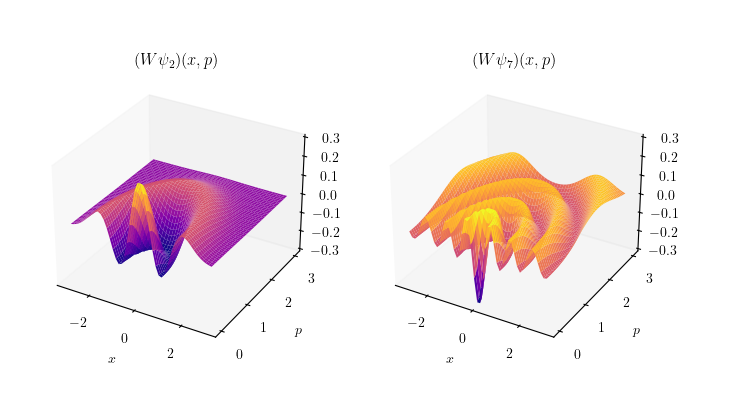
\includegraphics[width=0.9\textwidth]{
      imgs/harmonic_osc_wigner.png}
      \caption{
      Funciones de Wigner de los estados $\psi_3$ y $\psi_7$ 
      con $\hbar = 1$ y $\omega = 1$.}
      \label{fig:harmonic_osc_wigner}
    \end{figure}
  \end{frame}

  \begin{frame}
    \frametitle{Función de Wigner}

    Es común expresar la función de Wigner de un estado como
    el valor esperado de un operador $\hat\Delta(x,p)$
    llamado \textit{núcleo} o \textit{operador puntual (de
    fase)}, donde $(x,p) \in \mathcal M$.
    
    \vspace{5mm}

    \pause

    \begin{definition}
      Consideremos un estado cuántico representado por el
      operador de densidad $\hat \rho$. Su función de Wigner
      se define como:
      \begin{equation}
        W_{\hat\rho}(x,p)
        = \frac{1}{\pi \hbar} \Tr\left(
          \hat \rho \hat \Delta(x,p)
        \right).
      \end{equation}
    \end{definition}
  \end{frame}

  \begin{frame}{Operador puntual del espacio de fase}
    \begin{definition}
      El operador puntual $\hat \Delta(\xi,\eta) : \mathcal
      D \subset L^2(\R) \to L^2(\R)$, se define
      operacionalmente para $\psi \in \mathcal D$ de la
      siguiente manera:
      \begin{equation}
        \hat \Delta(\xi,\eta) \psi(x)
        = e^{\frac{2i}{\hbar} \eta(x - \xi)} \psi(2\xi - x).
      \end{equation}
    \end{definition}

    \vspace{5mm}

    \pause

    \begin{block}{Nota}
      Los operadores puntuales pueden ser expresados en
      términos de los operadores de Heisenberg-Weyl $\hat
      D(x,p) = e^{x \hat P + p \hat X}$.
    \end{block}
    
  \end{frame}

  %\begin{frame}
  %  \frametitle{Operador puntual del espacio de fase}

  %  Los operadores puntuales a su vez se pueden expresar
  %  (definir) en términos de los operadores de
  %  desplazamiento.

  %  \vspace{10pt}

  %  \begin{definition}[Operadores de desplazamiento]
  %    Los operadores de desplazamiento (operadores de
  %    Heisenberg-Weyl) 
  %    \begin{equation}
  %      \hat D(\xi,\eta) : \mathcal D \subset L^2(\R) \to
  %      L^2(\R)
  %    \end{equation}
  %    se definen como
  %    \begin{equation}
  %      \hat D(\xi,\eta) \psi(x)
  %      = e^{\frac{i}{\hbar} (\eta x - \frac{1}{2} \eta \xi)}
  %      \psi(x - \xi).
  %    \end{equation}
  %  \end{definition}
  %\end{frame}

  %\begin{frame}
  %  \frametitle{Operador puntual del espacio de fase}

  %  \begin{proposition}
  %    El operador puntual se puede expresar como la
  %    transformación unitaria del operador de paridad:
  %    \begin{equation}
  %      \hat \Delta(0,0)\psi(x) 
  %      = \psi(-x),
  %    \end{equation}
  %    por medio de los operadores de desplazamiento:
  %    \begin{equation}
  %      \hat \Delta(\xi,\eta)
  %      = \hat D(\xi,\eta) \hat\Delta(0,0) \hat
  %      D(\xi,\eta)^{*}.
  %    \end{equation}
  %  \end{proposition}
  %\end{frame}

  %\begin{frame}
  %  \frametitle{Función de Wigner}

  %  \begin{proposition}
  %    La función de Wigner de un estado $\psi$ se puede
  %    expresar como el valor esperado del operador puntual:
  %    \begin{equation}
  %      W_\psi(x,p)
  %      = \frac{1}{\pi \hbar} \braket{\psi|\hat
  %        \Delta(x,p)|\psi}.
  %    \end{equation}
  %  \end{proposition}

  %  De manera análoga, para un estado arbitrario,
  %  representado por un operador de densidad $\rho$, la
  %  función de Wigner se define como:
  %  \begin{equation}
  %    W_\psi(x,p)
  %    = \frac{1}{\pi \hbar} \Tr\left( \hat \rho \hat
  %    \Delta(x,p) \right).
  %  \end{equation}
  %\end{frame}

  \begin{frame}
    \frametitle{Propiedades de la función de Wigner}

    La función de Wigner $W_{\hat\rho}$ de un estado
    cuántico $\hat\rho$ satisface las siguientes
    propiedades:

    \vspace{5pt}

    \begin{enumerate}
      \item $W_{\hat\rho}$ es real.
      \item La integral de $W_{\hat\rho}$ sobre todo el
        espacio de fase es igual a $1$.
      \item $W_{\hat\rho}$ es \textit{covariante bajo
        traslaciones}: si $\hat\rho'$ es un estado obtenido
        por desplazar a $\hat\rho$ por $\hat D(x',p')$,
        entonces
        \begin{equation}
          W_{\hat\rho'}(x,p)
          = W_{\hat\rho}(x-x',p-p').
        \end{equation}
      \item Las integrales sobre el espacio de fase brindan
        las densidades \textit{marginales} correctas.
    \end{enumerate}

    \vspace{3mm}

    \pause

    \textbf{Observación:} Todas éstas propiedades se pueden
    plasmar en términos de los operadores puntuales.
  \end{frame}

  \begin{frame}
    \frametitle{Propiedad tomográfica de la función de
    Wigner}

    Integrando sobre el espacio de fase obtenemos densidades
    probabilísticas i.e., integrando a $W_\rho$ sobre una
    franja delimitada por las rectas paralelas
    \begin{equation*}
      ax+bp=c_1,
      \quad \text{y} \quad ax+bp=c_2,
    \end{equation*}
    obtenemos la probabilidad de observar un valor entre
    $c_1$ y $c_2$ del operador $a \hat X + b \hat P$.

    \vspace{15pt}

    \pause

    \begin{block}{Propiedad tomográfica}
      Dado un conjunto completo de marginales, podemos
      recuperar a la función de Wigner, y como consecuencia
      al estado cuántico.
    \end{block}
    

    %\vspace{15pt}

    %\pause

    %La mayoría de las propiedades mencionadas se pueden
    %obtener mediante propiedades análogas de los operadores
    %puntuales.
  \end{frame}

  

  
  \section{El espacio de fase discreto}

  \begin{frame}
    \frametitle{Generalización a sistemas finitos}

    Los sistemas que consideraremos pueden describir un
    conjunto finito de $n$ partículas de dimensión $p$, o a
    un sistema de una partícula de dimensión $d = p^{n}$:

    \begin{equation}
      \mathcal H
      = \C^{d}
      \cong \left( \C^{p} \right)^{\otimes n},
      \quad \text{donde } d = p^{n}.
    \end{equation}

    \vspace{15pt}

    \pause

    Gibbons y Wootters (2004) proponen un método basado en
    \textbf{campos finitos}. Su metodología consiste en la
    preservación de las propiedades de la función de Wigner
    en el caso continuo, en específico, la preservación de
    la propiedad tomográfica.
  \end{frame}

  \begin{frame}
    \frametitle{El espacio de fase discreto}

    \begin{definition}[Espacio de fase discreto]
      El espacio de fase discreto (DPS) $\mathcal M$,
      consiste de un espacio vectorial de dos dimensiones
      sobre un campo finito $\F$ de cardinalidad $d$. Lo
      visualizamos como una malla de $d \times d$ puntos de
      manera análoga al espacio de fase continuo.
    \end{definition}

    \vspace{10pt}

    \pause

    El uso de un campo finito le brinda al DPS una geometría
    similar a la euclideana.

    %En particular las rectas
    %paralelas no se intersectan, por dos puntos pasa
    %solamente una recta, y por cada punto pasan exactamente
    %$d+1$ rectas.

    \vspace{10pt} 

    \pause

    Identificamos al campo finito con la extensión de Galois
    $\GF(p^{n})$, así que nos limitamos a sistemas de
    dimensión $p^{n}$ donde $p$ es un número primo.
  \end{frame}

  \begin{frame}
    \frametitle{Ejemplo}

    \begin{figure}[h]
      \centering
      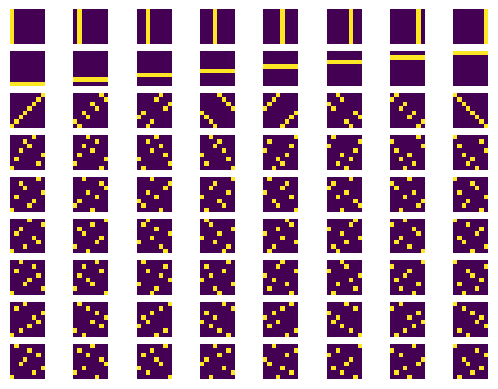
\includegraphics[width=0.5\textwidth]{imgs/GF23.png}
      \caption{Las nueve \textit{estrías de rectas} del
      espacio de discreto etiquetado por los elementos de
      $\F = \GF(2^{3})$. Ésto corresponde a un sistema de
      tres qubits.}
      \label{fig:GF23}
    \end{figure}
  \end{frame}

  \begin{frame}
    \frametitle{Operadores de desplazamiento}

    \begin{definition}[Operadores de Pauli generalizados]
      Sea $\{\ket{e_w} : w \in \F\}$ una base ortonormal de
      $\H$. Sea $\omega \in \C$ la $p$-ésima raíz primitiva
      de la unidad y sean $u, v \in \F$. Los operadores de
      Pauli generalizados se definen como:
      \begin{align}
        X(u) &: \ket{e_w} \mapsto \ket{e_{w+u}} \\
        Z(v) &: \ket{e_w} \mapsto \omega^{\tr(vw)}
        \ket{e_w}.
      \end{align}
    \end{definition}

    \pause

    \begin{definition}[Operador de desplazamiento]
      Un operador de desplazamiento arbitrario se define como
      \begin{equation}
        D(u,v) 
        = X(u) Z(v)
        \quad \text{para todo } (u,v) \in \mathcal M.
      \end{equation}
    \end{definition}
  \end{frame}

  \begin{frame}
    \frametitle{Operadores de desplazamiento}

    \begin{proposition}
      Dos operadores de desplazamiento $D(u,v)$ y $D(u',v')$
      conmutan si y solo si la forma bilineal alternante en
      $\mathcal M$ dada por
      \begin{equation}
        \langle (u,v), (u',v') \rangle
        = uv' - vu',
      \end{equation}
      se anula.
    \end{proposition}

    \pause

    \begin{proof}
      El conmutador se puede expresar como:
      \begin{equation}
        \left[
          D(u,v), D(u',v')
        \right]
        = \omega^{\tr(vu')} \left( 1 - \omega^{\langle (u,v),
        (u',v') \rangle} \right) D(u+u', v+v').
      \end{equation}
    \end{proof}
  \end{frame}

  \begin{frame}
    \frametitle{Conjuntos conmutativos de operadores de
    desplazamiento}

    El conjunto de $d-1$ operadores de desplazamiento
    etiquetados por los puntos de un rayo (ignorando el
    origen) conmutan entre si.
    
    \vspace{10pt}
    \pause
    
    Podemos diagonalizar de manera simultánea a los
    operadores de un conjunto conmutativo, obteniendo una
    base ortonormal única correspondiente a cada rayo.

    \vspace{10pt}
    \pause
    
    Existen $d + 1$ rayos en el DPS, por lo tanto obtenemos
    $d + 1$ bases ortonormales distintas.
  \end{frame}

  \begin{frame}
    \frametitle{Bases mutuamente insesgadas}

    \begin{theorem}[Bandyophyay et al]
      Si existe una partición de $d^2-1$ matrices unitarias
      mutuamente ortogonales en $d+1$ conjuntos de $d-1$ 
      matrices conmutativas, entonces existen un conjunto de
      $d+1$ bases mutuamente insesgadas (MUBs).
    \end{theorem} 

    \pause

    \begin{definition}[Bases mutuamente insesagadas]
      Las MUBs son un conjunto de bases ortonormales,
      $\mathcal B = \{\mathcal B_0, \mathcal
      B_1,\ldots,\mathcal B_k\}$ tales que 
      \begin{equation}
        \left|\braket{\psi_i|\phi_j}\right|^2
        = \frac{1}{d},
      \end{equation}
      para todo $i$ y $j$ con $\psi_i$ y $\phi_j$ de distintas
      bases.
    \end{definition}
  \end{frame}

  \begin{frame}
    \frametitle{MUBs y tomografía cuántica}

    En 1987 Ivanovic probó que un conjunto de $d+1$ MUBs es
    suficiente para determinar un estado cuántico.

    \vspace{15pt}

    \pause

    Wootters y Fields probaron en 1989 que la reconstrucción
    de un estado cuántico por medio medidas proyectivas es
    óptima cuando las bases utilizadas son MUBs, en el
    sentido de que reducen el error estadístico.

    \vspace{15pt}

    \pause

    También se les conoce como bases complementarias porque
    la información que se obtiene al medir en una base no
    nos aporta información sobre las mediciones en otra
    base.
  \end{frame}

  \section{Funciones de Wigner discretas}

  \subsection{Asignación de una estructura cuántica al DPS}

  \begin{frame}
    \frametitle{Asignación de una estructura cuántica}

    La idea principal de Gibbons y Wootters fue asignar
    estados cuánticos a \textit{cada} recta del DPS de tal
    manera que se preserva la correspondencia entre
    operadores de desplazamiento y traslaciones en el DPS.

    \vspace{5pt}

    \pause

    \begin{definition}[Malla cuántica]
      Sea $\lambda$ una recta del DPS, entonces el mapeo
      \begin{equation}
        Q : \lambda \mapsto \hat\rho \in \mathcal L(\H),
      \end{equation}
      es una \textit{malla cuántica} si para toda traslación
      $\mathcal T(a,b)$ se satisface
      \begin{equation}
        Q\left( \mathcal T(a,b) \lambda \right) 
        =
        D(a,b) Q(\lambda) D(a,b)^{*}.
      \end{equation}
    \end{definition}
  \end{frame}
  
  \subsection{Definición de la función de Wigner}

  \begin{frame}
    \frametitle{Definición de la función de Wigner}

    La función de Wigner de un estado $\hat\rho$ debe
    satisfacer la propiedad tomográfica, para el caso
    discreto ésto se expresa como:
    \begin{equation}
      \sum_{(\alpha,\beta) \in \lambda}^{}
      W_{\hat\rho}(\alpha,\beta)
      = \Tr\left( \hat\rho Q(\lambda) \right),
    \end{equation}
    para toda recta $\lambda$ del espacio de fase discreto.
    Ésta propiedad junto con la propiedad de
    \textit{normalización} determinan a la función de
    Wigner.

    \vspace{15pt}

    \pause

    Usando las propiedades del DPS podemos invertir ésta
    relación para obtener una expresión para
    $W_{\hat\rho}(\alpha,\beta)$.
  \end{frame}

  \begin{frame}
    \frametitle{Definición de la función de Wigner}

    \begin{definition}[Función de Wigner discreta]
      Sea $\hat\rho$ un estado cuántico. Dada una malla
      cuántica $Q$, definimos su función de Wigner
      discreta como:
      \begin{equation}
        W_{\hat\rho}(\alpha,\beta)
        = \frac{1}{d} \Tr\left(
          \hat\rho \hat A(\alpha,\beta)
        \right),
      \end{equation}
      donde $(\alpha,\beta) \in \mathcal M$ y 
      \begin{equation}
        \hat A(\alpha,\beta)
        = \sum_{\lambda \ni (\alpha,\beta)}^{}
        Q(\lambda) - I.
      \end{equation}
    \end{definition}
  \end{frame}

  \begin{frame}
    \frametitle{Propiedades de la función de Wigner
    discreta}

    \begin{enumerate}
      \item La función de Wigner es real.
      \item La suma de $W_{\hat\rho}$ sobre cualquier recta
        $\lambda$ es igual al valor esperado de $Q(\lambda)$
        en el estado $\hat\rho$.
      \item La suma de $W_{\hat\rho}$ sobre todo el espacio
        de fase es igual a $1$.
      \item La función de Wigner es covariante bajo
        traslaciones.
    \end{enumerate}

    \vspace{10pt}

    Dada la función de Wigner, podemos recuperar al estado
    cuántico utilizando los operadores puntuales.
    \begin{equation}
      \hat\rho
      = \sum_{(\alpha,\beta) \in \mathcal M}^{}
      W_{\hat\rho}(\alpha,\beta) \hat A(\alpha,\beta).
    \end{equation}
  \end{frame}

  \begin{frame}
    \frametitle{Ejemplo}

    Consideremos un sistema de dos qubits cuyo espacio de
    Hilbert es $\H = \C^2 \otimes \C^2 \cong \C^{4}$. El
    campo finito es $\F = \GF(2^2) =
    \{0,1,\alpha,\alpha+1\}$.
    \begin{figure}[h]
      \centering
      \scalebox{0.4}{
        %% Creator: Matplotlib, PGF backend
%%
%% To include the figure in your LaTeX document, write
%%   \input{<filename>.pgf}
%%
%% Make sure the required packages are loaded in your preamble
%%   \usepackage{pgf}
%%
%% Also ensure that all the required font packages are loaded; for instance,
%% the lmodern package is sometimes necessary when using math font.
%%   \usepackage{lmodern}
%%
%% Figures using additional raster images can only be included by \input if
%% they are in the same directory as the main LaTeX file. For loading figures
%% from other directories you can use the `import` package
%%   \usepackage{import}
%%
%% and then include the figures with
%%   \import{<path to file>}{<filename>.pgf}
%%
%% Matplotlib used the following preamble
%%   
%%   \makeatletter\@ifpackageloaded{underscore}{}{\usepackage[strings]{underscore}}\makeatother
%%
\begingroup%
\makeatletter%
\begin{pgfpicture}%
\pgfpathrectangle{\pgfpointorigin}{\pgfqpoint{4.500000in}{4.500000in}}%
\pgfusepath{use as bounding box, clip}%
\begin{pgfscope}%
\pgfsetbuttcap%
\pgfsetmiterjoin%
\definecolor{currentfill}{rgb}{1.000000,1.000000,1.000000}%
\pgfsetfillcolor{currentfill}%
\pgfsetlinewidth{0.000000pt}%
\definecolor{currentstroke}{rgb}{1.000000,1.000000,1.000000}%
\pgfsetstrokecolor{currentstroke}%
\pgfsetdash{}{0pt}%
\pgfpathmoveto{\pgfqpoint{0.000000in}{0.000000in}}%
\pgfpathlineto{\pgfqpoint{4.500000in}{0.000000in}}%
\pgfpathlineto{\pgfqpoint{4.500000in}{4.500000in}}%
\pgfpathlineto{\pgfqpoint{0.000000in}{4.500000in}}%
\pgfpathlineto{\pgfqpoint{0.000000in}{0.000000in}}%
\pgfpathclose%
\pgfusepath{fill}%
\end{pgfscope}%
\begin{pgfscope}%
\pgfsetbuttcap%
\pgfsetmiterjoin%
\definecolor{currentfill}{rgb}{1.000000,1.000000,1.000000}%
\pgfsetfillcolor{currentfill}%
\pgfsetlinewidth{0.000000pt}%
\definecolor{currentstroke}{rgb}{0.000000,0.000000,0.000000}%
\pgfsetstrokecolor{currentstroke}%
\pgfsetstrokeopacity{0.000000}%
\pgfsetdash{}{0pt}%
\pgfpathmoveto{\pgfqpoint{0.562500in}{0.495000in}}%
\pgfpathlineto{\pgfqpoint{4.050000in}{0.495000in}}%
\pgfpathlineto{\pgfqpoint{4.050000in}{3.960000in}}%
\pgfpathlineto{\pgfqpoint{0.562500in}{3.960000in}}%
\pgfpathlineto{\pgfqpoint{0.562500in}{0.495000in}}%
\pgfpathclose%
\pgfusepath{fill}%
\end{pgfscope}%
\begin{pgfscope}%
\pgfsetbuttcap%
\pgfsetroundjoin%
\definecolor{currentfill}{rgb}{0.000000,0.000000,0.000000}%
\pgfsetfillcolor{currentfill}%
\pgfsetlinewidth{0.803000pt}%
\definecolor{currentstroke}{rgb}{0.000000,0.000000,0.000000}%
\pgfsetstrokecolor{currentstroke}%
\pgfsetdash{}{0pt}%
\pgfsys@defobject{currentmarker}{\pgfqpoint{0.000000in}{-0.048611in}}{\pgfqpoint{0.000000in}{0.000000in}}{%
\pgfpathmoveto{\pgfqpoint{0.000000in}{0.000000in}}%
\pgfpathlineto{\pgfqpoint{0.000000in}{-0.048611in}}%
\pgfusepath{stroke,fill}%
}%
\begin{pgfscope}%
\pgfsys@transformshift{0.721023in}{0.495000in}%
\pgfsys@useobject{currentmarker}{}%
\end{pgfscope}%
\end{pgfscope}%
\begin{pgfscope}%
\definecolor{textcolor}{rgb}{0.000000,0.000000,0.000000}%
\pgfsetstrokecolor{textcolor}%
\pgfsetfillcolor{textcolor}%
\pgftext[x=0.721023in,y=0.397778in,,top]{\color{textcolor}\rmfamily\fontsize{10.000000}{12.000000}\selectfont \(\displaystyle 0\)}%
\end{pgfscope}%
\begin{pgfscope}%
\pgfsetbuttcap%
\pgfsetroundjoin%
\definecolor{currentfill}{rgb}{0.000000,0.000000,0.000000}%
\pgfsetfillcolor{currentfill}%
\pgfsetlinewidth{0.803000pt}%
\definecolor{currentstroke}{rgb}{0.000000,0.000000,0.000000}%
\pgfsetstrokecolor{currentstroke}%
\pgfsetdash{}{0pt}%
\pgfsys@defobject{currentmarker}{\pgfqpoint{0.000000in}{-0.048611in}}{\pgfqpoint{0.000000in}{0.000000in}}{%
\pgfpathmoveto{\pgfqpoint{0.000000in}{0.000000in}}%
\pgfpathlineto{\pgfqpoint{0.000000in}{-0.048611in}}%
\pgfusepath{stroke,fill}%
}%
\begin{pgfscope}%
\pgfsys@transformshift{1.777841in}{0.495000in}%
\pgfsys@useobject{currentmarker}{}%
\end{pgfscope}%
\end{pgfscope}%
\begin{pgfscope}%
\definecolor{textcolor}{rgb}{0.000000,0.000000,0.000000}%
\pgfsetstrokecolor{textcolor}%
\pgfsetfillcolor{textcolor}%
\pgftext[x=1.777841in,y=0.397778in,,top]{\color{textcolor}\rmfamily\fontsize{10.000000}{12.000000}\selectfont \(\displaystyle a\)}%
\end{pgfscope}%
\begin{pgfscope}%
\pgfsetbuttcap%
\pgfsetroundjoin%
\definecolor{currentfill}{rgb}{0.000000,0.000000,0.000000}%
\pgfsetfillcolor{currentfill}%
\pgfsetlinewidth{0.803000pt}%
\definecolor{currentstroke}{rgb}{0.000000,0.000000,0.000000}%
\pgfsetstrokecolor{currentstroke}%
\pgfsetdash{}{0pt}%
\pgfsys@defobject{currentmarker}{\pgfqpoint{0.000000in}{-0.048611in}}{\pgfqpoint{0.000000in}{0.000000in}}{%
\pgfpathmoveto{\pgfqpoint{0.000000in}{0.000000in}}%
\pgfpathlineto{\pgfqpoint{0.000000in}{-0.048611in}}%
\pgfusepath{stroke,fill}%
}%
\begin{pgfscope}%
\pgfsys@transformshift{2.834659in}{0.495000in}%
\pgfsys@useobject{currentmarker}{}%
\end{pgfscope}%
\end{pgfscope}%
\begin{pgfscope}%
\definecolor{textcolor}{rgb}{0.000000,0.000000,0.000000}%
\pgfsetstrokecolor{textcolor}%
\pgfsetfillcolor{textcolor}%
\pgftext[x=2.834659in,y=0.397778in,,top]{\color{textcolor}\rmfamily\fontsize{10.000000}{12.000000}\selectfont \(\displaystyle a + 1\)}%
\end{pgfscope}%
\begin{pgfscope}%
\pgfsetbuttcap%
\pgfsetroundjoin%
\definecolor{currentfill}{rgb}{0.000000,0.000000,0.000000}%
\pgfsetfillcolor{currentfill}%
\pgfsetlinewidth{0.803000pt}%
\definecolor{currentstroke}{rgb}{0.000000,0.000000,0.000000}%
\pgfsetstrokecolor{currentstroke}%
\pgfsetdash{}{0pt}%
\pgfsys@defobject{currentmarker}{\pgfqpoint{0.000000in}{-0.048611in}}{\pgfqpoint{0.000000in}{0.000000in}}{%
\pgfpathmoveto{\pgfqpoint{0.000000in}{0.000000in}}%
\pgfpathlineto{\pgfqpoint{0.000000in}{-0.048611in}}%
\pgfusepath{stroke,fill}%
}%
\begin{pgfscope}%
\pgfsys@transformshift{3.891477in}{0.495000in}%
\pgfsys@useobject{currentmarker}{}%
\end{pgfscope}%
\end{pgfscope}%
\begin{pgfscope}%
\definecolor{textcolor}{rgb}{0.000000,0.000000,0.000000}%
\pgfsetstrokecolor{textcolor}%
\pgfsetfillcolor{textcolor}%
\pgftext[x=3.891477in,y=0.397778in,,top]{\color{textcolor}\rmfamily\fontsize{10.000000}{12.000000}\selectfont \(\displaystyle 1\)}%
\end{pgfscope}%
\begin{pgfscope}%
\pgfsetbuttcap%
\pgfsetroundjoin%
\definecolor{currentfill}{rgb}{0.000000,0.000000,0.000000}%
\pgfsetfillcolor{currentfill}%
\pgfsetlinewidth{0.803000pt}%
\definecolor{currentstroke}{rgb}{0.000000,0.000000,0.000000}%
\pgfsetstrokecolor{currentstroke}%
\pgfsetdash{}{0pt}%
\pgfsys@defobject{currentmarker}{\pgfqpoint{-0.048611in}{0.000000in}}{\pgfqpoint{-0.000000in}{0.000000in}}{%
\pgfpathmoveto{\pgfqpoint{-0.000000in}{0.000000in}}%
\pgfpathlineto{\pgfqpoint{-0.048611in}{0.000000in}}%
\pgfusepath{stroke,fill}%
}%
\begin{pgfscope}%
\pgfsys@transformshift{0.562500in}{0.652500in}%
\pgfsys@useobject{currentmarker}{}%
\end{pgfscope}%
\end{pgfscope}%
\begin{pgfscope}%
\definecolor{textcolor}{rgb}{0.000000,0.000000,0.000000}%
\pgfsetstrokecolor{textcolor}%
\pgfsetfillcolor{textcolor}%
\pgftext[x=0.395833in, y=0.604275in, left, base]{\color{textcolor}\rmfamily\fontsize{10.000000}{12.000000}\selectfont \(\displaystyle 0\)}%
\end{pgfscope}%
\begin{pgfscope}%
\pgfsetbuttcap%
\pgfsetroundjoin%
\definecolor{currentfill}{rgb}{0.000000,0.000000,0.000000}%
\pgfsetfillcolor{currentfill}%
\pgfsetlinewidth{0.803000pt}%
\definecolor{currentstroke}{rgb}{0.000000,0.000000,0.000000}%
\pgfsetstrokecolor{currentstroke}%
\pgfsetdash{}{0pt}%
\pgfsys@defobject{currentmarker}{\pgfqpoint{-0.048611in}{0.000000in}}{\pgfqpoint{-0.000000in}{0.000000in}}{%
\pgfpathmoveto{\pgfqpoint{-0.000000in}{0.000000in}}%
\pgfpathlineto{\pgfqpoint{-0.048611in}{0.000000in}}%
\pgfusepath{stroke,fill}%
}%
\begin{pgfscope}%
\pgfsys@transformshift{0.562500in}{1.702500in}%
\pgfsys@useobject{currentmarker}{}%
\end{pgfscope}%
\end{pgfscope}%
\begin{pgfscope}%
\definecolor{textcolor}{rgb}{0.000000,0.000000,0.000000}%
\pgfsetstrokecolor{textcolor}%
\pgfsetfillcolor{textcolor}%
\pgftext[x=0.391863in, y=1.654275in, left, base]{\color{textcolor}\rmfamily\fontsize{10.000000}{12.000000}\selectfont \(\displaystyle a\)}%
\end{pgfscope}%
\begin{pgfscope}%
\pgfsetbuttcap%
\pgfsetroundjoin%
\definecolor{currentfill}{rgb}{0.000000,0.000000,0.000000}%
\pgfsetfillcolor{currentfill}%
\pgfsetlinewidth{0.803000pt}%
\definecolor{currentstroke}{rgb}{0.000000,0.000000,0.000000}%
\pgfsetstrokecolor{currentstroke}%
\pgfsetdash{}{0pt}%
\pgfsys@defobject{currentmarker}{\pgfqpoint{-0.048611in}{0.000000in}}{\pgfqpoint{-0.000000in}{0.000000in}}{%
\pgfpathmoveto{\pgfqpoint{-0.000000in}{0.000000in}}%
\pgfpathlineto{\pgfqpoint{-0.048611in}{0.000000in}}%
\pgfusepath{stroke,fill}%
}%
\begin{pgfscope}%
\pgfsys@transformshift{0.562500in}{2.752500in}%
\pgfsys@useobject{currentmarker}{}%
\end{pgfscope}%
\end{pgfscope}%
\begin{pgfscope}%
\definecolor{textcolor}{rgb}{0.000000,0.000000,0.000000}%
\pgfsetstrokecolor{textcolor}%
\pgfsetfillcolor{textcolor}%
\pgftext[x=0.152666in, y=2.704275in, left, base]{\color{textcolor}\rmfamily\fontsize{10.000000}{12.000000}\selectfont \(\displaystyle a + 1\)}%
\end{pgfscope}%
\begin{pgfscope}%
\pgfsetbuttcap%
\pgfsetroundjoin%
\definecolor{currentfill}{rgb}{0.000000,0.000000,0.000000}%
\pgfsetfillcolor{currentfill}%
\pgfsetlinewidth{0.803000pt}%
\definecolor{currentstroke}{rgb}{0.000000,0.000000,0.000000}%
\pgfsetstrokecolor{currentstroke}%
\pgfsetdash{}{0pt}%
\pgfsys@defobject{currentmarker}{\pgfqpoint{-0.048611in}{0.000000in}}{\pgfqpoint{-0.000000in}{0.000000in}}{%
\pgfpathmoveto{\pgfqpoint{-0.000000in}{0.000000in}}%
\pgfpathlineto{\pgfqpoint{-0.048611in}{0.000000in}}%
\pgfusepath{stroke,fill}%
}%
\begin{pgfscope}%
\pgfsys@transformshift{0.562500in}{3.802500in}%
\pgfsys@useobject{currentmarker}{}%
\end{pgfscope}%
\end{pgfscope}%
\begin{pgfscope}%
\definecolor{textcolor}{rgb}{0.000000,0.000000,0.000000}%
\pgfsetstrokecolor{textcolor}%
\pgfsetfillcolor{textcolor}%
\pgftext[x=0.395833in, y=3.754275in, left, base]{\color{textcolor}\rmfamily\fontsize{10.000000}{12.000000}\selectfont \(\displaystyle 1\)}%
\end{pgfscope}%
\begin{pgfscope}%
\pgfpathrectangle{\pgfqpoint{0.562500in}{0.495000in}}{\pgfqpoint{3.487500in}{3.465000in}}%
\pgfusepath{clip}%
\pgfsetrectcap%
\pgfsetroundjoin%
\pgfsetlinewidth{0.200750pt}%
\definecolor{currentstroke}{rgb}{0.121569,0.466667,0.705882}%
\pgfsetstrokecolor{currentstroke}%
\pgfsetstrokeopacity{0.800000}%
\pgfsetdash{}{0pt}%
\pgfpathmoveto{\pgfqpoint{0.721023in}{0.652500in}}%
\pgfpathlineto{\pgfqpoint{0.721023in}{1.702500in}}%
\pgfpathlineto{\pgfqpoint{0.721023in}{2.752500in}}%
\pgfpathlineto{\pgfqpoint{0.721023in}{3.802500in}}%
\pgfusepath{stroke}%
\end{pgfscope}%
\begin{pgfscope}%
\pgfpathrectangle{\pgfqpoint{0.562500in}{0.495000in}}{\pgfqpoint{3.487500in}{3.465000in}}%
\pgfusepath{clip}%
\pgfsetbuttcap%
\pgfsetroundjoin%
\definecolor{currentfill}{rgb}{0.121569,0.466667,0.705882}%
\pgfsetfillcolor{currentfill}%
\pgfsetfillopacity{0.800000}%
\pgfsetlinewidth{1.003750pt}%
\definecolor{currentstroke}{rgb}{0.121569,0.466667,0.705882}%
\pgfsetstrokecolor{currentstroke}%
\pgfsetstrokeopacity{0.800000}%
\pgfsetdash{}{0pt}%
\pgfsys@defobject{currentmarker}{\pgfqpoint{-0.041667in}{-0.041667in}}{\pgfqpoint{0.041667in}{0.041667in}}{%
\pgfpathmoveto{\pgfqpoint{0.000000in}{-0.041667in}}%
\pgfpathcurveto{\pgfqpoint{0.011050in}{-0.041667in}}{\pgfqpoint{0.021649in}{-0.037276in}}{\pgfqpoint{0.029463in}{-0.029463in}}%
\pgfpathcurveto{\pgfqpoint{0.037276in}{-0.021649in}}{\pgfqpoint{0.041667in}{-0.011050in}}{\pgfqpoint{0.041667in}{0.000000in}}%
\pgfpathcurveto{\pgfqpoint{0.041667in}{0.011050in}}{\pgfqpoint{0.037276in}{0.021649in}}{\pgfqpoint{0.029463in}{0.029463in}}%
\pgfpathcurveto{\pgfqpoint{0.021649in}{0.037276in}}{\pgfqpoint{0.011050in}{0.041667in}}{\pgfqpoint{0.000000in}{0.041667in}}%
\pgfpathcurveto{\pgfqpoint{-0.011050in}{0.041667in}}{\pgfqpoint{-0.021649in}{0.037276in}}{\pgfqpoint{-0.029463in}{0.029463in}}%
\pgfpathcurveto{\pgfqpoint{-0.037276in}{0.021649in}}{\pgfqpoint{-0.041667in}{0.011050in}}{\pgfqpoint{-0.041667in}{0.000000in}}%
\pgfpathcurveto{\pgfqpoint{-0.041667in}{-0.011050in}}{\pgfqpoint{-0.037276in}{-0.021649in}}{\pgfqpoint{-0.029463in}{-0.029463in}}%
\pgfpathcurveto{\pgfqpoint{-0.021649in}{-0.037276in}}{\pgfqpoint{-0.011050in}{-0.041667in}}{\pgfqpoint{0.000000in}{-0.041667in}}%
\pgfpathlineto{\pgfqpoint{0.000000in}{-0.041667in}}%
\pgfpathclose%
\pgfusepath{stroke,fill}%
}%
\begin{pgfscope}%
\pgfsys@transformshift{0.721023in}{0.652500in}%
\pgfsys@useobject{currentmarker}{}%
\end{pgfscope}%
\begin{pgfscope}%
\pgfsys@transformshift{0.721023in}{1.702500in}%
\pgfsys@useobject{currentmarker}{}%
\end{pgfscope}%
\begin{pgfscope}%
\pgfsys@transformshift{0.721023in}{2.752500in}%
\pgfsys@useobject{currentmarker}{}%
\end{pgfscope}%
\begin{pgfscope}%
\pgfsys@transformshift{0.721023in}{3.802500in}%
\pgfsys@useobject{currentmarker}{}%
\end{pgfscope}%
\end{pgfscope}%
\begin{pgfscope}%
\pgfpathrectangle{\pgfqpoint{0.562500in}{0.495000in}}{\pgfqpoint{3.487500in}{3.465000in}}%
\pgfusepath{clip}%
\pgfsetrectcap%
\pgfsetroundjoin%
\pgfsetlinewidth{0.200750pt}%
\definecolor{currentstroke}{rgb}{1.000000,0.498039,0.054902}%
\pgfsetstrokecolor{currentstroke}%
\pgfsetstrokeopacity{0.800000}%
\pgfsetdash{}{0pt}%
\pgfpathmoveto{\pgfqpoint{0.721023in}{0.652500in}}%
\pgfpathlineto{\pgfqpoint{1.777841in}{0.652500in}}%
\pgfpathlineto{\pgfqpoint{2.834659in}{0.652500in}}%
\pgfpathlineto{\pgfqpoint{3.891477in}{0.652500in}}%
\pgfusepath{stroke}%
\end{pgfscope}%
\begin{pgfscope}%
\pgfpathrectangle{\pgfqpoint{0.562500in}{0.495000in}}{\pgfqpoint{3.487500in}{3.465000in}}%
\pgfusepath{clip}%
\pgfsetbuttcap%
\pgfsetroundjoin%
\definecolor{currentfill}{rgb}{1.000000,0.498039,0.054902}%
\pgfsetfillcolor{currentfill}%
\pgfsetfillopacity{0.800000}%
\pgfsetlinewidth{1.003750pt}%
\definecolor{currentstroke}{rgb}{1.000000,0.498039,0.054902}%
\pgfsetstrokecolor{currentstroke}%
\pgfsetstrokeopacity{0.800000}%
\pgfsetdash{}{0pt}%
\pgfsys@defobject{currentmarker}{\pgfqpoint{-0.041667in}{-0.041667in}}{\pgfqpoint{0.041667in}{0.041667in}}{%
\pgfpathmoveto{\pgfqpoint{0.000000in}{-0.041667in}}%
\pgfpathcurveto{\pgfqpoint{0.011050in}{-0.041667in}}{\pgfqpoint{0.021649in}{-0.037276in}}{\pgfqpoint{0.029463in}{-0.029463in}}%
\pgfpathcurveto{\pgfqpoint{0.037276in}{-0.021649in}}{\pgfqpoint{0.041667in}{-0.011050in}}{\pgfqpoint{0.041667in}{0.000000in}}%
\pgfpathcurveto{\pgfqpoint{0.041667in}{0.011050in}}{\pgfqpoint{0.037276in}{0.021649in}}{\pgfqpoint{0.029463in}{0.029463in}}%
\pgfpathcurveto{\pgfqpoint{0.021649in}{0.037276in}}{\pgfqpoint{0.011050in}{0.041667in}}{\pgfqpoint{0.000000in}{0.041667in}}%
\pgfpathcurveto{\pgfqpoint{-0.011050in}{0.041667in}}{\pgfqpoint{-0.021649in}{0.037276in}}{\pgfqpoint{-0.029463in}{0.029463in}}%
\pgfpathcurveto{\pgfqpoint{-0.037276in}{0.021649in}}{\pgfqpoint{-0.041667in}{0.011050in}}{\pgfqpoint{-0.041667in}{0.000000in}}%
\pgfpathcurveto{\pgfqpoint{-0.041667in}{-0.011050in}}{\pgfqpoint{-0.037276in}{-0.021649in}}{\pgfqpoint{-0.029463in}{-0.029463in}}%
\pgfpathcurveto{\pgfqpoint{-0.021649in}{-0.037276in}}{\pgfqpoint{-0.011050in}{-0.041667in}}{\pgfqpoint{0.000000in}{-0.041667in}}%
\pgfpathlineto{\pgfqpoint{0.000000in}{-0.041667in}}%
\pgfpathclose%
\pgfusepath{stroke,fill}%
}%
\begin{pgfscope}%
\pgfsys@transformshift{0.721023in}{0.652500in}%
\pgfsys@useobject{currentmarker}{}%
\end{pgfscope}%
\begin{pgfscope}%
\pgfsys@transformshift{1.777841in}{0.652500in}%
\pgfsys@useobject{currentmarker}{}%
\end{pgfscope}%
\begin{pgfscope}%
\pgfsys@transformshift{2.834659in}{0.652500in}%
\pgfsys@useobject{currentmarker}{}%
\end{pgfscope}%
\begin{pgfscope}%
\pgfsys@transformshift{3.891477in}{0.652500in}%
\pgfsys@useobject{currentmarker}{}%
\end{pgfscope}%
\end{pgfscope}%
\begin{pgfscope}%
\pgfpathrectangle{\pgfqpoint{0.562500in}{0.495000in}}{\pgfqpoint{3.487500in}{3.465000in}}%
\pgfusepath{clip}%
\pgfsetrectcap%
\pgfsetroundjoin%
\pgfsetlinewidth{0.200750pt}%
\definecolor{currentstroke}{rgb}{0.172549,0.627451,0.172549}%
\pgfsetstrokecolor{currentstroke}%
\pgfsetstrokeopacity{0.800000}%
\pgfsetdash{}{0pt}%
\pgfpathmoveto{\pgfqpoint{0.721023in}{0.652500in}}%
\pgfpathlineto{\pgfqpoint{1.777841in}{2.752500in}}%
\pgfpathlineto{\pgfqpoint{2.834659in}{3.802500in}}%
\pgfpathlineto{\pgfqpoint{3.891477in}{1.702500in}}%
\pgfusepath{stroke}%
\end{pgfscope}%
\begin{pgfscope}%
\pgfpathrectangle{\pgfqpoint{0.562500in}{0.495000in}}{\pgfqpoint{3.487500in}{3.465000in}}%
\pgfusepath{clip}%
\pgfsetbuttcap%
\pgfsetroundjoin%
\definecolor{currentfill}{rgb}{0.172549,0.627451,0.172549}%
\pgfsetfillcolor{currentfill}%
\pgfsetfillopacity{0.800000}%
\pgfsetlinewidth{1.003750pt}%
\definecolor{currentstroke}{rgb}{0.172549,0.627451,0.172549}%
\pgfsetstrokecolor{currentstroke}%
\pgfsetstrokeopacity{0.800000}%
\pgfsetdash{}{0pt}%
\pgfsys@defobject{currentmarker}{\pgfqpoint{-0.041667in}{-0.041667in}}{\pgfqpoint{0.041667in}{0.041667in}}{%
\pgfpathmoveto{\pgfqpoint{0.000000in}{-0.041667in}}%
\pgfpathcurveto{\pgfqpoint{0.011050in}{-0.041667in}}{\pgfqpoint{0.021649in}{-0.037276in}}{\pgfqpoint{0.029463in}{-0.029463in}}%
\pgfpathcurveto{\pgfqpoint{0.037276in}{-0.021649in}}{\pgfqpoint{0.041667in}{-0.011050in}}{\pgfqpoint{0.041667in}{0.000000in}}%
\pgfpathcurveto{\pgfqpoint{0.041667in}{0.011050in}}{\pgfqpoint{0.037276in}{0.021649in}}{\pgfqpoint{0.029463in}{0.029463in}}%
\pgfpathcurveto{\pgfqpoint{0.021649in}{0.037276in}}{\pgfqpoint{0.011050in}{0.041667in}}{\pgfqpoint{0.000000in}{0.041667in}}%
\pgfpathcurveto{\pgfqpoint{-0.011050in}{0.041667in}}{\pgfqpoint{-0.021649in}{0.037276in}}{\pgfqpoint{-0.029463in}{0.029463in}}%
\pgfpathcurveto{\pgfqpoint{-0.037276in}{0.021649in}}{\pgfqpoint{-0.041667in}{0.011050in}}{\pgfqpoint{-0.041667in}{0.000000in}}%
\pgfpathcurveto{\pgfqpoint{-0.041667in}{-0.011050in}}{\pgfqpoint{-0.037276in}{-0.021649in}}{\pgfqpoint{-0.029463in}{-0.029463in}}%
\pgfpathcurveto{\pgfqpoint{-0.021649in}{-0.037276in}}{\pgfqpoint{-0.011050in}{-0.041667in}}{\pgfqpoint{0.000000in}{-0.041667in}}%
\pgfpathlineto{\pgfqpoint{0.000000in}{-0.041667in}}%
\pgfpathclose%
\pgfusepath{stroke,fill}%
}%
\begin{pgfscope}%
\pgfsys@transformshift{0.721023in}{0.652500in}%
\pgfsys@useobject{currentmarker}{}%
\end{pgfscope}%
\begin{pgfscope}%
\pgfsys@transformshift{1.777841in}{2.752500in}%
\pgfsys@useobject{currentmarker}{}%
\end{pgfscope}%
\begin{pgfscope}%
\pgfsys@transformshift{2.834659in}{3.802500in}%
\pgfsys@useobject{currentmarker}{}%
\end{pgfscope}%
\begin{pgfscope}%
\pgfsys@transformshift{3.891477in}{1.702500in}%
\pgfsys@useobject{currentmarker}{}%
\end{pgfscope}%
\end{pgfscope}%
\begin{pgfscope}%
\pgfpathrectangle{\pgfqpoint{0.562500in}{0.495000in}}{\pgfqpoint{3.487500in}{3.465000in}}%
\pgfusepath{clip}%
\pgfsetrectcap%
\pgfsetroundjoin%
\pgfsetlinewidth{0.200750pt}%
\definecolor{currentstroke}{rgb}{0.839216,0.152941,0.156863}%
\pgfsetstrokecolor{currentstroke}%
\pgfsetstrokeopacity{0.200000}%
\pgfsetdash{}{0pt}%
\pgfpathmoveto{\pgfqpoint{0.721023in}{0.652500in}}%
\pgfpathlineto{\pgfqpoint{1.777841in}{3.802500in}}%
\pgfpathlineto{\pgfqpoint{2.834659in}{1.702500in}}%
\pgfpathlineto{\pgfqpoint{3.891477in}{2.752500in}}%
\pgfusepath{stroke}%
\end{pgfscope}%
\begin{pgfscope}%
\pgfpathrectangle{\pgfqpoint{0.562500in}{0.495000in}}{\pgfqpoint{3.487500in}{3.465000in}}%
\pgfusepath{clip}%
\pgfsetbuttcap%
\pgfsetroundjoin%
\definecolor{currentfill}{rgb}{0.839216,0.152941,0.156863}%
\pgfsetfillcolor{currentfill}%
\pgfsetfillopacity{0.200000}%
\pgfsetlinewidth{1.003750pt}%
\definecolor{currentstroke}{rgb}{0.839216,0.152941,0.156863}%
\pgfsetstrokecolor{currentstroke}%
\pgfsetstrokeopacity{0.200000}%
\pgfsetdash{}{0pt}%
\pgfsys@defobject{currentmarker}{\pgfqpoint{-0.041667in}{-0.041667in}}{\pgfqpoint{0.041667in}{0.041667in}}{%
\pgfpathmoveto{\pgfqpoint{0.000000in}{-0.041667in}}%
\pgfpathcurveto{\pgfqpoint{0.011050in}{-0.041667in}}{\pgfqpoint{0.021649in}{-0.037276in}}{\pgfqpoint{0.029463in}{-0.029463in}}%
\pgfpathcurveto{\pgfqpoint{0.037276in}{-0.021649in}}{\pgfqpoint{0.041667in}{-0.011050in}}{\pgfqpoint{0.041667in}{0.000000in}}%
\pgfpathcurveto{\pgfqpoint{0.041667in}{0.011050in}}{\pgfqpoint{0.037276in}{0.021649in}}{\pgfqpoint{0.029463in}{0.029463in}}%
\pgfpathcurveto{\pgfqpoint{0.021649in}{0.037276in}}{\pgfqpoint{0.011050in}{0.041667in}}{\pgfqpoint{0.000000in}{0.041667in}}%
\pgfpathcurveto{\pgfqpoint{-0.011050in}{0.041667in}}{\pgfqpoint{-0.021649in}{0.037276in}}{\pgfqpoint{-0.029463in}{0.029463in}}%
\pgfpathcurveto{\pgfqpoint{-0.037276in}{0.021649in}}{\pgfqpoint{-0.041667in}{0.011050in}}{\pgfqpoint{-0.041667in}{0.000000in}}%
\pgfpathcurveto{\pgfqpoint{-0.041667in}{-0.011050in}}{\pgfqpoint{-0.037276in}{-0.021649in}}{\pgfqpoint{-0.029463in}{-0.029463in}}%
\pgfpathcurveto{\pgfqpoint{-0.021649in}{-0.037276in}}{\pgfqpoint{-0.011050in}{-0.041667in}}{\pgfqpoint{0.000000in}{-0.041667in}}%
\pgfpathlineto{\pgfqpoint{0.000000in}{-0.041667in}}%
\pgfpathclose%
\pgfusepath{stroke,fill}%
}%
\begin{pgfscope}%
\pgfsys@transformshift{0.721023in}{0.652500in}%
\pgfsys@useobject{currentmarker}{}%
\end{pgfscope}%
\begin{pgfscope}%
\pgfsys@transformshift{1.777841in}{3.802500in}%
\pgfsys@useobject{currentmarker}{}%
\end{pgfscope}%
\begin{pgfscope}%
\pgfsys@transformshift{2.834659in}{1.702500in}%
\pgfsys@useobject{currentmarker}{}%
\end{pgfscope}%
\begin{pgfscope}%
\pgfsys@transformshift{3.891477in}{2.752500in}%
\pgfsys@useobject{currentmarker}{}%
\end{pgfscope}%
\end{pgfscope}%
\begin{pgfscope}%
\pgfpathrectangle{\pgfqpoint{0.562500in}{0.495000in}}{\pgfqpoint{3.487500in}{3.465000in}}%
\pgfusepath{clip}%
\pgfsetrectcap%
\pgfsetroundjoin%
\pgfsetlinewidth{0.200750pt}%
\definecolor{currentstroke}{rgb}{0.580392,0.403922,0.741176}%
\pgfsetstrokecolor{currentstroke}%
\pgfsetstrokeopacity{0.800000}%
\pgfsetdash{}{0pt}%
\pgfpathmoveto{\pgfqpoint{0.721023in}{0.652500in}}%
\pgfpathlineto{\pgfqpoint{1.777841in}{1.702500in}}%
\pgfpathlineto{\pgfqpoint{2.834659in}{2.752500in}}%
\pgfpathlineto{\pgfqpoint{3.891477in}{3.802500in}}%
\pgfusepath{stroke}%
\end{pgfscope}%
\begin{pgfscope}%
\pgfpathrectangle{\pgfqpoint{0.562500in}{0.495000in}}{\pgfqpoint{3.487500in}{3.465000in}}%
\pgfusepath{clip}%
\pgfsetbuttcap%
\pgfsetroundjoin%
\definecolor{currentfill}{rgb}{0.580392,0.403922,0.741176}%
\pgfsetfillcolor{currentfill}%
\pgfsetfillopacity{0.800000}%
\pgfsetlinewidth{1.003750pt}%
\definecolor{currentstroke}{rgb}{0.580392,0.403922,0.741176}%
\pgfsetstrokecolor{currentstroke}%
\pgfsetstrokeopacity{0.800000}%
\pgfsetdash{}{0pt}%
\pgfsys@defobject{currentmarker}{\pgfqpoint{-0.041667in}{-0.041667in}}{\pgfqpoint{0.041667in}{0.041667in}}{%
\pgfpathmoveto{\pgfqpoint{0.000000in}{-0.041667in}}%
\pgfpathcurveto{\pgfqpoint{0.011050in}{-0.041667in}}{\pgfqpoint{0.021649in}{-0.037276in}}{\pgfqpoint{0.029463in}{-0.029463in}}%
\pgfpathcurveto{\pgfqpoint{0.037276in}{-0.021649in}}{\pgfqpoint{0.041667in}{-0.011050in}}{\pgfqpoint{0.041667in}{0.000000in}}%
\pgfpathcurveto{\pgfqpoint{0.041667in}{0.011050in}}{\pgfqpoint{0.037276in}{0.021649in}}{\pgfqpoint{0.029463in}{0.029463in}}%
\pgfpathcurveto{\pgfqpoint{0.021649in}{0.037276in}}{\pgfqpoint{0.011050in}{0.041667in}}{\pgfqpoint{0.000000in}{0.041667in}}%
\pgfpathcurveto{\pgfqpoint{-0.011050in}{0.041667in}}{\pgfqpoint{-0.021649in}{0.037276in}}{\pgfqpoint{-0.029463in}{0.029463in}}%
\pgfpathcurveto{\pgfqpoint{-0.037276in}{0.021649in}}{\pgfqpoint{-0.041667in}{0.011050in}}{\pgfqpoint{-0.041667in}{0.000000in}}%
\pgfpathcurveto{\pgfqpoint{-0.041667in}{-0.011050in}}{\pgfqpoint{-0.037276in}{-0.021649in}}{\pgfqpoint{-0.029463in}{-0.029463in}}%
\pgfpathcurveto{\pgfqpoint{-0.021649in}{-0.037276in}}{\pgfqpoint{-0.011050in}{-0.041667in}}{\pgfqpoint{0.000000in}{-0.041667in}}%
\pgfpathlineto{\pgfqpoint{0.000000in}{-0.041667in}}%
\pgfpathclose%
\pgfusepath{stroke,fill}%
}%
\begin{pgfscope}%
\pgfsys@transformshift{0.721023in}{0.652500in}%
\pgfsys@useobject{currentmarker}{}%
\end{pgfscope}%
\begin{pgfscope}%
\pgfsys@transformshift{1.777841in}{1.702500in}%
\pgfsys@useobject{currentmarker}{}%
\end{pgfscope}%
\begin{pgfscope}%
\pgfsys@transformshift{2.834659in}{2.752500in}%
\pgfsys@useobject{currentmarker}{}%
\end{pgfscope}%
\begin{pgfscope}%
\pgfsys@transformshift{3.891477in}{3.802500in}%
\pgfsys@useobject{currentmarker}{}%
\end{pgfscope}%
\end{pgfscope}%
\begin{pgfscope}%
\pgfsetrectcap%
\pgfsetmiterjoin%
\pgfsetlinewidth{0.803000pt}%
\definecolor{currentstroke}{rgb}{0.000000,0.000000,0.000000}%
\pgfsetstrokecolor{currentstroke}%
\pgfsetdash{}{0pt}%
\pgfpathmoveto{\pgfqpoint{0.562500in}{0.495000in}}%
\pgfpathlineto{\pgfqpoint{0.562500in}{3.960000in}}%
\pgfusepath{stroke}%
\end{pgfscope}%
\begin{pgfscope}%
\pgfsetrectcap%
\pgfsetmiterjoin%
\pgfsetlinewidth{0.803000pt}%
\definecolor{currentstroke}{rgb}{0.000000,0.000000,0.000000}%
\pgfsetstrokecolor{currentstroke}%
\pgfsetdash{}{0pt}%
\pgfpathmoveto{\pgfqpoint{4.050000in}{0.495000in}}%
\pgfpathlineto{\pgfqpoint{4.050000in}{3.960000in}}%
\pgfusepath{stroke}%
\end{pgfscope}%
\begin{pgfscope}%
\pgfsetrectcap%
\pgfsetmiterjoin%
\pgfsetlinewidth{0.803000pt}%
\definecolor{currentstroke}{rgb}{0.000000,0.000000,0.000000}%
\pgfsetstrokecolor{currentstroke}%
\pgfsetdash{}{0pt}%
\pgfpathmoveto{\pgfqpoint{0.562500in}{0.495000in}}%
\pgfpathlineto{\pgfqpoint{4.050000in}{0.495000in}}%
\pgfusepath{stroke}%
\end{pgfscope}%
\begin{pgfscope}%
\pgfsetrectcap%
\pgfsetmiterjoin%
\pgfsetlinewidth{0.803000pt}%
\definecolor{currentstroke}{rgb}{0.000000,0.000000,0.000000}%
\pgfsetstrokecolor{currentstroke}%
\pgfsetdash{}{0pt}%
\pgfpathmoveto{\pgfqpoint{0.562500in}{3.960000in}}%
\pgfpathlineto{\pgfqpoint{4.050000in}{3.960000in}}%
\pgfusepath{stroke}%
\end{pgfscope}%
\end{pgfpicture}%
\makeatother%
\endgroup%

      }
      \caption{Rayos en el espacio de fase discreto.}
      \label{fig:affine-desargues-2-2}
    \end{figure}
  \end{frame}

  \begin{frame}
    \frametitle{Ejemplo}

    \begin{figure}[h]
      \centering
      \scalebox{0.6}{
        %% Creator: Matplotlib, PGF backend
%%
%% To include the figure in your LaTeX document, write
%%   \input{<filename>.pgf}
%%
%% Make sure the required packages are loaded in your preamble
%%   \usepackage{pgf}
%%
%% Also ensure that all the required font packages are loaded; for instance,
%% the lmodern package is sometimes necessary when using math font.
%%   \usepackage{lmodern}
%%
%% Figures using additional raster images can only be included by \input if
%% they are in the same directory as the main LaTeX file. For loading figures
%% from other directories you can use the `import` package
%%   \usepackage{import}
%%
%% and then include the figures with
%%   \import{<path to file>}{<filename>.pgf}
%%
%% Matplotlib used the following preamble
%%   
%%   \makeatletter\@ifpackageloaded{underscore}{}{\usepackage[strings]{underscore}}\makeatother
%%
\begingroup%
\makeatletter%
\begin{pgfpicture}%
\pgfpathrectangle{\pgfpointorigin}{\pgfqpoint{4.500000in}{3.500000in}}%
\pgfusepath{use as bounding box, clip}%
\begin{pgfscope}%
\pgfsetbuttcap%
\pgfsetmiterjoin%
\definecolor{currentfill}{rgb}{1.000000,1.000000,1.000000}%
\pgfsetfillcolor{currentfill}%
\pgfsetlinewidth{0.000000pt}%
\definecolor{currentstroke}{rgb}{1.000000,1.000000,1.000000}%
\pgfsetstrokecolor{currentstroke}%
\pgfsetdash{}{0pt}%
\pgfpathmoveto{\pgfqpoint{0.000000in}{0.000000in}}%
\pgfpathlineto{\pgfqpoint{4.500000in}{0.000000in}}%
\pgfpathlineto{\pgfqpoint{4.500000in}{3.500000in}}%
\pgfpathlineto{\pgfqpoint{0.000000in}{3.500000in}}%
\pgfpathlineto{\pgfqpoint{0.000000in}{0.000000in}}%
\pgfpathclose%
\pgfusepath{fill}%
\end{pgfscope}%
\begin{pgfscope}%
\pgfsetbuttcap%
\pgfsetmiterjoin%
\definecolor{currentfill}{rgb}{1.000000,1.000000,1.000000}%
\pgfsetfillcolor{currentfill}%
\pgfsetlinewidth{0.000000pt}%
\definecolor{currentstroke}{rgb}{0.000000,0.000000,0.000000}%
\pgfsetstrokecolor{currentstroke}%
\pgfsetstrokeopacity{0.000000}%
\pgfsetdash{}{0pt}%
\pgfpathmoveto{\pgfqpoint{0.562500in}{0.599063in}}%
\pgfpathlineto{\pgfqpoint{2.829375in}{0.599063in}}%
\pgfpathlineto{\pgfqpoint{2.829375in}{2.865938in}}%
\pgfpathlineto{\pgfqpoint{0.562500in}{2.865938in}}%
\pgfpathlineto{\pgfqpoint{0.562500in}{0.599063in}}%
\pgfpathclose%
\pgfusepath{fill}%
\end{pgfscope}%
\begin{pgfscope}%
\pgfsetbuttcap%
\pgfsetmiterjoin%
\definecolor{currentfill}{rgb}{0.950000,0.950000,0.950000}%
\pgfsetfillcolor{currentfill}%
\pgfsetfillopacity{0.500000}%
\pgfsetlinewidth{1.003750pt}%
\definecolor{currentstroke}{rgb}{0.950000,0.950000,0.950000}%
\pgfsetstrokecolor{currentstroke}%
\pgfsetstrokeopacity{0.500000}%
\pgfsetdash{}{0pt}%
\pgfpathmoveto{\pgfqpoint{0.747551in}{1.430281in}}%
\pgfpathlineto{\pgfqpoint{1.890368in}{1.886175in}}%
\pgfpathlineto{\pgfqpoint{1.898416in}{2.752043in}}%
\pgfpathlineto{\pgfqpoint{0.696721in}{2.321580in}}%
\pgfusepath{stroke,fill}%
\end{pgfscope}%
\begin{pgfscope}%
\pgfsetbuttcap%
\pgfsetmiterjoin%
\definecolor{currentfill}{rgb}{0.900000,0.900000,0.900000}%
\pgfsetfillcolor{currentfill}%
\pgfsetfillopacity{0.500000}%
\pgfsetlinewidth{1.003750pt}%
\definecolor{currentstroke}{rgb}{0.900000,0.900000,0.900000}%
\pgfsetstrokecolor{currentstroke}%
\pgfsetstrokeopacity{0.500000}%
\pgfsetdash{}{0pt}%
\pgfpathmoveto{\pgfqpoint{1.890368in}{1.886175in}}%
\pgfpathlineto{\pgfqpoint{2.728721in}{1.219708in}}%
\pgfpathlineto{\pgfqpoint{2.782047in}{2.121980in}}%
\pgfpathlineto{\pgfqpoint{1.898416in}{2.752043in}}%
\pgfusepath{stroke,fill}%
\end{pgfscope}%
\begin{pgfscope}%
\pgfsetbuttcap%
\pgfsetmiterjoin%
\definecolor{currentfill}{rgb}{0.925000,0.925000,0.925000}%
\pgfsetfillcolor{currentfill}%
\pgfsetfillopacity{0.500000}%
\pgfsetlinewidth{1.003750pt}%
\definecolor{currentstroke}{rgb}{0.925000,0.925000,0.925000}%
\pgfsetstrokecolor{currentstroke}%
\pgfsetstrokeopacity{0.500000}%
\pgfsetdash{}{0pt}%
\pgfpathmoveto{\pgfqpoint{0.747551in}{1.430281in}}%
\pgfpathlineto{\pgfqpoint{1.539544in}{0.686862in}}%
\pgfpathlineto{\pgfqpoint{2.728721in}{1.219708in}}%
\pgfpathlineto{\pgfqpoint{1.890368in}{1.886175in}}%
\pgfusepath{stroke,fill}%
\end{pgfscope}%
\begin{pgfscope}%
\pgfsetrectcap%
\pgfsetroundjoin%
\pgfsetlinewidth{0.803000pt}%
\definecolor{currentstroke}{rgb}{0.000000,0.000000,0.000000}%
\pgfsetstrokecolor{currentstroke}%
\pgfsetdash{}{0pt}%
\pgfpathmoveto{\pgfqpoint{0.747551in}{1.430281in}}%
\pgfpathlineto{\pgfqpoint{1.539544in}{0.686862in}}%
\pgfusepath{stroke}%
\end{pgfscope}%
\begin{pgfscope}%
\pgfsetbuttcap%
\pgfsetroundjoin%
\pgfsetlinewidth{0.803000pt}%
\definecolor{currentstroke}{rgb}{0.690196,0.690196,0.690196}%
\pgfsetstrokecolor{currentstroke}%
\pgfsetdash{}{0pt}%
\pgfpathmoveto{\pgfqpoint{0.777375in}{1.402286in}}%
\pgfpathlineto{\pgfqpoint{1.922068in}{1.860975in}}%
\pgfpathlineto{\pgfqpoint{1.931703in}{2.728309in}}%
\pgfusepath{stroke}%
\end{pgfscope}%
\begin{pgfscope}%
\pgfsetbuttcap%
\pgfsetroundjoin%
\pgfsetlinewidth{0.803000pt}%
\definecolor{currentstroke}{rgb}{0.690196,0.690196,0.690196}%
\pgfsetstrokecolor{currentstroke}%
\pgfsetdash{}{0pt}%
\pgfpathmoveto{\pgfqpoint{0.949372in}{1.240839in}}%
\pgfpathlineto{\pgfqpoint{2.104681in}{1.715803in}}%
\pgfpathlineto{\pgfqpoint{2.123652in}{2.591442in}}%
\pgfusepath{stroke}%
\end{pgfscope}%
\begin{pgfscope}%
\pgfsetbuttcap%
\pgfsetroundjoin%
\pgfsetlinewidth{0.803000pt}%
\definecolor{currentstroke}{rgb}{0.690196,0.690196,0.690196}%
\pgfsetstrokecolor{currentstroke}%
\pgfsetdash{}{0pt}%
\pgfpathmoveto{\pgfqpoint{1.127694in}{1.073453in}}%
\pgfpathlineto{\pgfqpoint{2.293654in}{1.565575in}}%
\pgfpathlineto{\pgfqpoint{2.322627in}{2.449565in}}%
\pgfusepath{stroke}%
\end{pgfscope}%
\begin{pgfscope}%
\pgfsetbuttcap%
\pgfsetroundjoin%
\pgfsetlinewidth{0.803000pt}%
\definecolor{currentstroke}{rgb}{0.690196,0.690196,0.690196}%
\pgfsetstrokecolor{currentstroke}%
\pgfsetdash{}{0pt}%
\pgfpathmoveto{\pgfqpoint{1.312698in}{0.899796in}}%
\pgfpathlineto{\pgfqpoint{2.489324in}{1.410022in}}%
\pgfpathlineto{\pgfqpoint{2.529021in}{2.302397in}}%
\pgfusepath{stroke}%
\end{pgfscope}%
\begin{pgfscope}%
\pgfsetbuttcap%
\pgfsetroundjoin%
\pgfsetlinewidth{0.803000pt}%
\definecolor{currentstroke}{rgb}{0.690196,0.690196,0.690196}%
\pgfsetstrokecolor{currentstroke}%
\pgfsetdash{}{0pt}%
\pgfpathmoveto{\pgfqpoint{1.504765in}{0.719508in}}%
\pgfpathlineto{\pgfqpoint{2.692056in}{1.248856in}}%
\pgfpathlineto{\pgfqpoint{2.743258in}{2.149638in}}%
\pgfusepath{stroke}%
\end{pgfscope}%
\begin{pgfscope}%
\pgfsetrectcap%
\pgfsetroundjoin%
\pgfsetlinewidth{0.803000pt}%
\definecolor{currentstroke}{rgb}{0.000000,0.000000,0.000000}%
\pgfsetstrokecolor{currentstroke}%
\pgfsetdash{}{0pt}%
\pgfpathmoveto{\pgfqpoint{0.787024in}{1.406153in}}%
\pgfpathlineto{\pgfqpoint{0.758053in}{1.394544in}}%
\pgfusepath{stroke}%
\end{pgfscope}%
\begin{pgfscope}%
\definecolor{textcolor}{rgb}{0.000000,0.000000,0.000000}%
\pgfsetstrokecolor{textcolor}%
\pgfsetfillcolor{textcolor}%
\pgftext[x=0.620406in,y=1.221969in,,top]{\color{textcolor}\rmfamily\fontsize{10.000000}{12.000000}\selectfont \(\displaystyle \uparrow\uparrow\)}%
\end{pgfscope}%
\begin{pgfscope}%
\pgfsetrectcap%
\pgfsetroundjoin%
\pgfsetlinewidth{0.803000pt}%
\definecolor{currentstroke}{rgb}{0.000000,0.000000,0.000000}%
\pgfsetstrokecolor{currentstroke}%
\pgfsetdash{}{0pt}%
\pgfpathmoveto{\pgfqpoint{0.959119in}{1.244846in}}%
\pgfpathlineto{\pgfqpoint{0.929852in}{1.232814in}}%
\pgfusepath{stroke}%
\end{pgfscope}%
\begin{pgfscope}%
\definecolor{textcolor}{rgb}{0.000000,0.000000,0.000000}%
\pgfsetstrokecolor{textcolor}%
\pgfsetfillcolor{textcolor}%
\pgftext[x=0.789674in,y=1.057162in,,top]{\color{textcolor}\rmfamily\fontsize{10.000000}{12.000000}\selectfont \(\displaystyle \uparrow\downarrow\)}%
\end{pgfscope}%
\begin{pgfscope}%
\pgfsetrectcap%
\pgfsetroundjoin%
\pgfsetlinewidth{0.803000pt}%
\definecolor{currentstroke}{rgb}{0.000000,0.000000,0.000000}%
\pgfsetstrokecolor{currentstroke}%
\pgfsetdash{}{0pt}%
\pgfpathmoveto{\pgfqpoint{1.137540in}{1.077609in}}%
\pgfpathlineto{\pgfqpoint{1.107975in}{1.065130in}}%
\pgfusepath{stroke}%
\end{pgfscope}%
\begin{pgfscope}%
\definecolor{textcolor}{rgb}{0.000000,0.000000,0.000000}%
\pgfsetstrokecolor{textcolor}%
\pgfsetfillcolor{textcolor}%
\pgftext[x=0.965172in,y=0.886290in,,top]{\color{textcolor}\rmfamily\fontsize{10.000000}{12.000000}\selectfont \(\displaystyle \downarrow\uparrow\)}%
\end{pgfscope}%
\begin{pgfscope}%
\pgfsetrectcap%
\pgfsetroundjoin%
\pgfsetlinewidth{0.803000pt}%
\definecolor{currentstroke}{rgb}{0.000000,0.000000,0.000000}%
\pgfsetstrokecolor{currentstroke}%
\pgfsetdash{}{0pt}%
\pgfpathmoveto{\pgfqpoint{1.322644in}{0.904109in}}%
\pgfpathlineto{\pgfqpoint{1.292778in}{0.891158in}}%
\pgfusepath{stroke}%
\end{pgfscope}%
\begin{pgfscope}%
\definecolor{textcolor}{rgb}{0.000000,0.000000,0.000000}%
\pgfsetstrokecolor{textcolor}%
\pgfsetfillcolor{textcolor}%
\pgftext[x=1.147250in,y=0.709010in,,top]{\color{textcolor}\rmfamily\fontsize{10.000000}{12.000000}\selectfont \(\displaystyle \downarrow\downarrow\)}%
\end{pgfscope}%
\begin{pgfscope}%
\pgfsetrectcap%
\pgfsetroundjoin%
\pgfsetlinewidth{0.803000pt}%
\definecolor{currentstroke}{rgb}{0.000000,0.000000,0.000000}%
\pgfsetstrokecolor{currentstroke}%
\pgfsetdash{}{0pt}%
\pgfpathmoveto{\pgfqpoint{1.514812in}{0.723987in}}%
\pgfpathlineto{\pgfqpoint{1.484644in}{0.710537in}}%
\pgfusepath{stroke}%
\end{pgfscope}%
\begin{pgfscope}%
\pgfsetrectcap%
\pgfsetroundjoin%
\pgfsetlinewidth{0.803000pt}%
\definecolor{currentstroke}{rgb}{0.000000,0.000000,0.000000}%
\pgfsetstrokecolor{currentstroke}%
\pgfsetdash{}{0pt}%
\pgfpathmoveto{\pgfqpoint{2.728721in}{1.219708in}}%
\pgfpathlineto{\pgfqpoint{1.539544in}{0.686862in}}%
\pgfusepath{stroke}%
\end{pgfscope}%
\begin{pgfscope}%
\pgfsetbuttcap%
\pgfsetroundjoin%
\pgfsetlinewidth{0.803000pt}%
\definecolor{currentstroke}{rgb}{0.690196,0.690196,0.690196}%
\pgfsetstrokecolor{currentstroke}%
\pgfsetdash{}{0pt}%
\pgfpathmoveto{\pgfqpoint{0.921077in}{2.401947in}}%
\pgfpathlineto{\pgfqpoint{0.960455in}{1.515213in}}%
\pgfpathlineto{\pgfqpoint{1.761853in}{0.786474in}}%
\pgfusepath{stroke}%
\end{pgfscope}%
\begin{pgfscope}%
\pgfsetbuttcap%
\pgfsetroundjoin%
\pgfsetlinewidth{0.803000pt}%
\definecolor{currentstroke}{rgb}{0.690196,0.690196,0.690196}%
\pgfsetstrokecolor{currentstroke}%
\pgfsetdash{}{0pt}%
\pgfpathmoveto{\pgfqpoint{1.203262in}{2.503030in}}%
\pgfpathlineto{\pgfqpoint{1.228535in}{1.622156in}}%
\pgfpathlineto{\pgfqpoint{2.041274in}{0.911677in}}%
\pgfusepath{stroke}%
\end{pgfscope}%
\begin{pgfscope}%
\pgfsetbuttcap%
\pgfsetroundjoin%
\pgfsetlinewidth{0.803000pt}%
\definecolor{currentstroke}{rgb}{0.690196,0.690196,0.690196}%
\pgfsetstrokecolor{currentstroke}%
\pgfsetdash{}{0pt}%
\pgfpathmoveto{\pgfqpoint{1.478354in}{2.601571in}}%
\pgfpathlineto{\pgfqpoint{1.490198in}{1.726539in}}%
\pgfpathlineto{\pgfqpoint{2.313468in}{1.033642in}}%
\pgfusepath{stroke}%
\end{pgfscope}%
\begin{pgfscope}%
\pgfsetbuttcap%
\pgfsetroundjoin%
\pgfsetlinewidth{0.803000pt}%
\definecolor{currentstroke}{rgb}{0.690196,0.690196,0.690196}%
\pgfsetstrokecolor{currentstroke}%
\pgfsetdash{}{0pt}%
\pgfpathmoveto{\pgfqpoint{1.746616in}{2.697666in}}%
\pgfpathlineto{\pgfqpoint{1.745671in}{1.828452in}}%
\pgfpathlineto{\pgfqpoint{2.578712in}{1.152492in}}%
\pgfusepath{stroke}%
\end{pgfscope}%
\begin{pgfscope}%
\pgfsetrectcap%
\pgfsetroundjoin%
\pgfsetlinewidth{0.803000pt}%
\definecolor{currentstroke}{rgb}{0.000000,0.000000,0.000000}%
\pgfsetstrokecolor{currentstroke}%
\pgfsetdash{}{0pt}%
\pgfpathmoveto{\pgfqpoint{1.754918in}{0.792781in}}%
\pgfpathlineto{\pgfqpoint{1.775753in}{0.773835in}}%
\pgfusepath{stroke}%
\end{pgfscope}%
\begin{pgfscope}%
\definecolor{textcolor}{rgb}{0.000000,0.000000,0.000000}%
\pgfsetstrokecolor{textcolor}%
\pgfsetfillcolor{textcolor}%
\pgftext[x=1.879436in,y=0.560550in,,top]{\color{textcolor}\rmfamily\fontsize{10.000000}{12.000000}\selectfont \(\displaystyle \rightarrow\rightarrow\)}%
\end{pgfscope}%
\begin{pgfscope}%
\pgfsetrectcap%
\pgfsetroundjoin%
\pgfsetlinewidth{0.803000pt}%
\definecolor{currentstroke}{rgb}{0.000000,0.000000,0.000000}%
\pgfsetstrokecolor{currentstroke}%
\pgfsetdash{}{0pt}%
\pgfpathmoveto{\pgfqpoint{2.034247in}{0.917820in}}%
\pgfpathlineto{\pgfqpoint{2.055356in}{0.899367in}}%
\pgfusepath{stroke}%
\end{pgfscope}%
\begin{pgfscope}%
\definecolor{textcolor}{rgb}{0.000000,0.000000,0.000000}%
\pgfsetstrokecolor{textcolor}%
\pgfsetfillcolor{textcolor}%
\pgftext[x=2.158420in,y=0.689222in,,top]{\color{textcolor}\rmfamily\fontsize{10.000000}{12.000000}\selectfont \(\displaystyle \rightarrow\leftarrow\)}%
\end{pgfscope}%
\begin{pgfscope}%
\pgfsetrectcap%
\pgfsetroundjoin%
\pgfsetlinewidth{0.803000pt}%
\definecolor{currentstroke}{rgb}{0.000000,0.000000,0.000000}%
\pgfsetstrokecolor{currentstroke}%
\pgfsetdash{}{0pt}%
\pgfpathmoveto{\pgfqpoint{2.306357in}{1.039627in}}%
\pgfpathlineto{\pgfqpoint{2.327718in}{1.021649in}}%
\pgfusepath{stroke}%
\end{pgfscope}%
\begin{pgfscope}%
\definecolor{textcolor}{rgb}{0.000000,0.000000,0.000000}%
\pgfsetstrokecolor{textcolor}%
\pgfsetfillcolor{textcolor}%
\pgftext[x=2.430160in,y=0.814552in,,top]{\color{textcolor}\rmfamily\fontsize{10.000000}{12.000000}\selectfont \(\displaystyle \leftarrow\rightarrow\)}%
\end{pgfscope}%
\begin{pgfscope}%
\pgfsetrectcap%
\pgfsetroundjoin%
\pgfsetlinewidth{0.803000pt}%
\definecolor{currentstroke}{rgb}{0.000000,0.000000,0.000000}%
\pgfsetstrokecolor{currentstroke}%
\pgfsetdash{}{0pt}%
\pgfpathmoveto{\pgfqpoint{2.571523in}{1.158326in}}%
\pgfpathlineto{\pgfqpoint{2.593117in}{1.140803in}}%
\pgfusepath{stroke}%
\end{pgfscope}%
\begin{pgfscope}%
\definecolor{textcolor}{rgb}{0.000000,0.000000,0.000000}%
\pgfsetstrokecolor{textcolor}%
\pgfsetfillcolor{textcolor}%
\pgftext[x=2.694935in,y=0.936671in,,top]{\color{textcolor}\rmfamily\fontsize{10.000000}{12.000000}\selectfont \(\displaystyle \leftarrow\leftarrow\)}%
\end{pgfscope}%
\begin{pgfscope}%
\pgfsetrectcap%
\pgfsetroundjoin%
\pgfsetlinewidth{0.803000pt}%
\definecolor{currentstroke}{rgb}{0.000000,0.000000,0.000000}%
\pgfsetstrokecolor{currentstroke}%
\pgfsetdash{}{0pt}%
\pgfpathmoveto{\pgfqpoint{2.728721in}{1.219708in}}%
\pgfpathlineto{\pgfqpoint{2.782047in}{2.121980in}}%
\pgfusepath{stroke}%
\end{pgfscope}%
\begin{pgfscope}%
\pgfsetbuttcap%
\pgfsetroundjoin%
\pgfsetlinewidth{0.803000pt}%
\definecolor{currentstroke}{rgb}{0.690196,0.690196,0.690196}%
\pgfsetstrokecolor{currentstroke}%
\pgfsetdash{}{0pt}%
\pgfpathmoveto{\pgfqpoint{2.729735in}{1.236859in}}%
\pgfpathlineto{\pgfqpoint{1.890522in}{1.902697in}}%
\pgfpathlineto{\pgfqpoint{0.746584in}{1.447244in}}%
\pgfusepath{stroke}%
\end{pgfscope}%
\begin{pgfscope}%
\pgfsetbuttcap%
\pgfsetroundjoin%
\pgfsetlinewidth{0.803000pt}%
\definecolor{currentstroke}{rgb}{0.690196,0.690196,0.690196}%
\pgfsetstrokecolor{currentstroke}%
\pgfsetdash{}{0pt}%
\pgfpathmoveto{\pgfqpoint{2.739571in}{1.403292in}}%
\pgfpathlineto{\pgfqpoint{1.892011in}{2.062897in}}%
\pgfpathlineto{\pgfqpoint{0.737199in}{1.611809in}}%
\pgfusepath{stroke}%
\end{pgfscope}%
\begin{pgfscope}%
\pgfsetbuttcap%
\pgfsetroundjoin%
\pgfsetlinewidth{0.803000pt}%
\definecolor{currentstroke}{rgb}{0.690196,0.690196,0.690196}%
\pgfsetstrokecolor{currentstroke}%
\pgfsetdash{}{0pt}%
\pgfpathmoveto{\pgfqpoint{2.749602in}{1.573021in}}%
\pgfpathlineto{\pgfqpoint{1.893527in}{2.226034in}}%
\pgfpathlineto{\pgfqpoint{0.727632in}{1.779557in}}%
\pgfusepath{stroke}%
\end{pgfscope}%
\begin{pgfscope}%
\pgfsetbuttcap%
\pgfsetroundjoin%
\pgfsetlinewidth{0.803000pt}%
\definecolor{currentstroke}{rgb}{0.690196,0.690196,0.690196}%
\pgfsetstrokecolor{currentstroke}%
\pgfsetdash{}{0pt}%
\pgfpathmoveto{\pgfqpoint{2.759834in}{1.746145in}}%
\pgfpathlineto{\pgfqpoint{1.895072in}{2.392188in}}%
\pgfpathlineto{\pgfqpoint{0.717879in}{1.950581in}}%
\pgfusepath{stroke}%
\end{pgfscope}%
\begin{pgfscope}%
\pgfsetbuttcap%
\pgfsetroundjoin%
\pgfsetlinewidth{0.803000pt}%
\definecolor{currentstroke}{rgb}{0.690196,0.690196,0.690196}%
\pgfsetstrokecolor{currentstroke}%
\pgfsetdash{}{0pt}%
\pgfpathmoveto{\pgfqpoint{2.770273in}{1.922767in}}%
\pgfpathlineto{\pgfqpoint{1.896645in}{2.561445in}}%
\pgfpathlineto{\pgfqpoint{0.707933in}{2.124978in}}%
\pgfusepath{stroke}%
\end{pgfscope}%
\begin{pgfscope}%
\pgfsetbuttcap%
\pgfsetroundjoin%
\pgfsetlinewidth{0.803000pt}%
\definecolor{currentstroke}{rgb}{0.690196,0.690196,0.690196}%
\pgfsetstrokecolor{currentstroke}%
\pgfsetdash{}{0pt}%
\pgfpathmoveto{\pgfqpoint{2.780925in}{2.102995in}}%
\pgfpathlineto{\pgfqpoint{1.898248in}{2.733893in}}%
\pgfpathlineto{\pgfqpoint{0.697789in}{2.302848in}}%
\pgfusepath{stroke}%
\end{pgfscope}%
\begin{pgfscope}%
\pgfsetrectcap%
\pgfsetroundjoin%
\pgfsetlinewidth{0.803000pt}%
\definecolor{currentstroke}{rgb}{0.000000,0.000000,0.000000}%
\pgfsetstrokecolor{currentstroke}%
\pgfsetdash{}{0pt}%
\pgfpathmoveto{\pgfqpoint{2.722496in}{1.242602in}}%
\pgfpathlineto{\pgfqpoint{2.744239in}{1.225351in}}%
\pgfusepath{stroke}%
\end{pgfscope}%
\begin{pgfscope}%
\definecolor{textcolor}{rgb}{0.000000,0.000000,0.000000}%
\pgfsetstrokecolor{textcolor}%
\pgfsetfillcolor{textcolor}%
\pgftext[x=3.005245in,y=1.207631in,,top]{\color{textcolor}\rmfamily\fontsize{10.000000}{12.000000}\selectfont \(\displaystyle {0.00}\)}%
\end{pgfscope}%
\begin{pgfscope}%
\pgfsetrectcap%
\pgfsetroundjoin%
\pgfsetlinewidth{0.803000pt}%
\definecolor{currentstroke}{rgb}{0.000000,0.000000,0.000000}%
\pgfsetstrokecolor{currentstroke}%
\pgfsetdash{}{0pt}%
\pgfpathmoveto{\pgfqpoint{2.732255in}{1.408985in}}%
\pgfpathlineto{\pgfqpoint{2.754231in}{1.391883in}}%
\pgfusepath{stroke}%
\end{pgfscope}%
\begin{pgfscope}%
\definecolor{textcolor}{rgb}{0.000000,0.000000,0.000000}%
\pgfsetstrokecolor{textcolor}%
\pgfsetfillcolor{textcolor}%
\pgftext[x=3.017824in,y=1.374316in,,top]{\color{textcolor}\rmfamily\fontsize{10.000000}{12.000000}\selectfont \(\displaystyle {0.05}\)}%
\end{pgfscope}%
\begin{pgfscope}%
\pgfsetrectcap%
\pgfsetroundjoin%
\pgfsetlinewidth{0.803000pt}%
\definecolor{currentstroke}{rgb}{0.000000,0.000000,0.000000}%
\pgfsetstrokecolor{currentstroke}%
\pgfsetdash{}{0pt}%
\pgfpathmoveto{\pgfqpoint{2.742208in}{1.578662in}}%
\pgfpathlineto{\pgfqpoint{2.764421in}{1.561718in}}%
\pgfusepath{stroke}%
\end{pgfscope}%
\begin{pgfscope}%
\definecolor{textcolor}{rgb}{0.000000,0.000000,0.000000}%
\pgfsetstrokecolor{textcolor}%
\pgfsetfillcolor{textcolor}%
\pgftext[x=3.030652in,y=1.544313in,,top]{\color{textcolor}\rmfamily\fontsize{10.000000}{12.000000}\selectfont \(\displaystyle {0.10}\)}%
\end{pgfscope}%
\begin{pgfscope}%
\pgfsetrectcap%
\pgfsetroundjoin%
\pgfsetlinewidth{0.803000pt}%
\definecolor{currentstroke}{rgb}{0.000000,0.000000,0.000000}%
\pgfsetstrokecolor{currentstroke}%
\pgfsetdash{}{0pt}%
\pgfpathmoveto{\pgfqpoint{2.752359in}{1.751730in}}%
\pgfpathlineto{\pgfqpoint{2.774814in}{1.734954in}}%
\pgfusepath{stroke}%
\end{pgfscope}%
\begin{pgfscope}%
\definecolor{textcolor}{rgb}{0.000000,0.000000,0.000000}%
\pgfsetstrokecolor{textcolor}%
\pgfsetfillcolor{textcolor}%
\pgftext[x=3.043738in,y=1.717721in,,top]{\color{textcolor}\rmfamily\fontsize{10.000000}{12.000000}\selectfont \(\displaystyle {0.15}\)}%
\end{pgfscope}%
\begin{pgfscope}%
\pgfsetrectcap%
\pgfsetroundjoin%
\pgfsetlinewidth{0.803000pt}%
\definecolor{currentstroke}{rgb}{0.000000,0.000000,0.000000}%
\pgfsetstrokecolor{currentstroke}%
\pgfsetdash{}{0pt}%
\pgfpathmoveto{\pgfqpoint{2.762716in}{1.928292in}}%
\pgfpathlineto{\pgfqpoint{2.785418in}{1.911695in}}%
\pgfusepath{stroke}%
\end{pgfscope}%
\begin{pgfscope}%
\definecolor{textcolor}{rgb}{0.000000,0.000000,0.000000}%
\pgfsetstrokecolor{textcolor}%
\pgfsetfillcolor{textcolor}%
\pgftext[x=3.057090in,y=1.894645in,,top]{\color{textcolor}\rmfamily\fontsize{10.000000}{12.000000}\selectfont \(\displaystyle {0.20}\)}%
\end{pgfscope}%
\begin{pgfscope}%
\pgfsetrectcap%
\pgfsetroundjoin%
\pgfsetlinewidth{0.803000pt}%
\definecolor{currentstroke}{rgb}{0.000000,0.000000,0.000000}%
\pgfsetstrokecolor{currentstroke}%
\pgfsetdash{}{0pt}%
\pgfpathmoveto{\pgfqpoint{2.773283in}{2.108457in}}%
\pgfpathlineto{\pgfqpoint{2.796239in}{2.092049in}}%
\pgfusepath{stroke}%
\end{pgfscope}%
\begin{pgfscope}%
\definecolor{textcolor}{rgb}{0.000000,0.000000,0.000000}%
\pgfsetstrokecolor{textcolor}%
\pgfsetfillcolor{textcolor}%
\pgftext[x=3.070715in,y=2.075193in,,top]{\color{textcolor}\rmfamily\fontsize{10.000000}{12.000000}\selectfont \(\displaystyle {0.25}\)}%
\end{pgfscope}%
\begin{pgfscope}%
\pgfpathrectangle{\pgfqpoint{0.562500in}{0.599063in}}{\pgfqpoint{2.266875in}{2.266875in}}%
\pgfusepath{clip}%
\pgfsetbuttcap%
\pgfsetroundjoin%
\definecolor{currentfill}{rgb}{0.529732,0.483284,0.076766}%
\pgfsetfillcolor{currentfill}%
\pgfsetlinewidth{0.000000pt}%
\definecolor{currentstroke}{rgb}{0.000000,0.000000,0.000000}%
\pgfsetstrokecolor{currentstroke}%
\pgfsetdash{}{0pt}%
\pgfpathmoveto{\pgfqpoint{1.667676in}{1.753951in}}%
\pgfpathlineto{\pgfqpoint{1.870797in}{1.835392in}}%
\pgfpathlineto{\pgfqpoint{2.016559in}{1.718604in}}%
\pgfpathlineto{\pgfqpoint{1.812038in}{1.634901in}}%
\pgfpathlineto{\pgfqpoint{1.667676in}{1.753951in}}%
\pgfpathclose%
\pgfusepath{fill}%
\end{pgfscope}%
\begin{pgfscope}%
\pgfpathrectangle{\pgfqpoint{0.562500in}{0.599063in}}{\pgfqpoint{2.266875in}{2.266875in}}%
\pgfusepath{clip}%
\pgfsetbuttcap%
\pgfsetroundjoin%
\definecolor{currentfill}{rgb}{0.173553,0.003168,0.214120}%
\pgfsetfillcolor{currentfill}%
\pgfsetlinewidth{0.000000pt}%
\definecolor{currentstroke}{rgb}{0.000000,0.000000,0.000000}%
\pgfsetstrokecolor{currentstroke}%
\pgfsetdash{}{0pt}%
\pgfpathmoveto{\pgfqpoint{1.848756in}{1.604621in}}%
\pgfpathlineto{\pgfqpoint{1.848756in}{1.604621in}}%
\pgfpathlineto{\pgfqpoint{2.053627in}{1.688904in}}%
\pgfpathlineto{\pgfqpoint{2.053627in}{1.688904in}}%
\pgfpathlineto{\pgfqpoint{1.848756in}{1.604621in}}%
\pgfpathclose%
\pgfusepath{fill}%
\end{pgfscope}%
\begin{pgfscope}%
\pgfpathrectangle{\pgfqpoint{0.562500in}{0.599063in}}{\pgfqpoint{2.266875in}{2.266875in}}%
\pgfusepath{clip}%
\pgfsetbuttcap%
\pgfsetroundjoin%
\definecolor{currentfill}{rgb}{0.529732,0.483284,0.076766}%
\pgfsetfillcolor{currentfill}%
\pgfsetlinewidth{0.000000pt}%
\definecolor{currentstroke}{rgb}{0.000000,0.000000,0.000000}%
\pgfsetstrokecolor{currentstroke}%
\pgfsetdash{}{0pt}%
\pgfpathmoveto{\pgfqpoint{1.408241in}{1.649932in}}%
\pgfpathlineto{\pgfqpoint{1.616287in}{1.733347in}}%
\pgfpathlineto{\pgfqpoint{1.760286in}{1.613721in}}%
\pgfpathlineto{\pgfqpoint{1.550735in}{1.527960in}}%
\pgfpathlineto{\pgfqpoint{1.408241in}{1.649932in}}%
\pgfpathclose%
\pgfusepath{fill}%
\end{pgfscope}%
\begin{pgfscope}%
\pgfpathrectangle{\pgfqpoint{0.562500in}{0.599063in}}{\pgfqpoint{2.266875in}{2.266875in}}%
\pgfusepath{clip}%
\pgfsetbuttcap%
\pgfsetroundjoin%
\definecolor{currentfill}{rgb}{0.173553,0.003168,0.214120}%
\pgfsetfillcolor{currentfill}%
\pgfsetlinewidth{0.000000pt}%
\definecolor{currentstroke}{rgb}{0.000000,0.000000,0.000000}%
\pgfsetstrokecolor{currentstroke}%
\pgfsetdash{}{0pt}%
\pgfpathmoveto{\pgfqpoint{2.053627in}{1.688904in}}%
\pgfpathlineto{\pgfqpoint{2.053627in}{1.688904in}}%
\pgfpathlineto{\pgfqpoint{2.204488in}{1.568032in}}%
\pgfpathlineto{\pgfqpoint{2.204488in}{1.568032in}}%
\pgfpathlineto{\pgfqpoint{2.053627in}{1.688904in}}%
\pgfpathclose%
\pgfusepath{fill}%
\end{pgfscope}%
\begin{pgfscope}%
\pgfpathrectangle{\pgfqpoint{0.562500in}{0.599063in}}{\pgfqpoint{2.266875in}{2.266875in}}%
\pgfusepath{clip}%
\pgfsetbuttcap%
\pgfsetroundjoin%
\definecolor{currentfill}{rgb}{0.877369,0.800439,0.127143}%
\pgfsetfillcolor{currentfill}%
\pgfsetlinewidth{0.000000pt}%
\definecolor{currentstroke}{rgb}{0.000000,0.000000,0.000000}%
\pgfsetstrokecolor{currentstroke}%
\pgfsetdash{}{0pt}%
\pgfpathmoveto{\pgfqpoint{1.667676in}{1.753951in}}%
\pgfpathlineto{\pgfqpoint{1.664850in}{2.593360in}}%
\pgfpathlineto{\pgfqpoint{1.877650in}{2.670333in}}%
\pgfpathlineto{\pgfqpoint{1.870797in}{1.835392in}}%
\pgfpathlineto{\pgfqpoint{1.667676in}{1.753951in}}%
\pgfpathclose%
\pgfusepath{fill}%
\end{pgfscope}%
\begin{pgfscope}%
\pgfpathrectangle{\pgfqpoint{0.562500in}{0.599063in}}{\pgfqpoint{2.266875in}{2.266875in}}%
\pgfusepath{clip}%
\pgfsetbuttcap%
\pgfsetroundjoin%
\definecolor{currentfill}{rgb}{0.204703,0.003737,0.252551}%
\pgfsetfillcolor{currentfill}%
\pgfsetlinewidth{0.000000pt}%
\definecolor{currentstroke}{rgb}{0.000000,0.000000,0.000000}%
\pgfsetstrokecolor{currentstroke}%
\pgfsetdash{}{0pt}%
\pgfpathmoveto{\pgfqpoint{1.848756in}{1.604621in}}%
\pgfpathlineto{\pgfqpoint{1.998217in}{1.481366in}}%
\pgfpathlineto{\pgfqpoint{2.204488in}{1.568032in}}%
\pgfpathlineto{\pgfqpoint{2.053627in}{1.688904in}}%
\pgfpathlineto{\pgfqpoint{1.848756in}{1.604621in}}%
\pgfpathclose%
\pgfusepath{fill}%
\end{pgfscope}%
\begin{pgfscope}%
\pgfpathrectangle{\pgfqpoint{0.562500in}{0.599063in}}{\pgfqpoint{2.266875in}{2.266875in}}%
\pgfusepath{clip}%
\pgfsetbuttcap%
\pgfsetroundjoin%
\definecolor{currentfill}{rgb}{0.142402,0.002599,0.175688}%
\pgfsetfillcolor{currentfill}%
\pgfsetlinewidth{0.000000pt}%
\definecolor{currentstroke}{rgb}{0.000000,0.000000,0.000000}%
\pgfsetstrokecolor{currentstroke}%
\pgfsetdash{}{0pt}%
\pgfpathmoveto{\pgfqpoint{1.848756in}{1.604621in}}%
\pgfpathlineto{\pgfqpoint{2.053627in}{1.688904in}}%
\pgfpathlineto{\pgfqpoint{2.204488in}{1.568032in}}%
\pgfpathlineto{\pgfqpoint{1.998217in}{1.481366in}}%
\pgfpathlineto{\pgfqpoint{1.848756in}{1.604621in}}%
\pgfpathclose%
\pgfusepath{fill}%
\end{pgfscope}%
\begin{pgfscope}%
\pgfpathrectangle{\pgfqpoint{0.562500in}{0.599063in}}{\pgfqpoint{2.266875in}{2.266875in}}%
\pgfusepath{clip}%
\pgfsetbuttcap%
\pgfsetroundjoin%
\definecolor{currentfill}{rgb}{0.413853,0.377565,0.059973}%
\pgfsetfillcolor{currentfill}%
\pgfsetlinewidth{0.000000pt}%
\definecolor{currentstroke}{rgb}{0.000000,0.000000,0.000000}%
\pgfsetstrokecolor{currentstroke}%
\pgfsetdash{}{0pt}%
\pgfpathmoveto{\pgfqpoint{1.870797in}{1.835392in}}%
\pgfpathlineto{\pgfqpoint{1.877650in}{2.670333in}}%
\pgfpathlineto{\pgfqpoint{2.030536in}{2.559930in}}%
\pgfpathlineto{\pgfqpoint{2.016559in}{1.718604in}}%
\pgfpathlineto{\pgfqpoint{1.870797in}{1.835392in}}%
\pgfpathclose%
\pgfusepath{fill}%
\end{pgfscope}%
\begin{pgfscope}%
\pgfpathrectangle{\pgfqpoint{0.562500in}{0.599063in}}{\pgfqpoint{2.266875in}{2.266875in}}%
\pgfusepath{clip}%
\pgfsetbuttcap%
\pgfsetroundjoin%
\definecolor{currentfill}{rgb}{0.173553,0.003168,0.214120}%
\pgfsetfillcolor{currentfill}%
\pgfsetlinewidth{0.000000pt}%
\definecolor{currentstroke}{rgb}{0.000000,0.000000,0.000000}%
\pgfsetstrokecolor{currentstroke}%
\pgfsetdash{}{0pt}%
\pgfpathmoveto{\pgfqpoint{1.848756in}{1.604621in}}%
\pgfpathlineto{\pgfqpoint{1.998217in}{1.481366in}}%
\pgfpathlineto{\pgfqpoint{1.998217in}{1.481366in}}%
\pgfpathlineto{\pgfqpoint{1.848756in}{1.604621in}}%
\pgfpathlineto{\pgfqpoint{1.848756in}{1.604621in}}%
\pgfpathclose%
\pgfusepath{fill}%
\end{pgfscope}%
\begin{pgfscope}%
\pgfpathrectangle{\pgfqpoint{0.562500in}{0.599063in}}{\pgfqpoint{2.266875in}{2.266875in}}%
\pgfusepath{clip}%
\pgfsetbuttcap%
\pgfsetroundjoin%
\definecolor{currentfill}{rgb}{0.173553,0.003168,0.214120}%
\pgfsetfillcolor{currentfill}%
\pgfsetlinewidth{0.000000pt}%
\definecolor{currentstroke}{rgb}{0.000000,0.000000,0.000000}%
\pgfsetstrokecolor{currentstroke}%
\pgfsetdash{}{0pt}%
\pgfpathmoveto{\pgfqpoint{1.586986in}{1.496930in}}%
\pgfpathlineto{\pgfqpoint{1.586986in}{1.496930in}}%
\pgfpathlineto{\pgfqpoint{1.796913in}{1.583293in}}%
\pgfpathlineto{\pgfqpoint{1.796913in}{1.583293in}}%
\pgfpathlineto{\pgfqpoint{1.586986in}{1.496930in}}%
\pgfpathclose%
\pgfusepath{fill}%
\end{pgfscope}%
\begin{pgfscope}%
\pgfpathrectangle{\pgfqpoint{0.562500in}{0.599063in}}{\pgfqpoint{2.266875in}{2.266875in}}%
\pgfusepath{clip}%
\pgfsetbuttcap%
\pgfsetroundjoin%
\definecolor{currentfill}{rgb}{0.173553,0.003168,0.214120}%
\pgfsetfillcolor{currentfill}%
\pgfsetlinewidth{0.000000pt}%
\definecolor{currentstroke}{rgb}{0.000000,0.000000,0.000000}%
\pgfsetstrokecolor{currentstroke}%
\pgfsetdash{}{0pt}%
\pgfpathmoveto{\pgfqpoint{1.998217in}{1.481366in}}%
\pgfpathlineto{\pgfqpoint{2.204488in}{1.568032in}}%
\pgfpathlineto{\pgfqpoint{2.204488in}{1.568032in}}%
\pgfpathlineto{\pgfqpoint{1.998217in}{1.481366in}}%
\pgfpathlineto{\pgfqpoint{1.998217in}{1.481366in}}%
\pgfpathclose%
\pgfusepath{fill}%
\end{pgfscope}%
\begin{pgfscope}%
\pgfpathrectangle{\pgfqpoint{0.562500in}{0.599063in}}{\pgfqpoint{2.266875in}{2.266875in}}%
\pgfusepath{clip}%
\pgfsetbuttcap%
\pgfsetroundjoin%
\definecolor{currentfill}{rgb}{0.529732,0.483284,0.076766}%
\pgfsetfillcolor{currentfill}%
\pgfsetlinewidth{0.000000pt}%
\definecolor{currentstroke}{rgb}{0.000000,0.000000,0.000000}%
\pgfsetstrokecolor{currentstroke}%
\pgfsetdash{}{0pt}%
\pgfpathmoveto{\pgfqpoint{1.142444in}{1.543361in}}%
\pgfpathlineto{\pgfqpoint{1.355598in}{1.628824in}}%
\pgfpathlineto{\pgfqpoint{1.497702in}{1.506256in}}%
\pgfpathlineto{\pgfqpoint{1.282935in}{1.418359in}}%
\pgfpathlineto{\pgfqpoint{1.142444in}{1.543361in}}%
\pgfpathclose%
\pgfusepath{fill}%
\end{pgfscope}%
\begin{pgfscope}%
\pgfpathrectangle{\pgfqpoint{0.562500in}{0.599063in}}{\pgfqpoint{2.266875in}{2.266875in}}%
\pgfusepath{clip}%
\pgfsetbuttcap%
\pgfsetroundjoin%
\definecolor{currentfill}{rgb}{0.173553,0.003168,0.214120}%
\pgfsetfillcolor{currentfill}%
\pgfsetlinewidth{0.000000pt}%
\definecolor{currentstroke}{rgb}{0.000000,0.000000,0.000000}%
\pgfsetstrokecolor{currentstroke}%
\pgfsetdash{}{0pt}%
\pgfpathmoveto{\pgfqpoint{1.796913in}{1.583293in}}%
\pgfpathlineto{\pgfqpoint{1.796913in}{1.583293in}}%
\pgfpathlineto{\pgfqpoint{1.946011in}{1.459431in}}%
\pgfpathlineto{\pgfqpoint{1.946011in}{1.459431in}}%
\pgfpathlineto{\pgfqpoint{1.796913in}{1.583293in}}%
\pgfpathclose%
\pgfusepath{fill}%
\end{pgfscope}%
\begin{pgfscope}%
\pgfpathrectangle{\pgfqpoint{0.562500in}{0.599063in}}{\pgfqpoint{2.266875in}{2.266875in}}%
\pgfusepath{clip}%
\pgfsetbuttcap%
\pgfsetroundjoin%
\definecolor{currentfill}{rgb}{0.173553,0.003168,0.214120}%
\pgfsetfillcolor{currentfill}%
\pgfsetlinewidth{0.000000pt}%
\definecolor{currentstroke}{rgb}{0.000000,0.000000,0.000000}%
\pgfsetstrokecolor{currentstroke}%
\pgfsetdash{}{0pt}%
\pgfpathmoveto{\pgfqpoint{2.036243in}{1.450007in}}%
\pgfpathlineto{\pgfqpoint{2.036243in}{1.450007in}}%
\pgfpathlineto{\pgfqpoint{2.242864in}{1.537284in}}%
\pgfpathlineto{\pgfqpoint{2.242864in}{1.537284in}}%
\pgfpathlineto{\pgfqpoint{2.036243in}{1.450007in}}%
\pgfpathclose%
\pgfusepath{fill}%
\end{pgfscope}%
\begin{pgfscope}%
\pgfpathrectangle{\pgfqpoint{0.562500in}{0.599063in}}{\pgfqpoint{2.266875in}{2.266875in}}%
\pgfusepath{clip}%
\pgfsetbuttcap%
\pgfsetroundjoin%
\definecolor{currentfill}{rgb}{0.877369,0.800439,0.127143}%
\pgfsetfillcolor{currentfill}%
\pgfsetlinewidth{0.000000pt}%
\definecolor{currentstroke}{rgb}{0.000000,0.000000,0.000000}%
\pgfsetstrokecolor{currentstroke}%
\pgfsetdash{}{0pt}%
\pgfpathmoveto{\pgfqpoint{1.667676in}{1.753951in}}%
\pgfpathlineto{\pgfqpoint{1.812038in}{1.634901in}}%
\pgfpathlineto{\pgfqpoint{1.816199in}{2.480714in}}%
\pgfpathlineto{\pgfqpoint{1.664850in}{2.593360in}}%
\pgfpathlineto{\pgfqpoint{1.667676in}{1.753951in}}%
\pgfpathclose%
\pgfusepath{fill}%
\end{pgfscope}%
\begin{pgfscope}%
\pgfpathrectangle{\pgfqpoint{0.562500in}{0.599063in}}{\pgfqpoint{2.266875in}{2.266875in}}%
\pgfusepath{clip}%
\pgfsetbuttcap%
\pgfsetroundjoin%
\definecolor{currentfill}{rgb}{0.877369,0.800439,0.127143}%
\pgfsetfillcolor{currentfill}%
\pgfsetlinewidth{0.000000pt}%
\definecolor{currentstroke}{rgb}{0.000000,0.000000,0.000000}%
\pgfsetstrokecolor{currentstroke}%
\pgfsetdash{}{0pt}%
\pgfpathmoveto{\pgfqpoint{1.408241in}{1.649932in}}%
\pgfpathlineto{\pgfqpoint{1.392769in}{2.494944in}}%
\pgfpathlineto{\pgfqpoint{1.610981in}{2.573875in}}%
\pgfpathlineto{\pgfqpoint{1.616287in}{1.733347in}}%
\pgfpathlineto{\pgfqpoint{1.408241in}{1.649932in}}%
\pgfpathclose%
\pgfusepath{fill}%
\end{pgfscope}%
\begin{pgfscope}%
\pgfpathrectangle{\pgfqpoint{0.562500in}{0.599063in}}{\pgfqpoint{2.266875in}{2.266875in}}%
\pgfusepath{clip}%
\pgfsetbuttcap%
\pgfsetroundjoin%
\definecolor{currentfill}{rgb}{0.142402,0.002599,0.175688}%
\pgfsetfillcolor{currentfill}%
\pgfsetlinewidth{0.000000pt}%
\definecolor{currentstroke}{rgb}{0.000000,0.000000,0.000000}%
\pgfsetstrokecolor{currentstroke}%
\pgfsetdash{}{0pt}%
\pgfpathmoveto{\pgfqpoint{1.586986in}{1.496930in}}%
\pgfpathlineto{\pgfqpoint{1.796913in}{1.583293in}}%
\pgfpathlineto{\pgfqpoint{1.946011in}{1.459431in}}%
\pgfpathlineto{\pgfqpoint{1.734576in}{1.370596in}}%
\pgfpathlineto{\pgfqpoint{1.586986in}{1.496930in}}%
\pgfpathclose%
\pgfusepath{fill}%
\end{pgfscope}%
\begin{pgfscope}%
\pgfpathrectangle{\pgfqpoint{0.562500in}{0.599063in}}{\pgfqpoint{2.266875in}{2.266875in}}%
\pgfusepath{clip}%
\pgfsetbuttcap%
\pgfsetroundjoin%
\definecolor{currentfill}{rgb}{0.204703,0.003737,0.252551}%
\pgfsetfillcolor{currentfill}%
\pgfsetlinewidth{0.000000pt}%
\definecolor{currentstroke}{rgb}{0.000000,0.000000,0.000000}%
\pgfsetstrokecolor{currentstroke}%
\pgfsetdash{}{0pt}%
\pgfpathmoveto{\pgfqpoint{1.586986in}{1.496930in}}%
\pgfpathlineto{\pgfqpoint{1.734576in}{1.370596in}}%
\pgfpathlineto{\pgfqpoint{1.946011in}{1.459431in}}%
\pgfpathlineto{\pgfqpoint{1.796913in}{1.583293in}}%
\pgfpathlineto{\pgfqpoint{1.586986in}{1.496930in}}%
\pgfpathclose%
\pgfusepath{fill}%
\end{pgfscope}%
\begin{pgfscope}%
\pgfpathrectangle{\pgfqpoint{0.562500in}{0.599063in}}{\pgfqpoint{2.266875in}{2.266875in}}%
\pgfusepath{clip}%
\pgfsetbuttcap%
\pgfsetroundjoin%
\definecolor{currentfill}{rgb}{0.173553,0.003168,0.214120}%
\pgfsetfillcolor{currentfill}%
\pgfsetlinewidth{0.000000pt}%
\definecolor{currentstroke}{rgb}{0.000000,0.000000,0.000000}%
\pgfsetstrokecolor{currentstroke}%
\pgfsetdash{}{0pt}%
\pgfpathmoveto{\pgfqpoint{2.242864in}{1.537284in}}%
\pgfpathlineto{\pgfqpoint{2.242864in}{1.537284in}}%
\pgfpathlineto{\pgfqpoint{2.399095in}{1.412108in}}%
\pgfpathlineto{\pgfqpoint{2.399095in}{1.412108in}}%
\pgfpathlineto{\pgfqpoint{2.242864in}{1.537284in}}%
\pgfpathclose%
\pgfusepath{fill}%
\end{pgfscope}%
\begin{pgfscope}%
\pgfpathrectangle{\pgfqpoint{0.562500in}{0.599063in}}{\pgfqpoint{2.266875in}{2.266875in}}%
\pgfusepath{clip}%
\pgfsetbuttcap%
\pgfsetroundjoin%
\definecolor{currentfill}{rgb}{0.413853,0.377565,0.059973}%
\pgfsetfillcolor{currentfill}%
\pgfsetlinewidth{0.000000pt}%
\definecolor{currentstroke}{rgb}{0.000000,0.000000,0.000000}%
\pgfsetstrokecolor{currentstroke}%
\pgfsetdash{}{0pt}%
\pgfpathmoveto{\pgfqpoint{1.812038in}{1.634901in}}%
\pgfpathlineto{\pgfqpoint{2.016559in}{1.718604in}}%
\pgfpathlineto{\pgfqpoint{2.030536in}{2.559930in}}%
\pgfpathlineto{\pgfqpoint{1.816199in}{2.480714in}}%
\pgfpathlineto{\pgfqpoint{1.812038in}{1.634901in}}%
\pgfpathclose%
\pgfusepath{fill}%
\end{pgfscope}%
\begin{pgfscope}%
\pgfpathrectangle{\pgfqpoint{0.562500in}{0.599063in}}{\pgfqpoint{2.266875in}{2.266875in}}%
\pgfusepath{clip}%
\pgfsetbuttcap%
\pgfsetroundjoin%
\definecolor{currentfill}{rgb}{0.413853,0.377565,0.059973}%
\pgfsetfillcolor{currentfill}%
\pgfsetlinewidth{0.000000pt}%
\definecolor{currentstroke}{rgb}{0.000000,0.000000,0.000000}%
\pgfsetstrokecolor{currentstroke}%
\pgfsetdash{}{0pt}%
\pgfpathmoveto{\pgfqpoint{1.616287in}{1.733347in}}%
\pgfpathlineto{\pgfqpoint{1.610981in}{2.573875in}}%
\pgfpathlineto{\pgfqpoint{1.761931in}{2.460658in}}%
\pgfpathlineto{\pgfqpoint{1.760286in}{1.613721in}}%
\pgfpathlineto{\pgfqpoint{1.616287in}{1.733347in}}%
\pgfpathclose%
\pgfusepath{fill}%
\end{pgfscope}%
\begin{pgfscope}%
\pgfpathrectangle{\pgfqpoint{0.562500in}{0.599063in}}{\pgfqpoint{2.266875in}{2.266875in}}%
\pgfusepath{clip}%
\pgfsetbuttcap%
\pgfsetroundjoin%
\definecolor{currentfill}{rgb}{0.173553,0.003168,0.214120}%
\pgfsetfillcolor{currentfill}%
\pgfsetlinewidth{0.000000pt}%
\definecolor{currentstroke}{rgb}{0.000000,0.000000,0.000000}%
\pgfsetstrokecolor{currentstroke}%
\pgfsetdash{}{0pt}%
\pgfpathmoveto{\pgfqpoint{1.586986in}{1.496930in}}%
\pgfpathlineto{\pgfqpoint{1.734576in}{1.370596in}}%
\pgfpathlineto{\pgfqpoint{1.734576in}{1.370596in}}%
\pgfpathlineto{\pgfqpoint{1.586986in}{1.496930in}}%
\pgfpathlineto{\pgfqpoint{1.586986in}{1.496930in}}%
\pgfpathclose%
\pgfusepath{fill}%
\end{pgfscope}%
\begin{pgfscope}%
\pgfpathrectangle{\pgfqpoint{0.562500in}{0.599063in}}{\pgfqpoint{2.266875in}{2.266875in}}%
\pgfusepath{clip}%
\pgfsetbuttcap%
\pgfsetroundjoin%
\definecolor{currentfill}{rgb}{0.173553,0.003168,0.214120}%
\pgfsetfillcolor{currentfill}%
\pgfsetlinewidth{0.000000pt}%
\definecolor{currentstroke}{rgb}{0.000000,0.000000,0.000000}%
\pgfsetstrokecolor{currentstroke}%
\pgfsetdash{}{0pt}%
\pgfpathmoveto{\pgfqpoint{1.318683in}{1.386552in}}%
\pgfpathlineto{\pgfqpoint{1.318683in}{1.386552in}}%
\pgfpathlineto{\pgfqpoint{1.533855in}{1.475073in}}%
\pgfpathlineto{\pgfqpoint{1.533855in}{1.475073in}}%
\pgfpathlineto{\pgfqpoint{1.318683in}{1.386552in}}%
\pgfpathclose%
\pgfusepath{fill}%
\end{pgfscope}%
\begin{pgfscope}%
\pgfpathrectangle{\pgfqpoint{0.562500in}{0.599063in}}{\pgfqpoint{2.266875in}{2.266875in}}%
\pgfusepath{clip}%
\pgfsetbuttcap%
\pgfsetroundjoin%
\definecolor{currentfill}{rgb}{0.142402,0.002599,0.175688}%
\pgfsetfillcolor{currentfill}%
\pgfsetlinewidth{0.000000pt}%
\definecolor{currentstroke}{rgb}{0.000000,0.000000,0.000000}%
\pgfsetstrokecolor{currentstroke}%
\pgfsetdash{}{0pt}%
\pgfpathmoveto{\pgfqpoint{2.036243in}{1.450007in}}%
\pgfpathlineto{\pgfqpoint{2.242864in}{1.537284in}}%
\pgfpathlineto{\pgfqpoint{2.399095in}{1.412108in}}%
\pgfpathlineto{\pgfqpoint{2.191078in}{1.322319in}}%
\pgfpathlineto{\pgfqpoint{2.036243in}{1.450007in}}%
\pgfpathclose%
\pgfusepath{fill}%
\end{pgfscope}%
\begin{pgfscope}%
\pgfpathrectangle{\pgfqpoint{0.562500in}{0.599063in}}{\pgfqpoint{2.266875in}{2.266875in}}%
\pgfusepath{clip}%
\pgfsetbuttcap%
\pgfsetroundjoin%
\definecolor{currentfill}{rgb}{0.204703,0.003737,0.252551}%
\pgfsetfillcolor{currentfill}%
\pgfsetlinewidth{0.000000pt}%
\definecolor{currentstroke}{rgb}{0.000000,0.000000,0.000000}%
\pgfsetstrokecolor{currentstroke}%
\pgfsetdash{}{0pt}%
\pgfpathmoveto{\pgfqpoint{2.036243in}{1.450007in}}%
\pgfpathlineto{\pgfqpoint{2.191078in}{1.322319in}}%
\pgfpathlineto{\pgfqpoint{2.399095in}{1.412108in}}%
\pgfpathlineto{\pgfqpoint{2.242864in}{1.537284in}}%
\pgfpathlineto{\pgfqpoint{2.036243in}{1.450007in}}%
\pgfpathclose%
\pgfusepath{fill}%
\end{pgfscope}%
\begin{pgfscope}%
\pgfpathrectangle{\pgfqpoint{0.562500in}{0.599063in}}{\pgfqpoint{2.266875in}{2.266875in}}%
\pgfusepath{clip}%
\pgfsetbuttcap%
\pgfsetroundjoin%
\definecolor{currentfill}{rgb}{0.173553,0.003168,0.214120}%
\pgfsetfillcolor{currentfill}%
\pgfsetlinewidth{0.000000pt}%
\definecolor{currentstroke}{rgb}{0.000000,0.000000,0.000000}%
\pgfsetstrokecolor{currentstroke}%
\pgfsetdash{}{0pt}%
\pgfpathmoveto{\pgfqpoint{1.734576in}{1.370596in}}%
\pgfpathlineto{\pgfqpoint{1.946011in}{1.459431in}}%
\pgfpathlineto{\pgfqpoint{1.946011in}{1.459431in}}%
\pgfpathlineto{\pgfqpoint{1.734576in}{1.370596in}}%
\pgfpathlineto{\pgfqpoint{1.734576in}{1.370596in}}%
\pgfpathclose%
\pgfusepath{fill}%
\end{pgfscope}%
\begin{pgfscope}%
\pgfpathrectangle{\pgfqpoint{0.562500in}{0.599063in}}{\pgfqpoint{2.266875in}{2.266875in}}%
\pgfusepath{clip}%
\pgfsetbuttcap%
\pgfsetroundjoin%
\definecolor{currentfill}{rgb}{0.529732,0.483284,0.076766}%
\pgfsetfillcolor{currentfill}%
\pgfsetlinewidth{0.000000pt}%
\definecolor{currentstroke}{rgb}{0.000000,0.000000,0.000000}%
\pgfsetstrokecolor{currentstroke}%
\pgfsetdash{}{0pt}%
\pgfpathmoveto{\pgfqpoint{0.870050in}{1.434146in}}%
\pgfpathlineto{\pgfqpoint{1.088501in}{1.521733in}}%
\pgfpathlineto{\pgfqpoint{1.228574in}{1.396111in}}%
\pgfpathlineto{\pgfqpoint{1.008391in}{1.305999in}}%
\pgfpathlineto{\pgfqpoint{0.870050in}{1.434146in}}%
\pgfpathclose%
\pgfusepath{fill}%
\end{pgfscope}%
\begin{pgfscope}%
\pgfpathrectangle{\pgfqpoint{0.562500in}{0.599063in}}{\pgfqpoint{2.266875in}{2.266875in}}%
\pgfusepath{clip}%
\pgfsetbuttcap%
\pgfsetroundjoin%
\definecolor{currentfill}{rgb}{0.173553,0.003168,0.214120}%
\pgfsetfillcolor{currentfill}%
\pgfsetlinewidth{0.000000pt}%
\definecolor{currentstroke}{rgb}{0.000000,0.000000,0.000000}%
\pgfsetstrokecolor{currentstroke}%
\pgfsetdash{}{0pt}%
\pgfpathmoveto{\pgfqpoint{1.533855in}{1.475073in}}%
\pgfpathlineto{\pgfqpoint{1.533855in}{1.475073in}}%
\pgfpathlineto{\pgfqpoint{1.681056in}{1.348109in}}%
\pgfpathlineto{\pgfqpoint{1.681056in}{1.348109in}}%
\pgfpathlineto{\pgfqpoint{1.533855in}{1.475073in}}%
\pgfpathclose%
\pgfusepath{fill}%
\end{pgfscope}%
\begin{pgfscope}%
\pgfpathrectangle{\pgfqpoint{0.562500in}{0.599063in}}{\pgfqpoint{2.266875in}{2.266875in}}%
\pgfusepath{clip}%
\pgfsetbuttcap%
\pgfsetroundjoin%
\definecolor{currentfill}{rgb}{0.173553,0.003168,0.214120}%
\pgfsetfillcolor{currentfill}%
\pgfsetlinewidth{0.000000pt}%
\definecolor{currentstroke}{rgb}{0.000000,0.000000,0.000000}%
\pgfsetstrokecolor{currentstroke}%
\pgfsetdash{}{0pt}%
\pgfpathmoveto{\pgfqpoint{2.036243in}{1.450007in}}%
\pgfpathlineto{\pgfqpoint{2.191078in}{1.322319in}}%
\pgfpathlineto{\pgfqpoint{2.191078in}{1.322319in}}%
\pgfpathlineto{\pgfqpoint{2.036243in}{1.450007in}}%
\pgfpathlineto{\pgfqpoint{2.036243in}{1.450007in}}%
\pgfpathclose%
\pgfusepath{fill}%
\end{pgfscope}%
\begin{pgfscope}%
\pgfpathrectangle{\pgfqpoint{0.562500in}{0.599063in}}{\pgfqpoint{2.266875in}{2.266875in}}%
\pgfusepath{clip}%
\pgfsetbuttcap%
\pgfsetroundjoin%
\definecolor{currentfill}{rgb}{0.173553,0.003168,0.214120}%
\pgfsetfillcolor{currentfill}%
\pgfsetlinewidth{0.000000pt}%
\definecolor{currentstroke}{rgb}{0.000000,0.000000,0.000000}%
\pgfsetstrokecolor{currentstroke}%
\pgfsetdash{}{0pt}%
\pgfpathmoveto{\pgfqpoint{1.772135in}{1.338447in}}%
\pgfpathlineto{\pgfqpoint{1.772135in}{1.338447in}}%
\pgfpathlineto{\pgfqpoint{1.983946in}{1.427917in}}%
\pgfpathlineto{\pgfqpoint{1.983946in}{1.427917in}}%
\pgfpathlineto{\pgfqpoint{1.772135in}{1.338447in}}%
\pgfpathclose%
\pgfusepath{fill}%
\end{pgfscope}%
\begin{pgfscope}%
\pgfpathrectangle{\pgfqpoint{0.562500in}{0.599063in}}{\pgfqpoint{2.266875in}{2.266875in}}%
\pgfusepath{clip}%
\pgfsetbuttcap%
\pgfsetroundjoin%
\definecolor{currentfill}{rgb}{0.877369,0.800439,0.127143}%
\pgfsetfillcolor{currentfill}%
\pgfsetlinewidth{0.000000pt}%
\definecolor{currentstroke}{rgb}{0.000000,0.000000,0.000000}%
\pgfsetstrokecolor{currentstroke}%
\pgfsetdash{}{0pt}%
\pgfpathmoveto{\pgfqpoint{1.408241in}{1.649932in}}%
\pgfpathlineto{\pgfqpoint{1.550735in}{1.527960in}}%
\pgfpathlineto{\pgfqpoint{1.542063in}{2.379398in}}%
\pgfpathlineto{\pgfqpoint{1.392769in}{2.494944in}}%
\pgfpathlineto{\pgfqpoint{1.408241in}{1.649932in}}%
\pgfpathclose%
\pgfusepath{fill}%
\end{pgfscope}%
\begin{pgfscope}%
\pgfpathrectangle{\pgfqpoint{0.562500in}{0.599063in}}{\pgfqpoint{2.266875in}{2.266875in}}%
\pgfusepath{clip}%
\pgfsetbuttcap%
\pgfsetroundjoin%
\definecolor{currentfill}{rgb}{0.877369,0.800439,0.127143}%
\pgfsetfillcolor{currentfill}%
\pgfsetlinewidth{0.000000pt}%
\definecolor{currentstroke}{rgb}{0.000000,0.000000,0.000000}%
\pgfsetstrokecolor{currentstroke}%
\pgfsetdash{}{0pt}%
\pgfpathmoveto{\pgfqpoint{1.142444in}{1.543361in}}%
\pgfpathlineto{\pgfqpoint{1.113690in}{2.393997in}}%
\pgfpathlineto{\pgfqpoint{1.337522in}{2.474960in}}%
\pgfpathlineto{\pgfqpoint{1.355598in}{1.628824in}}%
\pgfpathlineto{\pgfqpoint{1.142444in}{1.543361in}}%
\pgfpathclose%
\pgfusepath{fill}%
\end{pgfscope}%
\begin{pgfscope}%
\pgfpathrectangle{\pgfqpoint{0.562500in}{0.599063in}}{\pgfqpoint{2.266875in}{2.266875in}}%
\pgfusepath{clip}%
\pgfsetbuttcap%
\pgfsetroundjoin%
\definecolor{currentfill}{rgb}{0.173553,0.003168,0.214120}%
\pgfsetfillcolor{currentfill}%
\pgfsetlinewidth{0.000000pt}%
\definecolor{currentstroke}{rgb}{0.000000,0.000000,0.000000}%
\pgfsetstrokecolor{currentstroke}%
\pgfsetdash{}{0pt}%
\pgfpathmoveto{\pgfqpoint{2.191078in}{1.322319in}}%
\pgfpathlineto{\pgfqpoint{2.399095in}{1.412108in}}%
\pgfpathlineto{\pgfqpoint{2.399095in}{1.412108in}}%
\pgfpathlineto{\pgfqpoint{2.191078in}{1.322319in}}%
\pgfpathlineto{\pgfqpoint{2.191078in}{1.322319in}}%
\pgfpathclose%
\pgfusepath{fill}%
\end{pgfscope}%
\begin{pgfscope}%
\pgfpathrectangle{\pgfqpoint{0.562500in}{0.599063in}}{\pgfqpoint{2.266875in}{2.266875in}}%
\pgfusepath{clip}%
\pgfsetbuttcap%
\pgfsetroundjoin%
\definecolor{currentfill}{rgb}{0.142402,0.002599,0.175688}%
\pgfsetfillcolor{currentfill}%
\pgfsetlinewidth{0.000000pt}%
\definecolor{currentstroke}{rgb}{0.000000,0.000000,0.000000}%
\pgfsetstrokecolor{currentstroke}%
\pgfsetdash{}{0pt}%
\pgfpathmoveto{\pgfqpoint{1.318683in}{1.386552in}}%
\pgfpathlineto{\pgfqpoint{1.533855in}{1.475073in}}%
\pgfpathlineto{\pgfqpoint{1.681056in}{1.348109in}}%
\pgfpathlineto{\pgfqpoint{1.464262in}{1.257023in}}%
\pgfpathlineto{\pgfqpoint{1.318683in}{1.386552in}}%
\pgfpathclose%
\pgfusepath{fill}%
\end{pgfscope}%
\begin{pgfscope}%
\pgfpathrectangle{\pgfqpoint{0.562500in}{0.599063in}}{\pgfqpoint{2.266875in}{2.266875in}}%
\pgfusepath{clip}%
\pgfsetbuttcap%
\pgfsetroundjoin%
\definecolor{currentfill}{rgb}{0.204703,0.003737,0.252551}%
\pgfsetfillcolor{currentfill}%
\pgfsetlinewidth{0.000000pt}%
\definecolor{currentstroke}{rgb}{0.000000,0.000000,0.000000}%
\pgfsetstrokecolor{currentstroke}%
\pgfsetdash{}{0pt}%
\pgfpathmoveto{\pgfqpoint{1.318683in}{1.386552in}}%
\pgfpathlineto{\pgfqpoint{1.464262in}{1.257023in}}%
\pgfpathlineto{\pgfqpoint{1.681056in}{1.348109in}}%
\pgfpathlineto{\pgfqpoint{1.533855in}{1.475073in}}%
\pgfpathlineto{\pgfqpoint{1.318683in}{1.386552in}}%
\pgfpathclose%
\pgfusepath{fill}%
\end{pgfscope}%
\begin{pgfscope}%
\pgfpathrectangle{\pgfqpoint{0.562500in}{0.599063in}}{\pgfqpoint{2.266875in}{2.266875in}}%
\pgfusepath{clip}%
\pgfsetbuttcap%
\pgfsetroundjoin%
\definecolor{currentfill}{rgb}{0.173553,0.003168,0.214120}%
\pgfsetfillcolor{currentfill}%
\pgfsetlinewidth{0.000000pt}%
\definecolor{currentstroke}{rgb}{0.000000,0.000000,0.000000}%
\pgfsetstrokecolor{currentstroke}%
\pgfsetdash{}{0pt}%
\pgfpathmoveto{\pgfqpoint{1.983946in}{1.427917in}}%
\pgfpathlineto{\pgfqpoint{1.983946in}{1.427917in}}%
\pgfpathlineto{\pgfqpoint{2.138419in}{1.299589in}}%
\pgfpathlineto{\pgfqpoint{2.138419in}{1.299589in}}%
\pgfpathlineto{\pgfqpoint{1.983946in}{1.427917in}}%
\pgfpathclose%
\pgfusepath{fill}%
\end{pgfscope}%
\begin{pgfscope}%
\pgfpathrectangle{\pgfqpoint{0.562500in}{0.599063in}}{\pgfqpoint{2.266875in}{2.266875in}}%
\pgfusepath{clip}%
\pgfsetbuttcap%
\pgfsetroundjoin%
\definecolor{currentfill}{rgb}{0.413853,0.377565,0.059973}%
\pgfsetfillcolor{currentfill}%
\pgfsetlinewidth{0.000000pt}%
\definecolor{currentstroke}{rgb}{0.000000,0.000000,0.000000}%
\pgfsetstrokecolor{currentstroke}%
\pgfsetdash{}{0pt}%
\pgfpathmoveto{\pgfqpoint{1.550735in}{1.527960in}}%
\pgfpathlineto{\pgfqpoint{1.760286in}{1.613721in}}%
\pgfpathlineto{\pgfqpoint{1.761931in}{2.460658in}}%
\pgfpathlineto{\pgfqpoint{1.542063in}{2.379398in}}%
\pgfpathlineto{\pgfqpoint{1.550735in}{1.527960in}}%
\pgfpathclose%
\pgfusepath{fill}%
\end{pgfscope}%
\begin{pgfscope}%
\pgfpathrectangle{\pgfqpoint{0.562500in}{0.599063in}}{\pgfqpoint{2.266875in}{2.266875in}}%
\pgfusepath{clip}%
\pgfsetbuttcap%
\pgfsetroundjoin%
\definecolor{currentfill}{rgb}{0.413853,0.377565,0.059973}%
\pgfsetfillcolor{currentfill}%
\pgfsetlinewidth{0.000000pt}%
\definecolor{currentstroke}{rgb}{0.000000,0.000000,0.000000}%
\pgfsetstrokecolor{currentstroke}%
\pgfsetdash{}{0pt}%
\pgfpathmoveto{\pgfqpoint{1.355598in}{1.628824in}}%
\pgfpathlineto{\pgfqpoint{1.337522in}{2.474960in}}%
\pgfpathlineto{\pgfqpoint{1.486386in}{2.358821in}}%
\pgfpathlineto{\pgfqpoint{1.497702in}{1.506256in}}%
\pgfpathlineto{\pgfqpoint{1.355598in}{1.628824in}}%
\pgfpathclose%
\pgfusepath{fill}%
\end{pgfscope}%
\begin{pgfscope}%
\pgfpathrectangle{\pgfqpoint{0.562500in}{0.599063in}}{\pgfqpoint{2.266875in}{2.266875in}}%
\pgfusepath{clip}%
\pgfsetbuttcap%
\pgfsetroundjoin%
\definecolor{currentfill}{rgb}{0.173553,0.003168,0.214120}%
\pgfsetfillcolor{currentfill}%
\pgfsetlinewidth{0.000000pt}%
\definecolor{currentstroke}{rgb}{0.000000,0.000000,0.000000}%
\pgfsetstrokecolor{currentstroke}%
\pgfsetdash{}{0pt}%
\pgfpathmoveto{\pgfqpoint{2.230485in}{1.289823in}}%
\pgfpathlineto{\pgfqpoint{2.230485in}{1.289823in}}%
\pgfpathlineto{\pgfqpoint{2.438849in}{1.380256in}}%
\pgfpathlineto{\pgfqpoint{2.438849in}{1.380256in}}%
\pgfpathlineto{\pgfqpoint{2.230485in}{1.289823in}}%
\pgfpathclose%
\pgfusepath{fill}%
\end{pgfscope}%
\begin{pgfscope}%
\pgfpathrectangle{\pgfqpoint{0.562500in}{0.599063in}}{\pgfqpoint{2.266875in}{2.266875in}}%
\pgfusepath{clip}%
\pgfsetbuttcap%
\pgfsetroundjoin%
\definecolor{currentfill}{rgb}{0.173553,0.003168,0.214120}%
\pgfsetfillcolor{currentfill}%
\pgfsetlinewidth{0.000000pt}%
\definecolor{currentstroke}{rgb}{0.000000,0.000000,0.000000}%
\pgfsetstrokecolor{currentstroke}%
\pgfsetdash{}{0pt}%
\pgfpathmoveto{\pgfqpoint{1.318683in}{1.386552in}}%
\pgfpathlineto{\pgfqpoint{1.464262in}{1.257023in}}%
\pgfpathlineto{\pgfqpoint{1.464262in}{1.257023in}}%
\pgfpathlineto{\pgfqpoint{1.318683in}{1.386552in}}%
\pgfpathlineto{\pgfqpoint{1.318683in}{1.386552in}}%
\pgfpathclose%
\pgfusepath{fill}%
\end{pgfscope}%
\begin{pgfscope}%
\pgfpathrectangle{\pgfqpoint{0.562500in}{0.599063in}}{\pgfqpoint{2.266875in}{2.266875in}}%
\pgfusepath{clip}%
\pgfsetbuttcap%
\pgfsetroundjoin%
\definecolor{currentfill}{rgb}{0.761490,0.694720,0.110351}%
\pgfsetfillcolor{currentfill}%
\pgfsetlinewidth{0.000000pt}%
\definecolor{currentstroke}{rgb}{0.000000,0.000000,0.000000}%
\pgfsetstrokecolor{currentstroke}%
\pgfsetdash{}{0pt}%
\pgfpathmoveto{\pgfqpoint{1.664850in}{2.593360in}}%
\pgfpathlineto{\pgfqpoint{1.816199in}{2.480714in}}%
\pgfpathlineto{\pgfqpoint{2.030536in}{2.559930in}}%
\pgfpathlineto{\pgfqpoint{1.877650in}{2.670333in}}%
\pgfpathlineto{\pgfqpoint{1.664850in}{2.593360in}}%
\pgfpathclose%
\pgfusepath{fill}%
\end{pgfscope}%
\begin{pgfscope}%
\pgfpathrectangle{\pgfqpoint{0.562500in}{0.599063in}}{\pgfqpoint{2.266875in}{2.266875in}}%
\pgfusepath{clip}%
\pgfsetbuttcap%
\pgfsetroundjoin%
\definecolor{currentfill}{rgb}{0.173553,0.003168,0.214120}%
\pgfsetfillcolor{currentfill}%
\pgfsetlinewidth{0.000000pt}%
\definecolor{currentstroke}{rgb}{0.000000,0.000000,0.000000}%
\pgfsetstrokecolor{currentstroke}%
\pgfsetdash{}{0pt}%
\pgfpathmoveto{\pgfqpoint{1.043601in}{1.273384in}}%
\pgfpathlineto{\pgfqpoint{1.043601in}{1.273384in}}%
\pgfpathlineto{\pgfqpoint{1.264217in}{1.364145in}}%
\pgfpathlineto{\pgfqpoint{1.264217in}{1.364145in}}%
\pgfpathlineto{\pgfqpoint{1.043601in}{1.273384in}}%
\pgfpathclose%
\pgfusepath{fill}%
\end{pgfscope}%
\begin{pgfscope}%
\pgfpathrectangle{\pgfqpoint{0.562500in}{0.599063in}}{\pgfqpoint{2.266875in}{2.266875in}}%
\pgfusepath{clip}%
\pgfsetbuttcap%
\pgfsetroundjoin%
\definecolor{currentfill}{rgb}{0.142402,0.002599,0.175688}%
\pgfsetfillcolor{currentfill}%
\pgfsetlinewidth{0.000000pt}%
\definecolor{currentstroke}{rgb}{0.000000,0.000000,0.000000}%
\pgfsetstrokecolor{currentstroke}%
\pgfsetdash{}{0pt}%
\pgfpathmoveto{\pgfqpoint{1.772135in}{1.338447in}}%
\pgfpathlineto{\pgfqpoint{1.983946in}{1.427917in}}%
\pgfpathlineto{\pgfqpoint{2.138419in}{1.299589in}}%
\pgfpathlineto{\pgfqpoint{1.925101in}{1.207512in}}%
\pgfpathlineto{\pgfqpoint{1.772135in}{1.338447in}}%
\pgfpathclose%
\pgfusepath{fill}%
\end{pgfscope}%
\begin{pgfscope}%
\pgfpathrectangle{\pgfqpoint{0.562500in}{0.599063in}}{\pgfqpoint{2.266875in}{2.266875in}}%
\pgfusepath{clip}%
\pgfsetbuttcap%
\pgfsetroundjoin%
\definecolor{currentfill}{rgb}{0.204703,0.003737,0.252551}%
\pgfsetfillcolor{currentfill}%
\pgfsetlinewidth{0.000000pt}%
\definecolor{currentstroke}{rgb}{0.000000,0.000000,0.000000}%
\pgfsetstrokecolor{currentstroke}%
\pgfsetdash{}{0pt}%
\pgfpathmoveto{\pgfqpoint{1.772135in}{1.338447in}}%
\pgfpathlineto{\pgfqpoint{1.925101in}{1.207512in}}%
\pgfpathlineto{\pgfqpoint{2.138419in}{1.299589in}}%
\pgfpathlineto{\pgfqpoint{1.983946in}{1.427917in}}%
\pgfpathlineto{\pgfqpoint{1.772135in}{1.338447in}}%
\pgfpathclose%
\pgfusepath{fill}%
\end{pgfscope}%
\begin{pgfscope}%
\pgfpathrectangle{\pgfqpoint{0.562500in}{0.599063in}}{\pgfqpoint{2.266875in}{2.266875in}}%
\pgfusepath{clip}%
\pgfsetbuttcap%
\pgfsetroundjoin%
\definecolor{currentfill}{rgb}{0.173553,0.003168,0.214120}%
\pgfsetfillcolor{currentfill}%
\pgfsetlinewidth{0.000000pt}%
\definecolor{currentstroke}{rgb}{0.000000,0.000000,0.000000}%
\pgfsetstrokecolor{currentstroke}%
\pgfsetdash{}{0pt}%
\pgfpathmoveto{\pgfqpoint{2.438849in}{1.380256in}}%
\pgfpathlineto{\pgfqpoint{2.438849in}{1.380256in}}%
\pgfpathlineto{\pgfqpoint{2.600744in}{1.250543in}}%
\pgfpathlineto{\pgfqpoint{2.600744in}{1.250543in}}%
\pgfpathlineto{\pgfqpoint{2.438849in}{1.380256in}}%
\pgfpathclose%
\pgfusepath{fill}%
\end{pgfscope}%
\begin{pgfscope}%
\pgfpathrectangle{\pgfqpoint{0.562500in}{0.599063in}}{\pgfqpoint{2.266875in}{2.266875in}}%
\pgfusepath{clip}%
\pgfsetbuttcap%
\pgfsetroundjoin%
\definecolor{currentfill}{rgb}{0.173553,0.003168,0.214120}%
\pgfsetfillcolor{currentfill}%
\pgfsetlinewidth{0.000000pt}%
\definecolor{currentstroke}{rgb}{0.000000,0.000000,0.000000}%
\pgfsetstrokecolor{currentstroke}%
\pgfsetdash{}{0pt}%
\pgfpathmoveto{\pgfqpoint{1.464262in}{1.257023in}}%
\pgfpathlineto{\pgfqpoint{1.681056in}{1.348109in}}%
\pgfpathlineto{\pgfqpoint{1.681056in}{1.348109in}}%
\pgfpathlineto{\pgfqpoint{1.464262in}{1.257023in}}%
\pgfpathlineto{\pgfqpoint{1.464262in}{1.257023in}}%
\pgfpathclose%
\pgfusepath{fill}%
\end{pgfscope}%
\begin{pgfscope}%
\pgfpathrectangle{\pgfqpoint{0.562500in}{0.599063in}}{\pgfqpoint{2.266875in}{2.266875in}}%
\pgfusepath{clip}%
\pgfsetbuttcap%
\pgfsetroundjoin%
\definecolor{currentfill}{rgb}{0.173553,0.003168,0.214120}%
\pgfsetfillcolor{currentfill}%
\pgfsetlinewidth{0.000000pt}%
\definecolor{currentstroke}{rgb}{0.000000,0.000000,0.000000}%
\pgfsetstrokecolor{currentstroke}%
\pgfsetdash{}{0pt}%
\pgfpathmoveto{\pgfqpoint{1.264217in}{1.364145in}}%
\pgfpathlineto{\pgfqpoint{1.264217in}{1.364145in}}%
\pgfpathlineto{\pgfqpoint{1.409376in}{1.233962in}}%
\pgfpathlineto{\pgfqpoint{1.409376in}{1.233962in}}%
\pgfpathlineto{\pgfqpoint{1.264217in}{1.364145in}}%
\pgfpathclose%
\pgfusepath{fill}%
\end{pgfscope}%
\begin{pgfscope}%
\pgfpathrectangle{\pgfqpoint{0.562500in}{0.599063in}}{\pgfqpoint{2.266875in}{2.266875in}}%
\pgfusepath{clip}%
\pgfsetbuttcap%
\pgfsetroundjoin%
\definecolor{currentfill}{rgb}{0.173553,0.003168,0.214120}%
\pgfsetfillcolor{currentfill}%
\pgfsetlinewidth{0.000000pt}%
\definecolor{currentstroke}{rgb}{0.000000,0.000000,0.000000}%
\pgfsetstrokecolor{currentstroke}%
\pgfsetdash{}{0pt}%
\pgfpathmoveto{\pgfqpoint{1.772135in}{1.338447in}}%
\pgfpathlineto{\pgfqpoint{1.925101in}{1.207512in}}%
\pgfpathlineto{\pgfqpoint{1.925101in}{1.207512in}}%
\pgfpathlineto{\pgfqpoint{1.772135in}{1.338447in}}%
\pgfpathlineto{\pgfqpoint{1.772135in}{1.338447in}}%
\pgfpathclose%
\pgfusepath{fill}%
\end{pgfscope}%
\begin{pgfscope}%
\pgfpathrectangle{\pgfqpoint{0.562500in}{0.599063in}}{\pgfqpoint{2.266875in}{2.266875in}}%
\pgfusepath{clip}%
\pgfsetbuttcap%
\pgfsetroundjoin%
\definecolor{currentfill}{rgb}{0.173553,0.003168,0.214120}%
\pgfsetfillcolor{currentfill}%
\pgfsetlinewidth{0.000000pt}%
\definecolor{currentstroke}{rgb}{0.000000,0.000000,0.000000}%
\pgfsetstrokecolor{currentstroke}%
\pgfsetdash{}{0pt}%
\pgfpathmoveto{\pgfqpoint{1.501317in}{1.224053in}}%
\pgfpathlineto{\pgfqpoint{1.501317in}{1.224053in}}%
\pgfpathlineto{\pgfqpoint{1.718517in}{1.315798in}}%
\pgfpathlineto{\pgfqpoint{1.718517in}{1.315798in}}%
\pgfpathlineto{\pgfqpoint{1.501317in}{1.224053in}}%
\pgfpathclose%
\pgfusepath{fill}%
\end{pgfscope}%
\begin{pgfscope}%
\pgfpathrectangle{\pgfqpoint{0.562500in}{0.599063in}}{\pgfqpoint{2.266875in}{2.266875in}}%
\pgfusepath{clip}%
\pgfsetbuttcap%
\pgfsetroundjoin%
\definecolor{currentfill}{rgb}{0.142402,0.002599,0.175688}%
\pgfsetfillcolor{currentfill}%
\pgfsetlinewidth{0.000000pt}%
\definecolor{currentstroke}{rgb}{0.000000,0.000000,0.000000}%
\pgfsetstrokecolor{currentstroke}%
\pgfsetdash{}{0pt}%
\pgfpathmoveto{\pgfqpoint{2.230485in}{1.289823in}}%
\pgfpathlineto{\pgfqpoint{2.438849in}{1.380256in}}%
\pgfpathlineto{\pgfqpoint{2.600744in}{1.250543in}}%
\pgfpathlineto{\pgfqpoint{2.390990in}{1.157460in}}%
\pgfpathlineto{\pgfqpoint{2.230485in}{1.289823in}}%
\pgfpathclose%
\pgfusepath{fill}%
\end{pgfscope}%
\begin{pgfscope}%
\pgfpathrectangle{\pgfqpoint{0.562500in}{0.599063in}}{\pgfqpoint{2.266875in}{2.266875in}}%
\pgfusepath{clip}%
\pgfsetbuttcap%
\pgfsetroundjoin%
\definecolor{currentfill}{rgb}{0.204703,0.003737,0.252551}%
\pgfsetfillcolor{currentfill}%
\pgfsetlinewidth{0.000000pt}%
\definecolor{currentstroke}{rgb}{0.000000,0.000000,0.000000}%
\pgfsetstrokecolor{currentstroke}%
\pgfsetdash{}{0pt}%
\pgfpathmoveto{\pgfqpoint{2.230485in}{1.289823in}}%
\pgfpathlineto{\pgfqpoint{2.390990in}{1.157460in}}%
\pgfpathlineto{\pgfqpoint{2.600744in}{1.250543in}}%
\pgfpathlineto{\pgfqpoint{2.438849in}{1.380256in}}%
\pgfpathlineto{\pgfqpoint{2.230485in}{1.289823in}}%
\pgfpathclose%
\pgfusepath{fill}%
\end{pgfscope}%
\begin{pgfscope}%
\pgfpathrectangle{\pgfqpoint{0.562500in}{0.599063in}}{\pgfqpoint{2.266875in}{2.266875in}}%
\pgfusepath{clip}%
\pgfsetbuttcap%
\pgfsetroundjoin%
\definecolor{currentfill}{rgb}{0.877369,0.800439,0.127143}%
\pgfsetfillcolor{currentfill}%
\pgfsetlinewidth{0.000000pt}%
\definecolor{currentstroke}{rgb}{0.000000,0.000000,0.000000}%
\pgfsetstrokecolor{currentstroke}%
\pgfsetdash{}{0pt}%
\pgfpathmoveto{\pgfqpoint{1.142444in}{1.543361in}}%
\pgfpathlineto{\pgfqpoint{1.282935in}{1.418359in}}%
\pgfpathlineto{\pgfqpoint{1.260770in}{2.275437in}}%
\pgfpathlineto{\pgfqpoint{1.113690in}{2.393997in}}%
\pgfpathlineto{\pgfqpoint{1.142444in}{1.543361in}}%
\pgfpathclose%
\pgfusepath{fill}%
\end{pgfscope}%
\begin{pgfscope}%
\pgfpathrectangle{\pgfqpoint{0.562500in}{0.599063in}}{\pgfqpoint{2.266875in}{2.266875in}}%
\pgfusepath{clip}%
\pgfsetbuttcap%
\pgfsetroundjoin%
\definecolor{currentfill}{rgb}{0.877369,0.800439,0.127143}%
\pgfsetfillcolor{currentfill}%
\pgfsetlinewidth{0.000000pt}%
\definecolor{currentstroke}{rgb}{0.000000,0.000000,0.000000}%
\pgfsetstrokecolor{currentstroke}%
\pgfsetdash{}{0pt}%
\pgfpathmoveto{\pgfqpoint{0.870050in}{1.434146in}}%
\pgfpathlineto{\pgfqpoint{0.827337in}{2.290419in}}%
\pgfpathlineto{\pgfqpoint{1.057010in}{2.373495in}}%
\pgfpathlineto{\pgfqpoint{1.088501in}{1.521733in}}%
\pgfpathlineto{\pgfqpoint{0.870050in}{1.434146in}}%
\pgfpathclose%
\pgfusepath{fill}%
\end{pgfscope}%
\begin{pgfscope}%
\pgfpathrectangle{\pgfqpoint{0.562500in}{0.599063in}}{\pgfqpoint{2.266875in}{2.266875in}}%
\pgfusepath{clip}%
\pgfsetbuttcap%
\pgfsetroundjoin%
\definecolor{currentfill}{rgb}{0.173553,0.003168,0.214120}%
\pgfsetfillcolor{currentfill}%
\pgfsetlinewidth{0.000000pt}%
\definecolor{currentstroke}{rgb}{0.000000,0.000000,0.000000}%
\pgfsetstrokecolor{currentstroke}%
\pgfsetdash{}{0pt}%
\pgfpathmoveto{\pgfqpoint{1.925101in}{1.207512in}}%
\pgfpathlineto{\pgfqpoint{2.138419in}{1.299589in}}%
\pgfpathlineto{\pgfqpoint{2.138419in}{1.299589in}}%
\pgfpathlineto{\pgfqpoint{1.925101in}{1.207512in}}%
\pgfpathlineto{\pgfqpoint{1.925101in}{1.207512in}}%
\pgfpathclose%
\pgfusepath{fill}%
\end{pgfscope}%
\begin{pgfscope}%
\pgfpathrectangle{\pgfqpoint{0.562500in}{0.599063in}}{\pgfqpoint{2.266875in}{2.266875in}}%
\pgfusepath{clip}%
\pgfsetbuttcap%
\pgfsetroundjoin%
\definecolor{currentfill}{rgb}{0.142402,0.002599,0.175688}%
\pgfsetfillcolor{currentfill}%
\pgfsetlinewidth{0.000000pt}%
\definecolor{currentstroke}{rgb}{0.000000,0.000000,0.000000}%
\pgfsetstrokecolor{currentstroke}%
\pgfsetdash{}{0pt}%
\pgfpathmoveto{\pgfqpoint{1.043601in}{1.273384in}}%
\pgfpathlineto{\pgfqpoint{1.264217in}{1.364145in}}%
\pgfpathlineto{\pgfqpoint{1.409376in}{1.233962in}}%
\pgfpathlineto{\pgfqpoint{1.187017in}{1.140537in}}%
\pgfpathlineto{\pgfqpoint{1.043601in}{1.273384in}}%
\pgfpathclose%
\pgfusepath{fill}%
\end{pgfscope}%
\begin{pgfscope}%
\pgfpathrectangle{\pgfqpoint{0.562500in}{0.599063in}}{\pgfqpoint{2.266875in}{2.266875in}}%
\pgfusepath{clip}%
\pgfsetbuttcap%
\pgfsetroundjoin%
\definecolor{currentfill}{rgb}{0.204703,0.003737,0.252551}%
\pgfsetfillcolor{currentfill}%
\pgfsetlinewidth{0.000000pt}%
\definecolor{currentstroke}{rgb}{0.000000,0.000000,0.000000}%
\pgfsetstrokecolor{currentstroke}%
\pgfsetdash{}{0pt}%
\pgfpathmoveto{\pgfqpoint{1.043601in}{1.273384in}}%
\pgfpathlineto{\pgfqpoint{1.187017in}{1.140537in}}%
\pgfpathlineto{\pgfqpoint{1.409376in}{1.233962in}}%
\pgfpathlineto{\pgfqpoint{1.264217in}{1.364145in}}%
\pgfpathlineto{\pgfqpoint{1.043601in}{1.273384in}}%
\pgfpathclose%
\pgfusepath{fill}%
\end{pgfscope}%
\begin{pgfscope}%
\pgfpathrectangle{\pgfqpoint{0.562500in}{0.599063in}}{\pgfqpoint{2.266875in}{2.266875in}}%
\pgfusepath{clip}%
\pgfsetbuttcap%
\pgfsetroundjoin%
\definecolor{currentfill}{rgb}{0.173553,0.003168,0.214120}%
\pgfsetfillcolor{currentfill}%
\pgfsetlinewidth{0.000000pt}%
\definecolor{currentstroke}{rgb}{0.000000,0.000000,0.000000}%
\pgfsetstrokecolor{currentstroke}%
\pgfsetdash{}{0pt}%
\pgfpathmoveto{\pgfqpoint{1.718517in}{1.315798in}}%
\pgfpathlineto{\pgfqpoint{1.718517in}{1.315798in}}%
\pgfpathlineto{\pgfqpoint{1.871091in}{1.184199in}}%
\pgfpathlineto{\pgfqpoint{1.871091in}{1.184199in}}%
\pgfpathlineto{\pgfqpoint{1.718517in}{1.315798in}}%
\pgfpathclose%
\pgfusepath{fill}%
\end{pgfscope}%
\begin{pgfscope}%
\pgfpathrectangle{\pgfqpoint{0.562500in}{0.599063in}}{\pgfqpoint{2.266875in}{2.266875in}}%
\pgfusepath{clip}%
\pgfsetbuttcap%
\pgfsetroundjoin%
\definecolor{currentfill}{rgb}{0.413853,0.377565,0.059973}%
\pgfsetfillcolor{currentfill}%
\pgfsetlinewidth{0.000000pt}%
\definecolor{currentstroke}{rgb}{0.000000,0.000000,0.000000}%
\pgfsetstrokecolor{currentstroke}%
\pgfsetdash{}{0pt}%
\pgfpathmoveto{\pgfqpoint{1.282935in}{1.418359in}}%
\pgfpathlineto{\pgfqpoint{1.497702in}{1.506256in}}%
\pgfpathlineto{\pgfqpoint{1.486386in}{2.358821in}}%
\pgfpathlineto{\pgfqpoint{1.260770in}{2.275437in}}%
\pgfpathlineto{\pgfqpoint{1.282935in}{1.418359in}}%
\pgfpathclose%
\pgfusepath{fill}%
\end{pgfscope}%
\begin{pgfscope}%
\pgfpathrectangle{\pgfqpoint{0.562500in}{0.599063in}}{\pgfqpoint{2.266875in}{2.266875in}}%
\pgfusepath{clip}%
\pgfsetbuttcap%
\pgfsetroundjoin%
\definecolor{currentfill}{rgb}{0.413853,0.377565,0.059973}%
\pgfsetfillcolor{currentfill}%
\pgfsetlinewidth{0.000000pt}%
\definecolor{currentstroke}{rgb}{0.000000,0.000000,0.000000}%
\pgfsetstrokecolor{currentstroke}%
\pgfsetdash{}{0pt}%
\pgfpathmoveto{\pgfqpoint{1.088501in}{1.521733in}}%
\pgfpathlineto{\pgfqpoint{1.057010in}{2.373495in}}%
\pgfpathlineto{\pgfqpoint{1.203628in}{2.254318in}}%
\pgfpathlineto{\pgfqpoint{1.228574in}{1.396111in}}%
\pgfpathlineto{\pgfqpoint{1.088501in}{1.521733in}}%
\pgfpathclose%
\pgfusepath{fill}%
\end{pgfscope}%
\begin{pgfscope}%
\pgfpathrectangle{\pgfqpoint{0.562500in}{0.599063in}}{\pgfqpoint{2.266875in}{2.266875in}}%
\pgfusepath{clip}%
\pgfsetbuttcap%
\pgfsetroundjoin%
\definecolor{currentfill}{rgb}{0.173553,0.003168,0.214120}%
\pgfsetfillcolor{currentfill}%
\pgfsetlinewidth{0.000000pt}%
\definecolor{currentstroke}{rgb}{0.000000,0.000000,0.000000}%
\pgfsetstrokecolor{currentstroke}%
\pgfsetdash{}{0pt}%
\pgfpathmoveto{\pgfqpoint{2.230485in}{1.289823in}}%
\pgfpathlineto{\pgfqpoint{2.390990in}{1.157460in}}%
\pgfpathlineto{\pgfqpoint{2.390990in}{1.157460in}}%
\pgfpathlineto{\pgfqpoint{2.230485in}{1.289823in}}%
\pgfpathlineto{\pgfqpoint{2.230485in}{1.289823in}}%
\pgfpathclose%
\pgfusepath{fill}%
\end{pgfscope}%
\begin{pgfscope}%
\pgfpathrectangle{\pgfqpoint{0.562500in}{0.599063in}}{\pgfqpoint{2.266875in}{2.266875in}}%
\pgfusepath{clip}%
\pgfsetbuttcap%
\pgfsetroundjoin%
\definecolor{currentfill}{rgb}{0.173553,0.003168,0.214120}%
\pgfsetfillcolor{currentfill}%
\pgfsetlinewidth{0.000000pt}%
\definecolor{currentstroke}{rgb}{0.000000,0.000000,0.000000}%
\pgfsetstrokecolor{currentstroke}%
\pgfsetdash{}{0pt}%
\pgfpathmoveto{\pgfqpoint{1.964040in}{1.174181in}}%
\pgfpathlineto{\pgfqpoint{1.964040in}{1.174181in}}%
\pgfpathlineto{\pgfqpoint{2.177735in}{1.266928in}}%
\pgfpathlineto{\pgfqpoint{2.177735in}{1.266928in}}%
\pgfpathlineto{\pgfqpoint{1.964040in}{1.174181in}}%
\pgfpathclose%
\pgfusepath{fill}%
\end{pgfscope}%
\begin{pgfscope}%
\pgfpathrectangle{\pgfqpoint{0.562500in}{0.599063in}}{\pgfqpoint{2.266875in}{2.266875in}}%
\pgfusepath{clip}%
\pgfsetbuttcap%
\pgfsetroundjoin%
\definecolor{currentfill}{rgb}{0.173553,0.003168,0.214120}%
\pgfsetfillcolor{currentfill}%
\pgfsetlinewidth{0.000000pt}%
\definecolor{currentstroke}{rgb}{0.000000,0.000000,0.000000}%
\pgfsetstrokecolor{currentstroke}%
\pgfsetdash{}{0pt}%
\pgfpathmoveto{\pgfqpoint{1.043601in}{1.273384in}}%
\pgfpathlineto{\pgfqpoint{1.187017in}{1.140537in}}%
\pgfpathlineto{\pgfqpoint{1.187017in}{1.140537in}}%
\pgfpathlineto{\pgfqpoint{1.043601in}{1.273384in}}%
\pgfpathlineto{\pgfqpoint{1.043601in}{1.273384in}}%
\pgfpathclose%
\pgfusepath{fill}%
\end{pgfscope}%
\begin{pgfscope}%
\pgfpathrectangle{\pgfqpoint{0.562500in}{0.599063in}}{\pgfqpoint{2.266875in}{2.266875in}}%
\pgfusepath{clip}%
\pgfsetbuttcap%
\pgfsetroundjoin%
\definecolor{currentfill}{rgb}{0.761490,0.694720,0.110351}%
\pgfsetfillcolor{currentfill}%
\pgfsetlinewidth{0.000000pt}%
\definecolor{currentstroke}{rgb}{0.000000,0.000000,0.000000}%
\pgfsetstrokecolor{currentstroke}%
\pgfsetdash{}{0pt}%
\pgfpathmoveto{\pgfqpoint{1.392769in}{2.494944in}}%
\pgfpathlineto{\pgfqpoint{1.542063in}{2.379398in}}%
\pgfpathlineto{\pgfqpoint{1.761931in}{2.460658in}}%
\pgfpathlineto{\pgfqpoint{1.610981in}{2.573875in}}%
\pgfpathlineto{\pgfqpoint{1.392769in}{2.494944in}}%
\pgfpathclose%
\pgfusepath{fill}%
\end{pgfscope}%
\begin{pgfscope}%
\pgfpathrectangle{\pgfqpoint{0.562500in}{0.599063in}}{\pgfqpoint{2.266875in}{2.266875in}}%
\pgfusepath{clip}%
\pgfsetbuttcap%
\pgfsetroundjoin%
\definecolor{currentfill}{rgb}{0.173553,0.003168,0.214120}%
\pgfsetfillcolor{currentfill}%
\pgfsetlinewidth{0.000000pt}%
\definecolor{currentstroke}{rgb}{0.000000,0.000000,0.000000}%
\pgfsetstrokecolor{currentstroke}%
\pgfsetdash{}{0pt}%
\pgfpathmoveto{\pgfqpoint{2.390990in}{1.157460in}}%
\pgfpathlineto{\pgfqpoint{2.600744in}{1.250543in}}%
\pgfpathlineto{\pgfqpoint{2.600744in}{1.250543in}}%
\pgfpathlineto{\pgfqpoint{2.390990in}{1.157460in}}%
\pgfpathlineto{\pgfqpoint{2.390990in}{1.157460in}}%
\pgfpathclose%
\pgfusepath{fill}%
\end{pgfscope}%
\begin{pgfscope}%
\pgfpathrectangle{\pgfqpoint{0.562500in}{0.599063in}}{\pgfqpoint{2.266875in}{2.266875in}}%
\pgfusepath{clip}%
\pgfsetbuttcap%
\pgfsetroundjoin%
\definecolor{currentfill}{rgb}{0.142402,0.002599,0.175688}%
\pgfsetfillcolor{currentfill}%
\pgfsetlinewidth{0.000000pt}%
\definecolor{currentstroke}{rgb}{0.000000,0.000000,0.000000}%
\pgfsetstrokecolor{currentstroke}%
\pgfsetdash{}{0pt}%
\pgfpathmoveto{\pgfqpoint{1.501317in}{1.224053in}}%
\pgfpathlineto{\pgfqpoint{1.718517in}{1.315798in}}%
\pgfpathlineto{\pgfqpoint{1.871091in}{1.184199in}}%
\pgfpathlineto{\pgfqpoint{1.652266in}{1.089745in}}%
\pgfpathlineto{\pgfqpoint{1.501317in}{1.224053in}}%
\pgfpathclose%
\pgfusepath{fill}%
\end{pgfscope}%
\begin{pgfscope}%
\pgfpathrectangle{\pgfqpoint{0.562500in}{0.599063in}}{\pgfqpoint{2.266875in}{2.266875in}}%
\pgfusepath{clip}%
\pgfsetbuttcap%
\pgfsetroundjoin%
\definecolor{currentfill}{rgb}{0.204703,0.003737,0.252551}%
\pgfsetfillcolor{currentfill}%
\pgfsetlinewidth{0.000000pt}%
\definecolor{currentstroke}{rgb}{0.000000,0.000000,0.000000}%
\pgfsetstrokecolor{currentstroke}%
\pgfsetdash{}{0pt}%
\pgfpathmoveto{\pgfqpoint{1.501317in}{1.224053in}}%
\pgfpathlineto{\pgfqpoint{1.652266in}{1.089745in}}%
\pgfpathlineto{\pgfqpoint{1.871091in}{1.184199in}}%
\pgfpathlineto{\pgfqpoint{1.718517in}{1.315798in}}%
\pgfpathlineto{\pgfqpoint{1.501317in}{1.224053in}}%
\pgfpathclose%
\pgfusepath{fill}%
\end{pgfscope}%
\begin{pgfscope}%
\pgfpathrectangle{\pgfqpoint{0.562500in}{0.599063in}}{\pgfqpoint{2.266875in}{2.266875in}}%
\pgfusepath{clip}%
\pgfsetbuttcap%
\pgfsetroundjoin%
\definecolor{currentfill}{rgb}{0.173553,0.003168,0.214120}%
\pgfsetfillcolor{currentfill}%
\pgfsetlinewidth{0.000000pt}%
\definecolor{currentstroke}{rgb}{0.000000,0.000000,0.000000}%
\pgfsetstrokecolor{currentstroke}%
\pgfsetdash{}{0pt}%
\pgfpathmoveto{\pgfqpoint{2.177735in}{1.266928in}}%
\pgfpathlineto{\pgfqpoint{2.177735in}{1.266928in}}%
\pgfpathlineto{\pgfqpoint{2.337878in}{1.133890in}}%
\pgfpathlineto{\pgfqpoint{2.337878in}{1.133890in}}%
\pgfpathlineto{\pgfqpoint{2.177735in}{1.266928in}}%
\pgfpathclose%
\pgfusepath{fill}%
\end{pgfscope}%
\begin{pgfscope}%
\pgfpathrectangle{\pgfqpoint{0.562500in}{0.599063in}}{\pgfqpoint{2.266875in}{2.266875in}}%
\pgfusepath{clip}%
\pgfsetbuttcap%
\pgfsetroundjoin%
\definecolor{currentfill}{rgb}{0.173553,0.003168,0.214120}%
\pgfsetfillcolor{currentfill}%
\pgfsetlinewidth{0.000000pt}%
\definecolor{currentstroke}{rgb}{0.000000,0.000000,0.000000}%
\pgfsetstrokecolor{currentstroke}%
\pgfsetdash{}{0pt}%
\pgfpathmoveto{\pgfqpoint{1.187017in}{1.140537in}}%
\pgfpathlineto{\pgfqpoint{1.409376in}{1.233962in}}%
\pgfpathlineto{\pgfqpoint{1.409376in}{1.233962in}}%
\pgfpathlineto{\pgfqpoint{1.187017in}{1.140537in}}%
\pgfpathlineto{\pgfqpoint{1.187017in}{1.140537in}}%
\pgfpathclose%
\pgfusepath{fill}%
\end{pgfscope}%
\begin{pgfscope}%
\pgfpathrectangle{\pgfqpoint{0.562500in}{0.599063in}}{\pgfqpoint{2.266875in}{2.266875in}}%
\pgfusepath{clip}%
\pgfsetbuttcap%
\pgfsetroundjoin%
\definecolor{currentfill}{rgb}{0.173553,0.003168,0.214120}%
\pgfsetfillcolor{currentfill}%
\pgfsetlinewidth{0.000000pt}%
\definecolor{currentstroke}{rgb}{0.000000,0.000000,0.000000}%
\pgfsetstrokecolor{currentstroke}%
\pgfsetdash{}{0pt}%
\pgfpathmoveto{\pgfqpoint{1.501317in}{1.224053in}}%
\pgfpathlineto{\pgfqpoint{1.652266in}{1.089745in}}%
\pgfpathlineto{\pgfqpoint{1.652266in}{1.089745in}}%
\pgfpathlineto{\pgfqpoint{1.501317in}{1.224053in}}%
\pgfpathlineto{\pgfqpoint{1.501317in}{1.224053in}}%
\pgfpathclose%
\pgfusepath{fill}%
\end{pgfscope}%
\begin{pgfscope}%
\pgfpathrectangle{\pgfqpoint{0.562500in}{0.599063in}}{\pgfqpoint{2.266875in}{2.266875in}}%
\pgfusepath{clip}%
\pgfsetbuttcap%
\pgfsetroundjoin%
\definecolor{currentfill}{rgb}{0.173553,0.003168,0.214120}%
\pgfsetfillcolor{currentfill}%
\pgfsetlinewidth{0.000000pt}%
\definecolor{currentstroke}{rgb}{0.000000,0.000000,0.000000}%
\pgfsetstrokecolor{currentstroke}%
\pgfsetdash{}{0pt}%
\pgfpathmoveto{\pgfqpoint{1.223529in}{1.106714in}}%
\pgfpathlineto{\pgfqpoint{1.223529in}{1.106714in}}%
\pgfpathlineto{\pgfqpoint{1.446326in}{1.200824in}}%
\pgfpathlineto{\pgfqpoint{1.446326in}{1.200824in}}%
\pgfpathlineto{\pgfqpoint{1.223529in}{1.106714in}}%
\pgfpathclose%
\pgfusepath{fill}%
\end{pgfscope}%
\begin{pgfscope}%
\pgfpathrectangle{\pgfqpoint{0.562500in}{0.599063in}}{\pgfqpoint{2.266875in}{2.266875in}}%
\pgfusepath{clip}%
\pgfsetbuttcap%
\pgfsetroundjoin%
\definecolor{currentfill}{rgb}{0.142402,0.002599,0.175688}%
\pgfsetfillcolor{currentfill}%
\pgfsetlinewidth{0.000000pt}%
\definecolor{currentstroke}{rgb}{0.000000,0.000000,0.000000}%
\pgfsetstrokecolor{currentstroke}%
\pgfsetdash{}{0pt}%
\pgfpathmoveto{\pgfqpoint{1.964040in}{1.174181in}}%
\pgfpathlineto{\pgfqpoint{2.177735in}{1.266928in}}%
\pgfpathlineto{\pgfqpoint{2.337878in}{1.133890in}}%
\pgfpathlineto{\pgfqpoint{2.122680in}{1.038390in}}%
\pgfpathlineto{\pgfqpoint{1.964040in}{1.174181in}}%
\pgfpathclose%
\pgfusepath{fill}%
\end{pgfscope}%
\begin{pgfscope}%
\pgfpathrectangle{\pgfqpoint{0.562500in}{0.599063in}}{\pgfqpoint{2.266875in}{2.266875in}}%
\pgfusepath{clip}%
\pgfsetbuttcap%
\pgfsetroundjoin%
\definecolor{currentfill}{rgb}{0.204703,0.003737,0.252551}%
\pgfsetfillcolor{currentfill}%
\pgfsetlinewidth{0.000000pt}%
\definecolor{currentstroke}{rgb}{0.000000,0.000000,0.000000}%
\pgfsetstrokecolor{currentstroke}%
\pgfsetdash{}{0pt}%
\pgfpathmoveto{\pgfqpoint{1.964040in}{1.174181in}}%
\pgfpathlineto{\pgfqpoint{2.122680in}{1.038390in}}%
\pgfpathlineto{\pgfqpoint{2.337878in}{1.133890in}}%
\pgfpathlineto{\pgfqpoint{2.177735in}{1.266928in}}%
\pgfpathlineto{\pgfqpoint{1.964040in}{1.174181in}}%
\pgfpathclose%
\pgfusepath{fill}%
\end{pgfscope}%
\begin{pgfscope}%
\pgfpathrectangle{\pgfqpoint{0.562500in}{0.599063in}}{\pgfqpoint{2.266875in}{2.266875in}}%
\pgfusepath{clip}%
\pgfsetbuttcap%
\pgfsetroundjoin%
\definecolor{currentfill}{rgb}{0.877369,0.800439,0.127143}%
\pgfsetfillcolor{currentfill}%
\pgfsetlinewidth{0.000000pt}%
\definecolor{currentstroke}{rgb}{0.000000,0.000000,0.000000}%
\pgfsetstrokecolor{currentstroke}%
\pgfsetdash{}{0pt}%
\pgfpathmoveto{\pgfqpoint{0.870050in}{1.434146in}}%
\pgfpathlineto{\pgfqpoint{1.008391in}{1.305999in}}%
\pgfpathlineto{\pgfqpoint{0.972036in}{2.168725in}}%
\pgfpathlineto{\pgfqpoint{0.827337in}{2.290419in}}%
\pgfpathlineto{\pgfqpoint{0.870050in}{1.434146in}}%
\pgfpathclose%
\pgfusepath{fill}%
\end{pgfscope}%
\begin{pgfscope}%
\pgfpathrectangle{\pgfqpoint{0.562500in}{0.599063in}}{\pgfqpoint{2.266875in}{2.266875in}}%
\pgfusepath{clip}%
\pgfsetbuttcap%
\pgfsetroundjoin%
\definecolor{currentfill}{rgb}{0.173553,0.003168,0.214120}%
\pgfsetfillcolor{currentfill}%
\pgfsetlinewidth{0.000000pt}%
\definecolor{currentstroke}{rgb}{0.000000,0.000000,0.000000}%
\pgfsetstrokecolor{currentstroke}%
\pgfsetdash{}{0pt}%
\pgfpathmoveto{\pgfqpoint{1.652266in}{1.089745in}}%
\pgfpathlineto{\pgfqpoint{1.871091in}{1.184199in}}%
\pgfpathlineto{\pgfqpoint{1.871091in}{1.184199in}}%
\pgfpathlineto{\pgfqpoint{1.652266in}{1.089745in}}%
\pgfpathlineto{\pgfqpoint{1.652266in}{1.089745in}}%
\pgfpathclose%
\pgfusepath{fill}%
\end{pgfscope}%
\begin{pgfscope}%
\pgfpathrectangle{\pgfqpoint{0.562500in}{0.599063in}}{\pgfqpoint{2.266875in}{2.266875in}}%
\pgfusepath{clip}%
\pgfsetbuttcap%
\pgfsetroundjoin%
\definecolor{currentfill}{rgb}{0.173553,0.003168,0.214120}%
\pgfsetfillcolor{currentfill}%
\pgfsetlinewidth{0.000000pt}%
\definecolor{currentstroke}{rgb}{0.000000,0.000000,0.000000}%
\pgfsetstrokecolor{currentstroke}%
\pgfsetdash{}{0pt}%
\pgfpathmoveto{\pgfqpoint{1.446326in}{1.200824in}}%
\pgfpathlineto{\pgfqpoint{1.446326in}{1.200824in}}%
\pgfpathlineto{\pgfqpoint{1.596853in}{1.065826in}}%
\pgfpathlineto{\pgfqpoint{1.596853in}{1.065826in}}%
\pgfpathlineto{\pgfqpoint{1.446326in}{1.200824in}}%
\pgfpathclose%
\pgfusepath{fill}%
\end{pgfscope}%
\begin{pgfscope}%
\pgfpathrectangle{\pgfqpoint{0.562500in}{0.599063in}}{\pgfqpoint{2.266875in}{2.266875in}}%
\pgfusepath{clip}%
\pgfsetbuttcap%
\pgfsetroundjoin%
\definecolor{currentfill}{rgb}{0.413853,0.377565,0.059973}%
\pgfsetfillcolor{currentfill}%
\pgfsetlinewidth{0.000000pt}%
\definecolor{currentstroke}{rgb}{0.000000,0.000000,0.000000}%
\pgfsetstrokecolor{currentstroke}%
\pgfsetdash{}{0pt}%
\pgfpathmoveto{\pgfqpoint{1.008391in}{1.305999in}}%
\pgfpathlineto{\pgfqpoint{1.228574in}{1.396111in}}%
\pgfpathlineto{\pgfqpoint{1.203628in}{2.254318in}}%
\pgfpathlineto{\pgfqpoint{0.972036in}{2.168725in}}%
\pgfpathlineto{\pgfqpoint{1.008391in}{1.305999in}}%
\pgfpathclose%
\pgfusepath{fill}%
\end{pgfscope}%
\begin{pgfscope}%
\pgfpathrectangle{\pgfqpoint{0.562500in}{0.599063in}}{\pgfqpoint{2.266875in}{2.266875in}}%
\pgfusepath{clip}%
\pgfsetbuttcap%
\pgfsetroundjoin%
\definecolor{currentfill}{rgb}{0.173553,0.003168,0.214120}%
\pgfsetfillcolor{currentfill}%
\pgfsetlinewidth{0.000000pt}%
\definecolor{currentstroke}{rgb}{0.000000,0.000000,0.000000}%
\pgfsetstrokecolor{currentstroke}%
\pgfsetdash{}{0pt}%
\pgfpathmoveto{\pgfqpoint{1.964040in}{1.174181in}}%
\pgfpathlineto{\pgfqpoint{2.122680in}{1.038390in}}%
\pgfpathlineto{\pgfqpoint{2.122680in}{1.038390in}}%
\pgfpathlineto{\pgfqpoint{1.964040in}{1.174181in}}%
\pgfpathlineto{\pgfqpoint{1.964040in}{1.174181in}}%
\pgfpathclose%
\pgfusepath{fill}%
\end{pgfscope}%
\begin{pgfscope}%
\pgfpathrectangle{\pgfqpoint{0.562500in}{0.599063in}}{\pgfqpoint{2.266875in}{2.266875in}}%
\pgfusepath{clip}%
\pgfsetbuttcap%
\pgfsetroundjoin%
\definecolor{currentfill}{rgb}{0.173553,0.003168,0.214120}%
\pgfsetfillcolor{currentfill}%
\pgfsetlinewidth{0.000000pt}%
\definecolor{currentstroke}{rgb}{0.000000,0.000000,0.000000}%
\pgfsetstrokecolor{currentstroke}%
\pgfsetdash{}{0pt}%
\pgfpathmoveto{\pgfqpoint{1.690700in}{1.055548in}}%
\pgfpathlineto{\pgfqpoint{1.690700in}{1.055548in}}%
\pgfpathlineto{\pgfqpoint{1.909932in}{1.150698in}}%
\pgfpathlineto{\pgfqpoint{1.909932in}{1.150698in}}%
\pgfpathlineto{\pgfqpoint{1.690700in}{1.055548in}}%
\pgfpathclose%
\pgfusepath{fill}%
\end{pgfscope}%
\begin{pgfscope}%
\pgfpathrectangle{\pgfqpoint{0.562500in}{0.599063in}}{\pgfqpoint{2.266875in}{2.266875in}}%
\pgfusepath{clip}%
\pgfsetbuttcap%
\pgfsetroundjoin%
\definecolor{currentfill}{rgb}{0.761490,0.694720,0.110351}%
\pgfsetfillcolor{currentfill}%
\pgfsetlinewidth{0.000000pt}%
\definecolor{currentstroke}{rgb}{0.000000,0.000000,0.000000}%
\pgfsetstrokecolor{currentstroke}%
\pgfsetdash{}{0pt}%
\pgfpathmoveto{\pgfqpoint{1.113690in}{2.393997in}}%
\pgfpathlineto{\pgfqpoint{1.260770in}{2.275437in}}%
\pgfpathlineto{\pgfqpoint{1.486386in}{2.358821in}}%
\pgfpathlineto{\pgfqpoint{1.337522in}{2.474960in}}%
\pgfpathlineto{\pgfqpoint{1.113690in}{2.393997in}}%
\pgfpathclose%
\pgfusepath{fill}%
\end{pgfscope}%
\begin{pgfscope}%
\pgfpathrectangle{\pgfqpoint{0.562500in}{0.599063in}}{\pgfqpoint{2.266875in}{2.266875in}}%
\pgfusepath{clip}%
\pgfsetbuttcap%
\pgfsetroundjoin%
\definecolor{currentfill}{rgb}{0.173553,0.003168,0.214120}%
\pgfsetfillcolor{currentfill}%
\pgfsetlinewidth{0.000000pt}%
\definecolor{currentstroke}{rgb}{0.000000,0.000000,0.000000}%
\pgfsetstrokecolor{currentstroke}%
\pgfsetdash{}{0pt}%
\pgfpathmoveto{\pgfqpoint{2.122680in}{1.038390in}}%
\pgfpathlineto{\pgfqpoint{2.337878in}{1.133890in}}%
\pgfpathlineto{\pgfqpoint{2.337878in}{1.133890in}}%
\pgfpathlineto{\pgfqpoint{2.122680in}{1.038390in}}%
\pgfpathlineto{\pgfqpoint{2.122680in}{1.038390in}}%
\pgfpathclose%
\pgfusepath{fill}%
\end{pgfscope}%
\begin{pgfscope}%
\pgfpathrectangle{\pgfqpoint{0.562500in}{0.599063in}}{\pgfqpoint{2.266875in}{2.266875in}}%
\pgfusepath{clip}%
\pgfsetbuttcap%
\pgfsetroundjoin%
\definecolor{currentfill}{rgb}{0.204703,0.003737,0.252551}%
\pgfsetfillcolor{currentfill}%
\pgfsetlinewidth{0.000000pt}%
\definecolor{currentstroke}{rgb}{0.000000,0.000000,0.000000}%
\pgfsetstrokecolor{currentstroke}%
\pgfsetdash{}{0pt}%
\pgfpathmoveto{\pgfqpoint{1.223529in}{1.106714in}}%
\pgfpathlineto{\pgfqpoint{1.372305in}{0.968902in}}%
\pgfpathlineto{\pgfqpoint{1.596853in}{1.065826in}}%
\pgfpathlineto{\pgfqpoint{1.446326in}{1.200824in}}%
\pgfpathlineto{\pgfqpoint{1.223529in}{1.106714in}}%
\pgfpathclose%
\pgfusepath{fill}%
\end{pgfscope}%
\begin{pgfscope}%
\pgfpathrectangle{\pgfqpoint{0.562500in}{0.599063in}}{\pgfqpoint{2.266875in}{2.266875in}}%
\pgfusepath{clip}%
\pgfsetbuttcap%
\pgfsetroundjoin%
\definecolor{currentfill}{rgb}{0.142402,0.002599,0.175688}%
\pgfsetfillcolor{currentfill}%
\pgfsetlinewidth{0.000000pt}%
\definecolor{currentstroke}{rgb}{0.000000,0.000000,0.000000}%
\pgfsetstrokecolor{currentstroke}%
\pgfsetdash{}{0pt}%
\pgfpathmoveto{\pgfqpoint{1.223529in}{1.106714in}}%
\pgfpathlineto{\pgfqpoint{1.446326in}{1.200824in}}%
\pgfpathlineto{\pgfqpoint{1.596853in}{1.065826in}}%
\pgfpathlineto{\pgfqpoint{1.372305in}{0.968902in}}%
\pgfpathlineto{\pgfqpoint{1.223529in}{1.106714in}}%
\pgfpathclose%
\pgfusepath{fill}%
\end{pgfscope}%
\begin{pgfscope}%
\pgfpathrectangle{\pgfqpoint{0.562500in}{0.599063in}}{\pgfqpoint{2.266875in}{2.266875in}}%
\pgfusepath{clip}%
\pgfsetbuttcap%
\pgfsetroundjoin%
\definecolor{currentfill}{rgb}{0.173553,0.003168,0.214120}%
\pgfsetfillcolor{currentfill}%
\pgfsetlinewidth{0.000000pt}%
\definecolor{currentstroke}{rgb}{0.000000,0.000000,0.000000}%
\pgfsetstrokecolor{currentstroke}%
\pgfsetdash{}{0pt}%
\pgfpathmoveto{\pgfqpoint{1.909932in}{1.150698in}}%
\pgfpathlineto{\pgfqpoint{1.909932in}{1.150698in}}%
\pgfpathlineto{\pgfqpoint{2.068181in}{1.014205in}}%
\pgfpathlineto{\pgfqpoint{2.068181in}{1.014205in}}%
\pgfpathlineto{\pgfqpoint{1.909932in}{1.150698in}}%
\pgfpathclose%
\pgfusepath{fill}%
\end{pgfscope}%
\begin{pgfscope}%
\pgfpathrectangle{\pgfqpoint{0.562500in}{0.599063in}}{\pgfqpoint{2.266875in}{2.266875in}}%
\pgfusepath{clip}%
\pgfsetbuttcap%
\pgfsetroundjoin%
\definecolor{currentfill}{rgb}{0.173553,0.003168,0.214120}%
\pgfsetfillcolor{currentfill}%
\pgfsetlinewidth{0.000000pt}%
\definecolor{currentstroke}{rgb}{0.000000,0.000000,0.000000}%
\pgfsetstrokecolor{currentstroke}%
\pgfsetdash{}{0pt}%
\pgfpathmoveto{\pgfqpoint{1.223529in}{1.106714in}}%
\pgfpathlineto{\pgfqpoint{1.372305in}{0.968902in}}%
\pgfpathlineto{\pgfqpoint{1.372305in}{0.968902in}}%
\pgfpathlineto{\pgfqpoint{1.223529in}{1.106714in}}%
\pgfpathlineto{\pgfqpoint{1.223529in}{1.106714in}}%
\pgfpathclose%
\pgfusepath{fill}%
\end{pgfscope}%
\begin{pgfscope}%
\pgfpathrectangle{\pgfqpoint{0.562500in}{0.599063in}}{\pgfqpoint{2.266875in}{2.266875in}}%
\pgfusepath{clip}%
\pgfsetbuttcap%
\pgfsetroundjoin%
\definecolor{currentfill}{rgb}{0.142402,0.002599,0.175688}%
\pgfsetfillcolor{currentfill}%
\pgfsetlinewidth{0.000000pt}%
\definecolor{currentstroke}{rgb}{0.000000,0.000000,0.000000}%
\pgfsetstrokecolor{currentstroke}%
\pgfsetdash{}{0pt}%
\pgfpathmoveto{\pgfqpoint{1.690700in}{1.055548in}}%
\pgfpathlineto{\pgfqpoint{1.909932in}{1.150698in}}%
\pgfpathlineto{\pgfqpoint{2.068181in}{1.014205in}}%
\pgfpathlineto{\pgfqpoint{1.847322in}{0.916193in}}%
\pgfpathlineto{\pgfqpoint{1.690700in}{1.055548in}}%
\pgfpathclose%
\pgfusepath{fill}%
\end{pgfscope}%
\begin{pgfscope}%
\pgfpathrectangle{\pgfqpoint{0.562500in}{0.599063in}}{\pgfqpoint{2.266875in}{2.266875in}}%
\pgfusepath{clip}%
\pgfsetbuttcap%
\pgfsetroundjoin%
\definecolor{currentfill}{rgb}{0.204703,0.003737,0.252551}%
\pgfsetfillcolor{currentfill}%
\pgfsetlinewidth{0.000000pt}%
\definecolor{currentstroke}{rgb}{0.000000,0.000000,0.000000}%
\pgfsetstrokecolor{currentstroke}%
\pgfsetdash{}{0pt}%
\pgfpathmoveto{\pgfqpoint{1.690700in}{1.055548in}}%
\pgfpathlineto{\pgfqpoint{1.847322in}{0.916193in}}%
\pgfpathlineto{\pgfqpoint{2.068181in}{1.014205in}}%
\pgfpathlineto{\pgfqpoint{1.909932in}{1.150698in}}%
\pgfpathlineto{\pgfqpoint{1.690700in}{1.055548in}}%
\pgfpathclose%
\pgfusepath{fill}%
\end{pgfscope}%
\begin{pgfscope}%
\pgfpathrectangle{\pgfqpoint{0.562500in}{0.599063in}}{\pgfqpoint{2.266875in}{2.266875in}}%
\pgfusepath{clip}%
\pgfsetbuttcap%
\pgfsetroundjoin%
\definecolor{currentfill}{rgb}{0.173553,0.003168,0.214120}%
\pgfsetfillcolor{currentfill}%
\pgfsetlinewidth{0.000000pt}%
\definecolor{currentstroke}{rgb}{0.000000,0.000000,0.000000}%
\pgfsetstrokecolor{currentstroke}%
\pgfsetdash{}{0pt}%
\pgfpathmoveto{\pgfqpoint{1.372305in}{0.968902in}}%
\pgfpathlineto{\pgfqpoint{1.596853in}{1.065826in}}%
\pgfpathlineto{\pgfqpoint{1.596853in}{1.065826in}}%
\pgfpathlineto{\pgfqpoint{1.372305in}{0.968902in}}%
\pgfpathlineto{\pgfqpoint{1.372305in}{0.968902in}}%
\pgfpathclose%
\pgfusepath{fill}%
\end{pgfscope}%
\begin{pgfscope}%
\pgfpathrectangle{\pgfqpoint{0.562500in}{0.599063in}}{\pgfqpoint{2.266875in}{2.266875in}}%
\pgfusepath{clip}%
\pgfsetbuttcap%
\pgfsetroundjoin%
\definecolor{currentfill}{rgb}{0.173553,0.003168,0.214120}%
\pgfsetfillcolor{currentfill}%
\pgfsetlinewidth{0.000000pt}%
\definecolor{currentstroke}{rgb}{0.000000,0.000000,0.000000}%
\pgfsetstrokecolor{currentstroke}%
\pgfsetdash{}{0pt}%
\pgfpathmoveto{\pgfqpoint{1.690700in}{1.055548in}}%
\pgfpathlineto{\pgfqpoint{1.847322in}{0.916193in}}%
\pgfpathlineto{\pgfqpoint{1.847322in}{0.916193in}}%
\pgfpathlineto{\pgfqpoint{1.690700in}{1.055548in}}%
\pgfpathlineto{\pgfqpoint{1.690700in}{1.055548in}}%
\pgfpathclose%
\pgfusepath{fill}%
\end{pgfscope}%
\begin{pgfscope}%
\pgfpathrectangle{\pgfqpoint{0.562500in}{0.599063in}}{\pgfqpoint{2.266875in}{2.266875in}}%
\pgfusepath{clip}%
\pgfsetbuttcap%
\pgfsetroundjoin%
\definecolor{currentfill}{rgb}{0.173553,0.003168,0.214120}%
\pgfsetfillcolor{currentfill}%
\pgfsetlinewidth{0.000000pt}%
\definecolor{currentstroke}{rgb}{0.000000,0.000000,0.000000}%
\pgfsetstrokecolor{currentstroke}%
\pgfsetdash{}{0pt}%
\pgfpathmoveto{\pgfqpoint{1.410195in}{0.933804in}}%
\pgfpathlineto{\pgfqpoint{1.410195in}{0.933804in}}%
\pgfpathlineto{\pgfqpoint{1.635182in}{1.031452in}}%
\pgfpathlineto{\pgfqpoint{1.635182in}{1.031452in}}%
\pgfpathlineto{\pgfqpoint{1.410195in}{0.933804in}}%
\pgfpathclose%
\pgfusepath{fill}%
\end{pgfscope}%
\begin{pgfscope}%
\pgfpathrectangle{\pgfqpoint{0.562500in}{0.599063in}}{\pgfqpoint{2.266875in}{2.266875in}}%
\pgfusepath{clip}%
\pgfsetbuttcap%
\pgfsetroundjoin%
\definecolor{currentfill}{rgb}{0.761490,0.694720,0.110351}%
\pgfsetfillcolor{currentfill}%
\pgfsetlinewidth{0.000000pt}%
\definecolor{currentstroke}{rgb}{0.000000,0.000000,0.000000}%
\pgfsetstrokecolor{currentstroke}%
\pgfsetdash{}{0pt}%
\pgfpathmoveto{\pgfqpoint{0.827337in}{2.290419in}}%
\pgfpathlineto{\pgfqpoint{0.972036in}{2.168725in}}%
\pgfpathlineto{\pgfqpoint{1.203628in}{2.254318in}}%
\pgfpathlineto{\pgfqpoint{1.057010in}{2.373495in}}%
\pgfpathlineto{\pgfqpoint{0.827337in}{2.290419in}}%
\pgfpathclose%
\pgfusepath{fill}%
\end{pgfscope}%
\begin{pgfscope}%
\pgfpathrectangle{\pgfqpoint{0.562500in}{0.599063in}}{\pgfqpoint{2.266875in}{2.266875in}}%
\pgfusepath{clip}%
\pgfsetbuttcap%
\pgfsetroundjoin%
\definecolor{currentfill}{rgb}{0.173553,0.003168,0.214120}%
\pgfsetfillcolor{currentfill}%
\pgfsetlinewidth{0.000000pt}%
\definecolor{currentstroke}{rgb}{0.000000,0.000000,0.000000}%
\pgfsetstrokecolor{currentstroke}%
\pgfsetdash{}{0pt}%
\pgfpathmoveto{\pgfqpoint{1.847322in}{0.916193in}}%
\pgfpathlineto{\pgfqpoint{2.068181in}{1.014205in}}%
\pgfpathlineto{\pgfqpoint{2.068181in}{1.014205in}}%
\pgfpathlineto{\pgfqpoint{1.847322in}{0.916193in}}%
\pgfpathlineto{\pgfqpoint{1.847322in}{0.916193in}}%
\pgfpathclose%
\pgfusepath{fill}%
\end{pgfscope}%
\begin{pgfscope}%
\pgfpathrectangle{\pgfqpoint{0.562500in}{0.599063in}}{\pgfqpoint{2.266875in}{2.266875in}}%
\pgfusepath{clip}%
\pgfsetbuttcap%
\pgfsetroundjoin%
\definecolor{currentfill}{rgb}{0.173553,0.003168,0.214120}%
\pgfsetfillcolor{currentfill}%
\pgfsetlinewidth{0.000000pt}%
\definecolor{currentstroke}{rgb}{0.000000,0.000000,0.000000}%
\pgfsetstrokecolor{currentstroke}%
\pgfsetdash{}{0pt}%
\pgfpathmoveto{\pgfqpoint{1.635182in}{1.031452in}}%
\pgfpathlineto{\pgfqpoint{1.635182in}{1.031452in}}%
\pgfpathlineto{\pgfqpoint{1.791380in}{0.891367in}}%
\pgfpathlineto{\pgfqpoint{1.791380in}{0.891367in}}%
\pgfpathlineto{\pgfqpoint{1.635182in}{1.031452in}}%
\pgfpathclose%
\pgfusepath{fill}%
\end{pgfscope}%
\begin{pgfscope}%
\pgfpathrectangle{\pgfqpoint{0.562500in}{0.599063in}}{\pgfqpoint{2.266875in}{2.266875in}}%
\pgfusepath{clip}%
\pgfsetbuttcap%
\pgfsetroundjoin%
\definecolor{currentfill}{rgb}{0.142402,0.002599,0.175688}%
\pgfsetfillcolor{currentfill}%
\pgfsetlinewidth{0.000000pt}%
\definecolor{currentstroke}{rgb}{0.000000,0.000000,0.000000}%
\pgfsetstrokecolor{currentstroke}%
\pgfsetdash{}{0pt}%
\pgfpathmoveto{\pgfqpoint{1.410195in}{0.933804in}}%
\pgfpathlineto{\pgfqpoint{1.635182in}{1.031452in}}%
\pgfpathlineto{\pgfqpoint{1.791380in}{0.891367in}}%
\pgfpathlineto{\pgfqpoint{1.564636in}{0.790744in}}%
\pgfpathlineto{\pgfqpoint{1.410195in}{0.933804in}}%
\pgfpathclose%
\pgfusepath{fill}%
\end{pgfscope}%
\begin{pgfscope}%
\pgfpathrectangle{\pgfqpoint{0.562500in}{0.599063in}}{\pgfqpoint{2.266875in}{2.266875in}}%
\pgfusepath{clip}%
\pgfsetbuttcap%
\pgfsetroundjoin%
\definecolor{currentfill}{rgb}{0.204703,0.003737,0.252551}%
\pgfsetfillcolor{currentfill}%
\pgfsetlinewidth{0.000000pt}%
\definecolor{currentstroke}{rgb}{0.000000,0.000000,0.000000}%
\pgfsetstrokecolor{currentstroke}%
\pgfsetdash{}{0pt}%
\pgfpathmoveto{\pgfqpoint{1.410195in}{0.933804in}}%
\pgfpathlineto{\pgfqpoint{1.564636in}{0.790744in}}%
\pgfpathlineto{\pgfqpoint{1.791380in}{0.891367in}}%
\pgfpathlineto{\pgfqpoint{1.635182in}{1.031452in}}%
\pgfpathlineto{\pgfqpoint{1.410195in}{0.933804in}}%
\pgfpathclose%
\pgfusepath{fill}%
\end{pgfscope}%
\begin{pgfscope}%
\pgfpathrectangle{\pgfqpoint{0.562500in}{0.599063in}}{\pgfqpoint{2.266875in}{2.266875in}}%
\pgfusepath{clip}%
\pgfsetbuttcap%
\pgfsetroundjoin%
\definecolor{currentfill}{rgb}{0.173553,0.003168,0.214120}%
\pgfsetfillcolor{currentfill}%
\pgfsetlinewidth{0.000000pt}%
\definecolor{currentstroke}{rgb}{0.000000,0.000000,0.000000}%
\pgfsetstrokecolor{currentstroke}%
\pgfsetdash{}{0pt}%
\pgfpathmoveto{\pgfqpoint{1.410195in}{0.933804in}}%
\pgfpathlineto{\pgfqpoint{1.564636in}{0.790744in}}%
\pgfpathlineto{\pgfqpoint{1.564636in}{0.790744in}}%
\pgfpathlineto{\pgfqpoint{1.410195in}{0.933804in}}%
\pgfpathlineto{\pgfqpoint{1.410195in}{0.933804in}}%
\pgfpathclose%
\pgfusepath{fill}%
\end{pgfscope}%
\begin{pgfscope}%
\pgfpathrectangle{\pgfqpoint{0.562500in}{0.599063in}}{\pgfqpoint{2.266875in}{2.266875in}}%
\pgfusepath{clip}%
\pgfsetbuttcap%
\pgfsetroundjoin%
\definecolor{currentfill}{rgb}{0.173553,0.003168,0.214120}%
\pgfsetfillcolor{currentfill}%
\pgfsetlinewidth{0.000000pt}%
\definecolor{currentstroke}{rgb}{0.000000,0.000000,0.000000}%
\pgfsetstrokecolor{currentstroke}%
\pgfsetdash{}{0pt}%
\pgfpathmoveto{\pgfqpoint{1.564636in}{0.790744in}}%
\pgfpathlineto{\pgfqpoint{1.791380in}{0.891367in}}%
\pgfpathlineto{\pgfqpoint{1.791380in}{0.891367in}}%
\pgfpathlineto{\pgfqpoint{1.564636in}{0.790744in}}%
\pgfpathlineto{\pgfqpoint{1.564636in}{0.790744in}}%
\pgfpathclose%
\pgfusepath{fill}%
\end{pgfscope}%
\begin{pgfscope}%
\pgfsetbuttcap%
\pgfsetmiterjoin%
\definecolor{currentfill}{rgb}{1.000000,1.000000,1.000000}%
\pgfsetfillcolor{currentfill}%
\pgfsetlinewidth{0.000000pt}%
\definecolor{currentstroke}{rgb}{0.000000,0.000000,0.000000}%
\pgfsetstrokecolor{currentstroke}%
\pgfsetstrokeopacity{0.000000}%
\pgfsetdash{}{0pt}%
\pgfpathmoveto{\pgfqpoint{3.526875in}{0.721875in}}%
\pgfpathlineto{\pgfqpoint{3.627937in}{0.721875in}}%
\pgfpathlineto{\pgfqpoint{3.627937in}{2.743125in}}%
\pgfpathlineto{\pgfqpoint{3.526875in}{2.743125in}}%
\pgfpathlineto{\pgfqpoint{3.526875in}{0.721875in}}%
\pgfpathclose%
\pgfusepath{fill}%
\end{pgfscope}%
\begin{pgfscope}%
\pgfsys@transformshift{3.530000in}{0.720000in}%
\pgftext[left,bottom]{
\includegraphics[interpolate=true,width=0.100000in,height=2.020000in]{imgs/wigner-desargues-2-2-s1-img0.png}}%
\end{pgfscope}%
\begin{pgfscope}%
\pgfsetbuttcap%
\pgfsetroundjoin%
\definecolor{currentfill}{rgb}{0.000000,0.000000,0.000000}%
\pgfsetfillcolor{currentfill}%
\pgfsetlinewidth{0.803000pt}%
\definecolor{currentstroke}{rgb}{0.000000,0.000000,0.000000}%
\pgfsetstrokecolor{currentstroke}%
\pgfsetdash{}{0pt}%
\pgfsys@defobject{currentmarker}{\pgfqpoint{0.000000in}{0.000000in}}{\pgfqpoint{0.048611in}{0.000000in}}{%
\pgfpathmoveto{\pgfqpoint{0.000000in}{0.000000in}}%
\pgfpathlineto{\pgfqpoint{0.048611in}{0.000000in}}%
\pgfusepath{stroke,fill}%
}%
\begin{pgfscope}%
\pgfsys@transformshift{3.627937in}{0.721875in}%
\pgfsys@useobject{currentmarker}{}%
\end{pgfscope}%
\end{pgfscope}%
\begin{pgfscope}%
\definecolor{textcolor}{rgb}{0.000000,0.000000,0.000000}%
\pgfsetstrokecolor{textcolor}%
\pgfsetfillcolor{textcolor}%
\pgftext[x=3.725160in, y=0.673650in, left, base]{\color{textcolor}\rmfamily\fontsize{10.000000}{12.000000}\selectfont \(\displaystyle {0.00}\)}%
\end{pgfscope}%
\begin{pgfscope}%
\pgfsetbuttcap%
\pgfsetroundjoin%
\definecolor{currentfill}{rgb}{0.000000,0.000000,0.000000}%
\pgfsetfillcolor{currentfill}%
\pgfsetlinewidth{0.803000pt}%
\definecolor{currentstroke}{rgb}{0.000000,0.000000,0.000000}%
\pgfsetstrokecolor{currentstroke}%
\pgfsetdash{}{0pt}%
\pgfsys@defobject{currentmarker}{\pgfqpoint{0.000000in}{0.000000in}}{\pgfqpoint{0.048611in}{0.000000in}}{%
\pgfpathmoveto{\pgfqpoint{0.000000in}{0.000000in}}%
\pgfpathlineto{\pgfqpoint{0.048611in}{0.000000in}}%
\pgfusepath{stroke,fill}%
}%
\begin{pgfscope}%
\pgfsys@transformshift{3.627937in}{1.126125in}%
\pgfsys@useobject{currentmarker}{}%
\end{pgfscope}%
\end{pgfscope}%
\begin{pgfscope}%
\definecolor{textcolor}{rgb}{0.000000,0.000000,0.000000}%
\pgfsetstrokecolor{textcolor}%
\pgfsetfillcolor{textcolor}%
\pgftext[x=3.725160in, y=1.077900in, left, base]{\color{textcolor}\rmfamily\fontsize{10.000000}{12.000000}\selectfont \(\displaystyle {0.05}\)}%
\end{pgfscope}%
\begin{pgfscope}%
\pgfsetbuttcap%
\pgfsetroundjoin%
\definecolor{currentfill}{rgb}{0.000000,0.000000,0.000000}%
\pgfsetfillcolor{currentfill}%
\pgfsetlinewidth{0.803000pt}%
\definecolor{currentstroke}{rgb}{0.000000,0.000000,0.000000}%
\pgfsetstrokecolor{currentstroke}%
\pgfsetdash{}{0pt}%
\pgfsys@defobject{currentmarker}{\pgfqpoint{0.000000in}{0.000000in}}{\pgfqpoint{0.048611in}{0.000000in}}{%
\pgfpathmoveto{\pgfqpoint{0.000000in}{0.000000in}}%
\pgfpathlineto{\pgfqpoint{0.048611in}{0.000000in}}%
\pgfusepath{stroke,fill}%
}%
\begin{pgfscope}%
\pgfsys@transformshift{3.627937in}{1.530375in}%
\pgfsys@useobject{currentmarker}{}%
\end{pgfscope}%
\end{pgfscope}%
\begin{pgfscope}%
\definecolor{textcolor}{rgb}{0.000000,0.000000,0.000000}%
\pgfsetstrokecolor{textcolor}%
\pgfsetfillcolor{textcolor}%
\pgftext[x=3.725160in, y=1.482150in, left, base]{\color{textcolor}\rmfamily\fontsize{10.000000}{12.000000}\selectfont \(\displaystyle {0.10}\)}%
\end{pgfscope}%
\begin{pgfscope}%
\pgfsetbuttcap%
\pgfsetroundjoin%
\definecolor{currentfill}{rgb}{0.000000,0.000000,0.000000}%
\pgfsetfillcolor{currentfill}%
\pgfsetlinewidth{0.803000pt}%
\definecolor{currentstroke}{rgb}{0.000000,0.000000,0.000000}%
\pgfsetstrokecolor{currentstroke}%
\pgfsetdash{}{0pt}%
\pgfsys@defobject{currentmarker}{\pgfqpoint{0.000000in}{0.000000in}}{\pgfqpoint{0.048611in}{0.000000in}}{%
\pgfpathmoveto{\pgfqpoint{0.000000in}{0.000000in}}%
\pgfpathlineto{\pgfqpoint{0.048611in}{0.000000in}}%
\pgfusepath{stroke,fill}%
}%
\begin{pgfscope}%
\pgfsys@transformshift{3.627937in}{1.934625in}%
\pgfsys@useobject{currentmarker}{}%
\end{pgfscope}%
\end{pgfscope}%
\begin{pgfscope}%
\definecolor{textcolor}{rgb}{0.000000,0.000000,0.000000}%
\pgfsetstrokecolor{textcolor}%
\pgfsetfillcolor{textcolor}%
\pgftext[x=3.725160in, y=1.886400in, left, base]{\color{textcolor}\rmfamily\fontsize{10.000000}{12.000000}\selectfont \(\displaystyle {0.15}\)}%
\end{pgfscope}%
\begin{pgfscope}%
\pgfsetbuttcap%
\pgfsetroundjoin%
\definecolor{currentfill}{rgb}{0.000000,0.000000,0.000000}%
\pgfsetfillcolor{currentfill}%
\pgfsetlinewidth{0.803000pt}%
\definecolor{currentstroke}{rgb}{0.000000,0.000000,0.000000}%
\pgfsetstrokecolor{currentstroke}%
\pgfsetdash{}{0pt}%
\pgfsys@defobject{currentmarker}{\pgfqpoint{0.000000in}{0.000000in}}{\pgfqpoint{0.048611in}{0.000000in}}{%
\pgfpathmoveto{\pgfqpoint{0.000000in}{0.000000in}}%
\pgfpathlineto{\pgfqpoint{0.048611in}{0.000000in}}%
\pgfusepath{stroke,fill}%
}%
\begin{pgfscope}%
\pgfsys@transformshift{3.627937in}{2.338875in}%
\pgfsys@useobject{currentmarker}{}%
\end{pgfscope}%
\end{pgfscope}%
\begin{pgfscope}%
\definecolor{textcolor}{rgb}{0.000000,0.000000,0.000000}%
\pgfsetstrokecolor{textcolor}%
\pgfsetfillcolor{textcolor}%
\pgftext[x=3.725160in, y=2.290650in, left, base]{\color{textcolor}\rmfamily\fontsize{10.000000}{12.000000}\selectfont \(\displaystyle {0.20}\)}%
\end{pgfscope}%
\begin{pgfscope}%
\pgfsetbuttcap%
\pgfsetroundjoin%
\definecolor{currentfill}{rgb}{0.000000,0.000000,0.000000}%
\pgfsetfillcolor{currentfill}%
\pgfsetlinewidth{0.803000pt}%
\definecolor{currentstroke}{rgb}{0.000000,0.000000,0.000000}%
\pgfsetstrokecolor{currentstroke}%
\pgfsetdash{}{0pt}%
\pgfsys@defobject{currentmarker}{\pgfqpoint{0.000000in}{0.000000in}}{\pgfqpoint{0.048611in}{0.000000in}}{%
\pgfpathmoveto{\pgfqpoint{0.000000in}{0.000000in}}%
\pgfpathlineto{\pgfqpoint{0.048611in}{0.000000in}}%
\pgfusepath{stroke,fill}%
}%
\begin{pgfscope}%
\pgfsys@transformshift{3.627937in}{2.743125in}%
\pgfsys@useobject{currentmarker}{}%
\end{pgfscope}%
\end{pgfscope}%
\begin{pgfscope}%
\definecolor{textcolor}{rgb}{0.000000,0.000000,0.000000}%
\pgfsetstrokecolor{textcolor}%
\pgfsetfillcolor{textcolor}%
\pgftext[x=3.725160in, y=2.694900in, left, base]{\color{textcolor}\rmfamily\fontsize{10.000000}{12.000000}\selectfont \(\displaystyle {0.25}\)}%
\end{pgfscope}%
\begin{pgfscope}%
\pgfsetrectcap%
\pgfsetmiterjoin%
\pgfsetlinewidth{0.803000pt}%
\definecolor{currentstroke}{rgb}{0.000000,0.000000,0.000000}%
\pgfsetstrokecolor{currentstroke}%
\pgfsetdash{}{0pt}%
\pgfpathmoveto{\pgfqpoint{3.526875in}{0.721875in}}%
\pgfpathlineto{\pgfqpoint{3.577406in}{0.721875in}}%
\pgfpathlineto{\pgfqpoint{3.627937in}{0.721875in}}%
\pgfpathlineto{\pgfqpoint{3.627937in}{2.743125in}}%
\pgfpathlineto{\pgfqpoint{3.577406in}{2.743125in}}%
\pgfpathlineto{\pgfqpoint{3.526875in}{2.743125in}}%
\pgfpathlineto{\pgfqpoint{3.526875in}{0.721875in}}%
\pgfpathclose%
\pgfusepath{stroke}%
\end{pgfscope}%
\end{pgfpicture}%
\makeatother%
\endgroup%

      }
      %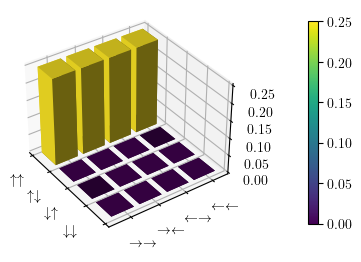
\includegraphics[width=0.6\textwidth]{imgs/wigner-desargues-2-2-s1.png}
      \caption{Función de Wigner del estado
      $\ket{\uparrow\uparrow} = \ket{0}$.}
      \label{fig:wigner-desargues-2-2-s1}
    \end{figure}
  \end{frame}

  \begin{frame}
    \frametitle{Ejemplo}

    \begin{figure}[h]
      \centering
      \scalebox{0.6}{
        %% Creator: Matplotlib, PGF backend
%%
%% To include the figure in your LaTeX document, write
%%   \input{<filename>.pgf}
%%
%% Make sure the required packages are loaded in your preamble
%%   \usepackage{pgf}
%%
%% Also ensure that all the required font packages are loaded; for instance,
%% the lmodern package is sometimes necessary when using math font.
%%   \usepackage{lmodern}
%%
%% Figures using additional raster images can only be included by \input if
%% they are in the same directory as the main LaTeX file. For loading figures
%% from other directories you can use the `import` package
%%   \usepackage{import}
%%
%% and then include the figures with
%%   \import{<path to file>}{<filename>.pgf}
%%
%% Matplotlib used the following preamble
%%   
%%   \makeatletter\@ifpackageloaded{underscore}{}{\usepackage[strings]{underscore}}\makeatother
%%
\begingroup%
\makeatletter%
\begin{pgfpicture}%
\pgfpathrectangle{\pgfpointorigin}{\pgfqpoint{4.500000in}{3.500000in}}%
\pgfusepath{use as bounding box, clip}%
\begin{pgfscope}%
\pgfsetbuttcap%
\pgfsetmiterjoin%
\definecolor{currentfill}{rgb}{1.000000,1.000000,1.000000}%
\pgfsetfillcolor{currentfill}%
\pgfsetlinewidth{0.000000pt}%
\definecolor{currentstroke}{rgb}{1.000000,1.000000,1.000000}%
\pgfsetstrokecolor{currentstroke}%
\pgfsetdash{}{0pt}%
\pgfpathmoveto{\pgfqpoint{0.000000in}{0.000000in}}%
\pgfpathlineto{\pgfqpoint{4.500000in}{0.000000in}}%
\pgfpathlineto{\pgfqpoint{4.500000in}{3.500000in}}%
\pgfpathlineto{\pgfqpoint{0.000000in}{3.500000in}}%
\pgfpathlineto{\pgfqpoint{0.000000in}{0.000000in}}%
\pgfpathclose%
\pgfusepath{fill}%
\end{pgfscope}%
\begin{pgfscope}%
\pgfsetbuttcap%
\pgfsetmiterjoin%
\definecolor{currentfill}{rgb}{1.000000,1.000000,1.000000}%
\pgfsetfillcolor{currentfill}%
\pgfsetlinewidth{0.000000pt}%
\definecolor{currentstroke}{rgb}{0.000000,0.000000,0.000000}%
\pgfsetstrokecolor{currentstroke}%
\pgfsetstrokeopacity{0.000000}%
\pgfsetdash{}{0pt}%
\pgfpathmoveto{\pgfqpoint{0.562500in}{0.599063in}}%
\pgfpathlineto{\pgfqpoint{2.829375in}{0.599063in}}%
\pgfpathlineto{\pgfqpoint{2.829375in}{2.865938in}}%
\pgfpathlineto{\pgfqpoint{0.562500in}{2.865938in}}%
\pgfpathlineto{\pgfqpoint{0.562500in}{0.599063in}}%
\pgfpathclose%
\pgfusepath{fill}%
\end{pgfscope}%
\begin{pgfscope}%
\pgfsetbuttcap%
\pgfsetmiterjoin%
\definecolor{currentfill}{rgb}{0.950000,0.950000,0.950000}%
\pgfsetfillcolor{currentfill}%
\pgfsetfillopacity{0.500000}%
\pgfsetlinewidth{1.003750pt}%
\definecolor{currentstroke}{rgb}{0.950000,0.950000,0.950000}%
\pgfsetstrokecolor{currentstroke}%
\pgfsetstrokeopacity{0.500000}%
\pgfsetdash{}{0pt}%
\pgfpathmoveto{\pgfqpoint{0.747551in}{1.430281in}}%
\pgfpathlineto{\pgfqpoint{1.890368in}{1.886175in}}%
\pgfpathlineto{\pgfqpoint{1.898416in}{2.752043in}}%
\pgfpathlineto{\pgfqpoint{0.696721in}{2.321580in}}%
\pgfusepath{stroke,fill}%
\end{pgfscope}%
\begin{pgfscope}%
\pgfsetbuttcap%
\pgfsetmiterjoin%
\definecolor{currentfill}{rgb}{0.900000,0.900000,0.900000}%
\pgfsetfillcolor{currentfill}%
\pgfsetfillopacity{0.500000}%
\pgfsetlinewidth{1.003750pt}%
\definecolor{currentstroke}{rgb}{0.900000,0.900000,0.900000}%
\pgfsetstrokecolor{currentstroke}%
\pgfsetstrokeopacity{0.500000}%
\pgfsetdash{}{0pt}%
\pgfpathmoveto{\pgfqpoint{1.890368in}{1.886175in}}%
\pgfpathlineto{\pgfqpoint{2.728721in}{1.219708in}}%
\pgfpathlineto{\pgfqpoint{2.782047in}{2.121980in}}%
\pgfpathlineto{\pgfqpoint{1.898416in}{2.752043in}}%
\pgfusepath{stroke,fill}%
\end{pgfscope}%
\begin{pgfscope}%
\pgfsetbuttcap%
\pgfsetmiterjoin%
\definecolor{currentfill}{rgb}{0.925000,0.925000,0.925000}%
\pgfsetfillcolor{currentfill}%
\pgfsetfillopacity{0.500000}%
\pgfsetlinewidth{1.003750pt}%
\definecolor{currentstroke}{rgb}{0.925000,0.925000,0.925000}%
\pgfsetstrokecolor{currentstroke}%
\pgfsetstrokeopacity{0.500000}%
\pgfsetdash{}{0pt}%
\pgfpathmoveto{\pgfqpoint{0.747551in}{1.430281in}}%
\pgfpathlineto{\pgfqpoint{1.539544in}{0.686862in}}%
\pgfpathlineto{\pgfqpoint{2.728721in}{1.219708in}}%
\pgfpathlineto{\pgfqpoint{1.890368in}{1.886175in}}%
\pgfusepath{stroke,fill}%
\end{pgfscope}%
\begin{pgfscope}%
\pgfsetrectcap%
\pgfsetroundjoin%
\pgfsetlinewidth{0.803000pt}%
\definecolor{currentstroke}{rgb}{0.000000,0.000000,0.000000}%
\pgfsetstrokecolor{currentstroke}%
\pgfsetdash{}{0pt}%
\pgfpathmoveto{\pgfqpoint{0.747551in}{1.430281in}}%
\pgfpathlineto{\pgfqpoint{1.539544in}{0.686862in}}%
\pgfusepath{stroke}%
\end{pgfscope}%
\begin{pgfscope}%
\pgfsetbuttcap%
\pgfsetroundjoin%
\pgfsetlinewidth{0.803000pt}%
\definecolor{currentstroke}{rgb}{0.690196,0.690196,0.690196}%
\pgfsetstrokecolor{currentstroke}%
\pgfsetdash{}{0pt}%
\pgfpathmoveto{\pgfqpoint{0.777375in}{1.402286in}}%
\pgfpathlineto{\pgfqpoint{1.922068in}{1.860975in}}%
\pgfpathlineto{\pgfqpoint{1.931703in}{2.728309in}}%
\pgfusepath{stroke}%
\end{pgfscope}%
\begin{pgfscope}%
\pgfsetbuttcap%
\pgfsetroundjoin%
\pgfsetlinewidth{0.803000pt}%
\definecolor{currentstroke}{rgb}{0.690196,0.690196,0.690196}%
\pgfsetstrokecolor{currentstroke}%
\pgfsetdash{}{0pt}%
\pgfpathmoveto{\pgfqpoint{0.949372in}{1.240839in}}%
\pgfpathlineto{\pgfqpoint{2.104681in}{1.715803in}}%
\pgfpathlineto{\pgfqpoint{2.123652in}{2.591442in}}%
\pgfusepath{stroke}%
\end{pgfscope}%
\begin{pgfscope}%
\pgfsetbuttcap%
\pgfsetroundjoin%
\pgfsetlinewidth{0.803000pt}%
\definecolor{currentstroke}{rgb}{0.690196,0.690196,0.690196}%
\pgfsetstrokecolor{currentstroke}%
\pgfsetdash{}{0pt}%
\pgfpathmoveto{\pgfqpoint{1.127694in}{1.073453in}}%
\pgfpathlineto{\pgfqpoint{2.293654in}{1.565575in}}%
\pgfpathlineto{\pgfqpoint{2.322627in}{2.449565in}}%
\pgfusepath{stroke}%
\end{pgfscope}%
\begin{pgfscope}%
\pgfsetbuttcap%
\pgfsetroundjoin%
\pgfsetlinewidth{0.803000pt}%
\definecolor{currentstroke}{rgb}{0.690196,0.690196,0.690196}%
\pgfsetstrokecolor{currentstroke}%
\pgfsetdash{}{0pt}%
\pgfpathmoveto{\pgfqpoint{1.312698in}{0.899796in}}%
\pgfpathlineto{\pgfqpoint{2.489324in}{1.410022in}}%
\pgfpathlineto{\pgfqpoint{2.529021in}{2.302397in}}%
\pgfusepath{stroke}%
\end{pgfscope}%
\begin{pgfscope}%
\pgfsetbuttcap%
\pgfsetroundjoin%
\pgfsetlinewidth{0.803000pt}%
\definecolor{currentstroke}{rgb}{0.690196,0.690196,0.690196}%
\pgfsetstrokecolor{currentstroke}%
\pgfsetdash{}{0pt}%
\pgfpathmoveto{\pgfqpoint{1.504765in}{0.719508in}}%
\pgfpathlineto{\pgfqpoint{2.692056in}{1.248856in}}%
\pgfpathlineto{\pgfqpoint{2.743258in}{2.149638in}}%
\pgfusepath{stroke}%
\end{pgfscope}%
\begin{pgfscope}%
\pgfsetrectcap%
\pgfsetroundjoin%
\pgfsetlinewidth{0.803000pt}%
\definecolor{currentstroke}{rgb}{0.000000,0.000000,0.000000}%
\pgfsetstrokecolor{currentstroke}%
\pgfsetdash{}{0pt}%
\pgfpathmoveto{\pgfqpoint{0.787024in}{1.406153in}}%
\pgfpathlineto{\pgfqpoint{0.758053in}{1.394544in}}%
\pgfusepath{stroke}%
\end{pgfscope}%
\begin{pgfscope}%
\definecolor{textcolor}{rgb}{0.000000,0.000000,0.000000}%
\pgfsetstrokecolor{textcolor}%
\pgfsetfillcolor{textcolor}%
\pgftext[x=0.620406in,y=1.221969in,,top]{\color{textcolor}\rmfamily\fontsize{10.000000}{12.000000}\selectfont \(\displaystyle \uparrow\uparrow\)}%
\end{pgfscope}%
\begin{pgfscope}%
\pgfsetrectcap%
\pgfsetroundjoin%
\pgfsetlinewidth{0.803000pt}%
\definecolor{currentstroke}{rgb}{0.000000,0.000000,0.000000}%
\pgfsetstrokecolor{currentstroke}%
\pgfsetdash{}{0pt}%
\pgfpathmoveto{\pgfqpoint{0.959119in}{1.244846in}}%
\pgfpathlineto{\pgfqpoint{0.929852in}{1.232814in}}%
\pgfusepath{stroke}%
\end{pgfscope}%
\begin{pgfscope}%
\definecolor{textcolor}{rgb}{0.000000,0.000000,0.000000}%
\pgfsetstrokecolor{textcolor}%
\pgfsetfillcolor{textcolor}%
\pgftext[x=0.789674in,y=1.057162in,,top]{\color{textcolor}\rmfamily\fontsize{10.000000}{12.000000}\selectfont \(\displaystyle \uparrow\downarrow\)}%
\end{pgfscope}%
\begin{pgfscope}%
\pgfsetrectcap%
\pgfsetroundjoin%
\pgfsetlinewidth{0.803000pt}%
\definecolor{currentstroke}{rgb}{0.000000,0.000000,0.000000}%
\pgfsetstrokecolor{currentstroke}%
\pgfsetdash{}{0pt}%
\pgfpathmoveto{\pgfqpoint{1.137540in}{1.077609in}}%
\pgfpathlineto{\pgfqpoint{1.107975in}{1.065130in}}%
\pgfusepath{stroke}%
\end{pgfscope}%
\begin{pgfscope}%
\definecolor{textcolor}{rgb}{0.000000,0.000000,0.000000}%
\pgfsetstrokecolor{textcolor}%
\pgfsetfillcolor{textcolor}%
\pgftext[x=0.965172in,y=0.886290in,,top]{\color{textcolor}\rmfamily\fontsize{10.000000}{12.000000}\selectfont \(\displaystyle \downarrow\uparrow\)}%
\end{pgfscope}%
\begin{pgfscope}%
\pgfsetrectcap%
\pgfsetroundjoin%
\pgfsetlinewidth{0.803000pt}%
\definecolor{currentstroke}{rgb}{0.000000,0.000000,0.000000}%
\pgfsetstrokecolor{currentstroke}%
\pgfsetdash{}{0pt}%
\pgfpathmoveto{\pgfqpoint{1.322644in}{0.904109in}}%
\pgfpathlineto{\pgfqpoint{1.292778in}{0.891158in}}%
\pgfusepath{stroke}%
\end{pgfscope}%
\begin{pgfscope}%
\definecolor{textcolor}{rgb}{0.000000,0.000000,0.000000}%
\pgfsetstrokecolor{textcolor}%
\pgfsetfillcolor{textcolor}%
\pgftext[x=1.147250in,y=0.709010in,,top]{\color{textcolor}\rmfamily\fontsize{10.000000}{12.000000}\selectfont \(\displaystyle \downarrow\downarrow\)}%
\end{pgfscope}%
\begin{pgfscope}%
\pgfsetrectcap%
\pgfsetroundjoin%
\pgfsetlinewidth{0.803000pt}%
\definecolor{currentstroke}{rgb}{0.000000,0.000000,0.000000}%
\pgfsetstrokecolor{currentstroke}%
\pgfsetdash{}{0pt}%
\pgfpathmoveto{\pgfqpoint{1.514812in}{0.723987in}}%
\pgfpathlineto{\pgfqpoint{1.484644in}{0.710537in}}%
\pgfusepath{stroke}%
\end{pgfscope}%
\begin{pgfscope}%
\pgfsetrectcap%
\pgfsetroundjoin%
\pgfsetlinewidth{0.803000pt}%
\definecolor{currentstroke}{rgb}{0.000000,0.000000,0.000000}%
\pgfsetstrokecolor{currentstroke}%
\pgfsetdash{}{0pt}%
\pgfpathmoveto{\pgfqpoint{2.728721in}{1.219708in}}%
\pgfpathlineto{\pgfqpoint{1.539544in}{0.686862in}}%
\pgfusepath{stroke}%
\end{pgfscope}%
\begin{pgfscope}%
\pgfsetbuttcap%
\pgfsetroundjoin%
\pgfsetlinewidth{0.803000pt}%
\definecolor{currentstroke}{rgb}{0.690196,0.690196,0.690196}%
\pgfsetstrokecolor{currentstroke}%
\pgfsetdash{}{0pt}%
\pgfpathmoveto{\pgfqpoint{0.921077in}{2.401947in}}%
\pgfpathlineto{\pgfqpoint{0.960455in}{1.515213in}}%
\pgfpathlineto{\pgfqpoint{1.761853in}{0.786474in}}%
\pgfusepath{stroke}%
\end{pgfscope}%
\begin{pgfscope}%
\pgfsetbuttcap%
\pgfsetroundjoin%
\pgfsetlinewidth{0.803000pt}%
\definecolor{currentstroke}{rgb}{0.690196,0.690196,0.690196}%
\pgfsetstrokecolor{currentstroke}%
\pgfsetdash{}{0pt}%
\pgfpathmoveto{\pgfqpoint{1.203262in}{2.503030in}}%
\pgfpathlineto{\pgfqpoint{1.228535in}{1.622156in}}%
\pgfpathlineto{\pgfqpoint{2.041274in}{0.911677in}}%
\pgfusepath{stroke}%
\end{pgfscope}%
\begin{pgfscope}%
\pgfsetbuttcap%
\pgfsetroundjoin%
\pgfsetlinewidth{0.803000pt}%
\definecolor{currentstroke}{rgb}{0.690196,0.690196,0.690196}%
\pgfsetstrokecolor{currentstroke}%
\pgfsetdash{}{0pt}%
\pgfpathmoveto{\pgfqpoint{1.478354in}{2.601571in}}%
\pgfpathlineto{\pgfqpoint{1.490198in}{1.726539in}}%
\pgfpathlineto{\pgfqpoint{2.313468in}{1.033642in}}%
\pgfusepath{stroke}%
\end{pgfscope}%
\begin{pgfscope}%
\pgfsetbuttcap%
\pgfsetroundjoin%
\pgfsetlinewidth{0.803000pt}%
\definecolor{currentstroke}{rgb}{0.690196,0.690196,0.690196}%
\pgfsetstrokecolor{currentstroke}%
\pgfsetdash{}{0pt}%
\pgfpathmoveto{\pgfqpoint{1.746616in}{2.697666in}}%
\pgfpathlineto{\pgfqpoint{1.745671in}{1.828452in}}%
\pgfpathlineto{\pgfqpoint{2.578712in}{1.152492in}}%
\pgfusepath{stroke}%
\end{pgfscope}%
\begin{pgfscope}%
\pgfsetrectcap%
\pgfsetroundjoin%
\pgfsetlinewidth{0.803000pt}%
\definecolor{currentstroke}{rgb}{0.000000,0.000000,0.000000}%
\pgfsetstrokecolor{currentstroke}%
\pgfsetdash{}{0pt}%
\pgfpathmoveto{\pgfqpoint{1.754918in}{0.792781in}}%
\pgfpathlineto{\pgfqpoint{1.775753in}{0.773835in}}%
\pgfusepath{stroke}%
\end{pgfscope}%
\begin{pgfscope}%
\definecolor{textcolor}{rgb}{0.000000,0.000000,0.000000}%
\pgfsetstrokecolor{textcolor}%
\pgfsetfillcolor{textcolor}%
\pgftext[x=1.879436in,y=0.560550in,,top]{\color{textcolor}\rmfamily\fontsize{10.000000}{12.000000}\selectfont \(\displaystyle \rightarrow\rightarrow\)}%
\end{pgfscope}%
\begin{pgfscope}%
\pgfsetrectcap%
\pgfsetroundjoin%
\pgfsetlinewidth{0.803000pt}%
\definecolor{currentstroke}{rgb}{0.000000,0.000000,0.000000}%
\pgfsetstrokecolor{currentstroke}%
\pgfsetdash{}{0pt}%
\pgfpathmoveto{\pgfqpoint{2.034247in}{0.917820in}}%
\pgfpathlineto{\pgfqpoint{2.055356in}{0.899367in}}%
\pgfusepath{stroke}%
\end{pgfscope}%
\begin{pgfscope}%
\definecolor{textcolor}{rgb}{0.000000,0.000000,0.000000}%
\pgfsetstrokecolor{textcolor}%
\pgfsetfillcolor{textcolor}%
\pgftext[x=2.158420in,y=0.689222in,,top]{\color{textcolor}\rmfamily\fontsize{10.000000}{12.000000}\selectfont \(\displaystyle \rightarrow\leftarrow\)}%
\end{pgfscope}%
\begin{pgfscope}%
\pgfsetrectcap%
\pgfsetroundjoin%
\pgfsetlinewidth{0.803000pt}%
\definecolor{currentstroke}{rgb}{0.000000,0.000000,0.000000}%
\pgfsetstrokecolor{currentstroke}%
\pgfsetdash{}{0pt}%
\pgfpathmoveto{\pgfqpoint{2.306357in}{1.039627in}}%
\pgfpathlineto{\pgfqpoint{2.327718in}{1.021649in}}%
\pgfusepath{stroke}%
\end{pgfscope}%
\begin{pgfscope}%
\definecolor{textcolor}{rgb}{0.000000,0.000000,0.000000}%
\pgfsetstrokecolor{textcolor}%
\pgfsetfillcolor{textcolor}%
\pgftext[x=2.430160in,y=0.814552in,,top]{\color{textcolor}\rmfamily\fontsize{10.000000}{12.000000}\selectfont \(\displaystyle \leftarrow\rightarrow\)}%
\end{pgfscope}%
\begin{pgfscope}%
\pgfsetrectcap%
\pgfsetroundjoin%
\pgfsetlinewidth{0.803000pt}%
\definecolor{currentstroke}{rgb}{0.000000,0.000000,0.000000}%
\pgfsetstrokecolor{currentstroke}%
\pgfsetdash{}{0pt}%
\pgfpathmoveto{\pgfqpoint{2.571523in}{1.158326in}}%
\pgfpathlineto{\pgfqpoint{2.593117in}{1.140803in}}%
\pgfusepath{stroke}%
\end{pgfscope}%
\begin{pgfscope}%
\definecolor{textcolor}{rgb}{0.000000,0.000000,0.000000}%
\pgfsetstrokecolor{textcolor}%
\pgfsetfillcolor{textcolor}%
\pgftext[x=2.694935in,y=0.936671in,,top]{\color{textcolor}\rmfamily\fontsize{10.000000}{12.000000}\selectfont \(\displaystyle \leftarrow\leftarrow\)}%
\end{pgfscope}%
\begin{pgfscope}%
\pgfsetrectcap%
\pgfsetroundjoin%
\pgfsetlinewidth{0.803000pt}%
\definecolor{currentstroke}{rgb}{0.000000,0.000000,0.000000}%
\pgfsetstrokecolor{currentstroke}%
\pgfsetdash{}{0pt}%
\pgfpathmoveto{\pgfqpoint{2.728721in}{1.219708in}}%
\pgfpathlineto{\pgfqpoint{2.782047in}{2.121980in}}%
\pgfusepath{stroke}%
\end{pgfscope}%
\begin{pgfscope}%
\pgfsetbuttcap%
\pgfsetroundjoin%
\pgfsetlinewidth{0.803000pt}%
\definecolor{currentstroke}{rgb}{0.690196,0.690196,0.690196}%
\pgfsetstrokecolor{currentstroke}%
\pgfsetdash{}{0pt}%
\pgfpathmoveto{\pgfqpoint{2.734629in}{1.319669in}}%
\pgfpathlineto{\pgfqpoint{1.891263in}{1.982435in}}%
\pgfpathlineto{\pgfqpoint{0.741914in}{1.529134in}}%
\pgfusepath{stroke}%
\end{pgfscope}%
\begin{pgfscope}%
\pgfsetbuttcap%
\pgfsetroundjoin%
\pgfsetlinewidth{0.803000pt}%
\definecolor{currentstroke}{rgb}{0.690196,0.690196,0.690196}%
\pgfsetstrokecolor{currentstroke}%
\pgfsetdash{}{0pt}%
\pgfpathmoveto{\pgfqpoint{2.744562in}{1.487738in}}%
\pgfpathlineto{\pgfqpoint{1.892766in}{2.144093in}}%
\pgfpathlineto{\pgfqpoint{0.732439in}{1.695280in}}%
\pgfusepath{stroke}%
\end{pgfscope}%
\begin{pgfscope}%
\pgfsetbuttcap%
\pgfsetroundjoin%
\pgfsetlinewidth{0.803000pt}%
\definecolor{currentstroke}{rgb}{0.690196,0.690196,0.690196}%
\pgfsetstrokecolor{currentstroke}%
\pgfsetdash{}{0pt}%
\pgfpathmoveto{\pgfqpoint{2.754693in}{1.659152in}}%
\pgfpathlineto{\pgfqpoint{1.894296in}{2.308729in}}%
\pgfpathlineto{\pgfqpoint{0.722779in}{1.864654in}}%
\pgfusepath{stroke}%
\end{pgfscope}%
\begin{pgfscope}%
\pgfsetbuttcap%
\pgfsetroundjoin%
\pgfsetlinewidth{0.803000pt}%
\definecolor{currentstroke}{rgb}{0.690196,0.690196,0.690196}%
\pgfsetstrokecolor{currentstroke}%
\pgfsetdash{}{0pt}%
\pgfpathmoveto{\pgfqpoint{2.765028in}{1.834012in}}%
\pgfpathlineto{\pgfqpoint{1.895855in}{2.476424in}}%
\pgfpathlineto{\pgfqpoint{0.712930in}{2.037352in}}%
\pgfusepath{stroke}%
\end{pgfscope}%
\begin{pgfscope}%
\pgfsetbuttcap%
\pgfsetroundjoin%
\pgfsetlinewidth{0.803000pt}%
\definecolor{currentstroke}{rgb}{0.690196,0.690196,0.690196}%
\pgfsetstrokecolor{currentstroke}%
\pgfsetdash{}{0pt}%
\pgfpathmoveto{\pgfqpoint{2.775572in}{2.012424in}}%
\pgfpathlineto{\pgfqpoint{1.897443in}{2.647265in}}%
\pgfpathlineto{\pgfqpoint{0.702886in}{2.213472in}}%
\pgfusepath{stroke}%
\end{pgfscope}%
\begin{pgfscope}%
\pgfsetrectcap%
\pgfsetroundjoin%
\pgfsetlinewidth{0.803000pt}%
\definecolor{currentstroke}{rgb}{0.000000,0.000000,0.000000}%
\pgfsetstrokecolor{currentstroke}%
\pgfsetdash{}{0pt}%
\pgfpathmoveto{\pgfqpoint{2.727352in}{1.325388in}}%
\pgfpathlineto{\pgfqpoint{2.749211in}{1.308210in}}%
\pgfusepath{stroke}%
\end{pgfscope}%
\begin{pgfscope}%
\definecolor{textcolor}{rgb}{0.000000,0.000000,0.000000}%
\pgfsetstrokecolor{textcolor}%
\pgfsetfillcolor{textcolor}%
\pgftext[x=3.011503in,y=1.290566in,,top]{\color{textcolor}\rmfamily\fontsize{10.000000}{12.000000}\selectfont \(\displaystyle {\ensuremath{-}0.10}\)}%
\end{pgfscope}%
\begin{pgfscope}%
\pgfsetrectcap%
\pgfsetroundjoin%
\pgfsetlinewidth{0.803000pt}%
\definecolor{currentstroke}{rgb}{0.000000,0.000000,0.000000}%
\pgfsetstrokecolor{currentstroke}%
\pgfsetdash{}{0pt}%
\pgfpathmoveto{\pgfqpoint{2.737207in}{1.493406in}}%
\pgfpathlineto{\pgfqpoint{2.759301in}{1.476381in}}%
\pgfusepath{stroke}%
\end{pgfscope}%
\begin{pgfscope}%
\definecolor{textcolor}{rgb}{0.000000,0.000000,0.000000}%
\pgfsetstrokecolor{textcolor}%
\pgfsetfillcolor{textcolor}%
\pgftext[x=3.024206in,y=1.458894in,,top]{\color{textcolor}\rmfamily\fontsize{10.000000}{12.000000}\selectfont \(\displaystyle {\ensuremath{-}0.05}\)}%
\end{pgfscope}%
\begin{pgfscope}%
\pgfsetrectcap%
\pgfsetroundjoin%
\pgfsetlinewidth{0.803000pt}%
\definecolor{currentstroke}{rgb}{0.000000,0.000000,0.000000}%
\pgfsetstrokecolor{currentstroke}%
\pgfsetdash{}{0pt}%
\pgfpathmoveto{\pgfqpoint{2.747258in}{1.664765in}}%
\pgfpathlineto{\pgfqpoint{2.769592in}{1.647904in}}%
\pgfusepath{stroke}%
\end{pgfscope}%
\begin{pgfscope}%
\definecolor{textcolor}{rgb}{0.000000,0.000000,0.000000}%
\pgfsetstrokecolor{textcolor}%
\pgfsetfillcolor{textcolor}%
\pgftext[x=3.037163in,y=1.630584in,,top]{\color{textcolor}\rmfamily\fontsize{10.000000}{12.000000}\selectfont \(\displaystyle {0.00}\)}%
\end{pgfscope}%
\begin{pgfscope}%
\pgfsetrectcap%
\pgfsetroundjoin%
\pgfsetlinewidth{0.803000pt}%
\definecolor{currentstroke}{rgb}{0.000000,0.000000,0.000000}%
\pgfsetstrokecolor{currentstroke}%
\pgfsetdash{}{0pt}%
\pgfpathmoveto{\pgfqpoint{2.757511in}{1.839568in}}%
\pgfpathlineto{\pgfqpoint{2.780090in}{1.822880in}}%
\pgfusepath{stroke}%
\end{pgfscope}%
\begin{pgfscope}%
\definecolor{textcolor}{rgb}{0.000000,0.000000,0.000000}%
\pgfsetstrokecolor{textcolor}%
\pgfsetfillcolor{textcolor}%
\pgftext[x=3.050380in,y=1.805737in,,top]{\color{textcolor}\rmfamily\fontsize{10.000000}{12.000000}\selectfont \(\displaystyle {0.05}\)}%
\end{pgfscope}%
\begin{pgfscope}%
\pgfsetrectcap%
\pgfsetroundjoin%
\pgfsetlinewidth{0.803000pt}%
\definecolor{currentstroke}{rgb}{0.000000,0.000000,0.000000}%
\pgfsetstrokecolor{currentstroke}%
\pgfsetdash{}{0pt}%
\pgfpathmoveto{\pgfqpoint{2.767973in}{2.017918in}}%
\pgfpathlineto{\pgfqpoint{2.790801in}{2.001414in}}%
\pgfusepath{stroke}%
\end{pgfscope}%
\begin{pgfscope}%
\definecolor{textcolor}{rgb}{0.000000,0.000000,0.000000}%
\pgfsetstrokecolor{textcolor}%
\pgfsetfillcolor{textcolor}%
\pgftext[x=3.063867in,y=1.984459in,,top]{\color{textcolor}\rmfamily\fontsize{10.000000}{12.000000}\selectfont \(\displaystyle {0.10}\)}%
\end{pgfscope}%
\begin{pgfscope}%
\pgfpathrectangle{\pgfqpoint{0.562500in}{0.599063in}}{\pgfqpoint{2.266875in}{2.266875in}}%
\pgfusepath{clip}%
\pgfsetbuttcap%
\pgfsetroundjoin%
\definecolor{currentfill}{rgb}{0.204703,0.003737,0.252551}%
\pgfsetfillcolor{currentfill}%
\pgfsetlinewidth{0.000000pt}%
\definecolor{currentstroke}{rgb}{0.000000,0.000000,0.000000}%
\pgfsetstrokecolor{currentstroke}%
\pgfsetdash{}{0pt}%
\pgfpathmoveto{\pgfqpoint{1.408241in}{1.649932in}}%
\pgfpathlineto{\pgfqpoint{1.550735in}{1.527960in}}%
\pgfpathlineto{\pgfqpoint{1.760286in}{1.613721in}}%
\pgfpathlineto{\pgfqpoint{1.616287in}{1.733347in}}%
\pgfpathlineto{\pgfqpoint{1.408241in}{1.649932in}}%
\pgfpathclose%
\pgfusepath{fill}%
\end{pgfscope}%
\begin{pgfscope}%
\pgfpathrectangle{\pgfqpoint{0.562500in}{0.599063in}}{\pgfqpoint{2.266875in}{2.266875in}}%
\pgfusepath{clip}%
\pgfsetbuttcap%
\pgfsetroundjoin%
\definecolor{currentfill}{rgb}{0.111252,0.002031,0.137256}%
\pgfsetfillcolor{currentfill}%
\pgfsetlinewidth{0.000000pt}%
\definecolor{currentstroke}{rgb}{0.000000,0.000000,0.000000}%
\pgfsetstrokecolor{currentstroke}%
\pgfsetdash{}{0pt}%
\pgfpathmoveto{\pgfqpoint{1.400689in}{2.062414in}}%
\pgfpathlineto{\pgfqpoint{1.408241in}{1.649932in}}%
\pgfpathlineto{\pgfqpoint{1.616287in}{1.733347in}}%
\pgfpathlineto{\pgfqpoint{1.613696in}{2.143738in}}%
\pgfpathlineto{\pgfqpoint{1.400689in}{2.062414in}}%
\pgfpathclose%
\pgfusepath{fill}%
\end{pgfscope}%
\begin{pgfscope}%
\pgfpathrectangle{\pgfqpoint{0.562500in}{0.599063in}}{\pgfqpoint{2.266875in}{2.266875in}}%
\pgfusepath{clip}%
\pgfsetbuttcap%
\pgfsetroundjoin%
\definecolor{currentfill}{rgb}{0.235854,0.004305,0.290983}%
\pgfsetfillcolor{currentfill}%
\pgfsetlinewidth{0.000000pt}%
\definecolor{currentstroke}{rgb}{0.000000,0.000000,0.000000}%
\pgfsetstrokecolor{currentstroke}%
\pgfsetdash{}{0pt}%
\pgfpathmoveto{\pgfqpoint{1.613696in}{2.143738in}}%
\pgfpathlineto{\pgfqpoint{1.616287in}{1.733347in}}%
\pgfpathlineto{\pgfqpoint{1.760286in}{1.613721in}}%
\pgfpathlineto{\pgfqpoint{1.761089in}{2.027100in}}%
\pgfpathlineto{\pgfqpoint{1.613696in}{2.143738in}}%
\pgfpathclose%
\pgfusepath{fill}%
\end{pgfscope}%
\begin{pgfscope}%
\pgfpathrectangle{\pgfqpoint{0.562500in}{0.599063in}}{\pgfqpoint{2.266875in}{2.266875in}}%
\pgfusepath{clip}%
\pgfsetbuttcap%
\pgfsetroundjoin%
\definecolor{currentfill}{rgb}{0.529732,0.483284,0.076766}%
\pgfsetfillcolor{currentfill}%
\pgfsetlinewidth{0.000000pt}%
\definecolor{currentstroke}{rgb}{0.000000,0.000000,0.000000}%
\pgfsetstrokecolor{currentstroke}%
\pgfsetdash{}{0pt}%
\pgfpathmoveto{\pgfqpoint{1.666296in}{2.163820in}}%
\pgfpathlineto{\pgfqpoint{1.874144in}{2.243174in}}%
\pgfpathlineto{\pgfqpoint{2.023383in}{2.129368in}}%
\pgfpathlineto{\pgfqpoint{1.814069in}{2.047757in}}%
\pgfpathlineto{\pgfqpoint{1.666296in}{2.163820in}}%
\pgfpathclose%
\pgfusepath{fill}%
\end{pgfscope}%
\begin{pgfscope}%
\pgfpathrectangle{\pgfqpoint{0.562500in}{0.599063in}}{\pgfqpoint{2.266875in}{2.266875in}}%
\pgfusepath{clip}%
\pgfsetbuttcap%
\pgfsetroundjoin%
\definecolor{currentfill}{rgb}{0.877369,0.800439,0.127143}%
\pgfsetfillcolor{currentfill}%
\pgfsetlinewidth{0.000000pt}%
\definecolor{currentstroke}{rgb}{0.000000,0.000000,0.000000}%
\pgfsetstrokecolor{currentstroke}%
\pgfsetdash{}{0pt}%
\pgfpathmoveto{\pgfqpoint{1.666296in}{2.163820in}}%
\pgfpathlineto{\pgfqpoint{1.664850in}{2.593360in}}%
\pgfpathlineto{\pgfqpoint{1.877650in}{2.670333in}}%
\pgfpathlineto{\pgfqpoint{1.874144in}{2.243174in}}%
\pgfpathlineto{\pgfqpoint{1.666296in}{2.163820in}}%
\pgfpathclose%
\pgfusepath{fill}%
\end{pgfscope}%
\begin{pgfscope}%
\pgfpathrectangle{\pgfqpoint{0.562500in}{0.599063in}}{\pgfqpoint{2.266875in}{2.266875in}}%
\pgfusepath{clip}%
\pgfsetbuttcap%
\pgfsetroundjoin%
\definecolor{currentfill}{rgb}{0.111252,0.002031,0.137256}%
\pgfsetfillcolor{currentfill}%
\pgfsetlinewidth{0.000000pt}%
\definecolor{currentstroke}{rgb}{0.000000,0.000000,0.000000}%
\pgfsetstrokecolor{currentstroke}%
\pgfsetdash{}{0pt}%
\pgfpathmoveto{\pgfqpoint{1.400689in}{2.062414in}}%
\pgfpathlineto{\pgfqpoint{1.546504in}{1.943434in}}%
\pgfpathlineto{\pgfqpoint{1.550735in}{1.527960in}}%
\pgfpathlineto{\pgfqpoint{1.408241in}{1.649932in}}%
\pgfpathlineto{\pgfqpoint{1.400689in}{2.062414in}}%
\pgfpathclose%
\pgfusepath{fill}%
\end{pgfscope}%
\begin{pgfscope}%
\pgfpathrectangle{\pgfqpoint{0.562500in}{0.599063in}}{\pgfqpoint{2.266875in}{2.266875in}}%
\pgfusepath{clip}%
\pgfsetbuttcap%
\pgfsetroundjoin%
\definecolor{currentfill}{rgb}{0.413853,0.377565,0.059973}%
\pgfsetfillcolor{currentfill}%
\pgfsetlinewidth{0.000000pt}%
\definecolor{currentstroke}{rgb}{0.000000,0.000000,0.000000}%
\pgfsetstrokecolor{currentstroke}%
\pgfsetdash{}{0pt}%
\pgfpathmoveto{\pgfqpoint{1.874144in}{2.243174in}}%
\pgfpathlineto{\pgfqpoint{1.877650in}{2.670333in}}%
\pgfpathlineto{\pgfqpoint{2.030536in}{2.559930in}}%
\pgfpathlineto{\pgfqpoint{2.023383in}{2.129368in}}%
\pgfpathlineto{\pgfqpoint{1.874144in}{2.243174in}}%
\pgfpathclose%
\pgfusepath{fill}%
\end{pgfscope}%
\begin{pgfscope}%
\pgfpathrectangle{\pgfqpoint{0.562500in}{0.599063in}}{\pgfqpoint{2.266875in}{2.266875in}}%
\pgfusepath{clip}%
\pgfsetbuttcap%
\pgfsetroundjoin%
\definecolor{currentfill}{rgb}{0.235854,0.004305,0.290983}%
\pgfsetfillcolor{currentfill}%
\pgfsetlinewidth{0.000000pt}%
\definecolor{currentstroke}{rgb}{0.000000,0.000000,0.000000}%
\pgfsetstrokecolor{currentstroke}%
\pgfsetdash{}{0pt}%
\pgfpathmoveto{\pgfqpoint{1.546504in}{1.943434in}}%
\pgfpathlineto{\pgfqpoint{1.761089in}{2.027100in}}%
\pgfpathlineto{\pgfqpoint{1.760286in}{1.613721in}}%
\pgfpathlineto{\pgfqpoint{1.550735in}{1.527960in}}%
\pgfpathlineto{\pgfqpoint{1.546504in}{1.943434in}}%
\pgfpathclose%
\pgfusepath{fill}%
\end{pgfscope}%
\begin{pgfscope}%
\pgfpathrectangle{\pgfqpoint{0.562500in}{0.599063in}}{\pgfqpoint{2.266875in}{2.266875in}}%
\pgfusepath{clip}%
\pgfsetbuttcap%
\pgfsetroundjoin%
\definecolor{currentfill}{rgb}{0.142402,0.002599,0.175688}%
\pgfsetfillcolor{currentfill}%
\pgfsetlinewidth{0.000000pt}%
\definecolor{currentstroke}{rgb}{0.000000,0.000000,0.000000}%
\pgfsetstrokecolor{currentstroke}%
\pgfsetdash{}{0pt}%
\pgfpathmoveto{\pgfqpoint{1.400689in}{2.062414in}}%
\pgfpathlineto{\pgfqpoint{1.613696in}{2.143738in}}%
\pgfpathlineto{\pgfqpoint{1.761089in}{2.027100in}}%
\pgfpathlineto{\pgfqpoint{1.546504in}{1.943434in}}%
\pgfpathlineto{\pgfqpoint{1.400689in}{2.062414in}}%
\pgfpathclose%
\pgfusepath{fill}%
\end{pgfscope}%
\begin{pgfscope}%
\pgfpathrectangle{\pgfqpoint{0.562500in}{0.599063in}}{\pgfqpoint{2.266875in}{2.266875in}}%
\pgfusepath{clip}%
\pgfsetbuttcap%
\pgfsetroundjoin%
\definecolor{currentfill}{rgb}{0.204703,0.003737,0.252551}%
\pgfsetfillcolor{currentfill}%
\pgfsetlinewidth{0.000000pt}%
\definecolor{currentstroke}{rgb}{0.000000,0.000000,0.000000}%
\pgfsetstrokecolor{currentstroke}%
\pgfsetdash{}{0pt}%
\pgfpathmoveto{\pgfqpoint{0.870050in}{1.434146in}}%
\pgfpathlineto{\pgfqpoint{1.008391in}{1.305999in}}%
\pgfpathlineto{\pgfqpoint{1.228574in}{1.396111in}}%
\pgfpathlineto{\pgfqpoint{1.088501in}{1.521733in}}%
\pgfpathlineto{\pgfqpoint{0.870050in}{1.434146in}}%
\pgfpathclose%
\pgfusepath{fill}%
\end{pgfscope}%
\begin{pgfscope}%
\pgfpathrectangle{\pgfqpoint{0.562500in}{0.599063in}}{\pgfqpoint{2.266875in}{2.266875in}}%
\pgfusepath{clip}%
\pgfsetbuttcap%
\pgfsetroundjoin%
\definecolor{currentfill}{rgb}{0.877369,0.800439,0.127143}%
\pgfsetfillcolor{currentfill}%
\pgfsetlinewidth{0.000000pt}%
\definecolor{currentstroke}{rgb}{0.000000,0.000000,0.000000}%
\pgfsetstrokecolor{currentstroke}%
\pgfsetdash{}{0pt}%
\pgfpathmoveto{\pgfqpoint{1.666296in}{2.163820in}}%
\pgfpathlineto{\pgfqpoint{1.814069in}{2.047757in}}%
\pgfpathlineto{\pgfqpoint{1.816199in}{2.480714in}}%
\pgfpathlineto{\pgfqpoint{1.664850in}{2.593360in}}%
\pgfpathlineto{\pgfqpoint{1.666296in}{2.163820in}}%
\pgfpathclose%
\pgfusepath{fill}%
\end{pgfscope}%
\begin{pgfscope}%
\pgfpathrectangle{\pgfqpoint{0.562500in}{0.599063in}}{\pgfqpoint{2.266875in}{2.266875in}}%
\pgfusepath{clip}%
\pgfsetbuttcap%
\pgfsetroundjoin%
\definecolor{currentfill}{rgb}{0.529732,0.483284,0.076766}%
\pgfsetfillcolor{currentfill}%
\pgfsetlinewidth{0.000000pt}%
\definecolor{currentstroke}{rgb}{0.000000,0.000000,0.000000}%
\pgfsetstrokecolor{currentstroke}%
\pgfsetdash{}{0pt}%
\pgfpathmoveto{\pgfqpoint{1.851670in}{2.018225in}}%
\pgfpathlineto{\pgfqpoint{2.061350in}{2.100415in}}%
\pgfpathlineto{\pgfqpoint{2.215935in}{1.982532in}}%
\pgfpathlineto{\pgfqpoint{2.004789in}{1.897962in}}%
\pgfpathlineto{\pgfqpoint{1.851670in}{2.018225in}}%
\pgfpathclose%
\pgfusepath{fill}%
\end{pgfscope}%
\begin{pgfscope}%
\pgfpathrectangle{\pgfqpoint{0.562500in}{0.599063in}}{\pgfqpoint{2.266875in}{2.266875in}}%
\pgfusepath{clip}%
\pgfsetbuttcap%
\pgfsetroundjoin%
\definecolor{currentfill}{rgb}{0.111252,0.002031,0.137256}%
\pgfsetfillcolor{currentfill}%
\pgfsetlinewidth{0.000000pt}%
\definecolor{currentstroke}{rgb}{0.000000,0.000000,0.000000}%
\pgfsetstrokecolor{currentstroke}%
\pgfsetdash{}{0pt}%
\pgfpathmoveto{\pgfqpoint{0.849213in}{1.851867in}}%
\pgfpathlineto{\pgfqpoint{0.870050in}{1.434146in}}%
\pgfpathlineto{\pgfqpoint{1.088501in}{1.521733in}}%
\pgfpathlineto{\pgfqpoint{1.073135in}{1.937358in}}%
\pgfpathlineto{\pgfqpoint{0.849213in}{1.851867in}}%
\pgfpathclose%
\pgfusepath{fill}%
\end{pgfscope}%
\begin{pgfscope}%
\pgfpathrectangle{\pgfqpoint{0.562500in}{0.599063in}}{\pgfqpoint{2.266875in}{2.266875in}}%
\pgfusepath{clip}%
\pgfsetbuttcap%
\pgfsetroundjoin%
\definecolor{currentfill}{rgb}{0.413853,0.377565,0.059973}%
\pgfsetfillcolor{currentfill}%
\pgfsetlinewidth{0.000000pt}%
\definecolor{currentstroke}{rgb}{0.000000,0.000000,0.000000}%
\pgfsetstrokecolor{currentstroke}%
\pgfsetdash{}{0pt}%
\pgfpathmoveto{\pgfqpoint{1.814069in}{2.047757in}}%
\pgfpathlineto{\pgfqpoint{2.023383in}{2.129368in}}%
\pgfpathlineto{\pgfqpoint{2.030536in}{2.559930in}}%
\pgfpathlineto{\pgfqpoint{1.816199in}{2.480714in}}%
\pgfpathlineto{\pgfqpoint{1.814069in}{2.047757in}}%
\pgfpathclose%
\pgfusepath{fill}%
\end{pgfscope}%
\begin{pgfscope}%
\pgfpathrectangle{\pgfqpoint{0.562500in}{0.599063in}}{\pgfqpoint{2.266875in}{2.266875in}}%
\pgfusepath{clip}%
\pgfsetbuttcap%
\pgfsetroundjoin%
\definecolor{currentfill}{rgb}{0.235854,0.004305,0.290983}%
\pgfsetfillcolor{currentfill}%
\pgfsetlinewidth{0.000000pt}%
\definecolor{currentstroke}{rgb}{0.000000,0.000000,0.000000}%
\pgfsetstrokecolor{currentstroke}%
\pgfsetdash{}{0pt}%
\pgfpathmoveto{\pgfqpoint{1.073135in}{1.937358in}}%
\pgfpathlineto{\pgfqpoint{1.088501in}{1.521733in}}%
\pgfpathlineto{\pgfqpoint{1.228574in}{1.396111in}}%
\pgfpathlineto{\pgfqpoint{1.216405in}{1.814730in}}%
\pgfpathlineto{\pgfqpoint{1.073135in}{1.937358in}}%
\pgfpathclose%
\pgfusepath{fill}%
\end{pgfscope}%
\begin{pgfscope}%
\pgfpathrectangle{\pgfqpoint{0.562500in}{0.599063in}}{\pgfqpoint{2.266875in}{2.266875in}}%
\pgfusepath{clip}%
\pgfsetbuttcap%
\pgfsetroundjoin%
\definecolor{currentfill}{rgb}{0.877369,0.800439,0.127143}%
\pgfsetfillcolor{currentfill}%
\pgfsetlinewidth{0.000000pt}%
\definecolor{currentstroke}{rgb}{0.000000,0.000000,0.000000}%
\pgfsetstrokecolor{currentstroke}%
\pgfsetdash{}{0pt}%
\pgfpathmoveto{\pgfqpoint{1.851670in}{2.018225in}}%
\pgfpathlineto{\pgfqpoint{1.854726in}{2.452039in}}%
\pgfpathlineto{\pgfqpoint{2.069448in}{2.531831in}}%
\pgfpathlineto{\pgfqpoint{2.061350in}{2.100415in}}%
\pgfpathlineto{\pgfqpoint{1.851670in}{2.018225in}}%
\pgfpathclose%
\pgfusepath{fill}%
\end{pgfscope}%
\begin{pgfscope}%
\pgfpathrectangle{\pgfqpoint{0.562500in}{0.599063in}}{\pgfqpoint{2.266875in}{2.266875in}}%
\pgfusepath{clip}%
\pgfsetbuttcap%
\pgfsetroundjoin%
\definecolor{currentfill}{rgb}{0.761490,0.694720,0.110351}%
\pgfsetfillcolor{currentfill}%
\pgfsetlinewidth{0.000000pt}%
\definecolor{currentstroke}{rgb}{0.000000,0.000000,0.000000}%
\pgfsetstrokecolor{currentstroke}%
\pgfsetdash{}{0pt}%
\pgfpathmoveto{\pgfqpoint{1.664850in}{2.593360in}}%
\pgfpathlineto{\pgfqpoint{1.816199in}{2.480714in}}%
\pgfpathlineto{\pgfqpoint{2.030536in}{2.559930in}}%
\pgfpathlineto{\pgfqpoint{1.877650in}{2.670333in}}%
\pgfpathlineto{\pgfqpoint{1.664850in}{2.593360in}}%
\pgfpathclose%
\pgfusepath{fill}%
\end{pgfscope}%
\begin{pgfscope}%
\pgfpathrectangle{\pgfqpoint{0.562500in}{0.599063in}}{\pgfqpoint{2.266875in}{2.266875in}}%
\pgfusepath{clip}%
\pgfsetbuttcap%
\pgfsetroundjoin%
\definecolor{currentfill}{rgb}{0.413853,0.377565,0.059973}%
\pgfsetfillcolor{currentfill}%
\pgfsetlinewidth{0.000000pt}%
\definecolor{currentstroke}{rgb}{0.000000,0.000000,0.000000}%
\pgfsetstrokecolor{currentstroke}%
\pgfsetdash{}{0pt}%
\pgfpathmoveto{\pgfqpoint{2.061350in}{2.100415in}}%
\pgfpathlineto{\pgfqpoint{2.069448in}{2.531831in}}%
\pgfpathlineto{\pgfqpoint{2.227945in}{2.417376in}}%
\pgfpathlineto{\pgfqpoint{2.215935in}{1.982532in}}%
\pgfpathlineto{\pgfqpoint{2.061350in}{2.100415in}}%
\pgfpathclose%
\pgfusepath{fill}%
\end{pgfscope}%
\begin{pgfscope}%
\pgfpathrectangle{\pgfqpoint{0.562500in}{0.599063in}}{\pgfqpoint{2.266875in}{2.266875in}}%
\pgfusepath{clip}%
\pgfsetbuttcap%
\pgfsetroundjoin%
\definecolor{currentfill}{rgb}{0.529732,0.483284,0.076766}%
\pgfsetfillcolor{currentfill}%
\pgfsetlinewidth{0.000000pt}%
\definecolor{currentstroke}{rgb}{0.000000,0.000000,0.000000}%
\pgfsetstrokecolor{currentstroke}%
\pgfsetdash{}{0pt}%
\pgfpathmoveto{\pgfqpoint{1.128412in}{1.958462in}}%
\pgfpathlineto{\pgfqpoint{1.346775in}{2.041830in}}%
\pgfpathlineto{\pgfqpoint{1.492181in}{1.922254in}}%
\pgfpathlineto{\pgfqpoint{1.272123in}{1.836454in}}%
\pgfpathlineto{\pgfqpoint{1.128412in}{1.958462in}}%
\pgfpathclose%
\pgfusepath{fill}%
\end{pgfscope}%
\begin{pgfscope}%
\pgfpathrectangle{\pgfqpoint{0.562500in}{0.599063in}}{\pgfqpoint{2.266875in}{2.266875in}}%
\pgfusepath{clip}%
\pgfsetbuttcap%
\pgfsetroundjoin%
\definecolor{currentfill}{rgb}{0.877369,0.800439,0.127143}%
\pgfsetfillcolor{currentfill}%
\pgfsetlinewidth{0.000000pt}%
\definecolor{currentstroke}{rgb}{0.000000,0.000000,0.000000}%
\pgfsetstrokecolor{currentstroke}%
\pgfsetdash{}{0pt}%
\pgfpathmoveto{\pgfqpoint{1.128412in}{1.958462in}}%
\pgfpathlineto{\pgfqpoint{1.113690in}{2.393997in}}%
\pgfpathlineto{\pgfqpoint{1.337522in}{2.474960in}}%
\pgfpathlineto{\pgfqpoint{1.346775in}{2.041830in}}%
\pgfpathlineto{\pgfqpoint{1.128412in}{1.958462in}}%
\pgfpathclose%
\pgfusepath{fill}%
\end{pgfscope}%
\begin{pgfscope}%
\pgfpathrectangle{\pgfqpoint{0.562500in}{0.599063in}}{\pgfqpoint{2.266875in}{2.266875in}}%
\pgfusepath{clip}%
\pgfsetbuttcap%
\pgfsetroundjoin%
\definecolor{currentfill}{rgb}{0.529732,0.483284,0.076766}%
\pgfsetfillcolor{currentfill}%
\pgfsetlinewidth{0.000000pt}%
\definecolor{currentstroke}{rgb}{0.000000,0.000000,0.000000}%
\pgfsetstrokecolor{currentstroke}%
\pgfsetdash{}{0pt}%
\pgfpathmoveto{\pgfqpoint{1.583614in}{1.913153in}}%
\pgfpathlineto{\pgfqpoint{1.798595in}{1.997420in}}%
\pgfpathlineto{\pgfqpoint{1.951334in}{1.876551in}}%
\pgfpathlineto{\pgfqpoint{1.734773in}{1.789813in}}%
\pgfpathlineto{\pgfqpoint{1.583614in}{1.913153in}}%
\pgfpathclose%
\pgfusepath{fill}%
\end{pgfscope}%
\begin{pgfscope}%
\pgfpathrectangle{\pgfqpoint{0.562500in}{0.599063in}}{\pgfqpoint{2.266875in}{2.266875in}}%
\pgfusepath{clip}%
\pgfsetbuttcap%
\pgfsetroundjoin%
\definecolor{currentfill}{rgb}{0.111252,0.002031,0.137256}%
\pgfsetfillcolor{currentfill}%
\pgfsetlinewidth{0.000000pt}%
\definecolor{currentstroke}{rgb}{0.000000,0.000000,0.000000}%
\pgfsetstrokecolor{currentstroke}%
\pgfsetdash{}{0pt}%
\pgfpathmoveto{\pgfqpoint{0.849213in}{1.851867in}}%
\pgfpathlineto{\pgfqpoint{0.990662in}{1.726714in}}%
\pgfpathlineto{\pgfqpoint{1.008391in}{1.305999in}}%
\pgfpathlineto{\pgfqpoint{0.870050in}{1.434146in}}%
\pgfpathlineto{\pgfqpoint{0.849213in}{1.851867in}}%
\pgfpathclose%
\pgfusepath{fill}%
\end{pgfscope}%
\begin{pgfscope}%
\pgfpathrectangle{\pgfqpoint{0.562500in}{0.599063in}}{\pgfqpoint{2.266875in}{2.266875in}}%
\pgfusepath{clip}%
\pgfsetbuttcap%
\pgfsetroundjoin%
\definecolor{currentfill}{rgb}{0.413853,0.377565,0.059973}%
\pgfsetfillcolor{currentfill}%
\pgfsetlinewidth{0.000000pt}%
\definecolor{currentstroke}{rgb}{0.000000,0.000000,0.000000}%
\pgfsetstrokecolor{currentstroke}%
\pgfsetdash{}{0pt}%
\pgfpathmoveto{\pgfqpoint{1.346775in}{2.041830in}}%
\pgfpathlineto{\pgfqpoint{1.337522in}{2.474960in}}%
\pgfpathlineto{\pgfqpoint{1.486386in}{2.358821in}}%
\pgfpathlineto{\pgfqpoint{1.492181in}{1.922254in}}%
\pgfpathlineto{\pgfqpoint{1.346775in}{2.041830in}}%
\pgfpathclose%
\pgfusepath{fill}%
\end{pgfscope}%
\begin{pgfscope}%
\pgfpathrectangle{\pgfqpoint{0.562500in}{0.599063in}}{\pgfqpoint{2.266875in}{2.266875in}}%
\pgfusepath{clip}%
\pgfsetbuttcap%
\pgfsetroundjoin%
\definecolor{currentfill}{rgb}{0.235854,0.004305,0.290983}%
\pgfsetfillcolor{currentfill}%
\pgfsetlinewidth{0.000000pt}%
\definecolor{currentstroke}{rgb}{0.000000,0.000000,0.000000}%
\pgfsetstrokecolor{currentstroke}%
\pgfsetdash{}{0pt}%
\pgfpathmoveto{\pgfqpoint{0.990662in}{1.726714in}}%
\pgfpathlineto{\pgfqpoint{1.216405in}{1.814730in}}%
\pgfpathlineto{\pgfqpoint{1.228574in}{1.396111in}}%
\pgfpathlineto{\pgfqpoint{1.008391in}{1.305999in}}%
\pgfpathlineto{\pgfqpoint{0.990662in}{1.726714in}}%
\pgfpathclose%
\pgfusepath{fill}%
\end{pgfscope}%
\begin{pgfscope}%
\pgfpathrectangle{\pgfqpoint{0.562500in}{0.599063in}}{\pgfqpoint{2.266875in}{2.266875in}}%
\pgfusepath{clip}%
\pgfsetbuttcap%
\pgfsetroundjoin%
\definecolor{currentfill}{rgb}{0.877369,0.800439,0.127143}%
\pgfsetfillcolor{currentfill}%
\pgfsetlinewidth{0.000000pt}%
\definecolor{currentstroke}{rgb}{0.000000,0.000000,0.000000}%
\pgfsetstrokecolor{currentstroke}%
\pgfsetdash{}{0pt}%
\pgfpathmoveto{\pgfqpoint{1.851670in}{2.018225in}}%
\pgfpathlineto{\pgfqpoint{2.004789in}{1.897962in}}%
\pgfpathlineto{\pgfqpoint{2.011688in}{2.335217in}}%
\pgfpathlineto{\pgfqpoint{1.854726in}{2.452039in}}%
\pgfpathlineto{\pgfqpoint{1.851670in}{2.018225in}}%
\pgfpathclose%
\pgfusepath{fill}%
\end{pgfscope}%
\begin{pgfscope}%
\pgfpathrectangle{\pgfqpoint{0.562500in}{0.599063in}}{\pgfqpoint{2.266875in}{2.266875in}}%
\pgfusepath{clip}%
\pgfsetbuttcap%
\pgfsetroundjoin%
\definecolor{currentfill}{rgb}{0.877369,0.800439,0.127143}%
\pgfsetfillcolor{currentfill}%
\pgfsetlinewidth{0.000000pt}%
\definecolor{currentstroke}{rgb}{0.000000,0.000000,0.000000}%
\pgfsetstrokecolor{currentstroke}%
\pgfsetdash{}{0pt}%
\pgfpathmoveto{\pgfqpoint{1.583614in}{1.913153in}}%
\pgfpathlineto{\pgfqpoint{1.580076in}{2.349978in}}%
\pgfpathlineto{\pgfqpoint{1.800359in}{2.431836in}}%
\pgfpathlineto{\pgfqpoint{1.798595in}{1.997420in}}%
\pgfpathlineto{\pgfqpoint{1.583614in}{1.913153in}}%
\pgfpathclose%
\pgfusepath{fill}%
\end{pgfscope}%
\begin{pgfscope}%
\pgfpathrectangle{\pgfqpoint{0.562500in}{0.599063in}}{\pgfqpoint{2.266875in}{2.266875in}}%
\pgfusepath{clip}%
\pgfsetbuttcap%
\pgfsetroundjoin%
\definecolor{currentfill}{rgb}{0.529732,0.483284,0.076766}%
\pgfsetfillcolor{currentfill}%
\pgfsetlinewidth{0.000000pt}%
\definecolor{currentstroke}{rgb}{0.000000,0.000000,0.000000}%
\pgfsetstrokecolor{currentstroke}%
\pgfsetdash{}{0pt}%
\pgfpathmoveto{\pgfqpoint{2.043763in}{1.867351in}}%
\pgfpathlineto{\pgfqpoint{2.255275in}{1.952532in}}%
\pgfpathlineto{\pgfqpoint{2.415497in}{1.830350in}}%
\pgfpathlineto{\pgfqpoint{2.202524in}{1.742658in}}%
\pgfpathlineto{\pgfqpoint{2.043763in}{1.867351in}}%
\pgfpathclose%
\pgfusepath{fill}%
\end{pgfscope}%
\begin{pgfscope}%
\pgfpathrectangle{\pgfqpoint{0.562500in}{0.599063in}}{\pgfqpoint{2.266875in}{2.266875in}}%
\pgfusepath{clip}%
\pgfsetbuttcap%
\pgfsetroundjoin%
\definecolor{currentfill}{rgb}{0.413853,0.377565,0.059973}%
\pgfsetfillcolor{currentfill}%
\pgfsetlinewidth{0.000000pt}%
\definecolor{currentstroke}{rgb}{0.000000,0.000000,0.000000}%
\pgfsetstrokecolor{currentstroke}%
\pgfsetdash{}{0pt}%
\pgfpathmoveto{\pgfqpoint{2.004789in}{1.897962in}}%
\pgfpathlineto{\pgfqpoint{2.215935in}{1.982532in}}%
\pgfpathlineto{\pgfqpoint{2.227945in}{2.417376in}}%
\pgfpathlineto{\pgfqpoint{2.011688in}{2.335217in}}%
\pgfpathlineto{\pgfqpoint{2.004789in}{1.897962in}}%
\pgfpathclose%
\pgfusepath{fill}%
\end{pgfscope}%
\begin{pgfscope}%
\pgfpathrectangle{\pgfqpoint{0.562500in}{0.599063in}}{\pgfqpoint{2.266875in}{2.266875in}}%
\pgfusepath{clip}%
\pgfsetbuttcap%
\pgfsetroundjoin%
\definecolor{currentfill}{rgb}{0.413853,0.377565,0.059973}%
\pgfsetfillcolor{currentfill}%
\pgfsetlinewidth{0.000000pt}%
\definecolor{currentstroke}{rgb}{0.000000,0.000000,0.000000}%
\pgfsetstrokecolor{currentstroke}%
\pgfsetdash{}{0pt}%
\pgfpathmoveto{\pgfqpoint{1.798595in}{1.997420in}}%
\pgfpathlineto{\pgfqpoint{1.800359in}{2.431836in}}%
\pgfpathlineto{\pgfqpoint{1.956921in}{2.314411in}}%
\pgfpathlineto{\pgfqpoint{1.951334in}{1.876551in}}%
\pgfpathlineto{\pgfqpoint{1.798595in}{1.997420in}}%
\pgfpathclose%
\pgfusepath{fill}%
\end{pgfscope}%
\begin{pgfscope}%
\pgfpathrectangle{\pgfqpoint{0.562500in}{0.599063in}}{\pgfqpoint{2.266875in}{2.266875in}}%
\pgfusepath{clip}%
\pgfsetbuttcap%
\pgfsetroundjoin%
\definecolor{currentfill}{rgb}{0.142402,0.002599,0.175688}%
\pgfsetfillcolor{currentfill}%
\pgfsetlinewidth{0.000000pt}%
\definecolor{currentstroke}{rgb}{0.000000,0.000000,0.000000}%
\pgfsetstrokecolor{currentstroke}%
\pgfsetdash{}{0pt}%
\pgfpathmoveto{\pgfqpoint{0.849213in}{1.851867in}}%
\pgfpathlineto{\pgfqpoint{1.073135in}{1.937358in}}%
\pgfpathlineto{\pgfqpoint{1.216405in}{1.814730in}}%
\pgfpathlineto{\pgfqpoint{0.990662in}{1.726714in}}%
\pgfpathlineto{\pgfqpoint{0.849213in}{1.851867in}}%
\pgfpathclose%
\pgfusepath{fill}%
\end{pgfscope}%
\begin{pgfscope}%
\pgfpathrectangle{\pgfqpoint{0.562500in}{0.599063in}}{\pgfqpoint{2.266875in}{2.266875in}}%
\pgfusepath{clip}%
\pgfsetbuttcap%
\pgfsetroundjoin%
\definecolor{currentfill}{rgb}{0.877369,0.800439,0.127143}%
\pgfsetfillcolor{currentfill}%
\pgfsetlinewidth{0.000000pt}%
\definecolor{currentstroke}{rgb}{0.000000,0.000000,0.000000}%
\pgfsetstrokecolor{currentstroke}%
\pgfsetdash{}{0pt}%
\pgfpathmoveto{\pgfqpoint{2.043763in}{1.867351in}}%
\pgfpathlineto{\pgfqpoint{2.051657in}{2.305469in}}%
\pgfpathlineto{\pgfqpoint{2.268298in}{2.388237in}}%
\pgfpathlineto{\pgfqpoint{2.255275in}{1.952532in}}%
\pgfpathlineto{\pgfqpoint{2.043763in}{1.867351in}}%
\pgfpathclose%
\pgfusepath{fill}%
\end{pgfscope}%
\begin{pgfscope}%
\pgfpathrectangle{\pgfqpoint{0.562500in}{0.599063in}}{\pgfqpoint{2.266875in}{2.266875in}}%
\pgfusepath{clip}%
\pgfsetbuttcap%
\pgfsetroundjoin%
\definecolor{currentfill}{rgb}{0.761490,0.694720,0.110351}%
\pgfsetfillcolor{currentfill}%
\pgfsetlinewidth{0.000000pt}%
\definecolor{currentstroke}{rgb}{0.000000,0.000000,0.000000}%
\pgfsetstrokecolor{currentstroke}%
\pgfsetdash{}{0pt}%
\pgfpathmoveto{\pgfqpoint{1.854726in}{2.452039in}}%
\pgfpathlineto{\pgfqpoint{2.011688in}{2.335217in}}%
\pgfpathlineto{\pgfqpoint{2.227945in}{2.417376in}}%
\pgfpathlineto{\pgfqpoint{2.069448in}{2.531831in}}%
\pgfpathlineto{\pgfqpoint{1.854726in}{2.452039in}}%
\pgfpathclose%
\pgfusepath{fill}%
\end{pgfscope}%
\begin{pgfscope}%
\pgfpathrectangle{\pgfqpoint{0.562500in}{0.599063in}}{\pgfqpoint{2.266875in}{2.266875in}}%
\pgfusepath{clip}%
\pgfsetbuttcap%
\pgfsetroundjoin%
\definecolor{currentfill}{rgb}{0.877369,0.800439,0.127143}%
\pgfsetfillcolor{currentfill}%
\pgfsetlinewidth{0.000000pt}%
\definecolor{currentstroke}{rgb}{0.000000,0.000000,0.000000}%
\pgfsetstrokecolor{currentstroke}%
\pgfsetdash{}{0pt}%
\pgfpathmoveto{\pgfqpoint{1.128412in}{1.958462in}}%
\pgfpathlineto{\pgfqpoint{1.272123in}{1.836454in}}%
\pgfpathlineto{\pgfqpoint{1.260770in}{2.275437in}}%
\pgfpathlineto{\pgfqpoint{1.113690in}{2.393997in}}%
\pgfpathlineto{\pgfqpoint{1.128412in}{1.958462in}}%
\pgfpathclose%
\pgfusepath{fill}%
\end{pgfscope}%
\begin{pgfscope}%
\pgfpathrectangle{\pgfqpoint{0.562500in}{0.599063in}}{\pgfqpoint{2.266875in}{2.266875in}}%
\pgfusepath{clip}%
\pgfsetbuttcap%
\pgfsetroundjoin%
\definecolor{currentfill}{rgb}{0.204703,0.003737,0.252551}%
\pgfsetfillcolor{currentfill}%
\pgfsetlinewidth{0.000000pt}%
\definecolor{currentstroke}{rgb}{0.000000,0.000000,0.000000}%
\pgfsetstrokecolor{currentstroke}%
\pgfsetdash{}{0pt}%
\pgfpathmoveto{\pgfqpoint{1.964040in}{1.174181in}}%
\pgfpathlineto{\pgfqpoint{2.122680in}{1.038390in}}%
\pgfpathlineto{\pgfqpoint{2.337878in}{1.133890in}}%
\pgfpathlineto{\pgfqpoint{2.177735in}{1.266928in}}%
\pgfpathlineto{\pgfqpoint{1.964040in}{1.174181in}}%
\pgfpathclose%
\pgfusepath{fill}%
\end{pgfscope}%
\begin{pgfscope}%
\pgfpathrectangle{\pgfqpoint{0.562500in}{0.599063in}}{\pgfqpoint{2.266875in}{2.266875in}}%
\pgfusepath{clip}%
\pgfsetbuttcap%
\pgfsetroundjoin%
\definecolor{currentfill}{rgb}{0.413853,0.377565,0.059973}%
\pgfsetfillcolor{currentfill}%
\pgfsetlinewidth{0.000000pt}%
\definecolor{currentstroke}{rgb}{0.000000,0.000000,0.000000}%
\pgfsetstrokecolor{currentstroke}%
\pgfsetdash{}{0pt}%
\pgfpathmoveto{\pgfqpoint{2.255275in}{1.952532in}}%
\pgfpathlineto{\pgfqpoint{2.268298in}{2.388237in}}%
\pgfpathlineto{\pgfqpoint{2.432720in}{2.269504in}}%
\pgfpathlineto{\pgfqpoint{2.415497in}{1.830350in}}%
\pgfpathlineto{\pgfqpoint{2.255275in}{1.952532in}}%
\pgfpathclose%
\pgfusepath{fill}%
\end{pgfscope}%
\begin{pgfscope}%
\pgfpathrectangle{\pgfqpoint{0.562500in}{0.599063in}}{\pgfqpoint{2.266875in}{2.266875in}}%
\pgfusepath{clip}%
\pgfsetbuttcap%
\pgfsetroundjoin%
\definecolor{currentfill}{rgb}{0.529732,0.483284,0.076766}%
\pgfsetfillcolor{currentfill}%
\pgfsetlinewidth{0.000000pt}%
\definecolor{currentstroke}{rgb}{0.000000,0.000000,0.000000}%
\pgfsetstrokecolor{currentstroke}%
\pgfsetdash{}{0pt}%
\pgfpathmoveto{\pgfqpoint{1.308706in}{1.805395in}}%
\pgfpathlineto{\pgfqpoint{1.529189in}{1.891819in}}%
\pgfpathlineto{\pgfqpoint{1.679937in}{1.767850in}}%
\pgfpathlineto{\pgfqpoint{1.457751in}{1.678858in}}%
\pgfpathlineto{\pgfqpoint{1.308706in}{1.805395in}}%
\pgfpathclose%
\pgfusepath{fill}%
\end{pgfscope}%
\begin{pgfscope}%
\pgfpathrectangle{\pgfqpoint{0.562500in}{0.599063in}}{\pgfqpoint{2.266875in}{2.266875in}}%
\pgfusepath{clip}%
\pgfsetbuttcap%
\pgfsetroundjoin%
\definecolor{currentfill}{rgb}{0.413853,0.377565,0.059973}%
\pgfsetfillcolor{currentfill}%
\pgfsetlinewidth{0.000000pt}%
\definecolor{currentstroke}{rgb}{0.000000,0.000000,0.000000}%
\pgfsetstrokecolor{currentstroke}%
\pgfsetdash{}{0pt}%
\pgfpathmoveto{\pgfqpoint{1.272123in}{1.836454in}}%
\pgfpathlineto{\pgfqpoint{1.492181in}{1.922254in}}%
\pgfpathlineto{\pgfqpoint{1.486386in}{2.358821in}}%
\pgfpathlineto{\pgfqpoint{1.260770in}{2.275437in}}%
\pgfpathlineto{\pgfqpoint{1.272123in}{1.836454in}}%
\pgfpathclose%
\pgfusepath{fill}%
\end{pgfscope}%
\begin{pgfscope}%
\pgfpathrectangle{\pgfqpoint{0.562500in}{0.599063in}}{\pgfqpoint{2.266875in}{2.266875in}}%
\pgfusepath{clip}%
\pgfsetbuttcap%
\pgfsetroundjoin%
\definecolor{currentfill}{rgb}{0.111252,0.002031,0.137256}%
\pgfsetfillcolor{currentfill}%
\pgfsetlinewidth{0.000000pt}%
\definecolor{currentstroke}{rgb}{0.000000,0.000000,0.000000}%
\pgfsetstrokecolor{currentstroke}%
\pgfsetdash{}{0pt}%
\pgfpathmoveto{\pgfqpoint{1.969990in}{1.597884in}}%
\pgfpathlineto{\pgfqpoint{1.964040in}{1.174181in}}%
\pgfpathlineto{\pgfqpoint{2.177735in}{1.266928in}}%
\pgfpathlineto{\pgfqpoint{2.188922in}{1.688538in}}%
\pgfpathlineto{\pgfqpoint{1.969990in}{1.597884in}}%
\pgfpathclose%
\pgfusepath{fill}%
\end{pgfscope}%
\begin{pgfscope}%
\pgfpathrectangle{\pgfqpoint{0.562500in}{0.599063in}}{\pgfqpoint{2.266875in}{2.266875in}}%
\pgfusepath{clip}%
\pgfsetbuttcap%
\pgfsetroundjoin%
\definecolor{currentfill}{rgb}{0.877369,0.800439,0.127143}%
\pgfsetfillcolor{currentfill}%
\pgfsetlinewidth{0.000000pt}%
\definecolor{currentstroke}{rgb}{0.000000,0.000000,0.000000}%
\pgfsetstrokecolor{currentstroke}%
\pgfsetdash{}{0pt}%
\pgfpathmoveto{\pgfqpoint{1.583614in}{1.913153in}}%
\pgfpathlineto{\pgfqpoint{1.734773in}{1.789813in}}%
\pgfpathlineto{\pgfqpoint{1.734979in}{2.230092in}}%
\pgfpathlineto{\pgfqpoint{1.580076in}{2.349978in}}%
\pgfpathlineto{\pgfqpoint{1.583614in}{1.913153in}}%
\pgfpathclose%
\pgfusepath{fill}%
\end{pgfscope}%
\begin{pgfscope}%
\pgfpathrectangle{\pgfqpoint{0.562500in}{0.599063in}}{\pgfqpoint{2.266875in}{2.266875in}}%
\pgfusepath{clip}%
\pgfsetbuttcap%
\pgfsetroundjoin%
\definecolor{currentfill}{rgb}{0.877369,0.800439,0.127143}%
\pgfsetfillcolor{currentfill}%
\pgfsetlinewidth{0.000000pt}%
\definecolor{currentstroke}{rgb}{0.000000,0.000000,0.000000}%
\pgfsetstrokecolor{currentstroke}%
\pgfsetdash{}{0pt}%
\pgfpathmoveto{\pgfqpoint{1.308706in}{1.805395in}}%
\pgfpathlineto{\pgfqpoint{1.298228in}{2.245242in}}%
\pgfpathlineto{\pgfqpoint{1.524291in}{2.329248in}}%
\pgfpathlineto{\pgfqpoint{1.529189in}{1.891819in}}%
\pgfpathlineto{\pgfqpoint{1.308706in}{1.805395in}}%
\pgfpathclose%
\pgfusepath{fill}%
\end{pgfscope}%
\begin{pgfscope}%
\pgfpathrectangle{\pgfqpoint{0.562500in}{0.599063in}}{\pgfqpoint{2.266875in}{2.266875in}}%
\pgfusepath{clip}%
\pgfsetbuttcap%
\pgfsetroundjoin%
\definecolor{currentfill}{rgb}{0.529732,0.483284,0.076766}%
\pgfsetfillcolor{currentfill}%
\pgfsetlinewidth{0.000000pt}%
\definecolor{currentstroke}{rgb}{0.000000,0.000000,0.000000}%
\pgfsetstrokecolor{currentstroke}%
\pgfsetdash{}{0pt}%
\pgfpathmoveto{\pgfqpoint{1.773256in}{1.758412in}}%
\pgfpathlineto{\pgfqpoint{1.990212in}{1.845785in}}%
\pgfpathlineto{\pgfqpoint{2.148593in}{1.720451in}}%
\pgfpathlineto{\pgfqpoint{1.930057in}{1.630468in}}%
\pgfpathlineto{\pgfqpoint{1.773256in}{1.758412in}}%
\pgfpathclose%
\pgfusepath{fill}%
\end{pgfscope}%
\begin{pgfscope}%
\pgfpathrectangle{\pgfqpoint{0.562500in}{0.599063in}}{\pgfqpoint{2.266875in}{2.266875in}}%
\pgfusepath{clip}%
\pgfsetbuttcap%
\pgfsetroundjoin%
\definecolor{currentfill}{rgb}{0.761490,0.694720,0.110351}%
\pgfsetfillcolor{currentfill}%
\pgfsetlinewidth{0.000000pt}%
\definecolor{currentstroke}{rgb}{0.000000,0.000000,0.000000}%
\pgfsetstrokecolor{currentstroke}%
\pgfsetdash{}{0pt}%
\pgfpathmoveto{\pgfqpoint{1.113690in}{2.393997in}}%
\pgfpathlineto{\pgfqpoint{1.260770in}{2.275437in}}%
\pgfpathlineto{\pgfqpoint{1.486386in}{2.358821in}}%
\pgfpathlineto{\pgfqpoint{1.337522in}{2.474960in}}%
\pgfpathlineto{\pgfqpoint{1.113690in}{2.393997in}}%
\pgfpathclose%
\pgfusepath{fill}%
\end{pgfscope}%
\begin{pgfscope}%
\pgfpathrectangle{\pgfqpoint{0.562500in}{0.599063in}}{\pgfqpoint{2.266875in}{2.266875in}}%
\pgfusepath{clip}%
\pgfsetbuttcap%
\pgfsetroundjoin%
\definecolor{currentfill}{rgb}{0.235854,0.004305,0.290983}%
\pgfsetfillcolor{currentfill}%
\pgfsetlinewidth{0.000000pt}%
\definecolor{currentstroke}{rgb}{0.000000,0.000000,0.000000}%
\pgfsetstrokecolor{currentstroke}%
\pgfsetdash{}{0pt}%
\pgfpathmoveto{\pgfqpoint{2.188922in}{1.688538in}}%
\pgfpathlineto{\pgfqpoint{2.177735in}{1.266928in}}%
\pgfpathlineto{\pgfqpoint{2.337878in}{1.133890in}}%
\pgfpathlineto{\pgfqpoint{2.353264in}{1.558487in}}%
\pgfpathlineto{\pgfqpoint{2.188922in}{1.688538in}}%
\pgfpathclose%
\pgfusepath{fill}%
\end{pgfscope}%
\begin{pgfscope}%
\pgfpathrectangle{\pgfqpoint{0.562500in}{0.599063in}}{\pgfqpoint{2.266875in}{2.266875in}}%
\pgfusepath{clip}%
\pgfsetbuttcap%
\pgfsetroundjoin%
\definecolor{currentfill}{rgb}{0.413853,0.377565,0.059973}%
\pgfsetfillcolor{currentfill}%
\pgfsetlinewidth{0.000000pt}%
\definecolor{currentstroke}{rgb}{0.000000,0.000000,0.000000}%
\pgfsetstrokecolor{currentstroke}%
\pgfsetdash{}{0pt}%
\pgfpathmoveto{\pgfqpoint{1.734773in}{1.789813in}}%
\pgfpathlineto{\pgfqpoint{1.951334in}{1.876551in}}%
\pgfpathlineto{\pgfqpoint{1.956921in}{2.314411in}}%
\pgfpathlineto{\pgfqpoint{1.734979in}{2.230092in}}%
\pgfpathlineto{\pgfqpoint{1.734773in}{1.789813in}}%
\pgfpathclose%
\pgfusepath{fill}%
\end{pgfscope}%
\begin{pgfscope}%
\pgfpathrectangle{\pgfqpoint{0.562500in}{0.599063in}}{\pgfqpoint{2.266875in}{2.266875in}}%
\pgfusepath{clip}%
\pgfsetbuttcap%
\pgfsetroundjoin%
\definecolor{currentfill}{rgb}{0.413853,0.377565,0.059973}%
\pgfsetfillcolor{currentfill}%
\pgfsetlinewidth{0.000000pt}%
\definecolor{currentstroke}{rgb}{0.000000,0.000000,0.000000}%
\pgfsetstrokecolor{currentstroke}%
\pgfsetdash{}{0pt}%
\pgfpathmoveto{\pgfqpoint{1.529189in}{1.891819in}}%
\pgfpathlineto{\pgfqpoint{1.524291in}{2.329248in}}%
\pgfpathlineto{\pgfqpoint{1.678763in}{2.208734in}}%
\pgfpathlineto{\pgfqpoint{1.679937in}{1.767850in}}%
\pgfpathlineto{\pgfqpoint{1.529189in}{1.891819in}}%
\pgfpathclose%
\pgfusepath{fill}%
\end{pgfscope}%
\begin{pgfscope}%
\pgfpathrectangle{\pgfqpoint{0.562500in}{0.599063in}}{\pgfqpoint{2.266875in}{2.266875in}}%
\pgfusepath{clip}%
\pgfsetbuttcap%
\pgfsetroundjoin%
\definecolor{currentfill}{rgb}{0.877369,0.800439,0.127143}%
\pgfsetfillcolor{currentfill}%
\pgfsetlinewidth{0.000000pt}%
\definecolor{currentstroke}{rgb}{0.000000,0.000000,0.000000}%
\pgfsetstrokecolor{currentstroke}%
\pgfsetdash{}{0pt}%
\pgfpathmoveto{\pgfqpoint{2.043763in}{1.867351in}}%
\pgfpathlineto{\pgfqpoint{2.202524in}{1.742658in}}%
\pgfpathlineto{\pgfqpoint{2.214548in}{2.184234in}}%
\pgfpathlineto{\pgfqpoint{2.051657in}{2.305469in}}%
\pgfpathlineto{\pgfqpoint{2.043763in}{1.867351in}}%
\pgfpathclose%
\pgfusepath{fill}%
\end{pgfscope}%
\begin{pgfscope}%
\pgfpathrectangle{\pgfqpoint{0.562500in}{0.599063in}}{\pgfqpoint{2.266875in}{2.266875in}}%
\pgfusepath{clip}%
\pgfsetbuttcap%
\pgfsetroundjoin%
\definecolor{currentfill}{rgb}{0.877369,0.800439,0.127143}%
\pgfsetfillcolor{currentfill}%
\pgfsetlinewidth{0.000000pt}%
\definecolor{currentstroke}{rgb}{0.000000,0.000000,0.000000}%
\pgfsetstrokecolor{currentstroke}%
\pgfsetdash{}{0pt}%
\pgfpathmoveto{\pgfqpoint{1.773256in}{1.758412in}}%
\pgfpathlineto{\pgfqpoint{1.774433in}{2.199556in}}%
\pgfpathlineto{\pgfqpoint{1.996791in}{2.284508in}}%
\pgfpathlineto{\pgfqpoint{1.990212in}{1.845785in}}%
\pgfpathlineto{\pgfqpoint{1.773256in}{1.758412in}}%
\pgfpathclose%
\pgfusepath{fill}%
\end{pgfscope}%
\begin{pgfscope}%
\pgfpathrectangle{\pgfqpoint{0.562500in}{0.599063in}}{\pgfqpoint{2.266875in}{2.266875in}}%
\pgfusepath{clip}%
\pgfsetbuttcap%
\pgfsetroundjoin%
\definecolor{currentfill}{rgb}{0.529732,0.483284,0.076766}%
\pgfsetfillcolor{currentfill}%
\pgfsetlinewidth{0.000000pt}%
\definecolor{currentstroke}{rgb}{0.000000,0.000000,0.000000}%
\pgfsetstrokecolor{currentstroke}%
\pgfsetdash{}{0pt}%
\pgfpathmoveto{\pgfqpoint{2.242947in}{1.710909in}}%
\pgfpathlineto{\pgfqpoint{2.456285in}{1.799247in}}%
\pgfpathlineto{\pgfqpoint{2.622459in}{1.672526in}}%
\pgfpathlineto{\pgfqpoint{2.407668in}{1.581534in}}%
\pgfpathlineto{\pgfqpoint{2.242947in}{1.710909in}}%
\pgfpathclose%
\pgfusepath{fill}%
\end{pgfscope}%
\begin{pgfscope}%
\pgfpathrectangle{\pgfqpoint{0.562500in}{0.599063in}}{\pgfqpoint{2.266875in}{2.266875in}}%
\pgfusepath{clip}%
\pgfsetbuttcap%
\pgfsetroundjoin%
\definecolor{currentfill}{rgb}{0.761490,0.694720,0.110351}%
\pgfsetfillcolor{currentfill}%
\pgfsetlinewidth{0.000000pt}%
\definecolor{currentstroke}{rgb}{0.000000,0.000000,0.000000}%
\pgfsetstrokecolor{currentstroke}%
\pgfsetdash{}{0pt}%
\pgfpathmoveto{\pgfqpoint{1.580076in}{2.349978in}}%
\pgfpathlineto{\pgfqpoint{1.734979in}{2.230092in}}%
\pgfpathlineto{\pgfqpoint{1.956921in}{2.314411in}}%
\pgfpathlineto{\pgfqpoint{1.800359in}{2.431836in}}%
\pgfpathlineto{\pgfqpoint{1.580076in}{2.349978in}}%
\pgfpathclose%
\pgfusepath{fill}%
\end{pgfscope}%
\begin{pgfscope}%
\pgfpathrectangle{\pgfqpoint{0.562500in}{0.599063in}}{\pgfqpoint{2.266875in}{2.266875in}}%
\pgfusepath{clip}%
\pgfsetbuttcap%
\pgfsetroundjoin%
\definecolor{currentfill}{rgb}{0.413853,0.377565,0.059973}%
\pgfsetfillcolor{currentfill}%
\pgfsetlinewidth{0.000000pt}%
\definecolor{currentstroke}{rgb}{0.000000,0.000000,0.000000}%
\pgfsetstrokecolor{currentstroke}%
\pgfsetdash{}{0pt}%
\pgfpathmoveto{\pgfqpoint{2.202524in}{1.742658in}}%
\pgfpathlineto{\pgfqpoint{2.415497in}{1.830350in}}%
\pgfpathlineto{\pgfqpoint{2.432720in}{2.269504in}}%
\pgfpathlineto{\pgfqpoint{2.214548in}{2.184234in}}%
\pgfpathlineto{\pgfqpoint{2.202524in}{1.742658in}}%
\pgfpathclose%
\pgfusepath{fill}%
\end{pgfscope}%
\begin{pgfscope}%
\pgfpathrectangle{\pgfqpoint{0.562500in}{0.599063in}}{\pgfqpoint{2.266875in}{2.266875in}}%
\pgfusepath{clip}%
\pgfsetbuttcap%
\pgfsetroundjoin%
\definecolor{currentfill}{rgb}{0.413853,0.377565,0.059973}%
\pgfsetfillcolor{currentfill}%
\pgfsetlinewidth{0.000000pt}%
\definecolor{currentstroke}{rgb}{0.000000,0.000000,0.000000}%
\pgfsetstrokecolor{currentstroke}%
\pgfsetdash{}{0pt}%
\pgfpathmoveto{\pgfqpoint{1.990212in}{1.845785in}}%
\pgfpathlineto{\pgfqpoint{1.996791in}{2.284508in}}%
\pgfpathlineto{\pgfqpoint{2.159283in}{2.162634in}}%
\pgfpathlineto{\pgfqpoint{2.148593in}{1.720451in}}%
\pgfpathlineto{\pgfqpoint{1.990212in}{1.845785in}}%
\pgfpathclose%
\pgfusepath{fill}%
\end{pgfscope}%
\begin{pgfscope}%
\pgfpathrectangle{\pgfqpoint{0.562500in}{0.599063in}}{\pgfqpoint{2.266875in}{2.266875in}}%
\pgfusepath{clip}%
\pgfsetbuttcap%
\pgfsetroundjoin%
\definecolor{currentfill}{rgb}{0.529732,0.483284,0.076766}%
\pgfsetfillcolor{currentfill}%
\pgfsetlinewidth{0.000000pt}%
\definecolor{currentstroke}{rgb}{0.000000,0.000000,0.000000}%
\pgfsetstrokecolor{currentstroke}%
\pgfsetdash{}{0pt}%
\pgfpathmoveto{\pgfqpoint{1.026678in}{1.694847in}}%
\pgfpathlineto{\pgfqpoint{1.252879in}{1.783512in}}%
\pgfpathlineto{\pgfqpoint{1.401482in}{1.656321in}}%
\pgfpathlineto{\pgfqpoint{1.173447in}{1.564987in}}%
\pgfpathlineto{\pgfqpoint{1.026678in}{1.694847in}}%
\pgfpathclose%
\pgfusepath{fill}%
\end{pgfscope}%
\begin{pgfscope}%
\pgfpathrectangle{\pgfqpoint{0.562500in}{0.599063in}}{\pgfqpoint{2.266875in}{2.266875in}}%
\pgfusepath{clip}%
\pgfsetbuttcap%
\pgfsetroundjoin%
\definecolor{currentfill}{rgb}{0.877369,0.800439,0.127143}%
\pgfsetfillcolor{currentfill}%
\pgfsetlinewidth{0.000000pt}%
\definecolor{currentstroke}{rgb}{0.000000,0.000000,0.000000}%
\pgfsetstrokecolor{currentstroke}%
\pgfsetdash{}{0pt}%
\pgfpathmoveto{\pgfqpoint{2.242947in}{1.710909in}}%
\pgfpathlineto{\pgfqpoint{2.256042in}{2.153351in}}%
\pgfpathlineto{\pgfqpoint{2.474595in}{2.239264in}}%
\pgfpathlineto{\pgfqpoint{2.456285in}{1.799247in}}%
\pgfpathlineto{\pgfqpoint{2.242947in}{1.710909in}}%
\pgfpathclose%
\pgfusepath{fill}%
\end{pgfscope}%
\begin{pgfscope}%
\pgfpathrectangle{\pgfqpoint{0.562500in}{0.599063in}}{\pgfqpoint{2.266875in}{2.266875in}}%
\pgfusepath{clip}%
\pgfsetbuttcap%
\pgfsetroundjoin%
\definecolor{currentfill}{rgb}{0.111252,0.002031,0.137256}%
\pgfsetfillcolor{currentfill}%
\pgfsetlinewidth{0.000000pt}%
\definecolor{currentstroke}{rgb}{0.000000,0.000000,0.000000}%
\pgfsetstrokecolor{currentstroke}%
\pgfsetdash{}{0pt}%
\pgfpathmoveto{\pgfqpoint{1.969990in}{1.597884in}}%
\pgfpathlineto{\pgfqpoint{2.132755in}{1.465073in}}%
\pgfpathlineto{\pgfqpoint{2.122680in}{1.038390in}}%
\pgfpathlineto{\pgfqpoint{1.964040in}{1.174181in}}%
\pgfpathlineto{\pgfqpoint{1.969990in}{1.597884in}}%
\pgfpathclose%
\pgfusepath{fill}%
\end{pgfscope}%
\begin{pgfscope}%
\pgfpathrectangle{\pgfqpoint{0.562500in}{0.599063in}}{\pgfqpoint{2.266875in}{2.266875in}}%
\pgfusepath{clip}%
\pgfsetbuttcap%
\pgfsetroundjoin%
\definecolor{currentfill}{rgb}{0.761490,0.694720,0.110351}%
\pgfsetfillcolor{currentfill}%
\pgfsetlinewidth{0.000000pt}%
\definecolor{currentstroke}{rgb}{0.000000,0.000000,0.000000}%
\pgfsetstrokecolor{currentstroke}%
\pgfsetdash{}{0pt}%
\pgfpathmoveto{\pgfqpoint{2.051657in}{2.305469in}}%
\pgfpathlineto{\pgfqpoint{2.214548in}{2.184234in}}%
\pgfpathlineto{\pgfqpoint{2.432720in}{2.269504in}}%
\pgfpathlineto{\pgfqpoint{2.268298in}{2.388237in}}%
\pgfpathlineto{\pgfqpoint{2.051657in}{2.305469in}}%
\pgfpathclose%
\pgfusepath{fill}%
\end{pgfscope}%
\begin{pgfscope}%
\pgfpathrectangle{\pgfqpoint{0.562500in}{0.599063in}}{\pgfqpoint{2.266875in}{2.266875in}}%
\pgfusepath{clip}%
\pgfsetbuttcap%
\pgfsetroundjoin%
\definecolor{currentfill}{rgb}{0.877369,0.800439,0.127143}%
\pgfsetfillcolor{currentfill}%
\pgfsetlinewidth{0.000000pt}%
\definecolor{currentstroke}{rgb}{0.000000,0.000000,0.000000}%
\pgfsetstrokecolor{currentstroke}%
\pgfsetdash{}{0pt}%
\pgfpathmoveto{\pgfqpoint{1.308706in}{1.805395in}}%
\pgfpathlineto{\pgfqpoint{1.457751in}{1.678858in}}%
\pgfpathlineto{\pgfqpoint{1.450908in}{2.122169in}}%
\pgfpathlineto{\pgfqpoint{1.298228in}{2.245242in}}%
\pgfpathlineto{\pgfqpoint{1.308706in}{1.805395in}}%
\pgfpathclose%
\pgfusepath{fill}%
\end{pgfscope}%
\begin{pgfscope}%
\pgfpathrectangle{\pgfqpoint{0.562500in}{0.599063in}}{\pgfqpoint{2.266875in}{2.266875in}}%
\pgfusepath{clip}%
\pgfsetbuttcap%
\pgfsetroundjoin%
\definecolor{currentfill}{rgb}{0.877369,0.800439,0.127143}%
\pgfsetfillcolor{currentfill}%
\pgfsetlinewidth{0.000000pt}%
\definecolor{currentstroke}{rgb}{0.000000,0.000000,0.000000}%
\pgfsetstrokecolor{currentstroke}%
\pgfsetdash{}{0pt}%
\pgfpathmoveto{\pgfqpoint{1.026678in}{1.694847in}}%
\pgfpathlineto{\pgfqpoint{1.008896in}{2.137725in}}%
\pgfpathlineto{\pgfqpoint{1.240970in}{2.223965in}}%
\pgfpathlineto{\pgfqpoint{1.252879in}{1.783512in}}%
\pgfpathlineto{\pgfqpoint{1.026678in}{1.694847in}}%
\pgfpathclose%
\pgfusepath{fill}%
\end{pgfscope}%
\begin{pgfscope}%
\pgfpathrectangle{\pgfqpoint{0.562500in}{0.599063in}}{\pgfqpoint{2.266875in}{2.266875in}}%
\pgfusepath{clip}%
\pgfsetbuttcap%
\pgfsetroundjoin%
\definecolor{currentfill}{rgb}{0.413853,0.377565,0.059973}%
\pgfsetfillcolor{currentfill}%
\pgfsetlinewidth{0.000000pt}%
\definecolor{currentstroke}{rgb}{0.000000,0.000000,0.000000}%
\pgfsetstrokecolor{currentstroke}%
\pgfsetdash{}{0pt}%
\pgfpathmoveto{\pgfqpoint{2.456285in}{1.799247in}}%
\pgfpathlineto{\pgfqpoint{2.474595in}{2.239264in}}%
\pgfpathlineto{\pgfqpoint{2.645281in}{2.116008in}}%
\pgfpathlineto{\pgfqpoint{2.622459in}{1.672526in}}%
\pgfpathlineto{\pgfqpoint{2.456285in}{1.799247in}}%
\pgfpathclose%
\pgfusepath{fill}%
\end{pgfscope}%
\begin{pgfscope}%
\pgfpathrectangle{\pgfqpoint{0.562500in}{0.599063in}}{\pgfqpoint{2.266875in}{2.266875in}}%
\pgfusepath{clip}%
\pgfsetbuttcap%
\pgfsetroundjoin%
\definecolor{currentfill}{rgb}{0.529732,0.483284,0.076766}%
\pgfsetfillcolor{currentfill}%
\pgfsetlinewidth{0.000000pt}%
\definecolor{currentstroke}{rgb}{0.000000,0.000000,0.000000}%
\pgfsetstrokecolor{currentstroke}%
\pgfsetdash{}{0pt}%
\pgfpathmoveto{\pgfqpoint{1.495705in}{1.646635in}}%
\pgfpathlineto{\pgfqpoint{1.718318in}{1.736287in}}%
\pgfpathlineto{\pgfqpoint{1.874708in}{1.607678in}}%
\pgfpathlineto{\pgfqpoint{1.650387in}{1.515312in}}%
\pgfpathlineto{\pgfqpoint{1.495705in}{1.646635in}}%
\pgfpathclose%
\pgfusepath{fill}%
\end{pgfscope}%
\begin{pgfscope}%
\pgfpathrectangle{\pgfqpoint{0.562500in}{0.599063in}}{\pgfqpoint{2.266875in}{2.266875in}}%
\pgfusepath{clip}%
\pgfsetbuttcap%
\pgfsetroundjoin%
\definecolor{currentfill}{rgb}{0.235854,0.004305,0.290983}%
\pgfsetfillcolor{currentfill}%
\pgfsetlinewidth{0.000000pt}%
\definecolor{currentstroke}{rgb}{0.000000,0.000000,0.000000}%
\pgfsetstrokecolor{currentstroke}%
\pgfsetdash{}{0pt}%
\pgfpathmoveto{\pgfqpoint{2.132755in}{1.465073in}}%
\pgfpathlineto{\pgfqpoint{2.353264in}{1.558487in}}%
\pgfpathlineto{\pgfqpoint{2.337878in}{1.133890in}}%
\pgfpathlineto{\pgfqpoint{2.122680in}{1.038390in}}%
\pgfpathlineto{\pgfqpoint{2.132755in}{1.465073in}}%
\pgfpathclose%
\pgfusepath{fill}%
\end{pgfscope}%
\begin{pgfscope}%
\pgfpathrectangle{\pgfqpoint{0.562500in}{0.599063in}}{\pgfqpoint{2.266875in}{2.266875in}}%
\pgfusepath{clip}%
\pgfsetbuttcap%
\pgfsetroundjoin%
\definecolor{currentfill}{rgb}{0.413853,0.377565,0.059973}%
\pgfsetfillcolor{currentfill}%
\pgfsetlinewidth{0.000000pt}%
\definecolor{currentstroke}{rgb}{0.000000,0.000000,0.000000}%
\pgfsetstrokecolor{currentstroke}%
\pgfsetdash{}{0pt}%
\pgfpathmoveto{\pgfqpoint{1.457751in}{1.678858in}}%
\pgfpathlineto{\pgfqpoint{1.679937in}{1.767850in}}%
\pgfpathlineto{\pgfqpoint{1.678763in}{2.208734in}}%
\pgfpathlineto{\pgfqpoint{1.450908in}{2.122169in}}%
\pgfpathlineto{\pgfqpoint{1.457751in}{1.678858in}}%
\pgfpathclose%
\pgfusepath{fill}%
\end{pgfscope}%
\begin{pgfscope}%
\pgfpathrectangle{\pgfqpoint{0.562500in}{0.599063in}}{\pgfqpoint{2.266875in}{2.266875in}}%
\pgfusepath{clip}%
\pgfsetbuttcap%
\pgfsetroundjoin%
\definecolor{currentfill}{rgb}{0.413853,0.377565,0.059973}%
\pgfsetfillcolor{currentfill}%
\pgfsetlinewidth{0.000000pt}%
\definecolor{currentstroke}{rgb}{0.000000,0.000000,0.000000}%
\pgfsetstrokecolor{currentstroke}%
\pgfsetdash{}{0pt}%
\pgfpathmoveto{\pgfqpoint{1.252879in}{1.783512in}}%
\pgfpathlineto{\pgfqpoint{1.240970in}{2.223965in}}%
\pgfpathlineto{\pgfqpoint{1.393184in}{2.100239in}}%
\pgfpathlineto{\pgfqpoint{1.401482in}{1.656321in}}%
\pgfpathlineto{\pgfqpoint{1.252879in}{1.783512in}}%
\pgfpathclose%
\pgfusepath{fill}%
\end{pgfscope}%
\begin{pgfscope}%
\pgfpathrectangle{\pgfqpoint{0.562500in}{0.599063in}}{\pgfqpoint{2.266875in}{2.266875in}}%
\pgfusepath{clip}%
\pgfsetbuttcap%
\pgfsetroundjoin%
\definecolor{currentfill}{rgb}{0.877369,0.800439,0.127143}%
\pgfsetfillcolor{currentfill}%
\pgfsetlinewidth{0.000000pt}%
\definecolor{currentstroke}{rgb}{0.000000,0.000000,0.000000}%
\pgfsetstrokecolor{currentstroke}%
\pgfsetdash{}{0pt}%
\pgfpathmoveto{\pgfqpoint{1.773256in}{1.758412in}}%
\pgfpathlineto{\pgfqpoint{1.930057in}{1.630468in}}%
\pgfpathlineto{\pgfqpoint{1.935266in}{2.075080in}}%
\pgfpathlineto{\pgfqpoint{1.774433in}{2.199556in}}%
\pgfpathlineto{\pgfqpoint{1.773256in}{1.758412in}}%
\pgfpathclose%
\pgfusepath{fill}%
\end{pgfscope}%
\begin{pgfscope}%
\pgfpathrectangle{\pgfqpoint{0.562500in}{0.599063in}}{\pgfqpoint{2.266875in}{2.266875in}}%
\pgfusepath{clip}%
\pgfsetbuttcap%
\pgfsetroundjoin%
\definecolor{currentfill}{rgb}{0.877369,0.800439,0.127143}%
\pgfsetfillcolor{currentfill}%
\pgfsetlinewidth{0.000000pt}%
\definecolor{currentstroke}{rgb}{0.000000,0.000000,0.000000}%
\pgfsetstrokecolor{currentstroke}%
\pgfsetdash{}{0pt}%
\pgfpathmoveto{\pgfqpoint{1.495705in}{1.646635in}}%
\pgfpathlineto{\pgfqpoint{1.489806in}{2.090814in}}%
\pgfpathlineto{\pgfqpoint{1.718109in}{2.178038in}}%
\pgfpathlineto{\pgfqpoint{1.718318in}{1.736287in}}%
\pgfpathlineto{\pgfqpoint{1.495705in}{1.646635in}}%
\pgfpathclose%
\pgfusepath{fill}%
\end{pgfscope}%
\begin{pgfscope}%
\pgfpathrectangle{\pgfqpoint{0.562500in}{0.599063in}}{\pgfqpoint{2.266875in}{2.266875in}}%
\pgfusepath{clip}%
\pgfsetbuttcap%
\pgfsetroundjoin%
\definecolor{currentfill}{rgb}{0.142402,0.002599,0.175688}%
\pgfsetfillcolor{currentfill}%
\pgfsetlinewidth{0.000000pt}%
\definecolor{currentstroke}{rgb}{0.000000,0.000000,0.000000}%
\pgfsetstrokecolor{currentstroke}%
\pgfsetdash{}{0pt}%
\pgfpathmoveto{\pgfqpoint{1.969990in}{1.597884in}}%
\pgfpathlineto{\pgfqpoint{2.188922in}{1.688538in}}%
\pgfpathlineto{\pgfqpoint{2.353264in}{1.558487in}}%
\pgfpathlineto{\pgfqpoint{2.132755in}{1.465073in}}%
\pgfpathlineto{\pgfqpoint{1.969990in}{1.597884in}}%
\pgfpathclose%
\pgfusepath{fill}%
\end{pgfscope}%
\begin{pgfscope}%
\pgfpathrectangle{\pgfqpoint{0.562500in}{0.599063in}}{\pgfqpoint{2.266875in}{2.266875in}}%
\pgfusepath{clip}%
\pgfsetbuttcap%
\pgfsetroundjoin%
\definecolor{currentfill}{rgb}{0.761490,0.694720,0.110351}%
\pgfsetfillcolor{currentfill}%
\pgfsetlinewidth{0.000000pt}%
\definecolor{currentstroke}{rgb}{0.000000,0.000000,0.000000}%
\pgfsetstrokecolor{currentstroke}%
\pgfsetdash{}{0pt}%
\pgfpathmoveto{\pgfqpoint{1.298228in}{2.245242in}}%
\pgfpathlineto{\pgfqpoint{1.450908in}{2.122169in}}%
\pgfpathlineto{\pgfqpoint{1.678763in}{2.208734in}}%
\pgfpathlineto{\pgfqpoint{1.524291in}{2.329248in}}%
\pgfpathlineto{\pgfqpoint{1.298228in}{2.245242in}}%
\pgfpathclose%
\pgfusepath{fill}%
\end{pgfscope}%
\begin{pgfscope}%
\pgfpathrectangle{\pgfqpoint{0.562500in}{0.599063in}}{\pgfqpoint{2.266875in}{2.266875in}}%
\pgfusepath{clip}%
\pgfsetbuttcap%
\pgfsetroundjoin%
\definecolor{currentfill}{rgb}{0.204703,0.003737,0.252551}%
\pgfsetfillcolor{currentfill}%
\pgfsetlinewidth{0.000000pt}%
\definecolor{currentstroke}{rgb}{0.000000,0.000000,0.000000}%
\pgfsetstrokecolor{currentstroke}%
\pgfsetdash{}{0pt}%
\pgfpathmoveto{\pgfqpoint{1.410195in}{0.933804in}}%
\pgfpathlineto{\pgfqpoint{1.564636in}{0.790744in}}%
\pgfpathlineto{\pgfqpoint{1.791380in}{0.891367in}}%
\pgfpathlineto{\pgfqpoint{1.635182in}{1.031452in}}%
\pgfpathlineto{\pgfqpoint{1.410195in}{0.933804in}}%
\pgfpathclose%
\pgfusepath{fill}%
\end{pgfscope}%
\begin{pgfscope}%
\pgfpathrectangle{\pgfqpoint{0.562500in}{0.599063in}}{\pgfqpoint{2.266875in}{2.266875in}}%
\pgfusepath{clip}%
\pgfsetbuttcap%
\pgfsetroundjoin%
\definecolor{currentfill}{rgb}{0.413853,0.377565,0.059973}%
\pgfsetfillcolor{currentfill}%
\pgfsetlinewidth{0.000000pt}%
\definecolor{currentstroke}{rgb}{0.000000,0.000000,0.000000}%
\pgfsetstrokecolor{currentstroke}%
\pgfsetdash{}{0pt}%
\pgfpathmoveto{\pgfqpoint{1.930057in}{1.630468in}}%
\pgfpathlineto{\pgfqpoint{2.148593in}{1.720451in}}%
\pgfpathlineto{\pgfqpoint{2.159283in}{2.162634in}}%
\pgfpathlineto{\pgfqpoint{1.935266in}{2.075080in}}%
\pgfpathlineto{\pgfqpoint{1.930057in}{1.630468in}}%
\pgfpathclose%
\pgfusepath{fill}%
\end{pgfscope}%
\begin{pgfscope}%
\pgfpathrectangle{\pgfqpoint{0.562500in}{0.599063in}}{\pgfqpoint{2.266875in}{2.266875in}}%
\pgfusepath{clip}%
\pgfsetbuttcap%
\pgfsetroundjoin%
\definecolor{currentfill}{rgb}{0.413853,0.377565,0.059973}%
\pgfsetfillcolor{currentfill}%
\pgfsetlinewidth{0.000000pt}%
\definecolor{currentstroke}{rgb}{0.000000,0.000000,0.000000}%
\pgfsetstrokecolor{currentstroke}%
\pgfsetdash{}{0pt}%
\pgfpathmoveto{\pgfqpoint{1.718318in}{1.736287in}}%
\pgfpathlineto{\pgfqpoint{1.718109in}{2.178038in}}%
\pgfpathlineto{\pgfqpoint{1.878510in}{2.052897in}}%
\pgfpathlineto{\pgfqpoint{1.874708in}{1.607678in}}%
\pgfpathlineto{\pgfqpoint{1.718318in}{1.736287in}}%
\pgfpathclose%
\pgfusepath{fill}%
\end{pgfscope}%
\begin{pgfscope}%
\pgfpathrectangle{\pgfqpoint{0.562500in}{0.599063in}}{\pgfqpoint{2.266875in}{2.266875in}}%
\pgfusepath{clip}%
\pgfsetbuttcap%
\pgfsetroundjoin%
\definecolor{currentfill}{rgb}{0.877369,0.800439,0.127143}%
\pgfsetfillcolor{currentfill}%
\pgfsetlinewidth{0.000000pt}%
\definecolor{currentstroke}{rgb}{0.000000,0.000000,0.000000}%
\pgfsetstrokecolor{currentstroke}%
\pgfsetdash{}{0pt}%
\pgfpathmoveto{\pgfqpoint{2.242947in}{1.710909in}}%
\pgfpathlineto{\pgfqpoint{2.407668in}{1.581534in}}%
\pgfpathlineto{\pgfqpoint{2.425205in}{2.027447in}}%
\pgfpathlineto{\pgfqpoint{2.256042in}{2.153351in}}%
\pgfpathlineto{\pgfqpoint{2.242947in}{1.710909in}}%
\pgfpathclose%
\pgfusepath{fill}%
\end{pgfscope}%
\begin{pgfscope}%
\pgfpathrectangle{\pgfqpoint{0.562500in}{0.599063in}}{\pgfqpoint{2.266875in}{2.266875in}}%
\pgfusepath{clip}%
\pgfsetbuttcap%
\pgfsetroundjoin%
\definecolor{currentfill}{rgb}{0.111252,0.002031,0.137256}%
\pgfsetfillcolor{currentfill}%
\pgfsetlinewidth{0.000000pt}%
\definecolor{currentstroke}{rgb}{0.000000,0.000000,0.000000}%
\pgfsetstrokecolor{currentstroke}%
\pgfsetdash{}{0pt}%
\pgfpathmoveto{\pgfqpoint{1.402055in}{1.362715in}}%
\pgfpathlineto{\pgfqpoint{1.410195in}{0.933804in}}%
\pgfpathlineto{\pgfqpoint{1.635182in}{1.031452in}}%
\pgfpathlineto{\pgfqpoint{1.632855in}{1.458284in}}%
\pgfpathlineto{\pgfqpoint{1.402055in}{1.362715in}}%
\pgfpathclose%
\pgfusepath{fill}%
\end{pgfscope}%
\begin{pgfscope}%
\pgfpathrectangle{\pgfqpoint{0.562500in}{0.599063in}}{\pgfqpoint{2.266875in}{2.266875in}}%
\pgfusepath{clip}%
\pgfsetbuttcap%
\pgfsetroundjoin%
\definecolor{currentfill}{rgb}{0.761490,0.694720,0.110351}%
\pgfsetfillcolor{currentfill}%
\pgfsetlinewidth{0.000000pt}%
\definecolor{currentstroke}{rgb}{0.000000,0.000000,0.000000}%
\pgfsetstrokecolor{currentstroke}%
\pgfsetdash{}{0pt}%
\pgfpathmoveto{\pgfqpoint{1.774433in}{2.199556in}}%
\pgfpathlineto{\pgfqpoint{1.935266in}{2.075080in}}%
\pgfpathlineto{\pgfqpoint{2.159283in}{2.162634in}}%
\pgfpathlineto{\pgfqpoint{1.996791in}{2.284508in}}%
\pgfpathlineto{\pgfqpoint{1.774433in}{2.199556in}}%
\pgfpathclose%
\pgfusepath{fill}%
\end{pgfscope}%
\begin{pgfscope}%
\pgfpathrectangle{\pgfqpoint{0.562500in}{0.599063in}}{\pgfqpoint{2.266875in}{2.266875in}}%
\pgfusepath{clip}%
\pgfsetbuttcap%
\pgfsetroundjoin%
\definecolor{currentfill}{rgb}{0.877369,0.800439,0.127143}%
\pgfsetfillcolor{currentfill}%
\pgfsetlinewidth{0.000000pt}%
\definecolor{currentstroke}{rgb}{0.000000,0.000000,0.000000}%
\pgfsetstrokecolor{currentstroke}%
\pgfsetdash{}{0pt}%
\pgfpathmoveto{\pgfqpoint{1.026678in}{1.694847in}}%
\pgfpathlineto{\pgfqpoint{1.173447in}{1.564987in}}%
\pgfpathlineto{\pgfqpoint{1.159177in}{2.011337in}}%
\pgfpathlineto{\pgfqpoint{1.008896in}{2.137725in}}%
\pgfpathlineto{\pgfqpoint{1.026678in}{1.694847in}}%
\pgfpathclose%
\pgfusepath{fill}%
\end{pgfscope}%
\begin{pgfscope}%
\pgfpathrectangle{\pgfqpoint{0.562500in}{0.599063in}}{\pgfqpoint{2.266875in}{2.266875in}}%
\pgfusepath{clip}%
\pgfsetbuttcap%
\pgfsetroundjoin%
\definecolor{currentfill}{rgb}{0.413853,0.377565,0.059973}%
\pgfsetfillcolor{currentfill}%
\pgfsetlinewidth{0.000000pt}%
\definecolor{currentstroke}{rgb}{0.000000,0.000000,0.000000}%
\pgfsetstrokecolor{currentstroke}%
\pgfsetdash{}{0pt}%
\pgfpathmoveto{\pgfqpoint{2.407668in}{1.581534in}}%
\pgfpathlineto{\pgfqpoint{2.622459in}{1.672526in}}%
\pgfpathlineto{\pgfqpoint{2.645281in}{2.116008in}}%
\pgfpathlineto{\pgfqpoint{2.425205in}{2.027447in}}%
\pgfpathlineto{\pgfqpoint{2.407668in}{1.581534in}}%
\pgfpathclose%
\pgfusepath{fill}%
\end{pgfscope}%
\begin{pgfscope}%
\pgfpathrectangle{\pgfqpoint{0.562500in}{0.599063in}}{\pgfqpoint{2.266875in}{2.266875in}}%
\pgfusepath{clip}%
\pgfsetbuttcap%
\pgfsetroundjoin%
\definecolor{currentfill}{rgb}{0.529732,0.483284,0.076766}%
\pgfsetfillcolor{currentfill}%
\pgfsetlinewidth{0.000000pt}%
\definecolor{currentstroke}{rgb}{0.000000,0.000000,0.000000}%
\pgfsetstrokecolor{currentstroke}%
\pgfsetdash{}{0pt}%
\pgfpathmoveto{\pgfqpoint{1.210830in}{1.531910in}}%
\pgfpathlineto{\pgfqpoint{1.439325in}{1.623930in}}%
\pgfpathlineto{\pgfqpoint{1.593563in}{1.491915in}}%
\pgfpathlineto{\pgfqpoint{1.363225in}{1.397072in}}%
\pgfpathlineto{\pgfqpoint{1.210830in}{1.531910in}}%
\pgfpathclose%
\pgfusepath{fill}%
\end{pgfscope}%
\begin{pgfscope}%
\pgfpathrectangle{\pgfqpoint{0.562500in}{0.599063in}}{\pgfqpoint{2.266875in}{2.266875in}}%
\pgfusepath{clip}%
\pgfsetbuttcap%
\pgfsetroundjoin%
\definecolor{currentfill}{rgb}{0.235854,0.004305,0.290983}%
\pgfsetfillcolor{currentfill}%
\pgfsetlinewidth{0.000000pt}%
\definecolor{currentstroke}{rgb}{0.000000,0.000000,0.000000}%
\pgfsetstrokecolor{currentstroke}%
\pgfsetdash{}{0pt}%
\pgfpathmoveto{\pgfqpoint{1.632855in}{1.458284in}}%
\pgfpathlineto{\pgfqpoint{1.635182in}{1.031452in}}%
\pgfpathlineto{\pgfqpoint{1.791380in}{0.891367in}}%
\pgfpathlineto{\pgfqpoint{1.793056in}{1.321166in}}%
\pgfpathlineto{\pgfqpoint{1.632855in}{1.458284in}}%
\pgfpathclose%
\pgfusepath{fill}%
\end{pgfscope}%
\begin{pgfscope}%
\pgfpathrectangle{\pgfqpoint{0.562500in}{0.599063in}}{\pgfqpoint{2.266875in}{2.266875in}}%
\pgfusepath{clip}%
\pgfsetbuttcap%
\pgfsetroundjoin%
\definecolor{currentfill}{rgb}{0.413853,0.377565,0.059973}%
\pgfsetfillcolor{currentfill}%
\pgfsetlinewidth{0.000000pt}%
\definecolor{currentstroke}{rgb}{0.000000,0.000000,0.000000}%
\pgfsetstrokecolor{currentstroke}%
\pgfsetdash{}{0pt}%
\pgfpathmoveto{\pgfqpoint{1.173447in}{1.564987in}}%
\pgfpathlineto{\pgfqpoint{1.401482in}{1.656321in}}%
\pgfpathlineto{\pgfqpoint{1.393184in}{2.100239in}}%
\pgfpathlineto{\pgfqpoint{1.159177in}{2.011337in}}%
\pgfpathlineto{\pgfqpoint{1.173447in}{1.564987in}}%
\pgfpathclose%
\pgfusepath{fill}%
\end{pgfscope}%
\begin{pgfscope}%
\pgfpathrectangle{\pgfqpoint{0.562500in}{0.599063in}}{\pgfqpoint{2.266875in}{2.266875in}}%
\pgfusepath{clip}%
\pgfsetbuttcap%
\pgfsetroundjoin%
\definecolor{currentfill}{rgb}{0.761490,0.694720,0.110351}%
\pgfsetfillcolor{currentfill}%
\pgfsetlinewidth{0.000000pt}%
\definecolor{currentstroke}{rgb}{0.000000,0.000000,0.000000}%
\pgfsetstrokecolor{currentstroke}%
\pgfsetdash{}{0pt}%
\pgfpathmoveto{\pgfqpoint{2.256042in}{2.153351in}}%
\pgfpathlineto{\pgfqpoint{2.425205in}{2.027447in}}%
\pgfpathlineto{\pgfqpoint{2.645281in}{2.116008in}}%
\pgfpathlineto{\pgfqpoint{2.474595in}{2.239264in}}%
\pgfpathlineto{\pgfqpoint{2.256042in}{2.153351in}}%
\pgfpathclose%
\pgfusepath{fill}%
\end{pgfscope}%
\begin{pgfscope}%
\pgfpathrectangle{\pgfqpoint{0.562500in}{0.599063in}}{\pgfqpoint{2.266875in}{2.266875in}}%
\pgfusepath{clip}%
\pgfsetbuttcap%
\pgfsetroundjoin%
\definecolor{currentfill}{rgb}{0.877369,0.800439,0.127143}%
\pgfsetfillcolor{currentfill}%
\pgfsetlinewidth{0.000000pt}%
\definecolor{currentstroke}{rgb}{0.000000,0.000000,0.000000}%
\pgfsetstrokecolor{currentstroke}%
\pgfsetdash{}{0pt}%
\pgfpathmoveto{\pgfqpoint{1.495705in}{1.646635in}}%
\pgfpathlineto{\pgfqpoint{1.650387in}{1.515312in}}%
\pgfpathlineto{\pgfqpoint{1.648410in}{1.962965in}}%
\pgfpathlineto{\pgfqpoint{1.489806in}{2.090814in}}%
\pgfpathlineto{\pgfqpoint{1.495705in}{1.646635in}}%
\pgfpathclose%
\pgfusepath{fill}%
\end{pgfscope}%
\begin{pgfscope}%
\pgfpathrectangle{\pgfqpoint{0.562500in}{0.599063in}}{\pgfqpoint{2.266875in}{2.266875in}}%
\pgfusepath{clip}%
\pgfsetbuttcap%
\pgfsetroundjoin%
\definecolor{currentfill}{rgb}{0.877369,0.800439,0.127143}%
\pgfsetfillcolor{currentfill}%
\pgfsetlinewidth{0.000000pt}%
\definecolor{currentstroke}{rgb}{0.000000,0.000000,0.000000}%
\pgfsetstrokecolor{currentstroke}%
\pgfsetdash{}{0pt}%
\pgfpathmoveto{\pgfqpoint{1.210830in}{1.531910in}}%
\pgfpathlineto{\pgfqpoint{1.197474in}{1.979129in}}%
\pgfpathlineto{\pgfqpoint{1.431965in}{2.068716in}}%
\pgfpathlineto{\pgfqpoint{1.439325in}{1.623930in}}%
\pgfpathlineto{\pgfqpoint{1.210830in}{1.531910in}}%
\pgfpathclose%
\pgfusepath{fill}%
\end{pgfscope}%
\begin{pgfscope}%
\pgfpathrectangle{\pgfqpoint{0.562500in}{0.599063in}}{\pgfqpoint{2.266875in}{2.266875in}}%
\pgfusepath{clip}%
\pgfsetbuttcap%
\pgfsetroundjoin%
\definecolor{currentfill}{rgb}{0.529732,0.483284,0.076766}%
\pgfsetfillcolor{currentfill}%
\pgfsetlinewidth{0.000000pt}%
\definecolor{currentstroke}{rgb}{0.000000,0.000000,0.000000}%
\pgfsetstrokecolor{currentstroke}%
\pgfsetdash{}{0pt}%
\pgfpathmoveto{\pgfqpoint{1.689790in}{1.481860in}}%
\pgfpathlineto{\pgfqpoint{1.914538in}{1.574923in}}%
\pgfpathlineto{\pgfqpoint{2.076893in}{1.441408in}}%
\pgfpathlineto{\pgfqpoint{1.850435in}{1.345474in}}%
\pgfpathlineto{\pgfqpoint{1.689790in}{1.481860in}}%
\pgfpathclose%
\pgfusepath{fill}%
\end{pgfscope}%
\begin{pgfscope}%
\pgfpathrectangle{\pgfqpoint{0.562500in}{0.599063in}}{\pgfqpoint{2.266875in}{2.266875in}}%
\pgfusepath{clip}%
\pgfsetbuttcap%
\pgfsetroundjoin%
\definecolor{currentfill}{rgb}{0.761490,0.694720,0.110351}%
\pgfsetfillcolor{currentfill}%
\pgfsetlinewidth{0.000000pt}%
\definecolor{currentstroke}{rgb}{0.000000,0.000000,0.000000}%
\pgfsetstrokecolor{currentstroke}%
\pgfsetdash{}{0pt}%
\pgfpathmoveto{\pgfqpoint{1.008896in}{2.137725in}}%
\pgfpathlineto{\pgfqpoint{1.159177in}{2.011337in}}%
\pgfpathlineto{\pgfqpoint{1.393184in}{2.100239in}}%
\pgfpathlineto{\pgfqpoint{1.240970in}{2.223965in}}%
\pgfpathlineto{\pgfqpoint{1.008896in}{2.137725in}}%
\pgfpathclose%
\pgfusepath{fill}%
\end{pgfscope}%
\begin{pgfscope}%
\pgfpathrectangle{\pgfqpoint{0.562500in}{0.599063in}}{\pgfqpoint{2.266875in}{2.266875in}}%
\pgfusepath{clip}%
\pgfsetbuttcap%
\pgfsetroundjoin%
\definecolor{currentfill}{rgb}{0.413853,0.377565,0.059973}%
\pgfsetfillcolor{currentfill}%
\pgfsetlinewidth{0.000000pt}%
\definecolor{currentstroke}{rgb}{0.000000,0.000000,0.000000}%
\pgfsetstrokecolor{currentstroke}%
\pgfsetdash{}{0pt}%
\pgfpathmoveto{\pgfqpoint{1.650387in}{1.515312in}}%
\pgfpathlineto{\pgfqpoint{1.874708in}{1.607678in}}%
\pgfpathlineto{\pgfqpoint{1.878510in}{2.052897in}}%
\pgfpathlineto{\pgfqpoint{1.648410in}{1.962965in}}%
\pgfpathlineto{\pgfqpoint{1.650387in}{1.515312in}}%
\pgfpathclose%
\pgfusepath{fill}%
\end{pgfscope}%
\begin{pgfscope}%
\pgfpathrectangle{\pgfqpoint{0.562500in}{0.599063in}}{\pgfqpoint{2.266875in}{2.266875in}}%
\pgfusepath{clip}%
\pgfsetbuttcap%
\pgfsetroundjoin%
\definecolor{currentfill}{rgb}{0.413853,0.377565,0.059973}%
\pgfsetfillcolor{currentfill}%
\pgfsetlinewidth{0.000000pt}%
\definecolor{currentstroke}{rgb}{0.000000,0.000000,0.000000}%
\pgfsetstrokecolor{currentstroke}%
\pgfsetdash{}{0pt}%
\pgfpathmoveto{\pgfqpoint{1.439325in}{1.623930in}}%
\pgfpathlineto{\pgfqpoint{1.431965in}{2.068716in}}%
\pgfpathlineto{\pgfqpoint{1.590102in}{1.940176in}}%
\pgfpathlineto{\pgfqpoint{1.593563in}{1.491915in}}%
\pgfpathlineto{\pgfqpoint{1.439325in}{1.623930in}}%
\pgfpathclose%
\pgfusepath{fill}%
\end{pgfscope}%
\begin{pgfscope}%
\pgfpathrectangle{\pgfqpoint{0.562500in}{0.599063in}}{\pgfqpoint{2.266875in}{2.266875in}}%
\pgfusepath{clip}%
\pgfsetbuttcap%
\pgfsetroundjoin%
\definecolor{currentfill}{rgb}{0.877369,0.800439,0.127143}%
\pgfsetfillcolor{currentfill}%
\pgfsetlinewidth{0.000000pt}%
\definecolor{currentstroke}{rgb}{0.000000,0.000000,0.000000}%
\pgfsetstrokecolor{currentstroke}%
\pgfsetdash{}{0pt}%
\pgfpathmoveto{\pgfqpoint{1.689790in}{1.481860in}}%
\pgfpathlineto{\pgfqpoint{1.688832in}{1.930381in}}%
\pgfpathlineto{\pgfqpoint{1.919382in}{2.021011in}}%
\pgfpathlineto{\pgfqpoint{1.914538in}{1.574923in}}%
\pgfpathlineto{\pgfqpoint{1.689790in}{1.481860in}}%
\pgfpathclose%
\pgfusepath{fill}%
\end{pgfscope}%
\begin{pgfscope}%
\pgfpathrectangle{\pgfqpoint{0.562500in}{0.599063in}}{\pgfqpoint{2.266875in}{2.266875in}}%
\pgfusepath{clip}%
\pgfsetbuttcap%
\pgfsetroundjoin%
\definecolor{currentfill}{rgb}{0.111252,0.002031,0.137256}%
\pgfsetfillcolor{currentfill}%
\pgfsetlinewidth{0.000000pt}%
\definecolor{currentstroke}{rgb}{0.000000,0.000000,0.000000}%
\pgfsetstrokecolor{currentstroke}%
\pgfsetdash{}{0pt}%
\pgfpathmoveto{\pgfqpoint{1.402055in}{1.362715in}}%
\pgfpathlineto{\pgfqpoint{1.560405in}{1.222609in}}%
\pgfpathlineto{\pgfqpoint{1.564636in}{0.790744in}}%
\pgfpathlineto{\pgfqpoint{1.410195in}{0.933804in}}%
\pgfpathlineto{\pgfqpoint{1.402055in}{1.362715in}}%
\pgfpathclose%
\pgfusepath{fill}%
\end{pgfscope}%
\begin{pgfscope}%
\pgfpathrectangle{\pgfqpoint{0.562500in}{0.599063in}}{\pgfqpoint{2.266875in}{2.266875in}}%
\pgfusepath{clip}%
\pgfsetbuttcap%
\pgfsetroundjoin%
\definecolor{currentfill}{rgb}{0.761490,0.694720,0.110351}%
\pgfsetfillcolor{currentfill}%
\pgfsetlinewidth{0.000000pt}%
\definecolor{currentstroke}{rgb}{0.000000,0.000000,0.000000}%
\pgfsetstrokecolor{currentstroke}%
\pgfsetdash{}{0pt}%
\pgfpathmoveto{\pgfqpoint{1.489806in}{2.090814in}}%
\pgfpathlineto{\pgfqpoint{1.648410in}{1.962965in}}%
\pgfpathlineto{\pgfqpoint{1.878510in}{2.052897in}}%
\pgfpathlineto{\pgfqpoint{1.718109in}{2.178038in}}%
\pgfpathlineto{\pgfqpoint{1.489806in}{2.090814in}}%
\pgfpathclose%
\pgfusepath{fill}%
\end{pgfscope}%
\begin{pgfscope}%
\pgfpathrectangle{\pgfqpoint{0.562500in}{0.599063in}}{\pgfqpoint{2.266875in}{2.266875in}}%
\pgfusepath{clip}%
\pgfsetbuttcap%
\pgfsetroundjoin%
\definecolor{currentfill}{rgb}{0.413853,0.377565,0.059973}%
\pgfsetfillcolor{currentfill}%
\pgfsetlinewidth{0.000000pt}%
\definecolor{currentstroke}{rgb}{0.000000,0.000000,0.000000}%
\pgfsetstrokecolor{currentstroke}%
\pgfsetdash{}{0pt}%
\pgfpathmoveto{\pgfqpoint{1.914538in}{1.574923in}}%
\pgfpathlineto{\pgfqpoint{1.919382in}{2.021011in}}%
\pgfpathlineto{\pgfqpoint{2.086061in}{1.890972in}}%
\pgfpathlineto{\pgfqpoint{2.076893in}{1.441408in}}%
\pgfpathlineto{\pgfqpoint{1.914538in}{1.574923in}}%
\pgfpathclose%
\pgfusepath{fill}%
\end{pgfscope}%
\begin{pgfscope}%
\pgfpathrectangle{\pgfqpoint{0.562500in}{0.599063in}}{\pgfqpoint{2.266875in}{2.266875in}}%
\pgfusepath{clip}%
\pgfsetbuttcap%
\pgfsetroundjoin%
\definecolor{currentfill}{rgb}{0.235854,0.004305,0.290983}%
\pgfsetfillcolor{currentfill}%
\pgfsetlinewidth{0.000000pt}%
\definecolor{currentstroke}{rgb}{0.000000,0.000000,0.000000}%
\pgfsetstrokecolor{currentstroke}%
\pgfsetdash{}{0pt}%
\pgfpathmoveto{\pgfqpoint{1.560405in}{1.222609in}}%
\pgfpathlineto{\pgfqpoint{1.793056in}{1.321166in}}%
\pgfpathlineto{\pgfqpoint{1.791380in}{0.891367in}}%
\pgfpathlineto{\pgfqpoint{1.564636in}{0.790744in}}%
\pgfpathlineto{\pgfqpoint{1.560405in}{1.222609in}}%
\pgfpathclose%
\pgfusepath{fill}%
\end{pgfscope}%
\begin{pgfscope}%
\pgfpathrectangle{\pgfqpoint{0.562500in}{0.599063in}}{\pgfqpoint{2.266875in}{2.266875in}}%
\pgfusepath{clip}%
\pgfsetbuttcap%
\pgfsetroundjoin%
\definecolor{currentfill}{rgb}{0.877369,0.800439,0.127143}%
\pgfsetfillcolor{currentfill}%
\pgfsetlinewidth{0.000000pt}%
\definecolor{currentstroke}{rgb}{0.000000,0.000000,0.000000}%
\pgfsetstrokecolor{currentstroke}%
\pgfsetdash{}{0pt}%
\pgfpathmoveto{\pgfqpoint{1.210830in}{1.531910in}}%
\pgfpathlineto{\pgfqpoint{1.363225in}{1.397072in}}%
\pgfpathlineto{\pgfqpoint{1.353667in}{1.847768in}}%
\pgfpathlineto{\pgfqpoint{1.197474in}{1.979129in}}%
\pgfpathlineto{\pgfqpoint{1.210830in}{1.531910in}}%
\pgfpathclose%
\pgfusepath{fill}%
\end{pgfscope}%
\begin{pgfscope}%
\pgfpathrectangle{\pgfqpoint{0.562500in}{0.599063in}}{\pgfqpoint{2.266875in}{2.266875in}}%
\pgfusepath{clip}%
\pgfsetbuttcap%
\pgfsetroundjoin%
\definecolor{currentfill}{rgb}{0.142402,0.002599,0.175688}%
\pgfsetfillcolor{currentfill}%
\pgfsetlinewidth{0.000000pt}%
\definecolor{currentstroke}{rgb}{0.000000,0.000000,0.000000}%
\pgfsetstrokecolor{currentstroke}%
\pgfsetdash{}{0pt}%
\pgfpathmoveto{\pgfqpoint{1.402055in}{1.362715in}}%
\pgfpathlineto{\pgfqpoint{1.632855in}{1.458284in}}%
\pgfpathlineto{\pgfqpoint{1.793056in}{1.321166in}}%
\pgfpathlineto{\pgfqpoint{1.560405in}{1.222609in}}%
\pgfpathlineto{\pgfqpoint{1.402055in}{1.362715in}}%
\pgfpathclose%
\pgfusepath{fill}%
\end{pgfscope}%
\begin{pgfscope}%
\pgfpathrectangle{\pgfqpoint{0.562500in}{0.599063in}}{\pgfqpoint{2.266875in}{2.266875in}}%
\pgfusepath{clip}%
\pgfsetbuttcap%
\pgfsetroundjoin%
\definecolor{currentfill}{rgb}{0.413853,0.377565,0.059973}%
\pgfsetfillcolor{currentfill}%
\pgfsetlinewidth{0.000000pt}%
\definecolor{currentstroke}{rgb}{0.000000,0.000000,0.000000}%
\pgfsetstrokecolor{currentstroke}%
\pgfsetdash{}{0pt}%
\pgfpathmoveto{\pgfqpoint{1.363225in}{1.397072in}}%
\pgfpathlineto{\pgfqpoint{1.593563in}{1.491915in}}%
\pgfpathlineto{\pgfqpoint{1.590102in}{1.940176in}}%
\pgfpathlineto{\pgfqpoint{1.353667in}{1.847768in}}%
\pgfpathlineto{\pgfqpoint{1.363225in}{1.397072in}}%
\pgfpathclose%
\pgfusepath{fill}%
\end{pgfscope}%
\begin{pgfscope}%
\pgfpathrectangle{\pgfqpoint{0.562500in}{0.599063in}}{\pgfqpoint{2.266875in}{2.266875in}}%
\pgfusepath{clip}%
\pgfsetbuttcap%
\pgfsetroundjoin%
\definecolor{currentfill}{rgb}{0.877369,0.800439,0.127143}%
\pgfsetfillcolor{currentfill}%
\pgfsetlinewidth{0.000000pt}%
\definecolor{currentstroke}{rgb}{0.000000,0.000000,0.000000}%
\pgfsetstrokecolor{currentstroke}%
\pgfsetdash{}{0pt}%
\pgfpathmoveto{\pgfqpoint{1.689790in}{1.481860in}}%
\pgfpathlineto{\pgfqpoint{1.850435in}{1.345474in}}%
\pgfpathlineto{\pgfqpoint{1.853712in}{1.797473in}}%
\pgfpathlineto{\pgfqpoint{1.688832in}{1.930381in}}%
\pgfpathlineto{\pgfqpoint{1.689790in}{1.481860in}}%
\pgfpathclose%
\pgfusepath{fill}%
\end{pgfscope}%
\begin{pgfscope}%
\pgfpathrectangle{\pgfqpoint{0.562500in}{0.599063in}}{\pgfqpoint{2.266875in}{2.266875in}}%
\pgfusepath{clip}%
\pgfsetbuttcap%
\pgfsetroundjoin%
\definecolor{currentfill}{rgb}{0.761490,0.694720,0.110351}%
\pgfsetfillcolor{currentfill}%
\pgfsetlinewidth{0.000000pt}%
\definecolor{currentstroke}{rgb}{0.000000,0.000000,0.000000}%
\pgfsetstrokecolor{currentstroke}%
\pgfsetdash{}{0pt}%
\pgfpathmoveto{\pgfqpoint{1.197474in}{1.979129in}}%
\pgfpathlineto{\pgfqpoint{1.353667in}{1.847768in}}%
\pgfpathlineto{\pgfqpoint{1.590102in}{1.940176in}}%
\pgfpathlineto{\pgfqpoint{1.431965in}{2.068716in}}%
\pgfpathlineto{\pgfqpoint{1.197474in}{1.979129in}}%
\pgfpathclose%
\pgfusepath{fill}%
\end{pgfscope}%
\begin{pgfscope}%
\pgfpathrectangle{\pgfqpoint{0.562500in}{0.599063in}}{\pgfqpoint{2.266875in}{2.266875in}}%
\pgfusepath{clip}%
\pgfsetbuttcap%
\pgfsetroundjoin%
\definecolor{currentfill}{rgb}{0.413853,0.377565,0.059973}%
\pgfsetfillcolor{currentfill}%
\pgfsetlinewidth{0.000000pt}%
\definecolor{currentstroke}{rgb}{0.000000,0.000000,0.000000}%
\pgfsetstrokecolor{currentstroke}%
\pgfsetdash{}{0pt}%
\pgfpathmoveto{\pgfqpoint{1.850435in}{1.345474in}}%
\pgfpathlineto{\pgfqpoint{2.076893in}{1.441408in}}%
\pgfpathlineto{\pgfqpoint{2.086061in}{1.890972in}}%
\pgfpathlineto{\pgfqpoint{1.853712in}{1.797473in}}%
\pgfpathlineto{\pgfqpoint{1.850435in}{1.345474in}}%
\pgfpathclose%
\pgfusepath{fill}%
\end{pgfscope}%
\begin{pgfscope}%
\pgfpathrectangle{\pgfqpoint{0.562500in}{0.599063in}}{\pgfqpoint{2.266875in}{2.266875in}}%
\pgfusepath{clip}%
\pgfsetbuttcap%
\pgfsetroundjoin%
\definecolor{currentfill}{rgb}{0.761490,0.694720,0.110351}%
\pgfsetfillcolor{currentfill}%
\pgfsetlinewidth{0.000000pt}%
\definecolor{currentstroke}{rgb}{0.000000,0.000000,0.000000}%
\pgfsetstrokecolor{currentstroke}%
\pgfsetdash{}{0pt}%
\pgfpathmoveto{\pgfqpoint{1.688832in}{1.930381in}}%
\pgfpathlineto{\pgfqpoint{1.853712in}{1.797473in}}%
\pgfpathlineto{\pgfqpoint{2.086061in}{1.890972in}}%
\pgfpathlineto{\pgfqpoint{1.919382in}{2.021011in}}%
\pgfpathlineto{\pgfqpoint{1.688832in}{1.930381in}}%
\pgfpathclose%
\pgfusepath{fill}%
\end{pgfscope}%
\begin{pgfscope}%
\pgfsetbuttcap%
\pgfsetmiterjoin%
\definecolor{currentfill}{rgb}{1.000000,1.000000,1.000000}%
\pgfsetfillcolor{currentfill}%
\pgfsetlinewidth{0.000000pt}%
\definecolor{currentstroke}{rgb}{0.000000,0.000000,0.000000}%
\pgfsetstrokecolor{currentstroke}%
\pgfsetstrokeopacity{0.000000}%
\pgfsetdash{}{0pt}%
\pgfpathmoveto{\pgfqpoint{3.526875in}{0.721875in}}%
\pgfpathlineto{\pgfqpoint{3.627937in}{0.721875in}}%
\pgfpathlineto{\pgfqpoint{3.627937in}{2.743125in}}%
\pgfpathlineto{\pgfqpoint{3.526875in}{2.743125in}}%
\pgfpathlineto{\pgfqpoint{3.526875in}{0.721875in}}%
\pgfpathclose%
\pgfusepath{fill}%
\end{pgfscope}%
\begin{pgfscope}%
\pgfsys@transformshift{3.530000in}{0.720000in}%
\pgftext[left,bottom]{
\includegraphics[interpolate=true,width=0.100000in,height=2.020000in]{imgs/wigner-desargues-2-2-s2-img0.png}}%
\end{pgfscope}%
\begin{pgfscope}%
\pgfsetbuttcap%
\pgfsetroundjoin%
\definecolor{currentfill}{rgb}{0.000000,0.000000,0.000000}%
\pgfsetfillcolor{currentfill}%
\pgfsetlinewidth{0.803000pt}%
\definecolor{currentstroke}{rgb}{0.000000,0.000000,0.000000}%
\pgfsetstrokecolor{currentstroke}%
\pgfsetdash{}{0pt}%
\pgfsys@defobject{currentmarker}{\pgfqpoint{0.000000in}{0.000000in}}{\pgfqpoint{0.048611in}{0.000000in}}{%
\pgfpathmoveto{\pgfqpoint{0.000000in}{0.000000in}}%
\pgfpathlineto{\pgfqpoint{0.048611in}{0.000000in}}%
\pgfusepath{stroke,fill}%
}%
\begin{pgfscope}%
\pgfsys@transformshift{3.627937in}{0.924000in}%
\pgfsys@useobject{currentmarker}{}%
\end{pgfscope}%
\end{pgfscope}%
\begin{pgfscope}%
\definecolor{textcolor}{rgb}{0.000000,0.000000,0.000000}%
\pgfsetstrokecolor{textcolor}%
\pgfsetfillcolor{textcolor}%
\pgftext[x=3.725160in, y=0.875775in, left, base]{\color{textcolor}\rmfamily\fontsize{10.000000}{12.000000}\selectfont \(\displaystyle {\ensuremath{-}0.10}\)}%
\end{pgfscope}%
\begin{pgfscope}%
\pgfsetbuttcap%
\pgfsetroundjoin%
\definecolor{currentfill}{rgb}{0.000000,0.000000,0.000000}%
\pgfsetfillcolor{currentfill}%
\pgfsetlinewidth{0.803000pt}%
\definecolor{currentstroke}{rgb}{0.000000,0.000000,0.000000}%
\pgfsetstrokecolor{currentstroke}%
\pgfsetdash{}{0pt}%
\pgfsys@defobject{currentmarker}{\pgfqpoint{0.000000in}{0.000000in}}{\pgfqpoint{0.048611in}{0.000000in}}{%
\pgfpathmoveto{\pgfqpoint{0.000000in}{0.000000in}}%
\pgfpathlineto{\pgfqpoint{0.048611in}{0.000000in}}%
\pgfusepath{stroke,fill}%
}%
\begin{pgfscope}%
\pgfsys@transformshift{3.627937in}{1.328250in}%
\pgfsys@useobject{currentmarker}{}%
\end{pgfscope}%
\end{pgfscope}%
\begin{pgfscope}%
\definecolor{textcolor}{rgb}{0.000000,0.000000,0.000000}%
\pgfsetstrokecolor{textcolor}%
\pgfsetfillcolor{textcolor}%
\pgftext[x=3.725160in, y=1.280025in, left, base]{\color{textcolor}\rmfamily\fontsize{10.000000}{12.000000}\selectfont \(\displaystyle {\ensuremath{-}0.05}\)}%
\end{pgfscope}%
\begin{pgfscope}%
\pgfsetbuttcap%
\pgfsetroundjoin%
\definecolor{currentfill}{rgb}{0.000000,0.000000,0.000000}%
\pgfsetfillcolor{currentfill}%
\pgfsetlinewidth{0.803000pt}%
\definecolor{currentstroke}{rgb}{0.000000,0.000000,0.000000}%
\pgfsetstrokecolor{currentstroke}%
\pgfsetdash{}{0pt}%
\pgfsys@defobject{currentmarker}{\pgfqpoint{0.000000in}{0.000000in}}{\pgfqpoint{0.048611in}{0.000000in}}{%
\pgfpathmoveto{\pgfqpoint{0.000000in}{0.000000in}}%
\pgfpathlineto{\pgfqpoint{0.048611in}{0.000000in}}%
\pgfusepath{stroke,fill}%
}%
\begin{pgfscope}%
\pgfsys@transformshift{3.627937in}{1.732500in}%
\pgfsys@useobject{currentmarker}{}%
\end{pgfscope}%
\end{pgfscope}%
\begin{pgfscope}%
\definecolor{textcolor}{rgb}{0.000000,0.000000,0.000000}%
\pgfsetstrokecolor{textcolor}%
\pgfsetfillcolor{textcolor}%
\pgftext[x=3.725160in, y=1.684275in, left, base]{\color{textcolor}\rmfamily\fontsize{10.000000}{12.000000}\selectfont \(\displaystyle {0.00}\)}%
\end{pgfscope}%
\begin{pgfscope}%
\pgfsetbuttcap%
\pgfsetroundjoin%
\definecolor{currentfill}{rgb}{0.000000,0.000000,0.000000}%
\pgfsetfillcolor{currentfill}%
\pgfsetlinewidth{0.803000pt}%
\definecolor{currentstroke}{rgb}{0.000000,0.000000,0.000000}%
\pgfsetstrokecolor{currentstroke}%
\pgfsetdash{}{0pt}%
\pgfsys@defobject{currentmarker}{\pgfqpoint{0.000000in}{0.000000in}}{\pgfqpoint{0.048611in}{0.000000in}}{%
\pgfpathmoveto{\pgfqpoint{0.000000in}{0.000000in}}%
\pgfpathlineto{\pgfqpoint{0.048611in}{0.000000in}}%
\pgfusepath{stroke,fill}%
}%
\begin{pgfscope}%
\pgfsys@transformshift{3.627937in}{2.136750in}%
\pgfsys@useobject{currentmarker}{}%
\end{pgfscope}%
\end{pgfscope}%
\begin{pgfscope}%
\definecolor{textcolor}{rgb}{0.000000,0.000000,0.000000}%
\pgfsetstrokecolor{textcolor}%
\pgfsetfillcolor{textcolor}%
\pgftext[x=3.725160in, y=2.088525in, left, base]{\color{textcolor}\rmfamily\fontsize{10.000000}{12.000000}\selectfont \(\displaystyle {0.05}\)}%
\end{pgfscope}%
\begin{pgfscope}%
\pgfsetbuttcap%
\pgfsetroundjoin%
\definecolor{currentfill}{rgb}{0.000000,0.000000,0.000000}%
\pgfsetfillcolor{currentfill}%
\pgfsetlinewidth{0.803000pt}%
\definecolor{currentstroke}{rgb}{0.000000,0.000000,0.000000}%
\pgfsetstrokecolor{currentstroke}%
\pgfsetdash{}{0pt}%
\pgfsys@defobject{currentmarker}{\pgfqpoint{0.000000in}{0.000000in}}{\pgfqpoint{0.048611in}{0.000000in}}{%
\pgfpathmoveto{\pgfqpoint{0.000000in}{0.000000in}}%
\pgfpathlineto{\pgfqpoint{0.048611in}{0.000000in}}%
\pgfusepath{stroke,fill}%
}%
\begin{pgfscope}%
\pgfsys@transformshift{3.627937in}{2.541000in}%
\pgfsys@useobject{currentmarker}{}%
\end{pgfscope}%
\end{pgfscope}%
\begin{pgfscope}%
\definecolor{textcolor}{rgb}{0.000000,0.000000,0.000000}%
\pgfsetstrokecolor{textcolor}%
\pgfsetfillcolor{textcolor}%
\pgftext[x=3.725160in, y=2.492775in, left, base]{\color{textcolor}\rmfamily\fontsize{10.000000}{12.000000}\selectfont \(\displaystyle {0.10}\)}%
\end{pgfscope}%
\begin{pgfscope}%
\pgfsetrectcap%
\pgfsetmiterjoin%
\pgfsetlinewidth{0.803000pt}%
\definecolor{currentstroke}{rgb}{0.000000,0.000000,0.000000}%
\pgfsetstrokecolor{currentstroke}%
\pgfsetdash{}{0pt}%
\pgfpathmoveto{\pgfqpoint{3.526875in}{0.721875in}}%
\pgfpathlineto{\pgfqpoint{3.577406in}{0.721875in}}%
\pgfpathlineto{\pgfqpoint{3.627937in}{0.721875in}}%
\pgfpathlineto{\pgfqpoint{3.627937in}{2.743125in}}%
\pgfpathlineto{\pgfqpoint{3.577406in}{2.743125in}}%
\pgfpathlineto{\pgfqpoint{3.526875in}{2.743125in}}%
\pgfpathlineto{\pgfqpoint{3.526875in}{0.721875in}}%
\pgfpathclose%
\pgfusepath{stroke}%
\end{pgfscope}%
\end{pgfpicture}%
\makeatother%
\endgroup%

      }
      %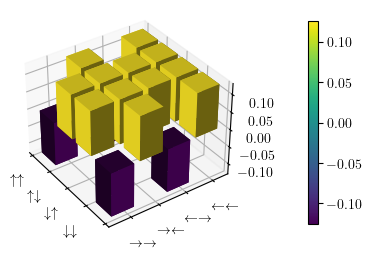
\includegraphics[width=0.6\textwidth]{imgs/wigner-desargues-2-2-s2.png}
      \caption{Función de Wigner del estado
      $\frac{1}{\sqrt{2}} \left(
        \ket{\uparrow\downarrow} -
      \ket{\downarrow\uparrow}\right)$.}
      \label{fig:wigner-desargues-2-2-s2}
    \end{figure}
  \end{frame}

  \section{Construcción no estándar}

  \begin{frame}
    \frametitle{Construcción no estándar}

    La asignación de un conjunto maximal de MUBs a las
    rectas del espacio de fase discreto es lo que distingue
    la construcción de Wootters de otras definiciones de
    funciones de Wigner discretas.

    \vspace{15pt}

    \pause

    Pero el conjunto de rayos \textbf{no} es la única manera
    de hacer una ``partición'' del DPS. Existen muchos
    conjuntos de \textit{curvas} que también brindan
    conjuntos maximales de operadores de desplazamiento
    conmutativos.

    \vspace{15pt}

    \pause

    Kantor et al, vinculan la construcción de MUBs con
    \textit{planos afínes} y \textit{coberturas
    simplécticas}.
  \end{frame}

  

  \subsection{Coberturas simplécticas}

  \begin{frame}
    \frametitle{Coberturas simplécticas y MUBs}

    \begin{definition}[Cobertura simpléctica]
      Una cobertura simpléctica $\Sigma$ de un espacio
      simpléctico $W = \F \oplus \F$ es una familia $\Sigma$ 
      de $d+1$ subespacios de $W$, de dimensión $k$ 
      totalmente isotrópicos, tales que su intersección
      uno-a-uno es el espacio trivial.
    \end{definition}

    \pause

    \begin{theorem}[Kantor, 2.3]
      Toda cobertura simpléctica $\Sigma$ determina un
      conjunto completo de $d+1$ MUBs en $\C^{d}$. Además,
      si $\Sigma'$ es otra cobertura simpléctica, entonces
      $\Sigma$ y $\Sigma'$ son equivalentes bajo una
      transformación lineal de $\F \oplus \F$ que preserva
      la forma bilineal alternante, si y solo si las MUBs
      respecto a $\Sigma$ y $\Sigma'$ son equivalentes bajo
      una transformación unitaria de $\C^{d}$.
    \end{theorem}
  \end{frame}

  \begin{frame}
    \frametitle{¿Cómo generar coberturas simplécticas?}

    La mayoría de las coberturas simplécticas pueden ser
    generadas a partir de presemicampos y semicampos. La
    cobertura $\Sigma$ generada por la operación del
    presemicampo $\circ$ consiste de los subespacios 
    \begin{equation}
      \{(0,v) : v \in \F\},
      \quad
      \{(u,u\circ m) : u \in \F\},
      \quad \text{para todo } m \in \F.
    \end{equation}

    \vspace{5pt}

    \pause

    \begin{example}
      Las rectas de Wootters corresponden a los subespacios
      unidimensionales del espacio de fase. En éste caso la
      operación $\circ$ es la operación del campo y el plano
      afín generado por la cobertura es
      \begin{equation}
        x = 0
        \quad
        \text{ y }
        \quad
        y = mx
        \quad \text{para todo } m \in \F,
      \end{equation}
      también conocido como el plano de \textit{Desargues}.
    \end{example}
  \end{frame}

  \begin{frame}
    \frametitle{Ejemplo}

    \begin{figure}[h]
      \centering
      \scalebox{0.45}{
        %% Creator: Matplotlib, PGF backend
%%
%% To include the figure in your LaTeX document, write
%%   \input{<filename>.pgf}
%%
%% Make sure the required packages are loaded in your preamble
%%   \usepackage{pgf}
%%
%% Also ensure that all the required font packages are loaded; for instance,
%% the lmodern package is sometimes necessary when using math font.
%%   \usepackage{lmodern}
%%
%% Figures using additional raster images can only be included by \input if
%% they are in the same directory as the main LaTeX file. For loading figures
%% from other directories you can use the `import` package
%%   \usepackage{import}
%%
%% and then include the figures with
%%   \import{<path to file>}{<filename>.pgf}
%%
%% Matplotlib used the following preamble
%%   
%%   \makeatletter\@ifpackageloaded{underscore}{}{\usepackage[strings]{underscore}}\makeatother
%%
\begingroup%
\makeatletter%
\begin{pgfpicture}%
\pgfpathrectangle{\pgfpointorigin}{\pgfqpoint{4.500000in}{4.500000in}}%
\pgfusepath{use as bounding box, clip}%
\begin{pgfscope}%
\pgfsetbuttcap%
\pgfsetmiterjoin%
\definecolor{currentfill}{rgb}{1.000000,1.000000,1.000000}%
\pgfsetfillcolor{currentfill}%
\pgfsetlinewidth{0.000000pt}%
\definecolor{currentstroke}{rgb}{1.000000,1.000000,1.000000}%
\pgfsetstrokecolor{currentstroke}%
\pgfsetdash{}{0pt}%
\pgfpathmoveto{\pgfqpoint{0.000000in}{0.000000in}}%
\pgfpathlineto{\pgfqpoint{4.500000in}{0.000000in}}%
\pgfpathlineto{\pgfqpoint{4.500000in}{4.500000in}}%
\pgfpathlineto{\pgfqpoint{0.000000in}{4.500000in}}%
\pgfpathlineto{\pgfqpoint{0.000000in}{0.000000in}}%
\pgfpathclose%
\pgfusepath{fill}%
\end{pgfscope}%
\begin{pgfscope}%
\pgfsetbuttcap%
\pgfsetmiterjoin%
\definecolor{currentfill}{rgb}{1.000000,1.000000,1.000000}%
\pgfsetfillcolor{currentfill}%
\pgfsetlinewidth{0.000000pt}%
\definecolor{currentstroke}{rgb}{0.000000,0.000000,0.000000}%
\pgfsetstrokecolor{currentstroke}%
\pgfsetstrokeopacity{0.000000}%
\pgfsetdash{}{0pt}%
\pgfpathmoveto{\pgfqpoint{0.562500in}{0.495000in}}%
\pgfpathlineto{\pgfqpoint{4.050000in}{0.495000in}}%
\pgfpathlineto{\pgfqpoint{4.050000in}{3.960000in}}%
\pgfpathlineto{\pgfqpoint{0.562500in}{3.960000in}}%
\pgfpathlineto{\pgfqpoint{0.562500in}{0.495000in}}%
\pgfpathclose%
\pgfusepath{fill}%
\end{pgfscope}%
\begin{pgfscope}%
\pgfsetbuttcap%
\pgfsetroundjoin%
\definecolor{currentfill}{rgb}{0.000000,0.000000,0.000000}%
\pgfsetfillcolor{currentfill}%
\pgfsetlinewidth{0.803000pt}%
\definecolor{currentstroke}{rgb}{0.000000,0.000000,0.000000}%
\pgfsetstrokecolor{currentstroke}%
\pgfsetdash{}{0pt}%
\pgfsys@defobject{currentmarker}{\pgfqpoint{0.000000in}{-0.048611in}}{\pgfqpoint{0.000000in}{0.000000in}}{%
\pgfpathmoveto{\pgfqpoint{0.000000in}{0.000000in}}%
\pgfpathlineto{\pgfqpoint{0.000000in}{-0.048611in}}%
\pgfusepath{stroke,fill}%
}%
\begin{pgfscope}%
\pgfsys@transformshift{0.721023in}{0.495000in}%
\pgfsys@useobject{currentmarker}{}%
\end{pgfscope}%
\end{pgfscope}%
\begin{pgfscope}%
\definecolor{textcolor}{rgb}{0.000000,0.000000,0.000000}%
\pgfsetstrokecolor{textcolor}%
\pgfsetfillcolor{textcolor}%
\pgftext[x=0.721023in,y=0.397778in,,top]{\color{textcolor}\rmfamily\fontsize{10.000000}{12.000000}\selectfont \(\displaystyle {0}\)}%
\end{pgfscope}%
\begin{pgfscope}%
\pgfsetbuttcap%
\pgfsetroundjoin%
\definecolor{currentfill}{rgb}{0.000000,0.000000,0.000000}%
\pgfsetfillcolor{currentfill}%
\pgfsetlinewidth{0.803000pt}%
\definecolor{currentstroke}{rgb}{0.000000,0.000000,0.000000}%
\pgfsetstrokecolor{currentstroke}%
\pgfsetdash{}{0pt}%
\pgfsys@defobject{currentmarker}{\pgfqpoint{0.000000in}{-0.048611in}}{\pgfqpoint{0.000000in}{0.000000in}}{%
\pgfpathmoveto{\pgfqpoint{0.000000in}{0.000000in}}%
\pgfpathlineto{\pgfqpoint{0.000000in}{-0.048611in}}%
\pgfusepath{stroke,fill}%
}%
\begin{pgfscope}%
\pgfsys@transformshift{1.330726in}{0.495000in}%
\pgfsys@useobject{currentmarker}{}%
\end{pgfscope}%
\end{pgfscope}%
\begin{pgfscope}%
\definecolor{textcolor}{rgb}{0.000000,0.000000,0.000000}%
\pgfsetstrokecolor{textcolor}%
\pgfsetfillcolor{textcolor}%
\pgftext[x=1.330726in,y=0.397778in,,top]{\color{textcolor}\rmfamily\fontsize{10.000000}{12.000000}\selectfont \(\displaystyle {5}\)}%
\end{pgfscope}%
\begin{pgfscope}%
\pgfsetbuttcap%
\pgfsetroundjoin%
\definecolor{currentfill}{rgb}{0.000000,0.000000,0.000000}%
\pgfsetfillcolor{currentfill}%
\pgfsetlinewidth{0.803000pt}%
\definecolor{currentstroke}{rgb}{0.000000,0.000000,0.000000}%
\pgfsetstrokecolor{currentstroke}%
\pgfsetdash{}{0pt}%
\pgfsys@defobject{currentmarker}{\pgfqpoint{0.000000in}{-0.048611in}}{\pgfqpoint{0.000000in}{0.000000in}}{%
\pgfpathmoveto{\pgfqpoint{0.000000in}{0.000000in}}%
\pgfpathlineto{\pgfqpoint{0.000000in}{-0.048611in}}%
\pgfusepath{stroke,fill}%
}%
\begin{pgfscope}%
\pgfsys@transformshift{1.940428in}{0.495000in}%
\pgfsys@useobject{currentmarker}{}%
\end{pgfscope}%
\end{pgfscope}%
\begin{pgfscope}%
\definecolor{textcolor}{rgb}{0.000000,0.000000,0.000000}%
\pgfsetstrokecolor{textcolor}%
\pgfsetfillcolor{textcolor}%
\pgftext[x=1.940428in,y=0.397778in,,top]{\color{textcolor}\rmfamily\fontsize{10.000000}{12.000000}\selectfont \(\displaystyle {10}\)}%
\end{pgfscope}%
\begin{pgfscope}%
\pgfsetbuttcap%
\pgfsetroundjoin%
\definecolor{currentfill}{rgb}{0.000000,0.000000,0.000000}%
\pgfsetfillcolor{currentfill}%
\pgfsetlinewidth{0.803000pt}%
\definecolor{currentstroke}{rgb}{0.000000,0.000000,0.000000}%
\pgfsetstrokecolor{currentstroke}%
\pgfsetdash{}{0pt}%
\pgfsys@defobject{currentmarker}{\pgfqpoint{0.000000in}{-0.048611in}}{\pgfqpoint{0.000000in}{0.000000in}}{%
\pgfpathmoveto{\pgfqpoint{0.000000in}{0.000000in}}%
\pgfpathlineto{\pgfqpoint{0.000000in}{-0.048611in}}%
\pgfusepath{stroke,fill}%
}%
\begin{pgfscope}%
\pgfsys@transformshift{2.550131in}{0.495000in}%
\pgfsys@useobject{currentmarker}{}%
\end{pgfscope}%
\end{pgfscope}%
\begin{pgfscope}%
\definecolor{textcolor}{rgb}{0.000000,0.000000,0.000000}%
\pgfsetstrokecolor{textcolor}%
\pgfsetfillcolor{textcolor}%
\pgftext[x=2.550131in,y=0.397778in,,top]{\color{textcolor}\rmfamily\fontsize{10.000000}{12.000000}\selectfont \(\displaystyle {15}\)}%
\end{pgfscope}%
\begin{pgfscope}%
\pgfsetbuttcap%
\pgfsetroundjoin%
\definecolor{currentfill}{rgb}{0.000000,0.000000,0.000000}%
\pgfsetfillcolor{currentfill}%
\pgfsetlinewidth{0.803000pt}%
\definecolor{currentstroke}{rgb}{0.000000,0.000000,0.000000}%
\pgfsetstrokecolor{currentstroke}%
\pgfsetdash{}{0pt}%
\pgfsys@defobject{currentmarker}{\pgfqpoint{0.000000in}{-0.048611in}}{\pgfqpoint{0.000000in}{0.000000in}}{%
\pgfpathmoveto{\pgfqpoint{0.000000in}{0.000000in}}%
\pgfpathlineto{\pgfqpoint{0.000000in}{-0.048611in}}%
\pgfusepath{stroke,fill}%
}%
\begin{pgfscope}%
\pgfsys@transformshift{3.159834in}{0.495000in}%
\pgfsys@useobject{currentmarker}{}%
\end{pgfscope}%
\end{pgfscope}%
\begin{pgfscope}%
\definecolor{textcolor}{rgb}{0.000000,0.000000,0.000000}%
\pgfsetstrokecolor{textcolor}%
\pgfsetfillcolor{textcolor}%
\pgftext[x=3.159834in,y=0.397778in,,top]{\color{textcolor}\rmfamily\fontsize{10.000000}{12.000000}\selectfont \(\displaystyle {20}\)}%
\end{pgfscope}%
\begin{pgfscope}%
\pgfsetbuttcap%
\pgfsetroundjoin%
\definecolor{currentfill}{rgb}{0.000000,0.000000,0.000000}%
\pgfsetfillcolor{currentfill}%
\pgfsetlinewidth{0.803000pt}%
\definecolor{currentstroke}{rgb}{0.000000,0.000000,0.000000}%
\pgfsetstrokecolor{currentstroke}%
\pgfsetdash{}{0pt}%
\pgfsys@defobject{currentmarker}{\pgfqpoint{0.000000in}{-0.048611in}}{\pgfqpoint{0.000000in}{0.000000in}}{%
\pgfpathmoveto{\pgfqpoint{0.000000in}{0.000000in}}%
\pgfpathlineto{\pgfqpoint{0.000000in}{-0.048611in}}%
\pgfusepath{stroke,fill}%
}%
\begin{pgfscope}%
\pgfsys@transformshift{3.769537in}{0.495000in}%
\pgfsys@useobject{currentmarker}{}%
\end{pgfscope}%
\end{pgfscope}%
\begin{pgfscope}%
\definecolor{textcolor}{rgb}{0.000000,0.000000,0.000000}%
\pgfsetstrokecolor{textcolor}%
\pgfsetfillcolor{textcolor}%
\pgftext[x=3.769537in,y=0.397778in,,top]{\color{textcolor}\rmfamily\fontsize{10.000000}{12.000000}\selectfont \(\displaystyle {25}\)}%
\end{pgfscope}%
\begin{pgfscope}%
\pgfsetbuttcap%
\pgfsetroundjoin%
\definecolor{currentfill}{rgb}{0.000000,0.000000,0.000000}%
\pgfsetfillcolor{currentfill}%
\pgfsetlinewidth{0.803000pt}%
\definecolor{currentstroke}{rgb}{0.000000,0.000000,0.000000}%
\pgfsetstrokecolor{currentstroke}%
\pgfsetdash{}{0pt}%
\pgfsys@defobject{currentmarker}{\pgfqpoint{-0.048611in}{0.000000in}}{\pgfqpoint{-0.000000in}{0.000000in}}{%
\pgfpathmoveto{\pgfqpoint{-0.000000in}{0.000000in}}%
\pgfpathlineto{\pgfqpoint{-0.048611in}{0.000000in}}%
\pgfusepath{stroke,fill}%
}%
\begin{pgfscope}%
\pgfsys@transformshift{0.562500in}{0.652500in}%
\pgfsys@useobject{currentmarker}{}%
\end{pgfscope}%
\end{pgfscope}%
\begin{pgfscope}%
\definecolor{textcolor}{rgb}{0.000000,0.000000,0.000000}%
\pgfsetstrokecolor{textcolor}%
\pgfsetfillcolor{textcolor}%
\pgftext[x=0.395833in, y=0.604275in, left, base]{\color{textcolor}\rmfamily\fontsize{10.000000}{12.000000}\selectfont \(\displaystyle {0}\)}%
\end{pgfscope}%
\begin{pgfscope}%
\pgfsetbuttcap%
\pgfsetroundjoin%
\definecolor{currentfill}{rgb}{0.000000,0.000000,0.000000}%
\pgfsetfillcolor{currentfill}%
\pgfsetlinewidth{0.803000pt}%
\definecolor{currentstroke}{rgb}{0.000000,0.000000,0.000000}%
\pgfsetstrokecolor{currentstroke}%
\pgfsetdash{}{0pt}%
\pgfsys@defobject{currentmarker}{\pgfqpoint{-0.048611in}{0.000000in}}{\pgfqpoint{-0.000000in}{0.000000in}}{%
\pgfpathmoveto{\pgfqpoint{-0.000000in}{0.000000in}}%
\pgfpathlineto{\pgfqpoint{-0.048611in}{0.000000in}}%
\pgfusepath{stroke,fill}%
}%
\begin{pgfscope}%
\pgfsys@transformshift{0.562500in}{1.258269in}%
\pgfsys@useobject{currentmarker}{}%
\end{pgfscope}%
\end{pgfscope}%
\begin{pgfscope}%
\definecolor{textcolor}{rgb}{0.000000,0.000000,0.000000}%
\pgfsetstrokecolor{textcolor}%
\pgfsetfillcolor{textcolor}%
\pgftext[x=0.395833in, y=1.210044in, left, base]{\color{textcolor}\rmfamily\fontsize{10.000000}{12.000000}\selectfont \(\displaystyle {5}\)}%
\end{pgfscope}%
\begin{pgfscope}%
\pgfsetbuttcap%
\pgfsetroundjoin%
\definecolor{currentfill}{rgb}{0.000000,0.000000,0.000000}%
\pgfsetfillcolor{currentfill}%
\pgfsetlinewidth{0.803000pt}%
\definecolor{currentstroke}{rgb}{0.000000,0.000000,0.000000}%
\pgfsetstrokecolor{currentstroke}%
\pgfsetdash{}{0pt}%
\pgfsys@defobject{currentmarker}{\pgfqpoint{-0.048611in}{0.000000in}}{\pgfqpoint{-0.000000in}{0.000000in}}{%
\pgfpathmoveto{\pgfqpoint{-0.000000in}{0.000000in}}%
\pgfpathlineto{\pgfqpoint{-0.048611in}{0.000000in}}%
\pgfusepath{stroke,fill}%
}%
\begin{pgfscope}%
\pgfsys@transformshift{0.562500in}{1.864038in}%
\pgfsys@useobject{currentmarker}{}%
\end{pgfscope}%
\end{pgfscope}%
\begin{pgfscope}%
\definecolor{textcolor}{rgb}{0.000000,0.000000,0.000000}%
\pgfsetstrokecolor{textcolor}%
\pgfsetfillcolor{textcolor}%
\pgftext[x=0.326388in, y=1.815813in, left, base]{\color{textcolor}\rmfamily\fontsize{10.000000}{12.000000}\selectfont \(\displaystyle {10}\)}%
\end{pgfscope}%
\begin{pgfscope}%
\pgfsetbuttcap%
\pgfsetroundjoin%
\definecolor{currentfill}{rgb}{0.000000,0.000000,0.000000}%
\pgfsetfillcolor{currentfill}%
\pgfsetlinewidth{0.803000pt}%
\definecolor{currentstroke}{rgb}{0.000000,0.000000,0.000000}%
\pgfsetstrokecolor{currentstroke}%
\pgfsetdash{}{0pt}%
\pgfsys@defobject{currentmarker}{\pgfqpoint{-0.048611in}{0.000000in}}{\pgfqpoint{-0.000000in}{0.000000in}}{%
\pgfpathmoveto{\pgfqpoint{-0.000000in}{0.000000in}}%
\pgfpathlineto{\pgfqpoint{-0.048611in}{0.000000in}}%
\pgfusepath{stroke,fill}%
}%
\begin{pgfscope}%
\pgfsys@transformshift{0.562500in}{2.469808in}%
\pgfsys@useobject{currentmarker}{}%
\end{pgfscope}%
\end{pgfscope}%
\begin{pgfscope}%
\definecolor{textcolor}{rgb}{0.000000,0.000000,0.000000}%
\pgfsetstrokecolor{textcolor}%
\pgfsetfillcolor{textcolor}%
\pgftext[x=0.326388in, y=2.421582in, left, base]{\color{textcolor}\rmfamily\fontsize{10.000000}{12.000000}\selectfont \(\displaystyle {15}\)}%
\end{pgfscope}%
\begin{pgfscope}%
\pgfsetbuttcap%
\pgfsetroundjoin%
\definecolor{currentfill}{rgb}{0.000000,0.000000,0.000000}%
\pgfsetfillcolor{currentfill}%
\pgfsetlinewidth{0.803000pt}%
\definecolor{currentstroke}{rgb}{0.000000,0.000000,0.000000}%
\pgfsetstrokecolor{currentstroke}%
\pgfsetdash{}{0pt}%
\pgfsys@defobject{currentmarker}{\pgfqpoint{-0.048611in}{0.000000in}}{\pgfqpoint{-0.000000in}{0.000000in}}{%
\pgfpathmoveto{\pgfqpoint{-0.000000in}{0.000000in}}%
\pgfpathlineto{\pgfqpoint{-0.048611in}{0.000000in}}%
\pgfusepath{stroke,fill}%
}%
\begin{pgfscope}%
\pgfsys@transformshift{0.562500in}{3.075577in}%
\pgfsys@useobject{currentmarker}{}%
\end{pgfscope}%
\end{pgfscope}%
\begin{pgfscope}%
\definecolor{textcolor}{rgb}{0.000000,0.000000,0.000000}%
\pgfsetstrokecolor{textcolor}%
\pgfsetfillcolor{textcolor}%
\pgftext[x=0.326388in, y=3.027352in, left, base]{\color{textcolor}\rmfamily\fontsize{10.000000}{12.000000}\selectfont \(\displaystyle {20}\)}%
\end{pgfscope}%
\begin{pgfscope}%
\pgfsetbuttcap%
\pgfsetroundjoin%
\definecolor{currentfill}{rgb}{0.000000,0.000000,0.000000}%
\pgfsetfillcolor{currentfill}%
\pgfsetlinewidth{0.803000pt}%
\definecolor{currentstroke}{rgb}{0.000000,0.000000,0.000000}%
\pgfsetstrokecolor{currentstroke}%
\pgfsetdash{}{0pt}%
\pgfsys@defobject{currentmarker}{\pgfqpoint{-0.048611in}{0.000000in}}{\pgfqpoint{-0.000000in}{0.000000in}}{%
\pgfpathmoveto{\pgfqpoint{-0.000000in}{0.000000in}}%
\pgfpathlineto{\pgfqpoint{-0.048611in}{0.000000in}}%
\pgfusepath{stroke,fill}%
}%
\begin{pgfscope}%
\pgfsys@transformshift{0.562500in}{3.681346in}%
\pgfsys@useobject{currentmarker}{}%
\end{pgfscope}%
\end{pgfscope}%
\begin{pgfscope}%
\definecolor{textcolor}{rgb}{0.000000,0.000000,0.000000}%
\pgfsetstrokecolor{textcolor}%
\pgfsetfillcolor{textcolor}%
\pgftext[x=0.326388in, y=3.633121in, left, base]{\color{textcolor}\rmfamily\fontsize{10.000000}{12.000000}\selectfont \(\displaystyle {25}\)}%
\end{pgfscope}%
\begin{pgfscope}%
\pgfpathrectangle{\pgfqpoint{0.562500in}{0.495000in}}{\pgfqpoint{3.487500in}{3.465000in}}%
\pgfusepath{clip}%
\pgfsetrectcap%
\pgfsetroundjoin%
\pgfsetlinewidth{0.000000pt}%
\definecolor{currentstroke}{rgb}{0.121569,0.466667,0.705882}%
\pgfsetstrokecolor{currentstroke}%
\pgfsetstrokeopacity{0.900000}%
\pgfsetdash{}{0pt}%
\pgfpathmoveto{\pgfqpoint{0.721023in}{0.652500in}}%
\pgfpathlineto{\pgfqpoint{0.721023in}{0.773654in}}%
\pgfpathlineto{\pgfqpoint{0.721023in}{0.894808in}}%
\pgfpathlineto{\pgfqpoint{0.721023in}{1.015962in}}%
\pgfpathlineto{\pgfqpoint{0.721023in}{1.137115in}}%
\pgfpathlineto{\pgfqpoint{0.721023in}{1.258269in}}%
\pgfpathlineto{\pgfqpoint{0.721023in}{1.379423in}}%
\pgfpathlineto{\pgfqpoint{0.721023in}{1.500577in}}%
\pgfpathlineto{\pgfqpoint{0.721023in}{1.621731in}}%
\pgfpathlineto{\pgfqpoint{0.721023in}{1.742885in}}%
\pgfpathlineto{\pgfqpoint{0.721023in}{1.864038in}}%
\pgfpathlineto{\pgfqpoint{0.721023in}{1.985192in}}%
\pgfpathlineto{\pgfqpoint{0.721023in}{2.106346in}}%
\pgfpathlineto{\pgfqpoint{0.721023in}{2.227500in}}%
\pgfpathlineto{\pgfqpoint{0.721023in}{2.348654in}}%
\pgfpathlineto{\pgfqpoint{0.721023in}{2.469808in}}%
\pgfpathlineto{\pgfqpoint{0.721023in}{2.590962in}}%
\pgfpathlineto{\pgfqpoint{0.721023in}{2.712115in}}%
\pgfpathlineto{\pgfqpoint{0.721023in}{2.833269in}}%
\pgfpathlineto{\pgfqpoint{0.721023in}{2.954423in}}%
\pgfpathlineto{\pgfqpoint{0.721023in}{3.075577in}}%
\pgfpathlineto{\pgfqpoint{0.721023in}{3.196731in}}%
\pgfpathlineto{\pgfqpoint{0.721023in}{3.317885in}}%
\pgfpathlineto{\pgfqpoint{0.721023in}{3.439038in}}%
\pgfpathlineto{\pgfqpoint{0.721023in}{3.560192in}}%
\pgfpathlineto{\pgfqpoint{0.721023in}{3.681346in}}%
\pgfpathlineto{\pgfqpoint{0.721023in}{3.802500in}}%
\pgfusepath{}%
\end{pgfscope}%
\begin{pgfscope}%
\pgfpathrectangle{\pgfqpoint{0.562500in}{0.495000in}}{\pgfqpoint{3.487500in}{3.465000in}}%
\pgfusepath{clip}%
\pgfsetbuttcap%
\pgfsetroundjoin%
\definecolor{currentfill}{rgb}{0.121569,0.466667,0.705882}%
\pgfsetfillcolor{currentfill}%
\pgfsetfillopacity{0.900000}%
\pgfsetlinewidth{1.003750pt}%
\definecolor{currentstroke}{rgb}{0.121569,0.466667,0.705882}%
\pgfsetstrokecolor{currentstroke}%
\pgfsetstrokeopacity{0.900000}%
\pgfsetdash{}{0pt}%
\pgfsys@defobject{currentmarker}{\pgfqpoint{-0.027778in}{-0.027778in}}{\pgfqpoint{0.027778in}{0.027778in}}{%
\pgfpathmoveto{\pgfqpoint{0.000000in}{-0.027778in}}%
\pgfpathcurveto{\pgfqpoint{0.007367in}{-0.027778in}}{\pgfqpoint{0.014433in}{-0.024851in}}{\pgfqpoint{0.019642in}{-0.019642in}}%
\pgfpathcurveto{\pgfqpoint{0.024851in}{-0.014433in}}{\pgfqpoint{0.027778in}{-0.007367in}}{\pgfqpoint{0.027778in}{0.000000in}}%
\pgfpathcurveto{\pgfqpoint{0.027778in}{0.007367in}}{\pgfqpoint{0.024851in}{0.014433in}}{\pgfqpoint{0.019642in}{0.019642in}}%
\pgfpathcurveto{\pgfqpoint{0.014433in}{0.024851in}}{\pgfqpoint{0.007367in}{0.027778in}}{\pgfqpoint{0.000000in}{0.027778in}}%
\pgfpathcurveto{\pgfqpoint{-0.007367in}{0.027778in}}{\pgfqpoint{-0.014433in}{0.024851in}}{\pgfqpoint{-0.019642in}{0.019642in}}%
\pgfpathcurveto{\pgfqpoint{-0.024851in}{0.014433in}}{\pgfqpoint{-0.027778in}{0.007367in}}{\pgfqpoint{-0.027778in}{0.000000in}}%
\pgfpathcurveto{\pgfqpoint{-0.027778in}{-0.007367in}}{\pgfqpoint{-0.024851in}{-0.014433in}}{\pgfqpoint{-0.019642in}{-0.019642in}}%
\pgfpathcurveto{\pgfqpoint{-0.014433in}{-0.024851in}}{\pgfqpoint{-0.007367in}{-0.027778in}}{\pgfqpoint{0.000000in}{-0.027778in}}%
\pgfpathlineto{\pgfqpoint{0.000000in}{-0.027778in}}%
\pgfpathclose%
\pgfusepath{stroke,fill}%
}%
\begin{pgfscope}%
\pgfsys@transformshift{0.721023in}{0.652500in}%
\pgfsys@useobject{currentmarker}{}%
\end{pgfscope}%
\begin{pgfscope}%
\pgfsys@transformshift{0.721023in}{0.773654in}%
\pgfsys@useobject{currentmarker}{}%
\end{pgfscope}%
\begin{pgfscope}%
\pgfsys@transformshift{0.721023in}{0.894808in}%
\pgfsys@useobject{currentmarker}{}%
\end{pgfscope}%
\begin{pgfscope}%
\pgfsys@transformshift{0.721023in}{1.015962in}%
\pgfsys@useobject{currentmarker}{}%
\end{pgfscope}%
\begin{pgfscope}%
\pgfsys@transformshift{0.721023in}{1.137115in}%
\pgfsys@useobject{currentmarker}{}%
\end{pgfscope}%
\begin{pgfscope}%
\pgfsys@transformshift{0.721023in}{1.258269in}%
\pgfsys@useobject{currentmarker}{}%
\end{pgfscope}%
\begin{pgfscope}%
\pgfsys@transformshift{0.721023in}{1.379423in}%
\pgfsys@useobject{currentmarker}{}%
\end{pgfscope}%
\begin{pgfscope}%
\pgfsys@transformshift{0.721023in}{1.500577in}%
\pgfsys@useobject{currentmarker}{}%
\end{pgfscope}%
\begin{pgfscope}%
\pgfsys@transformshift{0.721023in}{1.621731in}%
\pgfsys@useobject{currentmarker}{}%
\end{pgfscope}%
\begin{pgfscope}%
\pgfsys@transformshift{0.721023in}{1.742885in}%
\pgfsys@useobject{currentmarker}{}%
\end{pgfscope}%
\begin{pgfscope}%
\pgfsys@transformshift{0.721023in}{1.864038in}%
\pgfsys@useobject{currentmarker}{}%
\end{pgfscope}%
\begin{pgfscope}%
\pgfsys@transformshift{0.721023in}{1.985192in}%
\pgfsys@useobject{currentmarker}{}%
\end{pgfscope}%
\begin{pgfscope}%
\pgfsys@transformshift{0.721023in}{2.106346in}%
\pgfsys@useobject{currentmarker}{}%
\end{pgfscope}%
\begin{pgfscope}%
\pgfsys@transformshift{0.721023in}{2.227500in}%
\pgfsys@useobject{currentmarker}{}%
\end{pgfscope}%
\begin{pgfscope}%
\pgfsys@transformshift{0.721023in}{2.348654in}%
\pgfsys@useobject{currentmarker}{}%
\end{pgfscope}%
\begin{pgfscope}%
\pgfsys@transformshift{0.721023in}{2.469808in}%
\pgfsys@useobject{currentmarker}{}%
\end{pgfscope}%
\begin{pgfscope}%
\pgfsys@transformshift{0.721023in}{2.590962in}%
\pgfsys@useobject{currentmarker}{}%
\end{pgfscope}%
\begin{pgfscope}%
\pgfsys@transformshift{0.721023in}{2.712115in}%
\pgfsys@useobject{currentmarker}{}%
\end{pgfscope}%
\begin{pgfscope}%
\pgfsys@transformshift{0.721023in}{2.833269in}%
\pgfsys@useobject{currentmarker}{}%
\end{pgfscope}%
\begin{pgfscope}%
\pgfsys@transformshift{0.721023in}{2.954423in}%
\pgfsys@useobject{currentmarker}{}%
\end{pgfscope}%
\begin{pgfscope}%
\pgfsys@transformshift{0.721023in}{3.075577in}%
\pgfsys@useobject{currentmarker}{}%
\end{pgfscope}%
\begin{pgfscope}%
\pgfsys@transformshift{0.721023in}{3.196731in}%
\pgfsys@useobject{currentmarker}{}%
\end{pgfscope}%
\begin{pgfscope}%
\pgfsys@transformshift{0.721023in}{3.317885in}%
\pgfsys@useobject{currentmarker}{}%
\end{pgfscope}%
\begin{pgfscope}%
\pgfsys@transformshift{0.721023in}{3.439038in}%
\pgfsys@useobject{currentmarker}{}%
\end{pgfscope}%
\begin{pgfscope}%
\pgfsys@transformshift{0.721023in}{3.560192in}%
\pgfsys@useobject{currentmarker}{}%
\end{pgfscope}%
\begin{pgfscope}%
\pgfsys@transformshift{0.721023in}{3.681346in}%
\pgfsys@useobject{currentmarker}{}%
\end{pgfscope}%
\begin{pgfscope}%
\pgfsys@transformshift{0.721023in}{3.802500in}%
\pgfsys@useobject{currentmarker}{}%
\end{pgfscope}%
\end{pgfscope}%
\begin{pgfscope}%
\pgfpathrectangle{\pgfqpoint{0.562500in}{0.495000in}}{\pgfqpoint{3.487500in}{3.465000in}}%
\pgfusepath{clip}%
\pgfsetrectcap%
\pgfsetroundjoin%
\pgfsetlinewidth{0.000000pt}%
\definecolor{currentstroke}{rgb}{1.000000,0.498039,0.054902}%
\pgfsetstrokecolor{currentstroke}%
\pgfsetstrokeopacity{0.900000}%
\pgfsetdash{}{0pt}%
\pgfpathmoveto{\pgfqpoint{0.721023in}{0.652500in}}%
\pgfpathlineto{\pgfqpoint{0.842963in}{0.652500in}}%
\pgfpathlineto{\pgfqpoint{0.964904in}{0.652500in}}%
\pgfpathlineto{\pgfqpoint{1.086844in}{0.652500in}}%
\pgfpathlineto{\pgfqpoint{1.208785in}{0.652500in}}%
\pgfpathlineto{\pgfqpoint{1.330726in}{0.652500in}}%
\pgfpathlineto{\pgfqpoint{1.452666in}{0.652500in}}%
\pgfpathlineto{\pgfqpoint{1.574607in}{0.652500in}}%
\pgfpathlineto{\pgfqpoint{1.696547in}{0.652500in}}%
\pgfpathlineto{\pgfqpoint{1.818488in}{0.652500in}}%
\pgfpathlineto{\pgfqpoint{1.940428in}{0.652500in}}%
\pgfpathlineto{\pgfqpoint{2.062369in}{0.652500in}}%
\pgfpathlineto{\pgfqpoint{2.184309in}{0.652500in}}%
\pgfpathlineto{\pgfqpoint{2.306250in}{0.652500in}}%
\pgfpathlineto{\pgfqpoint{2.428191in}{0.652500in}}%
\pgfpathlineto{\pgfqpoint{2.550131in}{0.652500in}}%
\pgfpathlineto{\pgfqpoint{2.672072in}{0.652500in}}%
\pgfpathlineto{\pgfqpoint{2.794012in}{0.652500in}}%
\pgfpathlineto{\pgfqpoint{2.915953in}{0.652500in}}%
\pgfpathlineto{\pgfqpoint{3.037893in}{0.652500in}}%
\pgfpathlineto{\pgfqpoint{3.159834in}{0.652500in}}%
\pgfpathlineto{\pgfqpoint{3.281774in}{0.652500in}}%
\pgfpathlineto{\pgfqpoint{3.403715in}{0.652500in}}%
\pgfpathlineto{\pgfqpoint{3.525656in}{0.652500in}}%
\pgfpathlineto{\pgfqpoint{3.647596in}{0.652500in}}%
\pgfpathlineto{\pgfqpoint{3.769537in}{0.652500in}}%
\pgfpathlineto{\pgfqpoint{3.891477in}{0.652500in}}%
\pgfusepath{}%
\end{pgfscope}%
\begin{pgfscope}%
\pgfpathrectangle{\pgfqpoint{0.562500in}{0.495000in}}{\pgfqpoint{3.487500in}{3.465000in}}%
\pgfusepath{clip}%
\pgfsetbuttcap%
\pgfsetroundjoin%
\definecolor{currentfill}{rgb}{1.000000,0.498039,0.054902}%
\pgfsetfillcolor{currentfill}%
\pgfsetfillopacity{0.900000}%
\pgfsetlinewidth{1.003750pt}%
\definecolor{currentstroke}{rgb}{1.000000,0.498039,0.054902}%
\pgfsetstrokecolor{currentstroke}%
\pgfsetstrokeopacity{0.900000}%
\pgfsetdash{}{0pt}%
\pgfsys@defobject{currentmarker}{\pgfqpoint{-0.027778in}{-0.027778in}}{\pgfqpoint{0.027778in}{0.027778in}}{%
\pgfpathmoveto{\pgfqpoint{0.000000in}{-0.027778in}}%
\pgfpathcurveto{\pgfqpoint{0.007367in}{-0.027778in}}{\pgfqpoint{0.014433in}{-0.024851in}}{\pgfqpoint{0.019642in}{-0.019642in}}%
\pgfpathcurveto{\pgfqpoint{0.024851in}{-0.014433in}}{\pgfqpoint{0.027778in}{-0.007367in}}{\pgfqpoint{0.027778in}{0.000000in}}%
\pgfpathcurveto{\pgfqpoint{0.027778in}{0.007367in}}{\pgfqpoint{0.024851in}{0.014433in}}{\pgfqpoint{0.019642in}{0.019642in}}%
\pgfpathcurveto{\pgfqpoint{0.014433in}{0.024851in}}{\pgfqpoint{0.007367in}{0.027778in}}{\pgfqpoint{0.000000in}{0.027778in}}%
\pgfpathcurveto{\pgfqpoint{-0.007367in}{0.027778in}}{\pgfqpoint{-0.014433in}{0.024851in}}{\pgfqpoint{-0.019642in}{0.019642in}}%
\pgfpathcurveto{\pgfqpoint{-0.024851in}{0.014433in}}{\pgfqpoint{-0.027778in}{0.007367in}}{\pgfqpoint{-0.027778in}{0.000000in}}%
\pgfpathcurveto{\pgfqpoint{-0.027778in}{-0.007367in}}{\pgfqpoint{-0.024851in}{-0.014433in}}{\pgfqpoint{-0.019642in}{-0.019642in}}%
\pgfpathcurveto{\pgfqpoint{-0.014433in}{-0.024851in}}{\pgfqpoint{-0.007367in}{-0.027778in}}{\pgfqpoint{0.000000in}{-0.027778in}}%
\pgfpathlineto{\pgfqpoint{0.000000in}{-0.027778in}}%
\pgfpathclose%
\pgfusepath{stroke,fill}%
}%
\begin{pgfscope}%
\pgfsys@transformshift{0.721023in}{0.652500in}%
\pgfsys@useobject{currentmarker}{}%
\end{pgfscope}%
\begin{pgfscope}%
\pgfsys@transformshift{0.842963in}{0.652500in}%
\pgfsys@useobject{currentmarker}{}%
\end{pgfscope}%
\begin{pgfscope}%
\pgfsys@transformshift{0.964904in}{0.652500in}%
\pgfsys@useobject{currentmarker}{}%
\end{pgfscope}%
\begin{pgfscope}%
\pgfsys@transformshift{1.086844in}{0.652500in}%
\pgfsys@useobject{currentmarker}{}%
\end{pgfscope}%
\begin{pgfscope}%
\pgfsys@transformshift{1.208785in}{0.652500in}%
\pgfsys@useobject{currentmarker}{}%
\end{pgfscope}%
\begin{pgfscope}%
\pgfsys@transformshift{1.330726in}{0.652500in}%
\pgfsys@useobject{currentmarker}{}%
\end{pgfscope}%
\begin{pgfscope}%
\pgfsys@transformshift{1.452666in}{0.652500in}%
\pgfsys@useobject{currentmarker}{}%
\end{pgfscope}%
\begin{pgfscope}%
\pgfsys@transformshift{1.574607in}{0.652500in}%
\pgfsys@useobject{currentmarker}{}%
\end{pgfscope}%
\begin{pgfscope}%
\pgfsys@transformshift{1.696547in}{0.652500in}%
\pgfsys@useobject{currentmarker}{}%
\end{pgfscope}%
\begin{pgfscope}%
\pgfsys@transformshift{1.818488in}{0.652500in}%
\pgfsys@useobject{currentmarker}{}%
\end{pgfscope}%
\begin{pgfscope}%
\pgfsys@transformshift{1.940428in}{0.652500in}%
\pgfsys@useobject{currentmarker}{}%
\end{pgfscope}%
\begin{pgfscope}%
\pgfsys@transformshift{2.062369in}{0.652500in}%
\pgfsys@useobject{currentmarker}{}%
\end{pgfscope}%
\begin{pgfscope}%
\pgfsys@transformshift{2.184309in}{0.652500in}%
\pgfsys@useobject{currentmarker}{}%
\end{pgfscope}%
\begin{pgfscope}%
\pgfsys@transformshift{2.306250in}{0.652500in}%
\pgfsys@useobject{currentmarker}{}%
\end{pgfscope}%
\begin{pgfscope}%
\pgfsys@transformshift{2.428191in}{0.652500in}%
\pgfsys@useobject{currentmarker}{}%
\end{pgfscope}%
\begin{pgfscope}%
\pgfsys@transformshift{2.550131in}{0.652500in}%
\pgfsys@useobject{currentmarker}{}%
\end{pgfscope}%
\begin{pgfscope}%
\pgfsys@transformshift{2.672072in}{0.652500in}%
\pgfsys@useobject{currentmarker}{}%
\end{pgfscope}%
\begin{pgfscope}%
\pgfsys@transformshift{2.794012in}{0.652500in}%
\pgfsys@useobject{currentmarker}{}%
\end{pgfscope}%
\begin{pgfscope}%
\pgfsys@transformshift{2.915953in}{0.652500in}%
\pgfsys@useobject{currentmarker}{}%
\end{pgfscope}%
\begin{pgfscope}%
\pgfsys@transformshift{3.037893in}{0.652500in}%
\pgfsys@useobject{currentmarker}{}%
\end{pgfscope}%
\begin{pgfscope}%
\pgfsys@transformshift{3.159834in}{0.652500in}%
\pgfsys@useobject{currentmarker}{}%
\end{pgfscope}%
\begin{pgfscope}%
\pgfsys@transformshift{3.281774in}{0.652500in}%
\pgfsys@useobject{currentmarker}{}%
\end{pgfscope}%
\begin{pgfscope}%
\pgfsys@transformshift{3.403715in}{0.652500in}%
\pgfsys@useobject{currentmarker}{}%
\end{pgfscope}%
\begin{pgfscope}%
\pgfsys@transformshift{3.525656in}{0.652500in}%
\pgfsys@useobject{currentmarker}{}%
\end{pgfscope}%
\begin{pgfscope}%
\pgfsys@transformshift{3.647596in}{0.652500in}%
\pgfsys@useobject{currentmarker}{}%
\end{pgfscope}%
\begin{pgfscope}%
\pgfsys@transformshift{3.769537in}{0.652500in}%
\pgfsys@useobject{currentmarker}{}%
\end{pgfscope}%
\begin{pgfscope}%
\pgfsys@transformshift{3.891477in}{0.652500in}%
\pgfsys@useobject{currentmarker}{}%
\end{pgfscope}%
\end{pgfscope}%
\begin{pgfscope}%
\pgfpathrectangle{\pgfqpoint{0.562500in}{0.495000in}}{\pgfqpoint{3.487500in}{3.465000in}}%
\pgfusepath{clip}%
\pgfsetrectcap%
\pgfsetroundjoin%
\pgfsetlinewidth{0.000000pt}%
\definecolor{currentstroke}{rgb}{0.172549,0.627451,0.172549}%
\pgfsetstrokecolor{currentstroke}%
\pgfsetstrokeopacity{0.200000}%
\pgfsetdash{}{0pt}%
\pgfpathmoveto{\pgfqpoint{0.721023in}{0.652500in}}%
\pgfpathlineto{\pgfqpoint{0.842963in}{0.894808in}}%
\pgfpathlineto{\pgfqpoint{0.964904in}{1.015962in}}%
\pgfpathlineto{\pgfqpoint{1.086844in}{1.137115in}}%
\pgfpathlineto{\pgfqpoint{1.208785in}{1.258269in}}%
\pgfpathlineto{\pgfqpoint{1.330726in}{1.379423in}}%
\pgfpathlineto{\pgfqpoint{1.452666in}{1.500577in}}%
\pgfpathlineto{\pgfqpoint{1.574607in}{1.621731in}}%
\pgfpathlineto{\pgfqpoint{1.696547in}{1.742885in}}%
\pgfpathlineto{\pgfqpoint{1.818488in}{1.864038in}}%
\pgfpathlineto{\pgfqpoint{1.940428in}{1.985192in}}%
\pgfpathlineto{\pgfqpoint{2.062369in}{2.106346in}}%
\pgfpathlineto{\pgfqpoint{2.184309in}{2.227500in}}%
\pgfpathlineto{\pgfqpoint{2.306250in}{2.348654in}}%
\pgfpathlineto{\pgfqpoint{2.428191in}{2.469808in}}%
\pgfpathlineto{\pgfqpoint{2.550131in}{2.590962in}}%
\pgfpathlineto{\pgfqpoint{2.672072in}{2.712115in}}%
\pgfpathlineto{\pgfqpoint{2.794012in}{2.833269in}}%
\pgfpathlineto{\pgfqpoint{2.915953in}{2.954423in}}%
\pgfpathlineto{\pgfqpoint{3.037893in}{3.075577in}}%
\pgfpathlineto{\pgfqpoint{3.159834in}{3.196731in}}%
\pgfpathlineto{\pgfqpoint{3.281774in}{3.317885in}}%
\pgfpathlineto{\pgfqpoint{3.403715in}{3.439038in}}%
\pgfpathlineto{\pgfqpoint{3.525656in}{3.560192in}}%
\pgfpathlineto{\pgfqpoint{3.647596in}{3.681346in}}%
\pgfpathlineto{\pgfqpoint{3.769537in}{3.802500in}}%
\pgfpathlineto{\pgfqpoint{3.891477in}{0.773654in}}%
\pgfusepath{}%
\end{pgfscope}%
\begin{pgfscope}%
\pgfpathrectangle{\pgfqpoint{0.562500in}{0.495000in}}{\pgfqpoint{3.487500in}{3.465000in}}%
\pgfusepath{clip}%
\pgfsetbuttcap%
\pgfsetroundjoin%
\definecolor{currentfill}{rgb}{0.172549,0.627451,0.172549}%
\pgfsetfillcolor{currentfill}%
\pgfsetfillopacity{0.200000}%
\pgfsetlinewidth{1.003750pt}%
\definecolor{currentstroke}{rgb}{0.172549,0.627451,0.172549}%
\pgfsetstrokecolor{currentstroke}%
\pgfsetstrokeopacity{0.200000}%
\pgfsetdash{}{0pt}%
\pgfsys@defobject{currentmarker}{\pgfqpoint{-0.027778in}{-0.027778in}}{\pgfqpoint{0.027778in}{0.027778in}}{%
\pgfpathmoveto{\pgfqpoint{0.000000in}{-0.027778in}}%
\pgfpathcurveto{\pgfqpoint{0.007367in}{-0.027778in}}{\pgfqpoint{0.014433in}{-0.024851in}}{\pgfqpoint{0.019642in}{-0.019642in}}%
\pgfpathcurveto{\pgfqpoint{0.024851in}{-0.014433in}}{\pgfqpoint{0.027778in}{-0.007367in}}{\pgfqpoint{0.027778in}{0.000000in}}%
\pgfpathcurveto{\pgfqpoint{0.027778in}{0.007367in}}{\pgfqpoint{0.024851in}{0.014433in}}{\pgfqpoint{0.019642in}{0.019642in}}%
\pgfpathcurveto{\pgfqpoint{0.014433in}{0.024851in}}{\pgfqpoint{0.007367in}{0.027778in}}{\pgfqpoint{0.000000in}{0.027778in}}%
\pgfpathcurveto{\pgfqpoint{-0.007367in}{0.027778in}}{\pgfqpoint{-0.014433in}{0.024851in}}{\pgfqpoint{-0.019642in}{0.019642in}}%
\pgfpathcurveto{\pgfqpoint{-0.024851in}{0.014433in}}{\pgfqpoint{-0.027778in}{0.007367in}}{\pgfqpoint{-0.027778in}{0.000000in}}%
\pgfpathcurveto{\pgfqpoint{-0.027778in}{-0.007367in}}{\pgfqpoint{-0.024851in}{-0.014433in}}{\pgfqpoint{-0.019642in}{-0.019642in}}%
\pgfpathcurveto{\pgfqpoint{-0.014433in}{-0.024851in}}{\pgfqpoint{-0.007367in}{-0.027778in}}{\pgfqpoint{0.000000in}{-0.027778in}}%
\pgfpathlineto{\pgfqpoint{0.000000in}{-0.027778in}}%
\pgfpathclose%
\pgfusepath{stroke,fill}%
}%
\begin{pgfscope}%
\pgfsys@transformshift{0.721023in}{0.652500in}%
\pgfsys@useobject{currentmarker}{}%
\end{pgfscope}%
\begin{pgfscope}%
\pgfsys@transformshift{0.842963in}{0.894808in}%
\pgfsys@useobject{currentmarker}{}%
\end{pgfscope}%
\begin{pgfscope}%
\pgfsys@transformshift{0.964904in}{1.015962in}%
\pgfsys@useobject{currentmarker}{}%
\end{pgfscope}%
\begin{pgfscope}%
\pgfsys@transformshift{1.086844in}{1.137115in}%
\pgfsys@useobject{currentmarker}{}%
\end{pgfscope}%
\begin{pgfscope}%
\pgfsys@transformshift{1.208785in}{1.258269in}%
\pgfsys@useobject{currentmarker}{}%
\end{pgfscope}%
\begin{pgfscope}%
\pgfsys@transformshift{1.330726in}{1.379423in}%
\pgfsys@useobject{currentmarker}{}%
\end{pgfscope}%
\begin{pgfscope}%
\pgfsys@transformshift{1.452666in}{1.500577in}%
\pgfsys@useobject{currentmarker}{}%
\end{pgfscope}%
\begin{pgfscope}%
\pgfsys@transformshift{1.574607in}{1.621731in}%
\pgfsys@useobject{currentmarker}{}%
\end{pgfscope}%
\begin{pgfscope}%
\pgfsys@transformshift{1.696547in}{1.742885in}%
\pgfsys@useobject{currentmarker}{}%
\end{pgfscope}%
\begin{pgfscope}%
\pgfsys@transformshift{1.818488in}{1.864038in}%
\pgfsys@useobject{currentmarker}{}%
\end{pgfscope}%
\begin{pgfscope}%
\pgfsys@transformshift{1.940428in}{1.985192in}%
\pgfsys@useobject{currentmarker}{}%
\end{pgfscope}%
\begin{pgfscope}%
\pgfsys@transformshift{2.062369in}{2.106346in}%
\pgfsys@useobject{currentmarker}{}%
\end{pgfscope}%
\begin{pgfscope}%
\pgfsys@transformshift{2.184309in}{2.227500in}%
\pgfsys@useobject{currentmarker}{}%
\end{pgfscope}%
\begin{pgfscope}%
\pgfsys@transformshift{2.306250in}{2.348654in}%
\pgfsys@useobject{currentmarker}{}%
\end{pgfscope}%
\begin{pgfscope}%
\pgfsys@transformshift{2.428191in}{2.469808in}%
\pgfsys@useobject{currentmarker}{}%
\end{pgfscope}%
\begin{pgfscope}%
\pgfsys@transformshift{2.550131in}{2.590962in}%
\pgfsys@useobject{currentmarker}{}%
\end{pgfscope}%
\begin{pgfscope}%
\pgfsys@transformshift{2.672072in}{2.712115in}%
\pgfsys@useobject{currentmarker}{}%
\end{pgfscope}%
\begin{pgfscope}%
\pgfsys@transformshift{2.794012in}{2.833269in}%
\pgfsys@useobject{currentmarker}{}%
\end{pgfscope}%
\begin{pgfscope}%
\pgfsys@transformshift{2.915953in}{2.954423in}%
\pgfsys@useobject{currentmarker}{}%
\end{pgfscope}%
\begin{pgfscope}%
\pgfsys@transformshift{3.037893in}{3.075577in}%
\pgfsys@useobject{currentmarker}{}%
\end{pgfscope}%
\begin{pgfscope}%
\pgfsys@transformshift{3.159834in}{3.196731in}%
\pgfsys@useobject{currentmarker}{}%
\end{pgfscope}%
\begin{pgfscope}%
\pgfsys@transformshift{3.281774in}{3.317885in}%
\pgfsys@useobject{currentmarker}{}%
\end{pgfscope}%
\begin{pgfscope}%
\pgfsys@transformshift{3.403715in}{3.439038in}%
\pgfsys@useobject{currentmarker}{}%
\end{pgfscope}%
\begin{pgfscope}%
\pgfsys@transformshift{3.525656in}{3.560192in}%
\pgfsys@useobject{currentmarker}{}%
\end{pgfscope}%
\begin{pgfscope}%
\pgfsys@transformshift{3.647596in}{3.681346in}%
\pgfsys@useobject{currentmarker}{}%
\end{pgfscope}%
\begin{pgfscope}%
\pgfsys@transformshift{3.769537in}{3.802500in}%
\pgfsys@useobject{currentmarker}{}%
\end{pgfscope}%
\begin{pgfscope}%
\pgfsys@transformshift{3.891477in}{0.773654in}%
\pgfsys@useobject{currentmarker}{}%
\end{pgfscope}%
\end{pgfscope}%
\begin{pgfscope}%
\pgfpathrectangle{\pgfqpoint{0.562500in}{0.495000in}}{\pgfqpoint{3.487500in}{3.465000in}}%
\pgfusepath{clip}%
\pgfsetrectcap%
\pgfsetroundjoin%
\pgfsetlinewidth{0.000000pt}%
\definecolor{currentstroke}{rgb}{0.839216,0.152941,0.156863}%
\pgfsetstrokecolor{currentstroke}%
\pgfsetstrokeopacity{0.200000}%
\pgfsetdash{}{0pt}%
\pgfpathmoveto{\pgfqpoint{0.721023in}{0.652500in}}%
\pgfpathlineto{\pgfqpoint{0.842963in}{1.015962in}}%
\pgfpathlineto{\pgfqpoint{0.964904in}{1.137115in}}%
\pgfpathlineto{\pgfqpoint{1.086844in}{1.258269in}}%
\pgfpathlineto{\pgfqpoint{1.208785in}{1.379423in}}%
\pgfpathlineto{\pgfqpoint{1.330726in}{1.500577in}}%
\pgfpathlineto{\pgfqpoint{1.452666in}{1.621731in}}%
\pgfpathlineto{\pgfqpoint{1.574607in}{1.742885in}}%
\pgfpathlineto{\pgfqpoint{1.696547in}{1.864038in}}%
\pgfpathlineto{\pgfqpoint{1.818488in}{1.985192in}}%
\pgfpathlineto{\pgfqpoint{1.940428in}{2.106346in}}%
\pgfpathlineto{\pgfqpoint{2.062369in}{2.227500in}}%
\pgfpathlineto{\pgfqpoint{2.184309in}{2.348654in}}%
\pgfpathlineto{\pgfqpoint{2.306250in}{2.469808in}}%
\pgfpathlineto{\pgfqpoint{2.428191in}{2.590962in}}%
\pgfpathlineto{\pgfqpoint{2.550131in}{2.712115in}}%
\pgfpathlineto{\pgfqpoint{2.672072in}{2.833269in}}%
\pgfpathlineto{\pgfqpoint{2.794012in}{2.954423in}}%
\pgfpathlineto{\pgfqpoint{2.915953in}{3.075577in}}%
\pgfpathlineto{\pgfqpoint{3.037893in}{3.196731in}}%
\pgfpathlineto{\pgfqpoint{3.159834in}{3.317885in}}%
\pgfpathlineto{\pgfqpoint{3.281774in}{3.439038in}}%
\pgfpathlineto{\pgfqpoint{3.403715in}{3.560192in}}%
\pgfpathlineto{\pgfqpoint{3.525656in}{3.681346in}}%
\pgfpathlineto{\pgfqpoint{3.647596in}{3.802500in}}%
\pgfpathlineto{\pgfqpoint{3.769537in}{0.773654in}}%
\pgfpathlineto{\pgfqpoint{3.891477in}{0.894808in}}%
\pgfusepath{}%
\end{pgfscope}%
\begin{pgfscope}%
\pgfpathrectangle{\pgfqpoint{0.562500in}{0.495000in}}{\pgfqpoint{3.487500in}{3.465000in}}%
\pgfusepath{clip}%
\pgfsetbuttcap%
\pgfsetroundjoin%
\definecolor{currentfill}{rgb}{0.839216,0.152941,0.156863}%
\pgfsetfillcolor{currentfill}%
\pgfsetfillopacity{0.200000}%
\pgfsetlinewidth{1.003750pt}%
\definecolor{currentstroke}{rgb}{0.839216,0.152941,0.156863}%
\pgfsetstrokecolor{currentstroke}%
\pgfsetstrokeopacity{0.200000}%
\pgfsetdash{}{0pt}%
\pgfsys@defobject{currentmarker}{\pgfqpoint{-0.027778in}{-0.027778in}}{\pgfqpoint{0.027778in}{0.027778in}}{%
\pgfpathmoveto{\pgfqpoint{0.000000in}{-0.027778in}}%
\pgfpathcurveto{\pgfqpoint{0.007367in}{-0.027778in}}{\pgfqpoint{0.014433in}{-0.024851in}}{\pgfqpoint{0.019642in}{-0.019642in}}%
\pgfpathcurveto{\pgfqpoint{0.024851in}{-0.014433in}}{\pgfqpoint{0.027778in}{-0.007367in}}{\pgfqpoint{0.027778in}{0.000000in}}%
\pgfpathcurveto{\pgfqpoint{0.027778in}{0.007367in}}{\pgfqpoint{0.024851in}{0.014433in}}{\pgfqpoint{0.019642in}{0.019642in}}%
\pgfpathcurveto{\pgfqpoint{0.014433in}{0.024851in}}{\pgfqpoint{0.007367in}{0.027778in}}{\pgfqpoint{0.000000in}{0.027778in}}%
\pgfpathcurveto{\pgfqpoint{-0.007367in}{0.027778in}}{\pgfqpoint{-0.014433in}{0.024851in}}{\pgfqpoint{-0.019642in}{0.019642in}}%
\pgfpathcurveto{\pgfqpoint{-0.024851in}{0.014433in}}{\pgfqpoint{-0.027778in}{0.007367in}}{\pgfqpoint{-0.027778in}{0.000000in}}%
\pgfpathcurveto{\pgfqpoint{-0.027778in}{-0.007367in}}{\pgfqpoint{-0.024851in}{-0.014433in}}{\pgfqpoint{-0.019642in}{-0.019642in}}%
\pgfpathcurveto{\pgfqpoint{-0.014433in}{-0.024851in}}{\pgfqpoint{-0.007367in}{-0.027778in}}{\pgfqpoint{0.000000in}{-0.027778in}}%
\pgfpathlineto{\pgfqpoint{0.000000in}{-0.027778in}}%
\pgfpathclose%
\pgfusepath{stroke,fill}%
}%
\begin{pgfscope}%
\pgfsys@transformshift{0.721023in}{0.652500in}%
\pgfsys@useobject{currentmarker}{}%
\end{pgfscope}%
\begin{pgfscope}%
\pgfsys@transformshift{0.842963in}{1.015962in}%
\pgfsys@useobject{currentmarker}{}%
\end{pgfscope}%
\begin{pgfscope}%
\pgfsys@transformshift{0.964904in}{1.137115in}%
\pgfsys@useobject{currentmarker}{}%
\end{pgfscope}%
\begin{pgfscope}%
\pgfsys@transformshift{1.086844in}{1.258269in}%
\pgfsys@useobject{currentmarker}{}%
\end{pgfscope}%
\begin{pgfscope}%
\pgfsys@transformshift{1.208785in}{1.379423in}%
\pgfsys@useobject{currentmarker}{}%
\end{pgfscope}%
\begin{pgfscope}%
\pgfsys@transformshift{1.330726in}{1.500577in}%
\pgfsys@useobject{currentmarker}{}%
\end{pgfscope}%
\begin{pgfscope}%
\pgfsys@transformshift{1.452666in}{1.621731in}%
\pgfsys@useobject{currentmarker}{}%
\end{pgfscope}%
\begin{pgfscope}%
\pgfsys@transformshift{1.574607in}{1.742885in}%
\pgfsys@useobject{currentmarker}{}%
\end{pgfscope}%
\begin{pgfscope}%
\pgfsys@transformshift{1.696547in}{1.864038in}%
\pgfsys@useobject{currentmarker}{}%
\end{pgfscope}%
\begin{pgfscope}%
\pgfsys@transformshift{1.818488in}{1.985192in}%
\pgfsys@useobject{currentmarker}{}%
\end{pgfscope}%
\begin{pgfscope}%
\pgfsys@transformshift{1.940428in}{2.106346in}%
\pgfsys@useobject{currentmarker}{}%
\end{pgfscope}%
\begin{pgfscope}%
\pgfsys@transformshift{2.062369in}{2.227500in}%
\pgfsys@useobject{currentmarker}{}%
\end{pgfscope}%
\begin{pgfscope}%
\pgfsys@transformshift{2.184309in}{2.348654in}%
\pgfsys@useobject{currentmarker}{}%
\end{pgfscope}%
\begin{pgfscope}%
\pgfsys@transformshift{2.306250in}{2.469808in}%
\pgfsys@useobject{currentmarker}{}%
\end{pgfscope}%
\begin{pgfscope}%
\pgfsys@transformshift{2.428191in}{2.590962in}%
\pgfsys@useobject{currentmarker}{}%
\end{pgfscope}%
\begin{pgfscope}%
\pgfsys@transformshift{2.550131in}{2.712115in}%
\pgfsys@useobject{currentmarker}{}%
\end{pgfscope}%
\begin{pgfscope}%
\pgfsys@transformshift{2.672072in}{2.833269in}%
\pgfsys@useobject{currentmarker}{}%
\end{pgfscope}%
\begin{pgfscope}%
\pgfsys@transformshift{2.794012in}{2.954423in}%
\pgfsys@useobject{currentmarker}{}%
\end{pgfscope}%
\begin{pgfscope}%
\pgfsys@transformshift{2.915953in}{3.075577in}%
\pgfsys@useobject{currentmarker}{}%
\end{pgfscope}%
\begin{pgfscope}%
\pgfsys@transformshift{3.037893in}{3.196731in}%
\pgfsys@useobject{currentmarker}{}%
\end{pgfscope}%
\begin{pgfscope}%
\pgfsys@transformshift{3.159834in}{3.317885in}%
\pgfsys@useobject{currentmarker}{}%
\end{pgfscope}%
\begin{pgfscope}%
\pgfsys@transformshift{3.281774in}{3.439038in}%
\pgfsys@useobject{currentmarker}{}%
\end{pgfscope}%
\begin{pgfscope}%
\pgfsys@transformshift{3.403715in}{3.560192in}%
\pgfsys@useobject{currentmarker}{}%
\end{pgfscope}%
\begin{pgfscope}%
\pgfsys@transformshift{3.525656in}{3.681346in}%
\pgfsys@useobject{currentmarker}{}%
\end{pgfscope}%
\begin{pgfscope}%
\pgfsys@transformshift{3.647596in}{3.802500in}%
\pgfsys@useobject{currentmarker}{}%
\end{pgfscope}%
\begin{pgfscope}%
\pgfsys@transformshift{3.769537in}{0.773654in}%
\pgfsys@useobject{currentmarker}{}%
\end{pgfscope}%
\begin{pgfscope}%
\pgfsys@transformshift{3.891477in}{0.894808in}%
\pgfsys@useobject{currentmarker}{}%
\end{pgfscope}%
\end{pgfscope}%
\begin{pgfscope}%
\pgfpathrectangle{\pgfqpoint{0.562500in}{0.495000in}}{\pgfqpoint{3.487500in}{3.465000in}}%
\pgfusepath{clip}%
\pgfsetrectcap%
\pgfsetroundjoin%
\pgfsetlinewidth{0.000000pt}%
\definecolor{currentstroke}{rgb}{0.580392,0.403922,0.741176}%
\pgfsetstrokecolor{currentstroke}%
\pgfsetstrokeopacity{0.200000}%
\pgfsetdash{}{0pt}%
\pgfpathmoveto{\pgfqpoint{0.721023in}{0.652500in}}%
\pgfpathlineto{\pgfqpoint{0.842963in}{1.137115in}}%
\pgfpathlineto{\pgfqpoint{0.964904in}{1.258269in}}%
\pgfpathlineto{\pgfqpoint{1.086844in}{1.379423in}}%
\pgfpathlineto{\pgfqpoint{1.208785in}{1.500577in}}%
\pgfpathlineto{\pgfqpoint{1.330726in}{1.621731in}}%
\pgfpathlineto{\pgfqpoint{1.452666in}{1.742885in}}%
\pgfpathlineto{\pgfqpoint{1.574607in}{1.864038in}}%
\pgfpathlineto{\pgfqpoint{1.696547in}{1.985192in}}%
\pgfpathlineto{\pgfqpoint{1.818488in}{2.106346in}}%
\pgfpathlineto{\pgfqpoint{1.940428in}{2.227500in}}%
\pgfpathlineto{\pgfqpoint{2.062369in}{2.348654in}}%
\pgfpathlineto{\pgfqpoint{2.184309in}{2.469808in}}%
\pgfpathlineto{\pgfqpoint{2.306250in}{2.590962in}}%
\pgfpathlineto{\pgfqpoint{2.428191in}{2.712115in}}%
\pgfpathlineto{\pgfqpoint{2.550131in}{2.833269in}}%
\pgfpathlineto{\pgfqpoint{2.672072in}{2.954423in}}%
\pgfpathlineto{\pgfqpoint{2.794012in}{3.075577in}}%
\pgfpathlineto{\pgfqpoint{2.915953in}{3.196731in}}%
\pgfpathlineto{\pgfqpoint{3.037893in}{3.317885in}}%
\pgfpathlineto{\pgfqpoint{3.159834in}{3.439038in}}%
\pgfpathlineto{\pgfqpoint{3.281774in}{3.560192in}}%
\pgfpathlineto{\pgfqpoint{3.403715in}{3.681346in}}%
\pgfpathlineto{\pgfqpoint{3.525656in}{3.802500in}}%
\pgfpathlineto{\pgfqpoint{3.647596in}{0.773654in}}%
\pgfpathlineto{\pgfqpoint{3.769537in}{0.894808in}}%
\pgfpathlineto{\pgfqpoint{3.891477in}{1.015962in}}%
\pgfusepath{}%
\end{pgfscope}%
\begin{pgfscope}%
\pgfpathrectangle{\pgfqpoint{0.562500in}{0.495000in}}{\pgfqpoint{3.487500in}{3.465000in}}%
\pgfusepath{clip}%
\pgfsetbuttcap%
\pgfsetroundjoin%
\definecolor{currentfill}{rgb}{0.580392,0.403922,0.741176}%
\pgfsetfillcolor{currentfill}%
\pgfsetfillopacity{0.200000}%
\pgfsetlinewidth{1.003750pt}%
\definecolor{currentstroke}{rgb}{0.580392,0.403922,0.741176}%
\pgfsetstrokecolor{currentstroke}%
\pgfsetstrokeopacity{0.200000}%
\pgfsetdash{}{0pt}%
\pgfsys@defobject{currentmarker}{\pgfqpoint{-0.027778in}{-0.027778in}}{\pgfqpoint{0.027778in}{0.027778in}}{%
\pgfpathmoveto{\pgfqpoint{0.000000in}{-0.027778in}}%
\pgfpathcurveto{\pgfqpoint{0.007367in}{-0.027778in}}{\pgfqpoint{0.014433in}{-0.024851in}}{\pgfqpoint{0.019642in}{-0.019642in}}%
\pgfpathcurveto{\pgfqpoint{0.024851in}{-0.014433in}}{\pgfqpoint{0.027778in}{-0.007367in}}{\pgfqpoint{0.027778in}{0.000000in}}%
\pgfpathcurveto{\pgfqpoint{0.027778in}{0.007367in}}{\pgfqpoint{0.024851in}{0.014433in}}{\pgfqpoint{0.019642in}{0.019642in}}%
\pgfpathcurveto{\pgfqpoint{0.014433in}{0.024851in}}{\pgfqpoint{0.007367in}{0.027778in}}{\pgfqpoint{0.000000in}{0.027778in}}%
\pgfpathcurveto{\pgfqpoint{-0.007367in}{0.027778in}}{\pgfqpoint{-0.014433in}{0.024851in}}{\pgfqpoint{-0.019642in}{0.019642in}}%
\pgfpathcurveto{\pgfqpoint{-0.024851in}{0.014433in}}{\pgfqpoint{-0.027778in}{0.007367in}}{\pgfqpoint{-0.027778in}{0.000000in}}%
\pgfpathcurveto{\pgfqpoint{-0.027778in}{-0.007367in}}{\pgfqpoint{-0.024851in}{-0.014433in}}{\pgfqpoint{-0.019642in}{-0.019642in}}%
\pgfpathcurveto{\pgfqpoint{-0.014433in}{-0.024851in}}{\pgfqpoint{-0.007367in}{-0.027778in}}{\pgfqpoint{0.000000in}{-0.027778in}}%
\pgfpathlineto{\pgfqpoint{0.000000in}{-0.027778in}}%
\pgfpathclose%
\pgfusepath{stroke,fill}%
}%
\begin{pgfscope}%
\pgfsys@transformshift{0.721023in}{0.652500in}%
\pgfsys@useobject{currentmarker}{}%
\end{pgfscope}%
\begin{pgfscope}%
\pgfsys@transformshift{0.842963in}{1.137115in}%
\pgfsys@useobject{currentmarker}{}%
\end{pgfscope}%
\begin{pgfscope}%
\pgfsys@transformshift{0.964904in}{1.258269in}%
\pgfsys@useobject{currentmarker}{}%
\end{pgfscope}%
\begin{pgfscope}%
\pgfsys@transformshift{1.086844in}{1.379423in}%
\pgfsys@useobject{currentmarker}{}%
\end{pgfscope}%
\begin{pgfscope}%
\pgfsys@transformshift{1.208785in}{1.500577in}%
\pgfsys@useobject{currentmarker}{}%
\end{pgfscope}%
\begin{pgfscope}%
\pgfsys@transformshift{1.330726in}{1.621731in}%
\pgfsys@useobject{currentmarker}{}%
\end{pgfscope}%
\begin{pgfscope}%
\pgfsys@transformshift{1.452666in}{1.742885in}%
\pgfsys@useobject{currentmarker}{}%
\end{pgfscope}%
\begin{pgfscope}%
\pgfsys@transformshift{1.574607in}{1.864038in}%
\pgfsys@useobject{currentmarker}{}%
\end{pgfscope}%
\begin{pgfscope}%
\pgfsys@transformshift{1.696547in}{1.985192in}%
\pgfsys@useobject{currentmarker}{}%
\end{pgfscope}%
\begin{pgfscope}%
\pgfsys@transformshift{1.818488in}{2.106346in}%
\pgfsys@useobject{currentmarker}{}%
\end{pgfscope}%
\begin{pgfscope}%
\pgfsys@transformshift{1.940428in}{2.227500in}%
\pgfsys@useobject{currentmarker}{}%
\end{pgfscope}%
\begin{pgfscope}%
\pgfsys@transformshift{2.062369in}{2.348654in}%
\pgfsys@useobject{currentmarker}{}%
\end{pgfscope}%
\begin{pgfscope}%
\pgfsys@transformshift{2.184309in}{2.469808in}%
\pgfsys@useobject{currentmarker}{}%
\end{pgfscope}%
\begin{pgfscope}%
\pgfsys@transformshift{2.306250in}{2.590962in}%
\pgfsys@useobject{currentmarker}{}%
\end{pgfscope}%
\begin{pgfscope}%
\pgfsys@transformshift{2.428191in}{2.712115in}%
\pgfsys@useobject{currentmarker}{}%
\end{pgfscope}%
\begin{pgfscope}%
\pgfsys@transformshift{2.550131in}{2.833269in}%
\pgfsys@useobject{currentmarker}{}%
\end{pgfscope}%
\begin{pgfscope}%
\pgfsys@transformshift{2.672072in}{2.954423in}%
\pgfsys@useobject{currentmarker}{}%
\end{pgfscope}%
\begin{pgfscope}%
\pgfsys@transformshift{2.794012in}{3.075577in}%
\pgfsys@useobject{currentmarker}{}%
\end{pgfscope}%
\begin{pgfscope}%
\pgfsys@transformshift{2.915953in}{3.196731in}%
\pgfsys@useobject{currentmarker}{}%
\end{pgfscope}%
\begin{pgfscope}%
\pgfsys@transformshift{3.037893in}{3.317885in}%
\pgfsys@useobject{currentmarker}{}%
\end{pgfscope}%
\begin{pgfscope}%
\pgfsys@transformshift{3.159834in}{3.439038in}%
\pgfsys@useobject{currentmarker}{}%
\end{pgfscope}%
\begin{pgfscope}%
\pgfsys@transformshift{3.281774in}{3.560192in}%
\pgfsys@useobject{currentmarker}{}%
\end{pgfscope}%
\begin{pgfscope}%
\pgfsys@transformshift{3.403715in}{3.681346in}%
\pgfsys@useobject{currentmarker}{}%
\end{pgfscope}%
\begin{pgfscope}%
\pgfsys@transformshift{3.525656in}{3.802500in}%
\pgfsys@useobject{currentmarker}{}%
\end{pgfscope}%
\begin{pgfscope}%
\pgfsys@transformshift{3.647596in}{0.773654in}%
\pgfsys@useobject{currentmarker}{}%
\end{pgfscope}%
\begin{pgfscope}%
\pgfsys@transformshift{3.769537in}{0.894808in}%
\pgfsys@useobject{currentmarker}{}%
\end{pgfscope}%
\begin{pgfscope}%
\pgfsys@transformshift{3.891477in}{1.015962in}%
\pgfsys@useobject{currentmarker}{}%
\end{pgfscope}%
\end{pgfscope}%
\begin{pgfscope}%
\pgfpathrectangle{\pgfqpoint{0.562500in}{0.495000in}}{\pgfqpoint{3.487500in}{3.465000in}}%
\pgfusepath{clip}%
\pgfsetrectcap%
\pgfsetroundjoin%
\pgfsetlinewidth{0.000000pt}%
\definecolor{currentstroke}{rgb}{0.549020,0.337255,0.294118}%
\pgfsetstrokecolor{currentstroke}%
\pgfsetstrokeopacity{0.200000}%
\pgfsetdash{}{0pt}%
\pgfpathmoveto{\pgfqpoint{0.721023in}{0.652500in}}%
\pgfpathlineto{\pgfqpoint{0.842963in}{1.258269in}}%
\pgfpathlineto{\pgfqpoint{0.964904in}{1.379423in}}%
\pgfpathlineto{\pgfqpoint{1.086844in}{1.500577in}}%
\pgfpathlineto{\pgfqpoint{1.208785in}{1.621731in}}%
\pgfpathlineto{\pgfqpoint{1.330726in}{1.742885in}}%
\pgfpathlineto{\pgfqpoint{1.452666in}{1.864038in}}%
\pgfpathlineto{\pgfqpoint{1.574607in}{1.985192in}}%
\pgfpathlineto{\pgfqpoint{1.696547in}{2.106346in}}%
\pgfpathlineto{\pgfqpoint{1.818488in}{2.227500in}}%
\pgfpathlineto{\pgfqpoint{1.940428in}{2.348654in}}%
\pgfpathlineto{\pgfqpoint{2.062369in}{2.469808in}}%
\pgfpathlineto{\pgfqpoint{2.184309in}{2.590962in}}%
\pgfpathlineto{\pgfqpoint{2.306250in}{2.712115in}}%
\pgfpathlineto{\pgfqpoint{2.428191in}{2.833269in}}%
\pgfpathlineto{\pgfqpoint{2.550131in}{2.954423in}}%
\pgfpathlineto{\pgfqpoint{2.672072in}{3.075577in}}%
\pgfpathlineto{\pgfqpoint{2.794012in}{3.196731in}}%
\pgfpathlineto{\pgfqpoint{2.915953in}{3.317885in}}%
\pgfpathlineto{\pgfqpoint{3.037893in}{3.439038in}}%
\pgfpathlineto{\pgfqpoint{3.159834in}{3.560192in}}%
\pgfpathlineto{\pgfqpoint{3.281774in}{3.681346in}}%
\pgfpathlineto{\pgfqpoint{3.403715in}{3.802500in}}%
\pgfpathlineto{\pgfqpoint{3.525656in}{0.773654in}}%
\pgfpathlineto{\pgfqpoint{3.647596in}{0.894808in}}%
\pgfpathlineto{\pgfqpoint{3.769537in}{1.015962in}}%
\pgfpathlineto{\pgfqpoint{3.891477in}{1.137115in}}%
\pgfusepath{}%
\end{pgfscope}%
\begin{pgfscope}%
\pgfpathrectangle{\pgfqpoint{0.562500in}{0.495000in}}{\pgfqpoint{3.487500in}{3.465000in}}%
\pgfusepath{clip}%
\pgfsetbuttcap%
\pgfsetroundjoin%
\definecolor{currentfill}{rgb}{0.549020,0.337255,0.294118}%
\pgfsetfillcolor{currentfill}%
\pgfsetfillopacity{0.200000}%
\pgfsetlinewidth{1.003750pt}%
\definecolor{currentstroke}{rgb}{0.549020,0.337255,0.294118}%
\pgfsetstrokecolor{currentstroke}%
\pgfsetstrokeopacity{0.200000}%
\pgfsetdash{}{0pt}%
\pgfsys@defobject{currentmarker}{\pgfqpoint{-0.027778in}{-0.027778in}}{\pgfqpoint{0.027778in}{0.027778in}}{%
\pgfpathmoveto{\pgfqpoint{0.000000in}{-0.027778in}}%
\pgfpathcurveto{\pgfqpoint{0.007367in}{-0.027778in}}{\pgfqpoint{0.014433in}{-0.024851in}}{\pgfqpoint{0.019642in}{-0.019642in}}%
\pgfpathcurveto{\pgfqpoint{0.024851in}{-0.014433in}}{\pgfqpoint{0.027778in}{-0.007367in}}{\pgfqpoint{0.027778in}{0.000000in}}%
\pgfpathcurveto{\pgfqpoint{0.027778in}{0.007367in}}{\pgfqpoint{0.024851in}{0.014433in}}{\pgfqpoint{0.019642in}{0.019642in}}%
\pgfpathcurveto{\pgfqpoint{0.014433in}{0.024851in}}{\pgfqpoint{0.007367in}{0.027778in}}{\pgfqpoint{0.000000in}{0.027778in}}%
\pgfpathcurveto{\pgfqpoint{-0.007367in}{0.027778in}}{\pgfqpoint{-0.014433in}{0.024851in}}{\pgfqpoint{-0.019642in}{0.019642in}}%
\pgfpathcurveto{\pgfqpoint{-0.024851in}{0.014433in}}{\pgfqpoint{-0.027778in}{0.007367in}}{\pgfqpoint{-0.027778in}{0.000000in}}%
\pgfpathcurveto{\pgfqpoint{-0.027778in}{-0.007367in}}{\pgfqpoint{-0.024851in}{-0.014433in}}{\pgfqpoint{-0.019642in}{-0.019642in}}%
\pgfpathcurveto{\pgfqpoint{-0.014433in}{-0.024851in}}{\pgfqpoint{-0.007367in}{-0.027778in}}{\pgfqpoint{0.000000in}{-0.027778in}}%
\pgfpathlineto{\pgfqpoint{0.000000in}{-0.027778in}}%
\pgfpathclose%
\pgfusepath{stroke,fill}%
}%
\begin{pgfscope}%
\pgfsys@transformshift{0.721023in}{0.652500in}%
\pgfsys@useobject{currentmarker}{}%
\end{pgfscope}%
\begin{pgfscope}%
\pgfsys@transformshift{0.842963in}{1.258269in}%
\pgfsys@useobject{currentmarker}{}%
\end{pgfscope}%
\begin{pgfscope}%
\pgfsys@transformshift{0.964904in}{1.379423in}%
\pgfsys@useobject{currentmarker}{}%
\end{pgfscope}%
\begin{pgfscope}%
\pgfsys@transformshift{1.086844in}{1.500577in}%
\pgfsys@useobject{currentmarker}{}%
\end{pgfscope}%
\begin{pgfscope}%
\pgfsys@transformshift{1.208785in}{1.621731in}%
\pgfsys@useobject{currentmarker}{}%
\end{pgfscope}%
\begin{pgfscope}%
\pgfsys@transformshift{1.330726in}{1.742885in}%
\pgfsys@useobject{currentmarker}{}%
\end{pgfscope}%
\begin{pgfscope}%
\pgfsys@transformshift{1.452666in}{1.864038in}%
\pgfsys@useobject{currentmarker}{}%
\end{pgfscope}%
\begin{pgfscope}%
\pgfsys@transformshift{1.574607in}{1.985192in}%
\pgfsys@useobject{currentmarker}{}%
\end{pgfscope}%
\begin{pgfscope}%
\pgfsys@transformshift{1.696547in}{2.106346in}%
\pgfsys@useobject{currentmarker}{}%
\end{pgfscope}%
\begin{pgfscope}%
\pgfsys@transformshift{1.818488in}{2.227500in}%
\pgfsys@useobject{currentmarker}{}%
\end{pgfscope}%
\begin{pgfscope}%
\pgfsys@transformshift{1.940428in}{2.348654in}%
\pgfsys@useobject{currentmarker}{}%
\end{pgfscope}%
\begin{pgfscope}%
\pgfsys@transformshift{2.062369in}{2.469808in}%
\pgfsys@useobject{currentmarker}{}%
\end{pgfscope}%
\begin{pgfscope}%
\pgfsys@transformshift{2.184309in}{2.590962in}%
\pgfsys@useobject{currentmarker}{}%
\end{pgfscope}%
\begin{pgfscope}%
\pgfsys@transformshift{2.306250in}{2.712115in}%
\pgfsys@useobject{currentmarker}{}%
\end{pgfscope}%
\begin{pgfscope}%
\pgfsys@transformshift{2.428191in}{2.833269in}%
\pgfsys@useobject{currentmarker}{}%
\end{pgfscope}%
\begin{pgfscope}%
\pgfsys@transformshift{2.550131in}{2.954423in}%
\pgfsys@useobject{currentmarker}{}%
\end{pgfscope}%
\begin{pgfscope}%
\pgfsys@transformshift{2.672072in}{3.075577in}%
\pgfsys@useobject{currentmarker}{}%
\end{pgfscope}%
\begin{pgfscope}%
\pgfsys@transformshift{2.794012in}{3.196731in}%
\pgfsys@useobject{currentmarker}{}%
\end{pgfscope}%
\begin{pgfscope}%
\pgfsys@transformshift{2.915953in}{3.317885in}%
\pgfsys@useobject{currentmarker}{}%
\end{pgfscope}%
\begin{pgfscope}%
\pgfsys@transformshift{3.037893in}{3.439038in}%
\pgfsys@useobject{currentmarker}{}%
\end{pgfscope}%
\begin{pgfscope}%
\pgfsys@transformshift{3.159834in}{3.560192in}%
\pgfsys@useobject{currentmarker}{}%
\end{pgfscope}%
\begin{pgfscope}%
\pgfsys@transformshift{3.281774in}{3.681346in}%
\pgfsys@useobject{currentmarker}{}%
\end{pgfscope}%
\begin{pgfscope}%
\pgfsys@transformshift{3.403715in}{3.802500in}%
\pgfsys@useobject{currentmarker}{}%
\end{pgfscope}%
\begin{pgfscope}%
\pgfsys@transformshift{3.525656in}{0.773654in}%
\pgfsys@useobject{currentmarker}{}%
\end{pgfscope}%
\begin{pgfscope}%
\pgfsys@transformshift{3.647596in}{0.894808in}%
\pgfsys@useobject{currentmarker}{}%
\end{pgfscope}%
\begin{pgfscope}%
\pgfsys@transformshift{3.769537in}{1.015962in}%
\pgfsys@useobject{currentmarker}{}%
\end{pgfscope}%
\begin{pgfscope}%
\pgfsys@transformshift{3.891477in}{1.137115in}%
\pgfsys@useobject{currentmarker}{}%
\end{pgfscope}%
\end{pgfscope}%
\begin{pgfscope}%
\pgfpathrectangle{\pgfqpoint{0.562500in}{0.495000in}}{\pgfqpoint{3.487500in}{3.465000in}}%
\pgfusepath{clip}%
\pgfsetrectcap%
\pgfsetroundjoin%
\pgfsetlinewidth{0.000000pt}%
\definecolor{currentstroke}{rgb}{0.890196,0.466667,0.760784}%
\pgfsetstrokecolor{currentstroke}%
\pgfsetstrokeopacity{0.200000}%
\pgfsetdash{}{0pt}%
\pgfpathmoveto{\pgfqpoint{0.721023in}{0.652500in}}%
\pgfpathlineto{\pgfqpoint{0.842963in}{1.379423in}}%
\pgfpathlineto{\pgfqpoint{0.964904in}{1.500577in}}%
\pgfpathlineto{\pgfqpoint{1.086844in}{1.621731in}}%
\pgfpathlineto{\pgfqpoint{1.208785in}{1.742885in}}%
\pgfpathlineto{\pgfqpoint{1.330726in}{1.864038in}}%
\pgfpathlineto{\pgfqpoint{1.452666in}{1.985192in}}%
\pgfpathlineto{\pgfqpoint{1.574607in}{2.106346in}}%
\pgfpathlineto{\pgfqpoint{1.696547in}{2.227500in}}%
\pgfpathlineto{\pgfqpoint{1.818488in}{2.348654in}}%
\pgfpathlineto{\pgfqpoint{1.940428in}{2.469808in}}%
\pgfpathlineto{\pgfqpoint{2.062369in}{2.590962in}}%
\pgfpathlineto{\pgfqpoint{2.184309in}{2.712115in}}%
\pgfpathlineto{\pgfqpoint{2.306250in}{2.833269in}}%
\pgfpathlineto{\pgfqpoint{2.428191in}{2.954423in}}%
\pgfpathlineto{\pgfqpoint{2.550131in}{3.075577in}}%
\pgfpathlineto{\pgfqpoint{2.672072in}{3.196731in}}%
\pgfpathlineto{\pgfqpoint{2.794012in}{3.317885in}}%
\pgfpathlineto{\pgfqpoint{2.915953in}{3.439038in}}%
\pgfpathlineto{\pgfqpoint{3.037893in}{3.560192in}}%
\pgfpathlineto{\pgfqpoint{3.159834in}{3.681346in}}%
\pgfpathlineto{\pgfqpoint{3.281774in}{3.802500in}}%
\pgfpathlineto{\pgfqpoint{3.403715in}{0.773654in}}%
\pgfpathlineto{\pgfqpoint{3.525656in}{0.894808in}}%
\pgfpathlineto{\pgfqpoint{3.647596in}{1.015962in}}%
\pgfpathlineto{\pgfqpoint{3.769537in}{1.137115in}}%
\pgfpathlineto{\pgfqpoint{3.891477in}{1.258269in}}%
\pgfusepath{}%
\end{pgfscope}%
\begin{pgfscope}%
\pgfpathrectangle{\pgfqpoint{0.562500in}{0.495000in}}{\pgfqpoint{3.487500in}{3.465000in}}%
\pgfusepath{clip}%
\pgfsetbuttcap%
\pgfsetroundjoin%
\definecolor{currentfill}{rgb}{0.890196,0.466667,0.760784}%
\pgfsetfillcolor{currentfill}%
\pgfsetfillopacity{0.200000}%
\pgfsetlinewidth{1.003750pt}%
\definecolor{currentstroke}{rgb}{0.890196,0.466667,0.760784}%
\pgfsetstrokecolor{currentstroke}%
\pgfsetstrokeopacity{0.200000}%
\pgfsetdash{}{0pt}%
\pgfsys@defobject{currentmarker}{\pgfqpoint{-0.027778in}{-0.027778in}}{\pgfqpoint{0.027778in}{0.027778in}}{%
\pgfpathmoveto{\pgfqpoint{0.000000in}{-0.027778in}}%
\pgfpathcurveto{\pgfqpoint{0.007367in}{-0.027778in}}{\pgfqpoint{0.014433in}{-0.024851in}}{\pgfqpoint{0.019642in}{-0.019642in}}%
\pgfpathcurveto{\pgfqpoint{0.024851in}{-0.014433in}}{\pgfqpoint{0.027778in}{-0.007367in}}{\pgfqpoint{0.027778in}{0.000000in}}%
\pgfpathcurveto{\pgfqpoint{0.027778in}{0.007367in}}{\pgfqpoint{0.024851in}{0.014433in}}{\pgfqpoint{0.019642in}{0.019642in}}%
\pgfpathcurveto{\pgfqpoint{0.014433in}{0.024851in}}{\pgfqpoint{0.007367in}{0.027778in}}{\pgfqpoint{0.000000in}{0.027778in}}%
\pgfpathcurveto{\pgfqpoint{-0.007367in}{0.027778in}}{\pgfqpoint{-0.014433in}{0.024851in}}{\pgfqpoint{-0.019642in}{0.019642in}}%
\pgfpathcurveto{\pgfqpoint{-0.024851in}{0.014433in}}{\pgfqpoint{-0.027778in}{0.007367in}}{\pgfqpoint{-0.027778in}{0.000000in}}%
\pgfpathcurveto{\pgfqpoint{-0.027778in}{-0.007367in}}{\pgfqpoint{-0.024851in}{-0.014433in}}{\pgfqpoint{-0.019642in}{-0.019642in}}%
\pgfpathcurveto{\pgfqpoint{-0.014433in}{-0.024851in}}{\pgfqpoint{-0.007367in}{-0.027778in}}{\pgfqpoint{0.000000in}{-0.027778in}}%
\pgfpathlineto{\pgfqpoint{0.000000in}{-0.027778in}}%
\pgfpathclose%
\pgfusepath{stroke,fill}%
}%
\begin{pgfscope}%
\pgfsys@transformshift{0.721023in}{0.652500in}%
\pgfsys@useobject{currentmarker}{}%
\end{pgfscope}%
\begin{pgfscope}%
\pgfsys@transformshift{0.842963in}{1.379423in}%
\pgfsys@useobject{currentmarker}{}%
\end{pgfscope}%
\begin{pgfscope}%
\pgfsys@transformshift{0.964904in}{1.500577in}%
\pgfsys@useobject{currentmarker}{}%
\end{pgfscope}%
\begin{pgfscope}%
\pgfsys@transformshift{1.086844in}{1.621731in}%
\pgfsys@useobject{currentmarker}{}%
\end{pgfscope}%
\begin{pgfscope}%
\pgfsys@transformshift{1.208785in}{1.742885in}%
\pgfsys@useobject{currentmarker}{}%
\end{pgfscope}%
\begin{pgfscope}%
\pgfsys@transformshift{1.330726in}{1.864038in}%
\pgfsys@useobject{currentmarker}{}%
\end{pgfscope}%
\begin{pgfscope}%
\pgfsys@transformshift{1.452666in}{1.985192in}%
\pgfsys@useobject{currentmarker}{}%
\end{pgfscope}%
\begin{pgfscope}%
\pgfsys@transformshift{1.574607in}{2.106346in}%
\pgfsys@useobject{currentmarker}{}%
\end{pgfscope}%
\begin{pgfscope}%
\pgfsys@transformshift{1.696547in}{2.227500in}%
\pgfsys@useobject{currentmarker}{}%
\end{pgfscope}%
\begin{pgfscope}%
\pgfsys@transformshift{1.818488in}{2.348654in}%
\pgfsys@useobject{currentmarker}{}%
\end{pgfscope}%
\begin{pgfscope}%
\pgfsys@transformshift{1.940428in}{2.469808in}%
\pgfsys@useobject{currentmarker}{}%
\end{pgfscope}%
\begin{pgfscope}%
\pgfsys@transformshift{2.062369in}{2.590962in}%
\pgfsys@useobject{currentmarker}{}%
\end{pgfscope}%
\begin{pgfscope}%
\pgfsys@transformshift{2.184309in}{2.712115in}%
\pgfsys@useobject{currentmarker}{}%
\end{pgfscope}%
\begin{pgfscope}%
\pgfsys@transformshift{2.306250in}{2.833269in}%
\pgfsys@useobject{currentmarker}{}%
\end{pgfscope}%
\begin{pgfscope}%
\pgfsys@transformshift{2.428191in}{2.954423in}%
\pgfsys@useobject{currentmarker}{}%
\end{pgfscope}%
\begin{pgfscope}%
\pgfsys@transformshift{2.550131in}{3.075577in}%
\pgfsys@useobject{currentmarker}{}%
\end{pgfscope}%
\begin{pgfscope}%
\pgfsys@transformshift{2.672072in}{3.196731in}%
\pgfsys@useobject{currentmarker}{}%
\end{pgfscope}%
\begin{pgfscope}%
\pgfsys@transformshift{2.794012in}{3.317885in}%
\pgfsys@useobject{currentmarker}{}%
\end{pgfscope}%
\begin{pgfscope}%
\pgfsys@transformshift{2.915953in}{3.439038in}%
\pgfsys@useobject{currentmarker}{}%
\end{pgfscope}%
\begin{pgfscope}%
\pgfsys@transformshift{3.037893in}{3.560192in}%
\pgfsys@useobject{currentmarker}{}%
\end{pgfscope}%
\begin{pgfscope}%
\pgfsys@transformshift{3.159834in}{3.681346in}%
\pgfsys@useobject{currentmarker}{}%
\end{pgfscope}%
\begin{pgfscope}%
\pgfsys@transformshift{3.281774in}{3.802500in}%
\pgfsys@useobject{currentmarker}{}%
\end{pgfscope}%
\begin{pgfscope}%
\pgfsys@transformshift{3.403715in}{0.773654in}%
\pgfsys@useobject{currentmarker}{}%
\end{pgfscope}%
\begin{pgfscope}%
\pgfsys@transformshift{3.525656in}{0.894808in}%
\pgfsys@useobject{currentmarker}{}%
\end{pgfscope}%
\begin{pgfscope}%
\pgfsys@transformshift{3.647596in}{1.015962in}%
\pgfsys@useobject{currentmarker}{}%
\end{pgfscope}%
\begin{pgfscope}%
\pgfsys@transformshift{3.769537in}{1.137115in}%
\pgfsys@useobject{currentmarker}{}%
\end{pgfscope}%
\begin{pgfscope}%
\pgfsys@transformshift{3.891477in}{1.258269in}%
\pgfsys@useobject{currentmarker}{}%
\end{pgfscope}%
\end{pgfscope}%
\begin{pgfscope}%
\pgfpathrectangle{\pgfqpoint{0.562500in}{0.495000in}}{\pgfqpoint{3.487500in}{3.465000in}}%
\pgfusepath{clip}%
\pgfsetrectcap%
\pgfsetroundjoin%
\pgfsetlinewidth{0.000000pt}%
\definecolor{currentstroke}{rgb}{0.498039,0.498039,0.498039}%
\pgfsetstrokecolor{currentstroke}%
\pgfsetstrokeopacity{0.200000}%
\pgfsetdash{}{0pt}%
\pgfpathmoveto{\pgfqpoint{0.721023in}{0.652500in}}%
\pgfpathlineto{\pgfqpoint{0.842963in}{1.500577in}}%
\pgfpathlineto{\pgfqpoint{0.964904in}{1.621731in}}%
\pgfpathlineto{\pgfqpoint{1.086844in}{1.742885in}}%
\pgfpathlineto{\pgfqpoint{1.208785in}{1.864038in}}%
\pgfpathlineto{\pgfqpoint{1.330726in}{1.985192in}}%
\pgfpathlineto{\pgfqpoint{1.452666in}{2.106346in}}%
\pgfpathlineto{\pgfqpoint{1.574607in}{2.227500in}}%
\pgfpathlineto{\pgfqpoint{1.696547in}{2.348654in}}%
\pgfpathlineto{\pgfqpoint{1.818488in}{2.469808in}}%
\pgfpathlineto{\pgfqpoint{1.940428in}{2.590962in}}%
\pgfpathlineto{\pgfqpoint{2.062369in}{2.712115in}}%
\pgfpathlineto{\pgfqpoint{2.184309in}{2.833269in}}%
\pgfpathlineto{\pgfqpoint{2.306250in}{2.954423in}}%
\pgfpathlineto{\pgfqpoint{2.428191in}{3.075577in}}%
\pgfpathlineto{\pgfqpoint{2.550131in}{3.196731in}}%
\pgfpathlineto{\pgfqpoint{2.672072in}{3.317885in}}%
\pgfpathlineto{\pgfqpoint{2.794012in}{3.439038in}}%
\pgfpathlineto{\pgfqpoint{2.915953in}{3.560192in}}%
\pgfpathlineto{\pgfqpoint{3.037893in}{3.681346in}}%
\pgfpathlineto{\pgfqpoint{3.159834in}{3.802500in}}%
\pgfpathlineto{\pgfqpoint{3.281774in}{0.773654in}}%
\pgfpathlineto{\pgfqpoint{3.403715in}{0.894808in}}%
\pgfpathlineto{\pgfqpoint{3.525656in}{1.015962in}}%
\pgfpathlineto{\pgfqpoint{3.647596in}{1.137115in}}%
\pgfpathlineto{\pgfqpoint{3.769537in}{1.258269in}}%
\pgfpathlineto{\pgfqpoint{3.891477in}{1.379423in}}%
\pgfusepath{}%
\end{pgfscope}%
\begin{pgfscope}%
\pgfpathrectangle{\pgfqpoint{0.562500in}{0.495000in}}{\pgfqpoint{3.487500in}{3.465000in}}%
\pgfusepath{clip}%
\pgfsetbuttcap%
\pgfsetroundjoin%
\definecolor{currentfill}{rgb}{0.498039,0.498039,0.498039}%
\pgfsetfillcolor{currentfill}%
\pgfsetfillopacity{0.200000}%
\pgfsetlinewidth{1.003750pt}%
\definecolor{currentstroke}{rgb}{0.498039,0.498039,0.498039}%
\pgfsetstrokecolor{currentstroke}%
\pgfsetstrokeopacity{0.200000}%
\pgfsetdash{}{0pt}%
\pgfsys@defobject{currentmarker}{\pgfqpoint{-0.027778in}{-0.027778in}}{\pgfqpoint{0.027778in}{0.027778in}}{%
\pgfpathmoveto{\pgfqpoint{0.000000in}{-0.027778in}}%
\pgfpathcurveto{\pgfqpoint{0.007367in}{-0.027778in}}{\pgfqpoint{0.014433in}{-0.024851in}}{\pgfqpoint{0.019642in}{-0.019642in}}%
\pgfpathcurveto{\pgfqpoint{0.024851in}{-0.014433in}}{\pgfqpoint{0.027778in}{-0.007367in}}{\pgfqpoint{0.027778in}{0.000000in}}%
\pgfpathcurveto{\pgfqpoint{0.027778in}{0.007367in}}{\pgfqpoint{0.024851in}{0.014433in}}{\pgfqpoint{0.019642in}{0.019642in}}%
\pgfpathcurveto{\pgfqpoint{0.014433in}{0.024851in}}{\pgfqpoint{0.007367in}{0.027778in}}{\pgfqpoint{0.000000in}{0.027778in}}%
\pgfpathcurveto{\pgfqpoint{-0.007367in}{0.027778in}}{\pgfqpoint{-0.014433in}{0.024851in}}{\pgfqpoint{-0.019642in}{0.019642in}}%
\pgfpathcurveto{\pgfqpoint{-0.024851in}{0.014433in}}{\pgfqpoint{-0.027778in}{0.007367in}}{\pgfqpoint{-0.027778in}{0.000000in}}%
\pgfpathcurveto{\pgfqpoint{-0.027778in}{-0.007367in}}{\pgfqpoint{-0.024851in}{-0.014433in}}{\pgfqpoint{-0.019642in}{-0.019642in}}%
\pgfpathcurveto{\pgfqpoint{-0.014433in}{-0.024851in}}{\pgfqpoint{-0.007367in}{-0.027778in}}{\pgfqpoint{0.000000in}{-0.027778in}}%
\pgfpathlineto{\pgfqpoint{0.000000in}{-0.027778in}}%
\pgfpathclose%
\pgfusepath{stroke,fill}%
}%
\begin{pgfscope}%
\pgfsys@transformshift{0.721023in}{0.652500in}%
\pgfsys@useobject{currentmarker}{}%
\end{pgfscope}%
\begin{pgfscope}%
\pgfsys@transformshift{0.842963in}{1.500577in}%
\pgfsys@useobject{currentmarker}{}%
\end{pgfscope}%
\begin{pgfscope}%
\pgfsys@transformshift{0.964904in}{1.621731in}%
\pgfsys@useobject{currentmarker}{}%
\end{pgfscope}%
\begin{pgfscope}%
\pgfsys@transformshift{1.086844in}{1.742885in}%
\pgfsys@useobject{currentmarker}{}%
\end{pgfscope}%
\begin{pgfscope}%
\pgfsys@transformshift{1.208785in}{1.864038in}%
\pgfsys@useobject{currentmarker}{}%
\end{pgfscope}%
\begin{pgfscope}%
\pgfsys@transformshift{1.330726in}{1.985192in}%
\pgfsys@useobject{currentmarker}{}%
\end{pgfscope}%
\begin{pgfscope}%
\pgfsys@transformshift{1.452666in}{2.106346in}%
\pgfsys@useobject{currentmarker}{}%
\end{pgfscope}%
\begin{pgfscope}%
\pgfsys@transformshift{1.574607in}{2.227500in}%
\pgfsys@useobject{currentmarker}{}%
\end{pgfscope}%
\begin{pgfscope}%
\pgfsys@transformshift{1.696547in}{2.348654in}%
\pgfsys@useobject{currentmarker}{}%
\end{pgfscope}%
\begin{pgfscope}%
\pgfsys@transformshift{1.818488in}{2.469808in}%
\pgfsys@useobject{currentmarker}{}%
\end{pgfscope}%
\begin{pgfscope}%
\pgfsys@transformshift{1.940428in}{2.590962in}%
\pgfsys@useobject{currentmarker}{}%
\end{pgfscope}%
\begin{pgfscope}%
\pgfsys@transformshift{2.062369in}{2.712115in}%
\pgfsys@useobject{currentmarker}{}%
\end{pgfscope}%
\begin{pgfscope}%
\pgfsys@transformshift{2.184309in}{2.833269in}%
\pgfsys@useobject{currentmarker}{}%
\end{pgfscope}%
\begin{pgfscope}%
\pgfsys@transformshift{2.306250in}{2.954423in}%
\pgfsys@useobject{currentmarker}{}%
\end{pgfscope}%
\begin{pgfscope}%
\pgfsys@transformshift{2.428191in}{3.075577in}%
\pgfsys@useobject{currentmarker}{}%
\end{pgfscope}%
\begin{pgfscope}%
\pgfsys@transformshift{2.550131in}{3.196731in}%
\pgfsys@useobject{currentmarker}{}%
\end{pgfscope}%
\begin{pgfscope}%
\pgfsys@transformshift{2.672072in}{3.317885in}%
\pgfsys@useobject{currentmarker}{}%
\end{pgfscope}%
\begin{pgfscope}%
\pgfsys@transformshift{2.794012in}{3.439038in}%
\pgfsys@useobject{currentmarker}{}%
\end{pgfscope}%
\begin{pgfscope}%
\pgfsys@transformshift{2.915953in}{3.560192in}%
\pgfsys@useobject{currentmarker}{}%
\end{pgfscope}%
\begin{pgfscope}%
\pgfsys@transformshift{3.037893in}{3.681346in}%
\pgfsys@useobject{currentmarker}{}%
\end{pgfscope}%
\begin{pgfscope}%
\pgfsys@transformshift{3.159834in}{3.802500in}%
\pgfsys@useobject{currentmarker}{}%
\end{pgfscope}%
\begin{pgfscope}%
\pgfsys@transformshift{3.281774in}{0.773654in}%
\pgfsys@useobject{currentmarker}{}%
\end{pgfscope}%
\begin{pgfscope}%
\pgfsys@transformshift{3.403715in}{0.894808in}%
\pgfsys@useobject{currentmarker}{}%
\end{pgfscope}%
\begin{pgfscope}%
\pgfsys@transformshift{3.525656in}{1.015962in}%
\pgfsys@useobject{currentmarker}{}%
\end{pgfscope}%
\begin{pgfscope}%
\pgfsys@transformshift{3.647596in}{1.137115in}%
\pgfsys@useobject{currentmarker}{}%
\end{pgfscope}%
\begin{pgfscope}%
\pgfsys@transformshift{3.769537in}{1.258269in}%
\pgfsys@useobject{currentmarker}{}%
\end{pgfscope}%
\begin{pgfscope}%
\pgfsys@transformshift{3.891477in}{1.379423in}%
\pgfsys@useobject{currentmarker}{}%
\end{pgfscope}%
\end{pgfscope}%
\begin{pgfscope}%
\pgfpathrectangle{\pgfqpoint{0.562500in}{0.495000in}}{\pgfqpoint{3.487500in}{3.465000in}}%
\pgfusepath{clip}%
\pgfsetrectcap%
\pgfsetroundjoin%
\pgfsetlinewidth{0.000000pt}%
\definecolor{currentstroke}{rgb}{0.737255,0.741176,0.133333}%
\pgfsetstrokecolor{currentstroke}%
\pgfsetstrokeopacity{0.200000}%
\pgfsetdash{}{0pt}%
\pgfpathmoveto{\pgfqpoint{0.721023in}{0.652500in}}%
\pgfpathlineto{\pgfqpoint{0.842963in}{1.621731in}}%
\pgfpathlineto{\pgfqpoint{0.964904in}{1.742885in}}%
\pgfpathlineto{\pgfqpoint{1.086844in}{1.864038in}}%
\pgfpathlineto{\pgfqpoint{1.208785in}{1.985192in}}%
\pgfpathlineto{\pgfqpoint{1.330726in}{2.106346in}}%
\pgfpathlineto{\pgfqpoint{1.452666in}{2.227500in}}%
\pgfpathlineto{\pgfqpoint{1.574607in}{2.348654in}}%
\pgfpathlineto{\pgfqpoint{1.696547in}{2.469808in}}%
\pgfpathlineto{\pgfqpoint{1.818488in}{2.590962in}}%
\pgfpathlineto{\pgfqpoint{1.940428in}{2.712115in}}%
\pgfpathlineto{\pgfqpoint{2.062369in}{2.833269in}}%
\pgfpathlineto{\pgfqpoint{2.184309in}{2.954423in}}%
\pgfpathlineto{\pgfqpoint{2.306250in}{3.075577in}}%
\pgfpathlineto{\pgfqpoint{2.428191in}{3.196731in}}%
\pgfpathlineto{\pgfqpoint{2.550131in}{3.317885in}}%
\pgfpathlineto{\pgfqpoint{2.672072in}{3.439038in}}%
\pgfpathlineto{\pgfqpoint{2.794012in}{3.560192in}}%
\pgfpathlineto{\pgfqpoint{2.915953in}{3.681346in}}%
\pgfpathlineto{\pgfqpoint{3.037893in}{3.802500in}}%
\pgfpathlineto{\pgfqpoint{3.159834in}{0.773654in}}%
\pgfpathlineto{\pgfqpoint{3.281774in}{0.894808in}}%
\pgfpathlineto{\pgfqpoint{3.403715in}{1.015962in}}%
\pgfpathlineto{\pgfqpoint{3.525656in}{1.137115in}}%
\pgfpathlineto{\pgfqpoint{3.647596in}{1.258269in}}%
\pgfpathlineto{\pgfqpoint{3.769537in}{1.379423in}}%
\pgfpathlineto{\pgfqpoint{3.891477in}{1.500577in}}%
\pgfusepath{}%
\end{pgfscope}%
\begin{pgfscope}%
\pgfpathrectangle{\pgfqpoint{0.562500in}{0.495000in}}{\pgfqpoint{3.487500in}{3.465000in}}%
\pgfusepath{clip}%
\pgfsetbuttcap%
\pgfsetroundjoin%
\definecolor{currentfill}{rgb}{0.737255,0.741176,0.133333}%
\pgfsetfillcolor{currentfill}%
\pgfsetfillopacity{0.200000}%
\pgfsetlinewidth{1.003750pt}%
\definecolor{currentstroke}{rgb}{0.737255,0.741176,0.133333}%
\pgfsetstrokecolor{currentstroke}%
\pgfsetstrokeopacity{0.200000}%
\pgfsetdash{}{0pt}%
\pgfsys@defobject{currentmarker}{\pgfqpoint{-0.027778in}{-0.027778in}}{\pgfqpoint{0.027778in}{0.027778in}}{%
\pgfpathmoveto{\pgfqpoint{0.000000in}{-0.027778in}}%
\pgfpathcurveto{\pgfqpoint{0.007367in}{-0.027778in}}{\pgfqpoint{0.014433in}{-0.024851in}}{\pgfqpoint{0.019642in}{-0.019642in}}%
\pgfpathcurveto{\pgfqpoint{0.024851in}{-0.014433in}}{\pgfqpoint{0.027778in}{-0.007367in}}{\pgfqpoint{0.027778in}{0.000000in}}%
\pgfpathcurveto{\pgfqpoint{0.027778in}{0.007367in}}{\pgfqpoint{0.024851in}{0.014433in}}{\pgfqpoint{0.019642in}{0.019642in}}%
\pgfpathcurveto{\pgfqpoint{0.014433in}{0.024851in}}{\pgfqpoint{0.007367in}{0.027778in}}{\pgfqpoint{0.000000in}{0.027778in}}%
\pgfpathcurveto{\pgfqpoint{-0.007367in}{0.027778in}}{\pgfqpoint{-0.014433in}{0.024851in}}{\pgfqpoint{-0.019642in}{0.019642in}}%
\pgfpathcurveto{\pgfqpoint{-0.024851in}{0.014433in}}{\pgfqpoint{-0.027778in}{0.007367in}}{\pgfqpoint{-0.027778in}{0.000000in}}%
\pgfpathcurveto{\pgfqpoint{-0.027778in}{-0.007367in}}{\pgfqpoint{-0.024851in}{-0.014433in}}{\pgfqpoint{-0.019642in}{-0.019642in}}%
\pgfpathcurveto{\pgfqpoint{-0.014433in}{-0.024851in}}{\pgfqpoint{-0.007367in}{-0.027778in}}{\pgfqpoint{0.000000in}{-0.027778in}}%
\pgfpathlineto{\pgfqpoint{0.000000in}{-0.027778in}}%
\pgfpathclose%
\pgfusepath{stroke,fill}%
}%
\begin{pgfscope}%
\pgfsys@transformshift{0.721023in}{0.652500in}%
\pgfsys@useobject{currentmarker}{}%
\end{pgfscope}%
\begin{pgfscope}%
\pgfsys@transformshift{0.842963in}{1.621731in}%
\pgfsys@useobject{currentmarker}{}%
\end{pgfscope}%
\begin{pgfscope}%
\pgfsys@transformshift{0.964904in}{1.742885in}%
\pgfsys@useobject{currentmarker}{}%
\end{pgfscope}%
\begin{pgfscope}%
\pgfsys@transformshift{1.086844in}{1.864038in}%
\pgfsys@useobject{currentmarker}{}%
\end{pgfscope}%
\begin{pgfscope}%
\pgfsys@transformshift{1.208785in}{1.985192in}%
\pgfsys@useobject{currentmarker}{}%
\end{pgfscope}%
\begin{pgfscope}%
\pgfsys@transformshift{1.330726in}{2.106346in}%
\pgfsys@useobject{currentmarker}{}%
\end{pgfscope}%
\begin{pgfscope}%
\pgfsys@transformshift{1.452666in}{2.227500in}%
\pgfsys@useobject{currentmarker}{}%
\end{pgfscope}%
\begin{pgfscope}%
\pgfsys@transformshift{1.574607in}{2.348654in}%
\pgfsys@useobject{currentmarker}{}%
\end{pgfscope}%
\begin{pgfscope}%
\pgfsys@transformshift{1.696547in}{2.469808in}%
\pgfsys@useobject{currentmarker}{}%
\end{pgfscope}%
\begin{pgfscope}%
\pgfsys@transformshift{1.818488in}{2.590962in}%
\pgfsys@useobject{currentmarker}{}%
\end{pgfscope}%
\begin{pgfscope}%
\pgfsys@transformshift{1.940428in}{2.712115in}%
\pgfsys@useobject{currentmarker}{}%
\end{pgfscope}%
\begin{pgfscope}%
\pgfsys@transformshift{2.062369in}{2.833269in}%
\pgfsys@useobject{currentmarker}{}%
\end{pgfscope}%
\begin{pgfscope}%
\pgfsys@transformshift{2.184309in}{2.954423in}%
\pgfsys@useobject{currentmarker}{}%
\end{pgfscope}%
\begin{pgfscope}%
\pgfsys@transformshift{2.306250in}{3.075577in}%
\pgfsys@useobject{currentmarker}{}%
\end{pgfscope}%
\begin{pgfscope}%
\pgfsys@transformshift{2.428191in}{3.196731in}%
\pgfsys@useobject{currentmarker}{}%
\end{pgfscope}%
\begin{pgfscope}%
\pgfsys@transformshift{2.550131in}{3.317885in}%
\pgfsys@useobject{currentmarker}{}%
\end{pgfscope}%
\begin{pgfscope}%
\pgfsys@transformshift{2.672072in}{3.439038in}%
\pgfsys@useobject{currentmarker}{}%
\end{pgfscope}%
\begin{pgfscope}%
\pgfsys@transformshift{2.794012in}{3.560192in}%
\pgfsys@useobject{currentmarker}{}%
\end{pgfscope}%
\begin{pgfscope}%
\pgfsys@transformshift{2.915953in}{3.681346in}%
\pgfsys@useobject{currentmarker}{}%
\end{pgfscope}%
\begin{pgfscope}%
\pgfsys@transformshift{3.037893in}{3.802500in}%
\pgfsys@useobject{currentmarker}{}%
\end{pgfscope}%
\begin{pgfscope}%
\pgfsys@transformshift{3.159834in}{0.773654in}%
\pgfsys@useobject{currentmarker}{}%
\end{pgfscope}%
\begin{pgfscope}%
\pgfsys@transformshift{3.281774in}{0.894808in}%
\pgfsys@useobject{currentmarker}{}%
\end{pgfscope}%
\begin{pgfscope}%
\pgfsys@transformshift{3.403715in}{1.015962in}%
\pgfsys@useobject{currentmarker}{}%
\end{pgfscope}%
\begin{pgfscope}%
\pgfsys@transformshift{3.525656in}{1.137115in}%
\pgfsys@useobject{currentmarker}{}%
\end{pgfscope}%
\begin{pgfscope}%
\pgfsys@transformshift{3.647596in}{1.258269in}%
\pgfsys@useobject{currentmarker}{}%
\end{pgfscope}%
\begin{pgfscope}%
\pgfsys@transformshift{3.769537in}{1.379423in}%
\pgfsys@useobject{currentmarker}{}%
\end{pgfscope}%
\begin{pgfscope}%
\pgfsys@transformshift{3.891477in}{1.500577in}%
\pgfsys@useobject{currentmarker}{}%
\end{pgfscope}%
\end{pgfscope}%
\begin{pgfscope}%
\pgfpathrectangle{\pgfqpoint{0.562500in}{0.495000in}}{\pgfqpoint{3.487500in}{3.465000in}}%
\pgfusepath{clip}%
\pgfsetrectcap%
\pgfsetroundjoin%
\pgfsetlinewidth{0.000000pt}%
\definecolor{currentstroke}{rgb}{0.090196,0.745098,0.811765}%
\pgfsetstrokecolor{currentstroke}%
\pgfsetstrokeopacity{0.900000}%
\pgfsetdash{}{0pt}%
\pgfpathmoveto{\pgfqpoint{0.721023in}{0.652500in}}%
\pgfpathlineto{\pgfqpoint{0.842963in}{1.742885in}}%
\pgfpathlineto{\pgfqpoint{0.964904in}{1.864038in}}%
\pgfpathlineto{\pgfqpoint{1.086844in}{1.985192in}}%
\pgfpathlineto{\pgfqpoint{1.208785in}{2.106346in}}%
\pgfpathlineto{\pgfqpoint{1.330726in}{2.227500in}}%
\pgfpathlineto{\pgfqpoint{1.452666in}{2.348654in}}%
\pgfpathlineto{\pgfqpoint{1.574607in}{2.469808in}}%
\pgfpathlineto{\pgfqpoint{1.696547in}{2.590962in}}%
\pgfpathlineto{\pgfqpoint{1.818488in}{2.712115in}}%
\pgfpathlineto{\pgfqpoint{1.940428in}{2.833269in}}%
\pgfpathlineto{\pgfqpoint{2.062369in}{2.954423in}}%
\pgfpathlineto{\pgfqpoint{2.184309in}{3.075577in}}%
\pgfpathlineto{\pgfqpoint{2.306250in}{3.196731in}}%
\pgfpathlineto{\pgfqpoint{2.428191in}{3.317885in}}%
\pgfpathlineto{\pgfqpoint{2.550131in}{3.439038in}}%
\pgfpathlineto{\pgfqpoint{2.672072in}{3.560192in}}%
\pgfpathlineto{\pgfqpoint{2.794012in}{3.681346in}}%
\pgfpathlineto{\pgfqpoint{2.915953in}{3.802500in}}%
\pgfpathlineto{\pgfqpoint{3.037893in}{0.773654in}}%
\pgfpathlineto{\pgfqpoint{3.159834in}{0.894808in}}%
\pgfpathlineto{\pgfqpoint{3.281774in}{1.015962in}}%
\pgfpathlineto{\pgfqpoint{3.403715in}{1.137115in}}%
\pgfpathlineto{\pgfqpoint{3.525656in}{1.258269in}}%
\pgfpathlineto{\pgfqpoint{3.647596in}{1.379423in}}%
\pgfpathlineto{\pgfqpoint{3.769537in}{1.500577in}}%
\pgfpathlineto{\pgfqpoint{3.891477in}{1.621731in}}%
\pgfusepath{}%
\end{pgfscope}%
\begin{pgfscope}%
\pgfpathrectangle{\pgfqpoint{0.562500in}{0.495000in}}{\pgfqpoint{3.487500in}{3.465000in}}%
\pgfusepath{clip}%
\pgfsetbuttcap%
\pgfsetroundjoin%
\definecolor{currentfill}{rgb}{0.090196,0.745098,0.811765}%
\pgfsetfillcolor{currentfill}%
\pgfsetfillopacity{0.900000}%
\pgfsetlinewidth{1.003750pt}%
\definecolor{currentstroke}{rgb}{0.090196,0.745098,0.811765}%
\pgfsetstrokecolor{currentstroke}%
\pgfsetstrokeopacity{0.900000}%
\pgfsetdash{}{0pt}%
\pgfsys@defobject{currentmarker}{\pgfqpoint{-0.027778in}{-0.027778in}}{\pgfqpoint{0.027778in}{0.027778in}}{%
\pgfpathmoveto{\pgfqpoint{0.000000in}{-0.027778in}}%
\pgfpathcurveto{\pgfqpoint{0.007367in}{-0.027778in}}{\pgfqpoint{0.014433in}{-0.024851in}}{\pgfqpoint{0.019642in}{-0.019642in}}%
\pgfpathcurveto{\pgfqpoint{0.024851in}{-0.014433in}}{\pgfqpoint{0.027778in}{-0.007367in}}{\pgfqpoint{0.027778in}{0.000000in}}%
\pgfpathcurveto{\pgfqpoint{0.027778in}{0.007367in}}{\pgfqpoint{0.024851in}{0.014433in}}{\pgfqpoint{0.019642in}{0.019642in}}%
\pgfpathcurveto{\pgfqpoint{0.014433in}{0.024851in}}{\pgfqpoint{0.007367in}{0.027778in}}{\pgfqpoint{0.000000in}{0.027778in}}%
\pgfpathcurveto{\pgfqpoint{-0.007367in}{0.027778in}}{\pgfqpoint{-0.014433in}{0.024851in}}{\pgfqpoint{-0.019642in}{0.019642in}}%
\pgfpathcurveto{\pgfqpoint{-0.024851in}{0.014433in}}{\pgfqpoint{-0.027778in}{0.007367in}}{\pgfqpoint{-0.027778in}{0.000000in}}%
\pgfpathcurveto{\pgfqpoint{-0.027778in}{-0.007367in}}{\pgfqpoint{-0.024851in}{-0.014433in}}{\pgfqpoint{-0.019642in}{-0.019642in}}%
\pgfpathcurveto{\pgfqpoint{-0.014433in}{-0.024851in}}{\pgfqpoint{-0.007367in}{-0.027778in}}{\pgfqpoint{0.000000in}{-0.027778in}}%
\pgfpathlineto{\pgfqpoint{0.000000in}{-0.027778in}}%
\pgfpathclose%
\pgfusepath{stroke,fill}%
}%
\begin{pgfscope}%
\pgfsys@transformshift{0.721023in}{0.652500in}%
\pgfsys@useobject{currentmarker}{}%
\end{pgfscope}%
\begin{pgfscope}%
\pgfsys@transformshift{0.842963in}{1.742885in}%
\pgfsys@useobject{currentmarker}{}%
\end{pgfscope}%
\begin{pgfscope}%
\pgfsys@transformshift{0.964904in}{1.864038in}%
\pgfsys@useobject{currentmarker}{}%
\end{pgfscope}%
\begin{pgfscope}%
\pgfsys@transformshift{1.086844in}{1.985192in}%
\pgfsys@useobject{currentmarker}{}%
\end{pgfscope}%
\begin{pgfscope}%
\pgfsys@transformshift{1.208785in}{2.106346in}%
\pgfsys@useobject{currentmarker}{}%
\end{pgfscope}%
\begin{pgfscope}%
\pgfsys@transformshift{1.330726in}{2.227500in}%
\pgfsys@useobject{currentmarker}{}%
\end{pgfscope}%
\begin{pgfscope}%
\pgfsys@transformshift{1.452666in}{2.348654in}%
\pgfsys@useobject{currentmarker}{}%
\end{pgfscope}%
\begin{pgfscope}%
\pgfsys@transformshift{1.574607in}{2.469808in}%
\pgfsys@useobject{currentmarker}{}%
\end{pgfscope}%
\begin{pgfscope}%
\pgfsys@transformshift{1.696547in}{2.590962in}%
\pgfsys@useobject{currentmarker}{}%
\end{pgfscope}%
\begin{pgfscope}%
\pgfsys@transformshift{1.818488in}{2.712115in}%
\pgfsys@useobject{currentmarker}{}%
\end{pgfscope}%
\begin{pgfscope}%
\pgfsys@transformshift{1.940428in}{2.833269in}%
\pgfsys@useobject{currentmarker}{}%
\end{pgfscope}%
\begin{pgfscope}%
\pgfsys@transformshift{2.062369in}{2.954423in}%
\pgfsys@useobject{currentmarker}{}%
\end{pgfscope}%
\begin{pgfscope}%
\pgfsys@transformshift{2.184309in}{3.075577in}%
\pgfsys@useobject{currentmarker}{}%
\end{pgfscope}%
\begin{pgfscope}%
\pgfsys@transformshift{2.306250in}{3.196731in}%
\pgfsys@useobject{currentmarker}{}%
\end{pgfscope}%
\begin{pgfscope}%
\pgfsys@transformshift{2.428191in}{3.317885in}%
\pgfsys@useobject{currentmarker}{}%
\end{pgfscope}%
\begin{pgfscope}%
\pgfsys@transformshift{2.550131in}{3.439038in}%
\pgfsys@useobject{currentmarker}{}%
\end{pgfscope}%
\begin{pgfscope}%
\pgfsys@transformshift{2.672072in}{3.560192in}%
\pgfsys@useobject{currentmarker}{}%
\end{pgfscope}%
\begin{pgfscope}%
\pgfsys@transformshift{2.794012in}{3.681346in}%
\pgfsys@useobject{currentmarker}{}%
\end{pgfscope}%
\begin{pgfscope}%
\pgfsys@transformshift{2.915953in}{3.802500in}%
\pgfsys@useobject{currentmarker}{}%
\end{pgfscope}%
\begin{pgfscope}%
\pgfsys@transformshift{3.037893in}{0.773654in}%
\pgfsys@useobject{currentmarker}{}%
\end{pgfscope}%
\begin{pgfscope}%
\pgfsys@transformshift{3.159834in}{0.894808in}%
\pgfsys@useobject{currentmarker}{}%
\end{pgfscope}%
\begin{pgfscope}%
\pgfsys@transformshift{3.281774in}{1.015962in}%
\pgfsys@useobject{currentmarker}{}%
\end{pgfscope}%
\begin{pgfscope}%
\pgfsys@transformshift{3.403715in}{1.137115in}%
\pgfsys@useobject{currentmarker}{}%
\end{pgfscope}%
\begin{pgfscope}%
\pgfsys@transformshift{3.525656in}{1.258269in}%
\pgfsys@useobject{currentmarker}{}%
\end{pgfscope}%
\begin{pgfscope}%
\pgfsys@transformshift{3.647596in}{1.379423in}%
\pgfsys@useobject{currentmarker}{}%
\end{pgfscope}%
\begin{pgfscope}%
\pgfsys@transformshift{3.769537in}{1.500577in}%
\pgfsys@useobject{currentmarker}{}%
\end{pgfscope}%
\begin{pgfscope}%
\pgfsys@transformshift{3.891477in}{1.621731in}%
\pgfsys@useobject{currentmarker}{}%
\end{pgfscope}%
\end{pgfscope}%
\begin{pgfscope}%
\pgfpathrectangle{\pgfqpoint{0.562500in}{0.495000in}}{\pgfqpoint{3.487500in}{3.465000in}}%
\pgfusepath{clip}%
\pgfsetrectcap%
\pgfsetroundjoin%
\pgfsetlinewidth{0.000000pt}%
\definecolor{currentstroke}{rgb}{0.121569,0.466667,0.705882}%
\pgfsetstrokecolor{currentstroke}%
\pgfsetstrokeopacity{0.200000}%
\pgfsetdash{}{0pt}%
\pgfpathmoveto{\pgfqpoint{0.721023in}{0.652500in}}%
\pgfpathlineto{\pgfqpoint{0.842963in}{1.864038in}}%
\pgfpathlineto{\pgfqpoint{0.964904in}{1.985192in}}%
\pgfpathlineto{\pgfqpoint{1.086844in}{2.106346in}}%
\pgfpathlineto{\pgfqpoint{1.208785in}{2.227500in}}%
\pgfpathlineto{\pgfqpoint{1.330726in}{2.348654in}}%
\pgfpathlineto{\pgfqpoint{1.452666in}{2.469808in}}%
\pgfpathlineto{\pgfqpoint{1.574607in}{2.590962in}}%
\pgfpathlineto{\pgfqpoint{1.696547in}{2.712115in}}%
\pgfpathlineto{\pgfqpoint{1.818488in}{2.833269in}}%
\pgfpathlineto{\pgfqpoint{1.940428in}{2.954423in}}%
\pgfpathlineto{\pgfqpoint{2.062369in}{3.075577in}}%
\pgfpathlineto{\pgfqpoint{2.184309in}{3.196731in}}%
\pgfpathlineto{\pgfqpoint{2.306250in}{3.317885in}}%
\pgfpathlineto{\pgfqpoint{2.428191in}{3.439038in}}%
\pgfpathlineto{\pgfqpoint{2.550131in}{3.560192in}}%
\pgfpathlineto{\pgfqpoint{2.672072in}{3.681346in}}%
\pgfpathlineto{\pgfqpoint{2.794012in}{3.802500in}}%
\pgfpathlineto{\pgfqpoint{2.915953in}{0.773654in}}%
\pgfpathlineto{\pgfqpoint{3.037893in}{0.894808in}}%
\pgfpathlineto{\pgfqpoint{3.159834in}{1.015962in}}%
\pgfpathlineto{\pgfqpoint{3.281774in}{1.137115in}}%
\pgfpathlineto{\pgfqpoint{3.403715in}{1.258269in}}%
\pgfpathlineto{\pgfqpoint{3.525656in}{1.379423in}}%
\pgfpathlineto{\pgfqpoint{3.647596in}{1.500577in}}%
\pgfpathlineto{\pgfqpoint{3.769537in}{1.621731in}}%
\pgfpathlineto{\pgfqpoint{3.891477in}{1.742885in}}%
\pgfusepath{}%
\end{pgfscope}%
\begin{pgfscope}%
\pgfpathrectangle{\pgfqpoint{0.562500in}{0.495000in}}{\pgfqpoint{3.487500in}{3.465000in}}%
\pgfusepath{clip}%
\pgfsetbuttcap%
\pgfsetroundjoin%
\definecolor{currentfill}{rgb}{0.121569,0.466667,0.705882}%
\pgfsetfillcolor{currentfill}%
\pgfsetfillopacity{0.200000}%
\pgfsetlinewidth{1.003750pt}%
\definecolor{currentstroke}{rgb}{0.121569,0.466667,0.705882}%
\pgfsetstrokecolor{currentstroke}%
\pgfsetstrokeopacity{0.200000}%
\pgfsetdash{}{0pt}%
\pgfsys@defobject{currentmarker}{\pgfqpoint{-0.027778in}{-0.027778in}}{\pgfqpoint{0.027778in}{0.027778in}}{%
\pgfpathmoveto{\pgfqpoint{0.000000in}{-0.027778in}}%
\pgfpathcurveto{\pgfqpoint{0.007367in}{-0.027778in}}{\pgfqpoint{0.014433in}{-0.024851in}}{\pgfqpoint{0.019642in}{-0.019642in}}%
\pgfpathcurveto{\pgfqpoint{0.024851in}{-0.014433in}}{\pgfqpoint{0.027778in}{-0.007367in}}{\pgfqpoint{0.027778in}{0.000000in}}%
\pgfpathcurveto{\pgfqpoint{0.027778in}{0.007367in}}{\pgfqpoint{0.024851in}{0.014433in}}{\pgfqpoint{0.019642in}{0.019642in}}%
\pgfpathcurveto{\pgfqpoint{0.014433in}{0.024851in}}{\pgfqpoint{0.007367in}{0.027778in}}{\pgfqpoint{0.000000in}{0.027778in}}%
\pgfpathcurveto{\pgfqpoint{-0.007367in}{0.027778in}}{\pgfqpoint{-0.014433in}{0.024851in}}{\pgfqpoint{-0.019642in}{0.019642in}}%
\pgfpathcurveto{\pgfqpoint{-0.024851in}{0.014433in}}{\pgfqpoint{-0.027778in}{0.007367in}}{\pgfqpoint{-0.027778in}{0.000000in}}%
\pgfpathcurveto{\pgfqpoint{-0.027778in}{-0.007367in}}{\pgfqpoint{-0.024851in}{-0.014433in}}{\pgfqpoint{-0.019642in}{-0.019642in}}%
\pgfpathcurveto{\pgfqpoint{-0.014433in}{-0.024851in}}{\pgfqpoint{-0.007367in}{-0.027778in}}{\pgfqpoint{0.000000in}{-0.027778in}}%
\pgfpathlineto{\pgfqpoint{0.000000in}{-0.027778in}}%
\pgfpathclose%
\pgfusepath{stroke,fill}%
}%
\begin{pgfscope}%
\pgfsys@transformshift{0.721023in}{0.652500in}%
\pgfsys@useobject{currentmarker}{}%
\end{pgfscope}%
\begin{pgfscope}%
\pgfsys@transformshift{0.842963in}{1.864038in}%
\pgfsys@useobject{currentmarker}{}%
\end{pgfscope}%
\begin{pgfscope}%
\pgfsys@transformshift{0.964904in}{1.985192in}%
\pgfsys@useobject{currentmarker}{}%
\end{pgfscope}%
\begin{pgfscope}%
\pgfsys@transformshift{1.086844in}{2.106346in}%
\pgfsys@useobject{currentmarker}{}%
\end{pgfscope}%
\begin{pgfscope}%
\pgfsys@transformshift{1.208785in}{2.227500in}%
\pgfsys@useobject{currentmarker}{}%
\end{pgfscope}%
\begin{pgfscope}%
\pgfsys@transformshift{1.330726in}{2.348654in}%
\pgfsys@useobject{currentmarker}{}%
\end{pgfscope}%
\begin{pgfscope}%
\pgfsys@transformshift{1.452666in}{2.469808in}%
\pgfsys@useobject{currentmarker}{}%
\end{pgfscope}%
\begin{pgfscope}%
\pgfsys@transformshift{1.574607in}{2.590962in}%
\pgfsys@useobject{currentmarker}{}%
\end{pgfscope}%
\begin{pgfscope}%
\pgfsys@transformshift{1.696547in}{2.712115in}%
\pgfsys@useobject{currentmarker}{}%
\end{pgfscope}%
\begin{pgfscope}%
\pgfsys@transformshift{1.818488in}{2.833269in}%
\pgfsys@useobject{currentmarker}{}%
\end{pgfscope}%
\begin{pgfscope}%
\pgfsys@transformshift{1.940428in}{2.954423in}%
\pgfsys@useobject{currentmarker}{}%
\end{pgfscope}%
\begin{pgfscope}%
\pgfsys@transformshift{2.062369in}{3.075577in}%
\pgfsys@useobject{currentmarker}{}%
\end{pgfscope}%
\begin{pgfscope}%
\pgfsys@transformshift{2.184309in}{3.196731in}%
\pgfsys@useobject{currentmarker}{}%
\end{pgfscope}%
\begin{pgfscope}%
\pgfsys@transformshift{2.306250in}{3.317885in}%
\pgfsys@useobject{currentmarker}{}%
\end{pgfscope}%
\begin{pgfscope}%
\pgfsys@transformshift{2.428191in}{3.439038in}%
\pgfsys@useobject{currentmarker}{}%
\end{pgfscope}%
\begin{pgfscope}%
\pgfsys@transformshift{2.550131in}{3.560192in}%
\pgfsys@useobject{currentmarker}{}%
\end{pgfscope}%
\begin{pgfscope}%
\pgfsys@transformshift{2.672072in}{3.681346in}%
\pgfsys@useobject{currentmarker}{}%
\end{pgfscope}%
\begin{pgfscope}%
\pgfsys@transformshift{2.794012in}{3.802500in}%
\pgfsys@useobject{currentmarker}{}%
\end{pgfscope}%
\begin{pgfscope}%
\pgfsys@transformshift{2.915953in}{0.773654in}%
\pgfsys@useobject{currentmarker}{}%
\end{pgfscope}%
\begin{pgfscope}%
\pgfsys@transformshift{3.037893in}{0.894808in}%
\pgfsys@useobject{currentmarker}{}%
\end{pgfscope}%
\begin{pgfscope}%
\pgfsys@transformshift{3.159834in}{1.015962in}%
\pgfsys@useobject{currentmarker}{}%
\end{pgfscope}%
\begin{pgfscope}%
\pgfsys@transformshift{3.281774in}{1.137115in}%
\pgfsys@useobject{currentmarker}{}%
\end{pgfscope}%
\begin{pgfscope}%
\pgfsys@transformshift{3.403715in}{1.258269in}%
\pgfsys@useobject{currentmarker}{}%
\end{pgfscope}%
\begin{pgfscope}%
\pgfsys@transformshift{3.525656in}{1.379423in}%
\pgfsys@useobject{currentmarker}{}%
\end{pgfscope}%
\begin{pgfscope}%
\pgfsys@transformshift{3.647596in}{1.500577in}%
\pgfsys@useobject{currentmarker}{}%
\end{pgfscope}%
\begin{pgfscope}%
\pgfsys@transformshift{3.769537in}{1.621731in}%
\pgfsys@useobject{currentmarker}{}%
\end{pgfscope}%
\begin{pgfscope}%
\pgfsys@transformshift{3.891477in}{1.742885in}%
\pgfsys@useobject{currentmarker}{}%
\end{pgfscope}%
\end{pgfscope}%
\begin{pgfscope}%
\pgfpathrectangle{\pgfqpoint{0.562500in}{0.495000in}}{\pgfqpoint{3.487500in}{3.465000in}}%
\pgfusepath{clip}%
\pgfsetrectcap%
\pgfsetroundjoin%
\pgfsetlinewidth{0.000000pt}%
\definecolor{currentstroke}{rgb}{1.000000,0.498039,0.054902}%
\pgfsetstrokecolor{currentstroke}%
\pgfsetstrokeopacity{0.200000}%
\pgfsetdash{}{0pt}%
\pgfpathmoveto{\pgfqpoint{0.721023in}{0.652500in}}%
\pgfpathlineto{\pgfqpoint{0.842963in}{1.985192in}}%
\pgfpathlineto{\pgfqpoint{0.964904in}{2.106346in}}%
\pgfpathlineto{\pgfqpoint{1.086844in}{2.227500in}}%
\pgfpathlineto{\pgfqpoint{1.208785in}{2.348654in}}%
\pgfpathlineto{\pgfqpoint{1.330726in}{2.469808in}}%
\pgfpathlineto{\pgfqpoint{1.452666in}{2.590962in}}%
\pgfpathlineto{\pgfqpoint{1.574607in}{2.712115in}}%
\pgfpathlineto{\pgfqpoint{1.696547in}{2.833269in}}%
\pgfpathlineto{\pgfqpoint{1.818488in}{2.954423in}}%
\pgfpathlineto{\pgfqpoint{1.940428in}{3.075577in}}%
\pgfpathlineto{\pgfqpoint{2.062369in}{3.196731in}}%
\pgfpathlineto{\pgfqpoint{2.184309in}{3.317885in}}%
\pgfpathlineto{\pgfqpoint{2.306250in}{3.439038in}}%
\pgfpathlineto{\pgfqpoint{2.428191in}{3.560192in}}%
\pgfpathlineto{\pgfqpoint{2.550131in}{3.681346in}}%
\pgfpathlineto{\pgfqpoint{2.672072in}{3.802500in}}%
\pgfpathlineto{\pgfqpoint{2.794012in}{0.773654in}}%
\pgfpathlineto{\pgfqpoint{2.915953in}{0.894808in}}%
\pgfpathlineto{\pgfqpoint{3.037893in}{1.015962in}}%
\pgfpathlineto{\pgfqpoint{3.159834in}{1.137115in}}%
\pgfpathlineto{\pgfqpoint{3.281774in}{1.258269in}}%
\pgfpathlineto{\pgfqpoint{3.403715in}{1.379423in}}%
\pgfpathlineto{\pgfqpoint{3.525656in}{1.500577in}}%
\pgfpathlineto{\pgfqpoint{3.647596in}{1.621731in}}%
\pgfpathlineto{\pgfqpoint{3.769537in}{1.742885in}}%
\pgfpathlineto{\pgfqpoint{3.891477in}{1.864038in}}%
\pgfusepath{}%
\end{pgfscope}%
\begin{pgfscope}%
\pgfpathrectangle{\pgfqpoint{0.562500in}{0.495000in}}{\pgfqpoint{3.487500in}{3.465000in}}%
\pgfusepath{clip}%
\pgfsetbuttcap%
\pgfsetroundjoin%
\definecolor{currentfill}{rgb}{1.000000,0.498039,0.054902}%
\pgfsetfillcolor{currentfill}%
\pgfsetfillopacity{0.200000}%
\pgfsetlinewidth{1.003750pt}%
\definecolor{currentstroke}{rgb}{1.000000,0.498039,0.054902}%
\pgfsetstrokecolor{currentstroke}%
\pgfsetstrokeopacity{0.200000}%
\pgfsetdash{}{0pt}%
\pgfsys@defobject{currentmarker}{\pgfqpoint{-0.027778in}{-0.027778in}}{\pgfqpoint{0.027778in}{0.027778in}}{%
\pgfpathmoveto{\pgfqpoint{0.000000in}{-0.027778in}}%
\pgfpathcurveto{\pgfqpoint{0.007367in}{-0.027778in}}{\pgfqpoint{0.014433in}{-0.024851in}}{\pgfqpoint{0.019642in}{-0.019642in}}%
\pgfpathcurveto{\pgfqpoint{0.024851in}{-0.014433in}}{\pgfqpoint{0.027778in}{-0.007367in}}{\pgfqpoint{0.027778in}{0.000000in}}%
\pgfpathcurveto{\pgfqpoint{0.027778in}{0.007367in}}{\pgfqpoint{0.024851in}{0.014433in}}{\pgfqpoint{0.019642in}{0.019642in}}%
\pgfpathcurveto{\pgfqpoint{0.014433in}{0.024851in}}{\pgfqpoint{0.007367in}{0.027778in}}{\pgfqpoint{0.000000in}{0.027778in}}%
\pgfpathcurveto{\pgfqpoint{-0.007367in}{0.027778in}}{\pgfqpoint{-0.014433in}{0.024851in}}{\pgfqpoint{-0.019642in}{0.019642in}}%
\pgfpathcurveto{\pgfqpoint{-0.024851in}{0.014433in}}{\pgfqpoint{-0.027778in}{0.007367in}}{\pgfqpoint{-0.027778in}{0.000000in}}%
\pgfpathcurveto{\pgfqpoint{-0.027778in}{-0.007367in}}{\pgfqpoint{-0.024851in}{-0.014433in}}{\pgfqpoint{-0.019642in}{-0.019642in}}%
\pgfpathcurveto{\pgfqpoint{-0.014433in}{-0.024851in}}{\pgfqpoint{-0.007367in}{-0.027778in}}{\pgfqpoint{0.000000in}{-0.027778in}}%
\pgfpathlineto{\pgfqpoint{0.000000in}{-0.027778in}}%
\pgfpathclose%
\pgfusepath{stroke,fill}%
}%
\begin{pgfscope}%
\pgfsys@transformshift{0.721023in}{0.652500in}%
\pgfsys@useobject{currentmarker}{}%
\end{pgfscope}%
\begin{pgfscope}%
\pgfsys@transformshift{0.842963in}{1.985192in}%
\pgfsys@useobject{currentmarker}{}%
\end{pgfscope}%
\begin{pgfscope}%
\pgfsys@transformshift{0.964904in}{2.106346in}%
\pgfsys@useobject{currentmarker}{}%
\end{pgfscope}%
\begin{pgfscope}%
\pgfsys@transformshift{1.086844in}{2.227500in}%
\pgfsys@useobject{currentmarker}{}%
\end{pgfscope}%
\begin{pgfscope}%
\pgfsys@transformshift{1.208785in}{2.348654in}%
\pgfsys@useobject{currentmarker}{}%
\end{pgfscope}%
\begin{pgfscope}%
\pgfsys@transformshift{1.330726in}{2.469808in}%
\pgfsys@useobject{currentmarker}{}%
\end{pgfscope}%
\begin{pgfscope}%
\pgfsys@transformshift{1.452666in}{2.590962in}%
\pgfsys@useobject{currentmarker}{}%
\end{pgfscope}%
\begin{pgfscope}%
\pgfsys@transformshift{1.574607in}{2.712115in}%
\pgfsys@useobject{currentmarker}{}%
\end{pgfscope}%
\begin{pgfscope}%
\pgfsys@transformshift{1.696547in}{2.833269in}%
\pgfsys@useobject{currentmarker}{}%
\end{pgfscope}%
\begin{pgfscope}%
\pgfsys@transformshift{1.818488in}{2.954423in}%
\pgfsys@useobject{currentmarker}{}%
\end{pgfscope}%
\begin{pgfscope}%
\pgfsys@transformshift{1.940428in}{3.075577in}%
\pgfsys@useobject{currentmarker}{}%
\end{pgfscope}%
\begin{pgfscope}%
\pgfsys@transformshift{2.062369in}{3.196731in}%
\pgfsys@useobject{currentmarker}{}%
\end{pgfscope}%
\begin{pgfscope}%
\pgfsys@transformshift{2.184309in}{3.317885in}%
\pgfsys@useobject{currentmarker}{}%
\end{pgfscope}%
\begin{pgfscope}%
\pgfsys@transformshift{2.306250in}{3.439038in}%
\pgfsys@useobject{currentmarker}{}%
\end{pgfscope}%
\begin{pgfscope}%
\pgfsys@transformshift{2.428191in}{3.560192in}%
\pgfsys@useobject{currentmarker}{}%
\end{pgfscope}%
\begin{pgfscope}%
\pgfsys@transformshift{2.550131in}{3.681346in}%
\pgfsys@useobject{currentmarker}{}%
\end{pgfscope}%
\begin{pgfscope}%
\pgfsys@transformshift{2.672072in}{3.802500in}%
\pgfsys@useobject{currentmarker}{}%
\end{pgfscope}%
\begin{pgfscope}%
\pgfsys@transformshift{2.794012in}{0.773654in}%
\pgfsys@useobject{currentmarker}{}%
\end{pgfscope}%
\begin{pgfscope}%
\pgfsys@transformshift{2.915953in}{0.894808in}%
\pgfsys@useobject{currentmarker}{}%
\end{pgfscope}%
\begin{pgfscope}%
\pgfsys@transformshift{3.037893in}{1.015962in}%
\pgfsys@useobject{currentmarker}{}%
\end{pgfscope}%
\begin{pgfscope}%
\pgfsys@transformshift{3.159834in}{1.137115in}%
\pgfsys@useobject{currentmarker}{}%
\end{pgfscope}%
\begin{pgfscope}%
\pgfsys@transformshift{3.281774in}{1.258269in}%
\pgfsys@useobject{currentmarker}{}%
\end{pgfscope}%
\begin{pgfscope}%
\pgfsys@transformshift{3.403715in}{1.379423in}%
\pgfsys@useobject{currentmarker}{}%
\end{pgfscope}%
\begin{pgfscope}%
\pgfsys@transformshift{3.525656in}{1.500577in}%
\pgfsys@useobject{currentmarker}{}%
\end{pgfscope}%
\begin{pgfscope}%
\pgfsys@transformshift{3.647596in}{1.621731in}%
\pgfsys@useobject{currentmarker}{}%
\end{pgfscope}%
\begin{pgfscope}%
\pgfsys@transformshift{3.769537in}{1.742885in}%
\pgfsys@useobject{currentmarker}{}%
\end{pgfscope}%
\begin{pgfscope}%
\pgfsys@transformshift{3.891477in}{1.864038in}%
\pgfsys@useobject{currentmarker}{}%
\end{pgfscope}%
\end{pgfscope}%
\begin{pgfscope}%
\pgfpathrectangle{\pgfqpoint{0.562500in}{0.495000in}}{\pgfqpoint{3.487500in}{3.465000in}}%
\pgfusepath{clip}%
\pgfsetrectcap%
\pgfsetroundjoin%
\pgfsetlinewidth{0.000000pt}%
\definecolor{currentstroke}{rgb}{0.172549,0.627451,0.172549}%
\pgfsetstrokecolor{currentstroke}%
\pgfsetstrokeopacity{0.200000}%
\pgfsetdash{}{0pt}%
\pgfpathmoveto{\pgfqpoint{0.721023in}{0.652500in}}%
\pgfpathlineto{\pgfqpoint{0.842963in}{2.106346in}}%
\pgfpathlineto{\pgfqpoint{0.964904in}{2.227500in}}%
\pgfpathlineto{\pgfqpoint{1.086844in}{2.348654in}}%
\pgfpathlineto{\pgfqpoint{1.208785in}{2.469808in}}%
\pgfpathlineto{\pgfqpoint{1.330726in}{2.590962in}}%
\pgfpathlineto{\pgfqpoint{1.452666in}{2.712115in}}%
\pgfpathlineto{\pgfqpoint{1.574607in}{2.833269in}}%
\pgfpathlineto{\pgfqpoint{1.696547in}{2.954423in}}%
\pgfpathlineto{\pgfqpoint{1.818488in}{3.075577in}}%
\pgfpathlineto{\pgfqpoint{1.940428in}{3.196731in}}%
\pgfpathlineto{\pgfqpoint{2.062369in}{3.317885in}}%
\pgfpathlineto{\pgfqpoint{2.184309in}{3.439038in}}%
\pgfpathlineto{\pgfqpoint{2.306250in}{3.560192in}}%
\pgfpathlineto{\pgfqpoint{2.428191in}{3.681346in}}%
\pgfpathlineto{\pgfqpoint{2.550131in}{3.802500in}}%
\pgfpathlineto{\pgfqpoint{2.672072in}{0.773654in}}%
\pgfpathlineto{\pgfqpoint{2.794012in}{0.894808in}}%
\pgfpathlineto{\pgfqpoint{2.915953in}{1.015962in}}%
\pgfpathlineto{\pgfqpoint{3.037893in}{1.137115in}}%
\pgfpathlineto{\pgfqpoint{3.159834in}{1.258269in}}%
\pgfpathlineto{\pgfqpoint{3.281774in}{1.379423in}}%
\pgfpathlineto{\pgfqpoint{3.403715in}{1.500577in}}%
\pgfpathlineto{\pgfqpoint{3.525656in}{1.621731in}}%
\pgfpathlineto{\pgfqpoint{3.647596in}{1.742885in}}%
\pgfpathlineto{\pgfqpoint{3.769537in}{1.864038in}}%
\pgfpathlineto{\pgfqpoint{3.891477in}{1.985192in}}%
\pgfusepath{}%
\end{pgfscope}%
\begin{pgfscope}%
\pgfpathrectangle{\pgfqpoint{0.562500in}{0.495000in}}{\pgfqpoint{3.487500in}{3.465000in}}%
\pgfusepath{clip}%
\pgfsetbuttcap%
\pgfsetroundjoin%
\definecolor{currentfill}{rgb}{0.172549,0.627451,0.172549}%
\pgfsetfillcolor{currentfill}%
\pgfsetfillopacity{0.200000}%
\pgfsetlinewidth{1.003750pt}%
\definecolor{currentstroke}{rgb}{0.172549,0.627451,0.172549}%
\pgfsetstrokecolor{currentstroke}%
\pgfsetstrokeopacity{0.200000}%
\pgfsetdash{}{0pt}%
\pgfsys@defobject{currentmarker}{\pgfqpoint{-0.027778in}{-0.027778in}}{\pgfqpoint{0.027778in}{0.027778in}}{%
\pgfpathmoveto{\pgfqpoint{0.000000in}{-0.027778in}}%
\pgfpathcurveto{\pgfqpoint{0.007367in}{-0.027778in}}{\pgfqpoint{0.014433in}{-0.024851in}}{\pgfqpoint{0.019642in}{-0.019642in}}%
\pgfpathcurveto{\pgfqpoint{0.024851in}{-0.014433in}}{\pgfqpoint{0.027778in}{-0.007367in}}{\pgfqpoint{0.027778in}{0.000000in}}%
\pgfpathcurveto{\pgfqpoint{0.027778in}{0.007367in}}{\pgfqpoint{0.024851in}{0.014433in}}{\pgfqpoint{0.019642in}{0.019642in}}%
\pgfpathcurveto{\pgfqpoint{0.014433in}{0.024851in}}{\pgfqpoint{0.007367in}{0.027778in}}{\pgfqpoint{0.000000in}{0.027778in}}%
\pgfpathcurveto{\pgfqpoint{-0.007367in}{0.027778in}}{\pgfqpoint{-0.014433in}{0.024851in}}{\pgfqpoint{-0.019642in}{0.019642in}}%
\pgfpathcurveto{\pgfqpoint{-0.024851in}{0.014433in}}{\pgfqpoint{-0.027778in}{0.007367in}}{\pgfqpoint{-0.027778in}{0.000000in}}%
\pgfpathcurveto{\pgfqpoint{-0.027778in}{-0.007367in}}{\pgfqpoint{-0.024851in}{-0.014433in}}{\pgfqpoint{-0.019642in}{-0.019642in}}%
\pgfpathcurveto{\pgfqpoint{-0.014433in}{-0.024851in}}{\pgfqpoint{-0.007367in}{-0.027778in}}{\pgfqpoint{0.000000in}{-0.027778in}}%
\pgfpathlineto{\pgfqpoint{0.000000in}{-0.027778in}}%
\pgfpathclose%
\pgfusepath{stroke,fill}%
}%
\begin{pgfscope}%
\pgfsys@transformshift{0.721023in}{0.652500in}%
\pgfsys@useobject{currentmarker}{}%
\end{pgfscope}%
\begin{pgfscope}%
\pgfsys@transformshift{0.842963in}{2.106346in}%
\pgfsys@useobject{currentmarker}{}%
\end{pgfscope}%
\begin{pgfscope}%
\pgfsys@transformshift{0.964904in}{2.227500in}%
\pgfsys@useobject{currentmarker}{}%
\end{pgfscope}%
\begin{pgfscope}%
\pgfsys@transformshift{1.086844in}{2.348654in}%
\pgfsys@useobject{currentmarker}{}%
\end{pgfscope}%
\begin{pgfscope}%
\pgfsys@transformshift{1.208785in}{2.469808in}%
\pgfsys@useobject{currentmarker}{}%
\end{pgfscope}%
\begin{pgfscope}%
\pgfsys@transformshift{1.330726in}{2.590962in}%
\pgfsys@useobject{currentmarker}{}%
\end{pgfscope}%
\begin{pgfscope}%
\pgfsys@transformshift{1.452666in}{2.712115in}%
\pgfsys@useobject{currentmarker}{}%
\end{pgfscope}%
\begin{pgfscope}%
\pgfsys@transformshift{1.574607in}{2.833269in}%
\pgfsys@useobject{currentmarker}{}%
\end{pgfscope}%
\begin{pgfscope}%
\pgfsys@transformshift{1.696547in}{2.954423in}%
\pgfsys@useobject{currentmarker}{}%
\end{pgfscope}%
\begin{pgfscope}%
\pgfsys@transformshift{1.818488in}{3.075577in}%
\pgfsys@useobject{currentmarker}{}%
\end{pgfscope}%
\begin{pgfscope}%
\pgfsys@transformshift{1.940428in}{3.196731in}%
\pgfsys@useobject{currentmarker}{}%
\end{pgfscope}%
\begin{pgfscope}%
\pgfsys@transformshift{2.062369in}{3.317885in}%
\pgfsys@useobject{currentmarker}{}%
\end{pgfscope}%
\begin{pgfscope}%
\pgfsys@transformshift{2.184309in}{3.439038in}%
\pgfsys@useobject{currentmarker}{}%
\end{pgfscope}%
\begin{pgfscope}%
\pgfsys@transformshift{2.306250in}{3.560192in}%
\pgfsys@useobject{currentmarker}{}%
\end{pgfscope}%
\begin{pgfscope}%
\pgfsys@transformshift{2.428191in}{3.681346in}%
\pgfsys@useobject{currentmarker}{}%
\end{pgfscope}%
\begin{pgfscope}%
\pgfsys@transformshift{2.550131in}{3.802500in}%
\pgfsys@useobject{currentmarker}{}%
\end{pgfscope}%
\begin{pgfscope}%
\pgfsys@transformshift{2.672072in}{0.773654in}%
\pgfsys@useobject{currentmarker}{}%
\end{pgfscope}%
\begin{pgfscope}%
\pgfsys@transformshift{2.794012in}{0.894808in}%
\pgfsys@useobject{currentmarker}{}%
\end{pgfscope}%
\begin{pgfscope}%
\pgfsys@transformshift{2.915953in}{1.015962in}%
\pgfsys@useobject{currentmarker}{}%
\end{pgfscope}%
\begin{pgfscope}%
\pgfsys@transformshift{3.037893in}{1.137115in}%
\pgfsys@useobject{currentmarker}{}%
\end{pgfscope}%
\begin{pgfscope}%
\pgfsys@transformshift{3.159834in}{1.258269in}%
\pgfsys@useobject{currentmarker}{}%
\end{pgfscope}%
\begin{pgfscope}%
\pgfsys@transformshift{3.281774in}{1.379423in}%
\pgfsys@useobject{currentmarker}{}%
\end{pgfscope}%
\begin{pgfscope}%
\pgfsys@transformshift{3.403715in}{1.500577in}%
\pgfsys@useobject{currentmarker}{}%
\end{pgfscope}%
\begin{pgfscope}%
\pgfsys@transformshift{3.525656in}{1.621731in}%
\pgfsys@useobject{currentmarker}{}%
\end{pgfscope}%
\begin{pgfscope}%
\pgfsys@transformshift{3.647596in}{1.742885in}%
\pgfsys@useobject{currentmarker}{}%
\end{pgfscope}%
\begin{pgfscope}%
\pgfsys@transformshift{3.769537in}{1.864038in}%
\pgfsys@useobject{currentmarker}{}%
\end{pgfscope}%
\begin{pgfscope}%
\pgfsys@transformshift{3.891477in}{1.985192in}%
\pgfsys@useobject{currentmarker}{}%
\end{pgfscope}%
\end{pgfscope}%
\begin{pgfscope}%
\pgfpathrectangle{\pgfqpoint{0.562500in}{0.495000in}}{\pgfqpoint{3.487500in}{3.465000in}}%
\pgfusepath{clip}%
\pgfsetrectcap%
\pgfsetroundjoin%
\pgfsetlinewidth{0.000000pt}%
\definecolor{currentstroke}{rgb}{0.839216,0.152941,0.156863}%
\pgfsetstrokecolor{currentstroke}%
\pgfsetstrokeopacity{0.200000}%
\pgfsetdash{}{0pt}%
\pgfpathmoveto{\pgfqpoint{0.721023in}{0.652500in}}%
\pgfpathlineto{\pgfqpoint{0.842963in}{2.227500in}}%
\pgfpathlineto{\pgfqpoint{0.964904in}{2.348654in}}%
\pgfpathlineto{\pgfqpoint{1.086844in}{2.469808in}}%
\pgfpathlineto{\pgfqpoint{1.208785in}{2.590962in}}%
\pgfpathlineto{\pgfqpoint{1.330726in}{2.712115in}}%
\pgfpathlineto{\pgfqpoint{1.452666in}{2.833269in}}%
\pgfpathlineto{\pgfqpoint{1.574607in}{2.954423in}}%
\pgfpathlineto{\pgfqpoint{1.696547in}{3.075577in}}%
\pgfpathlineto{\pgfqpoint{1.818488in}{3.196731in}}%
\pgfpathlineto{\pgfqpoint{1.940428in}{3.317885in}}%
\pgfpathlineto{\pgfqpoint{2.062369in}{3.439038in}}%
\pgfpathlineto{\pgfqpoint{2.184309in}{3.560192in}}%
\pgfpathlineto{\pgfqpoint{2.306250in}{3.681346in}}%
\pgfpathlineto{\pgfqpoint{2.428191in}{3.802500in}}%
\pgfpathlineto{\pgfqpoint{2.550131in}{0.773654in}}%
\pgfpathlineto{\pgfqpoint{2.672072in}{0.894808in}}%
\pgfpathlineto{\pgfqpoint{2.794012in}{1.015962in}}%
\pgfpathlineto{\pgfqpoint{2.915953in}{1.137115in}}%
\pgfpathlineto{\pgfqpoint{3.037893in}{1.258269in}}%
\pgfpathlineto{\pgfqpoint{3.159834in}{1.379423in}}%
\pgfpathlineto{\pgfqpoint{3.281774in}{1.500577in}}%
\pgfpathlineto{\pgfqpoint{3.403715in}{1.621731in}}%
\pgfpathlineto{\pgfqpoint{3.525656in}{1.742885in}}%
\pgfpathlineto{\pgfqpoint{3.647596in}{1.864038in}}%
\pgfpathlineto{\pgfqpoint{3.769537in}{1.985192in}}%
\pgfpathlineto{\pgfqpoint{3.891477in}{2.106346in}}%
\pgfusepath{}%
\end{pgfscope}%
\begin{pgfscope}%
\pgfpathrectangle{\pgfqpoint{0.562500in}{0.495000in}}{\pgfqpoint{3.487500in}{3.465000in}}%
\pgfusepath{clip}%
\pgfsetbuttcap%
\pgfsetroundjoin%
\definecolor{currentfill}{rgb}{0.839216,0.152941,0.156863}%
\pgfsetfillcolor{currentfill}%
\pgfsetfillopacity{0.200000}%
\pgfsetlinewidth{1.003750pt}%
\definecolor{currentstroke}{rgb}{0.839216,0.152941,0.156863}%
\pgfsetstrokecolor{currentstroke}%
\pgfsetstrokeopacity{0.200000}%
\pgfsetdash{}{0pt}%
\pgfsys@defobject{currentmarker}{\pgfqpoint{-0.027778in}{-0.027778in}}{\pgfqpoint{0.027778in}{0.027778in}}{%
\pgfpathmoveto{\pgfqpoint{0.000000in}{-0.027778in}}%
\pgfpathcurveto{\pgfqpoint{0.007367in}{-0.027778in}}{\pgfqpoint{0.014433in}{-0.024851in}}{\pgfqpoint{0.019642in}{-0.019642in}}%
\pgfpathcurveto{\pgfqpoint{0.024851in}{-0.014433in}}{\pgfqpoint{0.027778in}{-0.007367in}}{\pgfqpoint{0.027778in}{0.000000in}}%
\pgfpathcurveto{\pgfqpoint{0.027778in}{0.007367in}}{\pgfqpoint{0.024851in}{0.014433in}}{\pgfqpoint{0.019642in}{0.019642in}}%
\pgfpathcurveto{\pgfqpoint{0.014433in}{0.024851in}}{\pgfqpoint{0.007367in}{0.027778in}}{\pgfqpoint{0.000000in}{0.027778in}}%
\pgfpathcurveto{\pgfqpoint{-0.007367in}{0.027778in}}{\pgfqpoint{-0.014433in}{0.024851in}}{\pgfqpoint{-0.019642in}{0.019642in}}%
\pgfpathcurveto{\pgfqpoint{-0.024851in}{0.014433in}}{\pgfqpoint{-0.027778in}{0.007367in}}{\pgfqpoint{-0.027778in}{0.000000in}}%
\pgfpathcurveto{\pgfqpoint{-0.027778in}{-0.007367in}}{\pgfqpoint{-0.024851in}{-0.014433in}}{\pgfqpoint{-0.019642in}{-0.019642in}}%
\pgfpathcurveto{\pgfqpoint{-0.014433in}{-0.024851in}}{\pgfqpoint{-0.007367in}{-0.027778in}}{\pgfqpoint{0.000000in}{-0.027778in}}%
\pgfpathlineto{\pgfqpoint{0.000000in}{-0.027778in}}%
\pgfpathclose%
\pgfusepath{stroke,fill}%
}%
\begin{pgfscope}%
\pgfsys@transformshift{0.721023in}{0.652500in}%
\pgfsys@useobject{currentmarker}{}%
\end{pgfscope}%
\begin{pgfscope}%
\pgfsys@transformshift{0.842963in}{2.227500in}%
\pgfsys@useobject{currentmarker}{}%
\end{pgfscope}%
\begin{pgfscope}%
\pgfsys@transformshift{0.964904in}{2.348654in}%
\pgfsys@useobject{currentmarker}{}%
\end{pgfscope}%
\begin{pgfscope}%
\pgfsys@transformshift{1.086844in}{2.469808in}%
\pgfsys@useobject{currentmarker}{}%
\end{pgfscope}%
\begin{pgfscope}%
\pgfsys@transformshift{1.208785in}{2.590962in}%
\pgfsys@useobject{currentmarker}{}%
\end{pgfscope}%
\begin{pgfscope}%
\pgfsys@transformshift{1.330726in}{2.712115in}%
\pgfsys@useobject{currentmarker}{}%
\end{pgfscope}%
\begin{pgfscope}%
\pgfsys@transformshift{1.452666in}{2.833269in}%
\pgfsys@useobject{currentmarker}{}%
\end{pgfscope}%
\begin{pgfscope}%
\pgfsys@transformshift{1.574607in}{2.954423in}%
\pgfsys@useobject{currentmarker}{}%
\end{pgfscope}%
\begin{pgfscope}%
\pgfsys@transformshift{1.696547in}{3.075577in}%
\pgfsys@useobject{currentmarker}{}%
\end{pgfscope}%
\begin{pgfscope}%
\pgfsys@transformshift{1.818488in}{3.196731in}%
\pgfsys@useobject{currentmarker}{}%
\end{pgfscope}%
\begin{pgfscope}%
\pgfsys@transformshift{1.940428in}{3.317885in}%
\pgfsys@useobject{currentmarker}{}%
\end{pgfscope}%
\begin{pgfscope}%
\pgfsys@transformshift{2.062369in}{3.439038in}%
\pgfsys@useobject{currentmarker}{}%
\end{pgfscope}%
\begin{pgfscope}%
\pgfsys@transformshift{2.184309in}{3.560192in}%
\pgfsys@useobject{currentmarker}{}%
\end{pgfscope}%
\begin{pgfscope}%
\pgfsys@transformshift{2.306250in}{3.681346in}%
\pgfsys@useobject{currentmarker}{}%
\end{pgfscope}%
\begin{pgfscope}%
\pgfsys@transformshift{2.428191in}{3.802500in}%
\pgfsys@useobject{currentmarker}{}%
\end{pgfscope}%
\begin{pgfscope}%
\pgfsys@transformshift{2.550131in}{0.773654in}%
\pgfsys@useobject{currentmarker}{}%
\end{pgfscope}%
\begin{pgfscope}%
\pgfsys@transformshift{2.672072in}{0.894808in}%
\pgfsys@useobject{currentmarker}{}%
\end{pgfscope}%
\begin{pgfscope}%
\pgfsys@transformshift{2.794012in}{1.015962in}%
\pgfsys@useobject{currentmarker}{}%
\end{pgfscope}%
\begin{pgfscope}%
\pgfsys@transformshift{2.915953in}{1.137115in}%
\pgfsys@useobject{currentmarker}{}%
\end{pgfscope}%
\begin{pgfscope}%
\pgfsys@transformshift{3.037893in}{1.258269in}%
\pgfsys@useobject{currentmarker}{}%
\end{pgfscope}%
\begin{pgfscope}%
\pgfsys@transformshift{3.159834in}{1.379423in}%
\pgfsys@useobject{currentmarker}{}%
\end{pgfscope}%
\begin{pgfscope}%
\pgfsys@transformshift{3.281774in}{1.500577in}%
\pgfsys@useobject{currentmarker}{}%
\end{pgfscope}%
\begin{pgfscope}%
\pgfsys@transformshift{3.403715in}{1.621731in}%
\pgfsys@useobject{currentmarker}{}%
\end{pgfscope}%
\begin{pgfscope}%
\pgfsys@transformshift{3.525656in}{1.742885in}%
\pgfsys@useobject{currentmarker}{}%
\end{pgfscope}%
\begin{pgfscope}%
\pgfsys@transformshift{3.647596in}{1.864038in}%
\pgfsys@useobject{currentmarker}{}%
\end{pgfscope}%
\begin{pgfscope}%
\pgfsys@transformshift{3.769537in}{1.985192in}%
\pgfsys@useobject{currentmarker}{}%
\end{pgfscope}%
\begin{pgfscope}%
\pgfsys@transformshift{3.891477in}{2.106346in}%
\pgfsys@useobject{currentmarker}{}%
\end{pgfscope}%
\end{pgfscope}%
\begin{pgfscope}%
\pgfpathrectangle{\pgfqpoint{0.562500in}{0.495000in}}{\pgfqpoint{3.487500in}{3.465000in}}%
\pgfusepath{clip}%
\pgfsetrectcap%
\pgfsetroundjoin%
\pgfsetlinewidth{0.000000pt}%
\definecolor{currentstroke}{rgb}{0.580392,0.403922,0.741176}%
\pgfsetstrokecolor{currentstroke}%
\pgfsetstrokeopacity{0.200000}%
\pgfsetdash{}{0pt}%
\pgfpathmoveto{\pgfqpoint{0.721023in}{0.652500in}}%
\pgfpathlineto{\pgfqpoint{0.842963in}{2.348654in}}%
\pgfpathlineto{\pgfqpoint{0.964904in}{2.469808in}}%
\pgfpathlineto{\pgfqpoint{1.086844in}{2.590962in}}%
\pgfpathlineto{\pgfqpoint{1.208785in}{2.712115in}}%
\pgfpathlineto{\pgfqpoint{1.330726in}{2.833269in}}%
\pgfpathlineto{\pgfqpoint{1.452666in}{2.954423in}}%
\pgfpathlineto{\pgfqpoint{1.574607in}{3.075577in}}%
\pgfpathlineto{\pgfqpoint{1.696547in}{3.196731in}}%
\pgfpathlineto{\pgfqpoint{1.818488in}{3.317885in}}%
\pgfpathlineto{\pgfqpoint{1.940428in}{3.439038in}}%
\pgfpathlineto{\pgfqpoint{2.062369in}{3.560192in}}%
\pgfpathlineto{\pgfqpoint{2.184309in}{3.681346in}}%
\pgfpathlineto{\pgfqpoint{2.306250in}{3.802500in}}%
\pgfpathlineto{\pgfqpoint{2.428191in}{0.773654in}}%
\pgfpathlineto{\pgfqpoint{2.550131in}{0.894808in}}%
\pgfpathlineto{\pgfqpoint{2.672072in}{1.015962in}}%
\pgfpathlineto{\pgfqpoint{2.794012in}{1.137115in}}%
\pgfpathlineto{\pgfqpoint{2.915953in}{1.258269in}}%
\pgfpathlineto{\pgfqpoint{3.037893in}{1.379423in}}%
\pgfpathlineto{\pgfqpoint{3.159834in}{1.500577in}}%
\pgfpathlineto{\pgfqpoint{3.281774in}{1.621731in}}%
\pgfpathlineto{\pgfqpoint{3.403715in}{1.742885in}}%
\pgfpathlineto{\pgfqpoint{3.525656in}{1.864038in}}%
\pgfpathlineto{\pgfqpoint{3.647596in}{1.985192in}}%
\pgfpathlineto{\pgfqpoint{3.769537in}{2.106346in}}%
\pgfpathlineto{\pgfqpoint{3.891477in}{2.227500in}}%
\pgfusepath{}%
\end{pgfscope}%
\begin{pgfscope}%
\pgfpathrectangle{\pgfqpoint{0.562500in}{0.495000in}}{\pgfqpoint{3.487500in}{3.465000in}}%
\pgfusepath{clip}%
\pgfsetbuttcap%
\pgfsetroundjoin%
\definecolor{currentfill}{rgb}{0.580392,0.403922,0.741176}%
\pgfsetfillcolor{currentfill}%
\pgfsetfillopacity{0.200000}%
\pgfsetlinewidth{1.003750pt}%
\definecolor{currentstroke}{rgb}{0.580392,0.403922,0.741176}%
\pgfsetstrokecolor{currentstroke}%
\pgfsetstrokeopacity{0.200000}%
\pgfsetdash{}{0pt}%
\pgfsys@defobject{currentmarker}{\pgfqpoint{-0.027778in}{-0.027778in}}{\pgfqpoint{0.027778in}{0.027778in}}{%
\pgfpathmoveto{\pgfqpoint{0.000000in}{-0.027778in}}%
\pgfpathcurveto{\pgfqpoint{0.007367in}{-0.027778in}}{\pgfqpoint{0.014433in}{-0.024851in}}{\pgfqpoint{0.019642in}{-0.019642in}}%
\pgfpathcurveto{\pgfqpoint{0.024851in}{-0.014433in}}{\pgfqpoint{0.027778in}{-0.007367in}}{\pgfqpoint{0.027778in}{0.000000in}}%
\pgfpathcurveto{\pgfqpoint{0.027778in}{0.007367in}}{\pgfqpoint{0.024851in}{0.014433in}}{\pgfqpoint{0.019642in}{0.019642in}}%
\pgfpathcurveto{\pgfqpoint{0.014433in}{0.024851in}}{\pgfqpoint{0.007367in}{0.027778in}}{\pgfqpoint{0.000000in}{0.027778in}}%
\pgfpathcurveto{\pgfqpoint{-0.007367in}{0.027778in}}{\pgfqpoint{-0.014433in}{0.024851in}}{\pgfqpoint{-0.019642in}{0.019642in}}%
\pgfpathcurveto{\pgfqpoint{-0.024851in}{0.014433in}}{\pgfqpoint{-0.027778in}{0.007367in}}{\pgfqpoint{-0.027778in}{0.000000in}}%
\pgfpathcurveto{\pgfqpoint{-0.027778in}{-0.007367in}}{\pgfqpoint{-0.024851in}{-0.014433in}}{\pgfqpoint{-0.019642in}{-0.019642in}}%
\pgfpathcurveto{\pgfqpoint{-0.014433in}{-0.024851in}}{\pgfqpoint{-0.007367in}{-0.027778in}}{\pgfqpoint{0.000000in}{-0.027778in}}%
\pgfpathlineto{\pgfqpoint{0.000000in}{-0.027778in}}%
\pgfpathclose%
\pgfusepath{stroke,fill}%
}%
\begin{pgfscope}%
\pgfsys@transformshift{0.721023in}{0.652500in}%
\pgfsys@useobject{currentmarker}{}%
\end{pgfscope}%
\begin{pgfscope}%
\pgfsys@transformshift{0.842963in}{2.348654in}%
\pgfsys@useobject{currentmarker}{}%
\end{pgfscope}%
\begin{pgfscope}%
\pgfsys@transformshift{0.964904in}{2.469808in}%
\pgfsys@useobject{currentmarker}{}%
\end{pgfscope}%
\begin{pgfscope}%
\pgfsys@transformshift{1.086844in}{2.590962in}%
\pgfsys@useobject{currentmarker}{}%
\end{pgfscope}%
\begin{pgfscope}%
\pgfsys@transformshift{1.208785in}{2.712115in}%
\pgfsys@useobject{currentmarker}{}%
\end{pgfscope}%
\begin{pgfscope}%
\pgfsys@transformshift{1.330726in}{2.833269in}%
\pgfsys@useobject{currentmarker}{}%
\end{pgfscope}%
\begin{pgfscope}%
\pgfsys@transformshift{1.452666in}{2.954423in}%
\pgfsys@useobject{currentmarker}{}%
\end{pgfscope}%
\begin{pgfscope}%
\pgfsys@transformshift{1.574607in}{3.075577in}%
\pgfsys@useobject{currentmarker}{}%
\end{pgfscope}%
\begin{pgfscope}%
\pgfsys@transformshift{1.696547in}{3.196731in}%
\pgfsys@useobject{currentmarker}{}%
\end{pgfscope}%
\begin{pgfscope}%
\pgfsys@transformshift{1.818488in}{3.317885in}%
\pgfsys@useobject{currentmarker}{}%
\end{pgfscope}%
\begin{pgfscope}%
\pgfsys@transformshift{1.940428in}{3.439038in}%
\pgfsys@useobject{currentmarker}{}%
\end{pgfscope}%
\begin{pgfscope}%
\pgfsys@transformshift{2.062369in}{3.560192in}%
\pgfsys@useobject{currentmarker}{}%
\end{pgfscope}%
\begin{pgfscope}%
\pgfsys@transformshift{2.184309in}{3.681346in}%
\pgfsys@useobject{currentmarker}{}%
\end{pgfscope}%
\begin{pgfscope}%
\pgfsys@transformshift{2.306250in}{3.802500in}%
\pgfsys@useobject{currentmarker}{}%
\end{pgfscope}%
\begin{pgfscope}%
\pgfsys@transformshift{2.428191in}{0.773654in}%
\pgfsys@useobject{currentmarker}{}%
\end{pgfscope}%
\begin{pgfscope}%
\pgfsys@transformshift{2.550131in}{0.894808in}%
\pgfsys@useobject{currentmarker}{}%
\end{pgfscope}%
\begin{pgfscope}%
\pgfsys@transformshift{2.672072in}{1.015962in}%
\pgfsys@useobject{currentmarker}{}%
\end{pgfscope}%
\begin{pgfscope}%
\pgfsys@transformshift{2.794012in}{1.137115in}%
\pgfsys@useobject{currentmarker}{}%
\end{pgfscope}%
\begin{pgfscope}%
\pgfsys@transformshift{2.915953in}{1.258269in}%
\pgfsys@useobject{currentmarker}{}%
\end{pgfscope}%
\begin{pgfscope}%
\pgfsys@transformshift{3.037893in}{1.379423in}%
\pgfsys@useobject{currentmarker}{}%
\end{pgfscope}%
\begin{pgfscope}%
\pgfsys@transformshift{3.159834in}{1.500577in}%
\pgfsys@useobject{currentmarker}{}%
\end{pgfscope}%
\begin{pgfscope}%
\pgfsys@transformshift{3.281774in}{1.621731in}%
\pgfsys@useobject{currentmarker}{}%
\end{pgfscope}%
\begin{pgfscope}%
\pgfsys@transformshift{3.403715in}{1.742885in}%
\pgfsys@useobject{currentmarker}{}%
\end{pgfscope}%
\begin{pgfscope}%
\pgfsys@transformshift{3.525656in}{1.864038in}%
\pgfsys@useobject{currentmarker}{}%
\end{pgfscope}%
\begin{pgfscope}%
\pgfsys@transformshift{3.647596in}{1.985192in}%
\pgfsys@useobject{currentmarker}{}%
\end{pgfscope}%
\begin{pgfscope}%
\pgfsys@transformshift{3.769537in}{2.106346in}%
\pgfsys@useobject{currentmarker}{}%
\end{pgfscope}%
\begin{pgfscope}%
\pgfsys@transformshift{3.891477in}{2.227500in}%
\pgfsys@useobject{currentmarker}{}%
\end{pgfscope}%
\end{pgfscope}%
\begin{pgfscope}%
\pgfpathrectangle{\pgfqpoint{0.562500in}{0.495000in}}{\pgfqpoint{3.487500in}{3.465000in}}%
\pgfusepath{clip}%
\pgfsetrectcap%
\pgfsetroundjoin%
\pgfsetlinewidth{0.000000pt}%
\definecolor{currentstroke}{rgb}{0.549020,0.337255,0.294118}%
\pgfsetstrokecolor{currentstroke}%
\pgfsetstrokeopacity{0.200000}%
\pgfsetdash{}{0pt}%
\pgfpathmoveto{\pgfqpoint{0.721023in}{0.652500in}}%
\pgfpathlineto{\pgfqpoint{0.842963in}{2.469808in}}%
\pgfpathlineto{\pgfqpoint{0.964904in}{2.590962in}}%
\pgfpathlineto{\pgfqpoint{1.086844in}{2.712115in}}%
\pgfpathlineto{\pgfqpoint{1.208785in}{2.833269in}}%
\pgfpathlineto{\pgfqpoint{1.330726in}{2.954423in}}%
\pgfpathlineto{\pgfqpoint{1.452666in}{3.075577in}}%
\pgfpathlineto{\pgfqpoint{1.574607in}{3.196731in}}%
\pgfpathlineto{\pgfqpoint{1.696547in}{3.317885in}}%
\pgfpathlineto{\pgfqpoint{1.818488in}{3.439038in}}%
\pgfpathlineto{\pgfqpoint{1.940428in}{3.560192in}}%
\pgfpathlineto{\pgfqpoint{2.062369in}{3.681346in}}%
\pgfpathlineto{\pgfqpoint{2.184309in}{3.802500in}}%
\pgfpathlineto{\pgfqpoint{2.306250in}{0.773654in}}%
\pgfpathlineto{\pgfqpoint{2.428191in}{0.894808in}}%
\pgfpathlineto{\pgfqpoint{2.550131in}{1.015962in}}%
\pgfpathlineto{\pgfqpoint{2.672072in}{1.137115in}}%
\pgfpathlineto{\pgfqpoint{2.794012in}{1.258269in}}%
\pgfpathlineto{\pgfqpoint{2.915953in}{1.379423in}}%
\pgfpathlineto{\pgfqpoint{3.037893in}{1.500577in}}%
\pgfpathlineto{\pgfqpoint{3.159834in}{1.621731in}}%
\pgfpathlineto{\pgfqpoint{3.281774in}{1.742885in}}%
\pgfpathlineto{\pgfqpoint{3.403715in}{1.864038in}}%
\pgfpathlineto{\pgfqpoint{3.525656in}{1.985192in}}%
\pgfpathlineto{\pgfqpoint{3.647596in}{2.106346in}}%
\pgfpathlineto{\pgfqpoint{3.769537in}{2.227500in}}%
\pgfpathlineto{\pgfqpoint{3.891477in}{2.348654in}}%
\pgfusepath{}%
\end{pgfscope}%
\begin{pgfscope}%
\pgfpathrectangle{\pgfqpoint{0.562500in}{0.495000in}}{\pgfqpoint{3.487500in}{3.465000in}}%
\pgfusepath{clip}%
\pgfsetbuttcap%
\pgfsetroundjoin%
\definecolor{currentfill}{rgb}{0.549020,0.337255,0.294118}%
\pgfsetfillcolor{currentfill}%
\pgfsetfillopacity{0.200000}%
\pgfsetlinewidth{1.003750pt}%
\definecolor{currentstroke}{rgb}{0.549020,0.337255,0.294118}%
\pgfsetstrokecolor{currentstroke}%
\pgfsetstrokeopacity{0.200000}%
\pgfsetdash{}{0pt}%
\pgfsys@defobject{currentmarker}{\pgfqpoint{-0.027778in}{-0.027778in}}{\pgfqpoint{0.027778in}{0.027778in}}{%
\pgfpathmoveto{\pgfqpoint{0.000000in}{-0.027778in}}%
\pgfpathcurveto{\pgfqpoint{0.007367in}{-0.027778in}}{\pgfqpoint{0.014433in}{-0.024851in}}{\pgfqpoint{0.019642in}{-0.019642in}}%
\pgfpathcurveto{\pgfqpoint{0.024851in}{-0.014433in}}{\pgfqpoint{0.027778in}{-0.007367in}}{\pgfqpoint{0.027778in}{0.000000in}}%
\pgfpathcurveto{\pgfqpoint{0.027778in}{0.007367in}}{\pgfqpoint{0.024851in}{0.014433in}}{\pgfqpoint{0.019642in}{0.019642in}}%
\pgfpathcurveto{\pgfqpoint{0.014433in}{0.024851in}}{\pgfqpoint{0.007367in}{0.027778in}}{\pgfqpoint{0.000000in}{0.027778in}}%
\pgfpathcurveto{\pgfqpoint{-0.007367in}{0.027778in}}{\pgfqpoint{-0.014433in}{0.024851in}}{\pgfqpoint{-0.019642in}{0.019642in}}%
\pgfpathcurveto{\pgfqpoint{-0.024851in}{0.014433in}}{\pgfqpoint{-0.027778in}{0.007367in}}{\pgfqpoint{-0.027778in}{0.000000in}}%
\pgfpathcurveto{\pgfqpoint{-0.027778in}{-0.007367in}}{\pgfqpoint{-0.024851in}{-0.014433in}}{\pgfqpoint{-0.019642in}{-0.019642in}}%
\pgfpathcurveto{\pgfqpoint{-0.014433in}{-0.024851in}}{\pgfqpoint{-0.007367in}{-0.027778in}}{\pgfqpoint{0.000000in}{-0.027778in}}%
\pgfpathlineto{\pgfqpoint{0.000000in}{-0.027778in}}%
\pgfpathclose%
\pgfusepath{stroke,fill}%
}%
\begin{pgfscope}%
\pgfsys@transformshift{0.721023in}{0.652500in}%
\pgfsys@useobject{currentmarker}{}%
\end{pgfscope}%
\begin{pgfscope}%
\pgfsys@transformshift{0.842963in}{2.469808in}%
\pgfsys@useobject{currentmarker}{}%
\end{pgfscope}%
\begin{pgfscope}%
\pgfsys@transformshift{0.964904in}{2.590962in}%
\pgfsys@useobject{currentmarker}{}%
\end{pgfscope}%
\begin{pgfscope}%
\pgfsys@transformshift{1.086844in}{2.712115in}%
\pgfsys@useobject{currentmarker}{}%
\end{pgfscope}%
\begin{pgfscope}%
\pgfsys@transformshift{1.208785in}{2.833269in}%
\pgfsys@useobject{currentmarker}{}%
\end{pgfscope}%
\begin{pgfscope}%
\pgfsys@transformshift{1.330726in}{2.954423in}%
\pgfsys@useobject{currentmarker}{}%
\end{pgfscope}%
\begin{pgfscope}%
\pgfsys@transformshift{1.452666in}{3.075577in}%
\pgfsys@useobject{currentmarker}{}%
\end{pgfscope}%
\begin{pgfscope}%
\pgfsys@transformshift{1.574607in}{3.196731in}%
\pgfsys@useobject{currentmarker}{}%
\end{pgfscope}%
\begin{pgfscope}%
\pgfsys@transformshift{1.696547in}{3.317885in}%
\pgfsys@useobject{currentmarker}{}%
\end{pgfscope}%
\begin{pgfscope}%
\pgfsys@transformshift{1.818488in}{3.439038in}%
\pgfsys@useobject{currentmarker}{}%
\end{pgfscope}%
\begin{pgfscope}%
\pgfsys@transformshift{1.940428in}{3.560192in}%
\pgfsys@useobject{currentmarker}{}%
\end{pgfscope}%
\begin{pgfscope}%
\pgfsys@transformshift{2.062369in}{3.681346in}%
\pgfsys@useobject{currentmarker}{}%
\end{pgfscope}%
\begin{pgfscope}%
\pgfsys@transformshift{2.184309in}{3.802500in}%
\pgfsys@useobject{currentmarker}{}%
\end{pgfscope}%
\begin{pgfscope}%
\pgfsys@transformshift{2.306250in}{0.773654in}%
\pgfsys@useobject{currentmarker}{}%
\end{pgfscope}%
\begin{pgfscope}%
\pgfsys@transformshift{2.428191in}{0.894808in}%
\pgfsys@useobject{currentmarker}{}%
\end{pgfscope}%
\begin{pgfscope}%
\pgfsys@transformshift{2.550131in}{1.015962in}%
\pgfsys@useobject{currentmarker}{}%
\end{pgfscope}%
\begin{pgfscope}%
\pgfsys@transformshift{2.672072in}{1.137115in}%
\pgfsys@useobject{currentmarker}{}%
\end{pgfscope}%
\begin{pgfscope}%
\pgfsys@transformshift{2.794012in}{1.258269in}%
\pgfsys@useobject{currentmarker}{}%
\end{pgfscope}%
\begin{pgfscope}%
\pgfsys@transformshift{2.915953in}{1.379423in}%
\pgfsys@useobject{currentmarker}{}%
\end{pgfscope}%
\begin{pgfscope}%
\pgfsys@transformshift{3.037893in}{1.500577in}%
\pgfsys@useobject{currentmarker}{}%
\end{pgfscope}%
\begin{pgfscope}%
\pgfsys@transformshift{3.159834in}{1.621731in}%
\pgfsys@useobject{currentmarker}{}%
\end{pgfscope}%
\begin{pgfscope}%
\pgfsys@transformshift{3.281774in}{1.742885in}%
\pgfsys@useobject{currentmarker}{}%
\end{pgfscope}%
\begin{pgfscope}%
\pgfsys@transformshift{3.403715in}{1.864038in}%
\pgfsys@useobject{currentmarker}{}%
\end{pgfscope}%
\begin{pgfscope}%
\pgfsys@transformshift{3.525656in}{1.985192in}%
\pgfsys@useobject{currentmarker}{}%
\end{pgfscope}%
\begin{pgfscope}%
\pgfsys@transformshift{3.647596in}{2.106346in}%
\pgfsys@useobject{currentmarker}{}%
\end{pgfscope}%
\begin{pgfscope}%
\pgfsys@transformshift{3.769537in}{2.227500in}%
\pgfsys@useobject{currentmarker}{}%
\end{pgfscope}%
\begin{pgfscope}%
\pgfsys@transformshift{3.891477in}{2.348654in}%
\pgfsys@useobject{currentmarker}{}%
\end{pgfscope}%
\end{pgfscope}%
\begin{pgfscope}%
\pgfpathrectangle{\pgfqpoint{0.562500in}{0.495000in}}{\pgfqpoint{3.487500in}{3.465000in}}%
\pgfusepath{clip}%
\pgfsetrectcap%
\pgfsetroundjoin%
\pgfsetlinewidth{0.000000pt}%
\definecolor{currentstroke}{rgb}{0.890196,0.466667,0.760784}%
\pgfsetstrokecolor{currentstroke}%
\pgfsetstrokeopacity{0.200000}%
\pgfsetdash{}{0pt}%
\pgfpathmoveto{\pgfqpoint{0.721023in}{0.652500in}}%
\pgfpathlineto{\pgfqpoint{0.842963in}{2.590962in}}%
\pgfpathlineto{\pgfqpoint{0.964904in}{2.712115in}}%
\pgfpathlineto{\pgfqpoint{1.086844in}{2.833269in}}%
\pgfpathlineto{\pgfqpoint{1.208785in}{2.954423in}}%
\pgfpathlineto{\pgfqpoint{1.330726in}{3.075577in}}%
\pgfpathlineto{\pgfqpoint{1.452666in}{3.196731in}}%
\pgfpathlineto{\pgfqpoint{1.574607in}{3.317885in}}%
\pgfpathlineto{\pgfqpoint{1.696547in}{3.439038in}}%
\pgfpathlineto{\pgfqpoint{1.818488in}{3.560192in}}%
\pgfpathlineto{\pgfqpoint{1.940428in}{3.681346in}}%
\pgfpathlineto{\pgfqpoint{2.062369in}{3.802500in}}%
\pgfpathlineto{\pgfqpoint{2.184309in}{0.773654in}}%
\pgfpathlineto{\pgfqpoint{2.306250in}{0.894808in}}%
\pgfpathlineto{\pgfqpoint{2.428191in}{1.015962in}}%
\pgfpathlineto{\pgfqpoint{2.550131in}{1.137115in}}%
\pgfpathlineto{\pgfqpoint{2.672072in}{1.258269in}}%
\pgfpathlineto{\pgfqpoint{2.794012in}{1.379423in}}%
\pgfpathlineto{\pgfqpoint{2.915953in}{1.500577in}}%
\pgfpathlineto{\pgfqpoint{3.037893in}{1.621731in}}%
\pgfpathlineto{\pgfqpoint{3.159834in}{1.742885in}}%
\pgfpathlineto{\pgfqpoint{3.281774in}{1.864038in}}%
\pgfpathlineto{\pgfqpoint{3.403715in}{1.985192in}}%
\pgfpathlineto{\pgfqpoint{3.525656in}{2.106346in}}%
\pgfpathlineto{\pgfqpoint{3.647596in}{2.227500in}}%
\pgfpathlineto{\pgfqpoint{3.769537in}{2.348654in}}%
\pgfpathlineto{\pgfqpoint{3.891477in}{2.469808in}}%
\pgfusepath{}%
\end{pgfscope}%
\begin{pgfscope}%
\pgfpathrectangle{\pgfqpoint{0.562500in}{0.495000in}}{\pgfqpoint{3.487500in}{3.465000in}}%
\pgfusepath{clip}%
\pgfsetbuttcap%
\pgfsetroundjoin%
\definecolor{currentfill}{rgb}{0.890196,0.466667,0.760784}%
\pgfsetfillcolor{currentfill}%
\pgfsetfillopacity{0.200000}%
\pgfsetlinewidth{1.003750pt}%
\definecolor{currentstroke}{rgb}{0.890196,0.466667,0.760784}%
\pgfsetstrokecolor{currentstroke}%
\pgfsetstrokeopacity{0.200000}%
\pgfsetdash{}{0pt}%
\pgfsys@defobject{currentmarker}{\pgfqpoint{-0.027778in}{-0.027778in}}{\pgfqpoint{0.027778in}{0.027778in}}{%
\pgfpathmoveto{\pgfqpoint{0.000000in}{-0.027778in}}%
\pgfpathcurveto{\pgfqpoint{0.007367in}{-0.027778in}}{\pgfqpoint{0.014433in}{-0.024851in}}{\pgfqpoint{0.019642in}{-0.019642in}}%
\pgfpathcurveto{\pgfqpoint{0.024851in}{-0.014433in}}{\pgfqpoint{0.027778in}{-0.007367in}}{\pgfqpoint{0.027778in}{0.000000in}}%
\pgfpathcurveto{\pgfqpoint{0.027778in}{0.007367in}}{\pgfqpoint{0.024851in}{0.014433in}}{\pgfqpoint{0.019642in}{0.019642in}}%
\pgfpathcurveto{\pgfqpoint{0.014433in}{0.024851in}}{\pgfqpoint{0.007367in}{0.027778in}}{\pgfqpoint{0.000000in}{0.027778in}}%
\pgfpathcurveto{\pgfqpoint{-0.007367in}{0.027778in}}{\pgfqpoint{-0.014433in}{0.024851in}}{\pgfqpoint{-0.019642in}{0.019642in}}%
\pgfpathcurveto{\pgfqpoint{-0.024851in}{0.014433in}}{\pgfqpoint{-0.027778in}{0.007367in}}{\pgfqpoint{-0.027778in}{0.000000in}}%
\pgfpathcurveto{\pgfqpoint{-0.027778in}{-0.007367in}}{\pgfqpoint{-0.024851in}{-0.014433in}}{\pgfqpoint{-0.019642in}{-0.019642in}}%
\pgfpathcurveto{\pgfqpoint{-0.014433in}{-0.024851in}}{\pgfqpoint{-0.007367in}{-0.027778in}}{\pgfqpoint{0.000000in}{-0.027778in}}%
\pgfpathlineto{\pgfqpoint{0.000000in}{-0.027778in}}%
\pgfpathclose%
\pgfusepath{stroke,fill}%
}%
\begin{pgfscope}%
\pgfsys@transformshift{0.721023in}{0.652500in}%
\pgfsys@useobject{currentmarker}{}%
\end{pgfscope}%
\begin{pgfscope}%
\pgfsys@transformshift{0.842963in}{2.590962in}%
\pgfsys@useobject{currentmarker}{}%
\end{pgfscope}%
\begin{pgfscope}%
\pgfsys@transformshift{0.964904in}{2.712115in}%
\pgfsys@useobject{currentmarker}{}%
\end{pgfscope}%
\begin{pgfscope}%
\pgfsys@transformshift{1.086844in}{2.833269in}%
\pgfsys@useobject{currentmarker}{}%
\end{pgfscope}%
\begin{pgfscope}%
\pgfsys@transformshift{1.208785in}{2.954423in}%
\pgfsys@useobject{currentmarker}{}%
\end{pgfscope}%
\begin{pgfscope}%
\pgfsys@transformshift{1.330726in}{3.075577in}%
\pgfsys@useobject{currentmarker}{}%
\end{pgfscope}%
\begin{pgfscope}%
\pgfsys@transformshift{1.452666in}{3.196731in}%
\pgfsys@useobject{currentmarker}{}%
\end{pgfscope}%
\begin{pgfscope}%
\pgfsys@transformshift{1.574607in}{3.317885in}%
\pgfsys@useobject{currentmarker}{}%
\end{pgfscope}%
\begin{pgfscope}%
\pgfsys@transformshift{1.696547in}{3.439038in}%
\pgfsys@useobject{currentmarker}{}%
\end{pgfscope}%
\begin{pgfscope}%
\pgfsys@transformshift{1.818488in}{3.560192in}%
\pgfsys@useobject{currentmarker}{}%
\end{pgfscope}%
\begin{pgfscope}%
\pgfsys@transformshift{1.940428in}{3.681346in}%
\pgfsys@useobject{currentmarker}{}%
\end{pgfscope}%
\begin{pgfscope}%
\pgfsys@transformshift{2.062369in}{3.802500in}%
\pgfsys@useobject{currentmarker}{}%
\end{pgfscope}%
\begin{pgfscope}%
\pgfsys@transformshift{2.184309in}{0.773654in}%
\pgfsys@useobject{currentmarker}{}%
\end{pgfscope}%
\begin{pgfscope}%
\pgfsys@transformshift{2.306250in}{0.894808in}%
\pgfsys@useobject{currentmarker}{}%
\end{pgfscope}%
\begin{pgfscope}%
\pgfsys@transformshift{2.428191in}{1.015962in}%
\pgfsys@useobject{currentmarker}{}%
\end{pgfscope}%
\begin{pgfscope}%
\pgfsys@transformshift{2.550131in}{1.137115in}%
\pgfsys@useobject{currentmarker}{}%
\end{pgfscope}%
\begin{pgfscope}%
\pgfsys@transformshift{2.672072in}{1.258269in}%
\pgfsys@useobject{currentmarker}{}%
\end{pgfscope}%
\begin{pgfscope}%
\pgfsys@transformshift{2.794012in}{1.379423in}%
\pgfsys@useobject{currentmarker}{}%
\end{pgfscope}%
\begin{pgfscope}%
\pgfsys@transformshift{2.915953in}{1.500577in}%
\pgfsys@useobject{currentmarker}{}%
\end{pgfscope}%
\begin{pgfscope}%
\pgfsys@transformshift{3.037893in}{1.621731in}%
\pgfsys@useobject{currentmarker}{}%
\end{pgfscope}%
\begin{pgfscope}%
\pgfsys@transformshift{3.159834in}{1.742885in}%
\pgfsys@useobject{currentmarker}{}%
\end{pgfscope}%
\begin{pgfscope}%
\pgfsys@transformshift{3.281774in}{1.864038in}%
\pgfsys@useobject{currentmarker}{}%
\end{pgfscope}%
\begin{pgfscope}%
\pgfsys@transformshift{3.403715in}{1.985192in}%
\pgfsys@useobject{currentmarker}{}%
\end{pgfscope}%
\begin{pgfscope}%
\pgfsys@transformshift{3.525656in}{2.106346in}%
\pgfsys@useobject{currentmarker}{}%
\end{pgfscope}%
\begin{pgfscope}%
\pgfsys@transformshift{3.647596in}{2.227500in}%
\pgfsys@useobject{currentmarker}{}%
\end{pgfscope}%
\begin{pgfscope}%
\pgfsys@transformshift{3.769537in}{2.348654in}%
\pgfsys@useobject{currentmarker}{}%
\end{pgfscope}%
\begin{pgfscope}%
\pgfsys@transformshift{3.891477in}{2.469808in}%
\pgfsys@useobject{currentmarker}{}%
\end{pgfscope}%
\end{pgfscope}%
\begin{pgfscope}%
\pgfpathrectangle{\pgfqpoint{0.562500in}{0.495000in}}{\pgfqpoint{3.487500in}{3.465000in}}%
\pgfusepath{clip}%
\pgfsetrectcap%
\pgfsetroundjoin%
\pgfsetlinewidth{0.000000pt}%
\definecolor{currentstroke}{rgb}{0.498039,0.498039,0.498039}%
\pgfsetstrokecolor{currentstroke}%
\pgfsetstrokeopacity{0.200000}%
\pgfsetdash{}{0pt}%
\pgfpathmoveto{\pgfqpoint{0.721023in}{0.652500in}}%
\pgfpathlineto{\pgfqpoint{0.842963in}{2.712115in}}%
\pgfpathlineto{\pgfqpoint{0.964904in}{2.833269in}}%
\pgfpathlineto{\pgfqpoint{1.086844in}{2.954423in}}%
\pgfpathlineto{\pgfqpoint{1.208785in}{3.075577in}}%
\pgfpathlineto{\pgfqpoint{1.330726in}{3.196731in}}%
\pgfpathlineto{\pgfqpoint{1.452666in}{3.317885in}}%
\pgfpathlineto{\pgfqpoint{1.574607in}{3.439038in}}%
\pgfpathlineto{\pgfqpoint{1.696547in}{3.560192in}}%
\pgfpathlineto{\pgfqpoint{1.818488in}{3.681346in}}%
\pgfpathlineto{\pgfqpoint{1.940428in}{3.802500in}}%
\pgfpathlineto{\pgfqpoint{2.062369in}{0.773654in}}%
\pgfpathlineto{\pgfqpoint{2.184309in}{0.894808in}}%
\pgfpathlineto{\pgfqpoint{2.306250in}{1.015962in}}%
\pgfpathlineto{\pgfqpoint{2.428191in}{1.137115in}}%
\pgfpathlineto{\pgfqpoint{2.550131in}{1.258269in}}%
\pgfpathlineto{\pgfqpoint{2.672072in}{1.379423in}}%
\pgfpathlineto{\pgfqpoint{2.794012in}{1.500577in}}%
\pgfpathlineto{\pgfqpoint{2.915953in}{1.621731in}}%
\pgfpathlineto{\pgfqpoint{3.037893in}{1.742885in}}%
\pgfpathlineto{\pgfqpoint{3.159834in}{1.864038in}}%
\pgfpathlineto{\pgfqpoint{3.281774in}{1.985192in}}%
\pgfpathlineto{\pgfqpoint{3.403715in}{2.106346in}}%
\pgfpathlineto{\pgfqpoint{3.525656in}{2.227500in}}%
\pgfpathlineto{\pgfqpoint{3.647596in}{2.348654in}}%
\pgfpathlineto{\pgfqpoint{3.769537in}{2.469808in}}%
\pgfpathlineto{\pgfqpoint{3.891477in}{2.590962in}}%
\pgfusepath{}%
\end{pgfscope}%
\begin{pgfscope}%
\pgfpathrectangle{\pgfqpoint{0.562500in}{0.495000in}}{\pgfqpoint{3.487500in}{3.465000in}}%
\pgfusepath{clip}%
\pgfsetbuttcap%
\pgfsetroundjoin%
\definecolor{currentfill}{rgb}{0.498039,0.498039,0.498039}%
\pgfsetfillcolor{currentfill}%
\pgfsetfillopacity{0.200000}%
\pgfsetlinewidth{1.003750pt}%
\definecolor{currentstroke}{rgb}{0.498039,0.498039,0.498039}%
\pgfsetstrokecolor{currentstroke}%
\pgfsetstrokeopacity{0.200000}%
\pgfsetdash{}{0pt}%
\pgfsys@defobject{currentmarker}{\pgfqpoint{-0.027778in}{-0.027778in}}{\pgfqpoint{0.027778in}{0.027778in}}{%
\pgfpathmoveto{\pgfqpoint{0.000000in}{-0.027778in}}%
\pgfpathcurveto{\pgfqpoint{0.007367in}{-0.027778in}}{\pgfqpoint{0.014433in}{-0.024851in}}{\pgfqpoint{0.019642in}{-0.019642in}}%
\pgfpathcurveto{\pgfqpoint{0.024851in}{-0.014433in}}{\pgfqpoint{0.027778in}{-0.007367in}}{\pgfqpoint{0.027778in}{0.000000in}}%
\pgfpathcurveto{\pgfqpoint{0.027778in}{0.007367in}}{\pgfqpoint{0.024851in}{0.014433in}}{\pgfqpoint{0.019642in}{0.019642in}}%
\pgfpathcurveto{\pgfqpoint{0.014433in}{0.024851in}}{\pgfqpoint{0.007367in}{0.027778in}}{\pgfqpoint{0.000000in}{0.027778in}}%
\pgfpathcurveto{\pgfqpoint{-0.007367in}{0.027778in}}{\pgfqpoint{-0.014433in}{0.024851in}}{\pgfqpoint{-0.019642in}{0.019642in}}%
\pgfpathcurveto{\pgfqpoint{-0.024851in}{0.014433in}}{\pgfqpoint{-0.027778in}{0.007367in}}{\pgfqpoint{-0.027778in}{0.000000in}}%
\pgfpathcurveto{\pgfqpoint{-0.027778in}{-0.007367in}}{\pgfqpoint{-0.024851in}{-0.014433in}}{\pgfqpoint{-0.019642in}{-0.019642in}}%
\pgfpathcurveto{\pgfqpoint{-0.014433in}{-0.024851in}}{\pgfqpoint{-0.007367in}{-0.027778in}}{\pgfqpoint{0.000000in}{-0.027778in}}%
\pgfpathlineto{\pgfqpoint{0.000000in}{-0.027778in}}%
\pgfpathclose%
\pgfusepath{stroke,fill}%
}%
\begin{pgfscope}%
\pgfsys@transformshift{0.721023in}{0.652500in}%
\pgfsys@useobject{currentmarker}{}%
\end{pgfscope}%
\begin{pgfscope}%
\pgfsys@transformshift{0.842963in}{2.712115in}%
\pgfsys@useobject{currentmarker}{}%
\end{pgfscope}%
\begin{pgfscope}%
\pgfsys@transformshift{0.964904in}{2.833269in}%
\pgfsys@useobject{currentmarker}{}%
\end{pgfscope}%
\begin{pgfscope}%
\pgfsys@transformshift{1.086844in}{2.954423in}%
\pgfsys@useobject{currentmarker}{}%
\end{pgfscope}%
\begin{pgfscope}%
\pgfsys@transformshift{1.208785in}{3.075577in}%
\pgfsys@useobject{currentmarker}{}%
\end{pgfscope}%
\begin{pgfscope}%
\pgfsys@transformshift{1.330726in}{3.196731in}%
\pgfsys@useobject{currentmarker}{}%
\end{pgfscope}%
\begin{pgfscope}%
\pgfsys@transformshift{1.452666in}{3.317885in}%
\pgfsys@useobject{currentmarker}{}%
\end{pgfscope}%
\begin{pgfscope}%
\pgfsys@transformshift{1.574607in}{3.439038in}%
\pgfsys@useobject{currentmarker}{}%
\end{pgfscope}%
\begin{pgfscope}%
\pgfsys@transformshift{1.696547in}{3.560192in}%
\pgfsys@useobject{currentmarker}{}%
\end{pgfscope}%
\begin{pgfscope}%
\pgfsys@transformshift{1.818488in}{3.681346in}%
\pgfsys@useobject{currentmarker}{}%
\end{pgfscope}%
\begin{pgfscope}%
\pgfsys@transformshift{1.940428in}{3.802500in}%
\pgfsys@useobject{currentmarker}{}%
\end{pgfscope}%
\begin{pgfscope}%
\pgfsys@transformshift{2.062369in}{0.773654in}%
\pgfsys@useobject{currentmarker}{}%
\end{pgfscope}%
\begin{pgfscope}%
\pgfsys@transformshift{2.184309in}{0.894808in}%
\pgfsys@useobject{currentmarker}{}%
\end{pgfscope}%
\begin{pgfscope}%
\pgfsys@transformshift{2.306250in}{1.015962in}%
\pgfsys@useobject{currentmarker}{}%
\end{pgfscope}%
\begin{pgfscope}%
\pgfsys@transformshift{2.428191in}{1.137115in}%
\pgfsys@useobject{currentmarker}{}%
\end{pgfscope}%
\begin{pgfscope}%
\pgfsys@transformshift{2.550131in}{1.258269in}%
\pgfsys@useobject{currentmarker}{}%
\end{pgfscope}%
\begin{pgfscope}%
\pgfsys@transformshift{2.672072in}{1.379423in}%
\pgfsys@useobject{currentmarker}{}%
\end{pgfscope}%
\begin{pgfscope}%
\pgfsys@transformshift{2.794012in}{1.500577in}%
\pgfsys@useobject{currentmarker}{}%
\end{pgfscope}%
\begin{pgfscope}%
\pgfsys@transformshift{2.915953in}{1.621731in}%
\pgfsys@useobject{currentmarker}{}%
\end{pgfscope}%
\begin{pgfscope}%
\pgfsys@transformshift{3.037893in}{1.742885in}%
\pgfsys@useobject{currentmarker}{}%
\end{pgfscope}%
\begin{pgfscope}%
\pgfsys@transformshift{3.159834in}{1.864038in}%
\pgfsys@useobject{currentmarker}{}%
\end{pgfscope}%
\begin{pgfscope}%
\pgfsys@transformshift{3.281774in}{1.985192in}%
\pgfsys@useobject{currentmarker}{}%
\end{pgfscope}%
\begin{pgfscope}%
\pgfsys@transformshift{3.403715in}{2.106346in}%
\pgfsys@useobject{currentmarker}{}%
\end{pgfscope}%
\begin{pgfscope}%
\pgfsys@transformshift{3.525656in}{2.227500in}%
\pgfsys@useobject{currentmarker}{}%
\end{pgfscope}%
\begin{pgfscope}%
\pgfsys@transformshift{3.647596in}{2.348654in}%
\pgfsys@useobject{currentmarker}{}%
\end{pgfscope}%
\begin{pgfscope}%
\pgfsys@transformshift{3.769537in}{2.469808in}%
\pgfsys@useobject{currentmarker}{}%
\end{pgfscope}%
\begin{pgfscope}%
\pgfsys@transformshift{3.891477in}{2.590962in}%
\pgfsys@useobject{currentmarker}{}%
\end{pgfscope}%
\end{pgfscope}%
\begin{pgfscope}%
\pgfpathrectangle{\pgfqpoint{0.562500in}{0.495000in}}{\pgfqpoint{3.487500in}{3.465000in}}%
\pgfusepath{clip}%
\pgfsetrectcap%
\pgfsetroundjoin%
\pgfsetlinewidth{0.000000pt}%
\definecolor{currentstroke}{rgb}{0.737255,0.741176,0.133333}%
\pgfsetstrokecolor{currentstroke}%
\pgfsetstrokeopacity{0.200000}%
\pgfsetdash{}{0pt}%
\pgfpathmoveto{\pgfqpoint{0.721023in}{0.652500in}}%
\pgfpathlineto{\pgfqpoint{0.842963in}{2.833269in}}%
\pgfpathlineto{\pgfqpoint{0.964904in}{2.954423in}}%
\pgfpathlineto{\pgfqpoint{1.086844in}{3.075577in}}%
\pgfpathlineto{\pgfqpoint{1.208785in}{3.196731in}}%
\pgfpathlineto{\pgfqpoint{1.330726in}{3.317885in}}%
\pgfpathlineto{\pgfqpoint{1.452666in}{3.439038in}}%
\pgfpathlineto{\pgfqpoint{1.574607in}{3.560192in}}%
\pgfpathlineto{\pgfqpoint{1.696547in}{3.681346in}}%
\pgfpathlineto{\pgfqpoint{1.818488in}{3.802500in}}%
\pgfpathlineto{\pgfqpoint{1.940428in}{0.773654in}}%
\pgfpathlineto{\pgfqpoint{2.062369in}{0.894808in}}%
\pgfpathlineto{\pgfqpoint{2.184309in}{1.015962in}}%
\pgfpathlineto{\pgfqpoint{2.306250in}{1.137115in}}%
\pgfpathlineto{\pgfqpoint{2.428191in}{1.258269in}}%
\pgfpathlineto{\pgfqpoint{2.550131in}{1.379423in}}%
\pgfpathlineto{\pgfqpoint{2.672072in}{1.500577in}}%
\pgfpathlineto{\pgfqpoint{2.794012in}{1.621731in}}%
\pgfpathlineto{\pgfqpoint{2.915953in}{1.742885in}}%
\pgfpathlineto{\pgfqpoint{3.037893in}{1.864038in}}%
\pgfpathlineto{\pgfqpoint{3.159834in}{1.985192in}}%
\pgfpathlineto{\pgfqpoint{3.281774in}{2.106346in}}%
\pgfpathlineto{\pgfqpoint{3.403715in}{2.227500in}}%
\pgfpathlineto{\pgfqpoint{3.525656in}{2.348654in}}%
\pgfpathlineto{\pgfqpoint{3.647596in}{2.469808in}}%
\pgfpathlineto{\pgfqpoint{3.769537in}{2.590962in}}%
\pgfpathlineto{\pgfqpoint{3.891477in}{2.712115in}}%
\pgfusepath{}%
\end{pgfscope}%
\begin{pgfscope}%
\pgfpathrectangle{\pgfqpoint{0.562500in}{0.495000in}}{\pgfqpoint{3.487500in}{3.465000in}}%
\pgfusepath{clip}%
\pgfsetbuttcap%
\pgfsetroundjoin%
\definecolor{currentfill}{rgb}{0.737255,0.741176,0.133333}%
\pgfsetfillcolor{currentfill}%
\pgfsetfillopacity{0.200000}%
\pgfsetlinewidth{1.003750pt}%
\definecolor{currentstroke}{rgb}{0.737255,0.741176,0.133333}%
\pgfsetstrokecolor{currentstroke}%
\pgfsetstrokeopacity{0.200000}%
\pgfsetdash{}{0pt}%
\pgfsys@defobject{currentmarker}{\pgfqpoint{-0.027778in}{-0.027778in}}{\pgfqpoint{0.027778in}{0.027778in}}{%
\pgfpathmoveto{\pgfqpoint{0.000000in}{-0.027778in}}%
\pgfpathcurveto{\pgfqpoint{0.007367in}{-0.027778in}}{\pgfqpoint{0.014433in}{-0.024851in}}{\pgfqpoint{0.019642in}{-0.019642in}}%
\pgfpathcurveto{\pgfqpoint{0.024851in}{-0.014433in}}{\pgfqpoint{0.027778in}{-0.007367in}}{\pgfqpoint{0.027778in}{0.000000in}}%
\pgfpathcurveto{\pgfqpoint{0.027778in}{0.007367in}}{\pgfqpoint{0.024851in}{0.014433in}}{\pgfqpoint{0.019642in}{0.019642in}}%
\pgfpathcurveto{\pgfqpoint{0.014433in}{0.024851in}}{\pgfqpoint{0.007367in}{0.027778in}}{\pgfqpoint{0.000000in}{0.027778in}}%
\pgfpathcurveto{\pgfqpoint{-0.007367in}{0.027778in}}{\pgfqpoint{-0.014433in}{0.024851in}}{\pgfqpoint{-0.019642in}{0.019642in}}%
\pgfpathcurveto{\pgfqpoint{-0.024851in}{0.014433in}}{\pgfqpoint{-0.027778in}{0.007367in}}{\pgfqpoint{-0.027778in}{0.000000in}}%
\pgfpathcurveto{\pgfqpoint{-0.027778in}{-0.007367in}}{\pgfqpoint{-0.024851in}{-0.014433in}}{\pgfqpoint{-0.019642in}{-0.019642in}}%
\pgfpathcurveto{\pgfqpoint{-0.014433in}{-0.024851in}}{\pgfqpoint{-0.007367in}{-0.027778in}}{\pgfqpoint{0.000000in}{-0.027778in}}%
\pgfpathlineto{\pgfqpoint{0.000000in}{-0.027778in}}%
\pgfpathclose%
\pgfusepath{stroke,fill}%
}%
\begin{pgfscope}%
\pgfsys@transformshift{0.721023in}{0.652500in}%
\pgfsys@useobject{currentmarker}{}%
\end{pgfscope}%
\begin{pgfscope}%
\pgfsys@transformshift{0.842963in}{2.833269in}%
\pgfsys@useobject{currentmarker}{}%
\end{pgfscope}%
\begin{pgfscope}%
\pgfsys@transformshift{0.964904in}{2.954423in}%
\pgfsys@useobject{currentmarker}{}%
\end{pgfscope}%
\begin{pgfscope}%
\pgfsys@transformshift{1.086844in}{3.075577in}%
\pgfsys@useobject{currentmarker}{}%
\end{pgfscope}%
\begin{pgfscope}%
\pgfsys@transformshift{1.208785in}{3.196731in}%
\pgfsys@useobject{currentmarker}{}%
\end{pgfscope}%
\begin{pgfscope}%
\pgfsys@transformshift{1.330726in}{3.317885in}%
\pgfsys@useobject{currentmarker}{}%
\end{pgfscope}%
\begin{pgfscope}%
\pgfsys@transformshift{1.452666in}{3.439038in}%
\pgfsys@useobject{currentmarker}{}%
\end{pgfscope}%
\begin{pgfscope}%
\pgfsys@transformshift{1.574607in}{3.560192in}%
\pgfsys@useobject{currentmarker}{}%
\end{pgfscope}%
\begin{pgfscope}%
\pgfsys@transformshift{1.696547in}{3.681346in}%
\pgfsys@useobject{currentmarker}{}%
\end{pgfscope}%
\begin{pgfscope}%
\pgfsys@transformshift{1.818488in}{3.802500in}%
\pgfsys@useobject{currentmarker}{}%
\end{pgfscope}%
\begin{pgfscope}%
\pgfsys@transformshift{1.940428in}{0.773654in}%
\pgfsys@useobject{currentmarker}{}%
\end{pgfscope}%
\begin{pgfscope}%
\pgfsys@transformshift{2.062369in}{0.894808in}%
\pgfsys@useobject{currentmarker}{}%
\end{pgfscope}%
\begin{pgfscope}%
\pgfsys@transformshift{2.184309in}{1.015962in}%
\pgfsys@useobject{currentmarker}{}%
\end{pgfscope}%
\begin{pgfscope}%
\pgfsys@transformshift{2.306250in}{1.137115in}%
\pgfsys@useobject{currentmarker}{}%
\end{pgfscope}%
\begin{pgfscope}%
\pgfsys@transformshift{2.428191in}{1.258269in}%
\pgfsys@useobject{currentmarker}{}%
\end{pgfscope}%
\begin{pgfscope}%
\pgfsys@transformshift{2.550131in}{1.379423in}%
\pgfsys@useobject{currentmarker}{}%
\end{pgfscope}%
\begin{pgfscope}%
\pgfsys@transformshift{2.672072in}{1.500577in}%
\pgfsys@useobject{currentmarker}{}%
\end{pgfscope}%
\begin{pgfscope}%
\pgfsys@transformshift{2.794012in}{1.621731in}%
\pgfsys@useobject{currentmarker}{}%
\end{pgfscope}%
\begin{pgfscope}%
\pgfsys@transformshift{2.915953in}{1.742885in}%
\pgfsys@useobject{currentmarker}{}%
\end{pgfscope}%
\begin{pgfscope}%
\pgfsys@transformshift{3.037893in}{1.864038in}%
\pgfsys@useobject{currentmarker}{}%
\end{pgfscope}%
\begin{pgfscope}%
\pgfsys@transformshift{3.159834in}{1.985192in}%
\pgfsys@useobject{currentmarker}{}%
\end{pgfscope}%
\begin{pgfscope}%
\pgfsys@transformshift{3.281774in}{2.106346in}%
\pgfsys@useobject{currentmarker}{}%
\end{pgfscope}%
\begin{pgfscope}%
\pgfsys@transformshift{3.403715in}{2.227500in}%
\pgfsys@useobject{currentmarker}{}%
\end{pgfscope}%
\begin{pgfscope}%
\pgfsys@transformshift{3.525656in}{2.348654in}%
\pgfsys@useobject{currentmarker}{}%
\end{pgfscope}%
\begin{pgfscope}%
\pgfsys@transformshift{3.647596in}{2.469808in}%
\pgfsys@useobject{currentmarker}{}%
\end{pgfscope}%
\begin{pgfscope}%
\pgfsys@transformshift{3.769537in}{2.590962in}%
\pgfsys@useobject{currentmarker}{}%
\end{pgfscope}%
\begin{pgfscope}%
\pgfsys@transformshift{3.891477in}{2.712115in}%
\pgfsys@useobject{currentmarker}{}%
\end{pgfscope}%
\end{pgfscope}%
\begin{pgfscope}%
\pgfpathrectangle{\pgfqpoint{0.562500in}{0.495000in}}{\pgfqpoint{3.487500in}{3.465000in}}%
\pgfusepath{clip}%
\pgfsetrectcap%
\pgfsetroundjoin%
\pgfsetlinewidth{0.000000pt}%
\definecolor{currentstroke}{rgb}{0.090196,0.745098,0.811765}%
\pgfsetstrokecolor{currentstroke}%
\pgfsetstrokeopacity{0.200000}%
\pgfsetdash{}{0pt}%
\pgfpathmoveto{\pgfqpoint{0.721023in}{0.652500in}}%
\pgfpathlineto{\pgfqpoint{0.842963in}{2.954423in}}%
\pgfpathlineto{\pgfqpoint{0.964904in}{3.075577in}}%
\pgfpathlineto{\pgfqpoint{1.086844in}{3.196731in}}%
\pgfpathlineto{\pgfqpoint{1.208785in}{3.317885in}}%
\pgfpathlineto{\pgfqpoint{1.330726in}{3.439038in}}%
\pgfpathlineto{\pgfqpoint{1.452666in}{3.560192in}}%
\pgfpathlineto{\pgfqpoint{1.574607in}{3.681346in}}%
\pgfpathlineto{\pgfqpoint{1.696547in}{3.802500in}}%
\pgfpathlineto{\pgfqpoint{1.818488in}{0.773654in}}%
\pgfpathlineto{\pgfqpoint{1.940428in}{0.894808in}}%
\pgfpathlineto{\pgfqpoint{2.062369in}{1.015962in}}%
\pgfpathlineto{\pgfqpoint{2.184309in}{1.137115in}}%
\pgfpathlineto{\pgfqpoint{2.306250in}{1.258269in}}%
\pgfpathlineto{\pgfqpoint{2.428191in}{1.379423in}}%
\pgfpathlineto{\pgfqpoint{2.550131in}{1.500577in}}%
\pgfpathlineto{\pgfqpoint{2.672072in}{1.621731in}}%
\pgfpathlineto{\pgfqpoint{2.794012in}{1.742885in}}%
\pgfpathlineto{\pgfqpoint{2.915953in}{1.864038in}}%
\pgfpathlineto{\pgfqpoint{3.037893in}{1.985192in}}%
\pgfpathlineto{\pgfqpoint{3.159834in}{2.106346in}}%
\pgfpathlineto{\pgfqpoint{3.281774in}{2.227500in}}%
\pgfpathlineto{\pgfqpoint{3.403715in}{2.348654in}}%
\pgfpathlineto{\pgfqpoint{3.525656in}{2.469808in}}%
\pgfpathlineto{\pgfqpoint{3.647596in}{2.590962in}}%
\pgfpathlineto{\pgfqpoint{3.769537in}{2.712115in}}%
\pgfpathlineto{\pgfqpoint{3.891477in}{2.833269in}}%
\pgfusepath{}%
\end{pgfscope}%
\begin{pgfscope}%
\pgfpathrectangle{\pgfqpoint{0.562500in}{0.495000in}}{\pgfqpoint{3.487500in}{3.465000in}}%
\pgfusepath{clip}%
\pgfsetbuttcap%
\pgfsetroundjoin%
\definecolor{currentfill}{rgb}{0.090196,0.745098,0.811765}%
\pgfsetfillcolor{currentfill}%
\pgfsetfillopacity{0.200000}%
\pgfsetlinewidth{1.003750pt}%
\definecolor{currentstroke}{rgb}{0.090196,0.745098,0.811765}%
\pgfsetstrokecolor{currentstroke}%
\pgfsetstrokeopacity{0.200000}%
\pgfsetdash{}{0pt}%
\pgfsys@defobject{currentmarker}{\pgfqpoint{-0.027778in}{-0.027778in}}{\pgfqpoint{0.027778in}{0.027778in}}{%
\pgfpathmoveto{\pgfqpoint{0.000000in}{-0.027778in}}%
\pgfpathcurveto{\pgfqpoint{0.007367in}{-0.027778in}}{\pgfqpoint{0.014433in}{-0.024851in}}{\pgfqpoint{0.019642in}{-0.019642in}}%
\pgfpathcurveto{\pgfqpoint{0.024851in}{-0.014433in}}{\pgfqpoint{0.027778in}{-0.007367in}}{\pgfqpoint{0.027778in}{0.000000in}}%
\pgfpathcurveto{\pgfqpoint{0.027778in}{0.007367in}}{\pgfqpoint{0.024851in}{0.014433in}}{\pgfqpoint{0.019642in}{0.019642in}}%
\pgfpathcurveto{\pgfqpoint{0.014433in}{0.024851in}}{\pgfqpoint{0.007367in}{0.027778in}}{\pgfqpoint{0.000000in}{0.027778in}}%
\pgfpathcurveto{\pgfqpoint{-0.007367in}{0.027778in}}{\pgfqpoint{-0.014433in}{0.024851in}}{\pgfqpoint{-0.019642in}{0.019642in}}%
\pgfpathcurveto{\pgfqpoint{-0.024851in}{0.014433in}}{\pgfqpoint{-0.027778in}{0.007367in}}{\pgfqpoint{-0.027778in}{0.000000in}}%
\pgfpathcurveto{\pgfqpoint{-0.027778in}{-0.007367in}}{\pgfqpoint{-0.024851in}{-0.014433in}}{\pgfqpoint{-0.019642in}{-0.019642in}}%
\pgfpathcurveto{\pgfqpoint{-0.014433in}{-0.024851in}}{\pgfqpoint{-0.007367in}{-0.027778in}}{\pgfqpoint{0.000000in}{-0.027778in}}%
\pgfpathlineto{\pgfqpoint{0.000000in}{-0.027778in}}%
\pgfpathclose%
\pgfusepath{stroke,fill}%
}%
\begin{pgfscope}%
\pgfsys@transformshift{0.721023in}{0.652500in}%
\pgfsys@useobject{currentmarker}{}%
\end{pgfscope}%
\begin{pgfscope}%
\pgfsys@transformshift{0.842963in}{2.954423in}%
\pgfsys@useobject{currentmarker}{}%
\end{pgfscope}%
\begin{pgfscope}%
\pgfsys@transformshift{0.964904in}{3.075577in}%
\pgfsys@useobject{currentmarker}{}%
\end{pgfscope}%
\begin{pgfscope}%
\pgfsys@transformshift{1.086844in}{3.196731in}%
\pgfsys@useobject{currentmarker}{}%
\end{pgfscope}%
\begin{pgfscope}%
\pgfsys@transformshift{1.208785in}{3.317885in}%
\pgfsys@useobject{currentmarker}{}%
\end{pgfscope}%
\begin{pgfscope}%
\pgfsys@transformshift{1.330726in}{3.439038in}%
\pgfsys@useobject{currentmarker}{}%
\end{pgfscope}%
\begin{pgfscope}%
\pgfsys@transformshift{1.452666in}{3.560192in}%
\pgfsys@useobject{currentmarker}{}%
\end{pgfscope}%
\begin{pgfscope}%
\pgfsys@transformshift{1.574607in}{3.681346in}%
\pgfsys@useobject{currentmarker}{}%
\end{pgfscope}%
\begin{pgfscope}%
\pgfsys@transformshift{1.696547in}{3.802500in}%
\pgfsys@useobject{currentmarker}{}%
\end{pgfscope}%
\begin{pgfscope}%
\pgfsys@transformshift{1.818488in}{0.773654in}%
\pgfsys@useobject{currentmarker}{}%
\end{pgfscope}%
\begin{pgfscope}%
\pgfsys@transformshift{1.940428in}{0.894808in}%
\pgfsys@useobject{currentmarker}{}%
\end{pgfscope}%
\begin{pgfscope}%
\pgfsys@transformshift{2.062369in}{1.015962in}%
\pgfsys@useobject{currentmarker}{}%
\end{pgfscope}%
\begin{pgfscope}%
\pgfsys@transformshift{2.184309in}{1.137115in}%
\pgfsys@useobject{currentmarker}{}%
\end{pgfscope}%
\begin{pgfscope}%
\pgfsys@transformshift{2.306250in}{1.258269in}%
\pgfsys@useobject{currentmarker}{}%
\end{pgfscope}%
\begin{pgfscope}%
\pgfsys@transformshift{2.428191in}{1.379423in}%
\pgfsys@useobject{currentmarker}{}%
\end{pgfscope}%
\begin{pgfscope}%
\pgfsys@transformshift{2.550131in}{1.500577in}%
\pgfsys@useobject{currentmarker}{}%
\end{pgfscope}%
\begin{pgfscope}%
\pgfsys@transformshift{2.672072in}{1.621731in}%
\pgfsys@useobject{currentmarker}{}%
\end{pgfscope}%
\begin{pgfscope}%
\pgfsys@transformshift{2.794012in}{1.742885in}%
\pgfsys@useobject{currentmarker}{}%
\end{pgfscope}%
\begin{pgfscope}%
\pgfsys@transformshift{2.915953in}{1.864038in}%
\pgfsys@useobject{currentmarker}{}%
\end{pgfscope}%
\begin{pgfscope}%
\pgfsys@transformshift{3.037893in}{1.985192in}%
\pgfsys@useobject{currentmarker}{}%
\end{pgfscope}%
\begin{pgfscope}%
\pgfsys@transformshift{3.159834in}{2.106346in}%
\pgfsys@useobject{currentmarker}{}%
\end{pgfscope}%
\begin{pgfscope}%
\pgfsys@transformshift{3.281774in}{2.227500in}%
\pgfsys@useobject{currentmarker}{}%
\end{pgfscope}%
\begin{pgfscope}%
\pgfsys@transformshift{3.403715in}{2.348654in}%
\pgfsys@useobject{currentmarker}{}%
\end{pgfscope}%
\begin{pgfscope}%
\pgfsys@transformshift{3.525656in}{2.469808in}%
\pgfsys@useobject{currentmarker}{}%
\end{pgfscope}%
\begin{pgfscope}%
\pgfsys@transformshift{3.647596in}{2.590962in}%
\pgfsys@useobject{currentmarker}{}%
\end{pgfscope}%
\begin{pgfscope}%
\pgfsys@transformshift{3.769537in}{2.712115in}%
\pgfsys@useobject{currentmarker}{}%
\end{pgfscope}%
\begin{pgfscope}%
\pgfsys@transformshift{3.891477in}{2.833269in}%
\pgfsys@useobject{currentmarker}{}%
\end{pgfscope}%
\end{pgfscope}%
\begin{pgfscope}%
\pgfpathrectangle{\pgfqpoint{0.562500in}{0.495000in}}{\pgfqpoint{3.487500in}{3.465000in}}%
\pgfusepath{clip}%
\pgfsetrectcap%
\pgfsetroundjoin%
\pgfsetlinewidth{0.000000pt}%
\definecolor{currentstroke}{rgb}{0.121569,0.466667,0.705882}%
\pgfsetstrokecolor{currentstroke}%
\pgfsetstrokeopacity{0.200000}%
\pgfsetdash{}{0pt}%
\pgfpathmoveto{\pgfqpoint{0.721023in}{0.652500in}}%
\pgfpathlineto{\pgfqpoint{0.842963in}{3.075577in}}%
\pgfpathlineto{\pgfqpoint{0.964904in}{3.196731in}}%
\pgfpathlineto{\pgfqpoint{1.086844in}{3.317885in}}%
\pgfpathlineto{\pgfqpoint{1.208785in}{3.439038in}}%
\pgfpathlineto{\pgfqpoint{1.330726in}{3.560192in}}%
\pgfpathlineto{\pgfqpoint{1.452666in}{3.681346in}}%
\pgfpathlineto{\pgfqpoint{1.574607in}{3.802500in}}%
\pgfpathlineto{\pgfqpoint{1.696547in}{0.773654in}}%
\pgfpathlineto{\pgfqpoint{1.818488in}{0.894808in}}%
\pgfpathlineto{\pgfqpoint{1.940428in}{1.015962in}}%
\pgfpathlineto{\pgfqpoint{2.062369in}{1.137115in}}%
\pgfpathlineto{\pgfqpoint{2.184309in}{1.258269in}}%
\pgfpathlineto{\pgfqpoint{2.306250in}{1.379423in}}%
\pgfpathlineto{\pgfqpoint{2.428191in}{1.500577in}}%
\pgfpathlineto{\pgfqpoint{2.550131in}{1.621731in}}%
\pgfpathlineto{\pgfqpoint{2.672072in}{1.742885in}}%
\pgfpathlineto{\pgfqpoint{2.794012in}{1.864038in}}%
\pgfpathlineto{\pgfqpoint{2.915953in}{1.985192in}}%
\pgfpathlineto{\pgfqpoint{3.037893in}{2.106346in}}%
\pgfpathlineto{\pgfqpoint{3.159834in}{2.227500in}}%
\pgfpathlineto{\pgfqpoint{3.281774in}{2.348654in}}%
\pgfpathlineto{\pgfqpoint{3.403715in}{2.469808in}}%
\pgfpathlineto{\pgfqpoint{3.525656in}{2.590962in}}%
\pgfpathlineto{\pgfqpoint{3.647596in}{2.712115in}}%
\pgfpathlineto{\pgfqpoint{3.769537in}{2.833269in}}%
\pgfpathlineto{\pgfqpoint{3.891477in}{2.954423in}}%
\pgfusepath{}%
\end{pgfscope}%
\begin{pgfscope}%
\pgfpathrectangle{\pgfqpoint{0.562500in}{0.495000in}}{\pgfqpoint{3.487500in}{3.465000in}}%
\pgfusepath{clip}%
\pgfsetbuttcap%
\pgfsetroundjoin%
\definecolor{currentfill}{rgb}{0.121569,0.466667,0.705882}%
\pgfsetfillcolor{currentfill}%
\pgfsetfillopacity{0.200000}%
\pgfsetlinewidth{1.003750pt}%
\definecolor{currentstroke}{rgb}{0.121569,0.466667,0.705882}%
\pgfsetstrokecolor{currentstroke}%
\pgfsetstrokeopacity{0.200000}%
\pgfsetdash{}{0pt}%
\pgfsys@defobject{currentmarker}{\pgfqpoint{-0.027778in}{-0.027778in}}{\pgfqpoint{0.027778in}{0.027778in}}{%
\pgfpathmoveto{\pgfqpoint{0.000000in}{-0.027778in}}%
\pgfpathcurveto{\pgfqpoint{0.007367in}{-0.027778in}}{\pgfqpoint{0.014433in}{-0.024851in}}{\pgfqpoint{0.019642in}{-0.019642in}}%
\pgfpathcurveto{\pgfqpoint{0.024851in}{-0.014433in}}{\pgfqpoint{0.027778in}{-0.007367in}}{\pgfqpoint{0.027778in}{0.000000in}}%
\pgfpathcurveto{\pgfqpoint{0.027778in}{0.007367in}}{\pgfqpoint{0.024851in}{0.014433in}}{\pgfqpoint{0.019642in}{0.019642in}}%
\pgfpathcurveto{\pgfqpoint{0.014433in}{0.024851in}}{\pgfqpoint{0.007367in}{0.027778in}}{\pgfqpoint{0.000000in}{0.027778in}}%
\pgfpathcurveto{\pgfqpoint{-0.007367in}{0.027778in}}{\pgfqpoint{-0.014433in}{0.024851in}}{\pgfqpoint{-0.019642in}{0.019642in}}%
\pgfpathcurveto{\pgfqpoint{-0.024851in}{0.014433in}}{\pgfqpoint{-0.027778in}{0.007367in}}{\pgfqpoint{-0.027778in}{0.000000in}}%
\pgfpathcurveto{\pgfqpoint{-0.027778in}{-0.007367in}}{\pgfqpoint{-0.024851in}{-0.014433in}}{\pgfqpoint{-0.019642in}{-0.019642in}}%
\pgfpathcurveto{\pgfqpoint{-0.014433in}{-0.024851in}}{\pgfqpoint{-0.007367in}{-0.027778in}}{\pgfqpoint{0.000000in}{-0.027778in}}%
\pgfpathlineto{\pgfqpoint{0.000000in}{-0.027778in}}%
\pgfpathclose%
\pgfusepath{stroke,fill}%
}%
\begin{pgfscope}%
\pgfsys@transformshift{0.721023in}{0.652500in}%
\pgfsys@useobject{currentmarker}{}%
\end{pgfscope}%
\begin{pgfscope}%
\pgfsys@transformshift{0.842963in}{3.075577in}%
\pgfsys@useobject{currentmarker}{}%
\end{pgfscope}%
\begin{pgfscope}%
\pgfsys@transformshift{0.964904in}{3.196731in}%
\pgfsys@useobject{currentmarker}{}%
\end{pgfscope}%
\begin{pgfscope}%
\pgfsys@transformshift{1.086844in}{3.317885in}%
\pgfsys@useobject{currentmarker}{}%
\end{pgfscope}%
\begin{pgfscope}%
\pgfsys@transformshift{1.208785in}{3.439038in}%
\pgfsys@useobject{currentmarker}{}%
\end{pgfscope}%
\begin{pgfscope}%
\pgfsys@transformshift{1.330726in}{3.560192in}%
\pgfsys@useobject{currentmarker}{}%
\end{pgfscope}%
\begin{pgfscope}%
\pgfsys@transformshift{1.452666in}{3.681346in}%
\pgfsys@useobject{currentmarker}{}%
\end{pgfscope}%
\begin{pgfscope}%
\pgfsys@transformshift{1.574607in}{3.802500in}%
\pgfsys@useobject{currentmarker}{}%
\end{pgfscope}%
\begin{pgfscope}%
\pgfsys@transformshift{1.696547in}{0.773654in}%
\pgfsys@useobject{currentmarker}{}%
\end{pgfscope}%
\begin{pgfscope}%
\pgfsys@transformshift{1.818488in}{0.894808in}%
\pgfsys@useobject{currentmarker}{}%
\end{pgfscope}%
\begin{pgfscope}%
\pgfsys@transformshift{1.940428in}{1.015962in}%
\pgfsys@useobject{currentmarker}{}%
\end{pgfscope}%
\begin{pgfscope}%
\pgfsys@transformshift{2.062369in}{1.137115in}%
\pgfsys@useobject{currentmarker}{}%
\end{pgfscope}%
\begin{pgfscope}%
\pgfsys@transformshift{2.184309in}{1.258269in}%
\pgfsys@useobject{currentmarker}{}%
\end{pgfscope}%
\begin{pgfscope}%
\pgfsys@transformshift{2.306250in}{1.379423in}%
\pgfsys@useobject{currentmarker}{}%
\end{pgfscope}%
\begin{pgfscope}%
\pgfsys@transformshift{2.428191in}{1.500577in}%
\pgfsys@useobject{currentmarker}{}%
\end{pgfscope}%
\begin{pgfscope}%
\pgfsys@transformshift{2.550131in}{1.621731in}%
\pgfsys@useobject{currentmarker}{}%
\end{pgfscope}%
\begin{pgfscope}%
\pgfsys@transformshift{2.672072in}{1.742885in}%
\pgfsys@useobject{currentmarker}{}%
\end{pgfscope}%
\begin{pgfscope}%
\pgfsys@transformshift{2.794012in}{1.864038in}%
\pgfsys@useobject{currentmarker}{}%
\end{pgfscope}%
\begin{pgfscope}%
\pgfsys@transformshift{2.915953in}{1.985192in}%
\pgfsys@useobject{currentmarker}{}%
\end{pgfscope}%
\begin{pgfscope}%
\pgfsys@transformshift{3.037893in}{2.106346in}%
\pgfsys@useobject{currentmarker}{}%
\end{pgfscope}%
\begin{pgfscope}%
\pgfsys@transformshift{3.159834in}{2.227500in}%
\pgfsys@useobject{currentmarker}{}%
\end{pgfscope}%
\begin{pgfscope}%
\pgfsys@transformshift{3.281774in}{2.348654in}%
\pgfsys@useobject{currentmarker}{}%
\end{pgfscope}%
\begin{pgfscope}%
\pgfsys@transformshift{3.403715in}{2.469808in}%
\pgfsys@useobject{currentmarker}{}%
\end{pgfscope}%
\begin{pgfscope}%
\pgfsys@transformshift{3.525656in}{2.590962in}%
\pgfsys@useobject{currentmarker}{}%
\end{pgfscope}%
\begin{pgfscope}%
\pgfsys@transformshift{3.647596in}{2.712115in}%
\pgfsys@useobject{currentmarker}{}%
\end{pgfscope}%
\begin{pgfscope}%
\pgfsys@transformshift{3.769537in}{2.833269in}%
\pgfsys@useobject{currentmarker}{}%
\end{pgfscope}%
\begin{pgfscope}%
\pgfsys@transformshift{3.891477in}{2.954423in}%
\pgfsys@useobject{currentmarker}{}%
\end{pgfscope}%
\end{pgfscope}%
\begin{pgfscope}%
\pgfpathrectangle{\pgfqpoint{0.562500in}{0.495000in}}{\pgfqpoint{3.487500in}{3.465000in}}%
\pgfusepath{clip}%
\pgfsetrectcap%
\pgfsetroundjoin%
\pgfsetlinewidth{0.000000pt}%
\definecolor{currentstroke}{rgb}{1.000000,0.498039,0.054902}%
\pgfsetstrokecolor{currentstroke}%
\pgfsetstrokeopacity{0.200000}%
\pgfsetdash{}{0pt}%
\pgfpathmoveto{\pgfqpoint{0.721023in}{0.652500in}}%
\pgfpathlineto{\pgfqpoint{0.842963in}{3.196731in}}%
\pgfpathlineto{\pgfqpoint{0.964904in}{3.317885in}}%
\pgfpathlineto{\pgfqpoint{1.086844in}{3.439038in}}%
\pgfpathlineto{\pgfqpoint{1.208785in}{3.560192in}}%
\pgfpathlineto{\pgfqpoint{1.330726in}{3.681346in}}%
\pgfpathlineto{\pgfqpoint{1.452666in}{3.802500in}}%
\pgfpathlineto{\pgfqpoint{1.574607in}{0.773654in}}%
\pgfpathlineto{\pgfqpoint{1.696547in}{0.894808in}}%
\pgfpathlineto{\pgfqpoint{1.818488in}{1.015962in}}%
\pgfpathlineto{\pgfqpoint{1.940428in}{1.137115in}}%
\pgfpathlineto{\pgfqpoint{2.062369in}{1.258269in}}%
\pgfpathlineto{\pgfqpoint{2.184309in}{1.379423in}}%
\pgfpathlineto{\pgfqpoint{2.306250in}{1.500577in}}%
\pgfpathlineto{\pgfqpoint{2.428191in}{1.621731in}}%
\pgfpathlineto{\pgfqpoint{2.550131in}{1.742885in}}%
\pgfpathlineto{\pgfqpoint{2.672072in}{1.864038in}}%
\pgfpathlineto{\pgfqpoint{2.794012in}{1.985192in}}%
\pgfpathlineto{\pgfqpoint{2.915953in}{2.106346in}}%
\pgfpathlineto{\pgfqpoint{3.037893in}{2.227500in}}%
\pgfpathlineto{\pgfqpoint{3.159834in}{2.348654in}}%
\pgfpathlineto{\pgfqpoint{3.281774in}{2.469808in}}%
\pgfpathlineto{\pgfqpoint{3.403715in}{2.590962in}}%
\pgfpathlineto{\pgfqpoint{3.525656in}{2.712115in}}%
\pgfpathlineto{\pgfqpoint{3.647596in}{2.833269in}}%
\pgfpathlineto{\pgfqpoint{3.769537in}{2.954423in}}%
\pgfpathlineto{\pgfqpoint{3.891477in}{3.075577in}}%
\pgfusepath{}%
\end{pgfscope}%
\begin{pgfscope}%
\pgfpathrectangle{\pgfqpoint{0.562500in}{0.495000in}}{\pgfqpoint{3.487500in}{3.465000in}}%
\pgfusepath{clip}%
\pgfsetbuttcap%
\pgfsetroundjoin%
\definecolor{currentfill}{rgb}{1.000000,0.498039,0.054902}%
\pgfsetfillcolor{currentfill}%
\pgfsetfillopacity{0.200000}%
\pgfsetlinewidth{1.003750pt}%
\definecolor{currentstroke}{rgb}{1.000000,0.498039,0.054902}%
\pgfsetstrokecolor{currentstroke}%
\pgfsetstrokeopacity{0.200000}%
\pgfsetdash{}{0pt}%
\pgfsys@defobject{currentmarker}{\pgfqpoint{-0.027778in}{-0.027778in}}{\pgfqpoint{0.027778in}{0.027778in}}{%
\pgfpathmoveto{\pgfqpoint{0.000000in}{-0.027778in}}%
\pgfpathcurveto{\pgfqpoint{0.007367in}{-0.027778in}}{\pgfqpoint{0.014433in}{-0.024851in}}{\pgfqpoint{0.019642in}{-0.019642in}}%
\pgfpathcurveto{\pgfqpoint{0.024851in}{-0.014433in}}{\pgfqpoint{0.027778in}{-0.007367in}}{\pgfqpoint{0.027778in}{0.000000in}}%
\pgfpathcurveto{\pgfqpoint{0.027778in}{0.007367in}}{\pgfqpoint{0.024851in}{0.014433in}}{\pgfqpoint{0.019642in}{0.019642in}}%
\pgfpathcurveto{\pgfqpoint{0.014433in}{0.024851in}}{\pgfqpoint{0.007367in}{0.027778in}}{\pgfqpoint{0.000000in}{0.027778in}}%
\pgfpathcurveto{\pgfqpoint{-0.007367in}{0.027778in}}{\pgfqpoint{-0.014433in}{0.024851in}}{\pgfqpoint{-0.019642in}{0.019642in}}%
\pgfpathcurveto{\pgfqpoint{-0.024851in}{0.014433in}}{\pgfqpoint{-0.027778in}{0.007367in}}{\pgfqpoint{-0.027778in}{0.000000in}}%
\pgfpathcurveto{\pgfqpoint{-0.027778in}{-0.007367in}}{\pgfqpoint{-0.024851in}{-0.014433in}}{\pgfqpoint{-0.019642in}{-0.019642in}}%
\pgfpathcurveto{\pgfqpoint{-0.014433in}{-0.024851in}}{\pgfqpoint{-0.007367in}{-0.027778in}}{\pgfqpoint{0.000000in}{-0.027778in}}%
\pgfpathlineto{\pgfqpoint{0.000000in}{-0.027778in}}%
\pgfpathclose%
\pgfusepath{stroke,fill}%
}%
\begin{pgfscope}%
\pgfsys@transformshift{0.721023in}{0.652500in}%
\pgfsys@useobject{currentmarker}{}%
\end{pgfscope}%
\begin{pgfscope}%
\pgfsys@transformshift{0.842963in}{3.196731in}%
\pgfsys@useobject{currentmarker}{}%
\end{pgfscope}%
\begin{pgfscope}%
\pgfsys@transformshift{0.964904in}{3.317885in}%
\pgfsys@useobject{currentmarker}{}%
\end{pgfscope}%
\begin{pgfscope}%
\pgfsys@transformshift{1.086844in}{3.439038in}%
\pgfsys@useobject{currentmarker}{}%
\end{pgfscope}%
\begin{pgfscope}%
\pgfsys@transformshift{1.208785in}{3.560192in}%
\pgfsys@useobject{currentmarker}{}%
\end{pgfscope}%
\begin{pgfscope}%
\pgfsys@transformshift{1.330726in}{3.681346in}%
\pgfsys@useobject{currentmarker}{}%
\end{pgfscope}%
\begin{pgfscope}%
\pgfsys@transformshift{1.452666in}{3.802500in}%
\pgfsys@useobject{currentmarker}{}%
\end{pgfscope}%
\begin{pgfscope}%
\pgfsys@transformshift{1.574607in}{0.773654in}%
\pgfsys@useobject{currentmarker}{}%
\end{pgfscope}%
\begin{pgfscope}%
\pgfsys@transformshift{1.696547in}{0.894808in}%
\pgfsys@useobject{currentmarker}{}%
\end{pgfscope}%
\begin{pgfscope}%
\pgfsys@transformshift{1.818488in}{1.015962in}%
\pgfsys@useobject{currentmarker}{}%
\end{pgfscope}%
\begin{pgfscope}%
\pgfsys@transformshift{1.940428in}{1.137115in}%
\pgfsys@useobject{currentmarker}{}%
\end{pgfscope}%
\begin{pgfscope}%
\pgfsys@transformshift{2.062369in}{1.258269in}%
\pgfsys@useobject{currentmarker}{}%
\end{pgfscope}%
\begin{pgfscope}%
\pgfsys@transformshift{2.184309in}{1.379423in}%
\pgfsys@useobject{currentmarker}{}%
\end{pgfscope}%
\begin{pgfscope}%
\pgfsys@transformshift{2.306250in}{1.500577in}%
\pgfsys@useobject{currentmarker}{}%
\end{pgfscope}%
\begin{pgfscope}%
\pgfsys@transformshift{2.428191in}{1.621731in}%
\pgfsys@useobject{currentmarker}{}%
\end{pgfscope}%
\begin{pgfscope}%
\pgfsys@transformshift{2.550131in}{1.742885in}%
\pgfsys@useobject{currentmarker}{}%
\end{pgfscope}%
\begin{pgfscope}%
\pgfsys@transformshift{2.672072in}{1.864038in}%
\pgfsys@useobject{currentmarker}{}%
\end{pgfscope}%
\begin{pgfscope}%
\pgfsys@transformshift{2.794012in}{1.985192in}%
\pgfsys@useobject{currentmarker}{}%
\end{pgfscope}%
\begin{pgfscope}%
\pgfsys@transformshift{2.915953in}{2.106346in}%
\pgfsys@useobject{currentmarker}{}%
\end{pgfscope}%
\begin{pgfscope}%
\pgfsys@transformshift{3.037893in}{2.227500in}%
\pgfsys@useobject{currentmarker}{}%
\end{pgfscope}%
\begin{pgfscope}%
\pgfsys@transformshift{3.159834in}{2.348654in}%
\pgfsys@useobject{currentmarker}{}%
\end{pgfscope}%
\begin{pgfscope}%
\pgfsys@transformshift{3.281774in}{2.469808in}%
\pgfsys@useobject{currentmarker}{}%
\end{pgfscope}%
\begin{pgfscope}%
\pgfsys@transformshift{3.403715in}{2.590962in}%
\pgfsys@useobject{currentmarker}{}%
\end{pgfscope}%
\begin{pgfscope}%
\pgfsys@transformshift{3.525656in}{2.712115in}%
\pgfsys@useobject{currentmarker}{}%
\end{pgfscope}%
\begin{pgfscope}%
\pgfsys@transformshift{3.647596in}{2.833269in}%
\pgfsys@useobject{currentmarker}{}%
\end{pgfscope}%
\begin{pgfscope}%
\pgfsys@transformshift{3.769537in}{2.954423in}%
\pgfsys@useobject{currentmarker}{}%
\end{pgfscope}%
\begin{pgfscope}%
\pgfsys@transformshift{3.891477in}{3.075577in}%
\pgfsys@useobject{currentmarker}{}%
\end{pgfscope}%
\end{pgfscope}%
\begin{pgfscope}%
\pgfpathrectangle{\pgfqpoint{0.562500in}{0.495000in}}{\pgfqpoint{3.487500in}{3.465000in}}%
\pgfusepath{clip}%
\pgfsetrectcap%
\pgfsetroundjoin%
\pgfsetlinewidth{0.000000pt}%
\definecolor{currentstroke}{rgb}{0.172549,0.627451,0.172549}%
\pgfsetstrokecolor{currentstroke}%
\pgfsetstrokeopacity{0.200000}%
\pgfsetdash{}{0pt}%
\pgfpathmoveto{\pgfqpoint{0.721023in}{0.652500in}}%
\pgfpathlineto{\pgfqpoint{0.842963in}{3.317885in}}%
\pgfpathlineto{\pgfqpoint{0.964904in}{3.439038in}}%
\pgfpathlineto{\pgfqpoint{1.086844in}{3.560192in}}%
\pgfpathlineto{\pgfqpoint{1.208785in}{3.681346in}}%
\pgfpathlineto{\pgfqpoint{1.330726in}{3.802500in}}%
\pgfpathlineto{\pgfqpoint{1.452666in}{0.773654in}}%
\pgfpathlineto{\pgfqpoint{1.574607in}{0.894808in}}%
\pgfpathlineto{\pgfqpoint{1.696547in}{1.015962in}}%
\pgfpathlineto{\pgfqpoint{1.818488in}{1.137115in}}%
\pgfpathlineto{\pgfqpoint{1.940428in}{1.258269in}}%
\pgfpathlineto{\pgfqpoint{2.062369in}{1.379423in}}%
\pgfpathlineto{\pgfqpoint{2.184309in}{1.500577in}}%
\pgfpathlineto{\pgfqpoint{2.306250in}{1.621731in}}%
\pgfpathlineto{\pgfqpoint{2.428191in}{1.742885in}}%
\pgfpathlineto{\pgfqpoint{2.550131in}{1.864038in}}%
\pgfpathlineto{\pgfqpoint{2.672072in}{1.985192in}}%
\pgfpathlineto{\pgfqpoint{2.794012in}{2.106346in}}%
\pgfpathlineto{\pgfqpoint{2.915953in}{2.227500in}}%
\pgfpathlineto{\pgfqpoint{3.037893in}{2.348654in}}%
\pgfpathlineto{\pgfqpoint{3.159834in}{2.469808in}}%
\pgfpathlineto{\pgfqpoint{3.281774in}{2.590962in}}%
\pgfpathlineto{\pgfqpoint{3.403715in}{2.712115in}}%
\pgfpathlineto{\pgfqpoint{3.525656in}{2.833269in}}%
\pgfpathlineto{\pgfqpoint{3.647596in}{2.954423in}}%
\pgfpathlineto{\pgfqpoint{3.769537in}{3.075577in}}%
\pgfpathlineto{\pgfqpoint{3.891477in}{3.196731in}}%
\pgfusepath{}%
\end{pgfscope}%
\begin{pgfscope}%
\pgfpathrectangle{\pgfqpoint{0.562500in}{0.495000in}}{\pgfqpoint{3.487500in}{3.465000in}}%
\pgfusepath{clip}%
\pgfsetbuttcap%
\pgfsetroundjoin%
\definecolor{currentfill}{rgb}{0.172549,0.627451,0.172549}%
\pgfsetfillcolor{currentfill}%
\pgfsetfillopacity{0.200000}%
\pgfsetlinewidth{1.003750pt}%
\definecolor{currentstroke}{rgb}{0.172549,0.627451,0.172549}%
\pgfsetstrokecolor{currentstroke}%
\pgfsetstrokeopacity{0.200000}%
\pgfsetdash{}{0pt}%
\pgfsys@defobject{currentmarker}{\pgfqpoint{-0.027778in}{-0.027778in}}{\pgfqpoint{0.027778in}{0.027778in}}{%
\pgfpathmoveto{\pgfqpoint{0.000000in}{-0.027778in}}%
\pgfpathcurveto{\pgfqpoint{0.007367in}{-0.027778in}}{\pgfqpoint{0.014433in}{-0.024851in}}{\pgfqpoint{0.019642in}{-0.019642in}}%
\pgfpathcurveto{\pgfqpoint{0.024851in}{-0.014433in}}{\pgfqpoint{0.027778in}{-0.007367in}}{\pgfqpoint{0.027778in}{0.000000in}}%
\pgfpathcurveto{\pgfqpoint{0.027778in}{0.007367in}}{\pgfqpoint{0.024851in}{0.014433in}}{\pgfqpoint{0.019642in}{0.019642in}}%
\pgfpathcurveto{\pgfqpoint{0.014433in}{0.024851in}}{\pgfqpoint{0.007367in}{0.027778in}}{\pgfqpoint{0.000000in}{0.027778in}}%
\pgfpathcurveto{\pgfqpoint{-0.007367in}{0.027778in}}{\pgfqpoint{-0.014433in}{0.024851in}}{\pgfqpoint{-0.019642in}{0.019642in}}%
\pgfpathcurveto{\pgfqpoint{-0.024851in}{0.014433in}}{\pgfqpoint{-0.027778in}{0.007367in}}{\pgfqpoint{-0.027778in}{0.000000in}}%
\pgfpathcurveto{\pgfqpoint{-0.027778in}{-0.007367in}}{\pgfqpoint{-0.024851in}{-0.014433in}}{\pgfqpoint{-0.019642in}{-0.019642in}}%
\pgfpathcurveto{\pgfqpoint{-0.014433in}{-0.024851in}}{\pgfqpoint{-0.007367in}{-0.027778in}}{\pgfqpoint{0.000000in}{-0.027778in}}%
\pgfpathlineto{\pgfqpoint{0.000000in}{-0.027778in}}%
\pgfpathclose%
\pgfusepath{stroke,fill}%
}%
\begin{pgfscope}%
\pgfsys@transformshift{0.721023in}{0.652500in}%
\pgfsys@useobject{currentmarker}{}%
\end{pgfscope}%
\begin{pgfscope}%
\pgfsys@transformshift{0.842963in}{3.317885in}%
\pgfsys@useobject{currentmarker}{}%
\end{pgfscope}%
\begin{pgfscope}%
\pgfsys@transformshift{0.964904in}{3.439038in}%
\pgfsys@useobject{currentmarker}{}%
\end{pgfscope}%
\begin{pgfscope}%
\pgfsys@transformshift{1.086844in}{3.560192in}%
\pgfsys@useobject{currentmarker}{}%
\end{pgfscope}%
\begin{pgfscope}%
\pgfsys@transformshift{1.208785in}{3.681346in}%
\pgfsys@useobject{currentmarker}{}%
\end{pgfscope}%
\begin{pgfscope}%
\pgfsys@transformshift{1.330726in}{3.802500in}%
\pgfsys@useobject{currentmarker}{}%
\end{pgfscope}%
\begin{pgfscope}%
\pgfsys@transformshift{1.452666in}{0.773654in}%
\pgfsys@useobject{currentmarker}{}%
\end{pgfscope}%
\begin{pgfscope}%
\pgfsys@transformshift{1.574607in}{0.894808in}%
\pgfsys@useobject{currentmarker}{}%
\end{pgfscope}%
\begin{pgfscope}%
\pgfsys@transformshift{1.696547in}{1.015962in}%
\pgfsys@useobject{currentmarker}{}%
\end{pgfscope}%
\begin{pgfscope}%
\pgfsys@transformshift{1.818488in}{1.137115in}%
\pgfsys@useobject{currentmarker}{}%
\end{pgfscope}%
\begin{pgfscope}%
\pgfsys@transformshift{1.940428in}{1.258269in}%
\pgfsys@useobject{currentmarker}{}%
\end{pgfscope}%
\begin{pgfscope}%
\pgfsys@transformshift{2.062369in}{1.379423in}%
\pgfsys@useobject{currentmarker}{}%
\end{pgfscope}%
\begin{pgfscope}%
\pgfsys@transformshift{2.184309in}{1.500577in}%
\pgfsys@useobject{currentmarker}{}%
\end{pgfscope}%
\begin{pgfscope}%
\pgfsys@transformshift{2.306250in}{1.621731in}%
\pgfsys@useobject{currentmarker}{}%
\end{pgfscope}%
\begin{pgfscope}%
\pgfsys@transformshift{2.428191in}{1.742885in}%
\pgfsys@useobject{currentmarker}{}%
\end{pgfscope}%
\begin{pgfscope}%
\pgfsys@transformshift{2.550131in}{1.864038in}%
\pgfsys@useobject{currentmarker}{}%
\end{pgfscope}%
\begin{pgfscope}%
\pgfsys@transformshift{2.672072in}{1.985192in}%
\pgfsys@useobject{currentmarker}{}%
\end{pgfscope}%
\begin{pgfscope}%
\pgfsys@transformshift{2.794012in}{2.106346in}%
\pgfsys@useobject{currentmarker}{}%
\end{pgfscope}%
\begin{pgfscope}%
\pgfsys@transformshift{2.915953in}{2.227500in}%
\pgfsys@useobject{currentmarker}{}%
\end{pgfscope}%
\begin{pgfscope}%
\pgfsys@transformshift{3.037893in}{2.348654in}%
\pgfsys@useobject{currentmarker}{}%
\end{pgfscope}%
\begin{pgfscope}%
\pgfsys@transformshift{3.159834in}{2.469808in}%
\pgfsys@useobject{currentmarker}{}%
\end{pgfscope}%
\begin{pgfscope}%
\pgfsys@transformshift{3.281774in}{2.590962in}%
\pgfsys@useobject{currentmarker}{}%
\end{pgfscope}%
\begin{pgfscope}%
\pgfsys@transformshift{3.403715in}{2.712115in}%
\pgfsys@useobject{currentmarker}{}%
\end{pgfscope}%
\begin{pgfscope}%
\pgfsys@transformshift{3.525656in}{2.833269in}%
\pgfsys@useobject{currentmarker}{}%
\end{pgfscope}%
\begin{pgfscope}%
\pgfsys@transformshift{3.647596in}{2.954423in}%
\pgfsys@useobject{currentmarker}{}%
\end{pgfscope}%
\begin{pgfscope}%
\pgfsys@transformshift{3.769537in}{3.075577in}%
\pgfsys@useobject{currentmarker}{}%
\end{pgfscope}%
\begin{pgfscope}%
\pgfsys@transformshift{3.891477in}{3.196731in}%
\pgfsys@useobject{currentmarker}{}%
\end{pgfscope}%
\end{pgfscope}%
\begin{pgfscope}%
\pgfpathrectangle{\pgfqpoint{0.562500in}{0.495000in}}{\pgfqpoint{3.487500in}{3.465000in}}%
\pgfusepath{clip}%
\pgfsetrectcap%
\pgfsetroundjoin%
\pgfsetlinewidth{0.000000pt}%
\definecolor{currentstroke}{rgb}{0.839216,0.152941,0.156863}%
\pgfsetstrokecolor{currentstroke}%
\pgfsetstrokeopacity{0.200000}%
\pgfsetdash{}{0pt}%
\pgfpathmoveto{\pgfqpoint{0.721023in}{0.652500in}}%
\pgfpathlineto{\pgfqpoint{0.842963in}{3.439038in}}%
\pgfpathlineto{\pgfqpoint{0.964904in}{3.560192in}}%
\pgfpathlineto{\pgfqpoint{1.086844in}{3.681346in}}%
\pgfpathlineto{\pgfqpoint{1.208785in}{3.802500in}}%
\pgfpathlineto{\pgfqpoint{1.330726in}{0.773654in}}%
\pgfpathlineto{\pgfqpoint{1.452666in}{0.894808in}}%
\pgfpathlineto{\pgfqpoint{1.574607in}{1.015962in}}%
\pgfpathlineto{\pgfqpoint{1.696547in}{1.137115in}}%
\pgfpathlineto{\pgfqpoint{1.818488in}{1.258269in}}%
\pgfpathlineto{\pgfqpoint{1.940428in}{1.379423in}}%
\pgfpathlineto{\pgfqpoint{2.062369in}{1.500577in}}%
\pgfpathlineto{\pgfqpoint{2.184309in}{1.621731in}}%
\pgfpathlineto{\pgfqpoint{2.306250in}{1.742885in}}%
\pgfpathlineto{\pgfqpoint{2.428191in}{1.864038in}}%
\pgfpathlineto{\pgfqpoint{2.550131in}{1.985192in}}%
\pgfpathlineto{\pgfqpoint{2.672072in}{2.106346in}}%
\pgfpathlineto{\pgfqpoint{2.794012in}{2.227500in}}%
\pgfpathlineto{\pgfqpoint{2.915953in}{2.348654in}}%
\pgfpathlineto{\pgfqpoint{3.037893in}{2.469808in}}%
\pgfpathlineto{\pgfqpoint{3.159834in}{2.590962in}}%
\pgfpathlineto{\pgfqpoint{3.281774in}{2.712115in}}%
\pgfpathlineto{\pgfqpoint{3.403715in}{2.833269in}}%
\pgfpathlineto{\pgfqpoint{3.525656in}{2.954423in}}%
\pgfpathlineto{\pgfqpoint{3.647596in}{3.075577in}}%
\pgfpathlineto{\pgfqpoint{3.769537in}{3.196731in}}%
\pgfpathlineto{\pgfqpoint{3.891477in}{3.317885in}}%
\pgfusepath{}%
\end{pgfscope}%
\begin{pgfscope}%
\pgfpathrectangle{\pgfqpoint{0.562500in}{0.495000in}}{\pgfqpoint{3.487500in}{3.465000in}}%
\pgfusepath{clip}%
\pgfsetbuttcap%
\pgfsetroundjoin%
\definecolor{currentfill}{rgb}{0.839216,0.152941,0.156863}%
\pgfsetfillcolor{currentfill}%
\pgfsetfillopacity{0.200000}%
\pgfsetlinewidth{1.003750pt}%
\definecolor{currentstroke}{rgb}{0.839216,0.152941,0.156863}%
\pgfsetstrokecolor{currentstroke}%
\pgfsetstrokeopacity{0.200000}%
\pgfsetdash{}{0pt}%
\pgfsys@defobject{currentmarker}{\pgfqpoint{-0.027778in}{-0.027778in}}{\pgfqpoint{0.027778in}{0.027778in}}{%
\pgfpathmoveto{\pgfqpoint{0.000000in}{-0.027778in}}%
\pgfpathcurveto{\pgfqpoint{0.007367in}{-0.027778in}}{\pgfqpoint{0.014433in}{-0.024851in}}{\pgfqpoint{0.019642in}{-0.019642in}}%
\pgfpathcurveto{\pgfqpoint{0.024851in}{-0.014433in}}{\pgfqpoint{0.027778in}{-0.007367in}}{\pgfqpoint{0.027778in}{0.000000in}}%
\pgfpathcurveto{\pgfqpoint{0.027778in}{0.007367in}}{\pgfqpoint{0.024851in}{0.014433in}}{\pgfqpoint{0.019642in}{0.019642in}}%
\pgfpathcurveto{\pgfqpoint{0.014433in}{0.024851in}}{\pgfqpoint{0.007367in}{0.027778in}}{\pgfqpoint{0.000000in}{0.027778in}}%
\pgfpathcurveto{\pgfqpoint{-0.007367in}{0.027778in}}{\pgfqpoint{-0.014433in}{0.024851in}}{\pgfqpoint{-0.019642in}{0.019642in}}%
\pgfpathcurveto{\pgfqpoint{-0.024851in}{0.014433in}}{\pgfqpoint{-0.027778in}{0.007367in}}{\pgfqpoint{-0.027778in}{0.000000in}}%
\pgfpathcurveto{\pgfqpoint{-0.027778in}{-0.007367in}}{\pgfqpoint{-0.024851in}{-0.014433in}}{\pgfqpoint{-0.019642in}{-0.019642in}}%
\pgfpathcurveto{\pgfqpoint{-0.014433in}{-0.024851in}}{\pgfqpoint{-0.007367in}{-0.027778in}}{\pgfqpoint{0.000000in}{-0.027778in}}%
\pgfpathlineto{\pgfqpoint{0.000000in}{-0.027778in}}%
\pgfpathclose%
\pgfusepath{stroke,fill}%
}%
\begin{pgfscope}%
\pgfsys@transformshift{0.721023in}{0.652500in}%
\pgfsys@useobject{currentmarker}{}%
\end{pgfscope}%
\begin{pgfscope}%
\pgfsys@transformshift{0.842963in}{3.439038in}%
\pgfsys@useobject{currentmarker}{}%
\end{pgfscope}%
\begin{pgfscope}%
\pgfsys@transformshift{0.964904in}{3.560192in}%
\pgfsys@useobject{currentmarker}{}%
\end{pgfscope}%
\begin{pgfscope}%
\pgfsys@transformshift{1.086844in}{3.681346in}%
\pgfsys@useobject{currentmarker}{}%
\end{pgfscope}%
\begin{pgfscope}%
\pgfsys@transformshift{1.208785in}{3.802500in}%
\pgfsys@useobject{currentmarker}{}%
\end{pgfscope}%
\begin{pgfscope}%
\pgfsys@transformshift{1.330726in}{0.773654in}%
\pgfsys@useobject{currentmarker}{}%
\end{pgfscope}%
\begin{pgfscope}%
\pgfsys@transformshift{1.452666in}{0.894808in}%
\pgfsys@useobject{currentmarker}{}%
\end{pgfscope}%
\begin{pgfscope}%
\pgfsys@transformshift{1.574607in}{1.015962in}%
\pgfsys@useobject{currentmarker}{}%
\end{pgfscope}%
\begin{pgfscope}%
\pgfsys@transformshift{1.696547in}{1.137115in}%
\pgfsys@useobject{currentmarker}{}%
\end{pgfscope}%
\begin{pgfscope}%
\pgfsys@transformshift{1.818488in}{1.258269in}%
\pgfsys@useobject{currentmarker}{}%
\end{pgfscope}%
\begin{pgfscope}%
\pgfsys@transformshift{1.940428in}{1.379423in}%
\pgfsys@useobject{currentmarker}{}%
\end{pgfscope}%
\begin{pgfscope}%
\pgfsys@transformshift{2.062369in}{1.500577in}%
\pgfsys@useobject{currentmarker}{}%
\end{pgfscope}%
\begin{pgfscope}%
\pgfsys@transformshift{2.184309in}{1.621731in}%
\pgfsys@useobject{currentmarker}{}%
\end{pgfscope}%
\begin{pgfscope}%
\pgfsys@transformshift{2.306250in}{1.742885in}%
\pgfsys@useobject{currentmarker}{}%
\end{pgfscope}%
\begin{pgfscope}%
\pgfsys@transformshift{2.428191in}{1.864038in}%
\pgfsys@useobject{currentmarker}{}%
\end{pgfscope}%
\begin{pgfscope}%
\pgfsys@transformshift{2.550131in}{1.985192in}%
\pgfsys@useobject{currentmarker}{}%
\end{pgfscope}%
\begin{pgfscope}%
\pgfsys@transformshift{2.672072in}{2.106346in}%
\pgfsys@useobject{currentmarker}{}%
\end{pgfscope}%
\begin{pgfscope}%
\pgfsys@transformshift{2.794012in}{2.227500in}%
\pgfsys@useobject{currentmarker}{}%
\end{pgfscope}%
\begin{pgfscope}%
\pgfsys@transformshift{2.915953in}{2.348654in}%
\pgfsys@useobject{currentmarker}{}%
\end{pgfscope}%
\begin{pgfscope}%
\pgfsys@transformshift{3.037893in}{2.469808in}%
\pgfsys@useobject{currentmarker}{}%
\end{pgfscope}%
\begin{pgfscope}%
\pgfsys@transformshift{3.159834in}{2.590962in}%
\pgfsys@useobject{currentmarker}{}%
\end{pgfscope}%
\begin{pgfscope}%
\pgfsys@transformshift{3.281774in}{2.712115in}%
\pgfsys@useobject{currentmarker}{}%
\end{pgfscope}%
\begin{pgfscope}%
\pgfsys@transformshift{3.403715in}{2.833269in}%
\pgfsys@useobject{currentmarker}{}%
\end{pgfscope}%
\begin{pgfscope}%
\pgfsys@transformshift{3.525656in}{2.954423in}%
\pgfsys@useobject{currentmarker}{}%
\end{pgfscope}%
\begin{pgfscope}%
\pgfsys@transformshift{3.647596in}{3.075577in}%
\pgfsys@useobject{currentmarker}{}%
\end{pgfscope}%
\begin{pgfscope}%
\pgfsys@transformshift{3.769537in}{3.196731in}%
\pgfsys@useobject{currentmarker}{}%
\end{pgfscope}%
\begin{pgfscope}%
\pgfsys@transformshift{3.891477in}{3.317885in}%
\pgfsys@useobject{currentmarker}{}%
\end{pgfscope}%
\end{pgfscope}%
\begin{pgfscope}%
\pgfpathrectangle{\pgfqpoint{0.562500in}{0.495000in}}{\pgfqpoint{3.487500in}{3.465000in}}%
\pgfusepath{clip}%
\pgfsetrectcap%
\pgfsetroundjoin%
\pgfsetlinewidth{0.000000pt}%
\definecolor{currentstroke}{rgb}{0.580392,0.403922,0.741176}%
\pgfsetstrokecolor{currentstroke}%
\pgfsetstrokeopacity{0.200000}%
\pgfsetdash{}{0pt}%
\pgfpathmoveto{\pgfqpoint{0.721023in}{0.652500in}}%
\pgfpathlineto{\pgfqpoint{0.842963in}{3.560192in}}%
\pgfpathlineto{\pgfqpoint{0.964904in}{3.681346in}}%
\pgfpathlineto{\pgfqpoint{1.086844in}{3.802500in}}%
\pgfpathlineto{\pgfqpoint{1.208785in}{0.773654in}}%
\pgfpathlineto{\pgfqpoint{1.330726in}{0.894808in}}%
\pgfpathlineto{\pgfqpoint{1.452666in}{1.015962in}}%
\pgfpathlineto{\pgfqpoint{1.574607in}{1.137115in}}%
\pgfpathlineto{\pgfqpoint{1.696547in}{1.258269in}}%
\pgfpathlineto{\pgfqpoint{1.818488in}{1.379423in}}%
\pgfpathlineto{\pgfqpoint{1.940428in}{1.500577in}}%
\pgfpathlineto{\pgfqpoint{2.062369in}{1.621731in}}%
\pgfpathlineto{\pgfqpoint{2.184309in}{1.742885in}}%
\pgfpathlineto{\pgfqpoint{2.306250in}{1.864038in}}%
\pgfpathlineto{\pgfqpoint{2.428191in}{1.985192in}}%
\pgfpathlineto{\pgfqpoint{2.550131in}{2.106346in}}%
\pgfpathlineto{\pgfqpoint{2.672072in}{2.227500in}}%
\pgfpathlineto{\pgfqpoint{2.794012in}{2.348654in}}%
\pgfpathlineto{\pgfqpoint{2.915953in}{2.469808in}}%
\pgfpathlineto{\pgfqpoint{3.037893in}{2.590962in}}%
\pgfpathlineto{\pgfqpoint{3.159834in}{2.712115in}}%
\pgfpathlineto{\pgfqpoint{3.281774in}{2.833269in}}%
\pgfpathlineto{\pgfqpoint{3.403715in}{2.954423in}}%
\pgfpathlineto{\pgfqpoint{3.525656in}{3.075577in}}%
\pgfpathlineto{\pgfqpoint{3.647596in}{3.196731in}}%
\pgfpathlineto{\pgfqpoint{3.769537in}{3.317885in}}%
\pgfpathlineto{\pgfqpoint{3.891477in}{3.439038in}}%
\pgfusepath{}%
\end{pgfscope}%
\begin{pgfscope}%
\pgfpathrectangle{\pgfqpoint{0.562500in}{0.495000in}}{\pgfqpoint{3.487500in}{3.465000in}}%
\pgfusepath{clip}%
\pgfsetbuttcap%
\pgfsetroundjoin%
\definecolor{currentfill}{rgb}{0.580392,0.403922,0.741176}%
\pgfsetfillcolor{currentfill}%
\pgfsetfillopacity{0.200000}%
\pgfsetlinewidth{1.003750pt}%
\definecolor{currentstroke}{rgb}{0.580392,0.403922,0.741176}%
\pgfsetstrokecolor{currentstroke}%
\pgfsetstrokeopacity{0.200000}%
\pgfsetdash{}{0pt}%
\pgfsys@defobject{currentmarker}{\pgfqpoint{-0.027778in}{-0.027778in}}{\pgfqpoint{0.027778in}{0.027778in}}{%
\pgfpathmoveto{\pgfqpoint{0.000000in}{-0.027778in}}%
\pgfpathcurveto{\pgfqpoint{0.007367in}{-0.027778in}}{\pgfqpoint{0.014433in}{-0.024851in}}{\pgfqpoint{0.019642in}{-0.019642in}}%
\pgfpathcurveto{\pgfqpoint{0.024851in}{-0.014433in}}{\pgfqpoint{0.027778in}{-0.007367in}}{\pgfqpoint{0.027778in}{0.000000in}}%
\pgfpathcurveto{\pgfqpoint{0.027778in}{0.007367in}}{\pgfqpoint{0.024851in}{0.014433in}}{\pgfqpoint{0.019642in}{0.019642in}}%
\pgfpathcurveto{\pgfqpoint{0.014433in}{0.024851in}}{\pgfqpoint{0.007367in}{0.027778in}}{\pgfqpoint{0.000000in}{0.027778in}}%
\pgfpathcurveto{\pgfqpoint{-0.007367in}{0.027778in}}{\pgfqpoint{-0.014433in}{0.024851in}}{\pgfqpoint{-0.019642in}{0.019642in}}%
\pgfpathcurveto{\pgfqpoint{-0.024851in}{0.014433in}}{\pgfqpoint{-0.027778in}{0.007367in}}{\pgfqpoint{-0.027778in}{0.000000in}}%
\pgfpathcurveto{\pgfqpoint{-0.027778in}{-0.007367in}}{\pgfqpoint{-0.024851in}{-0.014433in}}{\pgfqpoint{-0.019642in}{-0.019642in}}%
\pgfpathcurveto{\pgfqpoint{-0.014433in}{-0.024851in}}{\pgfqpoint{-0.007367in}{-0.027778in}}{\pgfqpoint{0.000000in}{-0.027778in}}%
\pgfpathlineto{\pgfqpoint{0.000000in}{-0.027778in}}%
\pgfpathclose%
\pgfusepath{stroke,fill}%
}%
\begin{pgfscope}%
\pgfsys@transformshift{0.721023in}{0.652500in}%
\pgfsys@useobject{currentmarker}{}%
\end{pgfscope}%
\begin{pgfscope}%
\pgfsys@transformshift{0.842963in}{3.560192in}%
\pgfsys@useobject{currentmarker}{}%
\end{pgfscope}%
\begin{pgfscope}%
\pgfsys@transformshift{0.964904in}{3.681346in}%
\pgfsys@useobject{currentmarker}{}%
\end{pgfscope}%
\begin{pgfscope}%
\pgfsys@transformshift{1.086844in}{3.802500in}%
\pgfsys@useobject{currentmarker}{}%
\end{pgfscope}%
\begin{pgfscope}%
\pgfsys@transformshift{1.208785in}{0.773654in}%
\pgfsys@useobject{currentmarker}{}%
\end{pgfscope}%
\begin{pgfscope}%
\pgfsys@transformshift{1.330726in}{0.894808in}%
\pgfsys@useobject{currentmarker}{}%
\end{pgfscope}%
\begin{pgfscope}%
\pgfsys@transformshift{1.452666in}{1.015962in}%
\pgfsys@useobject{currentmarker}{}%
\end{pgfscope}%
\begin{pgfscope}%
\pgfsys@transformshift{1.574607in}{1.137115in}%
\pgfsys@useobject{currentmarker}{}%
\end{pgfscope}%
\begin{pgfscope}%
\pgfsys@transformshift{1.696547in}{1.258269in}%
\pgfsys@useobject{currentmarker}{}%
\end{pgfscope}%
\begin{pgfscope}%
\pgfsys@transformshift{1.818488in}{1.379423in}%
\pgfsys@useobject{currentmarker}{}%
\end{pgfscope}%
\begin{pgfscope}%
\pgfsys@transformshift{1.940428in}{1.500577in}%
\pgfsys@useobject{currentmarker}{}%
\end{pgfscope}%
\begin{pgfscope}%
\pgfsys@transformshift{2.062369in}{1.621731in}%
\pgfsys@useobject{currentmarker}{}%
\end{pgfscope}%
\begin{pgfscope}%
\pgfsys@transformshift{2.184309in}{1.742885in}%
\pgfsys@useobject{currentmarker}{}%
\end{pgfscope}%
\begin{pgfscope}%
\pgfsys@transformshift{2.306250in}{1.864038in}%
\pgfsys@useobject{currentmarker}{}%
\end{pgfscope}%
\begin{pgfscope}%
\pgfsys@transformshift{2.428191in}{1.985192in}%
\pgfsys@useobject{currentmarker}{}%
\end{pgfscope}%
\begin{pgfscope}%
\pgfsys@transformshift{2.550131in}{2.106346in}%
\pgfsys@useobject{currentmarker}{}%
\end{pgfscope}%
\begin{pgfscope}%
\pgfsys@transformshift{2.672072in}{2.227500in}%
\pgfsys@useobject{currentmarker}{}%
\end{pgfscope}%
\begin{pgfscope}%
\pgfsys@transformshift{2.794012in}{2.348654in}%
\pgfsys@useobject{currentmarker}{}%
\end{pgfscope}%
\begin{pgfscope}%
\pgfsys@transformshift{2.915953in}{2.469808in}%
\pgfsys@useobject{currentmarker}{}%
\end{pgfscope}%
\begin{pgfscope}%
\pgfsys@transformshift{3.037893in}{2.590962in}%
\pgfsys@useobject{currentmarker}{}%
\end{pgfscope}%
\begin{pgfscope}%
\pgfsys@transformshift{3.159834in}{2.712115in}%
\pgfsys@useobject{currentmarker}{}%
\end{pgfscope}%
\begin{pgfscope}%
\pgfsys@transformshift{3.281774in}{2.833269in}%
\pgfsys@useobject{currentmarker}{}%
\end{pgfscope}%
\begin{pgfscope}%
\pgfsys@transformshift{3.403715in}{2.954423in}%
\pgfsys@useobject{currentmarker}{}%
\end{pgfscope}%
\begin{pgfscope}%
\pgfsys@transformshift{3.525656in}{3.075577in}%
\pgfsys@useobject{currentmarker}{}%
\end{pgfscope}%
\begin{pgfscope}%
\pgfsys@transformshift{3.647596in}{3.196731in}%
\pgfsys@useobject{currentmarker}{}%
\end{pgfscope}%
\begin{pgfscope}%
\pgfsys@transformshift{3.769537in}{3.317885in}%
\pgfsys@useobject{currentmarker}{}%
\end{pgfscope}%
\begin{pgfscope}%
\pgfsys@transformshift{3.891477in}{3.439038in}%
\pgfsys@useobject{currentmarker}{}%
\end{pgfscope}%
\end{pgfscope}%
\begin{pgfscope}%
\pgfpathrectangle{\pgfqpoint{0.562500in}{0.495000in}}{\pgfqpoint{3.487500in}{3.465000in}}%
\pgfusepath{clip}%
\pgfsetrectcap%
\pgfsetroundjoin%
\pgfsetlinewidth{0.000000pt}%
\definecolor{currentstroke}{rgb}{0.549020,0.337255,0.294118}%
\pgfsetstrokecolor{currentstroke}%
\pgfsetstrokeopacity{0.200000}%
\pgfsetdash{}{0pt}%
\pgfpathmoveto{\pgfqpoint{0.721023in}{0.652500in}}%
\pgfpathlineto{\pgfqpoint{0.842963in}{3.681346in}}%
\pgfpathlineto{\pgfqpoint{0.964904in}{3.802500in}}%
\pgfpathlineto{\pgfqpoint{1.086844in}{0.773654in}}%
\pgfpathlineto{\pgfqpoint{1.208785in}{0.894808in}}%
\pgfpathlineto{\pgfqpoint{1.330726in}{1.015962in}}%
\pgfpathlineto{\pgfqpoint{1.452666in}{1.137115in}}%
\pgfpathlineto{\pgfqpoint{1.574607in}{1.258269in}}%
\pgfpathlineto{\pgfqpoint{1.696547in}{1.379423in}}%
\pgfpathlineto{\pgfqpoint{1.818488in}{1.500577in}}%
\pgfpathlineto{\pgfqpoint{1.940428in}{1.621731in}}%
\pgfpathlineto{\pgfqpoint{2.062369in}{1.742885in}}%
\pgfpathlineto{\pgfqpoint{2.184309in}{1.864038in}}%
\pgfpathlineto{\pgfqpoint{2.306250in}{1.985192in}}%
\pgfpathlineto{\pgfqpoint{2.428191in}{2.106346in}}%
\pgfpathlineto{\pgfqpoint{2.550131in}{2.227500in}}%
\pgfpathlineto{\pgfqpoint{2.672072in}{2.348654in}}%
\pgfpathlineto{\pgfqpoint{2.794012in}{2.469808in}}%
\pgfpathlineto{\pgfqpoint{2.915953in}{2.590962in}}%
\pgfpathlineto{\pgfqpoint{3.037893in}{2.712115in}}%
\pgfpathlineto{\pgfqpoint{3.159834in}{2.833269in}}%
\pgfpathlineto{\pgfqpoint{3.281774in}{2.954423in}}%
\pgfpathlineto{\pgfqpoint{3.403715in}{3.075577in}}%
\pgfpathlineto{\pgfqpoint{3.525656in}{3.196731in}}%
\pgfpathlineto{\pgfqpoint{3.647596in}{3.317885in}}%
\pgfpathlineto{\pgfqpoint{3.769537in}{3.439038in}}%
\pgfpathlineto{\pgfqpoint{3.891477in}{3.560192in}}%
\pgfusepath{}%
\end{pgfscope}%
\begin{pgfscope}%
\pgfpathrectangle{\pgfqpoint{0.562500in}{0.495000in}}{\pgfqpoint{3.487500in}{3.465000in}}%
\pgfusepath{clip}%
\pgfsetbuttcap%
\pgfsetroundjoin%
\definecolor{currentfill}{rgb}{0.549020,0.337255,0.294118}%
\pgfsetfillcolor{currentfill}%
\pgfsetfillopacity{0.200000}%
\pgfsetlinewidth{1.003750pt}%
\definecolor{currentstroke}{rgb}{0.549020,0.337255,0.294118}%
\pgfsetstrokecolor{currentstroke}%
\pgfsetstrokeopacity{0.200000}%
\pgfsetdash{}{0pt}%
\pgfsys@defobject{currentmarker}{\pgfqpoint{-0.027778in}{-0.027778in}}{\pgfqpoint{0.027778in}{0.027778in}}{%
\pgfpathmoveto{\pgfqpoint{0.000000in}{-0.027778in}}%
\pgfpathcurveto{\pgfqpoint{0.007367in}{-0.027778in}}{\pgfqpoint{0.014433in}{-0.024851in}}{\pgfqpoint{0.019642in}{-0.019642in}}%
\pgfpathcurveto{\pgfqpoint{0.024851in}{-0.014433in}}{\pgfqpoint{0.027778in}{-0.007367in}}{\pgfqpoint{0.027778in}{0.000000in}}%
\pgfpathcurveto{\pgfqpoint{0.027778in}{0.007367in}}{\pgfqpoint{0.024851in}{0.014433in}}{\pgfqpoint{0.019642in}{0.019642in}}%
\pgfpathcurveto{\pgfqpoint{0.014433in}{0.024851in}}{\pgfqpoint{0.007367in}{0.027778in}}{\pgfqpoint{0.000000in}{0.027778in}}%
\pgfpathcurveto{\pgfqpoint{-0.007367in}{0.027778in}}{\pgfqpoint{-0.014433in}{0.024851in}}{\pgfqpoint{-0.019642in}{0.019642in}}%
\pgfpathcurveto{\pgfqpoint{-0.024851in}{0.014433in}}{\pgfqpoint{-0.027778in}{0.007367in}}{\pgfqpoint{-0.027778in}{0.000000in}}%
\pgfpathcurveto{\pgfqpoint{-0.027778in}{-0.007367in}}{\pgfqpoint{-0.024851in}{-0.014433in}}{\pgfqpoint{-0.019642in}{-0.019642in}}%
\pgfpathcurveto{\pgfqpoint{-0.014433in}{-0.024851in}}{\pgfqpoint{-0.007367in}{-0.027778in}}{\pgfqpoint{0.000000in}{-0.027778in}}%
\pgfpathlineto{\pgfqpoint{0.000000in}{-0.027778in}}%
\pgfpathclose%
\pgfusepath{stroke,fill}%
}%
\begin{pgfscope}%
\pgfsys@transformshift{0.721023in}{0.652500in}%
\pgfsys@useobject{currentmarker}{}%
\end{pgfscope}%
\begin{pgfscope}%
\pgfsys@transformshift{0.842963in}{3.681346in}%
\pgfsys@useobject{currentmarker}{}%
\end{pgfscope}%
\begin{pgfscope}%
\pgfsys@transformshift{0.964904in}{3.802500in}%
\pgfsys@useobject{currentmarker}{}%
\end{pgfscope}%
\begin{pgfscope}%
\pgfsys@transformshift{1.086844in}{0.773654in}%
\pgfsys@useobject{currentmarker}{}%
\end{pgfscope}%
\begin{pgfscope}%
\pgfsys@transformshift{1.208785in}{0.894808in}%
\pgfsys@useobject{currentmarker}{}%
\end{pgfscope}%
\begin{pgfscope}%
\pgfsys@transformshift{1.330726in}{1.015962in}%
\pgfsys@useobject{currentmarker}{}%
\end{pgfscope}%
\begin{pgfscope}%
\pgfsys@transformshift{1.452666in}{1.137115in}%
\pgfsys@useobject{currentmarker}{}%
\end{pgfscope}%
\begin{pgfscope}%
\pgfsys@transformshift{1.574607in}{1.258269in}%
\pgfsys@useobject{currentmarker}{}%
\end{pgfscope}%
\begin{pgfscope}%
\pgfsys@transformshift{1.696547in}{1.379423in}%
\pgfsys@useobject{currentmarker}{}%
\end{pgfscope}%
\begin{pgfscope}%
\pgfsys@transformshift{1.818488in}{1.500577in}%
\pgfsys@useobject{currentmarker}{}%
\end{pgfscope}%
\begin{pgfscope}%
\pgfsys@transformshift{1.940428in}{1.621731in}%
\pgfsys@useobject{currentmarker}{}%
\end{pgfscope}%
\begin{pgfscope}%
\pgfsys@transformshift{2.062369in}{1.742885in}%
\pgfsys@useobject{currentmarker}{}%
\end{pgfscope}%
\begin{pgfscope}%
\pgfsys@transformshift{2.184309in}{1.864038in}%
\pgfsys@useobject{currentmarker}{}%
\end{pgfscope}%
\begin{pgfscope}%
\pgfsys@transformshift{2.306250in}{1.985192in}%
\pgfsys@useobject{currentmarker}{}%
\end{pgfscope}%
\begin{pgfscope}%
\pgfsys@transformshift{2.428191in}{2.106346in}%
\pgfsys@useobject{currentmarker}{}%
\end{pgfscope}%
\begin{pgfscope}%
\pgfsys@transformshift{2.550131in}{2.227500in}%
\pgfsys@useobject{currentmarker}{}%
\end{pgfscope}%
\begin{pgfscope}%
\pgfsys@transformshift{2.672072in}{2.348654in}%
\pgfsys@useobject{currentmarker}{}%
\end{pgfscope}%
\begin{pgfscope}%
\pgfsys@transformshift{2.794012in}{2.469808in}%
\pgfsys@useobject{currentmarker}{}%
\end{pgfscope}%
\begin{pgfscope}%
\pgfsys@transformshift{2.915953in}{2.590962in}%
\pgfsys@useobject{currentmarker}{}%
\end{pgfscope}%
\begin{pgfscope}%
\pgfsys@transformshift{3.037893in}{2.712115in}%
\pgfsys@useobject{currentmarker}{}%
\end{pgfscope}%
\begin{pgfscope}%
\pgfsys@transformshift{3.159834in}{2.833269in}%
\pgfsys@useobject{currentmarker}{}%
\end{pgfscope}%
\begin{pgfscope}%
\pgfsys@transformshift{3.281774in}{2.954423in}%
\pgfsys@useobject{currentmarker}{}%
\end{pgfscope}%
\begin{pgfscope}%
\pgfsys@transformshift{3.403715in}{3.075577in}%
\pgfsys@useobject{currentmarker}{}%
\end{pgfscope}%
\begin{pgfscope}%
\pgfsys@transformshift{3.525656in}{3.196731in}%
\pgfsys@useobject{currentmarker}{}%
\end{pgfscope}%
\begin{pgfscope}%
\pgfsys@transformshift{3.647596in}{3.317885in}%
\pgfsys@useobject{currentmarker}{}%
\end{pgfscope}%
\begin{pgfscope}%
\pgfsys@transformshift{3.769537in}{3.439038in}%
\pgfsys@useobject{currentmarker}{}%
\end{pgfscope}%
\begin{pgfscope}%
\pgfsys@transformshift{3.891477in}{3.560192in}%
\pgfsys@useobject{currentmarker}{}%
\end{pgfscope}%
\end{pgfscope}%
\begin{pgfscope}%
\pgfpathrectangle{\pgfqpoint{0.562500in}{0.495000in}}{\pgfqpoint{3.487500in}{3.465000in}}%
\pgfusepath{clip}%
\pgfsetrectcap%
\pgfsetroundjoin%
\pgfsetlinewidth{0.000000pt}%
\definecolor{currentstroke}{rgb}{0.890196,0.466667,0.760784}%
\pgfsetstrokecolor{currentstroke}%
\pgfsetstrokeopacity{0.200000}%
\pgfsetdash{}{0pt}%
\pgfpathmoveto{\pgfqpoint{0.721023in}{0.652500in}}%
\pgfpathlineto{\pgfqpoint{0.842963in}{3.802500in}}%
\pgfpathlineto{\pgfqpoint{0.964904in}{0.773654in}}%
\pgfpathlineto{\pgfqpoint{1.086844in}{0.894808in}}%
\pgfpathlineto{\pgfqpoint{1.208785in}{1.015962in}}%
\pgfpathlineto{\pgfqpoint{1.330726in}{1.137115in}}%
\pgfpathlineto{\pgfqpoint{1.452666in}{1.258269in}}%
\pgfpathlineto{\pgfqpoint{1.574607in}{1.379423in}}%
\pgfpathlineto{\pgfqpoint{1.696547in}{1.500577in}}%
\pgfpathlineto{\pgfqpoint{1.818488in}{1.621731in}}%
\pgfpathlineto{\pgfqpoint{1.940428in}{1.742885in}}%
\pgfpathlineto{\pgfqpoint{2.062369in}{1.864038in}}%
\pgfpathlineto{\pgfqpoint{2.184309in}{1.985192in}}%
\pgfpathlineto{\pgfqpoint{2.306250in}{2.106346in}}%
\pgfpathlineto{\pgfqpoint{2.428191in}{2.227500in}}%
\pgfpathlineto{\pgfqpoint{2.550131in}{2.348654in}}%
\pgfpathlineto{\pgfqpoint{2.672072in}{2.469808in}}%
\pgfpathlineto{\pgfqpoint{2.794012in}{2.590962in}}%
\pgfpathlineto{\pgfqpoint{2.915953in}{2.712115in}}%
\pgfpathlineto{\pgfqpoint{3.037893in}{2.833269in}}%
\pgfpathlineto{\pgfqpoint{3.159834in}{2.954423in}}%
\pgfpathlineto{\pgfqpoint{3.281774in}{3.075577in}}%
\pgfpathlineto{\pgfqpoint{3.403715in}{3.196731in}}%
\pgfpathlineto{\pgfqpoint{3.525656in}{3.317885in}}%
\pgfpathlineto{\pgfqpoint{3.647596in}{3.439038in}}%
\pgfpathlineto{\pgfqpoint{3.769537in}{3.560192in}}%
\pgfpathlineto{\pgfqpoint{3.891477in}{3.681346in}}%
\pgfusepath{}%
\end{pgfscope}%
\begin{pgfscope}%
\pgfpathrectangle{\pgfqpoint{0.562500in}{0.495000in}}{\pgfqpoint{3.487500in}{3.465000in}}%
\pgfusepath{clip}%
\pgfsetbuttcap%
\pgfsetroundjoin%
\definecolor{currentfill}{rgb}{0.890196,0.466667,0.760784}%
\pgfsetfillcolor{currentfill}%
\pgfsetfillopacity{0.200000}%
\pgfsetlinewidth{1.003750pt}%
\definecolor{currentstroke}{rgb}{0.890196,0.466667,0.760784}%
\pgfsetstrokecolor{currentstroke}%
\pgfsetstrokeopacity{0.200000}%
\pgfsetdash{}{0pt}%
\pgfsys@defobject{currentmarker}{\pgfqpoint{-0.027778in}{-0.027778in}}{\pgfqpoint{0.027778in}{0.027778in}}{%
\pgfpathmoveto{\pgfqpoint{0.000000in}{-0.027778in}}%
\pgfpathcurveto{\pgfqpoint{0.007367in}{-0.027778in}}{\pgfqpoint{0.014433in}{-0.024851in}}{\pgfqpoint{0.019642in}{-0.019642in}}%
\pgfpathcurveto{\pgfqpoint{0.024851in}{-0.014433in}}{\pgfqpoint{0.027778in}{-0.007367in}}{\pgfqpoint{0.027778in}{0.000000in}}%
\pgfpathcurveto{\pgfqpoint{0.027778in}{0.007367in}}{\pgfqpoint{0.024851in}{0.014433in}}{\pgfqpoint{0.019642in}{0.019642in}}%
\pgfpathcurveto{\pgfqpoint{0.014433in}{0.024851in}}{\pgfqpoint{0.007367in}{0.027778in}}{\pgfqpoint{0.000000in}{0.027778in}}%
\pgfpathcurveto{\pgfqpoint{-0.007367in}{0.027778in}}{\pgfqpoint{-0.014433in}{0.024851in}}{\pgfqpoint{-0.019642in}{0.019642in}}%
\pgfpathcurveto{\pgfqpoint{-0.024851in}{0.014433in}}{\pgfqpoint{-0.027778in}{0.007367in}}{\pgfqpoint{-0.027778in}{0.000000in}}%
\pgfpathcurveto{\pgfqpoint{-0.027778in}{-0.007367in}}{\pgfqpoint{-0.024851in}{-0.014433in}}{\pgfqpoint{-0.019642in}{-0.019642in}}%
\pgfpathcurveto{\pgfqpoint{-0.014433in}{-0.024851in}}{\pgfqpoint{-0.007367in}{-0.027778in}}{\pgfqpoint{0.000000in}{-0.027778in}}%
\pgfpathlineto{\pgfqpoint{0.000000in}{-0.027778in}}%
\pgfpathclose%
\pgfusepath{stroke,fill}%
}%
\begin{pgfscope}%
\pgfsys@transformshift{0.721023in}{0.652500in}%
\pgfsys@useobject{currentmarker}{}%
\end{pgfscope}%
\begin{pgfscope}%
\pgfsys@transformshift{0.842963in}{3.802500in}%
\pgfsys@useobject{currentmarker}{}%
\end{pgfscope}%
\begin{pgfscope}%
\pgfsys@transformshift{0.964904in}{0.773654in}%
\pgfsys@useobject{currentmarker}{}%
\end{pgfscope}%
\begin{pgfscope}%
\pgfsys@transformshift{1.086844in}{0.894808in}%
\pgfsys@useobject{currentmarker}{}%
\end{pgfscope}%
\begin{pgfscope}%
\pgfsys@transformshift{1.208785in}{1.015962in}%
\pgfsys@useobject{currentmarker}{}%
\end{pgfscope}%
\begin{pgfscope}%
\pgfsys@transformshift{1.330726in}{1.137115in}%
\pgfsys@useobject{currentmarker}{}%
\end{pgfscope}%
\begin{pgfscope}%
\pgfsys@transformshift{1.452666in}{1.258269in}%
\pgfsys@useobject{currentmarker}{}%
\end{pgfscope}%
\begin{pgfscope}%
\pgfsys@transformshift{1.574607in}{1.379423in}%
\pgfsys@useobject{currentmarker}{}%
\end{pgfscope}%
\begin{pgfscope}%
\pgfsys@transformshift{1.696547in}{1.500577in}%
\pgfsys@useobject{currentmarker}{}%
\end{pgfscope}%
\begin{pgfscope}%
\pgfsys@transformshift{1.818488in}{1.621731in}%
\pgfsys@useobject{currentmarker}{}%
\end{pgfscope}%
\begin{pgfscope}%
\pgfsys@transformshift{1.940428in}{1.742885in}%
\pgfsys@useobject{currentmarker}{}%
\end{pgfscope}%
\begin{pgfscope}%
\pgfsys@transformshift{2.062369in}{1.864038in}%
\pgfsys@useobject{currentmarker}{}%
\end{pgfscope}%
\begin{pgfscope}%
\pgfsys@transformshift{2.184309in}{1.985192in}%
\pgfsys@useobject{currentmarker}{}%
\end{pgfscope}%
\begin{pgfscope}%
\pgfsys@transformshift{2.306250in}{2.106346in}%
\pgfsys@useobject{currentmarker}{}%
\end{pgfscope}%
\begin{pgfscope}%
\pgfsys@transformshift{2.428191in}{2.227500in}%
\pgfsys@useobject{currentmarker}{}%
\end{pgfscope}%
\begin{pgfscope}%
\pgfsys@transformshift{2.550131in}{2.348654in}%
\pgfsys@useobject{currentmarker}{}%
\end{pgfscope}%
\begin{pgfscope}%
\pgfsys@transformshift{2.672072in}{2.469808in}%
\pgfsys@useobject{currentmarker}{}%
\end{pgfscope}%
\begin{pgfscope}%
\pgfsys@transformshift{2.794012in}{2.590962in}%
\pgfsys@useobject{currentmarker}{}%
\end{pgfscope}%
\begin{pgfscope}%
\pgfsys@transformshift{2.915953in}{2.712115in}%
\pgfsys@useobject{currentmarker}{}%
\end{pgfscope}%
\begin{pgfscope}%
\pgfsys@transformshift{3.037893in}{2.833269in}%
\pgfsys@useobject{currentmarker}{}%
\end{pgfscope}%
\begin{pgfscope}%
\pgfsys@transformshift{3.159834in}{2.954423in}%
\pgfsys@useobject{currentmarker}{}%
\end{pgfscope}%
\begin{pgfscope}%
\pgfsys@transformshift{3.281774in}{3.075577in}%
\pgfsys@useobject{currentmarker}{}%
\end{pgfscope}%
\begin{pgfscope}%
\pgfsys@transformshift{3.403715in}{3.196731in}%
\pgfsys@useobject{currentmarker}{}%
\end{pgfscope}%
\begin{pgfscope}%
\pgfsys@transformshift{3.525656in}{3.317885in}%
\pgfsys@useobject{currentmarker}{}%
\end{pgfscope}%
\begin{pgfscope}%
\pgfsys@transformshift{3.647596in}{3.439038in}%
\pgfsys@useobject{currentmarker}{}%
\end{pgfscope}%
\begin{pgfscope}%
\pgfsys@transformshift{3.769537in}{3.560192in}%
\pgfsys@useobject{currentmarker}{}%
\end{pgfscope}%
\begin{pgfscope}%
\pgfsys@transformshift{3.891477in}{3.681346in}%
\pgfsys@useobject{currentmarker}{}%
\end{pgfscope}%
\end{pgfscope}%
\begin{pgfscope}%
\pgfpathrectangle{\pgfqpoint{0.562500in}{0.495000in}}{\pgfqpoint{3.487500in}{3.465000in}}%
\pgfusepath{clip}%
\pgfsetrectcap%
\pgfsetroundjoin%
\pgfsetlinewidth{0.000000pt}%
\definecolor{currentstroke}{rgb}{0.498039,0.498039,0.498039}%
\pgfsetstrokecolor{currentstroke}%
\pgfsetstrokeopacity{0.900000}%
\pgfsetdash{}{0pt}%
\pgfpathmoveto{\pgfqpoint{0.721023in}{0.652500in}}%
\pgfpathlineto{\pgfqpoint{0.842963in}{0.773654in}}%
\pgfpathlineto{\pgfqpoint{0.964904in}{0.894808in}}%
\pgfpathlineto{\pgfqpoint{1.086844in}{1.015962in}}%
\pgfpathlineto{\pgfqpoint{1.208785in}{1.137115in}}%
\pgfpathlineto{\pgfqpoint{1.330726in}{1.258269in}}%
\pgfpathlineto{\pgfqpoint{1.452666in}{1.379423in}}%
\pgfpathlineto{\pgfqpoint{1.574607in}{1.500577in}}%
\pgfpathlineto{\pgfqpoint{1.696547in}{1.621731in}}%
\pgfpathlineto{\pgfqpoint{1.818488in}{1.742885in}}%
\pgfpathlineto{\pgfqpoint{1.940428in}{1.864038in}}%
\pgfpathlineto{\pgfqpoint{2.062369in}{1.985192in}}%
\pgfpathlineto{\pgfqpoint{2.184309in}{2.106346in}}%
\pgfpathlineto{\pgfqpoint{2.306250in}{2.227500in}}%
\pgfpathlineto{\pgfqpoint{2.428191in}{2.348654in}}%
\pgfpathlineto{\pgfqpoint{2.550131in}{2.469808in}}%
\pgfpathlineto{\pgfqpoint{2.672072in}{2.590962in}}%
\pgfpathlineto{\pgfqpoint{2.794012in}{2.712115in}}%
\pgfpathlineto{\pgfqpoint{2.915953in}{2.833269in}}%
\pgfpathlineto{\pgfqpoint{3.037893in}{2.954423in}}%
\pgfpathlineto{\pgfqpoint{3.159834in}{3.075577in}}%
\pgfpathlineto{\pgfqpoint{3.281774in}{3.196731in}}%
\pgfpathlineto{\pgfqpoint{3.403715in}{3.317885in}}%
\pgfpathlineto{\pgfqpoint{3.525656in}{3.439038in}}%
\pgfpathlineto{\pgfqpoint{3.647596in}{3.560192in}}%
\pgfpathlineto{\pgfqpoint{3.769537in}{3.681346in}}%
\pgfpathlineto{\pgfqpoint{3.891477in}{3.802500in}}%
\pgfusepath{}%
\end{pgfscope}%
\begin{pgfscope}%
\pgfpathrectangle{\pgfqpoint{0.562500in}{0.495000in}}{\pgfqpoint{3.487500in}{3.465000in}}%
\pgfusepath{clip}%
\pgfsetbuttcap%
\pgfsetroundjoin%
\definecolor{currentfill}{rgb}{0.498039,0.498039,0.498039}%
\pgfsetfillcolor{currentfill}%
\pgfsetfillopacity{0.900000}%
\pgfsetlinewidth{1.003750pt}%
\definecolor{currentstroke}{rgb}{0.498039,0.498039,0.498039}%
\pgfsetstrokecolor{currentstroke}%
\pgfsetstrokeopacity{0.900000}%
\pgfsetdash{}{0pt}%
\pgfsys@defobject{currentmarker}{\pgfqpoint{-0.027778in}{-0.027778in}}{\pgfqpoint{0.027778in}{0.027778in}}{%
\pgfpathmoveto{\pgfqpoint{0.000000in}{-0.027778in}}%
\pgfpathcurveto{\pgfqpoint{0.007367in}{-0.027778in}}{\pgfqpoint{0.014433in}{-0.024851in}}{\pgfqpoint{0.019642in}{-0.019642in}}%
\pgfpathcurveto{\pgfqpoint{0.024851in}{-0.014433in}}{\pgfqpoint{0.027778in}{-0.007367in}}{\pgfqpoint{0.027778in}{0.000000in}}%
\pgfpathcurveto{\pgfqpoint{0.027778in}{0.007367in}}{\pgfqpoint{0.024851in}{0.014433in}}{\pgfqpoint{0.019642in}{0.019642in}}%
\pgfpathcurveto{\pgfqpoint{0.014433in}{0.024851in}}{\pgfqpoint{0.007367in}{0.027778in}}{\pgfqpoint{0.000000in}{0.027778in}}%
\pgfpathcurveto{\pgfqpoint{-0.007367in}{0.027778in}}{\pgfqpoint{-0.014433in}{0.024851in}}{\pgfqpoint{-0.019642in}{0.019642in}}%
\pgfpathcurveto{\pgfqpoint{-0.024851in}{0.014433in}}{\pgfqpoint{-0.027778in}{0.007367in}}{\pgfqpoint{-0.027778in}{0.000000in}}%
\pgfpathcurveto{\pgfqpoint{-0.027778in}{-0.007367in}}{\pgfqpoint{-0.024851in}{-0.014433in}}{\pgfqpoint{-0.019642in}{-0.019642in}}%
\pgfpathcurveto{\pgfqpoint{-0.014433in}{-0.024851in}}{\pgfqpoint{-0.007367in}{-0.027778in}}{\pgfqpoint{0.000000in}{-0.027778in}}%
\pgfpathlineto{\pgfqpoint{0.000000in}{-0.027778in}}%
\pgfpathclose%
\pgfusepath{stroke,fill}%
}%
\begin{pgfscope}%
\pgfsys@transformshift{0.721023in}{0.652500in}%
\pgfsys@useobject{currentmarker}{}%
\end{pgfscope}%
\begin{pgfscope}%
\pgfsys@transformshift{0.842963in}{0.773654in}%
\pgfsys@useobject{currentmarker}{}%
\end{pgfscope}%
\begin{pgfscope}%
\pgfsys@transformshift{0.964904in}{0.894808in}%
\pgfsys@useobject{currentmarker}{}%
\end{pgfscope}%
\begin{pgfscope}%
\pgfsys@transformshift{1.086844in}{1.015962in}%
\pgfsys@useobject{currentmarker}{}%
\end{pgfscope}%
\begin{pgfscope}%
\pgfsys@transformshift{1.208785in}{1.137115in}%
\pgfsys@useobject{currentmarker}{}%
\end{pgfscope}%
\begin{pgfscope}%
\pgfsys@transformshift{1.330726in}{1.258269in}%
\pgfsys@useobject{currentmarker}{}%
\end{pgfscope}%
\begin{pgfscope}%
\pgfsys@transformshift{1.452666in}{1.379423in}%
\pgfsys@useobject{currentmarker}{}%
\end{pgfscope}%
\begin{pgfscope}%
\pgfsys@transformshift{1.574607in}{1.500577in}%
\pgfsys@useobject{currentmarker}{}%
\end{pgfscope}%
\begin{pgfscope}%
\pgfsys@transformshift{1.696547in}{1.621731in}%
\pgfsys@useobject{currentmarker}{}%
\end{pgfscope}%
\begin{pgfscope}%
\pgfsys@transformshift{1.818488in}{1.742885in}%
\pgfsys@useobject{currentmarker}{}%
\end{pgfscope}%
\begin{pgfscope}%
\pgfsys@transformshift{1.940428in}{1.864038in}%
\pgfsys@useobject{currentmarker}{}%
\end{pgfscope}%
\begin{pgfscope}%
\pgfsys@transformshift{2.062369in}{1.985192in}%
\pgfsys@useobject{currentmarker}{}%
\end{pgfscope}%
\begin{pgfscope}%
\pgfsys@transformshift{2.184309in}{2.106346in}%
\pgfsys@useobject{currentmarker}{}%
\end{pgfscope}%
\begin{pgfscope}%
\pgfsys@transformshift{2.306250in}{2.227500in}%
\pgfsys@useobject{currentmarker}{}%
\end{pgfscope}%
\begin{pgfscope}%
\pgfsys@transformshift{2.428191in}{2.348654in}%
\pgfsys@useobject{currentmarker}{}%
\end{pgfscope}%
\begin{pgfscope}%
\pgfsys@transformshift{2.550131in}{2.469808in}%
\pgfsys@useobject{currentmarker}{}%
\end{pgfscope}%
\begin{pgfscope}%
\pgfsys@transformshift{2.672072in}{2.590962in}%
\pgfsys@useobject{currentmarker}{}%
\end{pgfscope}%
\begin{pgfscope}%
\pgfsys@transformshift{2.794012in}{2.712115in}%
\pgfsys@useobject{currentmarker}{}%
\end{pgfscope}%
\begin{pgfscope}%
\pgfsys@transformshift{2.915953in}{2.833269in}%
\pgfsys@useobject{currentmarker}{}%
\end{pgfscope}%
\begin{pgfscope}%
\pgfsys@transformshift{3.037893in}{2.954423in}%
\pgfsys@useobject{currentmarker}{}%
\end{pgfscope}%
\begin{pgfscope}%
\pgfsys@transformshift{3.159834in}{3.075577in}%
\pgfsys@useobject{currentmarker}{}%
\end{pgfscope}%
\begin{pgfscope}%
\pgfsys@transformshift{3.281774in}{3.196731in}%
\pgfsys@useobject{currentmarker}{}%
\end{pgfscope}%
\begin{pgfscope}%
\pgfsys@transformshift{3.403715in}{3.317885in}%
\pgfsys@useobject{currentmarker}{}%
\end{pgfscope}%
\begin{pgfscope}%
\pgfsys@transformshift{3.525656in}{3.439038in}%
\pgfsys@useobject{currentmarker}{}%
\end{pgfscope}%
\begin{pgfscope}%
\pgfsys@transformshift{3.647596in}{3.560192in}%
\pgfsys@useobject{currentmarker}{}%
\end{pgfscope}%
\begin{pgfscope}%
\pgfsys@transformshift{3.769537in}{3.681346in}%
\pgfsys@useobject{currentmarker}{}%
\end{pgfscope}%
\begin{pgfscope}%
\pgfsys@transformshift{3.891477in}{3.802500in}%
\pgfsys@useobject{currentmarker}{}%
\end{pgfscope}%
\end{pgfscope}%
\begin{pgfscope}%
\pgfsetrectcap%
\pgfsetmiterjoin%
\pgfsetlinewidth{0.803000pt}%
\definecolor{currentstroke}{rgb}{0.000000,0.000000,0.000000}%
\pgfsetstrokecolor{currentstroke}%
\pgfsetdash{}{0pt}%
\pgfpathmoveto{\pgfqpoint{0.562500in}{0.495000in}}%
\pgfpathlineto{\pgfqpoint{0.562500in}{3.960000in}}%
\pgfusepath{stroke}%
\end{pgfscope}%
\begin{pgfscope}%
\pgfsetrectcap%
\pgfsetmiterjoin%
\pgfsetlinewidth{0.803000pt}%
\definecolor{currentstroke}{rgb}{0.000000,0.000000,0.000000}%
\pgfsetstrokecolor{currentstroke}%
\pgfsetdash{}{0pt}%
\pgfpathmoveto{\pgfqpoint{4.050000in}{0.495000in}}%
\pgfpathlineto{\pgfqpoint{4.050000in}{3.960000in}}%
\pgfusepath{stroke}%
\end{pgfscope}%
\begin{pgfscope}%
\pgfsetrectcap%
\pgfsetmiterjoin%
\pgfsetlinewidth{0.803000pt}%
\definecolor{currentstroke}{rgb}{0.000000,0.000000,0.000000}%
\pgfsetstrokecolor{currentstroke}%
\pgfsetdash{}{0pt}%
\pgfpathmoveto{\pgfqpoint{0.562500in}{0.495000in}}%
\pgfpathlineto{\pgfqpoint{4.050000in}{0.495000in}}%
\pgfusepath{stroke}%
\end{pgfscope}%
\begin{pgfscope}%
\pgfsetrectcap%
\pgfsetmiterjoin%
\pgfsetlinewidth{0.803000pt}%
\definecolor{currentstroke}{rgb}{0.000000,0.000000,0.000000}%
\pgfsetstrokecolor{currentstroke}%
\pgfsetdash{}{0pt}%
\pgfpathmoveto{\pgfqpoint{0.562500in}{3.960000in}}%
\pgfpathlineto{\pgfqpoint{4.050000in}{3.960000in}}%
\pgfusepath{stroke}%
\end{pgfscope}%
\end{pgfpicture}%
\makeatother%
\endgroup%

      }
      \caption{Espacio de fase discreto para tres qutrits;
      cobertura de rayos.}
      \label{fig:affine-desargues-3-3}
    \end{figure}
  \end{frame}

  \begin{frame}
    \frametitle{MUBs no equivalentes}

    \begin{example}[Campo torcido de Albert]
      Para tres qutrits ($\H = \C^{27}$) la cobertura
      generada por la operación
      \begin{equation}
        w \circ m = m w^{3^2} + m^{3} w^{3},
        \quad m,w \in \GF(3^{3}),
      \end{equation}
      no es equivalente a la cobertura de rayos.
    \end{example}

    \begin{example}[Kantor]
      Para cinco qubits ($\H = \C^{32}$) la cobertura
      generada por la operación
      \begin{equation}
        w \circ m = m^2 w + m \tr(w) + \tr(mw),
        \quad m,w \in \GF(2^{5})
      \end{equation}
      no es equivalente a la cobertura de rayos.
    \end{example}
  \end{frame}

  \begin{frame}
    \frametitle{Ejemplo}
    \begin{figure}[h]
      \centering
      \scalebox{0.5}{
        %% Creator: Matplotlib, PGF backend
%%
%% To include the figure in your LaTeX document, write
%%   \input{<filename>.pgf}
%%
%% Make sure the required packages are loaded in your preamble
%%   \usepackage{pgf}
%%
%% Also ensure that all the required font packages are loaded; for instance,
%% the lmodern package is sometimes necessary when using math font.
%%   \usepackage{lmodern}
%%
%% Figures using additional raster images can only be included by \input if
%% they are in the same directory as the main LaTeX file. For loading figures
%% from other directories you can use the `import` package
%%   \usepackage{import}
%%
%% and then include the figures with
%%   \import{<path to file>}{<filename>.pgf}
%%
%% Matplotlib used the following preamble
%%   
%%   \makeatletter\@ifpackageloaded{underscore}{}{\usepackage[strings]{underscore}}\makeatother
%%
\begingroup%
\makeatletter%
\begin{pgfpicture}%
\pgfpathrectangle{\pgfpointorigin}{\pgfqpoint{4.500000in}{4.500000in}}%
\pgfusepath{use as bounding box, clip}%
\begin{pgfscope}%
\pgfsetbuttcap%
\pgfsetmiterjoin%
\definecolor{currentfill}{rgb}{1.000000,1.000000,1.000000}%
\pgfsetfillcolor{currentfill}%
\pgfsetlinewidth{0.000000pt}%
\definecolor{currentstroke}{rgb}{1.000000,1.000000,1.000000}%
\pgfsetstrokecolor{currentstroke}%
\pgfsetdash{}{0pt}%
\pgfpathmoveto{\pgfqpoint{0.000000in}{0.000000in}}%
\pgfpathlineto{\pgfqpoint{4.500000in}{0.000000in}}%
\pgfpathlineto{\pgfqpoint{4.500000in}{4.500000in}}%
\pgfpathlineto{\pgfqpoint{0.000000in}{4.500000in}}%
\pgfpathlineto{\pgfqpoint{0.000000in}{0.000000in}}%
\pgfpathclose%
\pgfusepath{fill}%
\end{pgfscope}%
\begin{pgfscope}%
\pgfsetbuttcap%
\pgfsetmiterjoin%
\definecolor{currentfill}{rgb}{1.000000,1.000000,1.000000}%
\pgfsetfillcolor{currentfill}%
\pgfsetlinewidth{0.000000pt}%
\definecolor{currentstroke}{rgb}{0.000000,0.000000,0.000000}%
\pgfsetstrokecolor{currentstroke}%
\pgfsetstrokeopacity{0.000000}%
\pgfsetdash{}{0pt}%
\pgfpathmoveto{\pgfqpoint{0.562500in}{0.495000in}}%
\pgfpathlineto{\pgfqpoint{4.050000in}{0.495000in}}%
\pgfpathlineto{\pgfqpoint{4.050000in}{3.960000in}}%
\pgfpathlineto{\pgfqpoint{0.562500in}{3.960000in}}%
\pgfpathlineto{\pgfqpoint{0.562500in}{0.495000in}}%
\pgfpathclose%
\pgfusepath{fill}%
\end{pgfscope}%
\begin{pgfscope}%
\pgfsetbuttcap%
\pgfsetroundjoin%
\definecolor{currentfill}{rgb}{0.000000,0.000000,0.000000}%
\pgfsetfillcolor{currentfill}%
\pgfsetlinewidth{0.803000pt}%
\definecolor{currentstroke}{rgb}{0.000000,0.000000,0.000000}%
\pgfsetstrokecolor{currentstroke}%
\pgfsetdash{}{0pt}%
\pgfsys@defobject{currentmarker}{\pgfqpoint{0.000000in}{-0.048611in}}{\pgfqpoint{0.000000in}{0.000000in}}{%
\pgfpathmoveto{\pgfqpoint{0.000000in}{0.000000in}}%
\pgfpathlineto{\pgfqpoint{0.000000in}{-0.048611in}}%
\pgfusepath{stroke,fill}%
}%
\begin{pgfscope}%
\pgfsys@transformshift{0.721023in}{0.495000in}%
\pgfsys@useobject{currentmarker}{}%
\end{pgfscope}%
\end{pgfscope}%
\begin{pgfscope}%
\definecolor{textcolor}{rgb}{0.000000,0.000000,0.000000}%
\pgfsetstrokecolor{textcolor}%
\pgfsetfillcolor{textcolor}%
\pgftext[x=0.721023in,y=0.397778in,,top]{\color{textcolor}\rmfamily\fontsize{10.000000}{12.000000}\selectfont \(\displaystyle {0}\)}%
\end{pgfscope}%
\begin{pgfscope}%
\pgfsetbuttcap%
\pgfsetroundjoin%
\definecolor{currentfill}{rgb}{0.000000,0.000000,0.000000}%
\pgfsetfillcolor{currentfill}%
\pgfsetlinewidth{0.803000pt}%
\definecolor{currentstroke}{rgb}{0.000000,0.000000,0.000000}%
\pgfsetstrokecolor{currentstroke}%
\pgfsetdash{}{0pt}%
\pgfsys@defobject{currentmarker}{\pgfqpoint{0.000000in}{-0.048611in}}{\pgfqpoint{0.000000in}{0.000000in}}{%
\pgfpathmoveto{\pgfqpoint{0.000000in}{0.000000in}}%
\pgfpathlineto{\pgfqpoint{0.000000in}{-0.048611in}}%
\pgfusepath{stroke,fill}%
}%
\begin{pgfscope}%
\pgfsys@transformshift{1.330726in}{0.495000in}%
\pgfsys@useobject{currentmarker}{}%
\end{pgfscope}%
\end{pgfscope}%
\begin{pgfscope}%
\definecolor{textcolor}{rgb}{0.000000,0.000000,0.000000}%
\pgfsetstrokecolor{textcolor}%
\pgfsetfillcolor{textcolor}%
\pgftext[x=1.330726in,y=0.397778in,,top]{\color{textcolor}\rmfamily\fontsize{10.000000}{12.000000}\selectfont \(\displaystyle {5}\)}%
\end{pgfscope}%
\begin{pgfscope}%
\pgfsetbuttcap%
\pgfsetroundjoin%
\definecolor{currentfill}{rgb}{0.000000,0.000000,0.000000}%
\pgfsetfillcolor{currentfill}%
\pgfsetlinewidth{0.803000pt}%
\definecolor{currentstroke}{rgb}{0.000000,0.000000,0.000000}%
\pgfsetstrokecolor{currentstroke}%
\pgfsetdash{}{0pt}%
\pgfsys@defobject{currentmarker}{\pgfqpoint{0.000000in}{-0.048611in}}{\pgfqpoint{0.000000in}{0.000000in}}{%
\pgfpathmoveto{\pgfqpoint{0.000000in}{0.000000in}}%
\pgfpathlineto{\pgfqpoint{0.000000in}{-0.048611in}}%
\pgfusepath{stroke,fill}%
}%
\begin{pgfscope}%
\pgfsys@transformshift{1.940428in}{0.495000in}%
\pgfsys@useobject{currentmarker}{}%
\end{pgfscope}%
\end{pgfscope}%
\begin{pgfscope}%
\definecolor{textcolor}{rgb}{0.000000,0.000000,0.000000}%
\pgfsetstrokecolor{textcolor}%
\pgfsetfillcolor{textcolor}%
\pgftext[x=1.940428in,y=0.397778in,,top]{\color{textcolor}\rmfamily\fontsize{10.000000}{12.000000}\selectfont \(\displaystyle {10}\)}%
\end{pgfscope}%
\begin{pgfscope}%
\pgfsetbuttcap%
\pgfsetroundjoin%
\definecolor{currentfill}{rgb}{0.000000,0.000000,0.000000}%
\pgfsetfillcolor{currentfill}%
\pgfsetlinewidth{0.803000pt}%
\definecolor{currentstroke}{rgb}{0.000000,0.000000,0.000000}%
\pgfsetstrokecolor{currentstroke}%
\pgfsetdash{}{0pt}%
\pgfsys@defobject{currentmarker}{\pgfqpoint{0.000000in}{-0.048611in}}{\pgfqpoint{0.000000in}{0.000000in}}{%
\pgfpathmoveto{\pgfqpoint{0.000000in}{0.000000in}}%
\pgfpathlineto{\pgfqpoint{0.000000in}{-0.048611in}}%
\pgfusepath{stroke,fill}%
}%
\begin{pgfscope}%
\pgfsys@transformshift{2.550131in}{0.495000in}%
\pgfsys@useobject{currentmarker}{}%
\end{pgfscope}%
\end{pgfscope}%
\begin{pgfscope}%
\definecolor{textcolor}{rgb}{0.000000,0.000000,0.000000}%
\pgfsetstrokecolor{textcolor}%
\pgfsetfillcolor{textcolor}%
\pgftext[x=2.550131in,y=0.397778in,,top]{\color{textcolor}\rmfamily\fontsize{10.000000}{12.000000}\selectfont \(\displaystyle {15}\)}%
\end{pgfscope}%
\begin{pgfscope}%
\pgfsetbuttcap%
\pgfsetroundjoin%
\definecolor{currentfill}{rgb}{0.000000,0.000000,0.000000}%
\pgfsetfillcolor{currentfill}%
\pgfsetlinewidth{0.803000pt}%
\definecolor{currentstroke}{rgb}{0.000000,0.000000,0.000000}%
\pgfsetstrokecolor{currentstroke}%
\pgfsetdash{}{0pt}%
\pgfsys@defobject{currentmarker}{\pgfqpoint{0.000000in}{-0.048611in}}{\pgfqpoint{0.000000in}{0.000000in}}{%
\pgfpathmoveto{\pgfqpoint{0.000000in}{0.000000in}}%
\pgfpathlineto{\pgfqpoint{0.000000in}{-0.048611in}}%
\pgfusepath{stroke,fill}%
}%
\begin{pgfscope}%
\pgfsys@transformshift{3.159834in}{0.495000in}%
\pgfsys@useobject{currentmarker}{}%
\end{pgfscope}%
\end{pgfscope}%
\begin{pgfscope}%
\definecolor{textcolor}{rgb}{0.000000,0.000000,0.000000}%
\pgfsetstrokecolor{textcolor}%
\pgfsetfillcolor{textcolor}%
\pgftext[x=3.159834in,y=0.397778in,,top]{\color{textcolor}\rmfamily\fontsize{10.000000}{12.000000}\selectfont \(\displaystyle {20}\)}%
\end{pgfscope}%
\begin{pgfscope}%
\pgfsetbuttcap%
\pgfsetroundjoin%
\definecolor{currentfill}{rgb}{0.000000,0.000000,0.000000}%
\pgfsetfillcolor{currentfill}%
\pgfsetlinewidth{0.803000pt}%
\definecolor{currentstroke}{rgb}{0.000000,0.000000,0.000000}%
\pgfsetstrokecolor{currentstroke}%
\pgfsetdash{}{0pt}%
\pgfsys@defobject{currentmarker}{\pgfqpoint{0.000000in}{-0.048611in}}{\pgfqpoint{0.000000in}{0.000000in}}{%
\pgfpathmoveto{\pgfqpoint{0.000000in}{0.000000in}}%
\pgfpathlineto{\pgfqpoint{0.000000in}{-0.048611in}}%
\pgfusepath{stroke,fill}%
}%
\begin{pgfscope}%
\pgfsys@transformshift{3.769537in}{0.495000in}%
\pgfsys@useobject{currentmarker}{}%
\end{pgfscope}%
\end{pgfscope}%
\begin{pgfscope}%
\definecolor{textcolor}{rgb}{0.000000,0.000000,0.000000}%
\pgfsetstrokecolor{textcolor}%
\pgfsetfillcolor{textcolor}%
\pgftext[x=3.769537in,y=0.397778in,,top]{\color{textcolor}\rmfamily\fontsize{10.000000}{12.000000}\selectfont \(\displaystyle {25}\)}%
\end{pgfscope}%
\begin{pgfscope}%
\pgfsetbuttcap%
\pgfsetroundjoin%
\definecolor{currentfill}{rgb}{0.000000,0.000000,0.000000}%
\pgfsetfillcolor{currentfill}%
\pgfsetlinewidth{0.803000pt}%
\definecolor{currentstroke}{rgb}{0.000000,0.000000,0.000000}%
\pgfsetstrokecolor{currentstroke}%
\pgfsetdash{}{0pt}%
\pgfsys@defobject{currentmarker}{\pgfqpoint{-0.048611in}{0.000000in}}{\pgfqpoint{-0.000000in}{0.000000in}}{%
\pgfpathmoveto{\pgfqpoint{-0.000000in}{0.000000in}}%
\pgfpathlineto{\pgfqpoint{-0.048611in}{0.000000in}}%
\pgfusepath{stroke,fill}%
}%
\begin{pgfscope}%
\pgfsys@transformshift{0.562500in}{0.652500in}%
\pgfsys@useobject{currentmarker}{}%
\end{pgfscope}%
\end{pgfscope}%
\begin{pgfscope}%
\definecolor{textcolor}{rgb}{0.000000,0.000000,0.000000}%
\pgfsetstrokecolor{textcolor}%
\pgfsetfillcolor{textcolor}%
\pgftext[x=0.395833in, y=0.604275in, left, base]{\color{textcolor}\rmfamily\fontsize{10.000000}{12.000000}\selectfont \(\displaystyle {0}\)}%
\end{pgfscope}%
\begin{pgfscope}%
\pgfsetbuttcap%
\pgfsetroundjoin%
\definecolor{currentfill}{rgb}{0.000000,0.000000,0.000000}%
\pgfsetfillcolor{currentfill}%
\pgfsetlinewidth{0.803000pt}%
\definecolor{currentstroke}{rgb}{0.000000,0.000000,0.000000}%
\pgfsetstrokecolor{currentstroke}%
\pgfsetdash{}{0pt}%
\pgfsys@defobject{currentmarker}{\pgfqpoint{-0.048611in}{0.000000in}}{\pgfqpoint{-0.000000in}{0.000000in}}{%
\pgfpathmoveto{\pgfqpoint{-0.000000in}{0.000000in}}%
\pgfpathlineto{\pgfqpoint{-0.048611in}{0.000000in}}%
\pgfusepath{stroke,fill}%
}%
\begin{pgfscope}%
\pgfsys@transformshift{0.562500in}{1.258269in}%
\pgfsys@useobject{currentmarker}{}%
\end{pgfscope}%
\end{pgfscope}%
\begin{pgfscope}%
\definecolor{textcolor}{rgb}{0.000000,0.000000,0.000000}%
\pgfsetstrokecolor{textcolor}%
\pgfsetfillcolor{textcolor}%
\pgftext[x=0.395833in, y=1.210044in, left, base]{\color{textcolor}\rmfamily\fontsize{10.000000}{12.000000}\selectfont \(\displaystyle {5}\)}%
\end{pgfscope}%
\begin{pgfscope}%
\pgfsetbuttcap%
\pgfsetroundjoin%
\definecolor{currentfill}{rgb}{0.000000,0.000000,0.000000}%
\pgfsetfillcolor{currentfill}%
\pgfsetlinewidth{0.803000pt}%
\definecolor{currentstroke}{rgb}{0.000000,0.000000,0.000000}%
\pgfsetstrokecolor{currentstroke}%
\pgfsetdash{}{0pt}%
\pgfsys@defobject{currentmarker}{\pgfqpoint{-0.048611in}{0.000000in}}{\pgfqpoint{-0.000000in}{0.000000in}}{%
\pgfpathmoveto{\pgfqpoint{-0.000000in}{0.000000in}}%
\pgfpathlineto{\pgfqpoint{-0.048611in}{0.000000in}}%
\pgfusepath{stroke,fill}%
}%
\begin{pgfscope}%
\pgfsys@transformshift{0.562500in}{1.864038in}%
\pgfsys@useobject{currentmarker}{}%
\end{pgfscope}%
\end{pgfscope}%
\begin{pgfscope}%
\definecolor{textcolor}{rgb}{0.000000,0.000000,0.000000}%
\pgfsetstrokecolor{textcolor}%
\pgfsetfillcolor{textcolor}%
\pgftext[x=0.326388in, y=1.815813in, left, base]{\color{textcolor}\rmfamily\fontsize{10.000000}{12.000000}\selectfont \(\displaystyle {10}\)}%
\end{pgfscope}%
\begin{pgfscope}%
\pgfsetbuttcap%
\pgfsetroundjoin%
\definecolor{currentfill}{rgb}{0.000000,0.000000,0.000000}%
\pgfsetfillcolor{currentfill}%
\pgfsetlinewidth{0.803000pt}%
\definecolor{currentstroke}{rgb}{0.000000,0.000000,0.000000}%
\pgfsetstrokecolor{currentstroke}%
\pgfsetdash{}{0pt}%
\pgfsys@defobject{currentmarker}{\pgfqpoint{-0.048611in}{0.000000in}}{\pgfqpoint{-0.000000in}{0.000000in}}{%
\pgfpathmoveto{\pgfqpoint{-0.000000in}{0.000000in}}%
\pgfpathlineto{\pgfqpoint{-0.048611in}{0.000000in}}%
\pgfusepath{stroke,fill}%
}%
\begin{pgfscope}%
\pgfsys@transformshift{0.562500in}{2.469808in}%
\pgfsys@useobject{currentmarker}{}%
\end{pgfscope}%
\end{pgfscope}%
\begin{pgfscope}%
\definecolor{textcolor}{rgb}{0.000000,0.000000,0.000000}%
\pgfsetstrokecolor{textcolor}%
\pgfsetfillcolor{textcolor}%
\pgftext[x=0.326388in, y=2.421582in, left, base]{\color{textcolor}\rmfamily\fontsize{10.000000}{12.000000}\selectfont \(\displaystyle {15}\)}%
\end{pgfscope}%
\begin{pgfscope}%
\pgfsetbuttcap%
\pgfsetroundjoin%
\definecolor{currentfill}{rgb}{0.000000,0.000000,0.000000}%
\pgfsetfillcolor{currentfill}%
\pgfsetlinewidth{0.803000pt}%
\definecolor{currentstroke}{rgb}{0.000000,0.000000,0.000000}%
\pgfsetstrokecolor{currentstroke}%
\pgfsetdash{}{0pt}%
\pgfsys@defobject{currentmarker}{\pgfqpoint{-0.048611in}{0.000000in}}{\pgfqpoint{-0.000000in}{0.000000in}}{%
\pgfpathmoveto{\pgfqpoint{-0.000000in}{0.000000in}}%
\pgfpathlineto{\pgfqpoint{-0.048611in}{0.000000in}}%
\pgfusepath{stroke,fill}%
}%
\begin{pgfscope}%
\pgfsys@transformshift{0.562500in}{3.075577in}%
\pgfsys@useobject{currentmarker}{}%
\end{pgfscope}%
\end{pgfscope}%
\begin{pgfscope}%
\definecolor{textcolor}{rgb}{0.000000,0.000000,0.000000}%
\pgfsetstrokecolor{textcolor}%
\pgfsetfillcolor{textcolor}%
\pgftext[x=0.326388in, y=3.027352in, left, base]{\color{textcolor}\rmfamily\fontsize{10.000000}{12.000000}\selectfont \(\displaystyle {20}\)}%
\end{pgfscope}%
\begin{pgfscope}%
\pgfsetbuttcap%
\pgfsetroundjoin%
\definecolor{currentfill}{rgb}{0.000000,0.000000,0.000000}%
\pgfsetfillcolor{currentfill}%
\pgfsetlinewidth{0.803000pt}%
\definecolor{currentstroke}{rgb}{0.000000,0.000000,0.000000}%
\pgfsetstrokecolor{currentstroke}%
\pgfsetdash{}{0pt}%
\pgfsys@defobject{currentmarker}{\pgfqpoint{-0.048611in}{0.000000in}}{\pgfqpoint{-0.000000in}{0.000000in}}{%
\pgfpathmoveto{\pgfqpoint{-0.000000in}{0.000000in}}%
\pgfpathlineto{\pgfqpoint{-0.048611in}{0.000000in}}%
\pgfusepath{stroke,fill}%
}%
\begin{pgfscope}%
\pgfsys@transformshift{0.562500in}{3.681346in}%
\pgfsys@useobject{currentmarker}{}%
\end{pgfscope}%
\end{pgfscope}%
\begin{pgfscope}%
\definecolor{textcolor}{rgb}{0.000000,0.000000,0.000000}%
\pgfsetstrokecolor{textcolor}%
\pgfsetfillcolor{textcolor}%
\pgftext[x=0.326388in, y=3.633121in, left, base]{\color{textcolor}\rmfamily\fontsize{10.000000}{12.000000}\selectfont \(\displaystyle {25}\)}%
\end{pgfscope}%
\begin{pgfscope}%
\pgfpathrectangle{\pgfqpoint{0.562500in}{0.495000in}}{\pgfqpoint{3.487500in}{3.465000in}}%
\pgfusepath{clip}%
\pgfsetrectcap%
\pgfsetroundjoin%
\pgfsetlinewidth{0.000000pt}%
\definecolor{currentstroke}{rgb}{0.121569,0.466667,0.705882}%
\pgfsetstrokecolor{currentstroke}%
\pgfsetstrokeopacity{0.900000}%
\pgfsetdash{}{0pt}%
\pgfpathmoveto{\pgfqpoint{0.721023in}{0.652500in}}%
\pgfpathlineto{\pgfqpoint{0.721023in}{0.773654in}}%
\pgfpathlineto{\pgfqpoint{0.721023in}{0.894808in}}%
\pgfpathlineto{\pgfqpoint{0.721023in}{1.015962in}}%
\pgfpathlineto{\pgfqpoint{0.721023in}{1.137115in}}%
\pgfpathlineto{\pgfqpoint{0.721023in}{1.258269in}}%
\pgfpathlineto{\pgfqpoint{0.721023in}{1.379423in}}%
\pgfpathlineto{\pgfqpoint{0.721023in}{1.500577in}}%
\pgfpathlineto{\pgfqpoint{0.721023in}{1.621731in}}%
\pgfpathlineto{\pgfqpoint{0.721023in}{1.742885in}}%
\pgfpathlineto{\pgfqpoint{0.721023in}{1.864038in}}%
\pgfpathlineto{\pgfqpoint{0.721023in}{1.985192in}}%
\pgfpathlineto{\pgfqpoint{0.721023in}{2.106346in}}%
\pgfpathlineto{\pgfqpoint{0.721023in}{2.227500in}}%
\pgfpathlineto{\pgfqpoint{0.721023in}{2.348654in}}%
\pgfpathlineto{\pgfqpoint{0.721023in}{2.469808in}}%
\pgfpathlineto{\pgfqpoint{0.721023in}{2.590962in}}%
\pgfpathlineto{\pgfqpoint{0.721023in}{2.712115in}}%
\pgfpathlineto{\pgfqpoint{0.721023in}{2.833269in}}%
\pgfpathlineto{\pgfqpoint{0.721023in}{2.954423in}}%
\pgfpathlineto{\pgfqpoint{0.721023in}{3.075577in}}%
\pgfpathlineto{\pgfqpoint{0.721023in}{3.196731in}}%
\pgfpathlineto{\pgfqpoint{0.721023in}{3.317885in}}%
\pgfpathlineto{\pgfqpoint{0.721023in}{3.439038in}}%
\pgfpathlineto{\pgfqpoint{0.721023in}{3.560192in}}%
\pgfpathlineto{\pgfqpoint{0.721023in}{3.681346in}}%
\pgfpathlineto{\pgfqpoint{0.721023in}{3.802500in}}%
\pgfusepath{}%
\end{pgfscope}%
\begin{pgfscope}%
\pgfpathrectangle{\pgfqpoint{0.562500in}{0.495000in}}{\pgfqpoint{3.487500in}{3.465000in}}%
\pgfusepath{clip}%
\pgfsetbuttcap%
\pgfsetroundjoin%
\definecolor{currentfill}{rgb}{0.121569,0.466667,0.705882}%
\pgfsetfillcolor{currentfill}%
\pgfsetfillopacity{0.900000}%
\pgfsetlinewidth{1.003750pt}%
\definecolor{currentstroke}{rgb}{0.121569,0.466667,0.705882}%
\pgfsetstrokecolor{currentstroke}%
\pgfsetstrokeopacity{0.900000}%
\pgfsetdash{}{0pt}%
\pgfsys@defobject{currentmarker}{\pgfqpoint{-0.027778in}{-0.027778in}}{\pgfqpoint{0.027778in}{0.027778in}}{%
\pgfpathmoveto{\pgfqpoint{0.000000in}{-0.027778in}}%
\pgfpathcurveto{\pgfqpoint{0.007367in}{-0.027778in}}{\pgfqpoint{0.014433in}{-0.024851in}}{\pgfqpoint{0.019642in}{-0.019642in}}%
\pgfpathcurveto{\pgfqpoint{0.024851in}{-0.014433in}}{\pgfqpoint{0.027778in}{-0.007367in}}{\pgfqpoint{0.027778in}{0.000000in}}%
\pgfpathcurveto{\pgfqpoint{0.027778in}{0.007367in}}{\pgfqpoint{0.024851in}{0.014433in}}{\pgfqpoint{0.019642in}{0.019642in}}%
\pgfpathcurveto{\pgfqpoint{0.014433in}{0.024851in}}{\pgfqpoint{0.007367in}{0.027778in}}{\pgfqpoint{0.000000in}{0.027778in}}%
\pgfpathcurveto{\pgfqpoint{-0.007367in}{0.027778in}}{\pgfqpoint{-0.014433in}{0.024851in}}{\pgfqpoint{-0.019642in}{0.019642in}}%
\pgfpathcurveto{\pgfqpoint{-0.024851in}{0.014433in}}{\pgfqpoint{-0.027778in}{0.007367in}}{\pgfqpoint{-0.027778in}{0.000000in}}%
\pgfpathcurveto{\pgfqpoint{-0.027778in}{-0.007367in}}{\pgfqpoint{-0.024851in}{-0.014433in}}{\pgfqpoint{-0.019642in}{-0.019642in}}%
\pgfpathcurveto{\pgfqpoint{-0.014433in}{-0.024851in}}{\pgfqpoint{-0.007367in}{-0.027778in}}{\pgfqpoint{0.000000in}{-0.027778in}}%
\pgfpathlineto{\pgfqpoint{0.000000in}{-0.027778in}}%
\pgfpathclose%
\pgfusepath{stroke,fill}%
}%
\begin{pgfscope}%
\pgfsys@transformshift{0.721023in}{0.652500in}%
\pgfsys@useobject{currentmarker}{}%
\end{pgfscope}%
\begin{pgfscope}%
\pgfsys@transformshift{0.721023in}{0.773654in}%
\pgfsys@useobject{currentmarker}{}%
\end{pgfscope}%
\begin{pgfscope}%
\pgfsys@transformshift{0.721023in}{0.894808in}%
\pgfsys@useobject{currentmarker}{}%
\end{pgfscope}%
\begin{pgfscope}%
\pgfsys@transformshift{0.721023in}{1.015962in}%
\pgfsys@useobject{currentmarker}{}%
\end{pgfscope}%
\begin{pgfscope}%
\pgfsys@transformshift{0.721023in}{1.137115in}%
\pgfsys@useobject{currentmarker}{}%
\end{pgfscope}%
\begin{pgfscope}%
\pgfsys@transformshift{0.721023in}{1.258269in}%
\pgfsys@useobject{currentmarker}{}%
\end{pgfscope}%
\begin{pgfscope}%
\pgfsys@transformshift{0.721023in}{1.379423in}%
\pgfsys@useobject{currentmarker}{}%
\end{pgfscope}%
\begin{pgfscope}%
\pgfsys@transformshift{0.721023in}{1.500577in}%
\pgfsys@useobject{currentmarker}{}%
\end{pgfscope}%
\begin{pgfscope}%
\pgfsys@transformshift{0.721023in}{1.621731in}%
\pgfsys@useobject{currentmarker}{}%
\end{pgfscope}%
\begin{pgfscope}%
\pgfsys@transformshift{0.721023in}{1.742885in}%
\pgfsys@useobject{currentmarker}{}%
\end{pgfscope}%
\begin{pgfscope}%
\pgfsys@transformshift{0.721023in}{1.864038in}%
\pgfsys@useobject{currentmarker}{}%
\end{pgfscope}%
\begin{pgfscope}%
\pgfsys@transformshift{0.721023in}{1.985192in}%
\pgfsys@useobject{currentmarker}{}%
\end{pgfscope}%
\begin{pgfscope}%
\pgfsys@transformshift{0.721023in}{2.106346in}%
\pgfsys@useobject{currentmarker}{}%
\end{pgfscope}%
\begin{pgfscope}%
\pgfsys@transformshift{0.721023in}{2.227500in}%
\pgfsys@useobject{currentmarker}{}%
\end{pgfscope}%
\begin{pgfscope}%
\pgfsys@transformshift{0.721023in}{2.348654in}%
\pgfsys@useobject{currentmarker}{}%
\end{pgfscope}%
\begin{pgfscope}%
\pgfsys@transformshift{0.721023in}{2.469808in}%
\pgfsys@useobject{currentmarker}{}%
\end{pgfscope}%
\begin{pgfscope}%
\pgfsys@transformshift{0.721023in}{2.590962in}%
\pgfsys@useobject{currentmarker}{}%
\end{pgfscope}%
\begin{pgfscope}%
\pgfsys@transformshift{0.721023in}{2.712115in}%
\pgfsys@useobject{currentmarker}{}%
\end{pgfscope}%
\begin{pgfscope}%
\pgfsys@transformshift{0.721023in}{2.833269in}%
\pgfsys@useobject{currentmarker}{}%
\end{pgfscope}%
\begin{pgfscope}%
\pgfsys@transformshift{0.721023in}{2.954423in}%
\pgfsys@useobject{currentmarker}{}%
\end{pgfscope}%
\begin{pgfscope}%
\pgfsys@transformshift{0.721023in}{3.075577in}%
\pgfsys@useobject{currentmarker}{}%
\end{pgfscope}%
\begin{pgfscope}%
\pgfsys@transformshift{0.721023in}{3.196731in}%
\pgfsys@useobject{currentmarker}{}%
\end{pgfscope}%
\begin{pgfscope}%
\pgfsys@transformshift{0.721023in}{3.317885in}%
\pgfsys@useobject{currentmarker}{}%
\end{pgfscope}%
\begin{pgfscope}%
\pgfsys@transformshift{0.721023in}{3.439038in}%
\pgfsys@useobject{currentmarker}{}%
\end{pgfscope}%
\begin{pgfscope}%
\pgfsys@transformshift{0.721023in}{3.560192in}%
\pgfsys@useobject{currentmarker}{}%
\end{pgfscope}%
\begin{pgfscope}%
\pgfsys@transformshift{0.721023in}{3.681346in}%
\pgfsys@useobject{currentmarker}{}%
\end{pgfscope}%
\begin{pgfscope}%
\pgfsys@transformshift{0.721023in}{3.802500in}%
\pgfsys@useobject{currentmarker}{}%
\end{pgfscope}%
\end{pgfscope}%
\begin{pgfscope}%
\pgfpathrectangle{\pgfqpoint{0.562500in}{0.495000in}}{\pgfqpoint{3.487500in}{3.465000in}}%
\pgfusepath{clip}%
\pgfsetrectcap%
\pgfsetroundjoin%
\pgfsetlinewidth{0.000000pt}%
\definecolor{currentstroke}{rgb}{1.000000,0.498039,0.054902}%
\pgfsetstrokecolor{currentstroke}%
\pgfsetstrokeopacity{0.900000}%
\pgfsetdash{}{0pt}%
\pgfpathmoveto{\pgfqpoint{0.721023in}{0.652500in}}%
\pgfpathlineto{\pgfqpoint{0.842963in}{0.652500in}}%
\pgfpathlineto{\pgfqpoint{0.964904in}{0.652500in}}%
\pgfpathlineto{\pgfqpoint{1.086844in}{0.652500in}}%
\pgfpathlineto{\pgfqpoint{1.208785in}{0.652500in}}%
\pgfpathlineto{\pgfqpoint{1.330726in}{0.652500in}}%
\pgfpathlineto{\pgfqpoint{1.452666in}{0.652500in}}%
\pgfpathlineto{\pgfqpoint{1.574607in}{0.652500in}}%
\pgfpathlineto{\pgfqpoint{1.696547in}{0.652500in}}%
\pgfpathlineto{\pgfqpoint{1.818488in}{0.652500in}}%
\pgfpathlineto{\pgfqpoint{1.940428in}{0.652500in}}%
\pgfpathlineto{\pgfqpoint{2.062369in}{0.652500in}}%
\pgfpathlineto{\pgfqpoint{2.184309in}{0.652500in}}%
\pgfpathlineto{\pgfqpoint{2.306250in}{0.652500in}}%
\pgfpathlineto{\pgfqpoint{2.428191in}{0.652500in}}%
\pgfpathlineto{\pgfqpoint{2.550131in}{0.652500in}}%
\pgfpathlineto{\pgfqpoint{2.672072in}{0.652500in}}%
\pgfpathlineto{\pgfqpoint{2.794012in}{0.652500in}}%
\pgfpathlineto{\pgfqpoint{2.915953in}{0.652500in}}%
\pgfpathlineto{\pgfqpoint{3.037893in}{0.652500in}}%
\pgfpathlineto{\pgfqpoint{3.159834in}{0.652500in}}%
\pgfpathlineto{\pgfqpoint{3.281774in}{0.652500in}}%
\pgfpathlineto{\pgfqpoint{3.403715in}{0.652500in}}%
\pgfpathlineto{\pgfqpoint{3.525656in}{0.652500in}}%
\pgfpathlineto{\pgfqpoint{3.647596in}{0.652500in}}%
\pgfpathlineto{\pgfqpoint{3.769537in}{0.652500in}}%
\pgfpathlineto{\pgfqpoint{3.891477in}{0.652500in}}%
\pgfusepath{}%
\end{pgfscope}%
\begin{pgfscope}%
\pgfpathrectangle{\pgfqpoint{0.562500in}{0.495000in}}{\pgfqpoint{3.487500in}{3.465000in}}%
\pgfusepath{clip}%
\pgfsetbuttcap%
\pgfsetroundjoin%
\definecolor{currentfill}{rgb}{1.000000,0.498039,0.054902}%
\pgfsetfillcolor{currentfill}%
\pgfsetfillopacity{0.900000}%
\pgfsetlinewidth{1.003750pt}%
\definecolor{currentstroke}{rgb}{1.000000,0.498039,0.054902}%
\pgfsetstrokecolor{currentstroke}%
\pgfsetstrokeopacity{0.900000}%
\pgfsetdash{}{0pt}%
\pgfsys@defobject{currentmarker}{\pgfqpoint{-0.027778in}{-0.027778in}}{\pgfqpoint{0.027778in}{0.027778in}}{%
\pgfpathmoveto{\pgfqpoint{0.000000in}{-0.027778in}}%
\pgfpathcurveto{\pgfqpoint{0.007367in}{-0.027778in}}{\pgfqpoint{0.014433in}{-0.024851in}}{\pgfqpoint{0.019642in}{-0.019642in}}%
\pgfpathcurveto{\pgfqpoint{0.024851in}{-0.014433in}}{\pgfqpoint{0.027778in}{-0.007367in}}{\pgfqpoint{0.027778in}{0.000000in}}%
\pgfpathcurveto{\pgfqpoint{0.027778in}{0.007367in}}{\pgfqpoint{0.024851in}{0.014433in}}{\pgfqpoint{0.019642in}{0.019642in}}%
\pgfpathcurveto{\pgfqpoint{0.014433in}{0.024851in}}{\pgfqpoint{0.007367in}{0.027778in}}{\pgfqpoint{0.000000in}{0.027778in}}%
\pgfpathcurveto{\pgfqpoint{-0.007367in}{0.027778in}}{\pgfqpoint{-0.014433in}{0.024851in}}{\pgfqpoint{-0.019642in}{0.019642in}}%
\pgfpathcurveto{\pgfqpoint{-0.024851in}{0.014433in}}{\pgfqpoint{-0.027778in}{0.007367in}}{\pgfqpoint{-0.027778in}{0.000000in}}%
\pgfpathcurveto{\pgfqpoint{-0.027778in}{-0.007367in}}{\pgfqpoint{-0.024851in}{-0.014433in}}{\pgfqpoint{-0.019642in}{-0.019642in}}%
\pgfpathcurveto{\pgfqpoint{-0.014433in}{-0.024851in}}{\pgfqpoint{-0.007367in}{-0.027778in}}{\pgfqpoint{0.000000in}{-0.027778in}}%
\pgfpathlineto{\pgfqpoint{0.000000in}{-0.027778in}}%
\pgfpathclose%
\pgfusepath{stroke,fill}%
}%
\begin{pgfscope}%
\pgfsys@transformshift{0.721023in}{0.652500in}%
\pgfsys@useobject{currentmarker}{}%
\end{pgfscope}%
\begin{pgfscope}%
\pgfsys@transformshift{0.842963in}{0.652500in}%
\pgfsys@useobject{currentmarker}{}%
\end{pgfscope}%
\begin{pgfscope}%
\pgfsys@transformshift{0.964904in}{0.652500in}%
\pgfsys@useobject{currentmarker}{}%
\end{pgfscope}%
\begin{pgfscope}%
\pgfsys@transformshift{1.086844in}{0.652500in}%
\pgfsys@useobject{currentmarker}{}%
\end{pgfscope}%
\begin{pgfscope}%
\pgfsys@transformshift{1.208785in}{0.652500in}%
\pgfsys@useobject{currentmarker}{}%
\end{pgfscope}%
\begin{pgfscope}%
\pgfsys@transformshift{1.330726in}{0.652500in}%
\pgfsys@useobject{currentmarker}{}%
\end{pgfscope}%
\begin{pgfscope}%
\pgfsys@transformshift{1.452666in}{0.652500in}%
\pgfsys@useobject{currentmarker}{}%
\end{pgfscope}%
\begin{pgfscope}%
\pgfsys@transformshift{1.574607in}{0.652500in}%
\pgfsys@useobject{currentmarker}{}%
\end{pgfscope}%
\begin{pgfscope}%
\pgfsys@transformshift{1.696547in}{0.652500in}%
\pgfsys@useobject{currentmarker}{}%
\end{pgfscope}%
\begin{pgfscope}%
\pgfsys@transformshift{1.818488in}{0.652500in}%
\pgfsys@useobject{currentmarker}{}%
\end{pgfscope}%
\begin{pgfscope}%
\pgfsys@transformshift{1.940428in}{0.652500in}%
\pgfsys@useobject{currentmarker}{}%
\end{pgfscope}%
\begin{pgfscope}%
\pgfsys@transformshift{2.062369in}{0.652500in}%
\pgfsys@useobject{currentmarker}{}%
\end{pgfscope}%
\begin{pgfscope}%
\pgfsys@transformshift{2.184309in}{0.652500in}%
\pgfsys@useobject{currentmarker}{}%
\end{pgfscope}%
\begin{pgfscope}%
\pgfsys@transformshift{2.306250in}{0.652500in}%
\pgfsys@useobject{currentmarker}{}%
\end{pgfscope}%
\begin{pgfscope}%
\pgfsys@transformshift{2.428191in}{0.652500in}%
\pgfsys@useobject{currentmarker}{}%
\end{pgfscope}%
\begin{pgfscope}%
\pgfsys@transformshift{2.550131in}{0.652500in}%
\pgfsys@useobject{currentmarker}{}%
\end{pgfscope}%
\begin{pgfscope}%
\pgfsys@transformshift{2.672072in}{0.652500in}%
\pgfsys@useobject{currentmarker}{}%
\end{pgfscope}%
\begin{pgfscope}%
\pgfsys@transformshift{2.794012in}{0.652500in}%
\pgfsys@useobject{currentmarker}{}%
\end{pgfscope}%
\begin{pgfscope}%
\pgfsys@transformshift{2.915953in}{0.652500in}%
\pgfsys@useobject{currentmarker}{}%
\end{pgfscope}%
\begin{pgfscope}%
\pgfsys@transformshift{3.037893in}{0.652500in}%
\pgfsys@useobject{currentmarker}{}%
\end{pgfscope}%
\begin{pgfscope}%
\pgfsys@transformshift{3.159834in}{0.652500in}%
\pgfsys@useobject{currentmarker}{}%
\end{pgfscope}%
\begin{pgfscope}%
\pgfsys@transformshift{3.281774in}{0.652500in}%
\pgfsys@useobject{currentmarker}{}%
\end{pgfscope}%
\begin{pgfscope}%
\pgfsys@transformshift{3.403715in}{0.652500in}%
\pgfsys@useobject{currentmarker}{}%
\end{pgfscope}%
\begin{pgfscope}%
\pgfsys@transformshift{3.525656in}{0.652500in}%
\pgfsys@useobject{currentmarker}{}%
\end{pgfscope}%
\begin{pgfscope}%
\pgfsys@transformshift{3.647596in}{0.652500in}%
\pgfsys@useobject{currentmarker}{}%
\end{pgfscope}%
\begin{pgfscope}%
\pgfsys@transformshift{3.769537in}{0.652500in}%
\pgfsys@useobject{currentmarker}{}%
\end{pgfscope}%
\begin{pgfscope}%
\pgfsys@transformshift{3.891477in}{0.652500in}%
\pgfsys@useobject{currentmarker}{}%
\end{pgfscope}%
\end{pgfscope}%
\begin{pgfscope}%
\pgfpathrectangle{\pgfqpoint{0.562500in}{0.495000in}}{\pgfqpoint{3.487500in}{3.465000in}}%
\pgfusepath{clip}%
\pgfsetrectcap%
\pgfsetroundjoin%
\pgfsetlinewidth{0.000000pt}%
\definecolor{currentstroke}{rgb}{0.172549,0.627451,0.172549}%
\pgfsetstrokecolor{currentstroke}%
\pgfsetstrokeopacity{0.200000}%
\pgfsetdash{}{0pt}%
\pgfpathmoveto{\pgfqpoint{0.721023in}{0.652500in}}%
\pgfpathlineto{\pgfqpoint{0.842963in}{3.560192in}}%
\pgfpathlineto{\pgfqpoint{0.964904in}{2.469808in}}%
\pgfpathlineto{\pgfqpoint{1.086844in}{1.621731in}}%
\pgfpathlineto{\pgfqpoint{1.208785in}{1.015962in}}%
\pgfpathlineto{\pgfqpoint{1.330726in}{2.227500in}}%
\pgfpathlineto{\pgfqpoint{1.452666in}{1.864038in}}%
\pgfpathlineto{\pgfqpoint{1.574607in}{2.348654in}}%
\pgfpathlineto{\pgfqpoint{1.696547in}{1.379423in}}%
\pgfpathlineto{\pgfqpoint{1.818488in}{2.712115in}}%
\pgfpathlineto{\pgfqpoint{1.940428in}{2.833269in}}%
\pgfpathlineto{\pgfqpoint{2.062369in}{2.106346in}}%
\pgfpathlineto{\pgfqpoint{2.184309in}{3.075577in}}%
\pgfpathlineto{\pgfqpoint{2.306250in}{1.742885in}}%
\pgfpathlineto{\pgfqpoint{2.428191in}{1.985192in}}%
\pgfpathlineto{\pgfqpoint{2.550131in}{0.894808in}}%
\pgfpathlineto{\pgfqpoint{2.672072in}{3.196731in}}%
\pgfpathlineto{\pgfqpoint{2.794012in}{2.590962in}}%
\pgfpathlineto{\pgfqpoint{2.915953in}{3.802500in}}%
\pgfpathlineto{\pgfqpoint{3.037893in}{3.439038in}}%
\pgfpathlineto{\pgfqpoint{3.159834in}{0.773654in}}%
\pgfpathlineto{\pgfqpoint{3.281774in}{2.954423in}}%
\pgfpathlineto{\pgfqpoint{3.403715in}{1.137115in}}%
\pgfpathlineto{\pgfqpoint{3.525656in}{1.258269in}}%
\pgfpathlineto{\pgfqpoint{3.647596in}{3.681346in}}%
\pgfpathlineto{\pgfqpoint{3.769537in}{1.500577in}}%
\pgfpathlineto{\pgfqpoint{3.891477in}{3.317885in}}%
\pgfusepath{}%
\end{pgfscope}%
\begin{pgfscope}%
\pgfpathrectangle{\pgfqpoint{0.562500in}{0.495000in}}{\pgfqpoint{3.487500in}{3.465000in}}%
\pgfusepath{clip}%
\pgfsetbuttcap%
\pgfsetroundjoin%
\definecolor{currentfill}{rgb}{0.172549,0.627451,0.172549}%
\pgfsetfillcolor{currentfill}%
\pgfsetfillopacity{0.200000}%
\pgfsetlinewidth{1.003750pt}%
\definecolor{currentstroke}{rgb}{0.172549,0.627451,0.172549}%
\pgfsetstrokecolor{currentstroke}%
\pgfsetstrokeopacity{0.200000}%
\pgfsetdash{}{0pt}%
\pgfsys@defobject{currentmarker}{\pgfqpoint{-0.027778in}{-0.027778in}}{\pgfqpoint{0.027778in}{0.027778in}}{%
\pgfpathmoveto{\pgfqpoint{0.000000in}{-0.027778in}}%
\pgfpathcurveto{\pgfqpoint{0.007367in}{-0.027778in}}{\pgfqpoint{0.014433in}{-0.024851in}}{\pgfqpoint{0.019642in}{-0.019642in}}%
\pgfpathcurveto{\pgfqpoint{0.024851in}{-0.014433in}}{\pgfqpoint{0.027778in}{-0.007367in}}{\pgfqpoint{0.027778in}{0.000000in}}%
\pgfpathcurveto{\pgfqpoint{0.027778in}{0.007367in}}{\pgfqpoint{0.024851in}{0.014433in}}{\pgfqpoint{0.019642in}{0.019642in}}%
\pgfpathcurveto{\pgfqpoint{0.014433in}{0.024851in}}{\pgfqpoint{0.007367in}{0.027778in}}{\pgfqpoint{0.000000in}{0.027778in}}%
\pgfpathcurveto{\pgfqpoint{-0.007367in}{0.027778in}}{\pgfqpoint{-0.014433in}{0.024851in}}{\pgfqpoint{-0.019642in}{0.019642in}}%
\pgfpathcurveto{\pgfqpoint{-0.024851in}{0.014433in}}{\pgfqpoint{-0.027778in}{0.007367in}}{\pgfqpoint{-0.027778in}{0.000000in}}%
\pgfpathcurveto{\pgfqpoint{-0.027778in}{-0.007367in}}{\pgfqpoint{-0.024851in}{-0.014433in}}{\pgfqpoint{-0.019642in}{-0.019642in}}%
\pgfpathcurveto{\pgfqpoint{-0.014433in}{-0.024851in}}{\pgfqpoint{-0.007367in}{-0.027778in}}{\pgfqpoint{0.000000in}{-0.027778in}}%
\pgfpathlineto{\pgfqpoint{0.000000in}{-0.027778in}}%
\pgfpathclose%
\pgfusepath{stroke,fill}%
}%
\begin{pgfscope}%
\pgfsys@transformshift{0.721023in}{0.652500in}%
\pgfsys@useobject{currentmarker}{}%
\end{pgfscope}%
\begin{pgfscope}%
\pgfsys@transformshift{0.842963in}{3.560192in}%
\pgfsys@useobject{currentmarker}{}%
\end{pgfscope}%
\begin{pgfscope}%
\pgfsys@transformshift{0.964904in}{2.469808in}%
\pgfsys@useobject{currentmarker}{}%
\end{pgfscope}%
\begin{pgfscope}%
\pgfsys@transformshift{1.086844in}{1.621731in}%
\pgfsys@useobject{currentmarker}{}%
\end{pgfscope}%
\begin{pgfscope}%
\pgfsys@transformshift{1.208785in}{1.015962in}%
\pgfsys@useobject{currentmarker}{}%
\end{pgfscope}%
\begin{pgfscope}%
\pgfsys@transformshift{1.330726in}{2.227500in}%
\pgfsys@useobject{currentmarker}{}%
\end{pgfscope}%
\begin{pgfscope}%
\pgfsys@transformshift{1.452666in}{1.864038in}%
\pgfsys@useobject{currentmarker}{}%
\end{pgfscope}%
\begin{pgfscope}%
\pgfsys@transformshift{1.574607in}{2.348654in}%
\pgfsys@useobject{currentmarker}{}%
\end{pgfscope}%
\begin{pgfscope}%
\pgfsys@transformshift{1.696547in}{1.379423in}%
\pgfsys@useobject{currentmarker}{}%
\end{pgfscope}%
\begin{pgfscope}%
\pgfsys@transformshift{1.818488in}{2.712115in}%
\pgfsys@useobject{currentmarker}{}%
\end{pgfscope}%
\begin{pgfscope}%
\pgfsys@transformshift{1.940428in}{2.833269in}%
\pgfsys@useobject{currentmarker}{}%
\end{pgfscope}%
\begin{pgfscope}%
\pgfsys@transformshift{2.062369in}{2.106346in}%
\pgfsys@useobject{currentmarker}{}%
\end{pgfscope}%
\begin{pgfscope}%
\pgfsys@transformshift{2.184309in}{3.075577in}%
\pgfsys@useobject{currentmarker}{}%
\end{pgfscope}%
\begin{pgfscope}%
\pgfsys@transformshift{2.306250in}{1.742885in}%
\pgfsys@useobject{currentmarker}{}%
\end{pgfscope}%
\begin{pgfscope}%
\pgfsys@transformshift{2.428191in}{1.985192in}%
\pgfsys@useobject{currentmarker}{}%
\end{pgfscope}%
\begin{pgfscope}%
\pgfsys@transformshift{2.550131in}{0.894808in}%
\pgfsys@useobject{currentmarker}{}%
\end{pgfscope}%
\begin{pgfscope}%
\pgfsys@transformshift{2.672072in}{3.196731in}%
\pgfsys@useobject{currentmarker}{}%
\end{pgfscope}%
\begin{pgfscope}%
\pgfsys@transformshift{2.794012in}{2.590962in}%
\pgfsys@useobject{currentmarker}{}%
\end{pgfscope}%
\begin{pgfscope}%
\pgfsys@transformshift{2.915953in}{3.802500in}%
\pgfsys@useobject{currentmarker}{}%
\end{pgfscope}%
\begin{pgfscope}%
\pgfsys@transformshift{3.037893in}{3.439038in}%
\pgfsys@useobject{currentmarker}{}%
\end{pgfscope}%
\begin{pgfscope}%
\pgfsys@transformshift{3.159834in}{0.773654in}%
\pgfsys@useobject{currentmarker}{}%
\end{pgfscope}%
\begin{pgfscope}%
\pgfsys@transformshift{3.281774in}{2.954423in}%
\pgfsys@useobject{currentmarker}{}%
\end{pgfscope}%
\begin{pgfscope}%
\pgfsys@transformshift{3.403715in}{1.137115in}%
\pgfsys@useobject{currentmarker}{}%
\end{pgfscope}%
\begin{pgfscope}%
\pgfsys@transformshift{3.525656in}{1.258269in}%
\pgfsys@useobject{currentmarker}{}%
\end{pgfscope}%
\begin{pgfscope}%
\pgfsys@transformshift{3.647596in}{3.681346in}%
\pgfsys@useobject{currentmarker}{}%
\end{pgfscope}%
\begin{pgfscope}%
\pgfsys@transformshift{3.769537in}{1.500577in}%
\pgfsys@useobject{currentmarker}{}%
\end{pgfscope}%
\begin{pgfscope}%
\pgfsys@transformshift{3.891477in}{3.317885in}%
\pgfsys@useobject{currentmarker}{}%
\end{pgfscope}%
\end{pgfscope}%
\begin{pgfscope}%
\pgfpathrectangle{\pgfqpoint{0.562500in}{0.495000in}}{\pgfqpoint{3.487500in}{3.465000in}}%
\pgfusepath{clip}%
\pgfsetrectcap%
\pgfsetroundjoin%
\pgfsetlinewidth{0.000000pt}%
\definecolor{currentstroke}{rgb}{0.839216,0.152941,0.156863}%
\pgfsetstrokecolor{currentstroke}%
\pgfsetstrokeopacity{0.200000}%
\pgfsetdash{}{0pt}%
\pgfpathmoveto{\pgfqpoint{0.721023in}{0.652500in}}%
\pgfpathlineto{\pgfqpoint{0.842963in}{1.137115in}}%
\pgfpathlineto{\pgfqpoint{0.964904in}{0.773654in}}%
\pgfpathlineto{\pgfqpoint{1.086844in}{1.258269in}}%
\pgfpathlineto{\pgfqpoint{1.208785in}{3.439038in}}%
\pgfpathlineto{\pgfqpoint{1.330726in}{1.621731in}}%
\pgfpathlineto{\pgfqpoint{1.452666in}{1.742885in}}%
\pgfpathlineto{\pgfqpoint{1.574607in}{1.015962in}}%
\pgfpathlineto{\pgfqpoint{1.696547in}{1.985192in}}%
\pgfpathlineto{\pgfqpoint{1.818488in}{3.802500in}}%
\pgfpathlineto{\pgfqpoint{1.940428in}{0.894808in}}%
\pgfpathlineto{\pgfqpoint{2.062369in}{2.954423in}}%
\pgfpathlineto{\pgfqpoint{2.184309in}{2.106346in}}%
\pgfpathlineto{\pgfqpoint{2.306250in}{1.500577in}}%
\pgfpathlineto{\pgfqpoint{2.428191in}{2.712115in}}%
\pgfpathlineto{\pgfqpoint{2.550131in}{2.348654in}}%
\pgfpathlineto{\pgfqpoint{2.672072in}{2.833269in}}%
\pgfpathlineto{\pgfqpoint{2.794012in}{1.864038in}}%
\pgfpathlineto{\pgfqpoint{2.915953in}{3.196731in}}%
\pgfpathlineto{\pgfqpoint{3.037893in}{3.317885in}}%
\pgfpathlineto{\pgfqpoint{3.159834in}{2.590962in}}%
\pgfpathlineto{\pgfqpoint{3.281774in}{3.560192in}}%
\pgfpathlineto{\pgfqpoint{3.403715in}{2.227500in}}%
\pgfpathlineto{\pgfqpoint{3.525656in}{2.469808in}}%
\pgfpathlineto{\pgfqpoint{3.647596in}{1.379423in}}%
\pgfpathlineto{\pgfqpoint{3.769537in}{3.681346in}}%
\pgfpathlineto{\pgfqpoint{3.891477in}{3.075577in}}%
\pgfusepath{}%
\end{pgfscope}%
\begin{pgfscope}%
\pgfpathrectangle{\pgfqpoint{0.562500in}{0.495000in}}{\pgfqpoint{3.487500in}{3.465000in}}%
\pgfusepath{clip}%
\pgfsetbuttcap%
\pgfsetroundjoin%
\definecolor{currentfill}{rgb}{0.839216,0.152941,0.156863}%
\pgfsetfillcolor{currentfill}%
\pgfsetfillopacity{0.200000}%
\pgfsetlinewidth{1.003750pt}%
\definecolor{currentstroke}{rgb}{0.839216,0.152941,0.156863}%
\pgfsetstrokecolor{currentstroke}%
\pgfsetstrokeopacity{0.200000}%
\pgfsetdash{}{0pt}%
\pgfsys@defobject{currentmarker}{\pgfqpoint{-0.027778in}{-0.027778in}}{\pgfqpoint{0.027778in}{0.027778in}}{%
\pgfpathmoveto{\pgfqpoint{0.000000in}{-0.027778in}}%
\pgfpathcurveto{\pgfqpoint{0.007367in}{-0.027778in}}{\pgfqpoint{0.014433in}{-0.024851in}}{\pgfqpoint{0.019642in}{-0.019642in}}%
\pgfpathcurveto{\pgfqpoint{0.024851in}{-0.014433in}}{\pgfqpoint{0.027778in}{-0.007367in}}{\pgfqpoint{0.027778in}{0.000000in}}%
\pgfpathcurveto{\pgfqpoint{0.027778in}{0.007367in}}{\pgfqpoint{0.024851in}{0.014433in}}{\pgfqpoint{0.019642in}{0.019642in}}%
\pgfpathcurveto{\pgfqpoint{0.014433in}{0.024851in}}{\pgfqpoint{0.007367in}{0.027778in}}{\pgfqpoint{0.000000in}{0.027778in}}%
\pgfpathcurveto{\pgfqpoint{-0.007367in}{0.027778in}}{\pgfqpoint{-0.014433in}{0.024851in}}{\pgfqpoint{-0.019642in}{0.019642in}}%
\pgfpathcurveto{\pgfqpoint{-0.024851in}{0.014433in}}{\pgfqpoint{-0.027778in}{0.007367in}}{\pgfqpoint{-0.027778in}{0.000000in}}%
\pgfpathcurveto{\pgfqpoint{-0.027778in}{-0.007367in}}{\pgfqpoint{-0.024851in}{-0.014433in}}{\pgfqpoint{-0.019642in}{-0.019642in}}%
\pgfpathcurveto{\pgfqpoint{-0.014433in}{-0.024851in}}{\pgfqpoint{-0.007367in}{-0.027778in}}{\pgfqpoint{0.000000in}{-0.027778in}}%
\pgfpathlineto{\pgfqpoint{0.000000in}{-0.027778in}}%
\pgfpathclose%
\pgfusepath{stroke,fill}%
}%
\begin{pgfscope}%
\pgfsys@transformshift{0.721023in}{0.652500in}%
\pgfsys@useobject{currentmarker}{}%
\end{pgfscope}%
\begin{pgfscope}%
\pgfsys@transformshift{0.842963in}{1.137115in}%
\pgfsys@useobject{currentmarker}{}%
\end{pgfscope}%
\begin{pgfscope}%
\pgfsys@transformshift{0.964904in}{0.773654in}%
\pgfsys@useobject{currentmarker}{}%
\end{pgfscope}%
\begin{pgfscope}%
\pgfsys@transformshift{1.086844in}{1.258269in}%
\pgfsys@useobject{currentmarker}{}%
\end{pgfscope}%
\begin{pgfscope}%
\pgfsys@transformshift{1.208785in}{3.439038in}%
\pgfsys@useobject{currentmarker}{}%
\end{pgfscope}%
\begin{pgfscope}%
\pgfsys@transformshift{1.330726in}{1.621731in}%
\pgfsys@useobject{currentmarker}{}%
\end{pgfscope}%
\begin{pgfscope}%
\pgfsys@transformshift{1.452666in}{1.742885in}%
\pgfsys@useobject{currentmarker}{}%
\end{pgfscope}%
\begin{pgfscope}%
\pgfsys@transformshift{1.574607in}{1.015962in}%
\pgfsys@useobject{currentmarker}{}%
\end{pgfscope}%
\begin{pgfscope}%
\pgfsys@transformshift{1.696547in}{1.985192in}%
\pgfsys@useobject{currentmarker}{}%
\end{pgfscope}%
\begin{pgfscope}%
\pgfsys@transformshift{1.818488in}{3.802500in}%
\pgfsys@useobject{currentmarker}{}%
\end{pgfscope}%
\begin{pgfscope}%
\pgfsys@transformshift{1.940428in}{0.894808in}%
\pgfsys@useobject{currentmarker}{}%
\end{pgfscope}%
\begin{pgfscope}%
\pgfsys@transformshift{2.062369in}{2.954423in}%
\pgfsys@useobject{currentmarker}{}%
\end{pgfscope}%
\begin{pgfscope}%
\pgfsys@transformshift{2.184309in}{2.106346in}%
\pgfsys@useobject{currentmarker}{}%
\end{pgfscope}%
\begin{pgfscope}%
\pgfsys@transformshift{2.306250in}{1.500577in}%
\pgfsys@useobject{currentmarker}{}%
\end{pgfscope}%
\begin{pgfscope}%
\pgfsys@transformshift{2.428191in}{2.712115in}%
\pgfsys@useobject{currentmarker}{}%
\end{pgfscope}%
\begin{pgfscope}%
\pgfsys@transformshift{2.550131in}{2.348654in}%
\pgfsys@useobject{currentmarker}{}%
\end{pgfscope}%
\begin{pgfscope}%
\pgfsys@transformshift{2.672072in}{2.833269in}%
\pgfsys@useobject{currentmarker}{}%
\end{pgfscope}%
\begin{pgfscope}%
\pgfsys@transformshift{2.794012in}{1.864038in}%
\pgfsys@useobject{currentmarker}{}%
\end{pgfscope}%
\begin{pgfscope}%
\pgfsys@transformshift{2.915953in}{3.196731in}%
\pgfsys@useobject{currentmarker}{}%
\end{pgfscope}%
\begin{pgfscope}%
\pgfsys@transformshift{3.037893in}{3.317885in}%
\pgfsys@useobject{currentmarker}{}%
\end{pgfscope}%
\begin{pgfscope}%
\pgfsys@transformshift{3.159834in}{2.590962in}%
\pgfsys@useobject{currentmarker}{}%
\end{pgfscope}%
\begin{pgfscope}%
\pgfsys@transformshift{3.281774in}{3.560192in}%
\pgfsys@useobject{currentmarker}{}%
\end{pgfscope}%
\begin{pgfscope}%
\pgfsys@transformshift{3.403715in}{2.227500in}%
\pgfsys@useobject{currentmarker}{}%
\end{pgfscope}%
\begin{pgfscope}%
\pgfsys@transformshift{3.525656in}{2.469808in}%
\pgfsys@useobject{currentmarker}{}%
\end{pgfscope}%
\begin{pgfscope}%
\pgfsys@transformshift{3.647596in}{1.379423in}%
\pgfsys@useobject{currentmarker}{}%
\end{pgfscope}%
\begin{pgfscope}%
\pgfsys@transformshift{3.769537in}{3.681346in}%
\pgfsys@useobject{currentmarker}{}%
\end{pgfscope}%
\begin{pgfscope}%
\pgfsys@transformshift{3.891477in}{3.075577in}%
\pgfsys@useobject{currentmarker}{}%
\end{pgfscope}%
\end{pgfscope}%
\begin{pgfscope}%
\pgfpathrectangle{\pgfqpoint{0.562500in}{0.495000in}}{\pgfqpoint{3.487500in}{3.465000in}}%
\pgfusepath{clip}%
\pgfsetrectcap%
\pgfsetroundjoin%
\pgfsetlinewidth{0.000000pt}%
\definecolor{currentstroke}{rgb}{0.580392,0.403922,0.741176}%
\pgfsetstrokecolor{currentstroke}%
\pgfsetstrokeopacity{0.200000}%
\pgfsetdash{}{0pt}%
\pgfpathmoveto{\pgfqpoint{0.721023in}{0.652500in}}%
\pgfpathlineto{\pgfqpoint{0.842963in}{3.681346in}}%
\pgfpathlineto{\pgfqpoint{0.964904in}{3.802500in}}%
\pgfpathlineto{\pgfqpoint{1.086844in}{3.075577in}}%
\pgfpathlineto{\pgfqpoint{1.208785in}{0.894808in}}%
\pgfpathlineto{\pgfqpoint{1.330726in}{2.712115in}}%
\pgfpathlineto{\pgfqpoint{1.452666in}{2.954423in}}%
\pgfpathlineto{\pgfqpoint{1.574607in}{1.864038in}}%
\pgfpathlineto{\pgfqpoint{1.696547in}{1.015962in}}%
\pgfpathlineto{\pgfqpoint{1.818488in}{3.560192in}}%
\pgfpathlineto{\pgfqpoint{1.940428in}{1.621731in}}%
\pgfpathlineto{\pgfqpoint{2.062369in}{1.258269in}}%
\pgfpathlineto{\pgfqpoint{2.184309in}{1.742885in}}%
\pgfpathlineto{\pgfqpoint{2.306250in}{0.773654in}}%
\pgfpathlineto{\pgfqpoint{2.428191in}{2.106346in}}%
\pgfpathlineto{\pgfqpoint{2.550131in}{2.227500in}}%
\pgfpathlineto{\pgfqpoint{2.672072in}{1.500577in}}%
\pgfpathlineto{\pgfqpoint{2.794012in}{2.469808in}}%
\pgfpathlineto{\pgfqpoint{2.915953in}{1.137115in}}%
\pgfpathlineto{\pgfqpoint{3.037893in}{1.379423in}}%
\pgfpathlineto{\pgfqpoint{3.159834in}{3.439038in}}%
\pgfpathlineto{\pgfqpoint{3.281774in}{2.590962in}}%
\pgfpathlineto{\pgfqpoint{3.403715in}{1.985192in}}%
\pgfpathlineto{\pgfqpoint{3.525656in}{3.196731in}}%
\pgfpathlineto{\pgfqpoint{3.647596in}{2.833269in}}%
\pgfpathlineto{\pgfqpoint{3.769537in}{3.317885in}}%
\pgfpathlineto{\pgfqpoint{3.891477in}{2.348654in}}%
\pgfusepath{}%
\end{pgfscope}%
\begin{pgfscope}%
\pgfpathrectangle{\pgfqpoint{0.562500in}{0.495000in}}{\pgfqpoint{3.487500in}{3.465000in}}%
\pgfusepath{clip}%
\pgfsetbuttcap%
\pgfsetroundjoin%
\definecolor{currentfill}{rgb}{0.580392,0.403922,0.741176}%
\pgfsetfillcolor{currentfill}%
\pgfsetfillopacity{0.200000}%
\pgfsetlinewidth{1.003750pt}%
\definecolor{currentstroke}{rgb}{0.580392,0.403922,0.741176}%
\pgfsetstrokecolor{currentstroke}%
\pgfsetstrokeopacity{0.200000}%
\pgfsetdash{}{0pt}%
\pgfsys@defobject{currentmarker}{\pgfqpoint{-0.027778in}{-0.027778in}}{\pgfqpoint{0.027778in}{0.027778in}}{%
\pgfpathmoveto{\pgfqpoint{0.000000in}{-0.027778in}}%
\pgfpathcurveto{\pgfqpoint{0.007367in}{-0.027778in}}{\pgfqpoint{0.014433in}{-0.024851in}}{\pgfqpoint{0.019642in}{-0.019642in}}%
\pgfpathcurveto{\pgfqpoint{0.024851in}{-0.014433in}}{\pgfqpoint{0.027778in}{-0.007367in}}{\pgfqpoint{0.027778in}{0.000000in}}%
\pgfpathcurveto{\pgfqpoint{0.027778in}{0.007367in}}{\pgfqpoint{0.024851in}{0.014433in}}{\pgfqpoint{0.019642in}{0.019642in}}%
\pgfpathcurveto{\pgfqpoint{0.014433in}{0.024851in}}{\pgfqpoint{0.007367in}{0.027778in}}{\pgfqpoint{0.000000in}{0.027778in}}%
\pgfpathcurveto{\pgfqpoint{-0.007367in}{0.027778in}}{\pgfqpoint{-0.014433in}{0.024851in}}{\pgfqpoint{-0.019642in}{0.019642in}}%
\pgfpathcurveto{\pgfqpoint{-0.024851in}{0.014433in}}{\pgfqpoint{-0.027778in}{0.007367in}}{\pgfqpoint{-0.027778in}{0.000000in}}%
\pgfpathcurveto{\pgfqpoint{-0.027778in}{-0.007367in}}{\pgfqpoint{-0.024851in}{-0.014433in}}{\pgfqpoint{-0.019642in}{-0.019642in}}%
\pgfpathcurveto{\pgfqpoint{-0.014433in}{-0.024851in}}{\pgfqpoint{-0.007367in}{-0.027778in}}{\pgfqpoint{0.000000in}{-0.027778in}}%
\pgfpathlineto{\pgfqpoint{0.000000in}{-0.027778in}}%
\pgfpathclose%
\pgfusepath{stroke,fill}%
}%
\begin{pgfscope}%
\pgfsys@transformshift{0.721023in}{0.652500in}%
\pgfsys@useobject{currentmarker}{}%
\end{pgfscope}%
\begin{pgfscope}%
\pgfsys@transformshift{0.842963in}{3.681346in}%
\pgfsys@useobject{currentmarker}{}%
\end{pgfscope}%
\begin{pgfscope}%
\pgfsys@transformshift{0.964904in}{3.802500in}%
\pgfsys@useobject{currentmarker}{}%
\end{pgfscope}%
\begin{pgfscope}%
\pgfsys@transformshift{1.086844in}{3.075577in}%
\pgfsys@useobject{currentmarker}{}%
\end{pgfscope}%
\begin{pgfscope}%
\pgfsys@transformshift{1.208785in}{0.894808in}%
\pgfsys@useobject{currentmarker}{}%
\end{pgfscope}%
\begin{pgfscope}%
\pgfsys@transformshift{1.330726in}{2.712115in}%
\pgfsys@useobject{currentmarker}{}%
\end{pgfscope}%
\begin{pgfscope}%
\pgfsys@transformshift{1.452666in}{2.954423in}%
\pgfsys@useobject{currentmarker}{}%
\end{pgfscope}%
\begin{pgfscope}%
\pgfsys@transformshift{1.574607in}{1.864038in}%
\pgfsys@useobject{currentmarker}{}%
\end{pgfscope}%
\begin{pgfscope}%
\pgfsys@transformshift{1.696547in}{1.015962in}%
\pgfsys@useobject{currentmarker}{}%
\end{pgfscope}%
\begin{pgfscope}%
\pgfsys@transformshift{1.818488in}{3.560192in}%
\pgfsys@useobject{currentmarker}{}%
\end{pgfscope}%
\begin{pgfscope}%
\pgfsys@transformshift{1.940428in}{1.621731in}%
\pgfsys@useobject{currentmarker}{}%
\end{pgfscope}%
\begin{pgfscope}%
\pgfsys@transformshift{2.062369in}{1.258269in}%
\pgfsys@useobject{currentmarker}{}%
\end{pgfscope}%
\begin{pgfscope}%
\pgfsys@transformshift{2.184309in}{1.742885in}%
\pgfsys@useobject{currentmarker}{}%
\end{pgfscope}%
\begin{pgfscope}%
\pgfsys@transformshift{2.306250in}{0.773654in}%
\pgfsys@useobject{currentmarker}{}%
\end{pgfscope}%
\begin{pgfscope}%
\pgfsys@transformshift{2.428191in}{2.106346in}%
\pgfsys@useobject{currentmarker}{}%
\end{pgfscope}%
\begin{pgfscope}%
\pgfsys@transformshift{2.550131in}{2.227500in}%
\pgfsys@useobject{currentmarker}{}%
\end{pgfscope}%
\begin{pgfscope}%
\pgfsys@transformshift{2.672072in}{1.500577in}%
\pgfsys@useobject{currentmarker}{}%
\end{pgfscope}%
\begin{pgfscope}%
\pgfsys@transformshift{2.794012in}{2.469808in}%
\pgfsys@useobject{currentmarker}{}%
\end{pgfscope}%
\begin{pgfscope}%
\pgfsys@transformshift{2.915953in}{1.137115in}%
\pgfsys@useobject{currentmarker}{}%
\end{pgfscope}%
\begin{pgfscope}%
\pgfsys@transformshift{3.037893in}{1.379423in}%
\pgfsys@useobject{currentmarker}{}%
\end{pgfscope}%
\begin{pgfscope}%
\pgfsys@transformshift{3.159834in}{3.439038in}%
\pgfsys@useobject{currentmarker}{}%
\end{pgfscope}%
\begin{pgfscope}%
\pgfsys@transformshift{3.281774in}{2.590962in}%
\pgfsys@useobject{currentmarker}{}%
\end{pgfscope}%
\begin{pgfscope}%
\pgfsys@transformshift{3.403715in}{1.985192in}%
\pgfsys@useobject{currentmarker}{}%
\end{pgfscope}%
\begin{pgfscope}%
\pgfsys@transformshift{3.525656in}{3.196731in}%
\pgfsys@useobject{currentmarker}{}%
\end{pgfscope}%
\begin{pgfscope}%
\pgfsys@transformshift{3.647596in}{2.833269in}%
\pgfsys@useobject{currentmarker}{}%
\end{pgfscope}%
\begin{pgfscope}%
\pgfsys@transformshift{3.769537in}{3.317885in}%
\pgfsys@useobject{currentmarker}{}%
\end{pgfscope}%
\begin{pgfscope}%
\pgfsys@transformshift{3.891477in}{2.348654in}%
\pgfsys@useobject{currentmarker}{}%
\end{pgfscope}%
\end{pgfscope}%
\begin{pgfscope}%
\pgfpathrectangle{\pgfqpoint{0.562500in}{0.495000in}}{\pgfqpoint{3.487500in}{3.465000in}}%
\pgfusepath{clip}%
\pgfsetrectcap%
\pgfsetroundjoin%
\pgfsetlinewidth{0.000000pt}%
\definecolor{currentstroke}{rgb}{0.549020,0.337255,0.294118}%
\pgfsetstrokecolor{currentstroke}%
\pgfsetstrokeopacity{0.200000}%
\pgfsetdash{}{0pt}%
\pgfpathmoveto{\pgfqpoint{0.721023in}{0.652500in}}%
\pgfpathlineto{\pgfqpoint{0.842963in}{1.621731in}}%
\pgfpathlineto{\pgfqpoint{0.964904in}{1.864038in}}%
\pgfpathlineto{\pgfqpoint{1.086844in}{0.773654in}}%
\pgfpathlineto{\pgfqpoint{1.208785in}{3.075577in}}%
\pgfpathlineto{\pgfqpoint{1.330726in}{2.469808in}}%
\pgfpathlineto{\pgfqpoint{1.452666in}{3.681346in}}%
\pgfpathlineto{\pgfqpoint{1.574607in}{3.317885in}}%
\pgfpathlineto{\pgfqpoint{1.696547in}{3.802500in}}%
\pgfpathlineto{\pgfqpoint{1.818488in}{2.833269in}}%
\pgfpathlineto{\pgfqpoint{1.940428in}{1.015962in}}%
\pgfpathlineto{\pgfqpoint{2.062369in}{1.137115in}}%
\pgfpathlineto{\pgfqpoint{2.184309in}{3.560192in}}%
\pgfpathlineto{\pgfqpoint{2.306250in}{1.379423in}}%
\pgfpathlineto{\pgfqpoint{2.428191in}{3.196731in}}%
\pgfpathlineto{\pgfqpoint{2.550131in}{3.439038in}}%
\pgfpathlineto{\pgfqpoint{2.672072in}{2.348654in}}%
\pgfpathlineto{\pgfqpoint{2.794012in}{1.500577in}}%
\pgfpathlineto{\pgfqpoint{2.915953in}{0.894808in}}%
\pgfpathlineto{\pgfqpoint{3.037893in}{2.106346in}}%
\pgfpathlineto{\pgfqpoint{3.159834in}{1.742885in}}%
\pgfpathlineto{\pgfqpoint{3.281774in}{2.227500in}}%
\pgfpathlineto{\pgfqpoint{3.403715in}{1.258269in}}%
\pgfpathlineto{\pgfqpoint{3.525656in}{2.590962in}}%
\pgfpathlineto{\pgfqpoint{3.647596in}{2.712115in}}%
\pgfpathlineto{\pgfqpoint{3.769537in}{1.985192in}}%
\pgfpathlineto{\pgfqpoint{3.891477in}{2.954423in}}%
\pgfusepath{}%
\end{pgfscope}%
\begin{pgfscope}%
\pgfpathrectangle{\pgfqpoint{0.562500in}{0.495000in}}{\pgfqpoint{3.487500in}{3.465000in}}%
\pgfusepath{clip}%
\pgfsetbuttcap%
\pgfsetroundjoin%
\definecolor{currentfill}{rgb}{0.549020,0.337255,0.294118}%
\pgfsetfillcolor{currentfill}%
\pgfsetfillopacity{0.200000}%
\pgfsetlinewidth{1.003750pt}%
\definecolor{currentstroke}{rgb}{0.549020,0.337255,0.294118}%
\pgfsetstrokecolor{currentstroke}%
\pgfsetstrokeopacity{0.200000}%
\pgfsetdash{}{0pt}%
\pgfsys@defobject{currentmarker}{\pgfqpoint{-0.027778in}{-0.027778in}}{\pgfqpoint{0.027778in}{0.027778in}}{%
\pgfpathmoveto{\pgfqpoint{0.000000in}{-0.027778in}}%
\pgfpathcurveto{\pgfqpoint{0.007367in}{-0.027778in}}{\pgfqpoint{0.014433in}{-0.024851in}}{\pgfqpoint{0.019642in}{-0.019642in}}%
\pgfpathcurveto{\pgfqpoint{0.024851in}{-0.014433in}}{\pgfqpoint{0.027778in}{-0.007367in}}{\pgfqpoint{0.027778in}{0.000000in}}%
\pgfpathcurveto{\pgfqpoint{0.027778in}{0.007367in}}{\pgfqpoint{0.024851in}{0.014433in}}{\pgfqpoint{0.019642in}{0.019642in}}%
\pgfpathcurveto{\pgfqpoint{0.014433in}{0.024851in}}{\pgfqpoint{0.007367in}{0.027778in}}{\pgfqpoint{0.000000in}{0.027778in}}%
\pgfpathcurveto{\pgfqpoint{-0.007367in}{0.027778in}}{\pgfqpoint{-0.014433in}{0.024851in}}{\pgfqpoint{-0.019642in}{0.019642in}}%
\pgfpathcurveto{\pgfqpoint{-0.024851in}{0.014433in}}{\pgfqpoint{-0.027778in}{0.007367in}}{\pgfqpoint{-0.027778in}{0.000000in}}%
\pgfpathcurveto{\pgfqpoint{-0.027778in}{-0.007367in}}{\pgfqpoint{-0.024851in}{-0.014433in}}{\pgfqpoint{-0.019642in}{-0.019642in}}%
\pgfpathcurveto{\pgfqpoint{-0.014433in}{-0.024851in}}{\pgfqpoint{-0.007367in}{-0.027778in}}{\pgfqpoint{0.000000in}{-0.027778in}}%
\pgfpathlineto{\pgfqpoint{0.000000in}{-0.027778in}}%
\pgfpathclose%
\pgfusepath{stroke,fill}%
}%
\begin{pgfscope}%
\pgfsys@transformshift{0.721023in}{0.652500in}%
\pgfsys@useobject{currentmarker}{}%
\end{pgfscope}%
\begin{pgfscope}%
\pgfsys@transformshift{0.842963in}{1.621731in}%
\pgfsys@useobject{currentmarker}{}%
\end{pgfscope}%
\begin{pgfscope}%
\pgfsys@transformshift{0.964904in}{1.864038in}%
\pgfsys@useobject{currentmarker}{}%
\end{pgfscope}%
\begin{pgfscope}%
\pgfsys@transformshift{1.086844in}{0.773654in}%
\pgfsys@useobject{currentmarker}{}%
\end{pgfscope}%
\begin{pgfscope}%
\pgfsys@transformshift{1.208785in}{3.075577in}%
\pgfsys@useobject{currentmarker}{}%
\end{pgfscope}%
\begin{pgfscope}%
\pgfsys@transformshift{1.330726in}{2.469808in}%
\pgfsys@useobject{currentmarker}{}%
\end{pgfscope}%
\begin{pgfscope}%
\pgfsys@transformshift{1.452666in}{3.681346in}%
\pgfsys@useobject{currentmarker}{}%
\end{pgfscope}%
\begin{pgfscope}%
\pgfsys@transformshift{1.574607in}{3.317885in}%
\pgfsys@useobject{currentmarker}{}%
\end{pgfscope}%
\begin{pgfscope}%
\pgfsys@transformshift{1.696547in}{3.802500in}%
\pgfsys@useobject{currentmarker}{}%
\end{pgfscope}%
\begin{pgfscope}%
\pgfsys@transformshift{1.818488in}{2.833269in}%
\pgfsys@useobject{currentmarker}{}%
\end{pgfscope}%
\begin{pgfscope}%
\pgfsys@transformshift{1.940428in}{1.015962in}%
\pgfsys@useobject{currentmarker}{}%
\end{pgfscope}%
\begin{pgfscope}%
\pgfsys@transformshift{2.062369in}{1.137115in}%
\pgfsys@useobject{currentmarker}{}%
\end{pgfscope}%
\begin{pgfscope}%
\pgfsys@transformshift{2.184309in}{3.560192in}%
\pgfsys@useobject{currentmarker}{}%
\end{pgfscope}%
\begin{pgfscope}%
\pgfsys@transformshift{2.306250in}{1.379423in}%
\pgfsys@useobject{currentmarker}{}%
\end{pgfscope}%
\begin{pgfscope}%
\pgfsys@transformshift{2.428191in}{3.196731in}%
\pgfsys@useobject{currentmarker}{}%
\end{pgfscope}%
\begin{pgfscope}%
\pgfsys@transformshift{2.550131in}{3.439038in}%
\pgfsys@useobject{currentmarker}{}%
\end{pgfscope}%
\begin{pgfscope}%
\pgfsys@transformshift{2.672072in}{2.348654in}%
\pgfsys@useobject{currentmarker}{}%
\end{pgfscope}%
\begin{pgfscope}%
\pgfsys@transformshift{2.794012in}{1.500577in}%
\pgfsys@useobject{currentmarker}{}%
\end{pgfscope}%
\begin{pgfscope}%
\pgfsys@transformshift{2.915953in}{0.894808in}%
\pgfsys@useobject{currentmarker}{}%
\end{pgfscope}%
\begin{pgfscope}%
\pgfsys@transformshift{3.037893in}{2.106346in}%
\pgfsys@useobject{currentmarker}{}%
\end{pgfscope}%
\begin{pgfscope}%
\pgfsys@transformshift{3.159834in}{1.742885in}%
\pgfsys@useobject{currentmarker}{}%
\end{pgfscope}%
\begin{pgfscope}%
\pgfsys@transformshift{3.281774in}{2.227500in}%
\pgfsys@useobject{currentmarker}{}%
\end{pgfscope}%
\begin{pgfscope}%
\pgfsys@transformshift{3.403715in}{1.258269in}%
\pgfsys@useobject{currentmarker}{}%
\end{pgfscope}%
\begin{pgfscope}%
\pgfsys@transformshift{3.525656in}{2.590962in}%
\pgfsys@useobject{currentmarker}{}%
\end{pgfscope}%
\begin{pgfscope}%
\pgfsys@transformshift{3.647596in}{2.712115in}%
\pgfsys@useobject{currentmarker}{}%
\end{pgfscope}%
\begin{pgfscope}%
\pgfsys@transformshift{3.769537in}{1.985192in}%
\pgfsys@useobject{currentmarker}{}%
\end{pgfscope}%
\begin{pgfscope}%
\pgfsys@transformshift{3.891477in}{2.954423in}%
\pgfsys@useobject{currentmarker}{}%
\end{pgfscope}%
\end{pgfscope}%
\begin{pgfscope}%
\pgfpathrectangle{\pgfqpoint{0.562500in}{0.495000in}}{\pgfqpoint{3.487500in}{3.465000in}}%
\pgfusepath{clip}%
\pgfsetrectcap%
\pgfsetroundjoin%
\pgfsetlinewidth{0.000000pt}%
\definecolor{currentstroke}{rgb}{0.890196,0.466667,0.760784}%
\pgfsetstrokecolor{currentstroke}%
\pgfsetstrokeopacity{0.200000}%
\pgfsetdash{}{0pt}%
\pgfpathmoveto{\pgfqpoint{0.721023in}{0.652500in}}%
\pgfpathlineto{\pgfqpoint{0.842963in}{1.379423in}}%
\pgfpathlineto{\pgfqpoint{0.964904in}{2.590962in}}%
\pgfpathlineto{\pgfqpoint{1.086844in}{2.227500in}}%
\pgfpathlineto{\pgfqpoint{1.208785in}{2.712115in}}%
\pgfpathlineto{\pgfqpoint{1.330726in}{1.742885in}}%
\pgfpathlineto{\pgfqpoint{1.452666in}{3.075577in}}%
\pgfpathlineto{\pgfqpoint{1.574607in}{3.196731in}}%
\pgfpathlineto{\pgfqpoint{1.696547in}{2.469808in}}%
\pgfpathlineto{\pgfqpoint{1.818488in}{3.439038in}}%
\pgfpathlineto{\pgfqpoint{1.940428in}{2.106346in}}%
\pgfpathlineto{\pgfqpoint{2.062369in}{2.348654in}}%
\pgfpathlineto{\pgfqpoint{2.184309in}{1.258269in}}%
\pgfpathlineto{\pgfqpoint{2.306250in}{3.560192in}}%
\pgfpathlineto{\pgfqpoint{2.428191in}{2.954423in}}%
\pgfpathlineto{\pgfqpoint{2.550131in}{1.015962in}}%
\pgfpathlineto{\pgfqpoint{2.672072in}{3.802500in}}%
\pgfpathlineto{\pgfqpoint{2.794012in}{1.137115in}}%
\pgfpathlineto{\pgfqpoint{2.915953in}{3.317885in}}%
\pgfpathlineto{\pgfqpoint{3.037893in}{1.500577in}}%
\pgfpathlineto{\pgfqpoint{3.159834in}{1.621731in}}%
\pgfpathlineto{\pgfqpoint{3.281774in}{0.894808in}}%
\pgfpathlineto{\pgfqpoint{3.403715in}{1.864038in}}%
\pgfpathlineto{\pgfqpoint{3.525656in}{3.681346in}}%
\pgfpathlineto{\pgfqpoint{3.647596in}{0.773654in}}%
\pgfpathlineto{\pgfqpoint{3.769537in}{2.833269in}}%
\pgfpathlineto{\pgfqpoint{3.891477in}{1.985192in}}%
\pgfusepath{}%
\end{pgfscope}%
\begin{pgfscope}%
\pgfpathrectangle{\pgfqpoint{0.562500in}{0.495000in}}{\pgfqpoint{3.487500in}{3.465000in}}%
\pgfusepath{clip}%
\pgfsetbuttcap%
\pgfsetroundjoin%
\definecolor{currentfill}{rgb}{0.890196,0.466667,0.760784}%
\pgfsetfillcolor{currentfill}%
\pgfsetfillopacity{0.200000}%
\pgfsetlinewidth{1.003750pt}%
\definecolor{currentstroke}{rgb}{0.890196,0.466667,0.760784}%
\pgfsetstrokecolor{currentstroke}%
\pgfsetstrokeopacity{0.200000}%
\pgfsetdash{}{0pt}%
\pgfsys@defobject{currentmarker}{\pgfqpoint{-0.027778in}{-0.027778in}}{\pgfqpoint{0.027778in}{0.027778in}}{%
\pgfpathmoveto{\pgfqpoint{0.000000in}{-0.027778in}}%
\pgfpathcurveto{\pgfqpoint{0.007367in}{-0.027778in}}{\pgfqpoint{0.014433in}{-0.024851in}}{\pgfqpoint{0.019642in}{-0.019642in}}%
\pgfpathcurveto{\pgfqpoint{0.024851in}{-0.014433in}}{\pgfqpoint{0.027778in}{-0.007367in}}{\pgfqpoint{0.027778in}{0.000000in}}%
\pgfpathcurveto{\pgfqpoint{0.027778in}{0.007367in}}{\pgfqpoint{0.024851in}{0.014433in}}{\pgfqpoint{0.019642in}{0.019642in}}%
\pgfpathcurveto{\pgfqpoint{0.014433in}{0.024851in}}{\pgfqpoint{0.007367in}{0.027778in}}{\pgfqpoint{0.000000in}{0.027778in}}%
\pgfpathcurveto{\pgfqpoint{-0.007367in}{0.027778in}}{\pgfqpoint{-0.014433in}{0.024851in}}{\pgfqpoint{-0.019642in}{0.019642in}}%
\pgfpathcurveto{\pgfqpoint{-0.024851in}{0.014433in}}{\pgfqpoint{-0.027778in}{0.007367in}}{\pgfqpoint{-0.027778in}{0.000000in}}%
\pgfpathcurveto{\pgfqpoint{-0.027778in}{-0.007367in}}{\pgfqpoint{-0.024851in}{-0.014433in}}{\pgfqpoint{-0.019642in}{-0.019642in}}%
\pgfpathcurveto{\pgfqpoint{-0.014433in}{-0.024851in}}{\pgfqpoint{-0.007367in}{-0.027778in}}{\pgfqpoint{0.000000in}{-0.027778in}}%
\pgfpathlineto{\pgfqpoint{0.000000in}{-0.027778in}}%
\pgfpathclose%
\pgfusepath{stroke,fill}%
}%
\begin{pgfscope}%
\pgfsys@transformshift{0.721023in}{0.652500in}%
\pgfsys@useobject{currentmarker}{}%
\end{pgfscope}%
\begin{pgfscope}%
\pgfsys@transformshift{0.842963in}{1.379423in}%
\pgfsys@useobject{currentmarker}{}%
\end{pgfscope}%
\begin{pgfscope}%
\pgfsys@transformshift{0.964904in}{2.590962in}%
\pgfsys@useobject{currentmarker}{}%
\end{pgfscope}%
\begin{pgfscope}%
\pgfsys@transformshift{1.086844in}{2.227500in}%
\pgfsys@useobject{currentmarker}{}%
\end{pgfscope}%
\begin{pgfscope}%
\pgfsys@transformshift{1.208785in}{2.712115in}%
\pgfsys@useobject{currentmarker}{}%
\end{pgfscope}%
\begin{pgfscope}%
\pgfsys@transformshift{1.330726in}{1.742885in}%
\pgfsys@useobject{currentmarker}{}%
\end{pgfscope}%
\begin{pgfscope}%
\pgfsys@transformshift{1.452666in}{3.075577in}%
\pgfsys@useobject{currentmarker}{}%
\end{pgfscope}%
\begin{pgfscope}%
\pgfsys@transformshift{1.574607in}{3.196731in}%
\pgfsys@useobject{currentmarker}{}%
\end{pgfscope}%
\begin{pgfscope}%
\pgfsys@transformshift{1.696547in}{2.469808in}%
\pgfsys@useobject{currentmarker}{}%
\end{pgfscope}%
\begin{pgfscope}%
\pgfsys@transformshift{1.818488in}{3.439038in}%
\pgfsys@useobject{currentmarker}{}%
\end{pgfscope}%
\begin{pgfscope}%
\pgfsys@transformshift{1.940428in}{2.106346in}%
\pgfsys@useobject{currentmarker}{}%
\end{pgfscope}%
\begin{pgfscope}%
\pgfsys@transformshift{2.062369in}{2.348654in}%
\pgfsys@useobject{currentmarker}{}%
\end{pgfscope}%
\begin{pgfscope}%
\pgfsys@transformshift{2.184309in}{1.258269in}%
\pgfsys@useobject{currentmarker}{}%
\end{pgfscope}%
\begin{pgfscope}%
\pgfsys@transformshift{2.306250in}{3.560192in}%
\pgfsys@useobject{currentmarker}{}%
\end{pgfscope}%
\begin{pgfscope}%
\pgfsys@transformshift{2.428191in}{2.954423in}%
\pgfsys@useobject{currentmarker}{}%
\end{pgfscope}%
\begin{pgfscope}%
\pgfsys@transformshift{2.550131in}{1.015962in}%
\pgfsys@useobject{currentmarker}{}%
\end{pgfscope}%
\begin{pgfscope}%
\pgfsys@transformshift{2.672072in}{3.802500in}%
\pgfsys@useobject{currentmarker}{}%
\end{pgfscope}%
\begin{pgfscope}%
\pgfsys@transformshift{2.794012in}{1.137115in}%
\pgfsys@useobject{currentmarker}{}%
\end{pgfscope}%
\begin{pgfscope}%
\pgfsys@transformshift{2.915953in}{3.317885in}%
\pgfsys@useobject{currentmarker}{}%
\end{pgfscope}%
\begin{pgfscope}%
\pgfsys@transformshift{3.037893in}{1.500577in}%
\pgfsys@useobject{currentmarker}{}%
\end{pgfscope}%
\begin{pgfscope}%
\pgfsys@transformshift{3.159834in}{1.621731in}%
\pgfsys@useobject{currentmarker}{}%
\end{pgfscope}%
\begin{pgfscope}%
\pgfsys@transformshift{3.281774in}{0.894808in}%
\pgfsys@useobject{currentmarker}{}%
\end{pgfscope}%
\begin{pgfscope}%
\pgfsys@transformshift{3.403715in}{1.864038in}%
\pgfsys@useobject{currentmarker}{}%
\end{pgfscope}%
\begin{pgfscope}%
\pgfsys@transformshift{3.525656in}{3.681346in}%
\pgfsys@useobject{currentmarker}{}%
\end{pgfscope}%
\begin{pgfscope}%
\pgfsys@transformshift{3.647596in}{0.773654in}%
\pgfsys@useobject{currentmarker}{}%
\end{pgfscope}%
\begin{pgfscope}%
\pgfsys@transformshift{3.769537in}{2.833269in}%
\pgfsys@useobject{currentmarker}{}%
\end{pgfscope}%
\begin{pgfscope}%
\pgfsys@transformshift{3.891477in}{1.985192in}%
\pgfsys@useobject{currentmarker}{}%
\end{pgfscope}%
\end{pgfscope}%
\begin{pgfscope}%
\pgfpathrectangle{\pgfqpoint{0.562500in}{0.495000in}}{\pgfqpoint{3.487500in}{3.465000in}}%
\pgfusepath{clip}%
\pgfsetrectcap%
\pgfsetroundjoin%
\pgfsetlinewidth{0.000000pt}%
\definecolor{currentstroke}{rgb}{0.498039,0.498039,0.498039}%
\pgfsetstrokecolor{currentstroke}%
\pgfsetstrokeopacity{0.200000}%
\pgfsetdash{}{0pt}%
\pgfpathmoveto{\pgfqpoint{0.721023in}{0.652500in}}%
\pgfpathlineto{\pgfqpoint{0.842963in}{3.802500in}}%
\pgfpathlineto{\pgfqpoint{0.964904in}{1.985192in}}%
\pgfpathlineto{\pgfqpoint{1.086844in}{2.106346in}}%
\pgfpathlineto{\pgfqpoint{1.208785in}{1.379423in}}%
\pgfpathlineto{\pgfqpoint{1.330726in}{2.348654in}}%
\pgfpathlineto{\pgfqpoint{1.452666in}{1.015962in}}%
\pgfpathlineto{\pgfqpoint{1.574607in}{1.258269in}}%
\pgfpathlineto{\pgfqpoint{1.696547in}{3.317885in}}%
\pgfpathlineto{\pgfqpoint{1.818488in}{2.469808in}}%
\pgfpathlineto{\pgfqpoint{1.940428in}{1.864038in}}%
\pgfpathlineto{\pgfqpoint{2.062369in}{3.075577in}}%
\pgfpathlineto{\pgfqpoint{2.184309in}{2.712115in}}%
\pgfpathlineto{\pgfqpoint{2.306250in}{3.196731in}}%
\pgfpathlineto{\pgfqpoint{2.428191in}{2.227500in}}%
\pgfpathlineto{\pgfqpoint{2.550131in}{3.560192in}}%
\pgfpathlineto{\pgfqpoint{2.672072in}{3.681346in}}%
\pgfpathlineto{\pgfqpoint{2.794012in}{2.954423in}}%
\pgfpathlineto{\pgfqpoint{2.915953in}{0.773654in}}%
\pgfpathlineto{\pgfqpoint{3.037893in}{2.590962in}}%
\pgfpathlineto{\pgfqpoint{3.159834in}{2.833269in}}%
\pgfpathlineto{\pgfqpoint{3.281774in}{1.742885in}}%
\pgfpathlineto{\pgfqpoint{3.403715in}{0.894808in}}%
\pgfpathlineto{\pgfqpoint{3.525656in}{3.439038in}}%
\pgfpathlineto{\pgfqpoint{3.647596in}{1.500577in}}%
\pgfpathlineto{\pgfqpoint{3.769537in}{1.137115in}}%
\pgfpathlineto{\pgfqpoint{3.891477in}{1.621731in}}%
\pgfusepath{}%
\end{pgfscope}%
\begin{pgfscope}%
\pgfpathrectangle{\pgfqpoint{0.562500in}{0.495000in}}{\pgfqpoint{3.487500in}{3.465000in}}%
\pgfusepath{clip}%
\pgfsetbuttcap%
\pgfsetroundjoin%
\definecolor{currentfill}{rgb}{0.498039,0.498039,0.498039}%
\pgfsetfillcolor{currentfill}%
\pgfsetfillopacity{0.200000}%
\pgfsetlinewidth{1.003750pt}%
\definecolor{currentstroke}{rgb}{0.498039,0.498039,0.498039}%
\pgfsetstrokecolor{currentstroke}%
\pgfsetstrokeopacity{0.200000}%
\pgfsetdash{}{0pt}%
\pgfsys@defobject{currentmarker}{\pgfqpoint{-0.027778in}{-0.027778in}}{\pgfqpoint{0.027778in}{0.027778in}}{%
\pgfpathmoveto{\pgfqpoint{0.000000in}{-0.027778in}}%
\pgfpathcurveto{\pgfqpoint{0.007367in}{-0.027778in}}{\pgfqpoint{0.014433in}{-0.024851in}}{\pgfqpoint{0.019642in}{-0.019642in}}%
\pgfpathcurveto{\pgfqpoint{0.024851in}{-0.014433in}}{\pgfqpoint{0.027778in}{-0.007367in}}{\pgfqpoint{0.027778in}{0.000000in}}%
\pgfpathcurveto{\pgfqpoint{0.027778in}{0.007367in}}{\pgfqpoint{0.024851in}{0.014433in}}{\pgfqpoint{0.019642in}{0.019642in}}%
\pgfpathcurveto{\pgfqpoint{0.014433in}{0.024851in}}{\pgfqpoint{0.007367in}{0.027778in}}{\pgfqpoint{0.000000in}{0.027778in}}%
\pgfpathcurveto{\pgfqpoint{-0.007367in}{0.027778in}}{\pgfqpoint{-0.014433in}{0.024851in}}{\pgfqpoint{-0.019642in}{0.019642in}}%
\pgfpathcurveto{\pgfqpoint{-0.024851in}{0.014433in}}{\pgfqpoint{-0.027778in}{0.007367in}}{\pgfqpoint{-0.027778in}{0.000000in}}%
\pgfpathcurveto{\pgfqpoint{-0.027778in}{-0.007367in}}{\pgfqpoint{-0.024851in}{-0.014433in}}{\pgfqpoint{-0.019642in}{-0.019642in}}%
\pgfpathcurveto{\pgfqpoint{-0.014433in}{-0.024851in}}{\pgfqpoint{-0.007367in}{-0.027778in}}{\pgfqpoint{0.000000in}{-0.027778in}}%
\pgfpathlineto{\pgfqpoint{0.000000in}{-0.027778in}}%
\pgfpathclose%
\pgfusepath{stroke,fill}%
}%
\begin{pgfscope}%
\pgfsys@transformshift{0.721023in}{0.652500in}%
\pgfsys@useobject{currentmarker}{}%
\end{pgfscope}%
\begin{pgfscope}%
\pgfsys@transformshift{0.842963in}{3.802500in}%
\pgfsys@useobject{currentmarker}{}%
\end{pgfscope}%
\begin{pgfscope}%
\pgfsys@transformshift{0.964904in}{1.985192in}%
\pgfsys@useobject{currentmarker}{}%
\end{pgfscope}%
\begin{pgfscope}%
\pgfsys@transformshift{1.086844in}{2.106346in}%
\pgfsys@useobject{currentmarker}{}%
\end{pgfscope}%
\begin{pgfscope}%
\pgfsys@transformshift{1.208785in}{1.379423in}%
\pgfsys@useobject{currentmarker}{}%
\end{pgfscope}%
\begin{pgfscope}%
\pgfsys@transformshift{1.330726in}{2.348654in}%
\pgfsys@useobject{currentmarker}{}%
\end{pgfscope}%
\begin{pgfscope}%
\pgfsys@transformshift{1.452666in}{1.015962in}%
\pgfsys@useobject{currentmarker}{}%
\end{pgfscope}%
\begin{pgfscope}%
\pgfsys@transformshift{1.574607in}{1.258269in}%
\pgfsys@useobject{currentmarker}{}%
\end{pgfscope}%
\begin{pgfscope}%
\pgfsys@transformshift{1.696547in}{3.317885in}%
\pgfsys@useobject{currentmarker}{}%
\end{pgfscope}%
\begin{pgfscope}%
\pgfsys@transformshift{1.818488in}{2.469808in}%
\pgfsys@useobject{currentmarker}{}%
\end{pgfscope}%
\begin{pgfscope}%
\pgfsys@transformshift{1.940428in}{1.864038in}%
\pgfsys@useobject{currentmarker}{}%
\end{pgfscope}%
\begin{pgfscope}%
\pgfsys@transformshift{2.062369in}{3.075577in}%
\pgfsys@useobject{currentmarker}{}%
\end{pgfscope}%
\begin{pgfscope}%
\pgfsys@transformshift{2.184309in}{2.712115in}%
\pgfsys@useobject{currentmarker}{}%
\end{pgfscope}%
\begin{pgfscope}%
\pgfsys@transformshift{2.306250in}{3.196731in}%
\pgfsys@useobject{currentmarker}{}%
\end{pgfscope}%
\begin{pgfscope}%
\pgfsys@transformshift{2.428191in}{2.227500in}%
\pgfsys@useobject{currentmarker}{}%
\end{pgfscope}%
\begin{pgfscope}%
\pgfsys@transformshift{2.550131in}{3.560192in}%
\pgfsys@useobject{currentmarker}{}%
\end{pgfscope}%
\begin{pgfscope}%
\pgfsys@transformshift{2.672072in}{3.681346in}%
\pgfsys@useobject{currentmarker}{}%
\end{pgfscope}%
\begin{pgfscope}%
\pgfsys@transformshift{2.794012in}{2.954423in}%
\pgfsys@useobject{currentmarker}{}%
\end{pgfscope}%
\begin{pgfscope}%
\pgfsys@transformshift{2.915953in}{0.773654in}%
\pgfsys@useobject{currentmarker}{}%
\end{pgfscope}%
\begin{pgfscope}%
\pgfsys@transformshift{3.037893in}{2.590962in}%
\pgfsys@useobject{currentmarker}{}%
\end{pgfscope}%
\begin{pgfscope}%
\pgfsys@transformshift{3.159834in}{2.833269in}%
\pgfsys@useobject{currentmarker}{}%
\end{pgfscope}%
\begin{pgfscope}%
\pgfsys@transformshift{3.281774in}{1.742885in}%
\pgfsys@useobject{currentmarker}{}%
\end{pgfscope}%
\begin{pgfscope}%
\pgfsys@transformshift{3.403715in}{0.894808in}%
\pgfsys@useobject{currentmarker}{}%
\end{pgfscope}%
\begin{pgfscope}%
\pgfsys@transformshift{3.525656in}{3.439038in}%
\pgfsys@useobject{currentmarker}{}%
\end{pgfscope}%
\begin{pgfscope}%
\pgfsys@transformshift{3.647596in}{1.500577in}%
\pgfsys@useobject{currentmarker}{}%
\end{pgfscope}%
\begin{pgfscope}%
\pgfsys@transformshift{3.769537in}{1.137115in}%
\pgfsys@useobject{currentmarker}{}%
\end{pgfscope}%
\begin{pgfscope}%
\pgfsys@transformshift{3.891477in}{1.621731in}%
\pgfsys@useobject{currentmarker}{}%
\end{pgfscope}%
\end{pgfscope}%
\begin{pgfscope}%
\pgfpathrectangle{\pgfqpoint{0.562500in}{0.495000in}}{\pgfqpoint{3.487500in}{3.465000in}}%
\pgfusepath{clip}%
\pgfsetrectcap%
\pgfsetroundjoin%
\pgfsetlinewidth{0.000000pt}%
\definecolor{currentstroke}{rgb}{0.737255,0.741176,0.133333}%
\pgfsetstrokecolor{currentstroke}%
\pgfsetstrokeopacity{0.200000}%
\pgfsetdash{}{0pt}%
\pgfpathmoveto{\pgfqpoint{0.721023in}{0.652500in}}%
\pgfpathlineto{\pgfqpoint{0.842963in}{1.258269in}}%
\pgfpathlineto{\pgfqpoint{0.964904in}{3.075577in}}%
\pgfpathlineto{\pgfqpoint{1.086844in}{3.317885in}}%
\pgfpathlineto{\pgfqpoint{1.208785in}{2.227500in}}%
\pgfpathlineto{\pgfqpoint{1.330726in}{1.379423in}}%
\pgfpathlineto{\pgfqpoint{1.452666in}{0.773654in}}%
\pgfpathlineto{\pgfqpoint{1.574607in}{1.985192in}}%
\pgfpathlineto{\pgfqpoint{1.696547in}{1.621731in}}%
\pgfpathlineto{\pgfqpoint{1.818488in}{2.106346in}}%
\pgfpathlineto{\pgfqpoint{1.940428in}{1.137115in}}%
\pgfpathlineto{\pgfqpoint{2.062369in}{2.469808in}}%
\pgfpathlineto{\pgfqpoint{2.184309in}{2.590962in}}%
\pgfpathlineto{\pgfqpoint{2.306250in}{1.864038in}}%
\pgfpathlineto{\pgfqpoint{2.428191in}{2.833269in}}%
\pgfpathlineto{\pgfqpoint{2.550131in}{1.500577in}}%
\pgfpathlineto{\pgfqpoint{2.672072in}{1.742885in}}%
\pgfpathlineto{\pgfqpoint{2.794012in}{3.802500in}}%
\pgfpathlineto{\pgfqpoint{2.915953in}{2.954423in}}%
\pgfpathlineto{\pgfqpoint{3.037893in}{2.348654in}}%
\pgfpathlineto{\pgfqpoint{3.159834in}{3.560192in}}%
\pgfpathlineto{\pgfqpoint{3.281774in}{3.196731in}}%
\pgfpathlineto{\pgfqpoint{3.403715in}{3.681346in}}%
\pgfpathlineto{\pgfqpoint{3.525656in}{2.712115in}}%
\pgfpathlineto{\pgfqpoint{3.647596in}{0.894808in}}%
\pgfpathlineto{\pgfqpoint{3.769537in}{1.015962in}}%
\pgfpathlineto{\pgfqpoint{3.891477in}{3.439038in}}%
\pgfusepath{}%
\end{pgfscope}%
\begin{pgfscope}%
\pgfpathrectangle{\pgfqpoint{0.562500in}{0.495000in}}{\pgfqpoint{3.487500in}{3.465000in}}%
\pgfusepath{clip}%
\pgfsetbuttcap%
\pgfsetroundjoin%
\definecolor{currentfill}{rgb}{0.737255,0.741176,0.133333}%
\pgfsetfillcolor{currentfill}%
\pgfsetfillopacity{0.200000}%
\pgfsetlinewidth{1.003750pt}%
\definecolor{currentstroke}{rgb}{0.737255,0.741176,0.133333}%
\pgfsetstrokecolor{currentstroke}%
\pgfsetstrokeopacity{0.200000}%
\pgfsetdash{}{0pt}%
\pgfsys@defobject{currentmarker}{\pgfqpoint{-0.027778in}{-0.027778in}}{\pgfqpoint{0.027778in}{0.027778in}}{%
\pgfpathmoveto{\pgfqpoint{0.000000in}{-0.027778in}}%
\pgfpathcurveto{\pgfqpoint{0.007367in}{-0.027778in}}{\pgfqpoint{0.014433in}{-0.024851in}}{\pgfqpoint{0.019642in}{-0.019642in}}%
\pgfpathcurveto{\pgfqpoint{0.024851in}{-0.014433in}}{\pgfqpoint{0.027778in}{-0.007367in}}{\pgfqpoint{0.027778in}{0.000000in}}%
\pgfpathcurveto{\pgfqpoint{0.027778in}{0.007367in}}{\pgfqpoint{0.024851in}{0.014433in}}{\pgfqpoint{0.019642in}{0.019642in}}%
\pgfpathcurveto{\pgfqpoint{0.014433in}{0.024851in}}{\pgfqpoint{0.007367in}{0.027778in}}{\pgfqpoint{0.000000in}{0.027778in}}%
\pgfpathcurveto{\pgfqpoint{-0.007367in}{0.027778in}}{\pgfqpoint{-0.014433in}{0.024851in}}{\pgfqpoint{-0.019642in}{0.019642in}}%
\pgfpathcurveto{\pgfqpoint{-0.024851in}{0.014433in}}{\pgfqpoint{-0.027778in}{0.007367in}}{\pgfqpoint{-0.027778in}{0.000000in}}%
\pgfpathcurveto{\pgfqpoint{-0.027778in}{-0.007367in}}{\pgfqpoint{-0.024851in}{-0.014433in}}{\pgfqpoint{-0.019642in}{-0.019642in}}%
\pgfpathcurveto{\pgfqpoint{-0.014433in}{-0.024851in}}{\pgfqpoint{-0.007367in}{-0.027778in}}{\pgfqpoint{0.000000in}{-0.027778in}}%
\pgfpathlineto{\pgfqpoint{0.000000in}{-0.027778in}}%
\pgfpathclose%
\pgfusepath{stroke,fill}%
}%
\begin{pgfscope}%
\pgfsys@transformshift{0.721023in}{0.652500in}%
\pgfsys@useobject{currentmarker}{}%
\end{pgfscope}%
\begin{pgfscope}%
\pgfsys@transformshift{0.842963in}{1.258269in}%
\pgfsys@useobject{currentmarker}{}%
\end{pgfscope}%
\begin{pgfscope}%
\pgfsys@transformshift{0.964904in}{3.075577in}%
\pgfsys@useobject{currentmarker}{}%
\end{pgfscope}%
\begin{pgfscope}%
\pgfsys@transformshift{1.086844in}{3.317885in}%
\pgfsys@useobject{currentmarker}{}%
\end{pgfscope}%
\begin{pgfscope}%
\pgfsys@transformshift{1.208785in}{2.227500in}%
\pgfsys@useobject{currentmarker}{}%
\end{pgfscope}%
\begin{pgfscope}%
\pgfsys@transformshift{1.330726in}{1.379423in}%
\pgfsys@useobject{currentmarker}{}%
\end{pgfscope}%
\begin{pgfscope}%
\pgfsys@transformshift{1.452666in}{0.773654in}%
\pgfsys@useobject{currentmarker}{}%
\end{pgfscope}%
\begin{pgfscope}%
\pgfsys@transformshift{1.574607in}{1.985192in}%
\pgfsys@useobject{currentmarker}{}%
\end{pgfscope}%
\begin{pgfscope}%
\pgfsys@transformshift{1.696547in}{1.621731in}%
\pgfsys@useobject{currentmarker}{}%
\end{pgfscope}%
\begin{pgfscope}%
\pgfsys@transformshift{1.818488in}{2.106346in}%
\pgfsys@useobject{currentmarker}{}%
\end{pgfscope}%
\begin{pgfscope}%
\pgfsys@transformshift{1.940428in}{1.137115in}%
\pgfsys@useobject{currentmarker}{}%
\end{pgfscope}%
\begin{pgfscope}%
\pgfsys@transformshift{2.062369in}{2.469808in}%
\pgfsys@useobject{currentmarker}{}%
\end{pgfscope}%
\begin{pgfscope}%
\pgfsys@transformshift{2.184309in}{2.590962in}%
\pgfsys@useobject{currentmarker}{}%
\end{pgfscope}%
\begin{pgfscope}%
\pgfsys@transformshift{2.306250in}{1.864038in}%
\pgfsys@useobject{currentmarker}{}%
\end{pgfscope}%
\begin{pgfscope}%
\pgfsys@transformshift{2.428191in}{2.833269in}%
\pgfsys@useobject{currentmarker}{}%
\end{pgfscope}%
\begin{pgfscope}%
\pgfsys@transformshift{2.550131in}{1.500577in}%
\pgfsys@useobject{currentmarker}{}%
\end{pgfscope}%
\begin{pgfscope}%
\pgfsys@transformshift{2.672072in}{1.742885in}%
\pgfsys@useobject{currentmarker}{}%
\end{pgfscope}%
\begin{pgfscope}%
\pgfsys@transformshift{2.794012in}{3.802500in}%
\pgfsys@useobject{currentmarker}{}%
\end{pgfscope}%
\begin{pgfscope}%
\pgfsys@transformshift{2.915953in}{2.954423in}%
\pgfsys@useobject{currentmarker}{}%
\end{pgfscope}%
\begin{pgfscope}%
\pgfsys@transformshift{3.037893in}{2.348654in}%
\pgfsys@useobject{currentmarker}{}%
\end{pgfscope}%
\begin{pgfscope}%
\pgfsys@transformshift{3.159834in}{3.560192in}%
\pgfsys@useobject{currentmarker}{}%
\end{pgfscope}%
\begin{pgfscope}%
\pgfsys@transformshift{3.281774in}{3.196731in}%
\pgfsys@useobject{currentmarker}{}%
\end{pgfscope}%
\begin{pgfscope}%
\pgfsys@transformshift{3.403715in}{3.681346in}%
\pgfsys@useobject{currentmarker}{}%
\end{pgfscope}%
\begin{pgfscope}%
\pgfsys@transformshift{3.525656in}{2.712115in}%
\pgfsys@useobject{currentmarker}{}%
\end{pgfscope}%
\begin{pgfscope}%
\pgfsys@transformshift{3.647596in}{0.894808in}%
\pgfsys@useobject{currentmarker}{}%
\end{pgfscope}%
\begin{pgfscope}%
\pgfsys@transformshift{3.769537in}{1.015962in}%
\pgfsys@useobject{currentmarker}{}%
\end{pgfscope}%
\begin{pgfscope}%
\pgfsys@transformshift{3.891477in}{3.439038in}%
\pgfsys@useobject{currentmarker}{}%
\end{pgfscope}%
\end{pgfscope}%
\begin{pgfscope}%
\pgfpathrectangle{\pgfqpoint{0.562500in}{0.495000in}}{\pgfqpoint{3.487500in}{3.465000in}}%
\pgfusepath{clip}%
\pgfsetrectcap%
\pgfsetroundjoin%
\pgfsetlinewidth{0.000000pt}%
\definecolor{currentstroke}{rgb}{0.090196,0.745098,0.811765}%
\pgfsetstrokecolor{currentstroke}%
\pgfsetstrokeopacity{0.900000}%
\pgfsetdash{}{0pt}%
\pgfpathmoveto{\pgfqpoint{0.721023in}{0.652500in}}%
\pgfpathlineto{\pgfqpoint{0.842963in}{3.439038in}}%
\pgfpathlineto{\pgfqpoint{0.964904in}{2.833269in}}%
\pgfpathlineto{\pgfqpoint{1.086844in}{0.894808in}}%
\pgfpathlineto{\pgfqpoint{1.208785in}{3.681346in}}%
\pgfpathlineto{\pgfqpoint{1.330726in}{1.015962in}}%
\pgfpathlineto{\pgfqpoint{1.452666in}{3.196731in}}%
\pgfpathlineto{\pgfqpoint{1.574607in}{1.379423in}}%
\pgfpathlineto{\pgfqpoint{1.696547in}{1.500577in}}%
\pgfpathlineto{\pgfqpoint{1.818488in}{0.773654in}}%
\pgfpathlineto{\pgfqpoint{1.940428in}{1.742885in}}%
\pgfpathlineto{\pgfqpoint{2.062369in}{3.560192in}}%
\pgfpathlineto{\pgfqpoint{2.184309in}{3.802500in}}%
\pgfpathlineto{\pgfqpoint{2.306250in}{2.712115in}}%
\pgfpathlineto{\pgfqpoint{2.428191in}{1.864038in}}%
\pgfpathlineto{\pgfqpoint{2.550131in}{1.258269in}}%
\pgfpathlineto{\pgfqpoint{2.672072in}{2.469808in}}%
\pgfpathlineto{\pgfqpoint{2.794012in}{2.106346in}}%
\pgfpathlineto{\pgfqpoint{2.915953in}{2.590962in}}%
\pgfpathlineto{\pgfqpoint{3.037893in}{1.621731in}}%
\pgfpathlineto{\pgfqpoint{3.159834in}{2.954423in}}%
\pgfpathlineto{\pgfqpoint{3.281774in}{3.075577in}}%
\pgfpathlineto{\pgfqpoint{3.403715in}{2.348654in}}%
\pgfpathlineto{\pgfqpoint{3.525656in}{3.317885in}}%
\pgfpathlineto{\pgfqpoint{3.647596in}{1.985192in}}%
\pgfpathlineto{\pgfqpoint{3.769537in}{2.227500in}}%
\pgfpathlineto{\pgfqpoint{3.891477in}{1.137115in}}%
\pgfusepath{}%
\end{pgfscope}%
\begin{pgfscope}%
\pgfpathrectangle{\pgfqpoint{0.562500in}{0.495000in}}{\pgfqpoint{3.487500in}{3.465000in}}%
\pgfusepath{clip}%
\pgfsetbuttcap%
\pgfsetroundjoin%
\definecolor{currentfill}{rgb}{0.090196,0.745098,0.811765}%
\pgfsetfillcolor{currentfill}%
\pgfsetfillopacity{0.900000}%
\pgfsetlinewidth{1.003750pt}%
\definecolor{currentstroke}{rgb}{0.090196,0.745098,0.811765}%
\pgfsetstrokecolor{currentstroke}%
\pgfsetstrokeopacity{0.900000}%
\pgfsetdash{}{0pt}%
\pgfsys@defobject{currentmarker}{\pgfqpoint{-0.027778in}{-0.027778in}}{\pgfqpoint{0.027778in}{0.027778in}}{%
\pgfpathmoveto{\pgfqpoint{0.000000in}{-0.027778in}}%
\pgfpathcurveto{\pgfqpoint{0.007367in}{-0.027778in}}{\pgfqpoint{0.014433in}{-0.024851in}}{\pgfqpoint{0.019642in}{-0.019642in}}%
\pgfpathcurveto{\pgfqpoint{0.024851in}{-0.014433in}}{\pgfqpoint{0.027778in}{-0.007367in}}{\pgfqpoint{0.027778in}{0.000000in}}%
\pgfpathcurveto{\pgfqpoint{0.027778in}{0.007367in}}{\pgfqpoint{0.024851in}{0.014433in}}{\pgfqpoint{0.019642in}{0.019642in}}%
\pgfpathcurveto{\pgfqpoint{0.014433in}{0.024851in}}{\pgfqpoint{0.007367in}{0.027778in}}{\pgfqpoint{0.000000in}{0.027778in}}%
\pgfpathcurveto{\pgfqpoint{-0.007367in}{0.027778in}}{\pgfqpoint{-0.014433in}{0.024851in}}{\pgfqpoint{-0.019642in}{0.019642in}}%
\pgfpathcurveto{\pgfqpoint{-0.024851in}{0.014433in}}{\pgfqpoint{-0.027778in}{0.007367in}}{\pgfqpoint{-0.027778in}{0.000000in}}%
\pgfpathcurveto{\pgfqpoint{-0.027778in}{-0.007367in}}{\pgfqpoint{-0.024851in}{-0.014433in}}{\pgfqpoint{-0.019642in}{-0.019642in}}%
\pgfpathcurveto{\pgfqpoint{-0.014433in}{-0.024851in}}{\pgfqpoint{-0.007367in}{-0.027778in}}{\pgfqpoint{0.000000in}{-0.027778in}}%
\pgfpathlineto{\pgfqpoint{0.000000in}{-0.027778in}}%
\pgfpathclose%
\pgfusepath{stroke,fill}%
}%
\begin{pgfscope}%
\pgfsys@transformshift{0.721023in}{0.652500in}%
\pgfsys@useobject{currentmarker}{}%
\end{pgfscope}%
\begin{pgfscope}%
\pgfsys@transformshift{0.842963in}{3.439038in}%
\pgfsys@useobject{currentmarker}{}%
\end{pgfscope}%
\begin{pgfscope}%
\pgfsys@transformshift{0.964904in}{2.833269in}%
\pgfsys@useobject{currentmarker}{}%
\end{pgfscope}%
\begin{pgfscope}%
\pgfsys@transformshift{1.086844in}{0.894808in}%
\pgfsys@useobject{currentmarker}{}%
\end{pgfscope}%
\begin{pgfscope}%
\pgfsys@transformshift{1.208785in}{3.681346in}%
\pgfsys@useobject{currentmarker}{}%
\end{pgfscope}%
\begin{pgfscope}%
\pgfsys@transformshift{1.330726in}{1.015962in}%
\pgfsys@useobject{currentmarker}{}%
\end{pgfscope}%
\begin{pgfscope}%
\pgfsys@transformshift{1.452666in}{3.196731in}%
\pgfsys@useobject{currentmarker}{}%
\end{pgfscope}%
\begin{pgfscope}%
\pgfsys@transformshift{1.574607in}{1.379423in}%
\pgfsys@useobject{currentmarker}{}%
\end{pgfscope}%
\begin{pgfscope}%
\pgfsys@transformshift{1.696547in}{1.500577in}%
\pgfsys@useobject{currentmarker}{}%
\end{pgfscope}%
\begin{pgfscope}%
\pgfsys@transformshift{1.818488in}{0.773654in}%
\pgfsys@useobject{currentmarker}{}%
\end{pgfscope}%
\begin{pgfscope}%
\pgfsys@transformshift{1.940428in}{1.742885in}%
\pgfsys@useobject{currentmarker}{}%
\end{pgfscope}%
\begin{pgfscope}%
\pgfsys@transformshift{2.062369in}{3.560192in}%
\pgfsys@useobject{currentmarker}{}%
\end{pgfscope}%
\begin{pgfscope}%
\pgfsys@transformshift{2.184309in}{3.802500in}%
\pgfsys@useobject{currentmarker}{}%
\end{pgfscope}%
\begin{pgfscope}%
\pgfsys@transformshift{2.306250in}{2.712115in}%
\pgfsys@useobject{currentmarker}{}%
\end{pgfscope}%
\begin{pgfscope}%
\pgfsys@transformshift{2.428191in}{1.864038in}%
\pgfsys@useobject{currentmarker}{}%
\end{pgfscope}%
\begin{pgfscope}%
\pgfsys@transformshift{2.550131in}{1.258269in}%
\pgfsys@useobject{currentmarker}{}%
\end{pgfscope}%
\begin{pgfscope}%
\pgfsys@transformshift{2.672072in}{2.469808in}%
\pgfsys@useobject{currentmarker}{}%
\end{pgfscope}%
\begin{pgfscope}%
\pgfsys@transformshift{2.794012in}{2.106346in}%
\pgfsys@useobject{currentmarker}{}%
\end{pgfscope}%
\begin{pgfscope}%
\pgfsys@transformshift{2.915953in}{2.590962in}%
\pgfsys@useobject{currentmarker}{}%
\end{pgfscope}%
\begin{pgfscope}%
\pgfsys@transformshift{3.037893in}{1.621731in}%
\pgfsys@useobject{currentmarker}{}%
\end{pgfscope}%
\begin{pgfscope}%
\pgfsys@transformshift{3.159834in}{2.954423in}%
\pgfsys@useobject{currentmarker}{}%
\end{pgfscope}%
\begin{pgfscope}%
\pgfsys@transformshift{3.281774in}{3.075577in}%
\pgfsys@useobject{currentmarker}{}%
\end{pgfscope}%
\begin{pgfscope}%
\pgfsys@transformshift{3.403715in}{2.348654in}%
\pgfsys@useobject{currentmarker}{}%
\end{pgfscope}%
\begin{pgfscope}%
\pgfsys@transformshift{3.525656in}{3.317885in}%
\pgfsys@useobject{currentmarker}{}%
\end{pgfscope}%
\begin{pgfscope}%
\pgfsys@transformshift{3.647596in}{1.985192in}%
\pgfsys@useobject{currentmarker}{}%
\end{pgfscope}%
\begin{pgfscope}%
\pgfsys@transformshift{3.769537in}{2.227500in}%
\pgfsys@useobject{currentmarker}{}%
\end{pgfscope}%
\begin{pgfscope}%
\pgfsys@transformshift{3.891477in}{1.137115in}%
\pgfsys@useobject{currentmarker}{}%
\end{pgfscope}%
\end{pgfscope}%
\begin{pgfscope}%
\pgfpathrectangle{\pgfqpoint{0.562500in}{0.495000in}}{\pgfqpoint{3.487500in}{3.465000in}}%
\pgfusepath{clip}%
\pgfsetrectcap%
\pgfsetroundjoin%
\pgfsetlinewidth{0.000000pt}%
\definecolor{currentstroke}{rgb}{0.121569,0.466667,0.705882}%
\pgfsetstrokecolor{currentstroke}%
\pgfsetstrokeopacity{0.200000}%
\pgfsetdash{}{0pt}%
\pgfpathmoveto{\pgfqpoint{0.721023in}{0.652500in}}%
\pgfpathlineto{\pgfqpoint{0.842963in}{3.075577in}}%
\pgfpathlineto{\pgfqpoint{0.964904in}{2.106346in}}%
\pgfpathlineto{\pgfqpoint{1.086844in}{3.439038in}}%
\pgfpathlineto{\pgfqpoint{1.208785in}{3.560192in}}%
\pgfpathlineto{\pgfqpoint{1.330726in}{2.833269in}}%
\pgfpathlineto{\pgfqpoint{1.452666in}{3.802500in}}%
\pgfpathlineto{\pgfqpoint{1.574607in}{2.469808in}}%
\pgfpathlineto{\pgfqpoint{1.696547in}{2.712115in}}%
\pgfpathlineto{\pgfqpoint{1.818488in}{1.621731in}}%
\pgfpathlineto{\pgfqpoint{1.940428in}{0.773654in}}%
\pgfpathlineto{\pgfqpoint{2.062369in}{3.317885in}}%
\pgfpathlineto{\pgfqpoint{2.184309in}{1.379423in}}%
\pgfpathlineto{\pgfqpoint{2.306250in}{1.015962in}}%
\pgfpathlineto{\pgfqpoint{2.428191in}{1.500577in}}%
\pgfpathlineto{\pgfqpoint{2.550131in}{3.681346in}}%
\pgfpathlineto{\pgfqpoint{2.672072in}{1.864038in}}%
\pgfpathlineto{\pgfqpoint{2.794012in}{1.985192in}}%
\pgfpathlineto{\pgfqpoint{2.915953in}{1.258269in}}%
\pgfpathlineto{\pgfqpoint{3.037893in}{2.227500in}}%
\pgfpathlineto{\pgfqpoint{3.159834in}{0.894808in}}%
\pgfpathlineto{\pgfqpoint{3.281774in}{1.137115in}}%
\pgfpathlineto{\pgfqpoint{3.403715in}{3.196731in}}%
\pgfpathlineto{\pgfqpoint{3.525656in}{2.348654in}}%
\pgfpathlineto{\pgfqpoint{3.647596in}{1.742885in}}%
\pgfpathlineto{\pgfqpoint{3.769537in}{2.954423in}}%
\pgfpathlineto{\pgfqpoint{3.891477in}{2.590962in}}%
\pgfusepath{}%
\end{pgfscope}%
\begin{pgfscope}%
\pgfpathrectangle{\pgfqpoint{0.562500in}{0.495000in}}{\pgfqpoint{3.487500in}{3.465000in}}%
\pgfusepath{clip}%
\pgfsetbuttcap%
\pgfsetroundjoin%
\definecolor{currentfill}{rgb}{0.121569,0.466667,0.705882}%
\pgfsetfillcolor{currentfill}%
\pgfsetfillopacity{0.200000}%
\pgfsetlinewidth{1.003750pt}%
\definecolor{currentstroke}{rgb}{0.121569,0.466667,0.705882}%
\pgfsetstrokecolor{currentstroke}%
\pgfsetstrokeopacity{0.200000}%
\pgfsetdash{}{0pt}%
\pgfsys@defobject{currentmarker}{\pgfqpoint{-0.027778in}{-0.027778in}}{\pgfqpoint{0.027778in}{0.027778in}}{%
\pgfpathmoveto{\pgfqpoint{0.000000in}{-0.027778in}}%
\pgfpathcurveto{\pgfqpoint{0.007367in}{-0.027778in}}{\pgfqpoint{0.014433in}{-0.024851in}}{\pgfqpoint{0.019642in}{-0.019642in}}%
\pgfpathcurveto{\pgfqpoint{0.024851in}{-0.014433in}}{\pgfqpoint{0.027778in}{-0.007367in}}{\pgfqpoint{0.027778in}{0.000000in}}%
\pgfpathcurveto{\pgfqpoint{0.027778in}{0.007367in}}{\pgfqpoint{0.024851in}{0.014433in}}{\pgfqpoint{0.019642in}{0.019642in}}%
\pgfpathcurveto{\pgfqpoint{0.014433in}{0.024851in}}{\pgfqpoint{0.007367in}{0.027778in}}{\pgfqpoint{0.000000in}{0.027778in}}%
\pgfpathcurveto{\pgfqpoint{-0.007367in}{0.027778in}}{\pgfqpoint{-0.014433in}{0.024851in}}{\pgfqpoint{-0.019642in}{0.019642in}}%
\pgfpathcurveto{\pgfqpoint{-0.024851in}{0.014433in}}{\pgfqpoint{-0.027778in}{0.007367in}}{\pgfqpoint{-0.027778in}{0.000000in}}%
\pgfpathcurveto{\pgfqpoint{-0.027778in}{-0.007367in}}{\pgfqpoint{-0.024851in}{-0.014433in}}{\pgfqpoint{-0.019642in}{-0.019642in}}%
\pgfpathcurveto{\pgfqpoint{-0.014433in}{-0.024851in}}{\pgfqpoint{-0.007367in}{-0.027778in}}{\pgfqpoint{0.000000in}{-0.027778in}}%
\pgfpathlineto{\pgfqpoint{0.000000in}{-0.027778in}}%
\pgfpathclose%
\pgfusepath{stroke,fill}%
}%
\begin{pgfscope}%
\pgfsys@transformshift{0.721023in}{0.652500in}%
\pgfsys@useobject{currentmarker}{}%
\end{pgfscope}%
\begin{pgfscope}%
\pgfsys@transformshift{0.842963in}{3.075577in}%
\pgfsys@useobject{currentmarker}{}%
\end{pgfscope}%
\begin{pgfscope}%
\pgfsys@transformshift{0.964904in}{2.106346in}%
\pgfsys@useobject{currentmarker}{}%
\end{pgfscope}%
\begin{pgfscope}%
\pgfsys@transformshift{1.086844in}{3.439038in}%
\pgfsys@useobject{currentmarker}{}%
\end{pgfscope}%
\begin{pgfscope}%
\pgfsys@transformshift{1.208785in}{3.560192in}%
\pgfsys@useobject{currentmarker}{}%
\end{pgfscope}%
\begin{pgfscope}%
\pgfsys@transformshift{1.330726in}{2.833269in}%
\pgfsys@useobject{currentmarker}{}%
\end{pgfscope}%
\begin{pgfscope}%
\pgfsys@transformshift{1.452666in}{3.802500in}%
\pgfsys@useobject{currentmarker}{}%
\end{pgfscope}%
\begin{pgfscope}%
\pgfsys@transformshift{1.574607in}{2.469808in}%
\pgfsys@useobject{currentmarker}{}%
\end{pgfscope}%
\begin{pgfscope}%
\pgfsys@transformshift{1.696547in}{2.712115in}%
\pgfsys@useobject{currentmarker}{}%
\end{pgfscope}%
\begin{pgfscope}%
\pgfsys@transformshift{1.818488in}{1.621731in}%
\pgfsys@useobject{currentmarker}{}%
\end{pgfscope}%
\begin{pgfscope}%
\pgfsys@transformshift{1.940428in}{0.773654in}%
\pgfsys@useobject{currentmarker}{}%
\end{pgfscope}%
\begin{pgfscope}%
\pgfsys@transformshift{2.062369in}{3.317885in}%
\pgfsys@useobject{currentmarker}{}%
\end{pgfscope}%
\begin{pgfscope}%
\pgfsys@transformshift{2.184309in}{1.379423in}%
\pgfsys@useobject{currentmarker}{}%
\end{pgfscope}%
\begin{pgfscope}%
\pgfsys@transformshift{2.306250in}{1.015962in}%
\pgfsys@useobject{currentmarker}{}%
\end{pgfscope}%
\begin{pgfscope}%
\pgfsys@transformshift{2.428191in}{1.500577in}%
\pgfsys@useobject{currentmarker}{}%
\end{pgfscope}%
\begin{pgfscope}%
\pgfsys@transformshift{2.550131in}{3.681346in}%
\pgfsys@useobject{currentmarker}{}%
\end{pgfscope}%
\begin{pgfscope}%
\pgfsys@transformshift{2.672072in}{1.864038in}%
\pgfsys@useobject{currentmarker}{}%
\end{pgfscope}%
\begin{pgfscope}%
\pgfsys@transformshift{2.794012in}{1.985192in}%
\pgfsys@useobject{currentmarker}{}%
\end{pgfscope}%
\begin{pgfscope}%
\pgfsys@transformshift{2.915953in}{1.258269in}%
\pgfsys@useobject{currentmarker}{}%
\end{pgfscope}%
\begin{pgfscope}%
\pgfsys@transformshift{3.037893in}{2.227500in}%
\pgfsys@useobject{currentmarker}{}%
\end{pgfscope}%
\begin{pgfscope}%
\pgfsys@transformshift{3.159834in}{0.894808in}%
\pgfsys@useobject{currentmarker}{}%
\end{pgfscope}%
\begin{pgfscope}%
\pgfsys@transformshift{3.281774in}{1.137115in}%
\pgfsys@useobject{currentmarker}{}%
\end{pgfscope}%
\begin{pgfscope}%
\pgfsys@transformshift{3.403715in}{3.196731in}%
\pgfsys@useobject{currentmarker}{}%
\end{pgfscope}%
\begin{pgfscope}%
\pgfsys@transformshift{3.525656in}{2.348654in}%
\pgfsys@useobject{currentmarker}{}%
\end{pgfscope}%
\begin{pgfscope}%
\pgfsys@transformshift{3.647596in}{1.742885in}%
\pgfsys@useobject{currentmarker}{}%
\end{pgfscope}%
\begin{pgfscope}%
\pgfsys@transformshift{3.769537in}{2.954423in}%
\pgfsys@useobject{currentmarker}{}%
\end{pgfscope}%
\begin{pgfscope}%
\pgfsys@transformshift{3.891477in}{2.590962in}%
\pgfsys@useobject{currentmarker}{}%
\end{pgfscope}%
\end{pgfscope}%
\begin{pgfscope}%
\pgfpathrectangle{\pgfqpoint{0.562500in}{0.495000in}}{\pgfqpoint{3.487500in}{3.465000in}}%
\pgfusepath{clip}%
\pgfsetrectcap%
\pgfsetroundjoin%
\pgfsetlinewidth{0.000000pt}%
\definecolor{currentstroke}{rgb}{1.000000,0.498039,0.054902}%
\pgfsetstrokecolor{currentstroke}%
\pgfsetstrokeopacity{0.200000}%
\pgfsetdash{}{0pt}%
\pgfpathmoveto{\pgfqpoint{0.721023in}{0.652500in}}%
\pgfpathlineto{\pgfqpoint{0.842963in}{1.742885in}}%
\pgfpathlineto{\pgfqpoint{0.964904in}{2.712115in}}%
\pgfpathlineto{\pgfqpoint{1.086844in}{1.379423in}}%
\pgfpathlineto{\pgfqpoint{1.208785in}{1.621731in}}%
\pgfpathlineto{\pgfqpoint{1.330726in}{3.681346in}}%
\pgfpathlineto{\pgfqpoint{1.452666in}{2.833269in}}%
\pgfpathlineto{\pgfqpoint{1.574607in}{2.227500in}}%
\pgfpathlineto{\pgfqpoint{1.696547in}{3.439038in}}%
\pgfpathlineto{\pgfqpoint{1.818488in}{3.075577in}}%
\pgfpathlineto{\pgfqpoint{1.940428in}{3.560192in}}%
\pgfpathlineto{\pgfqpoint{2.062369in}{2.590962in}}%
\pgfpathlineto{\pgfqpoint{2.184309in}{0.773654in}}%
\pgfpathlineto{\pgfqpoint{2.306250in}{0.894808in}}%
\pgfpathlineto{\pgfqpoint{2.428191in}{3.317885in}}%
\pgfpathlineto{\pgfqpoint{2.550131in}{1.137115in}}%
\pgfpathlineto{\pgfqpoint{2.672072in}{2.954423in}}%
\pgfpathlineto{\pgfqpoint{2.794012in}{3.196731in}}%
\pgfpathlineto{\pgfqpoint{2.915953in}{2.106346in}}%
\pgfpathlineto{\pgfqpoint{3.037893in}{1.258269in}}%
\pgfpathlineto{\pgfqpoint{3.159834in}{3.802500in}}%
\pgfpathlineto{\pgfqpoint{3.281774in}{1.864038in}}%
\pgfpathlineto{\pgfqpoint{3.403715in}{1.500577in}}%
\pgfpathlineto{\pgfqpoint{3.525656in}{1.985192in}}%
\pgfpathlineto{\pgfqpoint{3.647596in}{1.015962in}}%
\pgfpathlineto{\pgfqpoint{3.769537in}{2.348654in}}%
\pgfpathlineto{\pgfqpoint{3.891477in}{2.469808in}}%
\pgfusepath{}%
\end{pgfscope}%
\begin{pgfscope}%
\pgfpathrectangle{\pgfqpoint{0.562500in}{0.495000in}}{\pgfqpoint{3.487500in}{3.465000in}}%
\pgfusepath{clip}%
\pgfsetbuttcap%
\pgfsetroundjoin%
\definecolor{currentfill}{rgb}{1.000000,0.498039,0.054902}%
\pgfsetfillcolor{currentfill}%
\pgfsetfillopacity{0.200000}%
\pgfsetlinewidth{1.003750pt}%
\definecolor{currentstroke}{rgb}{1.000000,0.498039,0.054902}%
\pgfsetstrokecolor{currentstroke}%
\pgfsetstrokeopacity{0.200000}%
\pgfsetdash{}{0pt}%
\pgfsys@defobject{currentmarker}{\pgfqpoint{-0.027778in}{-0.027778in}}{\pgfqpoint{0.027778in}{0.027778in}}{%
\pgfpathmoveto{\pgfqpoint{0.000000in}{-0.027778in}}%
\pgfpathcurveto{\pgfqpoint{0.007367in}{-0.027778in}}{\pgfqpoint{0.014433in}{-0.024851in}}{\pgfqpoint{0.019642in}{-0.019642in}}%
\pgfpathcurveto{\pgfqpoint{0.024851in}{-0.014433in}}{\pgfqpoint{0.027778in}{-0.007367in}}{\pgfqpoint{0.027778in}{0.000000in}}%
\pgfpathcurveto{\pgfqpoint{0.027778in}{0.007367in}}{\pgfqpoint{0.024851in}{0.014433in}}{\pgfqpoint{0.019642in}{0.019642in}}%
\pgfpathcurveto{\pgfqpoint{0.014433in}{0.024851in}}{\pgfqpoint{0.007367in}{0.027778in}}{\pgfqpoint{0.000000in}{0.027778in}}%
\pgfpathcurveto{\pgfqpoint{-0.007367in}{0.027778in}}{\pgfqpoint{-0.014433in}{0.024851in}}{\pgfqpoint{-0.019642in}{0.019642in}}%
\pgfpathcurveto{\pgfqpoint{-0.024851in}{0.014433in}}{\pgfqpoint{-0.027778in}{0.007367in}}{\pgfqpoint{-0.027778in}{0.000000in}}%
\pgfpathcurveto{\pgfqpoint{-0.027778in}{-0.007367in}}{\pgfqpoint{-0.024851in}{-0.014433in}}{\pgfqpoint{-0.019642in}{-0.019642in}}%
\pgfpathcurveto{\pgfqpoint{-0.014433in}{-0.024851in}}{\pgfqpoint{-0.007367in}{-0.027778in}}{\pgfqpoint{0.000000in}{-0.027778in}}%
\pgfpathlineto{\pgfqpoint{0.000000in}{-0.027778in}}%
\pgfpathclose%
\pgfusepath{stroke,fill}%
}%
\begin{pgfscope}%
\pgfsys@transformshift{0.721023in}{0.652500in}%
\pgfsys@useobject{currentmarker}{}%
\end{pgfscope}%
\begin{pgfscope}%
\pgfsys@transformshift{0.842963in}{1.742885in}%
\pgfsys@useobject{currentmarker}{}%
\end{pgfscope}%
\begin{pgfscope}%
\pgfsys@transformshift{0.964904in}{2.712115in}%
\pgfsys@useobject{currentmarker}{}%
\end{pgfscope}%
\begin{pgfscope}%
\pgfsys@transformshift{1.086844in}{1.379423in}%
\pgfsys@useobject{currentmarker}{}%
\end{pgfscope}%
\begin{pgfscope}%
\pgfsys@transformshift{1.208785in}{1.621731in}%
\pgfsys@useobject{currentmarker}{}%
\end{pgfscope}%
\begin{pgfscope}%
\pgfsys@transformshift{1.330726in}{3.681346in}%
\pgfsys@useobject{currentmarker}{}%
\end{pgfscope}%
\begin{pgfscope}%
\pgfsys@transformshift{1.452666in}{2.833269in}%
\pgfsys@useobject{currentmarker}{}%
\end{pgfscope}%
\begin{pgfscope}%
\pgfsys@transformshift{1.574607in}{2.227500in}%
\pgfsys@useobject{currentmarker}{}%
\end{pgfscope}%
\begin{pgfscope}%
\pgfsys@transformshift{1.696547in}{3.439038in}%
\pgfsys@useobject{currentmarker}{}%
\end{pgfscope}%
\begin{pgfscope}%
\pgfsys@transformshift{1.818488in}{3.075577in}%
\pgfsys@useobject{currentmarker}{}%
\end{pgfscope}%
\begin{pgfscope}%
\pgfsys@transformshift{1.940428in}{3.560192in}%
\pgfsys@useobject{currentmarker}{}%
\end{pgfscope}%
\begin{pgfscope}%
\pgfsys@transformshift{2.062369in}{2.590962in}%
\pgfsys@useobject{currentmarker}{}%
\end{pgfscope}%
\begin{pgfscope}%
\pgfsys@transformshift{2.184309in}{0.773654in}%
\pgfsys@useobject{currentmarker}{}%
\end{pgfscope}%
\begin{pgfscope}%
\pgfsys@transformshift{2.306250in}{0.894808in}%
\pgfsys@useobject{currentmarker}{}%
\end{pgfscope}%
\begin{pgfscope}%
\pgfsys@transformshift{2.428191in}{3.317885in}%
\pgfsys@useobject{currentmarker}{}%
\end{pgfscope}%
\begin{pgfscope}%
\pgfsys@transformshift{2.550131in}{1.137115in}%
\pgfsys@useobject{currentmarker}{}%
\end{pgfscope}%
\begin{pgfscope}%
\pgfsys@transformshift{2.672072in}{2.954423in}%
\pgfsys@useobject{currentmarker}{}%
\end{pgfscope}%
\begin{pgfscope}%
\pgfsys@transformshift{2.794012in}{3.196731in}%
\pgfsys@useobject{currentmarker}{}%
\end{pgfscope}%
\begin{pgfscope}%
\pgfsys@transformshift{2.915953in}{2.106346in}%
\pgfsys@useobject{currentmarker}{}%
\end{pgfscope}%
\begin{pgfscope}%
\pgfsys@transformshift{3.037893in}{1.258269in}%
\pgfsys@useobject{currentmarker}{}%
\end{pgfscope}%
\begin{pgfscope}%
\pgfsys@transformshift{3.159834in}{3.802500in}%
\pgfsys@useobject{currentmarker}{}%
\end{pgfscope}%
\begin{pgfscope}%
\pgfsys@transformshift{3.281774in}{1.864038in}%
\pgfsys@useobject{currentmarker}{}%
\end{pgfscope}%
\begin{pgfscope}%
\pgfsys@transformshift{3.403715in}{1.500577in}%
\pgfsys@useobject{currentmarker}{}%
\end{pgfscope}%
\begin{pgfscope}%
\pgfsys@transformshift{3.525656in}{1.985192in}%
\pgfsys@useobject{currentmarker}{}%
\end{pgfscope}%
\begin{pgfscope}%
\pgfsys@transformshift{3.647596in}{1.015962in}%
\pgfsys@useobject{currentmarker}{}%
\end{pgfscope}%
\begin{pgfscope}%
\pgfsys@transformshift{3.769537in}{2.348654in}%
\pgfsys@useobject{currentmarker}{}%
\end{pgfscope}%
\begin{pgfscope}%
\pgfsys@transformshift{3.891477in}{2.469808in}%
\pgfsys@useobject{currentmarker}{}%
\end{pgfscope}%
\end{pgfscope}%
\begin{pgfscope}%
\pgfpathrectangle{\pgfqpoint{0.562500in}{0.495000in}}{\pgfqpoint{3.487500in}{3.465000in}}%
\pgfusepath{clip}%
\pgfsetrectcap%
\pgfsetroundjoin%
\pgfsetlinewidth{0.000000pt}%
\definecolor{currentstroke}{rgb}{0.172549,0.627451,0.172549}%
\pgfsetstrokecolor{currentstroke}%
\pgfsetstrokeopacity{0.200000}%
\pgfsetdash{}{0pt}%
\pgfpathmoveto{\pgfqpoint{0.721023in}{0.652500in}}%
\pgfpathlineto{\pgfqpoint{0.842963in}{2.590962in}}%
\pgfpathlineto{\pgfqpoint{0.964904in}{1.742885in}}%
\pgfpathlineto{\pgfqpoint{1.086844in}{1.137115in}}%
\pgfpathlineto{\pgfqpoint{1.208785in}{2.348654in}}%
\pgfpathlineto{\pgfqpoint{1.330726in}{1.985192in}}%
\pgfpathlineto{\pgfqpoint{1.452666in}{2.469808in}}%
\pgfpathlineto{\pgfqpoint{1.574607in}{1.500577in}}%
\pgfpathlineto{\pgfqpoint{1.696547in}{2.833269in}}%
\pgfpathlineto{\pgfqpoint{1.818488in}{2.954423in}}%
\pgfpathlineto{\pgfqpoint{1.940428in}{2.227500in}}%
\pgfpathlineto{\pgfqpoint{2.062369in}{3.196731in}}%
\pgfpathlineto{\pgfqpoint{2.184309in}{1.864038in}}%
\pgfpathlineto{\pgfqpoint{2.306250in}{2.106346in}}%
\pgfpathlineto{\pgfqpoint{2.428191in}{1.015962in}}%
\pgfpathlineto{\pgfqpoint{2.550131in}{3.317885in}}%
\pgfpathlineto{\pgfqpoint{2.672072in}{2.712115in}}%
\pgfpathlineto{\pgfqpoint{2.794012in}{0.773654in}}%
\pgfpathlineto{\pgfqpoint{2.915953in}{3.560192in}}%
\pgfpathlineto{\pgfqpoint{3.037893in}{0.894808in}}%
\pgfpathlineto{\pgfqpoint{3.159834in}{3.075577in}}%
\pgfpathlineto{\pgfqpoint{3.281774in}{1.258269in}}%
\pgfpathlineto{\pgfqpoint{3.403715in}{1.379423in}}%
\pgfpathlineto{\pgfqpoint{3.525656in}{3.802500in}}%
\pgfpathlineto{\pgfqpoint{3.647596in}{1.621731in}}%
\pgfpathlineto{\pgfqpoint{3.769537in}{3.439038in}}%
\pgfpathlineto{\pgfqpoint{3.891477in}{3.681346in}}%
\pgfusepath{}%
\end{pgfscope}%
\begin{pgfscope}%
\pgfpathrectangle{\pgfqpoint{0.562500in}{0.495000in}}{\pgfqpoint{3.487500in}{3.465000in}}%
\pgfusepath{clip}%
\pgfsetbuttcap%
\pgfsetroundjoin%
\definecolor{currentfill}{rgb}{0.172549,0.627451,0.172549}%
\pgfsetfillcolor{currentfill}%
\pgfsetfillopacity{0.200000}%
\pgfsetlinewidth{1.003750pt}%
\definecolor{currentstroke}{rgb}{0.172549,0.627451,0.172549}%
\pgfsetstrokecolor{currentstroke}%
\pgfsetstrokeopacity{0.200000}%
\pgfsetdash{}{0pt}%
\pgfsys@defobject{currentmarker}{\pgfqpoint{-0.027778in}{-0.027778in}}{\pgfqpoint{0.027778in}{0.027778in}}{%
\pgfpathmoveto{\pgfqpoint{0.000000in}{-0.027778in}}%
\pgfpathcurveto{\pgfqpoint{0.007367in}{-0.027778in}}{\pgfqpoint{0.014433in}{-0.024851in}}{\pgfqpoint{0.019642in}{-0.019642in}}%
\pgfpathcurveto{\pgfqpoint{0.024851in}{-0.014433in}}{\pgfqpoint{0.027778in}{-0.007367in}}{\pgfqpoint{0.027778in}{0.000000in}}%
\pgfpathcurveto{\pgfqpoint{0.027778in}{0.007367in}}{\pgfqpoint{0.024851in}{0.014433in}}{\pgfqpoint{0.019642in}{0.019642in}}%
\pgfpathcurveto{\pgfqpoint{0.014433in}{0.024851in}}{\pgfqpoint{0.007367in}{0.027778in}}{\pgfqpoint{0.000000in}{0.027778in}}%
\pgfpathcurveto{\pgfqpoint{-0.007367in}{0.027778in}}{\pgfqpoint{-0.014433in}{0.024851in}}{\pgfqpoint{-0.019642in}{0.019642in}}%
\pgfpathcurveto{\pgfqpoint{-0.024851in}{0.014433in}}{\pgfqpoint{-0.027778in}{0.007367in}}{\pgfqpoint{-0.027778in}{0.000000in}}%
\pgfpathcurveto{\pgfqpoint{-0.027778in}{-0.007367in}}{\pgfqpoint{-0.024851in}{-0.014433in}}{\pgfqpoint{-0.019642in}{-0.019642in}}%
\pgfpathcurveto{\pgfqpoint{-0.014433in}{-0.024851in}}{\pgfqpoint{-0.007367in}{-0.027778in}}{\pgfqpoint{0.000000in}{-0.027778in}}%
\pgfpathlineto{\pgfqpoint{0.000000in}{-0.027778in}}%
\pgfpathclose%
\pgfusepath{stroke,fill}%
}%
\begin{pgfscope}%
\pgfsys@transformshift{0.721023in}{0.652500in}%
\pgfsys@useobject{currentmarker}{}%
\end{pgfscope}%
\begin{pgfscope}%
\pgfsys@transformshift{0.842963in}{2.590962in}%
\pgfsys@useobject{currentmarker}{}%
\end{pgfscope}%
\begin{pgfscope}%
\pgfsys@transformshift{0.964904in}{1.742885in}%
\pgfsys@useobject{currentmarker}{}%
\end{pgfscope}%
\begin{pgfscope}%
\pgfsys@transformshift{1.086844in}{1.137115in}%
\pgfsys@useobject{currentmarker}{}%
\end{pgfscope}%
\begin{pgfscope}%
\pgfsys@transformshift{1.208785in}{2.348654in}%
\pgfsys@useobject{currentmarker}{}%
\end{pgfscope}%
\begin{pgfscope}%
\pgfsys@transformshift{1.330726in}{1.985192in}%
\pgfsys@useobject{currentmarker}{}%
\end{pgfscope}%
\begin{pgfscope}%
\pgfsys@transformshift{1.452666in}{2.469808in}%
\pgfsys@useobject{currentmarker}{}%
\end{pgfscope}%
\begin{pgfscope}%
\pgfsys@transformshift{1.574607in}{1.500577in}%
\pgfsys@useobject{currentmarker}{}%
\end{pgfscope}%
\begin{pgfscope}%
\pgfsys@transformshift{1.696547in}{2.833269in}%
\pgfsys@useobject{currentmarker}{}%
\end{pgfscope}%
\begin{pgfscope}%
\pgfsys@transformshift{1.818488in}{2.954423in}%
\pgfsys@useobject{currentmarker}{}%
\end{pgfscope}%
\begin{pgfscope}%
\pgfsys@transformshift{1.940428in}{2.227500in}%
\pgfsys@useobject{currentmarker}{}%
\end{pgfscope}%
\begin{pgfscope}%
\pgfsys@transformshift{2.062369in}{3.196731in}%
\pgfsys@useobject{currentmarker}{}%
\end{pgfscope}%
\begin{pgfscope}%
\pgfsys@transformshift{2.184309in}{1.864038in}%
\pgfsys@useobject{currentmarker}{}%
\end{pgfscope}%
\begin{pgfscope}%
\pgfsys@transformshift{2.306250in}{2.106346in}%
\pgfsys@useobject{currentmarker}{}%
\end{pgfscope}%
\begin{pgfscope}%
\pgfsys@transformshift{2.428191in}{1.015962in}%
\pgfsys@useobject{currentmarker}{}%
\end{pgfscope}%
\begin{pgfscope}%
\pgfsys@transformshift{2.550131in}{3.317885in}%
\pgfsys@useobject{currentmarker}{}%
\end{pgfscope}%
\begin{pgfscope}%
\pgfsys@transformshift{2.672072in}{2.712115in}%
\pgfsys@useobject{currentmarker}{}%
\end{pgfscope}%
\begin{pgfscope}%
\pgfsys@transformshift{2.794012in}{0.773654in}%
\pgfsys@useobject{currentmarker}{}%
\end{pgfscope}%
\begin{pgfscope}%
\pgfsys@transformshift{2.915953in}{3.560192in}%
\pgfsys@useobject{currentmarker}{}%
\end{pgfscope}%
\begin{pgfscope}%
\pgfsys@transformshift{3.037893in}{0.894808in}%
\pgfsys@useobject{currentmarker}{}%
\end{pgfscope}%
\begin{pgfscope}%
\pgfsys@transformshift{3.159834in}{3.075577in}%
\pgfsys@useobject{currentmarker}{}%
\end{pgfscope}%
\begin{pgfscope}%
\pgfsys@transformshift{3.281774in}{1.258269in}%
\pgfsys@useobject{currentmarker}{}%
\end{pgfscope}%
\begin{pgfscope}%
\pgfsys@transformshift{3.403715in}{1.379423in}%
\pgfsys@useobject{currentmarker}{}%
\end{pgfscope}%
\begin{pgfscope}%
\pgfsys@transformshift{3.525656in}{3.802500in}%
\pgfsys@useobject{currentmarker}{}%
\end{pgfscope}%
\begin{pgfscope}%
\pgfsys@transformshift{3.647596in}{1.621731in}%
\pgfsys@useobject{currentmarker}{}%
\end{pgfscope}%
\begin{pgfscope}%
\pgfsys@transformshift{3.769537in}{3.439038in}%
\pgfsys@useobject{currentmarker}{}%
\end{pgfscope}%
\begin{pgfscope}%
\pgfsys@transformshift{3.891477in}{3.681346in}%
\pgfsys@useobject{currentmarker}{}%
\end{pgfscope}%
\end{pgfscope}%
\begin{pgfscope}%
\pgfpathrectangle{\pgfqpoint{0.562500in}{0.495000in}}{\pgfqpoint{3.487500in}{3.465000in}}%
\pgfusepath{clip}%
\pgfsetrectcap%
\pgfsetroundjoin%
\pgfsetlinewidth{0.000000pt}%
\definecolor{currentstroke}{rgb}{0.839216,0.152941,0.156863}%
\pgfsetstrokecolor{currentstroke}%
\pgfsetstrokeopacity{0.200000}%
\pgfsetdash{}{0pt}%
\pgfpathmoveto{\pgfqpoint{0.721023in}{0.652500in}}%
\pgfpathlineto{\pgfqpoint{0.842963in}{0.894808in}}%
\pgfpathlineto{\pgfqpoint{0.964904in}{1.379423in}}%
\pgfpathlineto{\pgfqpoint{1.086844in}{3.560192in}}%
\pgfpathlineto{\pgfqpoint{1.208785in}{1.742885in}}%
\pgfpathlineto{\pgfqpoint{1.330726in}{1.864038in}}%
\pgfpathlineto{\pgfqpoint{1.452666in}{1.137115in}}%
\pgfpathlineto{\pgfqpoint{1.574607in}{2.106346in}}%
\pgfpathlineto{\pgfqpoint{1.696547in}{0.773654in}}%
\pgfpathlineto{\pgfqpoint{1.818488in}{1.015962in}}%
\pgfpathlineto{\pgfqpoint{1.940428in}{3.075577in}}%
\pgfpathlineto{\pgfqpoint{2.062369in}{2.227500in}}%
\pgfpathlineto{\pgfqpoint{2.184309in}{1.621731in}}%
\pgfpathlineto{\pgfqpoint{2.306250in}{2.833269in}}%
\pgfpathlineto{\pgfqpoint{2.428191in}{2.469808in}}%
\pgfpathlineto{\pgfqpoint{2.550131in}{2.954423in}}%
\pgfpathlineto{\pgfqpoint{2.672072in}{1.985192in}}%
\pgfpathlineto{\pgfqpoint{2.794012in}{3.317885in}}%
\pgfpathlineto{\pgfqpoint{2.915953in}{3.439038in}}%
\pgfpathlineto{\pgfqpoint{3.037893in}{2.712115in}}%
\pgfpathlineto{\pgfqpoint{3.159834in}{3.681346in}}%
\pgfpathlineto{\pgfqpoint{3.281774in}{2.348654in}}%
\pgfpathlineto{\pgfqpoint{3.403715in}{2.590962in}}%
\pgfpathlineto{\pgfqpoint{3.525656in}{1.500577in}}%
\pgfpathlineto{\pgfqpoint{3.647596in}{3.802500in}}%
\pgfpathlineto{\pgfqpoint{3.769537in}{3.196731in}}%
\pgfpathlineto{\pgfqpoint{3.891477in}{1.258269in}}%
\pgfusepath{}%
\end{pgfscope}%
\begin{pgfscope}%
\pgfpathrectangle{\pgfqpoint{0.562500in}{0.495000in}}{\pgfqpoint{3.487500in}{3.465000in}}%
\pgfusepath{clip}%
\pgfsetbuttcap%
\pgfsetroundjoin%
\definecolor{currentfill}{rgb}{0.839216,0.152941,0.156863}%
\pgfsetfillcolor{currentfill}%
\pgfsetfillopacity{0.200000}%
\pgfsetlinewidth{1.003750pt}%
\definecolor{currentstroke}{rgb}{0.839216,0.152941,0.156863}%
\pgfsetstrokecolor{currentstroke}%
\pgfsetstrokeopacity{0.200000}%
\pgfsetdash{}{0pt}%
\pgfsys@defobject{currentmarker}{\pgfqpoint{-0.027778in}{-0.027778in}}{\pgfqpoint{0.027778in}{0.027778in}}{%
\pgfpathmoveto{\pgfqpoint{0.000000in}{-0.027778in}}%
\pgfpathcurveto{\pgfqpoint{0.007367in}{-0.027778in}}{\pgfqpoint{0.014433in}{-0.024851in}}{\pgfqpoint{0.019642in}{-0.019642in}}%
\pgfpathcurveto{\pgfqpoint{0.024851in}{-0.014433in}}{\pgfqpoint{0.027778in}{-0.007367in}}{\pgfqpoint{0.027778in}{0.000000in}}%
\pgfpathcurveto{\pgfqpoint{0.027778in}{0.007367in}}{\pgfqpoint{0.024851in}{0.014433in}}{\pgfqpoint{0.019642in}{0.019642in}}%
\pgfpathcurveto{\pgfqpoint{0.014433in}{0.024851in}}{\pgfqpoint{0.007367in}{0.027778in}}{\pgfqpoint{0.000000in}{0.027778in}}%
\pgfpathcurveto{\pgfqpoint{-0.007367in}{0.027778in}}{\pgfqpoint{-0.014433in}{0.024851in}}{\pgfqpoint{-0.019642in}{0.019642in}}%
\pgfpathcurveto{\pgfqpoint{-0.024851in}{0.014433in}}{\pgfqpoint{-0.027778in}{0.007367in}}{\pgfqpoint{-0.027778in}{0.000000in}}%
\pgfpathcurveto{\pgfqpoint{-0.027778in}{-0.007367in}}{\pgfqpoint{-0.024851in}{-0.014433in}}{\pgfqpoint{-0.019642in}{-0.019642in}}%
\pgfpathcurveto{\pgfqpoint{-0.014433in}{-0.024851in}}{\pgfqpoint{-0.007367in}{-0.027778in}}{\pgfqpoint{0.000000in}{-0.027778in}}%
\pgfpathlineto{\pgfqpoint{0.000000in}{-0.027778in}}%
\pgfpathclose%
\pgfusepath{stroke,fill}%
}%
\begin{pgfscope}%
\pgfsys@transformshift{0.721023in}{0.652500in}%
\pgfsys@useobject{currentmarker}{}%
\end{pgfscope}%
\begin{pgfscope}%
\pgfsys@transformshift{0.842963in}{0.894808in}%
\pgfsys@useobject{currentmarker}{}%
\end{pgfscope}%
\begin{pgfscope}%
\pgfsys@transformshift{0.964904in}{1.379423in}%
\pgfsys@useobject{currentmarker}{}%
\end{pgfscope}%
\begin{pgfscope}%
\pgfsys@transformshift{1.086844in}{3.560192in}%
\pgfsys@useobject{currentmarker}{}%
\end{pgfscope}%
\begin{pgfscope}%
\pgfsys@transformshift{1.208785in}{1.742885in}%
\pgfsys@useobject{currentmarker}{}%
\end{pgfscope}%
\begin{pgfscope}%
\pgfsys@transformshift{1.330726in}{1.864038in}%
\pgfsys@useobject{currentmarker}{}%
\end{pgfscope}%
\begin{pgfscope}%
\pgfsys@transformshift{1.452666in}{1.137115in}%
\pgfsys@useobject{currentmarker}{}%
\end{pgfscope}%
\begin{pgfscope}%
\pgfsys@transformshift{1.574607in}{2.106346in}%
\pgfsys@useobject{currentmarker}{}%
\end{pgfscope}%
\begin{pgfscope}%
\pgfsys@transformshift{1.696547in}{0.773654in}%
\pgfsys@useobject{currentmarker}{}%
\end{pgfscope}%
\begin{pgfscope}%
\pgfsys@transformshift{1.818488in}{1.015962in}%
\pgfsys@useobject{currentmarker}{}%
\end{pgfscope}%
\begin{pgfscope}%
\pgfsys@transformshift{1.940428in}{3.075577in}%
\pgfsys@useobject{currentmarker}{}%
\end{pgfscope}%
\begin{pgfscope}%
\pgfsys@transformshift{2.062369in}{2.227500in}%
\pgfsys@useobject{currentmarker}{}%
\end{pgfscope}%
\begin{pgfscope}%
\pgfsys@transformshift{2.184309in}{1.621731in}%
\pgfsys@useobject{currentmarker}{}%
\end{pgfscope}%
\begin{pgfscope}%
\pgfsys@transformshift{2.306250in}{2.833269in}%
\pgfsys@useobject{currentmarker}{}%
\end{pgfscope}%
\begin{pgfscope}%
\pgfsys@transformshift{2.428191in}{2.469808in}%
\pgfsys@useobject{currentmarker}{}%
\end{pgfscope}%
\begin{pgfscope}%
\pgfsys@transformshift{2.550131in}{2.954423in}%
\pgfsys@useobject{currentmarker}{}%
\end{pgfscope}%
\begin{pgfscope}%
\pgfsys@transformshift{2.672072in}{1.985192in}%
\pgfsys@useobject{currentmarker}{}%
\end{pgfscope}%
\begin{pgfscope}%
\pgfsys@transformshift{2.794012in}{3.317885in}%
\pgfsys@useobject{currentmarker}{}%
\end{pgfscope}%
\begin{pgfscope}%
\pgfsys@transformshift{2.915953in}{3.439038in}%
\pgfsys@useobject{currentmarker}{}%
\end{pgfscope}%
\begin{pgfscope}%
\pgfsys@transformshift{3.037893in}{2.712115in}%
\pgfsys@useobject{currentmarker}{}%
\end{pgfscope}%
\begin{pgfscope}%
\pgfsys@transformshift{3.159834in}{3.681346in}%
\pgfsys@useobject{currentmarker}{}%
\end{pgfscope}%
\begin{pgfscope}%
\pgfsys@transformshift{3.281774in}{2.348654in}%
\pgfsys@useobject{currentmarker}{}%
\end{pgfscope}%
\begin{pgfscope}%
\pgfsys@transformshift{3.403715in}{2.590962in}%
\pgfsys@useobject{currentmarker}{}%
\end{pgfscope}%
\begin{pgfscope}%
\pgfsys@transformshift{3.525656in}{1.500577in}%
\pgfsys@useobject{currentmarker}{}%
\end{pgfscope}%
\begin{pgfscope}%
\pgfsys@transformshift{3.647596in}{3.802500in}%
\pgfsys@useobject{currentmarker}{}%
\end{pgfscope}%
\begin{pgfscope}%
\pgfsys@transformshift{3.769537in}{3.196731in}%
\pgfsys@useobject{currentmarker}{}%
\end{pgfscope}%
\begin{pgfscope}%
\pgfsys@transformshift{3.891477in}{1.258269in}%
\pgfsys@useobject{currentmarker}{}%
\end{pgfscope}%
\end{pgfscope}%
\begin{pgfscope}%
\pgfpathrectangle{\pgfqpoint{0.562500in}{0.495000in}}{\pgfqpoint{3.487500in}{3.465000in}}%
\pgfusepath{clip}%
\pgfsetrectcap%
\pgfsetroundjoin%
\pgfsetlinewidth{0.000000pt}%
\definecolor{currentstroke}{rgb}{0.580392,0.403922,0.741176}%
\pgfsetstrokecolor{currentstroke}%
\pgfsetstrokeopacity{0.200000}%
\pgfsetdash{}{0pt}%
\pgfpathmoveto{\pgfqpoint{0.721023in}{0.652500in}}%
\pgfpathlineto{\pgfqpoint{0.842963in}{0.773654in}}%
\pgfpathlineto{\pgfqpoint{0.964904in}{3.196731in}}%
\pgfpathlineto{\pgfqpoint{1.086844in}{1.015962in}}%
\pgfpathlineto{\pgfqpoint{1.208785in}{2.833269in}}%
\pgfpathlineto{\pgfqpoint{1.330726in}{3.075577in}}%
\pgfpathlineto{\pgfqpoint{1.452666in}{1.985192in}}%
\pgfpathlineto{\pgfqpoint{1.574607in}{1.137115in}}%
\pgfpathlineto{\pgfqpoint{1.696547in}{3.681346in}}%
\pgfpathlineto{\pgfqpoint{1.818488in}{1.742885in}}%
\pgfpathlineto{\pgfqpoint{1.940428in}{1.379423in}}%
\pgfpathlineto{\pgfqpoint{2.062369in}{1.864038in}}%
\pgfpathlineto{\pgfqpoint{2.184309in}{0.894808in}}%
\pgfpathlineto{\pgfqpoint{2.306250in}{2.227500in}}%
\pgfpathlineto{\pgfqpoint{2.428191in}{2.348654in}}%
\pgfpathlineto{\pgfqpoint{2.550131in}{1.621731in}}%
\pgfpathlineto{\pgfqpoint{2.672072in}{2.590962in}}%
\pgfpathlineto{\pgfqpoint{2.794012in}{1.258269in}}%
\pgfpathlineto{\pgfqpoint{2.915953in}{1.500577in}}%
\pgfpathlineto{\pgfqpoint{3.037893in}{3.560192in}}%
\pgfpathlineto{\pgfqpoint{3.159834in}{2.712115in}}%
\pgfpathlineto{\pgfqpoint{3.281774in}{2.106346in}}%
\pgfpathlineto{\pgfqpoint{3.403715in}{3.317885in}}%
\pgfpathlineto{\pgfqpoint{3.525656in}{2.954423in}}%
\pgfpathlineto{\pgfqpoint{3.647596in}{3.439038in}}%
\pgfpathlineto{\pgfqpoint{3.769537in}{2.469808in}}%
\pgfpathlineto{\pgfqpoint{3.891477in}{3.802500in}}%
\pgfusepath{}%
\end{pgfscope}%
\begin{pgfscope}%
\pgfpathrectangle{\pgfqpoint{0.562500in}{0.495000in}}{\pgfqpoint{3.487500in}{3.465000in}}%
\pgfusepath{clip}%
\pgfsetbuttcap%
\pgfsetroundjoin%
\definecolor{currentfill}{rgb}{0.580392,0.403922,0.741176}%
\pgfsetfillcolor{currentfill}%
\pgfsetfillopacity{0.200000}%
\pgfsetlinewidth{1.003750pt}%
\definecolor{currentstroke}{rgb}{0.580392,0.403922,0.741176}%
\pgfsetstrokecolor{currentstroke}%
\pgfsetstrokeopacity{0.200000}%
\pgfsetdash{}{0pt}%
\pgfsys@defobject{currentmarker}{\pgfqpoint{-0.027778in}{-0.027778in}}{\pgfqpoint{0.027778in}{0.027778in}}{%
\pgfpathmoveto{\pgfqpoint{0.000000in}{-0.027778in}}%
\pgfpathcurveto{\pgfqpoint{0.007367in}{-0.027778in}}{\pgfqpoint{0.014433in}{-0.024851in}}{\pgfqpoint{0.019642in}{-0.019642in}}%
\pgfpathcurveto{\pgfqpoint{0.024851in}{-0.014433in}}{\pgfqpoint{0.027778in}{-0.007367in}}{\pgfqpoint{0.027778in}{0.000000in}}%
\pgfpathcurveto{\pgfqpoint{0.027778in}{0.007367in}}{\pgfqpoint{0.024851in}{0.014433in}}{\pgfqpoint{0.019642in}{0.019642in}}%
\pgfpathcurveto{\pgfqpoint{0.014433in}{0.024851in}}{\pgfqpoint{0.007367in}{0.027778in}}{\pgfqpoint{0.000000in}{0.027778in}}%
\pgfpathcurveto{\pgfqpoint{-0.007367in}{0.027778in}}{\pgfqpoint{-0.014433in}{0.024851in}}{\pgfqpoint{-0.019642in}{0.019642in}}%
\pgfpathcurveto{\pgfqpoint{-0.024851in}{0.014433in}}{\pgfqpoint{-0.027778in}{0.007367in}}{\pgfqpoint{-0.027778in}{0.000000in}}%
\pgfpathcurveto{\pgfqpoint{-0.027778in}{-0.007367in}}{\pgfqpoint{-0.024851in}{-0.014433in}}{\pgfqpoint{-0.019642in}{-0.019642in}}%
\pgfpathcurveto{\pgfqpoint{-0.014433in}{-0.024851in}}{\pgfqpoint{-0.007367in}{-0.027778in}}{\pgfqpoint{0.000000in}{-0.027778in}}%
\pgfpathlineto{\pgfqpoint{0.000000in}{-0.027778in}}%
\pgfpathclose%
\pgfusepath{stroke,fill}%
}%
\begin{pgfscope}%
\pgfsys@transformshift{0.721023in}{0.652500in}%
\pgfsys@useobject{currentmarker}{}%
\end{pgfscope}%
\begin{pgfscope}%
\pgfsys@transformshift{0.842963in}{0.773654in}%
\pgfsys@useobject{currentmarker}{}%
\end{pgfscope}%
\begin{pgfscope}%
\pgfsys@transformshift{0.964904in}{3.196731in}%
\pgfsys@useobject{currentmarker}{}%
\end{pgfscope}%
\begin{pgfscope}%
\pgfsys@transformshift{1.086844in}{1.015962in}%
\pgfsys@useobject{currentmarker}{}%
\end{pgfscope}%
\begin{pgfscope}%
\pgfsys@transformshift{1.208785in}{2.833269in}%
\pgfsys@useobject{currentmarker}{}%
\end{pgfscope}%
\begin{pgfscope}%
\pgfsys@transformshift{1.330726in}{3.075577in}%
\pgfsys@useobject{currentmarker}{}%
\end{pgfscope}%
\begin{pgfscope}%
\pgfsys@transformshift{1.452666in}{1.985192in}%
\pgfsys@useobject{currentmarker}{}%
\end{pgfscope}%
\begin{pgfscope}%
\pgfsys@transformshift{1.574607in}{1.137115in}%
\pgfsys@useobject{currentmarker}{}%
\end{pgfscope}%
\begin{pgfscope}%
\pgfsys@transformshift{1.696547in}{3.681346in}%
\pgfsys@useobject{currentmarker}{}%
\end{pgfscope}%
\begin{pgfscope}%
\pgfsys@transformshift{1.818488in}{1.742885in}%
\pgfsys@useobject{currentmarker}{}%
\end{pgfscope}%
\begin{pgfscope}%
\pgfsys@transformshift{1.940428in}{1.379423in}%
\pgfsys@useobject{currentmarker}{}%
\end{pgfscope}%
\begin{pgfscope}%
\pgfsys@transformshift{2.062369in}{1.864038in}%
\pgfsys@useobject{currentmarker}{}%
\end{pgfscope}%
\begin{pgfscope}%
\pgfsys@transformshift{2.184309in}{0.894808in}%
\pgfsys@useobject{currentmarker}{}%
\end{pgfscope}%
\begin{pgfscope}%
\pgfsys@transformshift{2.306250in}{2.227500in}%
\pgfsys@useobject{currentmarker}{}%
\end{pgfscope}%
\begin{pgfscope}%
\pgfsys@transformshift{2.428191in}{2.348654in}%
\pgfsys@useobject{currentmarker}{}%
\end{pgfscope}%
\begin{pgfscope}%
\pgfsys@transformshift{2.550131in}{1.621731in}%
\pgfsys@useobject{currentmarker}{}%
\end{pgfscope}%
\begin{pgfscope}%
\pgfsys@transformshift{2.672072in}{2.590962in}%
\pgfsys@useobject{currentmarker}{}%
\end{pgfscope}%
\begin{pgfscope}%
\pgfsys@transformshift{2.794012in}{1.258269in}%
\pgfsys@useobject{currentmarker}{}%
\end{pgfscope}%
\begin{pgfscope}%
\pgfsys@transformshift{2.915953in}{1.500577in}%
\pgfsys@useobject{currentmarker}{}%
\end{pgfscope}%
\begin{pgfscope}%
\pgfsys@transformshift{3.037893in}{3.560192in}%
\pgfsys@useobject{currentmarker}{}%
\end{pgfscope}%
\begin{pgfscope}%
\pgfsys@transformshift{3.159834in}{2.712115in}%
\pgfsys@useobject{currentmarker}{}%
\end{pgfscope}%
\begin{pgfscope}%
\pgfsys@transformshift{3.281774in}{2.106346in}%
\pgfsys@useobject{currentmarker}{}%
\end{pgfscope}%
\begin{pgfscope}%
\pgfsys@transformshift{3.403715in}{3.317885in}%
\pgfsys@useobject{currentmarker}{}%
\end{pgfscope}%
\begin{pgfscope}%
\pgfsys@transformshift{3.525656in}{2.954423in}%
\pgfsys@useobject{currentmarker}{}%
\end{pgfscope}%
\begin{pgfscope}%
\pgfsys@transformshift{3.647596in}{3.439038in}%
\pgfsys@useobject{currentmarker}{}%
\end{pgfscope}%
\begin{pgfscope}%
\pgfsys@transformshift{3.769537in}{2.469808in}%
\pgfsys@useobject{currentmarker}{}%
\end{pgfscope}%
\begin{pgfscope}%
\pgfsys@transformshift{3.891477in}{3.802500in}%
\pgfsys@useobject{currentmarker}{}%
\end{pgfscope}%
\end{pgfscope}%
\begin{pgfscope}%
\pgfpathrectangle{\pgfqpoint{0.562500in}{0.495000in}}{\pgfqpoint{3.487500in}{3.465000in}}%
\pgfusepath{clip}%
\pgfsetrectcap%
\pgfsetroundjoin%
\pgfsetlinewidth{0.000000pt}%
\definecolor{currentstroke}{rgb}{0.549020,0.337255,0.294118}%
\pgfsetstrokecolor{currentstroke}%
\pgfsetstrokeopacity{0.200000}%
\pgfsetdash{}{0pt}%
\pgfpathmoveto{\pgfqpoint{0.721023in}{0.652500in}}%
\pgfpathlineto{\pgfqpoint{0.842963in}{1.985192in}}%
\pgfpathlineto{\pgfqpoint{0.964904in}{0.894808in}}%
\pgfpathlineto{\pgfqpoint{1.086844in}{3.196731in}}%
\pgfpathlineto{\pgfqpoint{1.208785in}{2.590962in}}%
\pgfpathlineto{\pgfqpoint{1.330726in}{3.802500in}}%
\pgfpathlineto{\pgfqpoint{1.452666in}{3.439038in}}%
\pgfpathlineto{\pgfqpoint{1.574607in}{0.773654in}}%
\pgfpathlineto{\pgfqpoint{1.696547in}{2.954423in}}%
\pgfpathlineto{\pgfqpoint{1.818488in}{1.137115in}}%
\pgfpathlineto{\pgfqpoint{1.940428in}{1.258269in}}%
\pgfpathlineto{\pgfqpoint{2.062369in}{3.681346in}}%
\pgfpathlineto{\pgfqpoint{2.184309in}{1.500577in}}%
\pgfpathlineto{\pgfqpoint{2.306250in}{3.317885in}}%
\pgfpathlineto{\pgfqpoint{2.428191in}{3.560192in}}%
\pgfpathlineto{\pgfqpoint{2.550131in}{2.469808in}}%
\pgfpathlineto{\pgfqpoint{2.672072in}{1.621731in}}%
\pgfpathlineto{\pgfqpoint{2.794012in}{1.015962in}}%
\pgfpathlineto{\pgfqpoint{2.915953in}{2.227500in}}%
\pgfpathlineto{\pgfqpoint{3.037893in}{1.864038in}}%
\pgfpathlineto{\pgfqpoint{3.159834in}{2.348654in}}%
\pgfpathlineto{\pgfqpoint{3.281774in}{1.379423in}}%
\pgfpathlineto{\pgfqpoint{3.403715in}{2.712115in}}%
\pgfpathlineto{\pgfqpoint{3.525656in}{2.833269in}}%
\pgfpathlineto{\pgfqpoint{3.647596in}{2.106346in}}%
\pgfpathlineto{\pgfqpoint{3.769537in}{3.075577in}}%
\pgfpathlineto{\pgfqpoint{3.891477in}{1.742885in}}%
\pgfusepath{}%
\end{pgfscope}%
\begin{pgfscope}%
\pgfpathrectangle{\pgfqpoint{0.562500in}{0.495000in}}{\pgfqpoint{3.487500in}{3.465000in}}%
\pgfusepath{clip}%
\pgfsetbuttcap%
\pgfsetroundjoin%
\definecolor{currentfill}{rgb}{0.549020,0.337255,0.294118}%
\pgfsetfillcolor{currentfill}%
\pgfsetfillopacity{0.200000}%
\pgfsetlinewidth{1.003750pt}%
\definecolor{currentstroke}{rgb}{0.549020,0.337255,0.294118}%
\pgfsetstrokecolor{currentstroke}%
\pgfsetstrokeopacity{0.200000}%
\pgfsetdash{}{0pt}%
\pgfsys@defobject{currentmarker}{\pgfqpoint{-0.027778in}{-0.027778in}}{\pgfqpoint{0.027778in}{0.027778in}}{%
\pgfpathmoveto{\pgfqpoint{0.000000in}{-0.027778in}}%
\pgfpathcurveto{\pgfqpoint{0.007367in}{-0.027778in}}{\pgfqpoint{0.014433in}{-0.024851in}}{\pgfqpoint{0.019642in}{-0.019642in}}%
\pgfpathcurveto{\pgfqpoint{0.024851in}{-0.014433in}}{\pgfqpoint{0.027778in}{-0.007367in}}{\pgfqpoint{0.027778in}{0.000000in}}%
\pgfpathcurveto{\pgfqpoint{0.027778in}{0.007367in}}{\pgfqpoint{0.024851in}{0.014433in}}{\pgfqpoint{0.019642in}{0.019642in}}%
\pgfpathcurveto{\pgfqpoint{0.014433in}{0.024851in}}{\pgfqpoint{0.007367in}{0.027778in}}{\pgfqpoint{0.000000in}{0.027778in}}%
\pgfpathcurveto{\pgfqpoint{-0.007367in}{0.027778in}}{\pgfqpoint{-0.014433in}{0.024851in}}{\pgfqpoint{-0.019642in}{0.019642in}}%
\pgfpathcurveto{\pgfqpoint{-0.024851in}{0.014433in}}{\pgfqpoint{-0.027778in}{0.007367in}}{\pgfqpoint{-0.027778in}{0.000000in}}%
\pgfpathcurveto{\pgfqpoint{-0.027778in}{-0.007367in}}{\pgfqpoint{-0.024851in}{-0.014433in}}{\pgfqpoint{-0.019642in}{-0.019642in}}%
\pgfpathcurveto{\pgfqpoint{-0.014433in}{-0.024851in}}{\pgfqpoint{-0.007367in}{-0.027778in}}{\pgfqpoint{0.000000in}{-0.027778in}}%
\pgfpathlineto{\pgfqpoint{0.000000in}{-0.027778in}}%
\pgfpathclose%
\pgfusepath{stroke,fill}%
}%
\begin{pgfscope}%
\pgfsys@transformshift{0.721023in}{0.652500in}%
\pgfsys@useobject{currentmarker}{}%
\end{pgfscope}%
\begin{pgfscope}%
\pgfsys@transformshift{0.842963in}{1.985192in}%
\pgfsys@useobject{currentmarker}{}%
\end{pgfscope}%
\begin{pgfscope}%
\pgfsys@transformshift{0.964904in}{0.894808in}%
\pgfsys@useobject{currentmarker}{}%
\end{pgfscope}%
\begin{pgfscope}%
\pgfsys@transformshift{1.086844in}{3.196731in}%
\pgfsys@useobject{currentmarker}{}%
\end{pgfscope}%
\begin{pgfscope}%
\pgfsys@transformshift{1.208785in}{2.590962in}%
\pgfsys@useobject{currentmarker}{}%
\end{pgfscope}%
\begin{pgfscope}%
\pgfsys@transformshift{1.330726in}{3.802500in}%
\pgfsys@useobject{currentmarker}{}%
\end{pgfscope}%
\begin{pgfscope}%
\pgfsys@transformshift{1.452666in}{3.439038in}%
\pgfsys@useobject{currentmarker}{}%
\end{pgfscope}%
\begin{pgfscope}%
\pgfsys@transformshift{1.574607in}{0.773654in}%
\pgfsys@useobject{currentmarker}{}%
\end{pgfscope}%
\begin{pgfscope}%
\pgfsys@transformshift{1.696547in}{2.954423in}%
\pgfsys@useobject{currentmarker}{}%
\end{pgfscope}%
\begin{pgfscope}%
\pgfsys@transformshift{1.818488in}{1.137115in}%
\pgfsys@useobject{currentmarker}{}%
\end{pgfscope}%
\begin{pgfscope}%
\pgfsys@transformshift{1.940428in}{1.258269in}%
\pgfsys@useobject{currentmarker}{}%
\end{pgfscope}%
\begin{pgfscope}%
\pgfsys@transformshift{2.062369in}{3.681346in}%
\pgfsys@useobject{currentmarker}{}%
\end{pgfscope}%
\begin{pgfscope}%
\pgfsys@transformshift{2.184309in}{1.500577in}%
\pgfsys@useobject{currentmarker}{}%
\end{pgfscope}%
\begin{pgfscope}%
\pgfsys@transformshift{2.306250in}{3.317885in}%
\pgfsys@useobject{currentmarker}{}%
\end{pgfscope}%
\begin{pgfscope}%
\pgfsys@transformshift{2.428191in}{3.560192in}%
\pgfsys@useobject{currentmarker}{}%
\end{pgfscope}%
\begin{pgfscope}%
\pgfsys@transformshift{2.550131in}{2.469808in}%
\pgfsys@useobject{currentmarker}{}%
\end{pgfscope}%
\begin{pgfscope}%
\pgfsys@transformshift{2.672072in}{1.621731in}%
\pgfsys@useobject{currentmarker}{}%
\end{pgfscope}%
\begin{pgfscope}%
\pgfsys@transformshift{2.794012in}{1.015962in}%
\pgfsys@useobject{currentmarker}{}%
\end{pgfscope}%
\begin{pgfscope}%
\pgfsys@transformshift{2.915953in}{2.227500in}%
\pgfsys@useobject{currentmarker}{}%
\end{pgfscope}%
\begin{pgfscope}%
\pgfsys@transformshift{3.037893in}{1.864038in}%
\pgfsys@useobject{currentmarker}{}%
\end{pgfscope}%
\begin{pgfscope}%
\pgfsys@transformshift{3.159834in}{2.348654in}%
\pgfsys@useobject{currentmarker}{}%
\end{pgfscope}%
\begin{pgfscope}%
\pgfsys@transformshift{3.281774in}{1.379423in}%
\pgfsys@useobject{currentmarker}{}%
\end{pgfscope}%
\begin{pgfscope}%
\pgfsys@transformshift{3.403715in}{2.712115in}%
\pgfsys@useobject{currentmarker}{}%
\end{pgfscope}%
\begin{pgfscope}%
\pgfsys@transformshift{3.525656in}{2.833269in}%
\pgfsys@useobject{currentmarker}{}%
\end{pgfscope}%
\begin{pgfscope}%
\pgfsys@transformshift{3.647596in}{2.106346in}%
\pgfsys@useobject{currentmarker}{}%
\end{pgfscope}%
\begin{pgfscope}%
\pgfsys@transformshift{3.769537in}{3.075577in}%
\pgfsys@useobject{currentmarker}{}%
\end{pgfscope}%
\begin{pgfscope}%
\pgfsys@transformshift{3.891477in}{1.742885in}%
\pgfsys@useobject{currentmarker}{}%
\end{pgfscope}%
\end{pgfscope}%
\begin{pgfscope}%
\pgfpathrectangle{\pgfqpoint{0.562500in}{0.495000in}}{\pgfqpoint{3.487500in}{3.465000in}}%
\pgfusepath{clip}%
\pgfsetrectcap%
\pgfsetroundjoin%
\pgfsetlinewidth{0.000000pt}%
\definecolor{currentstroke}{rgb}{0.890196,0.466667,0.760784}%
\pgfsetstrokecolor{currentstroke}%
\pgfsetstrokeopacity{0.200000}%
\pgfsetdash{}{0pt}%
\pgfpathmoveto{\pgfqpoint{0.721023in}{0.652500in}}%
\pgfpathlineto{\pgfqpoint{0.842963in}{2.712115in}}%
\pgfpathlineto{\pgfqpoint{0.964904in}{2.348654in}}%
\pgfpathlineto{\pgfqpoint{1.086844in}{2.833269in}}%
\pgfpathlineto{\pgfqpoint{1.208785in}{1.864038in}}%
\pgfpathlineto{\pgfqpoint{1.330726in}{3.196731in}}%
\pgfpathlineto{\pgfqpoint{1.452666in}{3.317885in}}%
\pgfpathlineto{\pgfqpoint{1.574607in}{2.590962in}}%
\pgfpathlineto{\pgfqpoint{1.696547in}{3.560192in}}%
\pgfpathlineto{\pgfqpoint{1.818488in}{2.227500in}}%
\pgfpathlineto{\pgfqpoint{1.940428in}{2.469808in}}%
\pgfpathlineto{\pgfqpoint{2.062369in}{1.379423in}}%
\pgfpathlineto{\pgfqpoint{2.184309in}{3.681346in}}%
\pgfpathlineto{\pgfqpoint{2.306250in}{3.075577in}}%
\pgfpathlineto{\pgfqpoint{2.428191in}{1.137115in}}%
\pgfpathlineto{\pgfqpoint{2.550131in}{0.773654in}}%
\pgfpathlineto{\pgfqpoint{2.672072in}{1.258269in}}%
\pgfpathlineto{\pgfqpoint{2.794012in}{3.439038in}}%
\pgfpathlineto{\pgfqpoint{2.915953in}{1.621731in}}%
\pgfpathlineto{\pgfqpoint{3.037893in}{1.742885in}}%
\pgfpathlineto{\pgfqpoint{3.159834in}{1.015962in}}%
\pgfpathlineto{\pgfqpoint{3.281774in}{1.985192in}}%
\pgfpathlineto{\pgfqpoint{3.403715in}{3.802500in}}%
\pgfpathlineto{\pgfqpoint{3.525656in}{0.894808in}}%
\pgfpathlineto{\pgfqpoint{3.647596in}{2.954423in}}%
\pgfpathlineto{\pgfqpoint{3.769537in}{2.106346in}}%
\pgfpathlineto{\pgfqpoint{3.891477in}{1.500577in}}%
\pgfusepath{}%
\end{pgfscope}%
\begin{pgfscope}%
\pgfpathrectangle{\pgfqpoint{0.562500in}{0.495000in}}{\pgfqpoint{3.487500in}{3.465000in}}%
\pgfusepath{clip}%
\pgfsetbuttcap%
\pgfsetroundjoin%
\definecolor{currentfill}{rgb}{0.890196,0.466667,0.760784}%
\pgfsetfillcolor{currentfill}%
\pgfsetfillopacity{0.200000}%
\pgfsetlinewidth{1.003750pt}%
\definecolor{currentstroke}{rgb}{0.890196,0.466667,0.760784}%
\pgfsetstrokecolor{currentstroke}%
\pgfsetstrokeopacity{0.200000}%
\pgfsetdash{}{0pt}%
\pgfsys@defobject{currentmarker}{\pgfqpoint{-0.027778in}{-0.027778in}}{\pgfqpoint{0.027778in}{0.027778in}}{%
\pgfpathmoveto{\pgfqpoint{0.000000in}{-0.027778in}}%
\pgfpathcurveto{\pgfqpoint{0.007367in}{-0.027778in}}{\pgfqpoint{0.014433in}{-0.024851in}}{\pgfqpoint{0.019642in}{-0.019642in}}%
\pgfpathcurveto{\pgfqpoint{0.024851in}{-0.014433in}}{\pgfqpoint{0.027778in}{-0.007367in}}{\pgfqpoint{0.027778in}{0.000000in}}%
\pgfpathcurveto{\pgfqpoint{0.027778in}{0.007367in}}{\pgfqpoint{0.024851in}{0.014433in}}{\pgfqpoint{0.019642in}{0.019642in}}%
\pgfpathcurveto{\pgfqpoint{0.014433in}{0.024851in}}{\pgfqpoint{0.007367in}{0.027778in}}{\pgfqpoint{0.000000in}{0.027778in}}%
\pgfpathcurveto{\pgfqpoint{-0.007367in}{0.027778in}}{\pgfqpoint{-0.014433in}{0.024851in}}{\pgfqpoint{-0.019642in}{0.019642in}}%
\pgfpathcurveto{\pgfqpoint{-0.024851in}{0.014433in}}{\pgfqpoint{-0.027778in}{0.007367in}}{\pgfqpoint{-0.027778in}{0.000000in}}%
\pgfpathcurveto{\pgfqpoint{-0.027778in}{-0.007367in}}{\pgfqpoint{-0.024851in}{-0.014433in}}{\pgfqpoint{-0.019642in}{-0.019642in}}%
\pgfpathcurveto{\pgfqpoint{-0.014433in}{-0.024851in}}{\pgfqpoint{-0.007367in}{-0.027778in}}{\pgfqpoint{0.000000in}{-0.027778in}}%
\pgfpathlineto{\pgfqpoint{0.000000in}{-0.027778in}}%
\pgfpathclose%
\pgfusepath{stroke,fill}%
}%
\begin{pgfscope}%
\pgfsys@transformshift{0.721023in}{0.652500in}%
\pgfsys@useobject{currentmarker}{}%
\end{pgfscope}%
\begin{pgfscope}%
\pgfsys@transformshift{0.842963in}{2.712115in}%
\pgfsys@useobject{currentmarker}{}%
\end{pgfscope}%
\begin{pgfscope}%
\pgfsys@transformshift{0.964904in}{2.348654in}%
\pgfsys@useobject{currentmarker}{}%
\end{pgfscope}%
\begin{pgfscope}%
\pgfsys@transformshift{1.086844in}{2.833269in}%
\pgfsys@useobject{currentmarker}{}%
\end{pgfscope}%
\begin{pgfscope}%
\pgfsys@transformshift{1.208785in}{1.864038in}%
\pgfsys@useobject{currentmarker}{}%
\end{pgfscope}%
\begin{pgfscope}%
\pgfsys@transformshift{1.330726in}{3.196731in}%
\pgfsys@useobject{currentmarker}{}%
\end{pgfscope}%
\begin{pgfscope}%
\pgfsys@transformshift{1.452666in}{3.317885in}%
\pgfsys@useobject{currentmarker}{}%
\end{pgfscope}%
\begin{pgfscope}%
\pgfsys@transformshift{1.574607in}{2.590962in}%
\pgfsys@useobject{currentmarker}{}%
\end{pgfscope}%
\begin{pgfscope}%
\pgfsys@transformshift{1.696547in}{3.560192in}%
\pgfsys@useobject{currentmarker}{}%
\end{pgfscope}%
\begin{pgfscope}%
\pgfsys@transformshift{1.818488in}{2.227500in}%
\pgfsys@useobject{currentmarker}{}%
\end{pgfscope}%
\begin{pgfscope}%
\pgfsys@transformshift{1.940428in}{2.469808in}%
\pgfsys@useobject{currentmarker}{}%
\end{pgfscope}%
\begin{pgfscope}%
\pgfsys@transformshift{2.062369in}{1.379423in}%
\pgfsys@useobject{currentmarker}{}%
\end{pgfscope}%
\begin{pgfscope}%
\pgfsys@transformshift{2.184309in}{3.681346in}%
\pgfsys@useobject{currentmarker}{}%
\end{pgfscope}%
\begin{pgfscope}%
\pgfsys@transformshift{2.306250in}{3.075577in}%
\pgfsys@useobject{currentmarker}{}%
\end{pgfscope}%
\begin{pgfscope}%
\pgfsys@transformshift{2.428191in}{1.137115in}%
\pgfsys@useobject{currentmarker}{}%
\end{pgfscope}%
\begin{pgfscope}%
\pgfsys@transformshift{2.550131in}{0.773654in}%
\pgfsys@useobject{currentmarker}{}%
\end{pgfscope}%
\begin{pgfscope}%
\pgfsys@transformshift{2.672072in}{1.258269in}%
\pgfsys@useobject{currentmarker}{}%
\end{pgfscope}%
\begin{pgfscope}%
\pgfsys@transformshift{2.794012in}{3.439038in}%
\pgfsys@useobject{currentmarker}{}%
\end{pgfscope}%
\begin{pgfscope}%
\pgfsys@transformshift{2.915953in}{1.621731in}%
\pgfsys@useobject{currentmarker}{}%
\end{pgfscope}%
\begin{pgfscope}%
\pgfsys@transformshift{3.037893in}{1.742885in}%
\pgfsys@useobject{currentmarker}{}%
\end{pgfscope}%
\begin{pgfscope}%
\pgfsys@transformshift{3.159834in}{1.015962in}%
\pgfsys@useobject{currentmarker}{}%
\end{pgfscope}%
\begin{pgfscope}%
\pgfsys@transformshift{3.281774in}{1.985192in}%
\pgfsys@useobject{currentmarker}{}%
\end{pgfscope}%
\begin{pgfscope}%
\pgfsys@transformshift{3.403715in}{3.802500in}%
\pgfsys@useobject{currentmarker}{}%
\end{pgfscope}%
\begin{pgfscope}%
\pgfsys@transformshift{3.525656in}{0.894808in}%
\pgfsys@useobject{currentmarker}{}%
\end{pgfscope}%
\begin{pgfscope}%
\pgfsys@transformshift{3.647596in}{2.954423in}%
\pgfsys@useobject{currentmarker}{}%
\end{pgfscope}%
\begin{pgfscope}%
\pgfsys@transformshift{3.769537in}{2.106346in}%
\pgfsys@useobject{currentmarker}{}%
\end{pgfscope}%
\begin{pgfscope}%
\pgfsys@transformshift{3.891477in}{1.500577in}%
\pgfsys@useobject{currentmarker}{}%
\end{pgfscope}%
\end{pgfscope}%
\begin{pgfscope}%
\pgfpathrectangle{\pgfqpoint{0.562500in}{0.495000in}}{\pgfqpoint{3.487500in}{3.465000in}}%
\pgfusepath{clip}%
\pgfsetrectcap%
\pgfsetroundjoin%
\pgfsetlinewidth{0.000000pt}%
\definecolor{currentstroke}{rgb}{0.498039,0.498039,0.498039}%
\pgfsetstrokecolor{currentstroke}%
\pgfsetstrokeopacity{0.200000}%
\pgfsetdash{}{0pt}%
\pgfpathmoveto{\pgfqpoint{0.721023in}{0.652500in}}%
\pgfpathlineto{\pgfqpoint{0.842963in}{2.106346in}}%
\pgfpathlineto{\pgfqpoint{0.964904in}{2.227500in}}%
\pgfpathlineto{\pgfqpoint{1.086844in}{1.500577in}}%
\pgfpathlineto{\pgfqpoint{1.208785in}{2.469808in}}%
\pgfpathlineto{\pgfqpoint{1.330726in}{1.137115in}}%
\pgfpathlineto{\pgfqpoint{1.452666in}{1.379423in}}%
\pgfpathlineto{\pgfqpoint{1.574607in}{3.439038in}}%
\pgfpathlineto{\pgfqpoint{1.696547in}{2.590962in}}%
\pgfpathlineto{\pgfqpoint{1.818488in}{1.985192in}}%
\pgfpathlineto{\pgfqpoint{1.940428in}{3.196731in}}%
\pgfpathlineto{\pgfqpoint{2.062369in}{2.833269in}}%
\pgfpathlineto{\pgfqpoint{2.184309in}{3.317885in}}%
\pgfpathlineto{\pgfqpoint{2.306250in}{2.348654in}}%
\pgfpathlineto{\pgfqpoint{2.428191in}{3.681346in}}%
\pgfpathlineto{\pgfqpoint{2.550131in}{3.802500in}}%
\pgfpathlineto{\pgfqpoint{2.672072in}{3.075577in}}%
\pgfpathlineto{\pgfqpoint{2.794012in}{0.894808in}}%
\pgfpathlineto{\pgfqpoint{2.915953in}{2.712115in}}%
\pgfpathlineto{\pgfqpoint{3.037893in}{2.954423in}}%
\pgfpathlineto{\pgfqpoint{3.159834in}{1.864038in}}%
\pgfpathlineto{\pgfqpoint{3.281774in}{1.015962in}}%
\pgfpathlineto{\pgfqpoint{3.403715in}{3.560192in}}%
\pgfpathlineto{\pgfqpoint{3.525656in}{1.621731in}}%
\pgfpathlineto{\pgfqpoint{3.647596in}{1.258269in}}%
\pgfpathlineto{\pgfqpoint{3.769537in}{1.742885in}}%
\pgfpathlineto{\pgfqpoint{3.891477in}{0.773654in}}%
\pgfusepath{}%
\end{pgfscope}%
\begin{pgfscope}%
\pgfpathrectangle{\pgfqpoint{0.562500in}{0.495000in}}{\pgfqpoint{3.487500in}{3.465000in}}%
\pgfusepath{clip}%
\pgfsetbuttcap%
\pgfsetroundjoin%
\definecolor{currentfill}{rgb}{0.498039,0.498039,0.498039}%
\pgfsetfillcolor{currentfill}%
\pgfsetfillopacity{0.200000}%
\pgfsetlinewidth{1.003750pt}%
\definecolor{currentstroke}{rgb}{0.498039,0.498039,0.498039}%
\pgfsetstrokecolor{currentstroke}%
\pgfsetstrokeopacity{0.200000}%
\pgfsetdash{}{0pt}%
\pgfsys@defobject{currentmarker}{\pgfqpoint{-0.027778in}{-0.027778in}}{\pgfqpoint{0.027778in}{0.027778in}}{%
\pgfpathmoveto{\pgfqpoint{0.000000in}{-0.027778in}}%
\pgfpathcurveto{\pgfqpoint{0.007367in}{-0.027778in}}{\pgfqpoint{0.014433in}{-0.024851in}}{\pgfqpoint{0.019642in}{-0.019642in}}%
\pgfpathcurveto{\pgfqpoint{0.024851in}{-0.014433in}}{\pgfqpoint{0.027778in}{-0.007367in}}{\pgfqpoint{0.027778in}{0.000000in}}%
\pgfpathcurveto{\pgfqpoint{0.027778in}{0.007367in}}{\pgfqpoint{0.024851in}{0.014433in}}{\pgfqpoint{0.019642in}{0.019642in}}%
\pgfpathcurveto{\pgfqpoint{0.014433in}{0.024851in}}{\pgfqpoint{0.007367in}{0.027778in}}{\pgfqpoint{0.000000in}{0.027778in}}%
\pgfpathcurveto{\pgfqpoint{-0.007367in}{0.027778in}}{\pgfqpoint{-0.014433in}{0.024851in}}{\pgfqpoint{-0.019642in}{0.019642in}}%
\pgfpathcurveto{\pgfqpoint{-0.024851in}{0.014433in}}{\pgfqpoint{-0.027778in}{0.007367in}}{\pgfqpoint{-0.027778in}{0.000000in}}%
\pgfpathcurveto{\pgfqpoint{-0.027778in}{-0.007367in}}{\pgfqpoint{-0.024851in}{-0.014433in}}{\pgfqpoint{-0.019642in}{-0.019642in}}%
\pgfpathcurveto{\pgfqpoint{-0.014433in}{-0.024851in}}{\pgfqpoint{-0.007367in}{-0.027778in}}{\pgfqpoint{0.000000in}{-0.027778in}}%
\pgfpathlineto{\pgfqpoint{0.000000in}{-0.027778in}}%
\pgfpathclose%
\pgfusepath{stroke,fill}%
}%
\begin{pgfscope}%
\pgfsys@transformshift{0.721023in}{0.652500in}%
\pgfsys@useobject{currentmarker}{}%
\end{pgfscope}%
\begin{pgfscope}%
\pgfsys@transformshift{0.842963in}{2.106346in}%
\pgfsys@useobject{currentmarker}{}%
\end{pgfscope}%
\begin{pgfscope}%
\pgfsys@transformshift{0.964904in}{2.227500in}%
\pgfsys@useobject{currentmarker}{}%
\end{pgfscope}%
\begin{pgfscope}%
\pgfsys@transformshift{1.086844in}{1.500577in}%
\pgfsys@useobject{currentmarker}{}%
\end{pgfscope}%
\begin{pgfscope}%
\pgfsys@transformshift{1.208785in}{2.469808in}%
\pgfsys@useobject{currentmarker}{}%
\end{pgfscope}%
\begin{pgfscope}%
\pgfsys@transformshift{1.330726in}{1.137115in}%
\pgfsys@useobject{currentmarker}{}%
\end{pgfscope}%
\begin{pgfscope}%
\pgfsys@transformshift{1.452666in}{1.379423in}%
\pgfsys@useobject{currentmarker}{}%
\end{pgfscope}%
\begin{pgfscope}%
\pgfsys@transformshift{1.574607in}{3.439038in}%
\pgfsys@useobject{currentmarker}{}%
\end{pgfscope}%
\begin{pgfscope}%
\pgfsys@transformshift{1.696547in}{2.590962in}%
\pgfsys@useobject{currentmarker}{}%
\end{pgfscope}%
\begin{pgfscope}%
\pgfsys@transformshift{1.818488in}{1.985192in}%
\pgfsys@useobject{currentmarker}{}%
\end{pgfscope}%
\begin{pgfscope}%
\pgfsys@transformshift{1.940428in}{3.196731in}%
\pgfsys@useobject{currentmarker}{}%
\end{pgfscope}%
\begin{pgfscope}%
\pgfsys@transformshift{2.062369in}{2.833269in}%
\pgfsys@useobject{currentmarker}{}%
\end{pgfscope}%
\begin{pgfscope}%
\pgfsys@transformshift{2.184309in}{3.317885in}%
\pgfsys@useobject{currentmarker}{}%
\end{pgfscope}%
\begin{pgfscope}%
\pgfsys@transformshift{2.306250in}{2.348654in}%
\pgfsys@useobject{currentmarker}{}%
\end{pgfscope}%
\begin{pgfscope}%
\pgfsys@transformshift{2.428191in}{3.681346in}%
\pgfsys@useobject{currentmarker}{}%
\end{pgfscope}%
\begin{pgfscope}%
\pgfsys@transformshift{2.550131in}{3.802500in}%
\pgfsys@useobject{currentmarker}{}%
\end{pgfscope}%
\begin{pgfscope}%
\pgfsys@transformshift{2.672072in}{3.075577in}%
\pgfsys@useobject{currentmarker}{}%
\end{pgfscope}%
\begin{pgfscope}%
\pgfsys@transformshift{2.794012in}{0.894808in}%
\pgfsys@useobject{currentmarker}{}%
\end{pgfscope}%
\begin{pgfscope}%
\pgfsys@transformshift{2.915953in}{2.712115in}%
\pgfsys@useobject{currentmarker}{}%
\end{pgfscope}%
\begin{pgfscope}%
\pgfsys@transformshift{3.037893in}{2.954423in}%
\pgfsys@useobject{currentmarker}{}%
\end{pgfscope}%
\begin{pgfscope}%
\pgfsys@transformshift{3.159834in}{1.864038in}%
\pgfsys@useobject{currentmarker}{}%
\end{pgfscope}%
\begin{pgfscope}%
\pgfsys@transformshift{3.281774in}{1.015962in}%
\pgfsys@useobject{currentmarker}{}%
\end{pgfscope}%
\begin{pgfscope}%
\pgfsys@transformshift{3.403715in}{3.560192in}%
\pgfsys@useobject{currentmarker}{}%
\end{pgfscope}%
\begin{pgfscope}%
\pgfsys@transformshift{3.525656in}{1.621731in}%
\pgfsys@useobject{currentmarker}{}%
\end{pgfscope}%
\begin{pgfscope}%
\pgfsys@transformshift{3.647596in}{1.258269in}%
\pgfsys@useobject{currentmarker}{}%
\end{pgfscope}%
\begin{pgfscope}%
\pgfsys@transformshift{3.769537in}{1.742885in}%
\pgfsys@useobject{currentmarker}{}%
\end{pgfscope}%
\begin{pgfscope}%
\pgfsys@transformshift{3.891477in}{0.773654in}%
\pgfsys@useobject{currentmarker}{}%
\end{pgfscope}%
\end{pgfscope}%
\begin{pgfscope}%
\pgfpathrectangle{\pgfqpoint{0.562500in}{0.495000in}}{\pgfqpoint{3.487500in}{3.465000in}}%
\pgfusepath{clip}%
\pgfsetrectcap%
\pgfsetroundjoin%
\pgfsetlinewidth{0.000000pt}%
\definecolor{currentstroke}{rgb}{0.737255,0.741176,0.133333}%
\pgfsetstrokecolor{currentstroke}%
\pgfsetstrokeopacity{0.200000}%
\pgfsetdash{}{0pt}%
\pgfpathmoveto{\pgfqpoint{0.721023in}{0.652500in}}%
\pgfpathlineto{\pgfqpoint{0.842963in}{3.196731in}}%
\pgfpathlineto{\pgfqpoint{0.964904in}{3.439038in}}%
\pgfpathlineto{\pgfqpoint{1.086844in}{2.348654in}}%
\pgfpathlineto{\pgfqpoint{1.208785in}{1.500577in}}%
\pgfpathlineto{\pgfqpoint{1.330726in}{0.894808in}}%
\pgfpathlineto{\pgfqpoint{1.452666in}{2.106346in}}%
\pgfpathlineto{\pgfqpoint{1.574607in}{1.742885in}}%
\pgfpathlineto{\pgfqpoint{1.696547in}{2.227500in}}%
\pgfpathlineto{\pgfqpoint{1.818488in}{1.258269in}}%
\pgfpathlineto{\pgfqpoint{1.940428in}{2.590962in}}%
\pgfpathlineto{\pgfqpoint{2.062369in}{2.712115in}}%
\pgfpathlineto{\pgfqpoint{2.184309in}{1.985192in}}%
\pgfpathlineto{\pgfqpoint{2.306250in}{2.954423in}}%
\pgfpathlineto{\pgfqpoint{2.428191in}{1.621731in}}%
\pgfpathlineto{\pgfqpoint{2.550131in}{1.864038in}}%
\pgfpathlineto{\pgfqpoint{2.672072in}{0.773654in}}%
\pgfpathlineto{\pgfqpoint{2.794012in}{3.075577in}}%
\pgfpathlineto{\pgfqpoint{2.915953in}{2.469808in}}%
\pgfpathlineto{\pgfqpoint{3.037893in}{3.681346in}}%
\pgfpathlineto{\pgfqpoint{3.159834in}{3.317885in}}%
\pgfpathlineto{\pgfqpoint{3.281774in}{3.802500in}}%
\pgfpathlineto{\pgfqpoint{3.403715in}{2.833269in}}%
\pgfpathlineto{\pgfqpoint{3.525656in}{1.015962in}}%
\pgfpathlineto{\pgfqpoint{3.647596in}{1.137115in}}%
\pgfpathlineto{\pgfqpoint{3.769537in}{3.560192in}}%
\pgfpathlineto{\pgfqpoint{3.891477in}{1.379423in}}%
\pgfusepath{}%
\end{pgfscope}%
\begin{pgfscope}%
\pgfpathrectangle{\pgfqpoint{0.562500in}{0.495000in}}{\pgfqpoint{3.487500in}{3.465000in}}%
\pgfusepath{clip}%
\pgfsetbuttcap%
\pgfsetroundjoin%
\definecolor{currentfill}{rgb}{0.737255,0.741176,0.133333}%
\pgfsetfillcolor{currentfill}%
\pgfsetfillopacity{0.200000}%
\pgfsetlinewidth{1.003750pt}%
\definecolor{currentstroke}{rgb}{0.737255,0.741176,0.133333}%
\pgfsetstrokecolor{currentstroke}%
\pgfsetstrokeopacity{0.200000}%
\pgfsetdash{}{0pt}%
\pgfsys@defobject{currentmarker}{\pgfqpoint{-0.027778in}{-0.027778in}}{\pgfqpoint{0.027778in}{0.027778in}}{%
\pgfpathmoveto{\pgfqpoint{0.000000in}{-0.027778in}}%
\pgfpathcurveto{\pgfqpoint{0.007367in}{-0.027778in}}{\pgfqpoint{0.014433in}{-0.024851in}}{\pgfqpoint{0.019642in}{-0.019642in}}%
\pgfpathcurveto{\pgfqpoint{0.024851in}{-0.014433in}}{\pgfqpoint{0.027778in}{-0.007367in}}{\pgfqpoint{0.027778in}{0.000000in}}%
\pgfpathcurveto{\pgfqpoint{0.027778in}{0.007367in}}{\pgfqpoint{0.024851in}{0.014433in}}{\pgfqpoint{0.019642in}{0.019642in}}%
\pgfpathcurveto{\pgfqpoint{0.014433in}{0.024851in}}{\pgfqpoint{0.007367in}{0.027778in}}{\pgfqpoint{0.000000in}{0.027778in}}%
\pgfpathcurveto{\pgfqpoint{-0.007367in}{0.027778in}}{\pgfqpoint{-0.014433in}{0.024851in}}{\pgfqpoint{-0.019642in}{0.019642in}}%
\pgfpathcurveto{\pgfqpoint{-0.024851in}{0.014433in}}{\pgfqpoint{-0.027778in}{0.007367in}}{\pgfqpoint{-0.027778in}{0.000000in}}%
\pgfpathcurveto{\pgfqpoint{-0.027778in}{-0.007367in}}{\pgfqpoint{-0.024851in}{-0.014433in}}{\pgfqpoint{-0.019642in}{-0.019642in}}%
\pgfpathcurveto{\pgfqpoint{-0.014433in}{-0.024851in}}{\pgfqpoint{-0.007367in}{-0.027778in}}{\pgfqpoint{0.000000in}{-0.027778in}}%
\pgfpathlineto{\pgfqpoint{0.000000in}{-0.027778in}}%
\pgfpathclose%
\pgfusepath{stroke,fill}%
}%
\begin{pgfscope}%
\pgfsys@transformshift{0.721023in}{0.652500in}%
\pgfsys@useobject{currentmarker}{}%
\end{pgfscope}%
\begin{pgfscope}%
\pgfsys@transformshift{0.842963in}{3.196731in}%
\pgfsys@useobject{currentmarker}{}%
\end{pgfscope}%
\begin{pgfscope}%
\pgfsys@transformshift{0.964904in}{3.439038in}%
\pgfsys@useobject{currentmarker}{}%
\end{pgfscope}%
\begin{pgfscope}%
\pgfsys@transformshift{1.086844in}{2.348654in}%
\pgfsys@useobject{currentmarker}{}%
\end{pgfscope}%
\begin{pgfscope}%
\pgfsys@transformshift{1.208785in}{1.500577in}%
\pgfsys@useobject{currentmarker}{}%
\end{pgfscope}%
\begin{pgfscope}%
\pgfsys@transformshift{1.330726in}{0.894808in}%
\pgfsys@useobject{currentmarker}{}%
\end{pgfscope}%
\begin{pgfscope}%
\pgfsys@transformshift{1.452666in}{2.106346in}%
\pgfsys@useobject{currentmarker}{}%
\end{pgfscope}%
\begin{pgfscope}%
\pgfsys@transformshift{1.574607in}{1.742885in}%
\pgfsys@useobject{currentmarker}{}%
\end{pgfscope}%
\begin{pgfscope}%
\pgfsys@transformshift{1.696547in}{2.227500in}%
\pgfsys@useobject{currentmarker}{}%
\end{pgfscope}%
\begin{pgfscope}%
\pgfsys@transformshift{1.818488in}{1.258269in}%
\pgfsys@useobject{currentmarker}{}%
\end{pgfscope}%
\begin{pgfscope}%
\pgfsys@transformshift{1.940428in}{2.590962in}%
\pgfsys@useobject{currentmarker}{}%
\end{pgfscope}%
\begin{pgfscope}%
\pgfsys@transformshift{2.062369in}{2.712115in}%
\pgfsys@useobject{currentmarker}{}%
\end{pgfscope}%
\begin{pgfscope}%
\pgfsys@transformshift{2.184309in}{1.985192in}%
\pgfsys@useobject{currentmarker}{}%
\end{pgfscope}%
\begin{pgfscope}%
\pgfsys@transformshift{2.306250in}{2.954423in}%
\pgfsys@useobject{currentmarker}{}%
\end{pgfscope}%
\begin{pgfscope}%
\pgfsys@transformshift{2.428191in}{1.621731in}%
\pgfsys@useobject{currentmarker}{}%
\end{pgfscope}%
\begin{pgfscope}%
\pgfsys@transformshift{2.550131in}{1.864038in}%
\pgfsys@useobject{currentmarker}{}%
\end{pgfscope}%
\begin{pgfscope}%
\pgfsys@transformshift{2.672072in}{0.773654in}%
\pgfsys@useobject{currentmarker}{}%
\end{pgfscope}%
\begin{pgfscope}%
\pgfsys@transformshift{2.794012in}{3.075577in}%
\pgfsys@useobject{currentmarker}{}%
\end{pgfscope}%
\begin{pgfscope}%
\pgfsys@transformshift{2.915953in}{2.469808in}%
\pgfsys@useobject{currentmarker}{}%
\end{pgfscope}%
\begin{pgfscope}%
\pgfsys@transformshift{3.037893in}{3.681346in}%
\pgfsys@useobject{currentmarker}{}%
\end{pgfscope}%
\begin{pgfscope}%
\pgfsys@transformshift{3.159834in}{3.317885in}%
\pgfsys@useobject{currentmarker}{}%
\end{pgfscope}%
\begin{pgfscope}%
\pgfsys@transformshift{3.281774in}{3.802500in}%
\pgfsys@useobject{currentmarker}{}%
\end{pgfscope}%
\begin{pgfscope}%
\pgfsys@transformshift{3.403715in}{2.833269in}%
\pgfsys@useobject{currentmarker}{}%
\end{pgfscope}%
\begin{pgfscope}%
\pgfsys@transformshift{3.525656in}{1.015962in}%
\pgfsys@useobject{currentmarker}{}%
\end{pgfscope}%
\begin{pgfscope}%
\pgfsys@transformshift{3.647596in}{1.137115in}%
\pgfsys@useobject{currentmarker}{}%
\end{pgfscope}%
\begin{pgfscope}%
\pgfsys@transformshift{3.769537in}{3.560192in}%
\pgfsys@useobject{currentmarker}{}%
\end{pgfscope}%
\begin{pgfscope}%
\pgfsys@transformshift{3.891477in}{1.379423in}%
\pgfsys@useobject{currentmarker}{}%
\end{pgfscope}%
\end{pgfscope}%
\begin{pgfscope}%
\pgfpathrectangle{\pgfqpoint{0.562500in}{0.495000in}}{\pgfqpoint{3.487500in}{3.465000in}}%
\pgfusepath{clip}%
\pgfsetrectcap%
\pgfsetroundjoin%
\pgfsetlinewidth{0.000000pt}%
\definecolor{currentstroke}{rgb}{0.090196,0.745098,0.811765}%
\pgfsetstrokecolor{currentstroke}%
\pgfsetstrokeopacity{0.200000}%
\pgfsetdash{}{0pt}%
\pgfpathmoveto{\pgfqpoint{0.721023in}{0.652500in}}%
\pgfpathlineto{\pgfqpoint{0.842963in}{2.954423in}}%
\pgfpathlineto{\pgfqpoint{0.964904in}{1.015962in}}%
\pgfpathlineto{\pgfqpoint{1.086844in}{3.802500in}}%
\pgfpathlineto{\pgfqpoint{1.208785in}{1.137115in}}%
\pgfpathlineto{\pgfqpoint{1.330726in}{3.317885in}}%
\pgfpathlineto{\pgfqpoint{1.452666in}{1.500577in}}%
\pgfpathlineto{\pgfqpoint{1.574607in}{1.621731in}}%
\pgfpathlineto{\pgfqpoint{1.696547in}{0.894808in}}%
\pgfpathlineto{\pgfqpoint{1.818488in}{1.864038in}}%
\pgfpathlineto{\pgfqpoint{1.940428in}{3.681346in}}%
\pgfpathlineto{\pgfqpoint{2.062369in}{0.773654in}}%
\pgfpathlineto{\pgfqpoint{2.184309in}{2.833269in}}%
\pgfpathlineto{\pgfqpoint{2.306250in}{1.985192in}}%
\pgfpathlineto{\pgfqpoint{2.428191in}{1.379423in}}%
\pgfpathlineto{\pgfqpoint{2.550131in}{2.590962in}}%
\pgfpathlineto{\pgfqpoint{2.672072in}{2.227500in}}%
\pgfpathlineto{\pgfqpoint{2.794012in}{2.712115in}}%
\pgfpathlineto{\pgfqpoint{2.915953in}{1.742885in}}%
\pgfpathlineto{\pgfqpoint{3.037893in}{3.075577in}}%
\pgfpathlineto{\pgfqpoint{3.159834in}{3.196731in}}%
\pgfpathlineto{\pgfqpoint{3.281774in}{2.469808in}}%
\pgfpathlineto{\pgfqpoint{3.403715in}{3.439038in}}%
\pgfpathlineto{\pgfqpoint{3.525656in}{2.106346in}}%
\pgfpathlineto{\pgfqpoint{3.647596in}{2.348654in}}%
\pgfpathlineto{\pgfqpoint{3.769537in}{1.258269in}}%
\pgfpathlineto{\pgfqpoint{3.891477in}{3.560192in}}%
\pgfusepath{}%
\end{pgfscope}%
\begin{pgfscope}%
\pgfpathrectangle{\pgfqpoint{0.562500in}{0.495000in}}{\pgfqpoint{3.487500in}{3.465000in}}%
\pgfusepath{clip}%
\pgfsetbuttcap%
\pgfsetroundjoin%
\definecolor{currentfill}{rgb}{0.090196,0.745098,0.811765}%
\pgfsetfillcolor{currentfill}%
\pgfsetfillopacity{0.200000}%
\pgfsetlinewidth{1.003750pt}%
\definecolor{currentstroke}{rgb}{0.090196,0.745098,0.811765}%
\pgfsetstrokecolor{currentstroke}%
\pgfsetstrokeopacity{0.200000}%
\pgfsetdash{}{0pt}%
\pgfsys@defobject{currentmarker}{\pgfqpoint{-0.027778in}{-0.027778in}}{\pgfqpoint{0.027778in}{0.027778in}}{%
\pgfpathmoveto{\pgfqpoint{0.000000in}{-0.027778in}}%
\pgfpathcurveto{\pgfqpoint{0.007367in}{-0.027778in}}{\pgfqpoint{0.014433in}{-0.024851in}}{\pgfqpoint{0.019642in}{-0.019642in}}%
\pgfpathcurveto{\pgfqpoint{0.024851in}{-0.014433in}}{\pgfqpoint{0.027778in}{-0.007367in}}{\pgfqpoint{0.027778in}{0.000000in}}%
\pgfpathcurveto{\pgfqpoint{0.027778in}{0.007367in}}{\pgfqpoint{0.024851in}{0.014433in}}{\pgfqpoint{0.019642in}{0.019642in}}%
\pgfpathcurveto{\pgfqpoint{0.014433in}{0.024851in}}{\pgfqpoint{0.007367in}{0.027778in}}{\pgfqpoint{0.000000in}{0.027778in}}%
\pgfpathcurveto{\pgfqpoint{-0.007367in}{0.027778in}}{\pgfqpoint{-0.014433in}{0.024851in}}{\pgfqpoint{-0.019642in}{0.019642in}}%
\pgfpathcurveto{\pgfqpoint{-0.024851in}{0.014433in}}{\pgfqpoint{-0.027778in}{0.007367in}}{\pgfqpoint{-0.027778in}{0.000000in}}%
\pgfpathcurveto{\pgfqpoint{-0.027778in}{-0.007367in}}{\pgfqpoint{-0.024851in}{-0.014433in}}{\pgfqpoint{-0.019642in}{-0.019642in}}%
\pgfpathcurveto{\pgfqpoint{-0.014433in}{-0.024851in}}{\pgfqpoint{-0.007367in}{-0.027778in}}{\pgfqpoint{0.000000in}{-0.027778in}}%
\pgfpathlineto{\pgfqpoint{0.000000in}{-0.027778in}}%
\pgfpathclose%
\pgfusepath{stroke,fill}%
}%
\begin{pgfscope}%
\pgfsys@transformshift{0.721023in}{0.652500in}%
\pgfsys@useobject{currentmarker}{}%
\end{pgfscope}%
\begin{pgfscope}%
\pgfsys@transformshift{0.842963in}{2.954423in}%
\pgfsys@useobject{currentmarker}{}%
\end{pgfscope}%
\begin{pgfscope}%
\pgfsys@transformshift{0.964904in}{1.015962in}%
\pgfsys@useobject{currentmarker}{}%
\end{pgfscope}%
\begin{pgfscope}%
\pgfsys@transformshift{1.086844in}{3.802500in}%
\pgfsys@useobject{currentmarker}{}%
\end{pgfscope}%
\begin{pgfscope}%
\pgfsys@transformshift{1.208785in}{1.137115in}%
\pgfsys@useobject{currentmarker}{}%
\end{pgfscope}%
\begin{pgfscope}%
\pgfsys@transformshift{1.330726in}{3.317885in}%
\pgfsys@useobject{currentmarker}{}%
\end{pgfscope}%
\begin{pgfscope}%
\pgfsys@transformshift{1.452666in}{1.500577in}%
\pgfsys@useobject{currentmarker}{}%
\end{pgfscope}%
\begin{pgfscope}%
\pgfsys@transformshift{1.574607in}{1.621731in}%
\pgfsys@useobject{currentmarker}{}%
\end{pgfscope}%
\begin{pgfscope}%
\pgfsys@transformshift{1.696547in}{0.894808in}%
\pgfsys@useobject{currentmarker}{}%
\end{pgfscope}%
\begin{pgfscope}%
\pgfsys@transformshift{1.818488in}{1.864038in}%
\pgfsys@useobject{currentmarker}{}%
\end{pgfscope}%
\begin{pgfscope}%
\pgfsys@transformshift{1.940428in}{3.681346in}%
\pgfsys@useobject{currentmarker}{}%
\end{pgfscope}%
\begin{pgfscope}%
\pgfsys@transformshift{2.062369in}{0.773654in}%
\pgfsys@useobject{currentmarker}{}%
\end{pgfscope}%
\begin{pgfscope}%
\pgfsys@transformshift{2.184309in}{2.833269in}%
\pgfsys@useobject{currentmarker}{}%
\end{pgfscope}%
\begin{pgfscope}%
\pgfsys@transformshift{2.306250in}{1.985192in}%
\pgfsys@useobject{currentmarker}{}%
\end{pgfscope}%
\begin{pgfscope}%
\pgfsys@transformshift{2.428191in}{1.379423in}%
\pgfsys@useobject{currentmarker}{}%
\end{pgfscope}%
\begin{pgfscope}%
\pgfsys@transformshift{2.550131in}{2.590962in}%
\pgfsys@useobject{currentmarker}{}%
\end{pgfscope}%
\begin{pgfscope}%
\pgfsys@transformshift{2.672072in}{2.227500in}%
\pgfsys@useobject{currentmarker}{}%
\end{pgfscope}%
\begin{pgfscope}%
\pgfsys@transformshift{2.794012in}{2.712115in}%
\pgfsys@useobject{currentmarker}{}%
\end{pgfscope}%
\begin{pgfscope}%
\pgfsys@transformshift{2.915953in}{1.742885in}%
\pgfsys@useobject{currentmarker}{}%
\end{pgfscope}%
\begin{pgfscope}%
\pgfsys@transformshift{3.037893in}{3.075577in}%
\pgfsys@useobject{currentmarker}{}%
\end{pgfscope}%
\begin{pgfscope}%
\pgfsys@transformshift{3.159834in}{3.196731in}%
\pgfsys@useobject{currentmarker}{}%
\end{pgfscope}%
\begin{pgfscope}%
\pgfsys@transformshift{3.281774in}{2.469808in}%
\pgfsys@useobject{currentmarker}{}%
\end{pgfscope}%
\begin{pgfscope}%
\pgfsys@transformshift{3.403715in}{3.439038in}%
\pgfsys@useobject{currentmarker}{}%
\end{pgfscope}%
\begin{pgfscope}%
\pgfsys@transformshift{3.525656in}{2.106346in}%
\pgfsys@useobject{currentmarker}{}%
\end{pgfscope}%
\begin{pgfscope}%
\pgfsys@transformshift{3.647596in}{2.348654in}%
\pgfsys@useobject{currentmarker}{}%
\end{pgfscope}%
\begin{pgfscope}%
\pgfsys@transformshift{3.769537in}{1.258269in}%
\pgfsys@useobject{currentmarker}{}%
\end{pgfscope}%
\begin{pgfscope}%
\pgfsys@transformshift{3.891477in}{3.560192in}%
\pgfsys@useobject{currentmarker}{}%
\end{pgfscope}%
\end{pgfscope}%
\begin{pgfscope}%
\pgfpathrectangle{\pgfqpoint{0.562500in}{0.495000in}}{\pgfqpoint{3.487500in}{3.465000in}}%
\pgfusepath{clip}%
\pgfsetrectcap%
\pgfsetroundjoin%
\pgfsetlinewidth{0.000000pt}%
\definecolor{currentstroke}{rgb}{0.121569,0.466667,0.705882}%
\pgfsetstrokecolor{currentstroke}%
\pgfsetstrokeopacity{0.200000}%
\pgfsetdash{}{0pt}%
\pgfpathmoveto{\pgfqpoint{0.721023in}{0.652500in}}%
\pgfpathlineto{\pgfqpoint{0.842963in}{2.227500in}}%
\pgfpathlineto{\pgfqpoint{0.964904in}{3.560192in}}%
\pgfpathlineto{\pgfqpoint{1.086844in}{3.681346in}}%
\pgfpathlineto{\pgfqpoint{1.208785in}{2.954423in}}%
\pgfpathlineto{\pgfqpoint{1.330726in}{0.773654in}}%
\pgfpathlineto{\pgfqpoint{1.452666in}{2.590962in}}%
\pgfpathlineto{\pgfqpoint{1.574607in}{2.833269in}}%
\pgfpathlineto{\pgfqpoint{1.696547in}{1.742885in}}%
\pgfpathlineto{\pgfqpoint{1.818488in}{0.894808in}}%
\pgfpathlineto{\pgfqpoint{1.940428in}{3.439038in}}%
\pgfpathlineto{\pgfqpoint{2.062369in}{1.500577in}}%
\pgfpathlineto{\pgfqpoint{2.184309in}{1.137115in}}%
\pgfpathlineto{\pgfqpoint{2.306250in}{1.621731in}}%
\pgfpathlineto{\pgfqpoint{2.428191in}{3.802500in}}%
\pgfpathlineto{\pgfqpoint{2.550131in}{1.985192in}}%
\pgfpathlineto{\pgfqpoint{2.672072in}{2.106346in}}%
\pgfpathlineto{\pgfqpoint{2.794012in}{1.379423in}}%
\pgfpathlineto{\pgfqpoint{2.915953in}{2.348654in}}%
\pgfpathlineto{\pgfqpoint{3.037893in}{1.015962in}}%
\pgfpathlineto{\pgfqpoint{3.159834in}{1.258269in}}%
\pgfpathlineto{\pgfqpoint{3.281774in}{3.317885in}}%
\pgfpathlineto{\pgfqpoint{3.403715in}{2.469808in}}%
\pgfpathlineto{\pgfqpoint{3.525656in}{1.864038in}}%
\pgfpathlineto{\pgfqpoint{3.647596in}{3.075577in}}%
\pgfpathlineto{\pgfqpoint{3.769537in}{2.712115in}}%
\pgfpathlineto{\pgfqpoint{3.891477in}{3.196731in}}%
\pgfusepath{}%
\end{pgfscope}%
\begin{pgfscope}%
\pgfpathrectangle{\pgfqpoint{0.562500in}{0.495000in}}{\pgfqpoint{3.487500in}{3.465000in}}%
\pgfusepath{clip}%
\pgfsetbuttcap%
\pgfsetroundjoin%
\definecolor{currentfill}{rgb}{0.121569,0.466667,0.705882}%
\pgfsetfillcolor{currentfill}%
\pgfsetfillopacity{0.200000}%
\pgfsetlinewidth{1.003750pt}%
\definecolor{currentstroke}{rgb}{0.121569,0.466667,0.705882}%
\pgfsetstrokecolor{currentstroke}%
\pgfsetstrokeopacity{0.200000}%
\pgfsetdash{}{0pt}%
\pgfsys@defobject{currentmarker}{\pgfqpoint{-0.027778in}{-0.027778in}}{\pgfqpoint{0.027778in}{0.027778in}}{%
\pgfpathmoveto{\pgfqpoint{0.000000in}{-0.027778in}}%
\pgfpathcurveto{\pgfqpoint{0.007367in}{-0.027778in}}{\pgfqpoint{0.014433in}{-0.024851in}}{\pgfqpoint{0.019642in}{-0.019642in}}%
\pgfpathcurveto{\pgfqpoint{0.024851in}{-0.014433in}}{\pgfqpoint{0.027778in}{-0.007367in}}{\pgfqpoint{0.027778in}{0.000000in}}%
\pgfpathcurveto{\pgfqpoint{0.027778in}{0.007367in}}{\pgfqpoint{0.024851in}{0.014433in}}{\pgfqpoint{0.019642in}{0.019642in}}%
\pgfpathcurveto{\pgfqpoint{0.014433in}{0.024851in}}{\pgfqpoint{0.007367in}{0.027778in}}{\pgfqpoint{0.000000in}{0.027778in}}%
\pgfpathcurveto{\pgfqpoint{-0.007367in}{0.027778in}}{\pgfqpoint{-0.014433in}{0.024851in}}{\pgfqpoint{-0.019642in}{0.019642in}}%
\pgfpathcurveto{\pgfqpoint{-0.024851in}{0.014433in}}{\pgfqpoint{-0.027778in}{0.007367in}}{\pgfqpoint{-0.027778in}{0.000000in}}%
\pgfpathcurveto{\pgfqpoint{-0.027778in}{-0.007367in}}{\pgfqpoint{-0.024851in}{-0.014433in}}{\pgfqpoint{-0.019642in}{-0.019642in}}%
\pgfpathcurveto{\pgfqpoint{-0.014433in}{-0.024851in}}{\pgfqpoint{-0.007367in}{-0.027778in}}{\pgfqpoint{0.000000in}{-0.027778in}}%
\pgfpathlineto{\pgfqpoint{0.000000in}{-0.027778in}}%
\pgfpathclose%
\pgfusepath{stroke,fill}%
}%
\begin{pgfscope}%
\pgfsys@transformshift{0.721023in}{0.652500in}%
\pgfsys@useobject{currentmarker}{}%
\end{pgfscope}%
\begin{pgfscope}%
\pgfsys@transformshift{0.842963in}{2.227500in}%
\pgfsys@useobject{currentmarker}{}%
\end{pgfscope}%
\begin{pgfscope}%
\pgfsys@transformshift{0.964904in}{3.560192in}%
\pgfsys@useobject{currentmarker}{}%
\end{pgfscope}%
\begin{pgfscope}%
\pgfsys@transformshift{1.086844in}{3.681346in}%
\pgfsys@useobject{currentmarker}{}%
\end{pgfscope}%
\begin{pgfscope}%
\pgfsys@transformshift{1.208785in}{2.954423in}%
\pgfsys@useobject{currentmarker}{}%
\end{pgfscope}%
\begin{pgfscope}%
\pgfsys@transformshift{1.330726in}{0.773654in}%
\pgfsys@useobject{currentmarker}{}%
\end{pgfscope}%
\begin{pgfscope}%
\pgfsys@transformshift{1.452666in}{2.590962in}%
\pgfsys@useobject{currentmarker}{}%
\end{pgfscope}%
\begin{pgfscope}%
\pgfsys@transformshift{1.574607in}{2.833269in}%
\pgfsys@useobject{currentmarker}{}%
\end{pgfscope}%
\begin{pgfscope}%
\pgfsys@transformshift{1.696547in}{1.742885in}%
\pgfsys@useobject{currentmarker}{}%
\end{pgfscope}%
\begin{pgfscope}%
\pgfsys@transformshift{1.818488in}{0.894808in}%
\pgfsys@useobject{currentmarker}{}%
\end{pgfscope}%
\begin{pgfscope}%
\pgfsys@transformshift{1.940428in}{3.439038in}%
\pgfsys@useobject{currentmarker}{}%
\end{pgfscope}%
\begin{pgfscope}%
\pgfsys@transformshift{2.062369in}{1.500577in}%
\pgfsys@useobject{currentmarker}{}%
\end{pgfscope}%
\begin{pgfscope}%
\pgfsys@transformshift{2.184309in}{1.137115in}%
\pgfsys@useobject{currentmarker}{}%
\end{pgfscope}%
\begin{pgfscope}%
\pgfsys@transformshift{2.306250in}{1.621731in}%
\pgfsys@useobject{currentmarker}{}%
\end{pgfscope}%
\begin{pgfscope}%
\pgfsys@transformshift{2.428191in}{3.802500in}%
\pgfsys@useobject{currentmarker}{}%
\end{pgfscope}%
\begin{pgfscope}%
\pgfsys@transformshift{2.550131in}{1.985192in}%
\pgfsys@useobject{currentmarker}{}%
\end{pgfscope}%
\begin{pgfscope}%
\pgfsys@transformshift{2.672072in}{2.106346in}%
\pgfsys@useobject{currentmarker}{}%
\end{pgfscope}%
\begin{pgfscope}%
\pgfsys@transformshift{2.794012in}{1.379423in}%
\pgfsys@useobject{currentmarker}{}%
\end{pgfscope}%
\begin{pgfscope}%
\pgfsys@transformshift{2.915953in}{2.348654in}%
\pgfsys@useobject{currentmarker}{}%
\end{pgfscope}%
\begin{pgfscope}%
\pgfsys@transformshift{3.037893in}{1.015962in}%
\pgfsys@useobject{currentmarker}{}%
\end{pgfscope}%
\begin{pgfscope}%
\pgfsys@transformshift{3.159834in}{1.258269in}%
\pgfsys@useobject{currentmarker}{}%
\end{pgfscope}%
\begin{pgfscope}%
\pgfsys@transformshift{3.281774in}{3.317885in}%
\pgfsys@useobject{currentmarker}{}%
\end{pgfscope}%
\begin{pgfscope}%
\pgfsys@transformshift{3.403715in}{2.469808in}%
\pgfsys@useobject{currentmarker}{}%
\end{pgfscope}%
\begin{pgfscope}%
\pgfsys@transformshift{3.525656in}{1.864038in}%
\pgfsys@useobject{currentmarker}{}%
\end{pgfscope}%
\begin{pgfscope}%
\pgfsys@transformshift{3.647596in}{3.075577in}%
\pgfsys@useobject{currentmarker}{}%
\end{pgfscope}%
\begin{pgfscope}%
\pgfsys@transformshift{3.769537in}{2.712115in}%
\pgfsys@useobject{currentmarker}{}%
\end{pgfscope}%
\begin{pgfscope}%
\pgfsys@transformshift{3.891477in}{3.196731in}%
\pgfsys@useobject{currentmarker}{}%
\end{pgfscope}%
\end{pgfscope}%
\begin{pgfscope}%
\pgfpathrectangle{\pgfqpoint{0.562500in}{0.495000in}}{\pgfqpoint{3.487500in}{3.465000in}}%
\pgfusepath{clip}%
\pgfsetrectcap%
\pgfsetroundjoin%
\pgfsetlinewidth{0.000000pt}%
\definecolor{currentstroke}{rgb}{1.000000,0.498039,0.054902}%
\pgfsetstrokecolor{currentstroke}%
\pgfsetstrokeopacity{0.200000}%
\pgfsetdash{}{0pt}%
\pgfpathmoveto{\pgfqpoint{0.721023in}{0.652500in}}%
\pgfpathlineto{\pgfqpoint{0.842963in}{2.833269in}}%
\pgfpathlineto{\pgfqpoint{0.964904in}{1.500577in}}%
\pgfpathlineto{\pgfqpoint{1.086844in}{1.742885in}}%
\pgfpathlineto{\pgfqpoint{1.208785in}{3.802500in}}%
\pgfpathlineto{\pgfqpoint{1.330726in}{2.954423in}}%
\pgfpathlineto{\pgfqpoint{1.452666in}{2.348654in}}%
\pgfpathlineto{\pgfqpoint{1.574607in}{3.560192in}}%
\pgfpathlineto{\pgfqpoint{1.696547in}{3.196731in}}%
\pgfpathlineto{\pgfqpoint{1.818488in}{3.681346in}}%
\pgfpathlineto{\pgfqpoint{1.940428in}{2.712115in}}%
\pgfpathlineto{\pgfqpoint{2.062369in}{0.894808in}}%
\pgfpathlineto{\pgfqpoint{2.184309in}{1.015962in}}%
\pgfpathlineto{\pgfqpoint{2.306250in}{3.439038in}}%
\pgfpathlineto{\pgfqpoint{2.428191in}{1.258269in}}%
\pgfpathlineto{\pgfqpoint{2.550131in}{3.075577in}}%
\pgfpathlineto{\pgfqpoint{2.672072in}{3.317885in}}%
\pgfpathlineto{\pgfqpoint{2.794012in}{2.227500in}}%
\pgfpathlineto{\pgfqpoint{2.915953in}{1.379423in}}%
\pgfpathlineto{\pgfqpoint{3.037893in}{0.773654in}}%
\pgfpathlineto{\pgfqpoint{3.159834in}{1.985192in}}%
\pgfpathlineto{\pgfqpoint{3.281774in}{1.621731in}}%
\pgfpathlineto{\pgfqpoint{3.403715in}{2.106346in}}%
\pgfpathlineto{\pgfqpoint{3.525656in}{1.137115in}}%
\pgfpathlineto{\pgfqpoint{3.647596in}{2.469808in}}%
\pgfpathlineto{\pgfqpoint{3.769537in}{2.590962in}}%
\pgfpathlineto{\pgfqpoint{3.891477in}{1.864038in}}%
\pgfusepath{}%
\end{pgfscope}%
\begin{pgfscope}%
\pgfpathrectangle{\pgfqpoint{0.562500in}{0.495000in}}{\pgfqpoint{3.487500in}{3.465000in}}%
\pgfusepath{clip}%
\pgfsetbuttcap%
\pgfsetroundjoin%
\definecolor{currentfill}{rgb}{1.000000,0.498039,0.054902}%
\pgfsetfillcolor{currentfill}%
\pgfsetfillopacity{0.200000}%
\pgfsetlinewidth{1.003750pt}%
\definecolor{currentstroke}{rgb}{1.000000,0.498039,0.054902}%
\pgfsetstrokecolor{currentstroke}%
\pgfsetstrokeopacity{0.200000}%
\pgfsetdash{}{0pt}%
\pgfsys@defobject{currentmarker}{\pgfqpoint{-0.027778in}{-0.027778in}}{\pgfqpoint{0.027778in}{0.027778in}}{%
\pgfpathmoveto{\pgfqpoint{0.000000in}{-0.027778in}}%
\pgfpathcurveto{\pgfqpoint{0.007367in}{-0.027778in}}{\pgfqpoint{0.014433in}{-0.024851in}}{\pgfqpoint{0.019642in}{-0.019642in}}%
\pgfpathcurveto{\pgfqpoint{0.024851in}{-0.014433in}}{\pgfqpoint{0.027778in}{-0.007367in}}{\pgfqpoint{0.027778in}{0.000000in}}%
\pgfpathcurveto{\pgfqpoint{0.027778in}{0.007367in}}{\pgfqpoint{0.024851in}{0.014433in}}{\pgfqpoint{0.019642in}{0.019642in}}%
\pgfpathcurveto{\pgfqpoint{0.014433in}{0.024851in}}{\pgfqpoint{0.007367in}{0.027778in}}{\pgfqpoint{0.000000in}{0.027778in}}%
\pgfpathcurveto{\pgfqpoint{-0.007367in}{0.027778in}}{\pgfqpoint{-0.014433in}{0.024851in}}{\pgfqpoint{-0.019642in}{0.019642in}}%
\pgfpathcurveto{\pgfqpoint{-0.024851in}{0.014433in}}{\pgfqpoint{-0.027778in}{0.007367in}}{\pgfqpoint{-0.027778in}{0.000000in}}%
\pgfpathcurveto{\pgfqpoint{-0.027778in}{-0.007367in}}{\pgfqpoint{-0.024851in}{-0.014433in}}{\pgfqpoint{-0.019642in}{-0.019642in}}%
\pgfpathcurveto{\pgfqpoint{-0.014433in}{-0.024851in}}{\pgfqpoint{-0.007367in}{-0.027778in}}{\pgfqpoint{0.000000in}{-0.027778in}}%
\pgfpathlineto{\pgfqpoint{0.000000in}{-0.027778in}}%
\pgfpathclose%
\pgfusepath{stroke,fill}%
}%
\begin{pgfscope}%
\pgfsys@transformshift{0.721023in}{0.652500in}%
\pgfsys@useobject{currentmarker}{}%
\end{pgfscope}%
\begin{pgfscope}%
\pgfsys@transformshift{0.842963in}{2.833269in}%
\pgfsys@useobject{currentmarker}{}%
\end{pgfscope}%
\begin{pgfscope}%
\pgfsys@transformshift{0.964904in}{1.500577in}%
\pgfsys@useobject{currentmarker}{}%
\end{pgfscope}%
\begin{pgfscope}%
\pgfsys@transformshift{1.086844in}{1.742885in}%
\pgfsys@useobject{currentmarker}{}%
\end{pgfscope}%
\begin{pgfscope}%
\pgfsys@transformshift{1.208785in}{3.802500in}%
\pgfsys@useobject{currentmarker}{}%
\end{pgfscope}%
\begin{pgfscope}%
\pgfsys@transformshift{1.330726in}{2.954423in}%
\pgfsys@useobject{currentmarker}{}%
\end{pgfscope}%
\begin{pgfscope}%
\pgfsys@transformshift{1.452666in}{2.348654in}%
\pgfsys@useobject{currentmarker}{}%
\end{pgfscope}%
\begin{pgfscope}%
\pgfsys@transformshift{1.574607in}{3.560192in}%
\pgfsys@useobject{currentmarker}{}%
\end{pgfscope}%
\begin{pgfscope}%
\pgfsys@transformshift{1.696547in}{3.196731in}%
\pgfsys@useobject{currentmarker}{}%
\end{pgfscope}%
\begin{pgfscope}%
\pgfsys@transformshift{1.818488in}{3.681346in}%
\pgfsys@useobject{currentmarker}{}%
\end{pgfscope}%
\begin{pgfscope}%
\pgfsys@transformshift{1.940428in}{2.712115in}%
\pgfsys@useobject{currentmarker}{}%
\end{pgfscope}%
\begin{pgfscope}%
\pgfsys@transformshift{2.062369in}{0.894808in}%
\pgfsys@useobject{currentmarker}{}%
\end{pgfscope}%
\begin{pgfscope}%
\pgfsys@transformshift{2.184309in}{1.015962in}%
\pgfsys@useobject{currentmarker}{}%
\end{pgfscope}%
\begin{pgfscope}%
\pgfsys@transformshift{2.306250in}{3.439038in}%
\pgfsys@useobject{currentmarker}{}%
\end{pgfscope}%
\begin{pgfscope}%
\pgfsys@transformshift{2.428191in}{1.258269in}%
\pgfsys@useobject{currentmarker}{}%
\end{pgfscope}%
\begin{pgfscope}%
\pgfsys@transformshift{2.550131in}{3.075577in}%
\pgfsys@useobject{currentmarker}{}%
\end{pgfscope}%
\begin{pgfscope}%
\pgfsys@transformshift{2.672072in}{3.317885in}%
\pgfsys@useobject{currentmarker}{}%
\end{pgfscope}%
\begin{pgfscope}%
\pgfsys@transformshift{2.794012in}{2.227500in}%
\pgfsys@useobject{currentmarker}{}%
\end{pgfscope}%
\begin{pgfscope}%
\pgfsys@transformshift{2.915953in}{1.379423in}%
\pgfsys@useobject{currentmarker}{}%
\end{pgfscope}%
\begin{pgfscope}%
\pgfsys@transformshift{3.037893in}{0.773654in}%
\pgfsys@useobject{currentmarker}{}%
\end{pgfscope}%
\begin{pgfscope}%
\pgfsys@transformshift{3.159834in}{1.985192in}%
\pgfsys@useobject{currentmarker}{}%
\end{pgfscope}%
\begin{pgfscope}%
\pgfsys@transformshift{3.281774in}{1.621731in}%
\pgfsys@useobject{currentmarker}{}%
\end{pgfscope}%
\begin{pgfscope}%
\pgfsys@transformshift{3.403715in}{2.106346in}%
\pgfsys@useobject{currentmarker}{}%
\end{pgfscope}%
\begin{pgfscope}%
\pgfsys@transformshift{3.525656in}{1.137115in}%
\pgfsys@useobject{currentmarker}{}%
\end{pgfscope}%
\begin{pgfscope}%
\pgfsys@transformshift{3.647596in}{2.469808in}%
\pgfsys@useobject{currentmarker}{}%
\end{pgfscope}%
\begin{pgfscope}%
\pgfsys@transformshift{3.769537in}{2.590962in}%
\pgfsys@useobject{currentmarker}{}%
\end{pgfscope}%
\begin{pgfscope}%
\pgfsys@transformshift{3.891477in}{1.864038in}%
\pgfsys@useobject{currentmarker}{}%
\end{pgfscope}%
\end{pgfscope}%
\begin{pgfscope}%
\pgfpathrectangle{\pgfqpoint{0.562500in}{0.495000in}}{\pgfqpoint{3.487500in}{3.465000in}}%
\pgfusepath{clip}%
\pgfsetrectcap%
\pgfsetroundjoin%
\pgfsetlinewidth{0.000000pt}%
\definecolor{currentstroke}{rgb}{0.172549,0.627451,0.172549}%
\pgfsetstrokecolor{currentstroke}%
\pgfsetstrokeopacity{0.200000}%
\pgfsetdash{}{0pt}%
\pgfpathmoveto{\pgfqpoint{0.721023in}{0.652500in}}%
\pgfpathlineto{\pgfqpoint{0.842963in}{1.864038in}}%
\pgfpathlineto{\pgfqpoint{0.964904in}{1.258269in}}%
\pgfpathlineto{\pgfqpoint{1.086844in}{2.469808in}}%
\pgfpathlineto{\pgfqpoint{1.208785in}{2.106346in}}%
\pgfpathlineto{\pgfqpoint{1.330726in}{2.590962in}}%
\pgfpathlineto{\pgfqpoint{1.452666in}{1.621731in}}%
\pgfpathlineto{\pgfqpoint{1.574607in}{2.954423in}}%
\pgfpathlineto{\pgfqpoint{1.696547in}{3.075577in}}%
\pgfpathlineto{\pgfqpoint{1.818488in}{2.348654in}}%
\pgfpathlineto{\pgfqpoint{1.940428in}{3.317885in}}%
\pgfpathlineto{\pgfqpoint{2.062369in}{1.985192in}}%
\pgfpathlineto{\pgfqpoint{2.184309in}{2.227500in}}%
\pgfpathlineto{\pgfqpoint{2.306250in}{1.137115in}}%
\pgfpathlineto{\pgfqpoint{2.428191in}{3.439038in}}%
\pgfpathlineto{\pgfqpoint{2.550131in}{2.833269in}}%
\pgfpathlineto{\pgfqpoint{2.672072in}{0.894808in}}%
\pgfpathlineto{\pgfqpoint{2.794012in}{3.681346in}}%
\pgfpathlineto{\pgfqpoint{2.915953in}{1.015962in}}%
\pgfpathlineto{\pgfqpoint{3.037893in}{3.196731in}}%
\pgfpathlineto{\pgfqpoint{3.159834in}{1.379423in}}%
\pgfpathlineto{\pgfqpoint{3.281774in}{1.500577in}}%
\pgfpathlineto{\pgfqpoint{3.403715in}{0.773654in}}%
\pgfpathlineto{\pgfqpoint{3.525656in}{1.742885in}}%
\pgfpathlineto{\pgfqpoint{3.647596in}{3.560192in}}%
\pgfpathlineto{\pgfqpoint{3.769537in}{3.802500in}}%
\pgfpathlineto{\pgfqpoint{3.891477in}{2.712115in}}%
\pgfusepath{}%
\end{pgfscope}%
\begin{pgfscope}%
\pgfpathrectangle{\pgfqpoint{0.562500in}{0.495000in}}{\pgfqpoint{3.487500in}{3.465000in}}%
\pgfusepath{clip}%
\pgfsetbuttcap%
\pgfsetroundjoin%
\definecolor{currentfill}{rgb}{0.172549,0.627451,0.172549}%
\pgfsetfillcolor{currentfill}%
\pgfsetfillopacity{0.200000}%
\pgfsetlinewidth{1.003750pt}%
\definecolor{currentstroke}{rgb}{0.172549,0.627451,0.172549}%
\pgfsetstrokecolor{currentstroke}%
\pgfsetstrokeopacity{0.200000}%
\pgfsetdash{}{0pt}%
\pgfsys@defobject{currentmarker}{\pgfqpoint{-0.027778in}{-0.027778in}}{\pgfqpoint{0.027778in}{0.027778in}}{%
\pgfpathmoveto{\pgfqpoint{0.000000in}{-0.027778in}}%
\pgfpathcurveto{\pgfqpoint{0.007367in}{-0.027778in}}{\pgfqpoint{0.014433in}{-0.024851in}}{\pgfqpoint{0.019642in}{-0.019642in}}%
\pgfpathcurveto{\pgfqpoint{0.024851in}{-0.014433in}}{\pgfqpoint{0.027778in}{-0.007367in}}{\pgfqpoint{0.027778in}{0.000000in}}%
\pgfpathcurveto{\pgfqpoint{0.027778in}{0.007367in}}{\pgfqpoint{0.024851in}{0.014433in}}{\pgfqpoint{0.019642in}{0.019642in}}%
\pgfpathcurveto{\pgfqpoint{0.014433in}{0.024851in}}{\pgfqpoint{0.007367in}{0.027778in}}{\pgfqpoint{0.000000in}{0.027778in}}%
\pgfpathcurveto{\pgfqpoint{-0.007367in}{0.027778in}}{\pgfqpoint{-0.014433in}{0.024851in}}{\pgfqpoint{-0.019642in}{0.019642in}}%
\pgfpathcurveto{\pgfqpoint{-0.024851in}{0.014433in}}{\pgfqpoint{-0.027778in}{0.007367in}}{\pgfqpoint{-0.027778in}{0.000000in}}%
\pgfpathcurveto{\pgfqpoint{-0.027778in}{-0.007367in}}{\pgfqpoint{-0.024851in}{-0.014433in}}{\pgfqpoint{-0.019642in}{-0.019642in}}%
\pgfpathcurveto{\pgfqpoint{-0.014433in}{-0.024851in}}{\pgfqpoint{-0.007367in}{-0.027778in}}{\pgfqpoint{0.000000in}{-0.027778in}}%
\pgfpathlineto{\pgfqpoint{0.000000in}{-0.027778in}}%
\pgfpathclose%
\pgfusepath{stroke,fill}%
}%
\begin{pgfscope}%
\pgfsys@transformshift{0.721023in}{0.652500in}%
\pgfsys@useobject{currentmarker}{}%
\end{pgfscope}%
\begin{pgfscope}%
\pgfsys@transformshift{0.842963in}{1.864038in}%
\pgfsys@useobject{currentmarker}{}%
\end{pgfscope}%
\begin{pgfscope}%
\pgfsys@transformshift{0.964904in}{1.258269in}%
\pgfsys@useobject{currentmarker}{}%
\end{pgfscope}%
\begin{pgfscope}%
\pgfsys@transformshift{1.086844in}{2.469808in}%
\pgfsys@useobject{currentmarker}{}%
\end{pgfscope}%
\begin{pgfscope}%
\pgfsys@transformshift{1.208785in}{2.106346in}%
\pgfsys@useobject{currentmarker}{}%
\end{pgfscope}%
\begin{pgfscope}%
\pgfsys@transformshift{1.330726in}{2.590962in}%
\pgfsys@useobject{currentmarker}{}%
\end{pgfscope}%
\begin{pgfscope}%
\pgfsys@transformshift{1.452666in}{1.621731in}%
\pgfsys@useobject{currentmarker}{}%
\end{pgfscope}%
\begin{pgfscope}%
\pgfsys@transformshift{1.574607in}{2.954423in}%
\pgfsys@useobject{currentmarker}{}%
\end{pgfscope}%
\begin{pgfscope}%
\pgfsys@transformshift{1.696547in}{3.075577in}%
\pgfsys@useobject{currentmarker}{}%
\end{pgfscope}%
\begin{pgfscope}%
\pgfsys@transformshift{1.818488in}{2.348654in}%
\pgfsys@useobject{currentmarker}{}%
\end{pgfscope}%
\begin{pgfscope}%
\pgfsys@transformshift{1.940428in}{3.317885in}%
\pgfsys@useobject{currentmarker}{}%
\end{pgfscope}%
\begin{pgfscope}%
\pgfsys@transformshift{2.062369in}{1.985192in}%
\pgfsys@useobject{currentmarker}{}%
\end{pgfscope}%
\begin{pgfscope}%
\pgfsys@transformshift{2.184309in}{2.227500in}%
\pgfsys@useobject{currentmarker}{}%
\end{pgfscope}%
\begin{pgfscope}%
\pgfsys@transformshift{2.306250in}{1.137115in}%
\pgfsys@useobject{currentmarker}{}%
\end{pgfscope}%
\begin{pgfscope}%
\pgfsys@transformshift{2.428191in}{3.439038in}%
\pgfsys@useobject{currentmarker}{}%
\end{pgfscope}%
\begin{pgfscope}%
\pgfsys@transformshift{2.550131in}{2.833269in}%
\pgfsys@useobject{currentmarker}{}%
\end{pgfscope}%
\begin{pgfscope}%
\pgfsys@transformshift{2.672072in}{0.894808in}%
\pgfsys@useobject{currentmarker}{}%
\end{pgfscope}%
\begin{pgfscope}%
\pgfsys@transformshift{2.794012in}{3.681346in}%
\pgfsys@useobject{currentmarker}{}%
\end{pgfscope}%
\begin{pgfscope}%
\pgfsys@transformshift{2.915953in}{1.015962in}%
\pgfsys@useobject{currentmarker}{}%
\end{pgfscope}%
\begin{pgfscope}%
\pgfsys@transformshift{3.037893in}{3.196731in}%
\pgfsys@useobject{currentmarker}{}%
\end{pgfscope}%
\begin{pgfscope}%
\pgfsys@transformshift{3.159834in}{1.379423in}%
\pgfsys@useobject{currentmarker}{}%
\end{pgfscope}%
\begin{pgfscope}%
\pgfsys@transformshift{3.281774in}{1.500577in}%
\pgfsys@useobject{currentmarker}{}%
\end{pgfscope}%
\begin{pgfscope}%
\pgfsys@transformshift{3.403715in}{0.773654in}%
\pgfsys@useobject{currentmarker}{}%
\end{pgfscope}%
\begin{pgfscope}%
\pgfsys@transformshift{3.525656in}{1.742885in}%
\pgfsys@useobject{currentmarker}{}%
\end{pgfscope}%
\begin{pgfscope}%
\pgfsys@transformshift{3.647596in}{3.560192in}%
\pgfsys@useobject{currentmarker}{}%
\end{pgfscope}%
\begin{pgfscope}%
\pgfsys@transformshift{3.769537in}{3.802500in}%
\pgfsys@useobject{currentmarker}{}%
\end{pgfscope}%
\begin{pgfscope}%
\pgfsys@transformshift{3.891477in}{2.712115in}%
\pgfsys@useobject{currentmarker}{}%
\end{pgfscope}%
\end{pgfscope}%
\begin{pgfscope}%
\pgfpathrectangle{\pgfqpoint{0.562500in}{0.495000in}}{\pgfqpoint{3.487500in}{3.465000in}}%
\pgfusepath{clip}%
\pgfsetrectcap%
\pgfsetroundjoin%
\pgfsetlinewidth{0.000000pt}%
\definecolor{currentstroke}{rgb}{0.839216,0.152941,0.156863}%
\pgfsetstrokecolor{currentstroke}%
\pgfsetstrokeopacity{0.200000}%
\pgfsetdash{}{0pt}%
\pgfpathmoveto{\pgfqpoint{0.721023in}{0.652500in}}%
\pgfpathlineto{\pgfqpoint{0.842963in}{1.500577in}}%
\pgfpathlineto{\pgfqpoint{0.964904in}{3.681346in}}%
\pgfpathlineto{\pgfqpoint{1.086844in}{1.864038in}}%
\pgfpathlineto{\pgfqpoint{1.208785in}{1.985192in}}%
\pgfpathlineto{\pgfqpoint{1.330726in}{1.258269in}}%
\pgfpathlineto{\pgfqpoint{1.452666in}{2.227500in}}%
\pgfpathlineto{\pgfqpoint{1.574607in}{0.894808in}}%
\pgfpathlineto{\pgfqpoint{1.696547in}{1.137115in}}%
\pgfpathlineto{\pgfqpoint{1.818488in}{3.196731in}}%
\pgfpathlineto{\pgfqpoint{1.940428in}{2.348654in}}%
\pgfpathlineto{\pgfqpoint{2.062369in}{1.742885in}}%
\pgfpathlineto{\pgfqpoint{2.184309in}{2.954423in}}%
\pgfpathlineto{\pgfqpoint{2.306250in}{2.590962in}}%
\pgfpathlineto{\pgfqpoint{2.428191in}{3.075577in}}%
\pgfpathlineto{\pgfqpoint{2.550131in}{2.106346in}}%
\pgfpathlineto{\pgfqpoint{2.672072in}{3.439038in}}%
\pgfpathlineto{\pgfqpoint{2.794012in}{3.560192in}}%
\pgfpathlineto{\pgfqpoint{2.915953in}{2.833269in}}%
\pgfpathlineto{\pgfqpoint{3.037893in}{3.802500in}}%
\pgfpathlineto{\pgfqpoint{3.159834in}{2.469808in}}%
\pgfpathlineto{\pgfqpoint{3.281774in}{2.712115in}}%
\pgfpathlineto{\pgfqpoint{3.403715in}{1.621731in}}%
\pgfpathlineto{\pgfqpoint{3.525656in}{0.773654in}}%
\pgfpathlineto{\pgfqpoint{3.647596in}{3.317885in}}%
\pgfpathlineto{\pgfqpoint{3.769537in}{1.379423in}}%
\pgfpathlineto{\pgfqpoint{3.891477in}{1.015962in}}%
\pgfusepath{}%
\end{pgfscope}%
\begin{pgfscope}%
\pgfpathrectangle{\pgfqpoint{0.562500in}{0.495000in}}{\pgfqpoint{3.487500in}{3.465000in}}%
\pgfusepath{clip}%
\pgfsetbuttcap%
\pgfsetroundjoin%
\definecolor{currentfill}{rgb}{0.839216,0.152941,0.156863}%
\pgfsetfillcolor{currentfill}%
\pgfsetfillopacity{0.200000}%
\pgfsetlinewidth{1.003750pt}%
\definecolor{currentstroke}{rgb}{0.839216,0.152941,0.156863}%
\pgfsetstrokecolor{currentstroke}%
\pgfsetstrokeopacity{0.200000}%
\pgfsetdash{}{0pt}%
\pgfsys@defobject{currentmarker}{\pgfqpoint{-0.027778in}{-0.027778in}}{\pgfqpoint{0.027778in}{0.027778in}}{%
\pgfpathmoveto{\pgfqpoint{0.000000in}{-0.027778in}}%
\pgfpathcurveto{\pgfqpoint{0.007367in}{-0.027778in}}{\pgfqpoint{0.014433in}{-0.024851in}}{\pgfqpoint{0.019642in}{-0.019642in}}%
\pgfpathcurveto{\pgfqpoint{0.024851in}{-0.014433in}}{\pgfqpoint{0.027778in}{-0.007367in}}{\pgfqpoint{0.027778in}{0.000000in}}%
\pgfpathcurveto{\pgfqpoint{0.027778in}{0.007367in}}{\pgfqpoint{0.024851in}{0.014433in}}{\pgfqpoint{0.019642in}{0.019642in}}%
\pgfpathcurveto{\pgfqpoint{0.014433in}{0.024851in}}{\pgfqpoint{0.007367in}{0.027778in}}{\pgfqpoint{0.000000in}{0.027778in}}%
\pgfpathcurveto{\pgfqpoint{-0.007367in}{0.027778in}}{\pgfqpoint{-0.014433in}{0.024851in}}{\pgfqpoint{-0.019642in}{0.019642in}}%
\pgfpathcurveto{\pgfqpoint{-0.024851in}{0.014433in}}{\pgfqpoint{-0.027778in}{0.007367in}}{\pgfqpoint{-0.027778in}{0.000000in}}%
\pgfpathcurveto{\pgfqpoint{-0.027778in}{-0.007367in}}{\pgfqpoint{-0.024851in}{-0.014433in}}{\pgfqpoint{-0.019642in}{-0.019642in}}%
\pgfpathcurveto{\pgfqpoint{-0.014433in}{-0.024851in}}{\pgfqpoint{-0.007367in}{-0.027778in}}{\pgfqpoint{0.000000in}{-0.027778in}}%
\pgfpathlineto{\pgfqpoint{0.000000in}{-0.027778in}}%
\pgfpathclose%
\pgfusepath{stroke,fill}%
}%
\begin{pgfscope}%
\pgfsys@transformshift{0.721023in}{0.652500in}%
\pgfsys@useobject{currentmarker}{}%
\end{pgfscope}%
\begin{pgfscope}%
\pgfsys@transformshift{0.842963in}{1.500577in}%
\pgfsys@useobject{currentmarker}{}%
\end{pgfscope}%
\begin{pgfscope}%
\pgfsys@transformshift{0.964904in}{3.681346in}%
\pgfsys@useobject{currentmarker}{}%
\end{pgfscope}%
\begin{pgfscope}%
\pgfsys@transformshift{1.086844in}{1.864038in}%
\pgfsys@useobject{currentmarker}{}%
\end{pgfscope}%
\begin{pgfscope}%
\pgfsys@transformshift{1.208785in}{1.985192in}%
\pgfsys@useobject{currentmarker}{}%
\end{pgfscope}%
\begin{pgfscope}%
\pgfsys@transformshift{1.330726in}{1.258269in}%
\pgfsys@useobject{currentmarker}{}%
\end{pgfscope}%
\begin{pgfscope}%
\pgfsys@transformshift{1.452666in}{2.227500in}%
\pgfsys@useobject{currentmarker}{}%
\end{pgfscope}%
\begin{pgfscope}%
\pgfsys@transformshift{1.574607in}{0.894808in}%
\pgfsys@useobject{currentmarker}{}%
\end{pgfscope}%
\begin{pgfscope}%
\pgfsys@transformshift{1.696547in}{1.137115in}%
\pgfsys@useobject{currentmarker}{}%
\end{pgfscope}%
\begin{pgfscope}%
\pgfsys@transformshift{1.818488in}{3.196731in}%
\pgfsys@useobject{currentmarker}{}%
\end{pgfscope}%
\begin{pgfscope}%
\pgfsys@transformshift{1.940428in}{2.348654in}%
\pgfsys@useobject{currentmarker}{}%
\end{pgfscope}%
\begin{pgfscope}%
\pgfsys@transformshift{2.062369in}{1.742885in}%
\pgfsys@useobject{currentmarker}{}%
\end{pgfscope}%
\begin{pgfscope}%
\pgfsys@transformshift{2.184309in}{2.954423in}%
\pgfsys@useobject{currentmarker}{}%
\end{pgfscope}%
\begin{pgfscope}%
\pgfsys@transformshift{2.306250in}{2.590962in}%
\pgfsys@useobject{currentmarker}{}%
\end{pgfscope}%
\begin{pgfscope}%
\pgfsys@transformshift{2.428191in}{3.075577in}%
\pgfsys@useobject{currentmarker}{}%
\end{pgfscope}%
\begin{pgfscope}%
\pgfsys@transformshift{2.550131in}{2.106346in}%
\pgfsys@useobject{currentmarker}{}%
\end{pgfscope}%
\begin{pgfscope}%
\pgfsys@transformshift{2.672072in}{3.439038in}%
\pgfsys@useobject{currentmarker}{}%
\end{pgfscope}%
\begin{pgfscope}%
\pgfsys@transformshift{2.794012in}{3.560192in}%
\pgfsys@useobject{currentmarker}{}%
\end{pgfscope}%
\begin{pgfscope}%
\pgfsys@transformshift{2.915953in}{2.833269in}%
\pgfsys@useobject{currentmarker}{}%
\end{pgfscope}%
\begin{pgfscope}%
\pgfsys@transformshift{3.037893in}{3.802500in}%
\pgfsys@useobject{currentmarker}{}%
\end{pgfscope}%
\begin{pgfscope}%
\pgfsys@transformshift{3.159834in}{2.469808in}%
\pgfsys@useobject{currentmarker}{}%
\end{pgfscope}%
\begin{pgfscope}%
\pgfsys@transformshift{3.281774in}{2.712115in}%
\pgfsys@useobject{currentmarker}{}%
\end{pgfscope}%
\begin{pgfscope}%
\pgfsys@transformshift{3.403715in}{1.621731in}%
\pgfsys@useobject{currentmarker}{}%
\end{pgfscope}%
\begin{pgfscope}%
\pgfsys@transformshift{3.525656in}{0.773654in}%
\pgfsys@useobject{currentmarker}{}%
\end{pgfscope}%
\begin{pgfscope}%
\pgfsys@transformshift{3.647596in}{3.317885in}%
\pgfsys@useobject{currentmarker}{}%
\end{pgfscope}%
\begin{pgfscope}%
\pgfsys@transformshift{3.769537in}{1.379423in}%
\pgfsys@useobject{currentmarker}{}%
\end{pgfscope}%
\begin{pgfscope}%
\pgfsys@transformshift{3.891477in}{1.015962in}%
\pgfsys@useobject{currentmarker}{}%
\end{pgfscope}%
\end{pgfscope}%
\begin{pgfscope}%
\pgfpathrectangle{\pgfqpoint{0.562500in}{0.495000in}}{\pgfqpoint{3.487500in}{3.465000in}}%
\pgfusepath{clip}%
\pgfsetrectcap%
\pgfsetroundjoin%
\pgfsetlinewidth{0.000000pt}%
\definecolor{currentstroke}{rgb}{0.580392,0.403922,0.741176}%
\pgfsetstrokecolor{currentstroke}%
\pgfsetstrokeopacity{0.200000}%
\pgfsetdash{}{0pt}%
\pgfpathmoveto{\pgfqpoint{0.721023in}{0.652500in}}%
\pgfpathlineto{\pgfqpoint{0.842963in}{3.317885in}}%
\pgfpathlineto{\pgfqpoint{0.964904in}{1.137115in}}%
\pgfpathlineto{\pgfqpoint{1.086844in}{2.954423in}}%
\pgfpathlineto{\pgfqpoint{1.208785in}{3.196731in}}%
\pgfpathlineto{\pgfqpoint{1.330726in}{2.106346in}}%
\pgfpathlineto{\pgfqpoint{1.452666in}{1.258269in}}%
\pgfpathlineto{\pgfqpoint{1.574607in}{3.802500in}}%
\pgfpathlineto{\pgfqpoint{1.696547in}{1.864038in}}%
\pgfpathlineto{\pgfqpoint{1.818488in}{1.500577in}}%
\pgfpathlineto{\pgfqpoint{1.940428in}{1.985192in}}%
\pgfpathlineto{\pgfqpoint{2.062369in}{1.015962in}}%
\pgfpathlineto{\pgfqpoint{2.184309in}{2.348654in}}%
\pgfpathlineto{\pgfqpoint{2.306250in}{2.469808in}}%
\pgfpathlineto{\pgfqpoint{2.428191in}{1.742885in}}%
\pgfpathlineto{\pgfqpoint{2.550131in}{2.712115in}}%
\pgfpathlineto{\pgfqpoint{2.672072in}{1.379423in}}%
\pgfpathlineto{\pgfqpoint{2.794012in}{1.621731in}}%
\pgfpathlineto{\pgfqpoint{2.915953in}{3.681346in}}%
\pgfpathlineto{\pgfqpoint{3.037893in}{2.833269in}}%
\pgfpathlineto{\pgfqpoint{3.159834in}{2.227500in}}%
\pgfpathlineto{\pgfqpoint{3.281774in}{3.439038in}}%
\pgfpathlineto{\pgfqpoint{3.403715in}{3.075577in}}%
\pgfpathlineto{\pgfqpoint{3.525656in}{3.560192in}}%
\pgfpathlineto{\pgfqpoint{3.647596in}{2.590962in}}%
\pgfpathlineto{\pgfqpoint{3.769537in}{0.773654in}}%
\pgfpathlineto{\pgfqpoint{3.891477in}{0.894808in}}%
\pgfusepath{}%
\end{pgfscope}%
\begin{pgfscope}%
\pgfpathrectangle{\pgfqpoint{0.562500in}{0.495000in}}{\pgfqpoint{3.487500in}{3.465000in}}%
\pgfusepath{clip}%
\pgfsetbuttcap%
\pgfsetroundjoin%
\definecolor{currentfill}{rgb}{0.580392,0.403922,0.741176}%
\pgfsetfillcolor{currentfill}%
\pgfsetfillopacity{0.200000}%
\pgfsetlinewidth{1.003750pt}%
\definecolor{currentstroke}{rgb}{0.580392,0.403922,0.741176}%
\pgfsetstrokecolor{currentstroke}%
\pgfsetstrokeopacity{0.200000}%
\pgfsetdash{}{0pt}%
\pgfsys@defobject{currentmarker}{\pgfqpoint{-0.027778in}{-0.027778in}}{\pgfqpoint{0.027778in}{0.027778in}}{%
\pgfpathmoveto{\pgfqpoint{0.000000in}{-0.027778in}}%
\pgfpathcurveto{\pgfqpoint{0.007367in}{-0.027778in}}{\pgfqpoint{0.014433in}{-0.024851in}}{\pgfqpoint{0.019642in}{-0.019642in}}%
\pgfpathcurveto{\pgfqpoint{0.024851in}{-0.014433in}}{\pgfqpoint{0.027778in}{-0.007367in}}{\pgfqpoint{0.027778in}{0.000000in}}%
\pgfpathcurveto{\pgfqpoint{0.027778in}{0.007367in}}{\pgfqpoint{0.024851in}{0.014433in}}{\pgfqpoint{0.019642in}{0.019642in}}%
\pgfpathcurveto{\pgfqpoint{0.014433in}{0.024851in}}{\pgfqpoint{0.007367in}{0.027778in}}{\pgfqpoint{0.000000in}{0.027778in}}%
\pgfpathcurveto{\pgfqpoint{-0.007367in}{0.027778in}}{\pgfqpoint{-0.014433in}{0.024851in}}{\pgfqpoint{-0.019642in}{0.019642in}}%
\pgfpathcurveto{\pgfqpoint{-0.024851in}{0.014433in}}{\pgfqpoint{-0.027778in}{0.007367in}}{\pgfqpoint{-0.027778in}{0.000000in}}%
\pgfpathcurveto{\pgfqpoint{-0.027778in}{-0.007367in}}{\pgfqpoint{-0.024851in}{-0.014433in}}{\pgfqpoint{-0.019642in}{-0.019642in}}%
\pgfpathcurveto{\pgfqpoint{-0.014433in}{-0.024851in}}{\pgfqpoint{-0.007367in}{-0.027778in}}{\pgfqpoint{0.000000in}{-0.027778in}}%
\pgfpathlineto{\pgfqpoint{0.000000in}{-0.027778in}}%
\pgfpathclose%
\pgfusepath{stroke,fill}%
}%
\begin{pgfscope}%
\pgfsys@transformshift{0.721023in}{0.652500in}%
\pgfsys@useobject{currentmarker}{}%
\end{pgfscope}%
\begin{pgfscope}%
\pgfsys@transformshift{0.842963in}{3.317885in}%
\pgfsys@useobject{currentmarker}{}%
\end{pgfscope}%
\begin{pgfscope}%
\pgfsys@transformshift{0.964904in}{1.137115in}%
\pgfsys@useobject{currentmarker}{}%
\end{pgfscope}%
\begin{pgfscope}%
\pgfsys@transformshift{1.086844in}{2.954423in}%
\pgfsys@useobject{currentmarker}{}%
\end{pgfscope}%
\begin{pgfscope}%
\pgfsys@transformshift{1.208785in}{3.196731in}%
\pgfsys@useobject{currentmarker}{}%
\end{pgfscope}%
\begin{pgfscope}%
\pgfsys@transformshift{1.330726in}{2.106346in}%
\pgfsys@useobject{currentmarker}{}%
\end{pgfscope}%
\begin{pgfscope}%
\pgfsys@transformshift{1.452666in}{1.258269in}%
\pgfsys@useobject{currentmarker}{}%
\end{pgfscope}%
\begin{pgfscope}%
\pgfsys@transformshift{1.574607in}{3.802500in}%
\pgfsys@useobject{currentmarker}{}%
\end{pgfscope}%
\begin{pgfscope}%
\pgfsys@transformshift{1.696547in}{1.864038in}%
\pgfsys@useobject{currentmarker}{}%
\end{pgfscope}%
\begin{pgfscope}%
\pgfsys@transformshift{1.818488in}{1.500577in}%
\pgfsys@useobject{currentmarker}{}%
\end{pgfscope}%
\begin{pgfscope}%
\pgfsys@transformshift{1.940428in}{1.985192in}%
\pgfsys@useobject{currentmarker}{}%
\end{pgfscope}%
\begin{pgfscope}%
\pgfsys@transformshift{2.062369in}{1.015962in}%
\pgfsys@useobject{currentmarker}{}%
\end{pgfscope}%
\begin{pgfscope}%
\pgfsys@transformshift{2.184309in}{2.348654in}%
\pgfsys@useobject{currentmarker}{}%
\end{pgfscope}%
\begin{pgfscope}%
\pgfsys@transformshift{2.306250in}{2.469808in}%
\pgfsys@useobject{currentmarker}{}%
\end{pgfscope}%
\begin{pgfscope}%
\pgfsys@transformshift{2.428191in}{1.742885in}%
\pgfsys@useobject{currentmarker}{}%
\end{pgfscope}%
\begin{pgfscope}%
\pgfsys@transformshift{2.550131in}{2.712115in}%
\pgfsys@useobject{currentmarker}{}%
\end{pgfscope}%
\begin{pgfscope}%
\pgfsys@transformshift{2.672072in}{1.379423in}%
\pgfsys@useobject{currentmarker}{}%
\end{pgfscope}%
\begin{pgfscope}%
\pgfsys@transformshift{2.794012in}{1.621731in}%
\pgfsys@useobject{currentmarker}{}%
\end{pgfscope}%
\begin{pgfscope}%
\pgfsys@transformshift{2.915953in}{3.681346in}%
\pgfsys@useobject{currentmarker}{}%
\end{pgfscope}%
\begin{pgfscope}%
\pgfsys@transformshift{3.037893in}{2.833269in}%
\pgfsys@useobject{currentmarker}{}%
\end{pgfscope}%
\begin{pgfscope}%
\pgfsys@transformshift{3.159834in}{2.227500in}%
\pgfsys@useobject{currentmarker}{}%
\end{pgfscope}%
\begin{pgfscope}%
\pgfsys@transformshift{3.281774in}{3.439038in}%
\pgfsys@useobject{currentmarker}{}%
\end{pgfscope}%
\begin{pgfscope}%
\pgfsys@transformshift{3.403715in}{3.075577in}%
\pgfsys@useobject{currentmarker}{}%
\end{pgfscope}%
\begin{pgfscope}%
\pgfsys@transformshift{3.525656in}{3.560192in}%
\pgfsys@useobject{currentmarker}{}%
\end{pgfscope}%
\begin{pgfscope}%
\pgfsys@transformshift{3.647596in}{2.590962in}%
\pgfsys@useobject{currentmarker}{}%
\end{pgfscope}%
\begin{pgfscope}%
\pgfsys@transformshift{3.769537in}{0.773654in}%
\pgfsys@useobject{currentmarker}{}%
\end{pgfscope}%
\begin{pgfscope}%
\pgfsys@transformshift{3.891477in}{0.894808in}%
\pgfsys@useobject{currentmarker}{}%
\end{pgfscope}%
\end{pgfscope}%
\begin{pgfscope}%
\pgfpathrectangle{\pgfqpoint{0.562500in}{0.495000in}}{\pgfqpoint{3.487500in}{3.465000in}}%
\pgfusepath{clip}%
\pgfsetrectcap%
\pgfsetroundjoin%
\pgfsetlinewidth{0.000000pt}%
\definecolor{currentstroke}{rgb}{0.549020,0.337255,0.294118}%
\pgfsetstrokecolor{currentstroke}%
\pgfsetstrokeopacity{0.200000}%
\pgfsetdash{}{0pt}%
\pgfpathmoveto{\pgfqpoint{0.721023in}{0.652500in}}%
\pgfpathlineto{\pgfqpoint{0.842963in}{1.015962in}}%
\pgfpathlineto{\pgfqpoint{0.964904in}{3.317885in}}%
\pgfpathlineto{\pgfqpoint{1.086844in}{2.712115in}}%
\pgfpathlineto{\pgfqpoint{1.208785in}{0.773654in}}%
\pgfpathlineto{\pgfqpoint{1.330726in}{3.560192in}}%
\pgfpathlineto{\pgfqpoint{1.452666in}{0.894808in}}%
\pgfpathlineto{\pgfqpoint{1.574607in}{3.075577in}}%
\pgfpathlineto{\pgfqpoint{1.696547in}{1.258269in}}%
\pgfpathlineto{\pgfqpoint{1.818488in}{1.379423in}}%
\pgfpathlineto{\pgfqpoint{1.940428in}{3.802500in}}%
\pgfpathlineto{\pgfqpoint{2.062369in}{1.621731in}}%
\pgfpathlineto{\pgfqpoint{2.184309in}{3.439038in}}%
\pgfpathlineto{\pgfqpoint{2.306250in}{3.681346in}}%
\pgfpathlineto{\pgfqpoint{2.428191in}{2.590962in}}%
\pgfpathlineto{\pgfqpoint{2.550131in}{1.742885in}}%
\pgfpathlineto{\pgfqpoint{2.672072in}{1.137115in}}%
\pgfpathlineto{\pgfqpoint{2.794012in}{2.348654in}}%
\pgfpathlineto{\pgfqpoint{2.915953in}{1.985192in}}%
\pgfpathlineto{\pgfqpoint{3.037893in}{2.469808in}}%
\pgfpathlineto{\pgfqpoint{3.159834in}{1.500577in}}%
\pgfpathlineto{\pgfqpoint{3.281774in}{2.833269in}}%
\pgfpathlineto{\pgfqpoint{3.403715in}{2.954423in}}%
\pgfpathlineto{\pgfqpoint{3.525656in}{2.227500in}}%
\pgfpathlineto{\pgfqpoint{3.647596in}{3.196731in}}%
\pgfpathlineto{\pgfqpoint{3.769537in}{1.864038in}}%
\pgfpathlineto{\pgfqpoint{3.891477in}{2.106346in}}%
\pgfusepath{}%
\end{pgfscope}%
\begin{pgfscope}%
\pgfpathrectangle{\pgfqpoint{0.562500in}{0.495000in}}{\pgfqpoint{3.487500in}{3.465000in}}%
\pgfusepath{clip}%
\pgfsetbuttcap%
\pgfsetroundjoin%
\definecolor{currentfill}{rgb}{0.549020,0.337255,0.294118}%
\pgfsetfillcolor{currentfill}%
\pgfsetfillopacity{0.200000}%
\pgfsetlinewidth{1.003750pt}%
\definecolor{currentstroke}{rgb}{0.549020,0.337255,0.294118}%
\pgfsetstrokecolor{currentstroke}%
\pgfsetstrokeopacity{0.200000}%
\pgfsetdash{}{0pt}%
\pgfsys@defobject{currentmarker}{\pgfqpoint{-0.027778in}{-0.027778in}}{\pgfqpoint{0.027778in}{0.027778in}}{%
\pgfpathmoveto{\pgfqpoint{0.000000in}{-0.027778in}}%
\pgfpathcurveto{\pgfqpoint{0.007367in}{-0.027778in}}{\pgfqpoint{0.014433in}{-0.024851in}}{\pgfqpoint{0.019642in}{-0.019642in}}%
\pgfpathcurveto{\pgfqpoint{0.024851in}{-0.014433in}}{\pgfqpoint{0.027778in}{-0.007367in}}{\pgfqpoint{0.027778in}{0.000000in}}%
\pgfpathcurveto{\pgfqpoint{0.027778in}{0.007367in}}{\pgfqpoint{0.024851in}{0.014433in}}{\pgfqpoint{0.019642in}{0.019642in}}%
\pgfpathcurveto{\pgfqpoint{0.014433in}{0.024851in}}{\pgfqpoint{0.007367in}{0.027778in}}{\pgfqpoint{0.000000in}{0.027778in}}%
\pgfpathcurveto{\pgfqpoint{-0.007367in}{0.027778in}}{\pgfqpoint{-0.014433in}{0.024851in}}{\pgfqpoint{-0.019642in}{0.019642in}}%
\pgfpathcurveto{\pgfqpoint{-0.024851in}{0.014433in}}{\pgfqpoint{-0.027778in}{0.007367in}}{\pgfqpoint{-0.027778in}{0.000000in}}%
\pgfpathcurveto{\pgfqpoint{-0.027778in}{-0.007367in}}{\pgfqpoint{-0.024851in}{-0.014433in}}{\pgfqpoint{-0.019642in}{-0.019642in}}%
\pgfpathcurveto{\pgfqpoint{-0.014433in}{-0.024851in}}{\pgfqpoint{-0.007367in}{-0.027778in}}{\pgfqpoint{0.000000in}{-0.027778in}}%
\pgfpathlineto{\pgfqpoint{0.000000in}{-0.027778in}}%
\pgfpathclose%
\pgfusepath{stroke,fill}%
}%
\begin{pgfscope}%
\pgfsys@transformshift{0.721023in}{0.652500in}%
\pgfsys@useobject{currentmarker}{}%
\end{pgfscope}%
\begin{pgfscope}%
\pgfsys@transformshift{0.842963in}{1.015962in}%
\pgfsys@useobject{currentmarker}{}%
\end{pgfscope}%
\begin{pgfscope}%
\pgfsys@transformshift{0.964904in}{3.317885in}%
\pgfsys@useobject{currentmarker}{}%
\end{pgfscope}%
\begin{pgfscope}%
\pgfsys@transformshift{1.086844in}{2.712115in}%
\pgfsys@useobject{currentmarker}{}%
\end{pgfscope}%
\begin{pgfscope}%
\pgfsys@transformshift{1.208785in}{0.773654in}%
\pgfsys@useobject{currentmarker}{}%
\end{pgfscope}%
\begin{pgfscope}%
\pgfsys@transformshift{1.330726in}{3.560192in}%
\pgfsys@useobject{currentmarker}{}%
\end{pgfscope}%
\begin{pgfscope}%
\pgfsys@transformshift{1.452666in}{0.894808in}%
\pgfsys@useobject{currentmarker}{}%
\end{pgfscope}%
\begin{pgfscope}%
\pgfsys@transformshift{1.574607in}{3.075577in}%
\pgfsys@useobject{currentmarker}{}%
\end{pgfscope}%
\begin{pgfscope}%
\pgfsys@transformshift{1.696547in}{1.258269in}%
\pgfsys@useobject{currentmarker}{}%
\end{pgfscope}%
\begin{pgfscope}%
\pgfsys@transformshift{1.818488in}{1.379423in}%
\pgfsys@useobject{currentmarker}{}%
\end{pgfscope}%
\begin{pgfscope}%
\pgfsys@transformshift{1.940428in}{3.802500in}%
\pgfsys@useobject{currentmarker}{}%
\end{pgfscope}%
\begin{pgfscope}%
\pgfsys@transformshift{2.062369in}{1.621731in}%
\pgfsys@useobject{currentmarker}{}%
\end{pgfscope}%
\begin{pgfscope}%
\pgfsys@transformshift{2.184309in}{3.439038in}%
\pgfsys@useobject{currentmarker}{}%
\end{pgfscope}%
\begin{pgfscope}%
\pgfsys@transformshift{2.306250in}{3.681346in}%
\pgfsys@useobject{currentmarker}{}%
\end{pgfscope}%
\begin{pgfscope}%
\pgfsys@transformshift{2.428191in}{2.590962in}%
\pgfsys@useobject{currentmarker}{}%
\end{pgfscope}%
\begin{pgfscope}%
\pgfsys@transformshift{2.550131in}{1.742885in}%
\pgfsys@useobject{currentmarker}{}%
\end{pgfscope}%
\begin{pgfscope}%
\pgfsys@transformshift{2.672072in}{1.137115in}%
\pgfsys@useobject{currentmarker}{}%
\end{pgfscope}%
\begin{pgfscope}%
\pgfsys@transformshift{2.794012in}{2.348654in}%
\pgfsys@useobject{currentmarker}{}%
\end{pgfscope}%
\begin{pgfscope}%
\pgfsys@transformshift{2.915953in}{1.985192in}%
\pgfsys@useobject{currentmarker}{}%
\end{pgfscope}%
\begin{pgfscope}%
\pgfsys@transformshift{3.037893in}{2.469808in}%
\pgfsys@useobject{currentmarker}{}%
\end{pgfscope}%
\begin{pgfscope}%
\pgfsys@transformshift{3.159834in}{1.500577in}%
\pgfsys@useobject{currentmarker}{}%
\end{pgfscope}%
\begin{pgfscope}%
\pgfsys@transformshift{3.281774in}{2.833269in}%
\pgfsys@useobject{currentmarker}{}%
\end{pgfscope}%
\begin{pgfscope}%
\pgfsys@transformshift{3.403715in}{2.954423in}%
\pgfsys@useobject{currentmarker}{}%
\end{pgfscope}%
\begin{pgfscope}%
\pgfsys@transformshift{3.525656in}{2.227500in}%
\pgfsys@useobject{currentmarker}{}%
\end{pgfscope}%
\begin{pgfscope}%
\pgfsys@transformshift{3.647596in}{3.196731in}%
\pgfsys@useobject{currentmarker}{}%
\end{pgfscope}%
\begin{pgfscope}%
\pgfsys@transformshift{3.769537in}{1.864038in}%
\pgfsys@useobject{currentmarker}{}%
\end{pgfscope}%
\begin{pgfscope}%
\pgfsys@transformshift{3.891477in}{2.106346in}%
\pgfsys@useobject{currentmarker}{}%
\end{pgfscope}%
\end{pgfscope}%
\begin{pgfscope}%
\pgfpathrectangle{\pgfqpoint{0.562500in}{0.495000in}}{\pgfqpoint{3.487500in}{3.465000in}}%
\pgfusepath{clip}%
\pgfsetrectcap%
\pgfsetroundjoin%
\pgfsetlinewidth{0.000000pt}%
\definecolor{currentstroke}{rgb}{0.890196,0.466667,0.760784}%
\pgfsetstrokecolor{currentstroke}%
\pgfsetstrokeopacity{0.200000}%
\pgfsetdash{}{0pt}%
\pgfpathmoveto{\pgfqpoint{0.721023in}{0.652500in}}%
\pgfpathlineto{\pgfqpoint{0.842963in}{2.469808in}}%
\pgfpathlineto{\pgfqpoint{0.964904in}{2.954423in}}%
\pgfpathlineto{\pgfqpoint{1.086844in}{1.985192in}}%
\pgfpathlineto{\pgfqpoint{1.208785in}{3.317885in}}%
\pgfpathlineto{\pgfqpoint{1.330726in}{3.439038in}}%
\pgfpathlineto{\pgfqpoint{1.452666in}{2.712115in}}%
\pgfpathlineto{\pgfqpoint{1.574607in}{3.681346in}}%
\pgfpathlineto{\pgfqpoint{1.696547in}{2.348654in}}%
\pgfpathlineto{\pgfqpoint{1.818488in}{2.590962in}}%
\pgfpathlineto{\pgfqpoint{1.940428in}{1.500577in}}%
\pgfpathlineto{\pgfqpoint{2.062369in}{3.802500in}}%
\pgfpathlineto{\pgfqpoint{2.184309in}{3.196731in}}%
\pgfpathlineto{\pgfqpoint{2.306250in}{1.258269in}}%
\pgfpathlineto{\pgfqpoint{2.428191in}{0.894808in}}%
\pgfpathlineto{\pgfqpoint{2.550131in}{1.379423in}}%
\pgfpathlineto{\pgfqpoint{2.672072in}{3.560192in}}%
\pgfpathlineto{\pgfqpoint{2.794012in}{1.742885in}}%
\pgfpathlineto{\pgfqpoint{2.915953in}{1.864038in}}%
\pgfpathlineto{\pgfqpoint{3.037893in}{1.137115in}}%
\pgfpathlineto{\pgfqpoint{3.159834in}{2.106346in}}%
\pgfpathlineto{\pgfqpoint{3.281774in}{0.773654in}}%
\pgfpathlineto{\pgfqpoint{3.403715in}{1.015962in}}%
\pgfpathlineto{\pgfqpoint{3.525656in}{3.075577in}}%
\pgfpathlineto{\pgfqpoint{3.647596in}{2.227500in}}%
\pgfpathlineto{\pgfqpoint{3.769537in}{1.621731in}}%
\pgfpathlineto{\pgfqpoint{3.891477in}{2.833269in}}%
\pgfusepath{}%
\end{pgfscope}%
\begin{pgfscope}%
\pgfpathrectangle{\pgfqpoint{0.562500in}{0.495000in}}{\pgfqpoint{3.487500in}{3.465000in}}%
\pgfusepath{clip}%
\pgfsetbuttcap%
\pgfsetroundjoin%
\definecolor{currentfill}{rgb}{0.890196,0.466667,0.760784}%
\pgfsetfillcolor{currentfill}%
\pgfsetfillopacity{0.200000}%
\pgfsetlinewidth{1.003750pt}%
\definecolor{currentstroke}{rgb}{0.890196,0.466667,0.760784}%
\pgfsetstrokecolor{currentstroke}%
\pgfsetstrokeopacity{0.200000}%
\pgfsetdash{}{0pt}%
\pgfsys@defobject{currentmarker}{\pgfqpoint{-0.027778in}{-0.027778in}}{\pgfqpoint{0.027778in}{0.027778in}}{%
\pgfpathmoveto{\pgfqpoint{0.000000in}{-0.027778in}}%
\pgfpathcurveto{\pgfqpoint{0.007367in}{-0.027778in}}{\pgfqpoint{0.014433in}{-0.024851in}}{\pgfqpoint{0.019642in}{-0.019642in}}%
\pgfpathcurveto{\pgfqpoint{0.024851in}{-0.014433in}}{\pgfqpoint{0.027778in}{-0.007367in}}{\pgfqpoint{0.027778in}{0.000000in}}%
\pgfpathcurveto{\pgfqpoint{0.027778in}{0.007367in}}{\pgfqpoint{0.024851in}{0.014433in}}{\pgfqpoint{0.019642in}{0.019642in}}%
\pgfpathcurveto{\pgfqpoint{0.014433in}{0.024851in}}{\pgfqpoint{0.007367in}{0.027778in}}{\pgfqpoint{0.000000in}{0.027778in}}%
\pgfpathcurveto{\pgfqpoint{-0.007367in}{0.027778in}}{\pgfqpoint{-0.014433in}{0.024851in}}{\pgfqpoint{-0.019642in}{0.019642in}}%
\pgfpathcurveto{\pgfqpoint{-0.024851in}{0.014433in}}{\pgfqpoint{-0.027778in}{0.007367in}}{\pgfqpoint{-0.027778in}{0.000000in}}%
\pgfpathcurveto{\pgfqpoint{-0.027778in}{-0.007367in}}{\pgfqpoint{-0.024851in}{-0.014433in}}{\pgfqpoint{-0.019642in}{-0.019642in}}%
\pgfpathcurveto{\pgfqpoint{-0.014433in}{-0.024851in}}{\pgfqpoint{-0.007367in}{-0.027778in}}{\pgfqpoint{0.000000in}{-0.027778in}}%
\pgfpathlineto{\pgfqpoint{0.000000in}{-0.027778in}}%
\pgfpathclose%
\pgfusepath{stroke,fill}%
}%
\begin{pgfscope}%
\pgfsys@transformshift{0.721023in}{0.652500in}%
\pgfsys@useobject{currentmarker}{}%
\end{pgfscope}%
\begin{pgfscope}%
\pgfsys@transformshift{0.842963in}{2.469808in}%
\pgfsys@useobject{currentmarker}{}%
\end{pgfscope}%
\begin{pgfscope}%
\pgfsys@transformshift{0.964904in}{2.954423in}%
\pgfsys@useobject{currentmarker}{}%
\end{pgfscope}%
\begin{pgfscope}%
\pgfsys@transformshift{1.086844in}{1.985192in}%
\pgfsys@useobject{currentmarker}{}%
\end{pgfscope}%
\begin{pgfscope}%
\pgfsys@transformshift{1.208785in}{3.317885in}%
\pgfsys@useobject{currentmarker}{}%
\end{pgfscope}%
\begin{pgfscope}%
\pgfsys@transformshift{1.330726in}{3.439038in}%
\pgfsys@useobject{currentmarker}{}%
\end{pgfscope}%
\begin{pgfscope}%
\pgfsys@transformshift{1.452666in}{2.712115in}%
\pgfsys@useobject{currentmarker}{}%
\end{pgfscope}%
\begin{pgfscope}%
\pgfsys@transformshift{1.574607in}{3.681346in}%
\pgfsys@useobject{currentmarker}{}%
\end{pgfscope}%
\begin{pgfscope}%
\pgfsys@transformshift{1.696547in}{2.348654in}%
\pgfsys@useobject{currentmarker}{}%
\end{pgfscope}%
\begin{pgfscope}%
\pgfsys@transformshift{1.818488in}{2.590962in}%
\pgfsys@useobject{currentmarker}{}%
\end{pgfscope}%
\begin{pgfscope}%
\pgfsys@transformshift{1.940428in}{1.500577in}%
\pgfsys@useobject{currentmarker}{}%
\end{pgfscope}%
\begin{pgfscope}%
\pgfsys@transformshift{2.062369in}{3.802500in}%
\pgfsys@useobject{currentmarker}{}%
\end{pgfscope}%
\begin{pgfscope}%
\pgfsys@transformshift{2.184309in}{3.196731in}%
\pgfsys@useobject{currentmarker}{}%
\end{pgfscope}%
\begin{pgfscope}%
\pgfsys@transformshift{2.306250in}{1.258269in}%
\pgfsys@useobject{currentmarker}{}%
\end{pgfscope}%
\begin{pgfscope}%
\pgfsys@transformshift{2.428191in}{0.894808in}%
\pgfsys@useobject{currentmarker}{}%
\end{pgfscope}%
\begin{pgfscope}%
\pgfsys@transformshift{2.550131in}{1.379423in}%
\pgfsys@useobject{currentmarker}{}%
\end{pgfscope}%
\begin{pgfscope}%
\pgfsys@transformshift{2.672072in}{3.560192in}%
\pgfsys@useobject{currentmarker}{}%
\end{pgfscope}%
\begin{pgfscope}%
\pgfsys@transformshift{2.794012in}{1.742885in}%
\pgfsys@useobject{currentmarker}{}%
\end{pgfscope}%
\begin{pgfscope}%
\pgfsys@transformshift{2.915953in}{1.864038in}%
\pgfsys@useobject{currentmarker}{}%
\end{pgfscope}%
\begin{pgfscope}%
\pgfsys@transformshift{3.037893in}{1.137115in}%
\pgfsys@useobject{currentmarker}{}%
\end{pgfscope}%
\begin{pgfscope}%
\pgfsys@transformshift{3.159834in}{2.106346in}%
\pgfsys@useobject{currentmarker}{}%
\end{pgfscope}%
\begin{pgfscope}%
\pgfsys@transformshift{3.281774in}{0.773654in}%
\pgfsys@useobject{currentmarker}{}%
\end{pgfscope}%
\begin{pgfscope}%
\pgfsys@transformshift{3.403715in}{1.015962in}%
\pgfsys@useobject{currentmarker}{}%
\end{pgfscope}%
\begin{pgfscope}%
\pgfsys@transformshift{3.525656in}{3.075577in}%
\pgfsys@useobject{currentmarker}{}%
\end{pgfscope}%
\begin{pgfscope}%
\pgfsys@transformshift{3.647596in}{2.227500in}%
\pgfsys@useobject{currentmarker}{}%
\end{pgfscope}%
\begin{pgfscope}%
\pgfsys@transformshift{3.769537in}{1.621731in}%
\pgfsys@useobject{currentmarker}{}%
\end{pgfscope}%
\begin{pgfscope}%
\pgfsys@transformshift{3.891477in}{2.833269in}%
\pgfsys@useobject{currentmarker}{}%
\end{pgfscope}%
\end{pgfscope}%
\begin{pgfscope}%
\pgfpathrectangle{\pgfqpoint{0.562500in}{0.495000in}}{\pgfqpoint{3.487500in}{3.465000in}}%
\pgfusepath{clip}%
\pgfsetrectcap%
\pgfsetroundjoin%
\pgfsetlinewidth{0.000000pt}%
\definecolor{currentstroke}{rgb}{0.498039,0.498039,0.498039}%
\pgfsetstrokecolor{currentstroke}%
\pgfsetstrokeopacity{0.900000}%
\pgfsetdash{}{0pt}%
\pgfpathmoveto{\pgfqpoint{0.721023in}{0.652500in}}%
\pgfpathlineto{\pgfqpoint{0.842963in}{2.348654in}}%
\pgfpathlineto{\pgfqpoint{0.964904in}{1.621731in}}%
\pgfpathlineto{\pgfqpoint{1.086844in}{2.590962in}}%
\pgfpathlineto{\pgfqpoint{1.208785in}{1.258269in}}%
\pgfpathlineto{\pgfqpoint{1.330726in}{1.500577in}}%
\pgfpathlineto{\pgfqpoint{1.452666in}{3.560192in}}%
\pgfpathlineto{\pgfqpoint{1.574607in}{2.712115in}}%
\pgfpathlineto{\pgfqpoint{1.696547in}{2.106346in}}%
\pgfpathlineto{\pgfqpoint{1.818488in}{3.317885in}}%
\pgfpathlineto{\pgfqpoint{1.940428in}{2.954423in}}%
\pgfpathlineto{\pgfqpoint{2.062369in}{3.439038in}}%
\pgfpathlineto{\pgfqpoint{2.184309in}{2.469808in}}%
\pgfpathlineto{\pgfqpoint{2.306250in}{3.802500in}}%
\pgfpathlineto{\pgfqpoint{2.428191in}{0.773654in}}%
\pgfpathlineto{\pgfqpoint{2.550131in}{3.196731in}}%
\pgfpathlineto{\pgfqpoint{2.672072in}{1.015962in}}%
\pgfpathlineto{\pgfqpoint{2.794012in}{2.833269in}}%
\pgfpathlineto{\pgfqpoint{2.915953in}{3.075577in}}%
\pgfpathlineto{\pgfqpoint{3.037893in}{1.985192in}}%
\pgfpathlineto{\pgfqpoint{3.159834in}{1.137115in}}%
\pgfpathlineto{\pgfqpoint{3.281774in}{3.681346in}}%
\pgfpathlineto{\pgfqpoint{3.403715in}{1.742885in}}%
\pgfpathlineto{\pgfqpoint{3.525656in}{1.379423in}}%
\pgfpathlineto{\pgfqpoint{3.647596in}{1.864038in}}%
\pgfpathlineto{\pgfqpoint{3.769537in}{0.894808in}}%
\pgfpathlineto{\pgfqpoint{3.891477in}{2.227500in}}%
\pgfusepath{}%
\end{pgfscope}%
\begin{pgfscope}%
\pgfpathrectangle{\pgfqpoint{0.562500in}{0.495000in}}{\pgfqpoint{3.487500in}{3.465000in}}%
\pgfusepath{clip}%
\pgfsetbuttcap%
\pgfsetroundjoin%
\definecolor{currentfill}{rgb}{0.498039,0.498039,0.498039}%
\pgfsetfillcolor{currentfill}%
\pgfsetfillopacity{0.900000}%
\pgfsetlinewidth{1.003750pt}%
\definecolor{currentstroke}{rgb}{0.498039,0.498039,0.498039}%
\pgfsetstrokecolor{currentstroke}%
\pgfsetstrokeopacity{0.900000}%
\pgfsetdash{}{0pt}%
\pgfsys@defobject{currentmarker}{\pgfqpoint{-0.027778in}{-0.027778in}}{\pgfqpoint{0.027778in}{0.027778in}}{%
\pgfpathmoveto{\pgfqpoint{0.000000in}{-0.027778in}}%
\pgfpathcurveto{\pgfqpoint{0.007367in}{-0.027778in}}{\pgfqpoint{0.014433in}{-0.024851in}}{\pgfqpoint{0.019642in}{-0.019642in}}%
\pgfpathcurveto{\pgfqpoint{0.024851in}{-0.014433in}}{\pgfqpoint{0.027778in}{-0.007367in}}{\pgfqpoint{0.027778in}{0.000000in}}%
\pgfpathcurveto{\pgfqpoint{0.027778in}{0.007367in}}{\pgfqpoint{0.024851in}{0.014433in}}{\pgfqpoint{0.019642in}{0.019642in}}%
\pgfpathcurveto{\pgfqpoint{0.014433in}{0.024851in}}{\pgfqpoint{0.007367in}{0.027778in}}{\pgfqpoint{0.000000in}{0.027778in}}%
\pgfpathcurveto{\pgfqpoint{-0.007367in}{0.027778in}}{\pgfqpoint{-0.014433in}{0.024851in}}{\pgfqpoint{-0.019642in}{0.019642in}}%
\pgfpathcurveto{\pgfqpoint{-0.024851in}{0.014433in}}{\pgfqpoint{-0.027778in}{0.007367in}}{\pgfqpoint{-0.027778in}{0.000000in}}%
\pgfpathcurveto{\pgfqpoint{-0.027778in}{-0.007367in}}{\pgfqpoint{-0.024851in}{-0.014433in}}{\pgfqpoint{-0.019642in}{-0.019642in}}%
\pgfpathcurveto{\pgfqpoint{-0.014433in}{-0.024851in}}{\pgfqpoint{-0.007367in}{-0.027778in}}{\pgfqpoint{0.000000in}{-0.027778in}}%
\pgfpathlineto{\pgfqpoint{0.000000in}{-0.027778in}}%
\pgfpathclose%
\pgfusepath{stroke,fill}%
}%
\begin{pgfscope}%
\pgfsys@transformshift{0.721023in}{0.652500in}%
\pgfsys@useobject{currentmarker}{}%
\end{pgfscope}%
\begin{pgfscope}%
\pgfsys@transformshift{0.842963in}{2.348654in}%
\pgfsys@useobject{currentmarker}{}%
\end{pgfscope}%
\begin{pgfscope}%
\pgfsys@transformshift{0.964904in}{1.621731in}%
\pgfsys@useobject{currentmarker}{}%
\end{pgfscope}%
\begin{pgfscope}%
\pgfsys@transformshift{1.086844in}{2.590962in}%
\pgfsys@useobject{currentmarker}{}%
\end{pgfscope}%
\begin{pgfscope}%
\pgfsys@transformshift{1.208785in}{1.258269in}%
\pgfsys@useobject{currentmarker}{}%
\end{pgfscope}%
\begin{pgfscope}%
\pgfsys@transformshift{1.330726in}{1.500577in}%
\pgfsys@useobject{currentmarker}{}%
\end{pgfscope}%
\begin{pgfscope}%
\pgfsys@transformshift{1.452666in}{3.560192in}%
\pgfsys@useobject{currentmarker}{}%
\end{pgfscope}%
\begin{pgfscope}%
\pgfsys@transformshift{1.574607in}{2.712115in}%
\pgfsys@useobject{currentmarker}{}%
\end{pgfscope}%
\begin{pgfscope}%
\pgfsys@transformshift{1.696547in}{2.106346in}%
\pgfsys@useobject{currentmarker}{}%
\end{pgfscope}%
\begin{pgfscope}%
\pgfsys@transformshift{1.818488in}{3.317885in}%
\pgfsys@useobject{currentmarker}{}%
\end{pgfscope}%
\begin{pgfscope}%
\pgfsys@transformshift{1.940428in}{2.954423in}%
\pgfsys@useobject{currentmarker}{}%
\end{pgfscope}%
\begin{pgfscope}%
\pgfsys@transformshift{2.062369in}{3.439038in}%
\pgfsys@useobject{currentmarker}{}%
\end{pgfscope}%
\begin{pgfscope}%
\pgfsys@transformshift{2.184309in}{2.469808in}%
\pgfsys@useobject{currentmarker}{}%
\end{pgfscope}%
\begin{pgfscope}%
\pgfsys@transformshift{2.306250in}{3.802500in}%
\pgfsys@useobject{currentmarker}{}%
\end{pgfscope}%
\begin{pgfscope}%
\pgfsys@transformshift{2.428191in}{0.773654in}%
\pgfsys@useobject{currentmarker}{}%
\end{pgfscope}%
\begin{pgfscope}%
\pgfsys@transformshift{2.550131in}{3.196731in}%
\pgfsys@useobject{currentmarker}{}%
\end{pgfscope}%
\begin{pgfscope}%
\pgfsys@transformshift{2.672072in}{1.015962in}%
\pgfsys@useobject{currentmarker}{}%
\end{pgfscope}%
\begin{pgfscope}%
\pgfsys@transformshift{2.794012in}{2.833269in}%
\pgfsys@useobject{currentmarker}{}%
\end{pgfscope}%
\begin{pgfscope}%
\pgfsys@transformshift{2.915953in}{3.075577in}%
\pgfsys@useobject{currentmarker}{}%
\end{pgfscope}%
\begin{pgfscope}%
\pgfsys@transformshift{3.037893in}{1.985192in}%
\pgfsys@useobject{currentmarker}{}%
\end{pgfscope}%
\begin{pgfscope}%
\pgfsys@transformshift{3.159834in}{1.137115in}%
\pgfsys@useobject{currentmarker}{}%
\end{pgfscope}%
\begin{pgfscope}%
\pgfsys@transformshift{3.281774in}{3.681346in}%
\pgfsys@useobject{currentmarker}{}%
\end{pgfscope}%
\begin{pgfscope}%
\pgfsys@transformshift{3.403715in}{1.742885in}%
\pgfsys@useobject{currentmarker}{}%
\end{pgfscope}%
\begin{pgfscope}%
\pgfsys@transformshift{3.525656in}{1.379423in}%
\pgfsys@useobject{currentmarker}{}%
\end{pgfscope}%
\begin{pgfscope}%
\pgfsys@transformshift{3.647596in}{1.864038in}%
\pgfsys@useobject{currentmarker}{}%
\end{pgfscope}%
\begin{pgfscope}%
\pgfsys@transformshift{3.769537in}{0.894808in}%
\pgfsys@useobject{currentmarker}{}%
\end{pgfscope}%
\begin{pgfscope}%
\pgfsys@transformshift{3.891477in}{2.227500in}%
\pgfsys@useobject{currentmarker}{}%
\end{pgfscope}%
\end{pgfscope}%
\begin{pgfscope}%
\pgfsetrectcap%
\pgfsetmiterjoin%
\pgfsetlinewidth{0.803000pt}%
\definecolor{currentstroke}{rgb}{0.000000,0.000000,0.000000}%
\pgfsetstrokecolor{currentstroke}%
\pgfsetdash{}{0pt}%
\pgfpathmoveto{\pgfqpoint{0.562500in}{0.495000in}}%
\pgfpathlineto{\pgfqpoint{0.562500in}{3.960000in}}%
\pgfusepath{stroke}%
\end{pgfscope}%
\begin{pgfscope}%
\pgfsetrectcap%
\pgfsetmiterjoin%
\pgfsetlinewidth{0.803000pt}%
\definecolor{currentstroke}{rgb}{0.000000,0.000000,0.000000}%
\pgfsetstrokecolor{currentstroke}%
\pgfsetdash{}{0pt}%
\pgfpathmoveto{\pgfqpoint{4.050000in}{0.495000in}}%
\pgfpathlineto{\pgfqpoint{4.050000in}{3.960000in}}%
\pgfusepath{stroke}%
\end{pgfscope}%
\begin{pgfscope}%
\pgfsetrectcap%
\pgfsetmiterjoin%
\pgfsetlinewidth{0.803000pt}%
\definecolor{currentstroke}{rgb}{0.000000,0.000000,0.000000}%
\pgfsetstrokecolor{currentstroke}%
\pgfsetdash{}{0pt}%
\pgfpathmoveto{\pgfqpoint{0.562500in}{0.495000in}}%
\pgfpathlineto{\pgfqpoint{4.050000in}{0.495000in}}%
\pgfusepath{stroke}%
\end{pgfscope}%
\begin{pgfscope}%
\pgfsetrectcap%
\pgfsetmiterjoin%
\pgfsetlinewidth{0.803000pt}%
\definecolor{currentstroke}{rgb}{0.000000,0.000000,0.000000}%
\pgfsetstrokecolor{currentstroke}%
\pgfsetdash{}{0pt}%
\pgfpathmoveto{\pgfqpoint{0.562500in}{3.960000in}}%
\pgfpathlineto{\pgfqpoint{4.050000in}{3.960000in}}%
\pgfusepath{stroke}%
\end{pgfscope}%
\end{pgfpicture}%
\makeatother%
\endgroup%

      }
      \caption{Cobertura generada por el campo torcido de
      Albert.}
      \label{fig:affine-albert-3-3}
    \end{figure}
  \end{frame}

  \begin{frame}
    \frametitle{Ejemplo}
    \begin{figure}[h]
      \centering
      \scalebox{0.5}{
        %% Creator: Matplotlib, PGF backend
%%
%% To include the figure in your LaTeX document, write
%%   \input{<filename>.pgf}
%%
%% Make sure the required packages are loaded in your preamble
%%   \usepackage{pgf}
%%
%% Also ensure that all the required font packages are loaded; for instance,
%% the lmodern package is sometimes necessary when using math font.
%%   \usepackage{lmodern}
%%
%% Figures using additional raster images can only be included by \input if
%% they are in the same directory as the main LaTeX file. For loading figures
%% from other directories you can use the `import` package
%%   \usepackage{import}
%%
%% and then include the figures with
%%   \import{<path to file>}{<filename>.pgf}
%%
%% Matplotlib used the following preamble
%%   
%%   \makeatletter\@ifpackageloaded{underscore}{}{\usepackage[strings]{underscore}}\makeatother
%%
\begingroup%
\makeatletter%
\begin{pgfpicture}%
\pgfpathrectangle{\pgfpointorigin}{\pgfqpoint{4.500000in}{4.500000in}}%
\pgfusepath{use as bounding box, clip}%
\begin{pgfscope}%
\pgfsetbuttcap%
\pgfsetmiterjoin%
\definecolor{currentfill}{rgb}{1.000000,1.000000,1.000000}%
\pgfsetfillcolor{currentfill}%
\pgfsetlinewidth{0.000000pt}%
\definecolor{currentstroke}{rgb}{1.000000,1.000000,1.000000}%
\pgfsetstrokecolor{currentstroke}%
\pgfsetdash{}{0pt}%
\pgfpathmoveto{\pgfqpoint{0.000000in}{0.000000in}}%
\pgfpathlineto{\pgfqpoint{4.500000in}{0.000000in}}%
\pgfpathlineto{\pgfqpoint{4.500000in}{4.500000in}}%
\pgfpathlineto{\pgfqpoint{0.000000in}{4.500000in}}%
\pgfpathlineto{\pgfqpoint{0.000000in}{0.000000in}}%
\pgfpathclose%
\pgfusepath{fill}%
\end{pgfscope}%
\begin{pgfscope}%
\pgfsetbuttcap%
\pgfsetmiterjoin%
\definecolor{currentfill}{rgb}{1.000000,1.000000,1.000000}%
\pgfsetfillcolor{currentfill}%
\pgfsetlinewidth{0.000000pt}%
\definecolor{currentstroke}{rgb}{0.000000,0.000000,0.000000}%
\pgfsetstrokecolor{currentstroke}%
\pgfsetstrokeopacity{0.000000}%
\pgfsetdash{}{0pt}%
\pgfpathmoveto{\pgfqpoint{0.562500in}{0.495000in}}%
\pgfpathlineto{\pgfqpoint{4.050000in}{0.495000in}}%
\pgfpathlineto{\pgfqpoint{4.050000in}{3.960000in}}%
\pgfpathlineto{\pgfqpoint{0.562500in}{3.960000in}}%
\pgfpathlineto{\pgfqpoint{0.562500in}{0.495000in}}%
\pgfpathclose%
\pgfusepath{fill}%
\end{pgfscope}%
\begin{pgfscope}%
\pgfsetbuttcap%
\pgfsetroundjoin%
\definecolor{currentfill}{rgb}{0.000000,0.000000,0.000000}%
\pgfsetfillcolor{currentfill}%
\pgfsetlinewidth{0.803000pt}%
\definecolor{currentstroke}{rgb}{0.000000,0.000000,0.000000}%
\pgfsetstrokecolor{currentstroke}%
\pgfsetdash{}{0pt}%
\pgfsys@defobject{currentmarker}{\pgfqpoint{0.000000in}{-0.048611in}}{\pgfqpoint{0.000000in}{0.000000in}}{%
\pgfpathmoveto{\pgfqpoint{0.000000in}{0.000000in}}%
\pgfpathlineto{\pgfqpoint{0.000000in}{-0.048611in}}%
\pgfusepath{stroke,fill}%
}%
\begin{pgfscope}%
\pgfsys@transformshift{0.721023in}{0.495000in}%
\pgfsys@useobject{currentmarker}{}%
\end{pgfscope}%
\end{pgfscope}%
\begin{pgfscope}%
\definecolor{textcolor}{rgb}{0.000000,0.000000,0.000000}%
\pgfsetstrokecolor{textcolor}%
\pgfsetfillcolor{textcolor}%
\pgftext[x=0.721023in,y=0.397778in,,top]{\color{textcolor}\rmfamily\fontsize{10.000000}{12.000000}\selectfont \(\displaystyle {0}\)}%
\end{pgfscope}%
\begin{pgfscope}%
\pgfsetbuttcap%
\pgfsetroundjoin%
\definecolor{currentfill}{rgb}{0.000000,0.000000,0.000000}%
\pgfsetfillcolor{currentfill}%
\pgfsetlinewidth{0.803000pt}%
\definecolor{currentstroke}{rgb}{0.000000,0.000000,0.000000}%
\pgfsetstrokecolor{currentstroke}%
\pgfsetdash{}{0pt}%
\pgfsys@defobject{currentmarker}{\pgfqpoint{0.000000in}{-0.048611in}}{\pgfqpoint{0.000000in}{0.000000in}}{%
\pgfpathmoveto{\pgfqpoint{0.000000in}{0.000000in}}%
\pgfpathlineto{\pgfqpoint{0.000000in}{-0.048611in}}%
\pgfusepath{stroke,fill}%
}%
\begin{pgfscope}%
\pgfsys@transformshift{1.232386in}{0.495000in}%
\pgfsys@useobject{currentmarker}{}%
\end{pgfscope}%
\end{pgfscope}%
\begin{pgfscope}%
\definecolor{textcolor}{rgb}{0.000000,0.000000,0.000000}%
\pgfsetstrokecolor{textcolor}%
\pgfsetfillcolor{textcolor}%
\pgftext[x=1.232386in,y=0.397778in,,top]{\color{textcolor}\rmfamily\fontsize{10.000000}{12.000000}\selectfont \(\displaystyle {5}\)}%
\end{pgfscope}%
\begin{pgfscope}%
\pgfsetbuttcap%
\pgfsetroundjoin%
\definecolor{currentfill}{rgb}{0.000000,0.000000,0.000000}%
\pgfsetfillcolor{currentfill}%
\pgfsetlinewidth{0.803000pt}%
\definecolor{currentstroke}{rgb}{0.000000,0.000000,0.000000}%
\pgfsetstrokecolor{currentstroke}%
\pgfsetdash{}{0pt}%
\pgfsys@defobject{currentmarker}{\pgfqpoint{0.000000in}{-0.048611in}}{\pgfqpoint{0.000000in}{0.000000in}}{%
\pgfpathmoveto{\pgfqpoint{0.000000in}{0.000000in}}%
\pgfpathlineto{\pgfqpoint{0.000000in}{-0.048611in}}%
\pgfusepath{stroke,fill}%
}%
\begin{pgfscope}%
\pgfsys@transformshift{1.743750in}{0.495000in}%
\pgfsys@useobject{currentmarker}{}%
\end{pgfscope}%
\end{pgfscope}%
\begin{pgfscope}%
\definecolor{textcolor}{rgb}{0.000000,0.000000,0.000000}%
\pgfsetstrokecolor{textcolor}%
\pgfsetfillcolor{textcolor}%
\pgftext[x=1.743750in,y=0.397778in,,top]{\color{textcolor}\rmfamily\fontsize{10.000000}{12.000000}\selectfont \(\displaystyle {10}\)}%
\end{pgfscope}%
\begin{pgfscope}%
\pgfsetbuttcap%
\pgfsetroundjoin%
\definecolor{currentfill}{rgb}{0.000000,0.000000,0.000000}%
\pgfsetfillcolor{currentfill}%
\pgfsetlinewidth{0.803000pt}%
\definecolor{currentstroke}{rgb}{0.000000,0.000000,0.000000}%
\pgfsetstrokecolor{currentstroke}%
\pgfsetdash{}{0pt}%
\pgfsys@defobject{currentmarker}{\pgfqpoint{0.000000in}{-0.048611in}}{\pgfqpoint{0.000000in}{0.000000in}}{%
\pgfpathmoveto{\pgfqpoint{0.000000in}{0.000000in}}%
\pgfpathlineto{\pgfqpoint{0.000000in}{-0.048611in}}%
\pgfusepath{stroke,fill}%
}%
\begin{pgfscope}%
\pgfsys@transformshift{2.255114in}{0.495000in}%
\pgfsys@useobject{currentmarker}{}%
\end{pgfscope}%
\end{pgfscope}%
\begin{pgfscope}%
\definecolor{textcolor}{rgb}{0.000000,0.000000,0.000000}%
\pgfsetstrokecolor{textcolor}%
\pgfsetfillcolor{textcolor}%
\pgftext[x=2.255114in,y=0.397778in,,top]{\color{textcolor}\rmfamily\fontsize{10.000000}{12.000000}\selectfont \(\displaystyle {15}\)}%
\end{pgfscope}%
\begin{pgfscope}%
\pgfsetbuttcap%
\pgfsetroundjoin%
\definecolor{currentfill}{rgb}{0.000000,0.000000,0.000000}%
\pgfsetfillcolor{currentfill}%
\pgfsetlinewidth{0.803000pt}%
\definecolor{currentstroke}{rgb}{0.000000,0.000000,0.000000}%
\pgfsetstrokecolor{currentstroke}%
\pgfsetdash{}{0pt}%
\pgfsys@defobject{currentmarker}{\pgfqpoint{0.000000in}{-0.048611in}}{\pgfqpoint{0.000000in}{0.000000in}}{%
\pgfpathmoveto{\pgfqpoint{0.000000in}{0.000000in}}%
\pgfpathlineto{\pgfqpoint{0.000000in}{-0.048611in}}%
\pgfusepath{stroke,fill}%
}%
\begin{pgfscope}%
\pgfsys@transformshift{2.766477in}{0.495000in}%
\pgfsys@useobject{currentmarker}{}%
\end{pgfscope}%
\end{pgfscope}%
\begin{pgfscope}%
\definecolor{textcolor}{rgb}{0.000000,0.000000,0.000000}%
\pgfsetstrokecolor{textcolor}%
\pgfsetfillcolor{textcolor}%
\pgftext[x=2.766477in,y=0.397778in,,top]{\color{textcolor}\rmfamily\fontsize{10.000000}{12.000000}\selectfont \(\displaystyle {20}\)}%
\end{pgfscope}%
\begin{pgfscope}%
\pgfsetbuttcap%
\pgfsetroundjoin%
\definecolor{currentfill}{rgb}{0.000000,0.000000,0.000000}%
\pgfsetfillcolor{currentfill}%
\pgfsetlinewidth{0.803000pt}%
\definecolor{currentstroke}{rgb}{0.000000,0.000000,0.000000}%
\pgfsetstrokecolor{currentstroke}%
\pgfsetdash{}{0pt}%
\pgfsys@defobject{currentmarker}{\pgfqpoint{0.000000in}{-0.048611in}}{\pgfqpoint{0.000000in}{0.000000in}}{%
\pgfpathmoveto{\pgfqpoint{0.000000in}{0.000000in}}%
\pgfpathlineto{\pgfqpoint{0.000000in}{-0.048611in}}%
\pgfusepath{stroke,fill}%
}%
\begin{pgfscope}%
\pgfsys@transformshift{3.277841in}{0.495000in}%
\pgfsys@useobject{currentmarker}{}%
\end{pgfscope}%
\end{pgfscope}%
\begin{pgfscope}%
\definecolor{textcolor}{rgb}{0.000000,0.000000,0.000000}%
\pgfsetstrokecolor{textcolor}%
\pgfsetfillcolor{textcolor}%
\pgftext[x=3.277841in,y=0.397778in,,top]{\color{textcolor}\rmfamily\fontsize{10.000000}{12.000000}\selectfont \(\displaystyle {25}\)}%
\end{pgfscope}%
\begin{pgfscope}%
\pgfsetbuttcap%
\pgfsetroundjoin%
\definecolor{currentfill}{rgb}{0.000000,0.000000,0.000000}%
\pgfsetfillcolor{currentfill}%
\pgfsetlinewidth{0.803000pt}%
\definecolor{currentstroke}{rgb}{0.000000,0.000000,0.000000}%
\pgfsetstrokecolor{currentstroke}%
\pgfsetdash{}{0pt}%
\pgfsys@defobject{currentmarker}{\pgfqpoint{0.000000in}{-0.048611in}}{\pgfqpoint{0.000000in}{0.000000in}}{%
\pgfpathmoveto{\pgfqpoint{0.000000in}{0.000000in}}%
\pgfpathlineto{\pgfqpoint{0.000000in}{-0.048611in}}%
\pgfusepath{stroke,fill}%
}%
\begin{pgfscope}%
\pgfsys@transformshift{3.789205in}{0.495000in}%
\pgfsys@useobject{currentmarker}{}%
\end{pgfscope}%
\end{pgfscope}%
\begin{pgfscope}%
\definecolor{textcolor}{rgb}{0.000000,0.000000,0.000000}%
\pgfsetstrokecolor{textcolor}%
\pgfsetfillcolor{textcolor}%
\pgftext[x=3.789205in,y=0.397778in,,top]{\color{textcolor}\rmfamily\fontsize{10.000000}{12.000000}\selectfont \(\displaystyle {30}\)}%
\end{pgfscope}%
\begin{pgfscope}%
\pgfsetbuttcap%
\pgfsetroundjoin%
\definecolor{currentfill}{rgb}{0.000000,0.000000,0.000000}%
\pgfsetfillcolor{currentfill}%
\pgfsetlinewidth{0.803000pt}%
\definecolor{currentstroke}{rgb}{0.000000,0.000000,0.000000}%
\pgfsetstrokecolor{currentstroke}%
\pgfsetdash{}{0pt}%
\pgfsys@defobject{currentmarker}{\pgfqpoint{-0.048611in}{0.000000in}}{\pgfqpoint{-0.000000in}{0.000000in}}{%
\pgfpathmoveto{\pgfqpoint{-0.000000in}{0.000000in}}%
\pgfpathlineto{\pgfqpoint{-0.048611in}{0.000000in}}%
\pgfusepath{stroke,fill}%
}%
\begin{pgfscope}%
\pgfsys@transformshift{0.562500in}{0.652500in}%
\pgfsys@useobject{currentmarker}{}%
\end{pgfscope}%
\end{pgfscope}%
\begin{pgfscope}%
\definecolor{textcolor}{rgb}{0.000000,0.000000,0.000000}%
\pgfsetstrokecolor{textcolor}%
\pgfsetfillcolor{textcolor}%
\pgftext[x=0.395833in, y=0.604275in, left, base]{\color{textcolor}\rmfamily\fontsize{10.000000}{12.000000}\selectfont \(\displaystyle {0}\)}%
\end{pgfscope}%
\begin{pgfscope}%
\pgfsetbuttcap%
\pgfsetroundjoin%
\definecolor{currentfill}{rgb}{0.000000,0.000000,0.000000}%
\pgfsetfillcolor{currentfill}%
\pgfsetlinewidth{0.803000pt}%
\definecolor{currentstroke}{rgb}{0.000000,0.000000,0.000000}%
\pgfsetstrokecolor{currentstroke}%
\pgfsetdash{}{0pt}%
\pgfsys@defobject{currentmarker}{\pgfqpoint{-0.048611in}{0.000000in}}{\pgfqpoint{-0.000000in}{0.000000in}}{%
\pgfpathmoveto{\pgfqpoint{-0.000000in}{0.000000in}}%
\pgfpathlineto{\pgfqpoint{-0.048611in}{0.000000in}}%
\pgfusepath{stroke,fill}%
}%
\begin{pgfscope}%
\pgfsys@transformshift{0.562500in}{1.160565in}%
\pgfsys@useobject{currentmarker}{}%
\end{pgfscope}%
\end{pgfscope}%
\begin{pgfscope}%
\definecolor{textcolor}{rgb}{0.000000,0.000000,0.000000}%
\pgfsetstrokecolor{textcolor}%
\pgfsetfillcolor{textcolor}%
\pgftext[x=0.395833in, y=1.112339in, left, base]{\color{textcolor}\rmfamily\fontsize{10.000000}{12.000000}\selectfont \(\displaystyle {5}\)}%
\end{pgfscope}%
\begin{pgfscope}%
\pgfsetbuttcap%
\pgfsetroundjoin%
\definecolor{currentfill}{rgb}{0.000000,0.000000,0.000000}%
\pgfsetfillcolor{currentfill}%
\pgfsetlinewidth{0.803000pt}%
\definecolor{currentstroke}{rgb}{0.000000,0.000000,0.000000}%
\pgfsetstrokecolor{currentstroke}%
\pgfsetdash{}{0pt}%
\pgfsys@defobject{currentmarker}{\pgfqpoint{-0.048611in}{0.000000in}}{\pgfqpoint{-0.000000in}{0.000000in}}{%
\pgfpathmoveto{\pgfqpoint{-0.000000in}{0.000000in}}%
\pgfpathlineto{\pgfqpoint{-0.048611in}{0.000000in}}%
\pgfusepath{stroke,fill}%
}%
\begin{pgfscope}%
\pgfsys@transformshift{0.562500in}{1.668629in}%
\pgfsys@useobject{currentmarker}{}%
\end{pgfscope}%
\end{pgfscope}%
\begin{pgfscope}%
\definecolor{textcolor}{rgb}{0.000000,0.000000,0.000000}%
\pgfsetstrokecolor{textcolor}%
\pgfsetfillcolor{textcolor}%
\pgftext[x=0.326388in, y=1.620404in, left, base]{\color{textcolor}\rmfamily\fontsize{10.000000}{12.000000}\selectfont \(\displaystyle {10}\)}%
\end{pgfscope}%
\begin{pgfscope}%
\pgfsetbuttcap%
\pgfsetroundjoin%
\definecolor{currentfill}{rgb}{0.000000,0.000000,0.000000}%
\pgfsetfillcolor{currentfill}%
\pgfsetlinewidth{0.803000pt}%
\definecolor{currentstroke}{rgb}{0.000000,0.000000,0.000000}%
\pgfsetstrokecolor{currentstroke}%
\pgfsetdash{}{0pt}%
\pgfsys@defobject{currentmarker}{\pgfqpoint{-0.048611in}{0.000000in}}{\pgfqpoint{-0.000000in}{0.000000in}}{%
\pgfpathmoveto{\pgfqpoint{-0.000000in}{0.000000in}}%
\pgfpathlineto{\pgfqpoint{-0.048611in}{0.000000in}}%
\pgfusepath{stroke,fill}%
}%
\begin{pgfscope}%
\pgfsys@transformshift{0.562500in}{2.176694in}%
\pgfsys@useobject{currentmarker}{}%
\end{pgfscope}%
\end{pgfscope}%
\begin{pgfscope}%
\definecolor{textcolor}{rgb}{0.000000,0.000000,0.000000}%
\pgfsetstrokecolor{textcolor}%
\pgfsetfillcolor{textcolor}%
\pgftext[x=0.326388in, y=2.128468in, left, base]{\color{textcolor}\rmfamily\fontsize{10.000000}{12.000000}\selectfont \(\displaystyle {15}\)}%
\end{pgfscope}%
\begin{pgfscope}%
\pgfsetbuttcap%
\pgfsetroundjoin%
\definecolor{currentfill}{rgb}{0.000000,0.000000,0.000000}%
\pgfsetfillcolor{currentfill}%
\pgfsetlinewidth{0.803000pt}%
\definecolor{currentstroke}{rgb}{0.000000,0.000000,0.000000}%
\pgfsetstrokecolor{currentstroke}%
\pgfsetdash{}{0pt}%
\pgfsys@defobject{currentmarker}{\pgfqpoint{-0.048611in}{0.000000in}}{\pgfqpoint{-0.000000in}{0.000000in}}{%
\pgfpathmoveto{\pgfqpoint{-0.000000in}{0.000000in}}%
\pgfpathlineto{\pgfqpoint{-0.048611in}{0.000000in}}%
\pgfusepath{stroke,fill}%
}%
\begin{pgfscope}%
\pgfsys@transformshift{0.562500in}{2.684758in}%
\pgfsys@useobject{currentmarker}{}%
\end{pgfscope}%
\end{pgfscope}%
\begin{pgfscope}%
\definecolor{textcolor}{rgb}{0.000000,0.000000,0.000000}%
\pgfsetstrokecolor{textcolor}%
\pgfsetfillcolor{textcolor}%
\pgftext[x=0.326388in, y=2.636533in, left, base]{\color{textcolor}\rmfamily\fontsize{10.000000}{12.000000}\selectfont \(\displaystyle {20}\)}%
\end{pgfscope}%
\begin{pgfscope}%
\pgfsetbuttcap%
\pgfsetroundjoin%
\definecolor{currentfill}{rgb}{0.000000,0.000000,0.000000}%
\pgfsetfillcolor{currentfill}%
\pgfsetlinewidth{0.803000pt}%
\definecolor{currentstroke}{rgb}{0.000000,0.000000,0.000000}%
\pgfsetstrokecolor{currentstroke}%
\pgfsetdash{}{0pt}%
\pgfsys@defobject{currentmarker}{\pgfqpoint{-0.048611in}{0.000000in}}{\pgfqpoint{-0.000000in}{0.000000in}}{%
\pgfpathmoveto{\pgfqpoint{-0.000000in}{0.000000in}}%
\pgfpathlineto{\pgfqpoint{-0.048611in}{0.000000in}}%
\pgfusepath{stroke,fill}%
}%
\begin{pgfscope}%
\pgfsys@transformshift{0.562500in}{3.192823in}%
\pgfsys@useobject{currentmarker}{}%
\end{pgfscope}%
\end{pgfscope}%
\begin{pgfscope}%
\definecolor{textcolor}{rgb}{0.000000,0.000000,0.000000}%
\pgfsetstrokecolor{textcolor}%
\pgfsetfillcolor{textcolor}%
\pgftext[x=0.326388in, y=3.144597in, left, base]{\color{textcolor}\rmfamily\fontsize{10.000000}{12.000000}\selectfont \(\displaystyle {25}\)}%
\end{pgfscope}%
\begin{pgfscope}%
\pgfsetbuttcap%
\pgfsetroundjoin%
\definecolor{currentfill}{rgb}{0.000000,0.000000,0.000000}%
\pgfsetfillcolor{currentfill}%
\pgfsetlinewidth{0.803000pt}%
\definecolor{currentstroke}{rgb}{0.000000,0.000000,0.000000}%
\pgfsetstrokecolor{currentstroke}%
\pgfsetdash{}{0pt}%
\pgfsys@defobject{currentmarker}{\pgfqpoint{-0.048611in}{0.000000in}}{\pgfqpoint{-0.000000in}{0.000000in}}{%
\pgfpathmoveto{\pgfqpoint{-0.000000in}{0.000000in}}%
\pgfpathlineto{\pgfqpoint{-0.048611in}{0.000000in}}%
\pgfusepath{stroke,fill}%
}%
\begin{pgfscope}%
\pgfsys@transformshift{0.562500in}{3.700887in}%
\pgfsys@useobject{currentmarker}{}%
\end{pgfscope}%
\end{pgfscope}%
\begin{pgfscope}%
\definecolor{textcolor}{rgb}{0.000000,0.000000,0.000000}%
\pgfsetstrokecolor{textcolor}%
\pgfsetfillcolor{textcolor}%
\pgftext[x=0.326388in, y=3.652662in, left, base]{\color{textcolor}\rmfamily\fontsize{10.000000}{12.000000}\selectfont \(\displaystyle {30}\)}%
\end{pgfscope}%
\begin{pgfscope}%
\pgfpathrectangle{\pgfqpoint{0.562500in}{0.495000in}}{\pgfqpoint{3.487500in}{3.465000in}}%
\pgfusepath{clip}%
\pgfsetrectcap%
\pgfsetroundjoin%
\pgfsetlinewidth{0.000000pt}%
\definecolor{currentstroke}{rgb}{0.121569,0.466667,0.705882}%
\pgfsetstrokecolor{currentstroke}%
\pgfsetstrokeopacity{0.900000}%
\pgfsetdash{}{0pt}%
\pgfpathmoveto{\pgfqpoint{0.721023in}{0.652500in}}%
\pgfpathlineto{\pgfqpoint{0.721023in}{0.754113in}}%
\pgfpathlineto{\pgfqpoint{0.721023in}{0.855726in}}%
\pgfpathlineto{\pgfqpoint{0.721023in}{0.957339in}}%
\pgfpathlineto{\pgfqpoint{0.721023in}{1.058952in}}%
\pgfpathlineto{\pgfqpoint{0.721023in}{1.160565in}}%
\pgfpathlineto{\pgfqpoint{0.721023in}{1.262177in}}%
\pgfpathlineto{\pgfqpoint{0.721023in}{1.363790in}}%
\pgfpathlineto{\pgfqpoint{0.721023in}{1.465403in}}%
\pgfpathlineto{\pgfqpoint{0.721023in}{1.567016in}}%
\pgfpathlineto{\pgfqpoint{0.721023in}{1.668629in}}%
\pgfpathlineto{\pgfqpoint{0.721023in}{1.770242in}}%
\pgfpathlineto{\pgfqpoint{0.721023in}{1.871855in}}%
\pgfpathlineto{\pgfqpoint{0.721023in}{1.973468in}}%
\pgfpathlineto{\pgfqpoint{0.721023in}{2.075081in}}%
\pgfpathlineto{\pgfqpoint{0.721023in}{2.176694in}}%
\pgfpathlineto{\pgfqpoint{0.721023in}{2.278306in}}%
\pgfpathlineto{\pgfqpoint{0.721023in}{2.379919in}}%
\pgfpathlineto{\pgfqpoint{0.721023in}{2.481532in}}%
\pgfpathlineto{\pgfqpoint{0.721023in}{2.583145in}}%
\pgfpathlineto{\pgfqpoint{0.721023in}{2.684758in}}%
\pgfpathlineto{\pgfqpoint{0.721023in}{2.786371in}}%
\pgfpathlineto{\pgfqpoint{0.721023in}{2.887984in}}%
\pgfpathlineto{\pgfqpoint{0.721023in}{2.989597in}}%
\pgfpathlineto{\pgfqpoint{0.721023in}{3.091210in}}%
\pgfpathlineto{\pgfqpoint{0.721023in}{3.192823in}}%
\pgfpathlineto{\pgfqpoint{0.721023in}{3.294435in}}%
\pgfpathlineto{\pgfqpoint{0.721023in}{3.396048in}}%
\pgfpathlineto{\pgfqpoint{0.721023in}{3.497661in}}%
\pgfpathlineto{\pgfqpoint{0.721023in}{3.599274in}}%
\pgfpathlineto{\pgfqpoint{0.721023in}{3.700887in}}%
\pgfpathlineto{\pgfqpoint{0.721023in}{3.802500in}}%
\pgfusepath{}%
\end{pgfscope}%
\begin{pgfscope}%
\pgfpathrectangle{\pgfqpoint{0.562500in}{0.495000in}}{\pgfqpoint{3.487500in}{3.465000in}}%
\pgfusepath{clip}%
\pgfsetbuttcap%
\pgfsetroundjoin%
\definecolor{currentfill}{rgb}{0.121569,0.466667,0.705882}%
\pgfsetfillcolor{currentfill}%
\pgfsetfillopacity{0.900000}%
\pgfsetlinewidth{1.003750pt}%
\definecolor{currentstroke}{rgb}{0.121569,0.466667,0.705882}%
\pgfsetstrokecolor{currentstroke}%
\pgfsetstrokeopacity{0.900000}%
\pgfsetdash{}{0pt}%
\pgfsys@defobject{currentmarker}{\pgfqpoint{-0.027778in}{-0.027778in}}{\pgfqpoint{0.027778in}{0.027778in}}{%
\pgfpathmoveto{\pgfqpoint{0.000000in}{-0.027778in}}%
\pgfpathcurveto{\pgfqpoint{0.007367in}{-0.027778in}}{\pgfqpoint{0.014433in}{-0.024851in}}{\pgfqpoint{0.019642in}{-0.019642in}}%
\pgfpathcurveto{\pgfqpoint{0.024851in}{-0.014433in}}{\pgfqpoint{0.027778in}{-0.007367in}}{\pgfqpoint{0.027778in}{0.000000in}}%
\pgfpathcurveto{\pgfqpoint{0.027778in}{0.007367in}}{\pgfqpoint{0.024851in}{0.014433in}}{\pgfqpoint{0.019642in}{0.019642in}}%
\pgfpathcurveto{\pgfqpoint{0.014433in}{0.024851in}}{\pgfqpoint{0.007367in}{0.027778in}}{\pgfqpoint{0.000000in}{0.027778in}}%
\pgfpathcurveto{\pgfqpoint{-0.007367in}{0.027778in}}{\pgfqpoint{-0.014433in}{0.024851in}}{\pgfqpoint{-0.019642in}{0.019642in}}%
\pgfpathcurveto{\pgfqpoint{-0.024851in}{0.014433in}}{\pgfqpoint{-0.027778in}{0.007367in}}{\pgfqpoint{-0.027778in}{0.000000in}}%
\pgfpathcurveto{\pgfqpoint{-0.027778in}{-0.007367in}}{\pgfqpoint{-0.024851in}{-0.014433in}}{\pgfqpoint{-0.019642in}{-0.019642in}}%
\pgfpathcurveto{\pgfqpoint{-0.014433in}{-0.024851in}}{\pgfqpoint{-0.007367in}{-0.027778in}}{\pgfqpoint{0.000000in}{-0.027778in}}%
\pgfpathlineto{\pgfqpoint{0.000000in}{-0.027778in}}%
\pgfpathclose%
\pgfusepath{stroke,fill}%
}%
\begin{pgfscope}%
\pgfsys@transformshift{0.721023in}{0.652500in}%
\pgfsys@useobject{currentmarker}{}%
\end{pgfscope}%
\begin{pgfscope}%
\pgfsys@transformshift{0.721023in}{0.754113in}%
\pgfsys@useobject{currentmarker}{}%
\end{pgfscope}%
\begin{pgfscope}%
\pgfsys@transformshift{0.721023in}{0.855726in}%
\pgfsys@useobject{currentmarker}{}%
\end{pgfscope}%
\begin{pgfscope}%
\pgfsys@transformshift{0.721023in}{0.957339in}%
\pgfsys@useobject{currentmarker}{}%
\end{pgfscope}%
\begin{pgfscope}%
\pgfsys@transformshift{0.721023in}{1.058952in}%
\pgfsys@useobject{currentmarker}{}%
\end{pgfscope}%
\begin{pgfscope}%
\pgfsys@transformshift{0.721023in}{1.160565in}%
\pgfsys@useobject{currentmarker}{}%
\end{pgfscope}%
\begin{pgfscope}%
\pgfsys@transformshift{0.721023in}{1.262177in}%
\pgfsys@useobject{currentmarker}{}%
\end{pgfscope}%
\begin{pgfscope}%
\pgfsys@transformshift{0.721023in}{1.363790in}%
\pgfsys@useobject{currentmarker}{}%
\end{pgfscope}%
\begin{pgfscope}%
\pgfsys@transformshift{0.721023in}{1.465403in}%
\pgfsys@useobject{currentmarker}{}%
\end{pgfscope}%
\begin{pgfscope}%
\pgfsys@transformshift{0.721023in}{1.567016in}%
\pgfsys@useobject{currentmarker}{}%
\end{pgfscope}%
\begin{pgfscope}%
\pgfsys@transformshift{0.721023in}{1.668629in}%
\pgfsys@useobject{currentmarker}{}%
\end{pgfscope}%
\begin{pgfscope}%
\pgfsys@transformshift{0.721023in}{1.770242in}%
\pgfsys@useobject{currentmarker}{}%
\end{pgfscope}%
\begin{pgfscope}%
\pgfsys@transformshift{0.721023in}{1.871855in}%
\pgfsys@useobject{currentmarker}{}%
\end{pgfscope}%
\begin{pgfscope}%
\pgfsys@transformshift{0.721023in}{1.973468in}%
\pgfsys@useobject{currentmarker}{}%
\end{pgfscope}%
\begin{pgfscope}%
\pgfsys@transformshift{0.721023in}{2.075081in}%
\pgfsys@useobject{currentmarker}{}%
\end{pgfscope}%
\begin{pgfscope}%
\pgfsys@transformshift{0.721023in}{2.176694in}%
\pgfsys@useobject{currentmarker}{}%
\end{pgfscope}%
\begin{pgfscope}%
\pgfsys@transformshift{0.721023in}{2.278306in}%
\pgfsys@useobject{currentmarker}{}%
\end{pgfscope}%
\begin{pgfscope}%
\pgfsys@transformshift{0.721023in}{2.379919in}%
\pgfsys@useobject{currentmarker}{}%
\end{pgfscope}%
\begin{pgfscope}%
\pgfsys@transformshift{0.721023in}{2.481532in}%
\pgfsys@useobject{currentmarker}{}%
\end{pgfscope}%
\begin{pgfscope}%
\pgfsys@transformshift{0.721023in}{2.583145in}%
\pgfsys@useobject{currentmarker}{}%
\end{pgfscope}%
\begin{pgfscope}%
\pgfsys@transformshift{0.721023in}{2.684758in}%
\pgfsys@useobject{currentmarker}{}%
\end{pgfscope}%
\begin{pgfscope}%
\pgfsys@transformshift{0.721023in}{2.786371in}%
\pgfsys@useobject{currentmarker}{}%
\end{pgfscope}%
\begin{pgfscope}%
\pgfsys@transformshift{0.721023in}{2.887984in}%
\pgfsys@useobject{currentmarker}{}%
\end{pgfscope}%
\begin{pgfscope}%
\pgfsys@transformshift{0.721023in}{2.989597in}%
\pgfsys@useobject{currentmarker}{}%
\end{pgfscope}%
\begin{pgfscope}%
\pgfsys@transformshift{0.721023in}{3.091210in}%
\pgfsys@useobject{currentmarker}{}%
\end{pgfscope}%
\begin{pgfscope}%
\pgfsys@transformshift{0.721023in}{3.192823in}%
\pgfsys@useobject{currentmarker}{}%
\end{pgfscope}%
\begin{pgfscope}%
\pgfsys@transformshift{0.721023in}{3.294435in}%
\pgfsys@useobject{currentmarker}{}%
\end{pgfscope}%
\begin{pgfscope}%
\pgfsys@transformshift{0.721023in}{3.396048in}%
\pgfsys@useobject{currentmarker}{}%
\end{pgfscope}%
\begin{pgfscope}%
\pgfsys@transformshift{0.721023in}{3.497661in}%
\pgfsys@useobject{currentmarker}{}%
\end{pgfscope}%
\begin{pgfscope}%
\pgfsys@transformshift{0.721023in}{3.599274in}%
\pgfsys@useobject{currentmarker}{}%
\end{pgfscope}%
\begin{pgfscope}%
\pgfsys@transformshift{0.721023in}{3.700887in}%
\pgfsys@useobject{currentmarker}{}%
\end{pgfscope}%
\begin{pgfscope}%
\pgfsys@transformshift{0.721023in}{3.802500in}%
\pgfsys@useobject{currentmarker}{}%
\end{pgfscope}%
\end{pgfscope}%
\begin{pgfscope}%
\pgfpathrectangle{\pgfqpoint{0.562500in}{0.495000in}}{\pgfqpoint{3.487500in}{3.465000in}}%
\pgfusepath{clip}%
\pgfsetrectcap%
\pgfsetroundjoin%
\pgfsetlinewidth{0.000000pt}%
\definecolor{currentstroke}{rgb}{1.000000,0.498039,0.054902}%
\pgfsetstrokecolor{currentstroke}%
\pgfsetstrokeopacity{0.900000}%
\pgfsetdash{}{0pt}%
\pgfpathmoveto{\pgfqpoint{0.721023in}{0.652500in}}%
\pgfpathlineto{\pgfqpoint{0.823295in}{0.652500in}}%
\pgfpathlineto{\pgfqpoint{0.925568in}{0.652500in}}%
\pgfpathlineto{\pgfqpoint{1.027841in}{0.652500in}}%
\pgfpathlineto{\pgfqpoint{1.130114in}{0.652500in}}%
\pgfpathlineto{\pgfqpoint{1.232386in}{0.652500in}}%
\pgfpathlineto{\pgfqpoint{1.334659in}{0.652500in}}%
\pgfpathlineto{\pgfqpoint{1.436932in}{0.652500in}}%
\pgfpathlineto{\pgfqpoint{1.539205in}{0.652500in}}%
\pgfpathlineto{\pgfqpoint{1.641477in}{0.652500in}}%
\pgfpathlineto{\pgfqpoint{1.743750in}{0.652500in}}%
\pgfpathlineto{\pgfqpoint{1.846023in}{0.652500in}}%
\pgfpathlineto{\pgfqpoint{1.948295in}{0.652500in}}%
\pgfpathlineto{\pgfqpoint{2.050568in}{0.652500in}}%
\pgfpathlineto{\pgfqpoint{2.152841in}{0.652500in}}%
\pgfpathlineto{\pgfqpoint{2.255114in}{0.652500in}}%
\pgfpathlineto{\pgfqpoint{2.357386in}{0.652500in}}%
\pgfpathlineto{\pgfqpoint{2.459659in}{0.652500in}}%
\pgfpathlineto{\pgfqpoint{2.561932in}{0.652500in}}%
\pgfpathlineto{\pgfqpoint{2.664205in}{0.652500in}}%
\pgfpathlineto{\pgfqpoint{2.766477in}{0.652500in}}%
\pgfpathlineto{\pgfqpoint{2.868750in}{0.652500in}}%
\pgfpathlineto{\pgfqpoint{2.971023in}{0.652500in}}%
\pgfpathlineto{\pgfqpoint{3.073295in}{0.652500in}}%
\pgfpathlineto{\pgfqpoint{3.175568in}{0.652500in}}%
\pgfpathlineto{\pgfqpoint{3.277841in}{0.652500in}}%
\pgfpathlineto{\pgfqpoint{3.380114in}{0.652500in}}%
\pgfpathlineto{\pgfqpoint{3.482386in}{0.652500in}}%
\pgfpathlineto{\pgfqpoint{3.584659in}{0.652500in}}%
\pgfpathlineto{\pgfqpoint{3.686932in}{0.652500in}}%
\pgfpathlineto{\pgfqpoint{3.789205in}{0.652500in}}%
\pgfpathlineto{\pgfqpoint{3.891477in}{0.652500in}}%
\pgfusepath{}%
\end{pgfscope}%
\begin{pgfscope}%
\pgfpathrectangle{\pgfqpoint{0.562500in}{0.495000in}}{\pgfqpoint{3.487500in}{3.465000in}}%
\pgfusepath{clip}%
\pgfsetbuttcap%
\pgfsetroundjoin%
\definecolor{currentfill}{rgb}{1.000000,0.498039,0.054902}%
\pgfsetfillcolor{currentfill}%
\pgfsetfillopacity{0.900000}%
\pgfsetlinewidth{1.003750pt}%
\definecolor{currentstroke}{rgb}{1.000000,0.498039,0.054902}%
\pgfsetstrokecolor{currentstroke}%
\pgfsetstrokeopacity{0.900000}%
\pgfsetdash{}{0pt}%
\pgfsys@defobject{currentmarker}{\pgfqpoint{-0.027778in}{-0.027778in}}{\pgfqpoint{0.027778in}{0.027778in}}{%
\pgfpathmoveto{\pgfqpoint{0.000000in}{-0.027778in}}%
\pgfpathcurveto{\pgfqpoint{0.007367in}{-0.027778in}}{\pgfqpoint{0.014433in}{-0.024851in}}{\pgfqpoint{0.019642in}{-0.019642in}}%
\pgfpathcurveto{\pgfqpoint{0.024851in}{-0.014433in}}{\pgfqpoint{0.027778in}{-0.007367in}}{\pgfqpoint{0.027778in}{0.000000in}}%
\pgfpathcurveto{\pgfqpoint{0.027778in}{0.007367in}}{\pgfqpoint{0.024851in}{0.014433in}}{\pgfqpoint{0.019642in}{0.019642in}}%
\pgfpathcurveto{\pgfqpoint{0.014433in}{0.024851in}}{\pgfqpoint{0.007367in}{0.027778in}}{\pgfqpoint{0.000000in}{0.027778in}}%
\pgfpathcurveto{\pgfqpoint{-0.007367in}{0.027778in}}{\pgfqpoint{-0.014433in}{0.024851in}}{\pgfqpoint{-0.019642in}{0.019642in}}%
\pgfpathcurveto{\pgfqpoint{-0.024851in}{0.014433in}}{\pgfqpoint{-0.027778in}{0.007367in}}{\pgfqpoint{-0.027778in}{0.000000in}}%
\pgfpathcurveto{\pgfqpoint{-0.027778in}{-0.007367in}}{\pgfqpoint{-0.024851in}{-0.014433in}}{\pgfqpoint{-0.019642in}{-0.019642in}}%
\pgfpathcurveto{\pgfqpoint{-0.014433in}{-0.024851in}}{\pgfqpoint{-0.007367in}{-0.027778in}}{\pgfqpoint{0.000000in}{-0.027778in}}%
\pgfpathlineto{\pgfqpoint{0.000000in}{-0.027778in}}%
\pgfpathclose%
\pgfusepath{stroke,fill}%
}%
\begin{pgfscope}%
\pgfsys@transformshift{0.721023in}{0.652500in}%
\pgfsys@useobject{currentmarker}{}%
\end{pgfscope}%
\begin{pgfscope}%
\pgfsys@transformshift{0.823295in}{0.652500in}%
\pgfsys@useobject{currentmarker}{}%
\end{pgfscope}%
\begin{pgfscope}%
\pgfsys@transformshift{0.925568in}{0.652500in}%
\pgfsys@useobject{currentmarker}{}%
\end{pgfscope}%
\begin{pgfscope}%
\pgfsys@transformshift{1.027841in}{0.652500in}%
\pgfsys@useobject{currentmarker}{}%
\end{pgfscope}%
\begin{pgfscope}%
\pgfsys@transformshift{1.130114in}{0.652500in}%
\pgfsys@useobject{currentmarker}{}%
\end{pgfscope}%
\begin{pgfscope}%
\pgfsys@transformshift{1.232386in}{0.652500in}%
\pgfsys@useobject{currentmarker}{}%
\end{pgfscope}%
\begin{pgfscope}%
\pgfsys@transformshift{1.334659in}{0.652500in}%
\pgfsys@useobject{currentmarker}{}%
\end{pgfscope}%
\begin{pgfscope}%
\pgfsys@transformshift{1.436932in}{0.652500in}%
\pgfsys@useobject{currentmarker}{}%
\end{pgfscope}%
\begin{pgfscope}%
\pgfsys@transformshift{1.539205in}{0.652500in}%
\pgfsys@useobject{currentmarker}{}%
\end{pgfscope}%
\begin{pgfscope}%
\pgfsys@transformshift{1.641477in}{0.652500in}%
\pgfsys@useobject{currentmarker}{}%
\end{pgfscope}%
\begin{pgfscope}%
\pgfsys@transformshift{1.743750in}{0.652500in}%
\pgfsys@useobject{currentmarker}{}%
\end{pgfscope}%
\begin{pgfscope}%
\pgfsys@transformshift{1.846023in}{0.652500in}%
\pgfsys@useobject{currentmarker}{}%
\end{pgfscope}%
\begin{pgfscope}%
\pgfsys@transformshift{1.948295in}{0.652500in}%
\pgfsys@useobject{currentmarker}{}%
\end{pgfscope}%
\begin{pgfscope}%
\pgfsys@transformshift{2.050568in}{0.652500in}%
\pgfsys@useobject{currentmarker}{}%
\end{pgfscope}%
\begin{pgfscope}%
\pgfsys@transformshift{2.152841in}{0.652500in}%
\pgfsys@useobject{currentmarker}{}%
\end{pgfscope}%
\begin{pgfscope}%
\pgfsys@transformshift{2.255114in}{0.652500in}%
\pgfsys@useobject{currentmarker}{}%
\end{pgfscope}%
\begin{pgfscope}%
\pgfsys@transformshift{2.357386in}{0.652500in}%
\pgfsys@useobject{currentmarker}{}%
\end{pgfscope}%
\begin{pgfscope}%
\pgfsys@transformshift{2.459659in}{0.652500in}%
\pgfsys@useobject{currentmarker}{}%
\end{pgfscope}%
\begin{pgfscope}%
\pgfsys@transformshift{2.561932in}{0.652500in}%
\pgfsys@useobject{currentmarker}{}%
\end{pgfscope}%
\begin{pgfscope}%
\pgfsys@transformshift{2.664205in}{0.652500in}%
\pgfsys@useobject{currentmarker}{}%
\end{pgfscope}%
\begin{pgfscope}%
\pgfsys@transformshift{2.766477in}{0.652500in}%
\pgfsys@useobject{currentmarker}{}%
\end{pgfscope}%
\begin{pgfscope}%
\pgfsys@transformshift{2.868750in}{0.652500in}%
\pgfsys@useobject{currentmarker}{}%
\end{pgfscope}%
\begin{pgfscope}%
\pgfsys@transformshift{2.971023in}{0.652500in}%
\pgfsys@useobject{currentmarker}{}%
\end{pgfscope}%
\begin{pgfscope}%
\pgfsys@transformshift{3.073295in}{0.652500in}%
\pgfsys@useobject{currentmarker}{}%
\end{pgfscope}%
\begin{pgfscope}%
\pgfsys@transformshift{3.175568in}{0.652500in}%
\pgfsys@useobject{currentmarker}{}%
\end{pgfscope}%
\begin{pgfscope}%
\pgfsys@transformshift{3.277841in}{0.652500in}%
\pgfsys@useobject{currentmarker}{}%
\end{pgfscope}%
\begin{pgfscope}%
\pgfsys@transformshift{3.380114in}{0.652500in}%
\pgfsys@useobject{currentmarker}{}%
\end{pgfscope}%
\begin{pgfscope}%
\pgfsys@transformshift{3.482386in}{0.652500in}%
\pgfsys@useobject{currentmarker}{}%
\end{pgfscope}%
\begin{pgfscope}%
\pgfsys@transformshift{3.584659in}{0.652500in}%
\pgfsys@useobject{currentmarker}{}%
\end{pgfscope}%
\begin{pgfscope}%
\pgfsys@transformshift{3.686932in}{0.652500in}%
\pgfsys@useobject{currentmarker}{}%
\end{pgfscope}%
\begin{pgfscope}%
\pgfsys@transformshift{3.789205in}{0.652500in}%
\pgfsys@useobject{currentmarker}{}%
\end{pgfscope}%
\begin{pgfscope}%
\pgfsys@transformshift{3.891477in}{0.652500in}%
\pgfsys@useobject{currentmarker}{}%
\end{pgfscope}%
\end{pgfscope}%
\begin{pgfscope}%
\pgfpathrectangle{\pgfqpoint{0.562500in}{0.495000in}}{\pgfqpoint{3.487500in}{3.465000in}}%
\pgfusepath{clip}%
\pgfsetrectcap%
\pgfsetroundjoin%
\pgfsetlinewidth{0.000000pt}%
\definecolor{currentstroke}{rgb}{0.172549,0.627451,0.172549}%
\pgfsetstrokecolor{currentstroke}%
\pgfsetstrokeopacity{0.200000}%
\pgfsetdash{}{0pt}%
\pgfpathmoveto{\pgfqpoint{0.721023in}{0.652500in}}%
\pgfpathlineto{\pgfqpoint{0.823295in}{0.957339in}}%
\pgfpathlineto{\pgfqpoint{0.925568in}{1.668629in}}%
\pgfpathlineto{\pgfqpoint{1.027841in}{1.770242in}}%
\pgfpathlineto{\pgfqpoint{1.130114in}{3.396048in}}%
\pgfpathlineto{\pgfqpoint{1.232386in}{3.294435in}}%
\pgfpathlineto{\pgfqpoint{1.334659in}{2.989597in}}%
\pgfpathlineto{\pgfqpoint{1.436932in}{1.567016in}}%
\pgfpathlineto{\pgfqpoint{1.539205in}{1.058952in}}%
\pgfpathlineto{\pgfqpoint{1.641477in}{0.855726in}}%
\pgfpathlineto{\pgfqpoint{1.743750in}{1.465403in}}%
\pgfpathlineto{\pgfqpoint{1.846023in}{2.176694in}}%
\pgfpathlineto{\pgfqpoint{1.948295in}{3.091210in}}%
\pgfpathlineto{\pgfqpoint{2.050568in}{2.075081in}}%
\pgfpathlineto{\pgfqpoint{2.152841in}{2.278306in}}%
\pgfpathlineto{\pgfqpoint{2.255114in}{2.379919in}}%
\pgfpathlineto{\pgfqpoint{2.357386in}{0.754113in}}%
\pgfpathlineto{\pgfqpoint{2.459659in}{1.160565in}}%
\pgfpathlineto{\pgfqpoint{2.561932in}{1.871855in}}%
\pgfpathlineto{\pgfqpoint{2.664205in}{3.192823in}}%
\pgfpathlineto{\pgfqpoint{2.766477in}{3.497661in}}%
\pgfpathlineto{\pgfqpoint{2.868750in}{2.684758in}}%
\pgfpathlineto{\pgfqpoint{2.971023in}{1.973468in}}%
\pgfpathlineto{\pgfqpoint{3.073295in}{2.786371in}}%
\pgfpathlineto{\pgfqpoint{3.175568in}{2.887984in}}%
\pgfpathlineto{\pgfqpoint{3.277841in}{1.262177in}}%
\pgfpathlineto{\pgfqpoint{3.380114in}{1.363790in}}%
\pgfpathlineto{\pgfqpoint{3.482386in}{3.599274in}}%
\pgfpathlineto{\pgfqpoint{3.584659in}{3.700887in}}%
\pgfpathlineto{\pgfqpoint{3.686932in}{3.802500in}}%
\pgfpathlineto{\pgfqpoint{3.789205in}{2.481532in}}%
\pgfpathlineto{\pgfqpoint{3.891477in}{2.583145in}}%
\pgfusepath{}%
\end{pgfscope}%
\begin{pgfscope}%
\pgfpathrectangle{\pgfqpoint{0.562500in}{0.495000in}}{\pgfqpoint{3.487500in}{3.465000in}}%
\pgfusepath{clip}%
\pgfsetbuttcap%
\pgfsetroundjoin%
\definecolor{currentfill}{rgb}{0.172549,0.627451,0.172549}%
\pgfsetfillcolor{currentfill}%
\pgfsetfillopacity{0.200000}%
\pgfsetlinewidth{1.003750pt}%
\definecolor{currentstroke}{rgb}{0.172549,0.627451,0.172549}%
\pgfsetstrokecolor{currentstroke}%
\pgfsetstrokeopacity{0.200000}%
\pgfsetdash{}{0pt}%
\pgfsys@defobject{currentmarker}{\pgfqpoint{-0.027778in}{-0.027778in}}{\pgfqpoint{0.027778in}{0.027778in}}{%
\pgfpathmoveto{\pgfqpoint{0.000000in}{-0.027778in}}%
\pgfpathcurveto{\pgfqpoint{0.007367in}{-0.027778in}}{\pgfqpoint{0.014433in}{-0.024851in}}{\pgfqpoint{0.019642in}{-0.019642in}}%
\pgfpathcurveto{\pgfqpoint{0.024851in}{-0.014433in}}{\pgfqpoint{0.027778in}{-0.007367in}}{\pgfqpoint{0.027778in}{0.000000in}}%
\pgfpathcurveto{\pgfqpoint{0.027778in}{0.007367in}}{\pgfqpoint{0.024851in}{0.014433in}}{\pgfqpoint{0.019642in}{0.019642in}}%
\pgfpathcurveto{\pgfqpoint{0.014433in}{0.024851in}}{\pgfqpoint{0.007367in}{0.027778in}}{\pgfqpoint{0.000000in}{0.027778in}}%
\pgfpathcurveto{\pgfqpoint{-0.007367in}{0.027778in}}{\pgfqpoint{-0.014433in}{0.024851in}}{\pgfqpoint{-0.019642in}{0.019642in}}%
\pgfpathcurveto{\pgfqpoint{-0.024851in}{0.014433in}}{\pgfqpoint{-0.027778in}{0.007367in}}{\pgfqpoint{-0.027778in}{0.000000in}}%
\pgfpathcurveto{\pgfqpoint{-0.027778in}{-0.007367in}}{\pgfqpoint{-0.024851in}{-0.014433in}}{\pgfqpoint{-0.019642in}{-0.019642in}}%
\pgfpathcurveto{\pgfqpoint{-0.014433in}{-0.024851in}}{\pgfqpoint{-0.007367in}{-0.027778in}}{\pgfqpoint{0.000000in}{-0.027778in}}%
\pgfpathlineto{\pgfqpoint{0.000000in}{-0.027778in}}%
\pgfpathclose%
\pgfusepath{stroke,fill}%
}%
\begin{pgfscope}%
\pgfsys@transformshift{0.721023in}{0.652500in}%
\pgfsys@useobject{currentmarker}{}%
\end{pgfscope}%
\begin{pgfscope}%
\pgfsys@transformshift{0.823295in}{0.957339in}%
\pgfsys@useobject{currentmarker}{}%
\end{pgfscope}%
\begin{pgfscope}%
\pgfsys@transformshift{0.925568in}{1.668629in}%
\pgfsys@useobject{currentmarker}{}%
\end{pgfscope}%
\begin{pgfscope}%
\pgfsys@transformshift{1.027841in}{1.770242in}%
\pgfsys@useobject{currentmarker}{}%
\end{pgfscope}%
\begin{pgfscope}%
\pgfsys@transformshift{1.130114in}{3.396048in}%
\pgfsys@useobject{currentmarker}{}%
\end{pgfscope}%
\begin{pgfscope}%
\pgfsys@transformshift{1.232386in}{3.294435in}%
\pgfsys@useobject{currentmarker}{}%
\end{pgfscope}%
\begin{pgfscope}%
\pgfsys@transformshift{1.334659in}{2.989597in}%
\pgfsys@useobject{currentmarker}{}%
\end{pgfscope}%
\begin{pgfscope}%
\pgfsys@transformshift{1.436932in}{1.567016in}%
\pgfsys@useobject{currentmarker}{}%
\end{pgfscope}%
\begin{pgfscope}%
\pgfsys@transformshift{1.539205in}{1.058952in}%
\pgfsys@useobject{currentmarker}{}%
\end{pgfscope}%
\begin{pgfscope}%
\pgfsys@transformshift{1.641477in}{0.855726in}%
\pgfsys@useobject{currentmarker}{}%
\end{pgfscope}%
\begin{pgfscope}%
\pgfsys@transformshift{1.743750in}{1.465403in}%
\pgfsys@useobject{currentmarker}{}%
\end{pgfscope}%
\begin{pgfscope}%
\pgfsys@transformshift{1.846023in}{2.176694in}%
\pgfsys@useobject{currentmarker}{}%
\end{pgfscope}%
\begin{pgfscope}%
\pgfsys@transformshift{1.948295in}{3.091210in}%
\pgfsys@useobject{currentmarker}{}%
\end{pgfscope}%
\begin{pgfscope}%
\pgfsys@transformshift{2.050568in}{2.075081in}%
\pgfsys@useobject{currentmarker}{}%
\end{pgfscope}%
\begin{pgfscope}%
\pgfsys@transformshift{2.152841in}{2.278306in}%
\pgfsys@useobject{currentmarker}{}%
\end{pgfscope}%
\begin{pgfscope}%
\pgfsys@transformshift{2.255114in}{2.379919in}%
\pgfsys@useobject{currentmarker}{}%
\end{pgfscope}%
\begin{pgfscope}%
\pgfsys@transformshift{2.357386in}{0.754113in}%
\pgfsys@useobject{currentmarker}{}%
\end{pgfscope}%
\begin{pgfscope}%
\pgfsys@transformshift{2.459659in}{1.160565in}%
\pgfsys@useobject{currentmarker}{}%
\end{pgfscope}%
\begin{pgfscope}%
\pgfsys@transformshift{2.561932in}{1.871855in}%
\pgfsys@useobject{currentmarker}{}%
\end{pgfscope}%
\begin{pgfscope}%
\pgfsys@transformshift{2.664205in}{3.192823in}%
\pgfsys@useobject{currentmarker}{}%
\end{pgfscope}%
\begin{pgfscope}%
\pgfsys@transformshift{2.766477in}{3.497661in}%
\pgfsys@useobject{currentmarker}{}%
\end{pgfscope}%
\begin{pgfscope}%
\pgfsys@transformshift{2.868750in}{2.684758in}%
\pgfsys@useobject{currentmarker}{}%
\end{pgfscope}%
\begin{pgfscope}%
\pgfsys@transformshift{2.971023in}{1.973468in}%
\pgfsys@useobject{currentmarker}{}%
\end{pgfscope}%
\begin{pgfscope}%
\pgfsys@transformshift{3.073295in}{2.786371in}%
\pgfsys@useobject{currentmarker}{}%
\end{pgfscope}%
\begin{pgfscope}%
\pgfsys@transformshift{3.175568in}{2.887984in}%
\pgfsys@useobject{currentmarker}{}%
\end{pgfscope}%
\begin{pgfscope}%
\pgfsys@transformshift{3.277841in}{1.262177in}%
\pgfsys@useobject{currentmarker}{}%
\end{pgfscope}%
\begin{pgfscope}%
\pgfsys@transformshift{3.380114in}{1.363790in}%
\pgfsys@useobject{currentmarker}{}%
\end{pgfscope}%
\begin{pgfscope}%
\pgfsys@transformshift{3.482386in}{3.599274in}%
\pgfsys@useobject{currentmarker}{}%
\end{pgfscope}%
\begin{pgfscope}%
\pgfsys@transformshift{3.584659in}{3.700887in}%
\pgfsys@useobject{currentmarker}{}%
\end{pgfscope}%
\begin{pgfscope}%
\pgfsys@transformshift{3.686932in}{3.802500in}%
\pgfsys@useobject{currentmarker}{}%
\end{pgfscope}%
\begin{pgfscope}%
\pgfsys@transformshift{3.789205in}{2.481532in}%
\pgfsys@useobject{currentmarker}{}%
\end{pgfscope}%
\begin{pgfscope}%
\pgfsys@transformshift{3.891477in}{2.583145in}%
\pgfsys@useobject{currentmarker}{}%
\end{pgfscope}%
\end{pgfscope}%
\begin{pgfscope}%
\pgfpathrectangle{\pgfqpoint{0.562500in}{0.495000in}}{\pgfqpoint{3.487500in}{3.465000in}}%
\pgfusepath{clip}%
\pgfsetrectcap%
\pgfsetroundjoin%
\pgfsetlinewidth{0.000000pt}%
\definecolor{currentstroke}{rgb}{0.839216,0.152941,0.156863}%
\pgfsetstrokecolor{currentstroke}%
\pgfsetstrokeopacity{0.200000}%
\pgfsetdash{}{0pt}%
\pgfpathmoveto{\pgfqpoint{0.721023in}{0.652500in}}%
\pgfpathlineto{\pgfqpoint{0.823295in}{0.855726in}}%
\pgfpathlineto{\pgfqpoint{0.925568in}{1.262177in}}%
\pgfpathlineto{\pgfqpoint{1.027841in}{1.668629in}}%
\pgfpathlineto{\pgfqpoint{1.130114in}{2.684758in}}%
\pgfpathlineto{\pgfqpoint{1.232386in}{3.091210in}}%
\pgfpathlineto{\pgfqpoint{1.334659in}{2.887984in}}%
\pgfpathlineto{\pgfqpoint{1.436932in}{2.583145in}}%
\pgfpathlineto{\pgfqpoint{1.539205in}{2.989597in}}%
\pgfpathlineto{\pgfqpoint{1.641477in}{3.192823in}}%
\pgfpathlineto{\pgfqpoint{1.743750in}{2.786371in}}%
\pgfpathlineto{\pgfqpoint{1.846023in}{1.567016in}}%
\pgfpathlineto{\pgfqpoint{1.948295in}{2.176694in}}%
\pgfpathlineto{\pgfqpoint{2.050568in}{3.294435in}}%
\pgfpathlineto{\pgfqpoint{2.152841in}{2.481532in}}%
\pgfpathlineto{\pgfqpoint{2.255114in}{1.770242in}}%
\pgfpathlineto{\pgfqpoint{2.357386in}{1.465403in}}%
\pgfpathlineto{\pgfqpoint{2.459659in}{1.973468in}}%
\pgfpathlineto{\pgfqpoint{2.561932in}{1.058952in}}%
\pgfpathlineto{\pgfqpoint{2.664205in}{1.871855in}}%
\pgfpathlineto{\pgfqpoint{2.766477in}{2.278306in}}%
\pgfpathlineto{\pgfqpoint{2.868750in}{2.075081in}}%
\pgfpathlineto{\pgfqpoint{2.971023in}{3.700887in}}%
\pgfpathlineto{\pgfqpoint{3.073295in}{3.396048in}}%
\pgfpathlineto{\pgfqpoint{3.175568in}{2.379919in}}%
\pgfpathlineto{\pgfqpoint{3.277841in}{3.599274in}}%
\pgfpathlineto{\pgfqpoint{3.380114in}{3.497661in}}%
\pgfpathlineto{\pgfqpoint{3.482386in}{3.802500in}}%
\pgfpathlineto{\pgfqpoint{3.584659in}{0.754113in}}%
\pgfpathlineto{\pgfqpoint{3.686932in}{1.160565in}}%
\pgfpathlineto{\pgfqpoint{3.789205in}{0.957339in}}%
\pgfpathlineto{\pgfqpoint{3.891477in}{1.363790in}}%
\pgfusepath{}%
\end{pgfscope}%
\begin{pgfscope}%
\pgfpathrectangle{\pgfqpoint{0.562500in}{0.495000in}}{\pgfqpoint{3.487500in}{3.465000in}}%
\pgfusepath{clip}%
\pgfsetbuttcap%
\pgfsetroundjoin%
\definecolor{currentfill}{rgb}{0.839216,0.152941,0.156863}%
\pgfsetfillcolor{currentfill}%
\pgfsetfillopacity{0.200000}%
\pgfsetlinewidth{1.003750pt}%
\definecolor{currentstroke}{rgb}{0.839216,0.152941,0.156863}%
\pgfsetstrokecolor{currentstroke}%
\pgfsetstrokeopacity{0.200000}%
\pgfsetdash{}{0pt}%
\pgfsys@defobject{currentmarker}{\pgfqpoint{-0.027778in}{-0.027778in}}{\pgfqpoint{0.027778in}{0.027778in}}{%
\pgfpathmoveto{\pgfqpoint{0.000000in}{-0.027778in}}%
\pgfpathcurveto{\pgfqpoint{0.007367in}{-0.027778in}}{\pgfqpoint{0.014433in}{-0.024851in}}{\pgfqpoint{0.019642in}{-0.019642in}}%
\pgfpathcurveto{\pgfqpoint{0.024851in}{-0.014433in}}{\pgfqpoint{0.027778in}{-0.007367in}}{\pgfqpoint{0.027778in}{0.000000in}}%
\pgfpathcurveto{\pgfqpoint{0.027778in}{0.007367in}}{\pgfqpoint{0.024851in}{0.014433in}}{\pgfqpoint{0.019642in}{0.019642in}}%
\pgfpathcurveto{\pgfqpoint{0.014433in}{0.024851in}}{\pgfqpoint{0.007367in}{0.027778in}}{\pgfqpoint{0.000000in}{0.027778in}}%
\pgfpathcurveto{\pgfqpoint{-0.007367in}{0.027778in}}{\pgfqpoint{-0.014433in}{0.024851in}}{\pgfqpoint{-0.019642in}{0.019642in}}%
\pgfpathcurveto{\pgfqpoint{-0.024851in}{0.014433in}}{\pgfqpoint{-0.027778in}{0.007367in}}{\pgfqpoint{-0.027778in}{0.000000in}}%
\pgfpathcurveto{\pgfqpoint{-0.027778in}{-0.007367in}}{\pgfqpoint{-0.024851in}{-0.014433in}}{\pgfqpoint{-0.019642in}{-0.019642in}}%
\pgfpathcurveto{\pgfqpoint{-0.014433in}{-0.024851in}}{\pgfqpoint{-0.007367in}{-0.027778in}}{\pgfqpoint{0.000000in}{-0.027778in}}%
\pgfpathlineto{\pgfqpoint{0.000000in}{-0.027778in}}%
\pgfpathclose%
\pgfusepath{stroke,fill}%
}%
\begin{pgfscope}%
\pgfsys@transformshift{0.721023in}{0.652500in}%
\pgfsys@useobject{currentmarker}{}%
\end{pgfscope}%
\begin{pgfscope}%
\pgfsys@transformshift{0.823295in}{0.855726in}%
\pgfsys@useobject{currentmarker}{}%
\end{pgfscope}%
\begin{pgfscope}%
\pgfsys@transformshift{0.925568in}{1.262177in}%
\pgfsys@useobject{currentmarker}{}%
\end{pgfscope}%
\begin{pgfscope}%
\pgfsys@transformshift{1.027841in}{1.668629in}%
\pgfsys@useobject{currentmarker}{}%
\end{pgfscope}%
\begin{pgfscope}%
\pgfsys@transformshift{1.130114in}{2.684758in}%
\pgfsys@useobject{currentmarker}{}%
\end{pgfscope}%
\begin{pgfscope}%
\pgfsys@transformshift{1.232386in}{3.091210in}%
\pgfsys@useobject{currentmarker}{}%
\end{pgfscope}%
\begin{pgfscope}%
\pgfsys@transformshift{1.334659in}{2.887984in}%
\pgfsys@useobject{currentmarker}{}%
\end{pgfscope}%
\begin{pgfscope}%
\pgfsys@transformshift{1.436932in}{2.583145in}%
\pgfsys@useobject{currentmarker}{}%
\end{pgfscope}%
\begin{pgfscope}%
\pgfsys@transformshift{1.539205in}{2.989597in}%
\pgfsys@useobject{currentmarker}{}%
\end{pgfscope}%
\begin{pgfscope}%
\pgfsys@transformshift{1.641477in}{3.192823in}%
\pgfsys@useobject{currentmarker}{}%
\end{pgfscope}%
\begin{pgfscope}%
\pgfsys@transformshift{1.743750in}{2.786371in}%
\pgfsys@useobject{currentmarker}{}%
\end{pgfscope}%
\begin{pgfscope}%
\pgfsys@transformshift{1.846023in}{1.567016in}%
\pgfsys@useobject{currentmarker}{}%
\end{pgfscope}%
\begin{pgfscope}%
\pgfsys@transformshift{1.948295in}{2.176694in}%
\pgfsys@useobject{currentmarker}{}%
\end{pgfscope}%
\begin{pgfscope}%
\pgfsys@transformshift{2.050568in}{3.294435in}%
\pgfsys@useobject{currentmarker}{}%
\end{pgfscope}%
\begin{pgfscope}%
\pgfsys@transformshift{2.152841in}{2.481532in}%
\pgfsys@useobject{currentmarker}{}%
\end{pgfscope}%
\begin{pgfscope}%
\pgfsys@transformshift{2.255114in}{1.770242in}%
\pgfsys@useobject{currentmarker}{}%
\end{pgfscope}%
\begin{pgfscope}%
\pgfsys@transformshift{2.357386in}{1.465403in}%
\pgfsys@useobject{currentmarker}{}%
\end{pgfscope}%
\begin{pgfscope}%
\pgfsys@transformshift{2.459659in}{1.973468in}%
\pgfsys@useobject{currentmarker}{}%
\end{pgfscope}%
\begin{pgfscope}%
\pgfsys@transformshift{2.561932in}{1.058952in}%
\pgfsys@useobject{currentmarker}{}%
\end{pgfscope}%
\begin{pgfscope}%
\pgfsys@transformshift{2.664205in}{1.871855in}%
\pgfsys@useobject{currentmarker}{}%
\end{pgfscope}%
\begin{pgfscope}%
\pgfsys@transformshift{2.766477in}{2.278306in}%
\pgfsys@useobject{currentmarker}{}%
\end{pgfscope}%
\begin{pgfscope}%
\pgfsys@transformshift{2.868750in}{2.075081in}%
\pgfsys@useobject{currentmarker}{}%
\end{pgfscope}%
\begin{pgfscope}%
\pgfsys@transformshift{2.971023in}{3.700887in}%
\pgfsys@useobject{currentmarker}{}%
\end{pgfscope}%
\begin{pgfscope}%
\pgfsys@transformshift{3.073295in}{3.396048in}%
\pgfsys@useobject{currentmarker}{}%
\end{pgfscope}%
\begin{pgfscope}%
\pgfsys@transformshift{3.175568in}{2.379919in}%
\pgfsys@useobject{currentmarker}{}%
\end{pgfscope}%
\begin{pgfscope}%
\pgfsys@transformshift{3.277841in}{3.599274in}%
\pgfsys@useobject{currentmarker}{}%
\end{pgfscope}%
\begin{pgfscope}%
\pgfsys@transformshift{3.380114in}{3.497661in}%
\pgfsys@useobject{currentmarker}{}%
\end{pgfscope}%
\begin{pgfscope}%
\pgfsys@transformshift{3.482386in}{3.802500in}%
\pgfsys@useobject{currentmarker}{}%
\end{pgfscope}%
\begin{pgfscope}%
\pgfsys@transformshift{3.584659in}{0.754113in}%
\pgfsys@useobject{currentmarker}{}%
\end{pgfscope}%
\begin{pgfscope}%
\pgfsys@transformshift{3.686932in}{1.160565in}%
\pgfsys@useobject{currentmarker}{}%
\end{pgfscope}%
\begin{pgfscope}%
\pgfsys@transformshift{3.789205in}{0.957339in}%
\pgfsys@useobject{currentmarker}{}%
\end{pgfscope}%
\begin{pgfscope}%
\pgfsys@transformshift{3.891477in}{1.363790in}%
\pgfsys@useobject{currentmarker}{}%
\end{pgfscope}%
\end{pgfscope}%
\begin{pgfscope}%
\pgfpathrectangle{\pgfqpoint{0.562500in}{0.495000in}}{\pgfqpoint{3.487500in}{3.465000in}}%
\pgfusepath{clip}%
\pgfsetrectcap%
\pgfsetroundjoin%
\pgfsetlinewidth{0.000000pt}%
\definecolor{currentstroke}{rgb}{0.580392,0.403922,0.741176}%
\pgfsetstrokecolor{currentstroke}%
\pgfsetstrokeopacity{0.200000}%
\pgfsetdash{}{0pt}%
\pgfpathmoveto{\pgfqpoint{0.721023in}{0.652500in}}%
\pgfpathlineto{\pgfqpoint{0.823295in}{1.363790in}}%
\pgfpathlineto{\pgfqpoint{0.925568in}{2.684758in}}%
\pgfpathlineto{\pgfqpoint{1.027841in}{2.379919in}}%
\pgfpathlineto{\pgfqpoint{1.130114in}{1.668629in}}%
\pgfpathlineto{\pgfqpoint{1.232386in}{2.989597in}}%
\pgfpathlineto{\pgfqpoint{1.334659in}{1.770242in}}%
\pgfpathlineto{\pgfqpoint{1.436932in}{2.075081in}}%
\pgfpathlineto{\pgfqpoint{1.539205in}{1.973468in}}%
\pgfpathlineto{\pgfqpoint{1.641477in}{3.497661in}}%
\pgfpathlineto{\pgfqpoint{1.743750in}{3.700887in}}%
\pgfpathlineto{\pgfqpoint{1.846023in}{2.278306in}}%
\pgfpathlineto{\pgfqpoint{1.948295in}{3.396048in}}%
\pgfpathlineto{\pgfqpoint{2.050568in}{1.871855in}}%
\pgfpathlineto{\pgfqpoint{2.152841in}{1.465403in}}%
\pgfpathlineto{\pgfqpoint{2.255114in}{3.192823in}}%
\pgfpathlineto{\pgfqpoint{2.357386in}{2.887984in}}%
\pgfpathlineto{\pgfqpoint{2.459659in}{2.583145in}}%
\pgfpathlineto{\pgfqpoint{2.561932in}{3.294435in}}%
\pgfpathlineto{\pgfqpoint{2.664205in}{2.786371in}}%
\pgfpathlineto{\pgfqpoint{2.766477in}{2.176694in}}%
\pgfpathlineto{\pgfqpoint{2.868750in}{0.754113in}}%
\pgfpathlineto{\pgfqpoint{2.971023in}{3.091210in}}%
\pgfpathlineto{\pgfqpoint{3.073295in}{0.957339in}}%
\pgfpathlineto{\pgfqpoint{3.175568in}{1.567016in}}%
\pgfpathlineto{\pgfqpoint{3.277841in}{3.802500in}}%
\pgfpathlineto{\pgfqpoint{3.380114in}{1.262177in}}%
\pgfpathlineto{\pgfqpoint{3.482386in}{0.855726in}}%
\pgfpathlineto{\pgfqpoint{3.584659in}{3.599274in}}%
\pgfpathlineto{\pgfqpoint{3.686932in}{1.058952in}}%
\pgfpathlineto{\pgfqpoint{3.789205in}{1.160565in}}%
\pgfpathlineto{\pgfqpoint{3.891477in}{2.481532in}}%
\pgfusepath{}%
\end{pgfscope}%
\begin{pgfscope}%
\pgfpathrectangle{\pgfqpoint{0.562500in}{0.495000in}}{\pgfqpoint{3.487500in}{3.465000in}}%
\pgfusepath{clip}%
\pgfsetbuttcap%
\pgfsetroundjoin%
\definecolor{currentfill}{rgb}{0.580392,0.403922,0.741176}%
\pgfsetfillcolor{currentfill}%
\pgfsetfillopacity{0.200000}%
\pgfsetlinewidth{1.003750pt}%
\definecolor{currentstroke}{rgb}{0.580392,0.403922,0.741176}%
\pgfsetstrokecolor{currentstroke}%
\pgfsetstrokeopacity{0.200000}%
\pgfsetdash{}{0pt}%
\pgfsys@defobject{currentmarker}{\pgfqpoint{-0.027778in}{-0.027778in}}{\pgfqpoint{0.027778in}{0.027778in}}{%
\pgfpathmoveto{\pgfqpoint{0.000000in}{-0.027778in}}%
\pgfpathcurveto{\pgfqpoint{0.007367in}{-0.027778in}}{\pgfqpoint{0.014433in}{-0.024851in}}{\pgfqpoint{0.019642in}{-0.019642in}}%
\pgfpathcurveto{\pgfqpoint{0.024851in}{-0.014433in}}{\pgfqpoint{0.027778in}{-0.007367in}}{\pgfqpoint{0.027778in}{0.000000in}}%
\pgfpathcurveto{\pgfqpoint{0.027778in}{0.007367in}}{\pgfqpoint{0.024851in}{0.014433in}}{\pgfqpoint{0.019642in}{0.019642in}}%
\pgfpathcurveto{\pgfqpoint{0.014433in}{0.024851in}}{\pgfqpoint{0.007367in}{0.027778in}}{\pgfqpoint{0.000000in}{0.027778in}}%
\pgfpathcurveto{\pgfqpoint{-0.007367in}{0.027778in}}{\pgfqpoint{-0.014433in}{0.024851in}}{\pgfqpoint{-0.019642in}{0.019642in}}%
\pgfpathcurveto{\pgfqpoint{-0.024851in}{0.014433in}}{\pgfqpoint{-0.027778in}{0.007367in}}{\pgfqpoint{-0.027778in}{0.000000in}}%
\pgfpathcurveto{\pgfqpoint{-0.027778in}{-0.007367in}}{\pgfqpoint{-0.024851in}{-0.014433in}}{\pgfqpoint{-0.019642in}{-0.019642in}}%
\pgfpathcurveto{\pgfqpoint{-0.014433in}{-0.024851in}}{\pgfqpoint{-0.007367in}{-0.027778in}}{\pgfqpoint{0.000000in}{-0.027778in}}%
\pgfpathlineto{\pgfqpoint{0.000000in}{-0.027778in}}%
\pgfpathclose%
\pgfusepath{stroke,fill}%
}%
\begin{pgfscope}%
\pgfsys@transformshift{0.721023in}{0.652500in}%
\pgfsys@useobject{currentmarker}{}%
\end{pgfscope}%
\begin{pgfscope}%
\pgfsys@transformshift{0.823295in}{1.363790in}%
\pgfsys@useobject{currentmarker}{}%
\end{pgfscope}%
\begin{pgfscope}%
\pgfsys@transformshift{0.925568in}{2.684758in}%
\pgfsys@useobject{currentmarker}{}%
\end{pgfscope}%
\begin{pgfscope}%
\pgfsys@transformshift{1.027841in}{2.379919in}%
\pgfsys@useobject{currentmarker}{}%
\end{pgfscope}%
\begin{pgfscope}%
\pgfsys@transformshift{1.130114in}{1.668629in}%
\pgfsys@useobject{currentmarker}{}%
\end{pgfscope}%
\begin{pgfscope}%
\pgfsys@transformshift{1.232386in}{2.989597in}%
\pgfsys@useobject{currentmarker}{}%
\end{pgfscope}%
\begin{pgfscope}%
\pgfsys@transformshift{1.334659in}{1.770242in}%
\pgfsys@useobject{currentmarker}{}%
\end{pgfscope}%
\begin{pgfscope}%
\pgfsys@transformshift{1.436932in}{2.075081in}%
\pgfsys@useobject{currentmarker}{}%
\end{pgfscope}%
\begin{pgfscope}%
\pgfsys@transformshift{1.539205in}{1.973468in}%
\pgfsys@useobject{currentmarker}{}%
\end{pgfscope}%
\begin{pgfscope}%
\pgfsys@transformshift{1.641477in}{3.497661in}%
\pgfsys@useobject{currentmarker}{}%
\end{pgfscope}%
\begin{pgfscope}%
\pgfsys@transformshift{1.743750in}{3.700887in}%
\pgfsys@useobject{currentmarker}{}%
\end{pgfscope}%
\begin{pgfscope}%
\pgfsys@transformshift{1.846023in}{2.278306in}%
\pgfsys@useobject{currentmarker}{}%
\end{pgfscope}%
\begin{pgfscope}%
\pgfsys@transformshift{1.948295in}{3.396048in}%
\pgfsys@useobject{currentmarker}{}%
\end{pgfscope}%
\begin{pgfscope}%
\pgfsys@transformshift{2.050568in}{1.871855in}%
\pgfsys@useobject{currentmarker}{}%
\end{pgfscope}%
\begin{pgfscope}%
\pgfsys@transformshift{2.152841in}{1.465403in}%
\pgfsys@useobject{currentmarker}{}%
\end{pgfscope}%
\begin{pgfscope}%
\pgfsys@transformshift{2.255114in}{3.192823in}%
\pgfsys@useobject{currentmarker}{}%
\end{pgfscope}%
\begin{pgfscope}%
\pgfsys@transformshift{2.357386in}{2.887984in}%
\pgfsys@useobject{currentmarker}{}%
\end{pgfscope}%
\begin{pgfscope}%
\pgfsys@transformshift{2.459659in}{2.583145in}%
\pgfsys@useobject{currentmarker}{}%
\end{pgfscope}%
\begin{pgfscope}%
\pgfsys@transformshift{2.561932in}{3.294435in}%
\pgfsys@useobject{currentmarker}{}%
\end{pgfscope}%
\begin{pgfscope}%
\pgfsys@transformshift{2.664205in}{2.786371in}%
\pgfsys@useobject{currentmarker}{}%
\end{pgfscope}%
\begin{pgfscope}%
\pgfsys@transformshift{2.766477in}{2.176694in}%
\pgfsys@useobject{currentmarker}{}%
\end{pgfscope}%
\begin{pgfscope}%
\pgfsys@transformshift{2.868750in}{0.754113in}%
\pgfsys@useobject{currentmarker}{}%
\end{pgfscope}%
\begin{pgfscope}%
\pgfsys@transformshift{2.971023in}{3.091210in}%
\pgfsys@useobject{currentmarker}{}%
\end{pgfscope}%
\begin{pgfscope}%
\pgfsys@transformshift{3.073295in}{0.957339in}%
\pgfsys@useobject{currentmarker}{}%
\end{pgfscope}%
\begin{pgfscope}%
\pgfsys@transformshift{3.175568in}{1.567016in}%
\pgfsys@useobject{currentmarker}{}%
\end{pgfscope}%
\begin{pgfscope}%
\pgfsys@transformshift{3.277841in}{3.802500in}%
\pgfsys@useobject{currentmarker}{}%
\end{pgfscope}%
\begin{pgfscope}%
\pgfsys@transformshift{3.380114in}{1.262177in}%
\pgfsys@useobject{currentmarker}{}%
\end{pgfscope}%
\begin{pgfscope}%
\pgfsys@transformshift{3.482386in}{0.855726in}%
\pgfsys@useobject{currentmarker}{}%
\end{pgfscope}%
\begin{pgfscope}%
\pgfsys@transformshift{3.584659in}{3.599274in}%
\pgfsys@useobject{currentmarker}{}%
\end{pgfscope}%
\begin{pgfscope}%
\pgfsys@transformshift{3.686932in}{1.058952in}%
\pgfsys@useobject{currentmarker}{}%
\end{pgfscope}%
\begin{pgfscope}%
\pgfsys@transformshift{3.789205in}{1.160565in}%
\pgfsys@useobject{currentmarker}{}%
\end{pgfscope}%
\begin{pgfscope}%
\pgfsys@transformshift{3.891477in}{2.481532in}%
\pgfsys@useobject{currentmarker}{}%
\end{pgfscope}%
\end{pgfscope}%
\begin{pgfscope}%
\pgfpathrectangle{\pgfqpoint{0.562500in}{0.495000in}}{\pgfqpoint{3.487500in}{3.465000in}}%
\pgfusepath{clip}%
\pgfsetrectcap%
\pgfsetroundjoin%
\pgfsetlinewidth{0.000000pt}%
\definecolor{currentstroke}{rgb}{0.549020,0.337255,0.294118}%
\pgfsetstrokecolor{currentstroke}%
\pgfsetstrokeopacity{0.200000}%
\pgfsetdash{}{0pt}%
\pgfpathmoveto{\pgfqpoint{0.721023in}{0.652500in}}%
\pgfpathlineto{\pgfqpoint{0.823295in}{2.278306in}}%
\pgfpathlineto{\pgfqpoint{0.925568in}{1.058952in}}%
\pgfpathlineto{\pgfqpoint{1.027841in}{3.294435in}}%
\pgfpathlineto{\pgfqpoint{1.130114in}{1.871855in}}%
\pgfpathlineto{\pgfqpoint{1.232386in}{1.465403in}}%
\pgfpathlineto{\pgfqpoint{1.334659in}{2.684758in}}%
\pgfpathlineto{\pgfqpoint{1.436932in}{3.091210in}}%
\pgfpathlineto{\pgfqpoint{1.539205in}{1.567016in}}%
\pgfpathlineto{\pgfqpoint{1.641477in}{0.754113in}}%
\pgfpathlineto{\pgfqpoint{1.743750in}{2.379919in}}%
\pgfpathlineto{\pgfqpoint{1.846023in}{3.497661in}}%
\pgfpathlineto{\pgfqpoint{1.948295in}{1.973468in}}%
\pgfpathlineto{\pgfqpoint{2.050568in}{3.599274in}}%
\pgfpathlineto{\pgfqpoint{2.152841in}{1.363790in}}%
\pgfpathlineto{\pgfqpoint{2.255114in}{2.989597in}}%
\pgfpathlineto{\pgfqpoint{2.357386in}{2.176694in}}%
\pgfpathlineto{\pgfqpoint{2.459659in}{0.957339in}}%
\pgfpathlineto{\pgfqpoint{2.561932in}{2.583145in}}%
\pgfpathlineto{\pgfqpoint{2.664205in}{3.396048in}}%
\pgfpathlineto{\pgfqpoint{2.766477in}{1.770242in}}%
\pgfpathlineto{\pgfqpoint{2.868750in}{3.192823in}}%
\pgfpathlineto{\pgfqpoint{2.971023in}{2.481532in}}%
\pgfpathlineto{\pgfqpoint{3.073295in}{3.802500in}}%
\pgfpathlineto{\pgfqpoint{3.175568in}{3.700887in}}%
\pgfpathlineto{\pgfqpoint{3.277841in}{0.855726in}}%
\pgfpathlineto{\pgfqpoint{3.380114in}{2.786371in}}%
\pgfpathlineto{\pgfqpoint{3.482386in}{1.668629in}}%
\pgfpathlineto{\pgfqpoint{3.584659in}{1.160565in}}%
\pgfpathlineto{\pgfqpoint{3.686932in}{1.262177in}}%
\pgfpathlineto{\pgfqpoint{3.789205in}{2.887984in}}%
\pgfpathlineto{\pgfqpoint{3.891477in}{2.075081in}}%
\pgfusepath{}%
\end{pgfscope}%
\begin{pgfscope}%
\pgfpathrectangle{\pgfqpoint{0.562500in}{0.495000in}}{\pgfqpoint{3.487500in}{3.465000in}}%
\pgfusepath{clip}%
\pgfsetbuttcap%
\pgfsetroundjoin%
\definecolor{currentfill}{rgb}{0.549020,0.337255,0.294118}%
\pgfsetfillcolor{currentfill}%
\pgfsetfillopacity{0.200000}%
\pgfsetlinewidth{1.003750pt}%
\definecolor{currentstroke}{rgb}{0.549020,0.337255,0.294118}%
\pgfsetstrokecolor{currentstroke}%
\pgfsetstrokeopacity{0.200000}%
\pgfsetdash{}{0pt}%
\pgfsys@defobject{currentmarker}{\pgfqpoint{-0.027778in}{-0.027778in}}{\pgfqpoint{0.027778in}{0.027778in}}{%
\pgfpathmoveto{\pgfqpoint{0.000000in}{-0.027778in}}%
\pgfpathcurveto{\pgfqpoint{0.007367in}{-0.027778in}}{\pgfqpoint{0.014433in}{-0.024851in}}{\pgfqpoint{0.019642in}{-0.019642in}}%
\pgfpathcurveto{\pgfqpoint{0.024851in}{-0.014433in}}{\pgfqpoint{0.027778in}{-0.007367in}}{\pgfqpoint{0.027778in}{0.000000in}}%
\pgfpathcurveto{\pgfqpoint{0.027778in}{0.007367in}}{\pgfqpoint{0.024851in}{0.014433in}}{\pgfqpoint{0.019642in}{0.019642in}}%
\pgfpathcurveto{\pgfqpoint{0.014433in}{0.024851in}}{\pgfqpoint{0.007367in}{0.027778in}}{\pgfqpoint{0.000000in}{0.027778in}}%
\pgfpathcurveto{\pgfqpoint{-0.007367in}{0.027778in}}{\pgfqpoint{-0.014433in}{0.024851in}}{\pgfqpoint{-0.019642in}{0.019642in}}%
\pgfpathcurveto{\pgfqpoint{-0.024851in}{0.014433in}}{\pgfqpoint{-0.027778in}{0.007367in}}{\pgfqpoint{-0.027778in}{0.000000in}}%
\pgfpathcurveto{\pgfqpoint{-0.027778in}{-0.007367in}}{\pgfqpoint{-0.024851in}{-0.014433in}}{\pgfqpoint{-0.019642in}{-0.019642in}}%
\pgfpathcurveto{\pgfqpoint{-0.014433in}{-0.024851in}}{\pgfqpoint{-0.007367in}{-0.027778in}}{\pgfqpoint{0.000000in}{-0.027778in}}%
\pgfpathlineto{\pgfqpoint{0.000000in}{-0.027778in}}%
\pgfpathclose%
\pgfusepath{stroke,fill}%
}%
\begin{pgfscope}%
\pgfsys@transformshift{0.721023in}{0.652500in}%
\pgfsys@useobject{currentmarker}{}%
\end{pgfscope}%
\begin{pgfscope}%
\pgfsys@transformshift{0.823295in}{2.278306in}%
\pgfsys@useobject{currentmarker}{}%
\end{pgfscope}%
\begin{pgfscope}%
\pgfsys@transformshift{0.925568in}{1.058952in}%
\pgfsys@useobject{currentmarker}{}%
\end{pgfscope}%
\begin{pgfscope}%
\pgfsys@transformshift{1.027841in}{3.294435in}%
\pgfsys@useobject{currentmarker}{}%
\end{pgfscope}%
\begin{pgfscope}%
\pgfsys@transformshift{1.130114in}{1.871855in}%
\pgfsys@useobject{currentmarker}{}%
\end{pgfscope}%
\begin{pgfscope}%
\pgfsys@transformshift{1.232386in}{1.465403in}%
\pgfsys@useobject{currentmarker}{}%
\end{pgfscope}%
\begin{pgfscope}%
\pgfsys@transformshift{1.334659in}{2.684758in}%
\pgfsys@useobject{currentmarker}{}%
\end{pgfscope}%
\begin{pgfscope}%
\pgfsys@transformshift{1.436932in}{3.091210in}%
\pgfsys@useobject{currentmarker}{}%
\end{pgfscope}%
\begin{pgfscope}%
\pgfsys@transformshift{1.539205in}{1.567016in}%
\pgfsys@useobject{currentmarker}{}%
\end{pgfscope}%
\begin{pgfscope}%
\pgfsys@transformshift{1.641477in}{0.754113in}%
\pgfsys@useobject{currentmarker}{}%
\end{pgfscope}%
\begin{pgfscope}%
\pgfsys@transformshift{1.743750in}{2.379919in}%
\pgfsys@useobject{currentmarker}{}%
\end{pgfscope}%
\begin{pgfscope}%
\pgfsys@transformshift{1.846023in}{3.497661in}%
\pgfsys@useobject{currentmarker}{}%
\end{pgfscope}%
\begin{pgfscope}%
\pgfsys@transformshift{1.948295in}{1.973468in}%
\pgfsys@useobject{currentmarker}{}%
\end{pgfscope}%
\begin{pgfscope}%
\pgfsys@transformshift{2.050568in}{3.599274in}%
\pgfsys@useobject{currentmarker}{}%
\end{pgfscope}%
\begin{pgfscope}%
\pgfsys@transformshift{2.152841in}{1.363790in}%
\pgfsys@useobject{currentmarker}{}%
\end{pgfscope}%
\begin{pgfscope}%
\pgfsys@transformshift{2.255114in}{2.989597in}%
\pgfsys@useobject{currentmarker}{}%
\end{pgfscope}%
\begin{pgfscope}%
\pgfsys@transformshift{2.357386in}{2.176694in}%
\pgfsys@useobject{currentmarker}{}%
\end{pgfscope}%
\begin{pgfscope}%
\pgfsys@transformshift{2.459659in}{0.957339in}%
\pgfsys@useobject{currentmarker}{}%
\end{pgfscope}%
\begin{pgfscope}%
\pgfsys@transformshift{2.561932in}{2.583145in}%
\pgfsys@useobject{currentmarker}{}%
\end{pgfscope}%
\begin{pgfscope}%
\pgfsys@transformshift{2.664205in}{3.396048in}%
\pgfsys@useobject{currentmarker}{}%
\end{pgfscope}%
\begin{pgfscope}%
\pgfsys@transformshift{2.766477in}{1.770242in}%
\pgfsys@useobject{currentmarker}{}%
\end{pgfscope}%
\begin{pgfscope}%
\pgfsys@transformshift{2.868750in}{3.192823in}%
\pgfsys@useobject{currentmarker}{}%
\end{pgfscope}%
\begin{pgfscope}%
\pgfsys@transformshift{2.971023in}{2.481532in}%
\pgfsys@useobject{currentmarker}{}%
\end{pgfscope}%
\begin{pgfscope}%
\pgfsys@transformshift{3.073295in}{3.802500in}%
\pgfsys@useobject{currentmarker}{}%
\end{pgfscope}%
\begin{pgfscope}%
\pgfsys@transformshift{3.175568in}{3.700887in}%
\pgfsys@useobject{currentmarker}{}%
\end{pgfscope}%
\begin{pgfscope}%
\pgfsys@transformshift{3.277841in}{0.855726in}%
\pgfsys@useobject{currentmarker}{}%
\end{pgfscope}%
\begin{pgfscope}%
\pgfsys@transformshift{3.380114in}{2.786371in}%
\pgfsys@useobject{currentmarker}{}%
\end{pgfscope}%
\begin{pgfscope}%
\pgfsys@transformshift{3.482386in}{1.668629in}%
\pgfsys@useobject{currentmarker}{}%
\end{pgfscope}%
\begin{pgfscope}%
\pgfsys@transformshift{3.584659in}{1.160565in}%
\pgfsys@useobject{currentmarker}{}%
\end{pgfscope}%
\begin{pgfscope}%
\pgfsys@transformshift{3.686932in}{1.262177in}%
\pgfsys@useobject{currentmarker}{}%
\end{pgfscope}%
\begin{pgfscope}%
\pgfsys@transformshift{3.789205in}{2.887984in}%
\pgfsys@useobject{currentmarker}{}%
\end{pgfscope}%
\begin{pgfscope}%
\pgfsys@transformshift{3.891477in}{2.075081in}%
\pgfsys@useobject{currentmarker}{}%
\end{pgfscope}%
\end{pgfscope}%
\begin{pgfscope}%
\pgfpathrectangle{\pgfqpoint{0.562500in}{0.495000in}}{\pgfqpoint{3.487500in}{3.465000in}}%
\pgfusepath{clip}%
\pgfsetrectcap%
\pgfsetroundjoin%
\pgfsetlinewidth{0.000000pt}%
\definecolor{currentstroke}{rgb}{0.890196,0.466667,0.760784}%
\pgfsetstrokecolor{currentstroke}%
\pgfsetstrokeopacity{0.200000}%
\pgfsetdash{}{0pt}%
\pgfpathmoveto{\pgfqpoint{0.721023in}{0.652500in}}%
\pgfpathlineto{\pgfqpoint{0.823295in}{2.583145in}}%
\pgfpathlineto{\pgfqpoint{0.925568in}{1.871855in}}%
\pgfpathlineto{\pgfqpoint{1.027841in}{3.192823in}}%
\pgfpathlineto{\pgfqpoint{1.130114in}{1.973468in}}%
\pgfpathlineto{\pgfqpoint{1.232386in}{2.278306in}}%
\pgfpathlineto{\pgfqpoint{1.334659in}{2.176694in}}%
\pgfpathlineto{\pgfqpoint{1.436932in}{3.700887in}}%
\pgfpathlineto{\pgfqpoint{1.539205in}{0.754113in}}%
\pgfpathlineto{\pgfqpoint{1.641477in}{2.481532in}}%
\pgfpathlineto{\pgfqpoint{1.743750in}{3.599274in}}%
\pgfpathlineto{\pgfqpoint{1.846023in}{2.075081in}}%
\pgfpathlineto{\pgfqpoint{1.948295in}{1.668629in}}%
\pgfpathlineto{\pgfqpoint{2.050568in}{3.396048in}}%
\pgfpathlineto{\pgfqpoint{2.152841in}{3.091210in}}%
\pgfpathlineto{\pgfqpoint{2.255114in}{2.786371in}}%
\pgfpathlineto{\pgfqpoint{2.357386in}{3.497661in}}%
\pgfpathlineto{\pgfqpoint{2.459659in}{2.989597in}}%
\pgfpathlineto{\pgfqpoint{2.561932in}{2.379919in}}%
\pgfpathlineto{\pgfqpoint{2.664205in}{0.957339in}}%
\pgfpathlineto{\pgfqpoint{2.766477in}{3.294435in}}%
\pgfpathlineto{\pgfqpoint{2.868750in}{1.160565in}}%
\pgfpathlineto{\pgfqpoint{2.971023in}{1.770242in}}%
\pgfpathlineto{\pgfqpoint{3.073295in}{0.855726in}}%
\pgfpathlineto{\pgfqpoint{3.175568in}{1.465403in}}%
\pgfpathlineto{\pgfqpoint{3.277841in}{1.058952in}}%
\pgfpathlineto{\pgfqpoint{3.380114in}{3.802500in}}%
\pgfpathlineto{\pgfqpoint{3.482386in}{1.262177in}}%
\pgfpathlineto{\pgfqpoint{3.584659in}{1.363790in}}%
\pgfpathlineto{\pgfqpoint{3.686932in}{2.684758in}}%
\pgfpathlineto{\pgfqpoint{3.789205in}{1.567016in}}%
\pgfpathlineto{\pgfqpoint{3.891477in}{2.887984in}}%
\pgfusepath{}%
\end{pgfscope}%
\begin{pgfscope}%
\pgfpathrectangle{\pgfqpoint{0.562500in}{0.495000in}}{\pgfqpoint{3.487500in}{3.465000in}}%
\pgfusepath{clip}%
\pgfsetbuttcap%
\pgfsetroundjoin%
\definecolor{currentfill}{rgb}{0.890196,0.466667,0.760784}%
\pgfsetfillcolor{currentfill}%
\pgfsetfillopacity{0.200000}%
\pgfsetlinewidth{1.003750pt}%
\definecolor{currentstroke}{rgb}{0.890196,0.466667,0.760784}%
\pgfsetstrokecolor{currentstroke}%
\pgfsetstrokeopacity{0.200000}%
\pgfsetdash{}{0pt}%
\pgfsys@defobject{currentmarker}{\pgfqpoint{-0.027778in}{-0.027778in}}{\pgfqpoint{0.027778in}{0.027778in}}{%
\pgfpathmoveto{\pgfqpoint{0.000000in}{-0.027778in}}%
\pgfpathcurveto{\pgfqpoint{0.007367in}{-0.027778in}}{\pgfqpoint{0.014433in}{-0.024851in}}{\pgfqpoint{0.019642in}{-0.019642in}}%
\pgfpathcurveto{\pgfqpoint{0.024851in}{-0.014433in}}{\pgfqpoint{0.027778in}{-0.007367in}}{\pgfqpoint{0.027778in}{0.000000in}}%
\pgfpathcurveto{\pgfqpoint{0.027778in}{0.007367in}}{\pgfqpoint{0.024851in}{0.014433in}}{\pgfqpoint{0.019642in}{0.019642in}}%
\pgfpathcurveto{\pgfqpoint{0.014433in}{0.024851in}}{\pgfqpoint{0.007367in}{0.027778in}}{\pgfqpoint{0.000000in}{0.027778in}}%
\pgfpathcurveto{\pgfqpoint{-0.007367in}{0.027778in}}{\pgfqpoint{-0.014433in}{0.024851in}}{\pgfqpoint{-0.019642in}{0.019642in}}%
\pgfpathcurveto{\pgfqpoint{-0.024851in}{0.014433in}}{\pgfqpoint{-0.027778in}{0.007367in}}{\pgfqpoint{-0.027778in}{0.000000in}}%
\pgfpathcurveto{\pgfqpoint{-0.027778in}{-0.007367in}}{\pgfqpoint{-0.024851in}{-0.014433in}}{\pgfqpoint{-0.019642in}{-0.019642in}}%
\pgfpathcurveto{\pgfqpoint{-0.014433in}{-0.024851in}}{\pgfqpoint{-0.007367in}{-0.027778in}}{\pgfqpoint{0.000000in}{-0.027778in}}%
\pgfpathlineto{\pgfqpoint{0.000000in}{-0.027778in}}%
\pgfpathclose%
\pgfusepath{stroke,fill}%
}%
\begin{pgfscope}%
\pgfsys@transformshift{0.721023in}{0.652500in}%
\pgfsys@useobject{currentmarker}{}%
\end{pgfscope}%
\begin{pgfscope}%
\pgfsys@transformshift{0.823295in}{2.583145in}%
\pgfsys@useobject{currentmarker}{}%
\end{pgfscope}%
\begin{pgfscope}%
\pgfsys@transformshift{0.925568in}{1.871855in}%
\pgfsys@useobject{currentmarker}{}%
\end{pgfscope}%
\begin{pgfscope}%
\pgfsys@transformshift{1.027841in}{3.192823in}%
\pgfsys@useobject{currentmarker}{}%
\end{pgfscope}%
\begin{pgfscope}%
\pgfsys@transformshift{1.130114in}{1.973468in}%
\pgfsys@useobject{currentmarker}{}%
\end{pgfscope}%
\begin{pgfscope}%
\pgfsys@transformshift{1.232386in}{2.278306in}%
\pgfsys@useobject{currentmarker}{}%
\end{pgfscope}%
\begin{pgfscope}%
\pgfsys@transformshift{1.334659in}{2.176694in}%
\pgfsys@useobject{currentmarker}{}%
\end{pgfscope}%
\begin{pgfscope}%
\pgfsys@transformshift{1.436932in}{3.700887in}%
\pgfsys@useobject{currentmarker}{}%
\end{pgfscope}%
\begin{pgfscope}%
\pgfsys@transformshift{1.539205in}{0.754113in}%
\pgfsys@useobject{currentmarker}{}%
\end{pgfscope}%
\begin{pgfscope}%
\pgfsys@transformshift{1.641477in}{2.481532in}%
\pgfsys@useobject{currentmarker}{}%
\end{pgfscope}%
\begin{pgfscope}%
\pgfsys@transformshift{1.743750in}{3.599274in}%
\pgfsys@useobject{currentmarker}{}%
\end{pgfscope}%
\begin{pgfscope}%
\pgfsys@transformshift{1.846023in}{2.075081in}%
\pgfsys@useobject{currentmarker}{}%
\end{pgfscope}%
\begin{pgfscope}%
\pgfsys@transformshift{1.948295in}{1.668629in}%
\pgfsys@useobject{currentmarker}{}%
\end{pgfscope}%
\begin{pgfscope}%
\pgfsys@transformshift{2.050568in}{3.396048in}%
\pgfsys@useobject{currentmarker}{}%
\end{pgfscope}%
\begin{pgfscope}%
\pgfsys@transformshift{2.152841in}{3.091210in}%
\pgfsys@useobject{currentmarker}{}%
\end{pgfscope}%
\begin{pgfscope}%
\pgfsys@transformshift{2.255114in}{2.786371in}%
\pgfsys@useobject{currentmarker}{}%
\end{pgfscope}%
\begin{pgfscope}%
\pgfsys@transformshift{2.357386in}{3.497661in}%
\pgfsys@useobject{currentmarker}{}%
\end{pgfscope}%
\begin{pgfscope}%
\pgfsys@transformshift{2.459659in}{2.989597in}%
\pgfsys@useobject{currentmarker}{}%
\end{pgfscope}%
\begin{pgfscope}%
\pgfsys@transformshift{2.561932in}{2.379919in}%
\pgfsys@useobject{currentmarker}{}%
\end{pgfscope}%
\begin{pgfscope}%
\pgfsys@transformshift{2.664205in}{0.957339in}%
\pgfsys@useobject{currentmarker}{}%
\end{pgfscope}%
\begin{pgfscope}%
\pgfsys@transformshift{2.766477in}{3.294435in}%
\pgfsys@useobject{currentmarker}{}%
\end{pgfscope}%
\begin{pgfscope}%
\pgfsys@transformshift{2.868750in}{1.160565in}%
\pgfsys@useobject{currentmarker}{}%
\end{pgfscope}%
\begin{pgfscope}%
\pgfsys@transformshift{2.971023in}{1.770242in}%
\pgfsys@useobject{currentmarker}{}%
\end{pgfscope}%
\begin{pgfscope}%
\pgfsys@transformshift{3.073295in}{0.855726in}%
\pgfsys@useobject{currentmarker}{}%
\end{pgfscope}%
\begin{pgfscope}%
\pgfsys@transformshift{3.175568in}{1.465403in}%
\pgfsys@useobject{currentmarker}{}%
\end{pgfscope}%
\begin{pgfscope}%
\pgfsys@transformshift{3.277841in}{1.058952in}%
\pgfsys@useobject{currentmarker}{}%
\end{pgfscope}%
\begin{pgfscope}%
\pgfsys@transformshift{3.380114in}{3.802500in}%
\pgfsys@useobject{currentmarker}{}%
\end{pgfscope}%
\begin{pgfscope}%
\pgfsys@transformshift{3.482386in}{1.262177in}%
\pgfsys@useobject{currentmarker}{}%
\end{pgfscope}%
\begin{pgfscope}%
\pgfsys@transformshift{3.584659in}{1.363790in}%
\pgfsys@useobject{currentmarker}{}%
\end{pgfscope}%
\begin{pgfscope}%
\pgfsys@transformshift{3.686932in}{2.684758in}%
\pgfsys@useobject{currentmarker}{}%
\end{pgfscope}%
\begin{pgfscope}%
\pgfsys@transformshift{3.789205in}{1.567016in}%
\pgfsys@useobject{currentmarker}{}%
\end{pgfscope}%
\begin{pgfscope}%
\pgfsys@transformshift{3.891477in}{2.887984in}%
\pgfsys@useobject{currentmarker}{}%
\end{pgfscope}%
\end{pgfscope}%
\begin{pgfscope}%
\pgfpathrectangle{\pgfqpoint{0.562500in}{0.495000in}}{\pgfqpoint{3.487500in}{3.465000in}}%
\pgfusepath{clip}%
\pgfsetrectcap%
\pgfsetroundjoin%
\pgfsetlinewidth{0.000000pt}%
\definecolor{currentstroke}{rgb}{0.498039,0.498039,0.498039}%
\pgfsetstrokecolor{currentstroke}%
\pgfsetstrokeopacity{0.200000}%
\pgfsetdash{}{0pt}%
\pgfpathmoveto{\pgfqpoint{0.721023in}{0.652500in}}%
\pgfpathlineto{\pgfqpoint{0.823295in}{1.973468in}}%
\pgfpathlineto{\pgfqpoint{0.925568in}{2.075081in}}%
\pgfpathlineto{\pgfqpoint{1.027841in}{1.363790in}}%
\pgfpathlineto{\pgfqpoint{1.130114in}{1.567016in}}%
\pgfpathlineto{\pgfqpoint{1.232386in}{2.786371in}}%
\pgfpathlineto{\pgfqpoint{1.334659in}{0.957339in}}%
\pgfpathlineto{\pgfqpoint{1.436932in}{1.770242in}}%
\pgfpathlineto{\pgfqpoint{1.539205in}{2.684758in}}%
\pgfpathlineto{\pgfqpoint{1.641477in}{3.700887in}}%
\pgfpathlineto{\pgfqpoint{1.743750in}{2.176694in}}%
\pgfpathlineto{\pgfqpoint{1.846023in}{0.855726in}}%
\pgfpathlineto{\pgfqpoint{1.948295in}{2.887984in}}%
\pgfpathlineto{\pgfqpoint{2.050568in}{2.379919in}}%
\pgfpathlineto{\pgfqpoint{2.152841in}{3.497661in}}%
\pgfpathlineto{\pgfqpoint{2.255114in}{1.262177in}}%
\pgfpathlineto{\pgfqpoint{2.357386in}{3.294435in}}%
\pgfpathlineto{\pgfqpoint{2.459659in}{2.481532in}}%
\pgfpathlineto{\pgfqpoint{2.561932in}{3.192823in}}%
\pgfpathlineto{\pgfqpoint{2.664205in}{3.802500in}}%
\pgfpathlineto{\pgfqpoint{2.766477in}{3.599274in}}%
\pgfpathlineto{\pgfqpoint{2.868750in}{1.871855in}}%
\pgfpathlineto{\pgfqpoint{2.971023in}{0.754113in}}%
\pgfpathlineto{\pgfqpoint{3.073295in}{1.058952in}}%
\pgfpathlineto{\pgfqpoint{3.175568in}{2.989597in}}%
\pgfpathlineto{\pgfqpoint{3.277841in}{3.396048in}}%
\pgfpathlineto{\pgfqpoint{3.380114in}{3.091210in}}%
\pgfpathlineto{\pgfqpoint{3.482386in}{1.465403in}}%
\pgfpathlineto{\pgfqpoint{3.584659in}{2.278306in}}%
\pgfpathlineto{\pgfqpoint{3.686932in}{1.668629in}}%
\pgfpathlineto{\pgfqpoint{3.789205in}{2.583145in}}%
\pgfpathlineto{\pgfqpoint{3.891477in}{1.160565in}}%
\pgfusepath{}%
\end{pgfscope}%
\begin{pgfscope}%
\pgfpathrectangle{\pgfqpoint{0.562500in}{0.495000in}}{\pgfqpoint{3.487500in}{3.465000in}}%
\pgfusepath{clip}%
\pgfsetbuttcap%
\pgfsetroundjoin%
\definecolor{currentfill}{rgb}{0.498039,0.498039,0.498039}%
\pgfsetfillcolor{currentfill}%
\pgfsetfillopacity{0.200000}%
\pgfsetlinewidth{1.003750pt}%
\definecolor{currentstroke}{rgb}{0.498039,0.498039,0.498039}%
\pgfsetstrokecolor{currentstroke}%
\pgfsetstrokeopacity{0.200000}%
\pgfsetdash{}{0pt}%
\pgfsys@defobject{currentmarker}{\pgfqpoint{-0.027778in}{-0.027778in}}{\pgfqpoint{0.027778in}{0.027778in}}{%
\pgfpathmoveto{\pgfqpoint{0.000000in}{-0.027778in}}%
\pgfpathcurveto{\pgfqpoint{0.007367in}{-0.027778in}}{\pgfqpoint{0.014433in}{-0.024851in}}{\pgfqpoint{0.019642in}{-0.019642in}}%
\pgfpathcurveto{\pgfqpoint{0.024851in}{-0.014433in}}{\pgfqpoint{0.027778in}{-0.007367in}}{\pgfqpoint{0.027778in}{0.000000in}}%
\pgfpathcurveto{\pgfqpoint{0.027778in}{0.007367in}}{\pgfqpoint{0.024851in}{0.014433in}}{\pgfqpoint{0.019642in}{0.019642in}}%
\pgfpathcurveto{\pgfqpoint{0.014433in}{0.024851in}}{\pgfqpoint{0.007367in}{0.027778in}}{\pgfqpoint{0.000000in}{0.027778in}}%
\pgfpathcurveto{\pgfqpoint{-0.007367in}{0.027778in}}{\pgfqpoint{-0.014433in}{0.024851in}}{\pgfqpoint{-0.019642in}{0.019642in}}%
\pgfpathcurveto{\pgfqpoint{-0.024851in}{0.014433in}}{\pgfqpoint{-0.027778in}{0.007367in}}{\pgfqpoint{-0.027778in}{0.000000in}}%
\pgfpathcurveto{\pgfqpoint{-0.027778in}{-0.007367in}}{\pgfqpoint{-0.024851in}{-0.014433in}}{\pgfqpoint{-0.019642in}{-0.019642in}}%
\pgfpathcurveto{\pgfqpoint{-0.014433in}{-0.024851in}}{\pgfqpoint{-0.007367in}{-0.027778in}}{\pgfqpoint{0.000000in}{-0.027778in}}%
\pgfpathlineto{\pgfqpoint{0.000000in}{-0.027778in}}%
\pgfpathclose%
\pgfusepath{stroke,fill}%
}%
\begin{pgfscope}%
\pgfsys@transformshift{0.721023in}{0.652500in}%
\pgfsys@useobject{currentmarker}{}%
\end{pgfscope}%
\begin{pgfscope}%
\pgfsys@transformshift{0.823295in}{1.973468in}%
\pgfsys@useobject{currentmarker}{}%
\end{pgfscope}%
\begin{pgfscope}%
\pgfsys@transformshift{0.925568in}{2.075081in}%
\pgfsys@useobject{currentmarker}{}%
\end{pgfscope}%
\begin{pgfscope}%
\pgfsys@transformshift{1.027841in}{1.363790in}%
\pgfsys@useobject{currentmarker}{}%
\end{pgfscope}%
\begin{pgfscope}%
\pgfsys@transformshift{1.130114in}{1.567016in}%
\pgfsys@useobject{currentmarker}{}%
\end{pgfscope}%
\begin{pgfscope}%
\pgfsys@transformshift{1.232386in}{2.786371in}%
\pgfsys@useobject{currentmarker}{}%
\end{pgfscope}%
\begin{pgfscope}%
\pgfsys@transformshift{1.334659in}{0.957339in}%
\pgfsys@useobject{currentmarker}{}%
\end{pgfscope}%
\begin{pgfscope}%
\pgfsys@transformshift{1.436932in}{1.770242in}%
\pgfsys@useobject{currentmarker}{}%
\end{pgfscope}%
\begin{pgfscope}%
\pgfsys@transformshift{1.539205in}{2.684758in}%
\pgfsys@useobject{currentmarker}{}%
\end{pgfscope}%
\begin{pgfscope}%
\pgfsys@transformshift{1.641477in}{3.700887in}%
\pgfsys@useobject{currentmarker}{}%
\end{pgfscope}%
\begin{pgfscope}%
\pgfsys@transformshift{1.743750in}{2.176694in}%
\pgfsys@useobject{currentmarker}{}%
\end{pgfscope}%
\begin{pgfscope}%
\pgfsys@transformshift{1.846023in}{0.855726in}%
\pgfsys@useobject{currentmarker}{}%
\end{pgfscope}%
\begin{pgfscope}%
\pgfsys@transformshift{1.948295in}{2.887984in}%
\pgfsys@useobject{currentmarker}{}%
\end{pgfscope}%
\begin{pgfscope}%
\pgfsys@transformshift{2.050568in}{2.379919in}%
\pgfsys@useobject{currentmarker}{}%
\end{pgfscope}%
\begin{pgfscope}%
\pgfsys@transformshift{2.152841in}{3.497661in}%
\pgfsys@useobject{currentmarker}{}%
\end{pgfscope}%
\begin{pgfscope}%
\pgfsys@transformshift{2.255114in}{1.262177in}%
\pgfsys@useobject{currentmarker}{}%
\end{pgfscope}%
\begin{pgfscope}%
\pgfsys@transformshift{2.357386in}{3.294435in}%
\pgfsys@useobject{currentmarker}{}%
\end{pgfscope}%
\begin{pgfscope}%
\pgfsys@transformshift{2.459659in}{2.481532in}%
\pgfsys@useobject{currentmarker}{}%
\end{pgfscope}%
\begin{pgfscope}%
\pgfsys@transformshift{2.561932in}{3.192823in}%
\pgfsys@useobject{currentmarker}{}%
\end{pgfscope}%
\begin{pgfscope}%
\pgfsys@transformshift{2.664205in}{3.802500in}%
\pgfsys@useobject{currentmarker}{}%
\end{pgfscope}%
\begin{pgfscope}%
\pgfsys@transformshift{2.766477in}{3.599274in}%
\pgfsys@useobject{currentmarker}{}%
\end{pgfscope}%
\begin{pgfscope}%
\pgfsys@transformshift{2.868750in}{1.871855in}%
\pgfsys@useobject{currentmarker}{}%
\end{pgfscope}%
\begin{pgfscope}%
\pgfsys@transformshift{2.971023in}{0.754113in}%
\pgfsys@useobject{currentmarker}{}%
\end{pgfscope}%
\begin{pgfscope}%
\pgfsys@transformshift{3.073295in}{1.058952in}%
\pgfsys@useobject{currentmarker}{}%
\end{pgfscope}%
\begin{pgfscope}%
\pgfsys@transformshift{3.175568in}{2.989597in}%
\pgfsys@useobject{currentmarker}{}%
\end{pgfscope}%
\begin{pgfscope}%
\pgfsys@transformshift{3.277841in}{3.396048in}%
\pgfsys@useobject{currentmarker}{}%
\end{pgfscope}%
\begin{pgfscope}%
\pgfsys@transformshift{3.380114in}{3.091210in}%
\pgfsys@useobject{currentmarker}{}%
\end{pgfscope}%
\begin{pgfscope}%
\pgfsys@transformshift{3.482386in}{1.465403in}%
\pgfsys@useobject{currentmarker}{}%
\end{pgfscope}%
\begin{pgfscope}%
\pgfsys@transformshift{3.584659in}{2.278306in}%
\pgfsys@useobject{currentmarker}{}%
\end{pgfscope}%
\begin{pgfscope}%
\pgfsys@transformshift{3.686932in}{1.668629in}%
\pgfsys@useobject{currentmarker}{}%
\end{pgfscope}%
\begin{pgfscope}%
\pgfsys@transformshift{3.789205in}{2.583145in}%
\pgfsys@useobject{currentmarker}{}%
\end{pgfscope}%
\begin{pgfscope}%
\pgfsys@transformshift{3.891477in}{1.160565in}%
\pgfsys@useobject{currentmarker}{}%
\end{pgfscope}%
\end{pgfscope}%
\begin{pgfscope}%
\pgfpathrectangle{\pgfqpoint{0.562500in}{0.495000in}}{\pgfqpoint{3.487500in}{3.465000in}}%
\pgfusepath{clip}%
\pgfsetrectcap%
\pgfsetroundjoin%
\pgfsetlinewidth{0.000000pt}%
\definecolor{currentstroke}{rgb}{0.737255,0.741176,0.133333}%
\pgfsetstrokecolor{currentstroke}%
\pgfsetstrokeopacity{0.200000}%
\pgfsetdash{}{0pt}%
\pgfpathmoveto{\pgfqpoint{0.721023in}{0.652500in}}%
\pgfpathlineto{\pgfqpoint{0.823295in}{2.176694in}}%
\pgfpathlineto{\pgfqpoint{0.925568in}{1.567016in}}%
\pgfpathlineto{\pgfqpoint{1.027841in}{2.583145in}}%
\pgfpathlineto{\pgfqpoint{1.130114in}{0.754113in}}%
\pgfpathlineto{\pgfqpoint{1.232386in}{2.379919in}}%
\pgfpathlineto{\pgfqpoint{1.334659in}{3.192823in}}%
\pgfpathlineto{\pgfqpoint{1.436932in}{2.786371in}}%
\pgfpathlineto{\pgfqpoint{1.539205in}{2.887984in}}%
\pgfpathlineto{\pgfqpoint{1.641477in}{2.278306in}}%
\pgfpathlineto{\pgfqpoint{1.743750in}{3.396048in}}%
\pgfpathlineto{\pgfqpoint{1.846023in}{2.684758in}}%
\pgfpathlineto{\pgfqpoint{1.948295in}{2.481532in}}%
\pgfpathlineto{\pgfqpoint{2.050568in}{3.091210in}}%
\pgfpathlineto{\pgfqpoint{2.152841in}{3.294435in}}%
\pgfpathlineto{\pgfqpoint{2.255114in}{0.957339in}}%
\pgfpathlineto{\pgfqpoint{2.357386in}{3.700887in}}%
\pgfpathlineto{\pgfqpoint{2.459659in}{1.363790in}}%
\pgfpathlineto{\pgfqpoint{2.561932in}{3.497661in}}%
\pgfpathlineto{\pgfqpoint{2.664205in}{1.160565in}}%
\pgfpathlineto{\pgfqpoint{2.766477in}{1.973468in}}%
\pgfpathlineto{\pgfqpoint{2.868750in}{0.855726in}}%
\pgfpathlineto{\pgfqpoint{2.971023in}{1.668629in}}%
\pgfpathlineto{\pgfqpoint{3.073295in}{1.262177in}}%
\pgfpathlineto{\pgfqpoint{3.175568in}{3.802500in}}%
\pgfpathlineto{\pgfqpoint{3.277841in}{1.465403in}}%
\pgfpathlineto{\pgfqpoint{3.380114in}{1.871855in}}%
\pgfpathlineto{\pgfqpoint{3.482386in}{1.058952in}}%
\pgfpathlineto{\pgfqpoint{3.584659in}{1.770242in}}%
\pgfpathlineto{\pgfqpoint{3.686932in}{2.989597in}}%
\pgfpathlineto{\pgfqpoint{3.789205in}{2.075081in}}%
\pgfpathlineto{\pgfqpoint{3.891477in}{3.599274in}}%
\pgfusepath{}%
\end{pgfscope}%
\begin{pgfscope}%
\pgfpathrectangle{\pgfqpoint{0.562500in}{0.495000in}}{\pgfqpoint{3.487500in}{3.465000in}}%
\pgfusepath{clip}%
\pgfsetbuttcap%
\pgfsetroundjoin%
\definecolor{currentfill}{rgb}{0.737255,0.741176,0.133333}%
\pgfsetfillcolor{currentfill}%
\pgfsetfillopacity{0.200000}%
\pgfsetlinewidth{1.003750pt}%
\definecolor{currentstroke}{rgb}{0.737255,0.741176,0.133333}%
\pgfsetstrokecolor{currentstroke}%
\pgfsetstrokeopacity{0.200000}%
\pgfsetdash{}{0pt}%
\pgfsys@defobject{currentmarker}{\pgfqpoint{-0.027778in}{-0.027778in}}{\pgfqpoint{0.027778in}{0.027778in}}{%
\pgfpathmoveto{\pgfqpoint{0.000000in}{-0.027778in}}%
\pgfpathcurveto{\pgfqpoint{0.007367in}{-0.027778in}}{\pgfqpoint{0.014433in}{-0.024851in}}{\pgfqpoint{0.019642in}{-0.019642in}}%
\pgfpathcurveto{\pgfqpoint{0.024851in}{-0.014433in}}{\pgfqpoint{0.027778in}{-0.007367in}}{\pgfqpoint{0.027778in}{0.000000in}}%
\pgfpathcurveto{\pgfqpoint{0.027778in}{0.007367in}}{\pgfqpoint{0.024851in}{0.014433in}}{\pgfqpoint{0.019642in}{0.019642in}}%
\pgfpathcurveto{\pgfqpoint{0.014433in}{0.024851in}}{\pgfqpoint{0.007367in}{0.027778in}}{\pgfqpoint{0.000000in}{0.027778in}}%
\pgfpathcurveto{\pgfqpoint{-0.007367in}{0.027778in}}{\pgfqpoint{-0.014433in}{0.024851in}}{\pgfqpoint{-0.019642in}{0.019642in}}%
\pgfpathcurveto{\pgfqpoint{-0.024851in}{0.014433in}}{\pgfqpoint{-0.027778in}{0.007367in}}{\pgfqpoint{-0.027778in}{0.000000in}}%
\pgfpathcurveto{\pgfqpoint{-0.027778in}{-0.007367in}}{\pgfqpoint{-0.024851in}{-0.014433in}}{\pgfqpoint{-0.019642in}{-0.019642in}}%
\pgfpathcurveto{\pgfqpoint{-0.014433in}{-0.024851in}}{\pgfqpoint{-0.007367in}{-0.027778in}}{\pgfqpoint{0.000000in}{-0.027778in}}%
\pgfpathlineto{\pgfqpoint{0.000000in}{-0.027778in}}%
\pgfpathclose%
\pgfusepath{stroke,fill}%
}%
\begin{pgfscope}%
\pgfsys@transformshift{0.721023in}{0.652500in}%
\pgfsys@useobject{currentmarker}{}%
\end{pgfscope}%
\begin{pgfscope}%
\pgfsys@transformshift{0.823295in}{2.176694in}%
\pgfsys@useobject{currentmarker}{}%
\end{pgfscope}%
\begin{pgfscope}%
\pgfsys@transformshift{0.925568in}{1.567016in}%
\pgfsys@useobject{currentmarker}{}%
\end{pgfscope}%
\begin{pgfscope}%
\pgfsys@transformshift{1.027841in}{2.583145in}%
\pgfsys@useobject{currentmarker}{}%
\end{pgfscope}%
\begin{pgfscope}%
\pgfsys@transformshift{1.130114in}{0.754113in}%
\pgfsys@useobject{currentmarker}{}%
\end{pgfscope}%
\begin{pgfscope}%
\pgfsys@transformshift{1.232386in}{2.379919in}%
\pgfsys@useobject{currentmarker}{}%
\end{pgfscope}%
\begin{pgfscope}%
\pgfsys@transformshift{1.334659in}{3.192823in}%
\pgfsys@useobject{currentmarker}{}%
\end{pgfscope}%
\begin{pgfscope}%
\pgfsys@transformshift{1.436932in}{2.786371in}%
\pgfsys@useobject{currentmarker}{}%
\end{pgfscope}%
\begin{pgfscope}%
\pgfsys@transformshift{1.539205in}{2.887984in}%
\pgfsys@useobject{currentmarker}{}%
\end{pgfscope}%
\begin{pgfscope}%
\pgfsys@transformshift{1.641477in}{2.278306in}%
\pgfsys@useobject{currentmarker}{}%
\end{pgfscope}%
\begin{pgfscope}%
\pgfsys@transformshift{1.743750in}{3.396048in}%
\pgfsys@useobject{currentmarker}{}%
\end{pgfscope}%
\begin{pgfscope}%
\pgfsys@transformshift{1.846023in}{2.684758in}%
\pgfsys@useobject{currentmarker}{}%
\end{pgfscope}%
\begin{pgfscope}%
\pgfsys@transformshift{1.948295in}{2.481532in}%
\pgfsys@useobject{currentmarker}{}%
\end{pgfscope}%
\begin{pgfscope}%
\pgfsys@transformshift{2.050568in}{3.091210in}%
\pgfsys@useobject{currentmarker}{}%
\end{pgfscope}%
\begin{pgfscope}%
\pgfsys@transformshift{2.152841in}{3.294435in}%
\pgfsys@useobject{currentmarker}{}%
\end{pgfscope}%
\begin{pgfscope}%
\pgfsys@transformshift{2.255114in}{0.957339in}%
\pgfsys@useobject{currentmarker}{}%
\end{pgfscope}%
\begin{pgfscope}%
\pgfsys@transformshift{2.357386in}{3.700887in}%
\pgfsys@useobject{currentmarker}{}%
\end{pgfscope}%
\begin{pgfscope}%
\pgfsys@transformshift{2.459659in}{1.363790in}%
\pgfsys@useobject{currentmarker}{}%
\end{pgfscope}%
\begin{pgfscope}%
\pgfsys@transformshift{2.561932in}{3.497661in}%
\pgfsys@useobject{currentmarker}{}%
\end{pgfscope}%
\begin{pgfscope}%
\pgfsys@transformshift{2.664205in}{1.160565in}%
\pgfsys@useobject{currentmarker}{}%
\end{pgfscope}%
\begin{pgfscope}%
\pgfsys@transformshift{2.766477in}{1.973468in}%
\pgfsys@useobject{currentmarker}{}%
\end{pgfscope}%
\begin{pgfscope}%
\pgfsys@transformshift{2.868750in}{0.855726in}%
\pgfsys@useobject{currentmarker}{}%
\end{pgfscope}%
\begin{pgfscope}%
\pgfsys@transformshift{2.971023in}{1.668629in}%
\pgfsys@useobject{currentmarker}{}%
\end{pgfscope}%
\begin{pgfscope}%
\pgfsys@transformshift{3.073295in}{1.262177in}%
\pgfsys@useobject{currentmarker}{}%
\end{pgfscope}%
\begin{pgfscope}%
\pgfsys@transformshift{3.175568in}{3.802500in}%
\pgfsys@useobject{currentmarker}{}%
\end{pgfscope}%
\begin{pgfscope}%
\pgfsys@transformshift{3.277841in}{1.465403in}%
\pgfsys@useobject{currentmarker}{}%
\end{pgfscope}%
\begin{pgfscope}%
\pgfsys@transformshift{3.380114in}{1.871855in}%
\pgfsys@useobject{currentmarker}{}%
\end{pgfscope}%
\begin{pgfscope}%
\pgfsys@transformshift{3.482386in}{1.058952in}%
\pgfsys@useobject{currentmarker}{}%
\end{pgfscope}%
\begin{pgfscope}%
\pgfsys@transformshift{3.584659in}{1.770242in}%
\pgfsys@useobject{currentmarker}{}%
\end{pgfscope}%
\begin{pgfscope}%
\pgfsys@transformshift{3.686932in}{2.989597in}%
\pgfsys@useobject{currentmarker}{}%
\end{pgfscope}%
\begin{pgfscope}%
\pgfsys@transformshift{3.789205in}{2.075081in}%
\pgfsys@useobject{currentmarker}{}%
\end{pgfscope}%
\begin{pgfscope}%
\pgfsys@transformshift{3.891477in}{3.599274in}%
\pgfsys@useobject{currentmarker}{}%
\end{pgfscope}%
\end{pgfscope}%
\begin{pgfscope}%
\pgfpathrectangle{\pgfqpoint{0.562500in}{0.495000in}}{\pgfqpoint{3.487500in}{3.465000in}}%
\pgfusepath{clip}%
\pgfsetrectcap%
\pgfsetroundjoin%
\pgfsetlinewidth{0.000000pt}%
\definecolor{currentstroke}{rgb}{0.090196,0.745098,0.811765}%
\pgfsetstrokecolor{currentstroke}%
\pgfsetstrokeopacity{0.900000}%
\pgfsetdash{}{0pt}%
\pgfpathmoveto{\pgfqpoint{0.721023in}{0.652500in}}%
\pgfpathlineto{\pgfqpoint{0.823295in}{3.700887in}}%
\pgfpathlineto{\pgfqpoint{0.925568in}{0.754113in}}%
\pgfpathlineto{\pgfqpoint{1.027841in}{1.262177in}}%
\pgfpathlineto{\pgfqpoint{1.130114in}{1.465403in}}%
\pgfpathlineto{\pgfqpoint{1.232386in}{1.363790in}}%
\pgfpathlineto{\pgfqpoint{1.334659in}{2.786371in}}%
\pgfpathlineto{\pgfqpoint{1.436932in}{2.989597in}}%
\pgfpathlineto{\pgfqpoint{1.539205in}{3.091210in}}%
\pgfpathlineto{\pgfqpoint{1.641477in}{2.887984in}}%
\pgfpathlineto{\pgfqpoint{1.743750in}{2.278306in}}%
\pgfpathlineto{\pgfqpoint{1.846023in}{2.583145in}}%
\pgfpathlineto{\pgfqpoint{1.948295in}{1.567016in}}%
\pgfpathlineto{\pgfqpoint{2.050568in}{1.160565in}}%
\pgfpathlineto{\pgfqpoint{2.152841in}{2.379919in}}%
\pgfpathlineto{\pgfqpoint{2.255114in}{3.802500in}}%
\pgfpathlineto{\pgfqpoint{2.357386in}{2.481532in}}%
\pgfpathlineto{\pgfqpoint{2.459659in}{3.599274in}}%
\pgfpathlineto{\pgfqpoint{2.561932in}{0.855726in}}%
\pgfpathlineto{\pgfqpoint{2.664205in}{1.058952in}}%
\pgfpathlineto{\pgfqpoint{2.766477in}{0.957339in}}%
\pgfpathlineto{\pgfqpoint{2.868750in}{1.770242in}}%
\pgfpathlineto{\pgfqpoint{2.971023in}{3.192823in}}%
\pgfpathlineto{\pgfqpoint{3.073295in}{2.684758in}}%
\pgfpathlineto{\pgfqpoint{3.175568in}{3.294435in}}%
\pgfpathlineto{\pgfqpoint{3.277841in}{1.668629in}}%
\pgfpathlineto{\pgfqpoint{3.380114in}{3.396048in}}%
\pgfpathlineto{\pgfqpoint{3.482386in}{1.871855in}}%
\pgfpathlineto{\pgfqpoint{3.584659in}{2.075081in}}%
\pgfpathlineto{\pgfqpoint{3.686932in}{1.973468in}}%
\pgfpathlineto{\pgfqpoint{3.789205in}{2.176694in}}%
\pgfpathlineto{\pgfqpoint{3.891477in}{3.497661in}}%
\pgfusepath{}%
\end{pgfscope}%
\begin{pgfscope}%
\pgfpathrectangle{\pgfqpoint{0.562500in}{0.495000in}}{\pgfqpoint{3.487500in}{3.465000in}}%
\pgfusepath{clip}%
\pgfsetbuttcap%
\pgfsetroundjoin%
\definecolor{currentfill}{rgb}{0.090196,0.745098,0.811765}%
\pgfsetfillcolor{currentfill}%
\pgfsetfillopacity{0.900000}%
\pgfsetlinewidth{1.003750pt}%
\definecolor{currentstroke}{rgb}{0.090196,0.745098,0.811765}%
\pgfsetstrokecolor{currentstroke}%
\pgfsetstrokeopacity{0.900000}%
\pgfsetdash{}{0pt}%
\pgfsys@defobject{currentmarker}{\pgfqpoint{-0.027778in}{-0.027778in}}{\pgfqpoint{0.027778in}{0.027778in}}{%
\pgfpathmoveto{\pgfqpoint{0.000000in}{-0.027778in}}%
\pgfpathcurveto{\pgfqpoint{0.007367in}{-0.027778in}}{\pgfqpoint{0.014433in}{-0.024851in}}{\pgfqpoint{0.019642in}{-0.019642in}}%
\pgfpathcurveto{\pgfqpoint{0.024851in}{-0.014433in}}{\pgfqpoint{0.027778in}{-0.007367in}}{\pgfqpoint{0.027778in}{0.000000in}}%
\pgfpathcurveto{\pgfqpoint{0.027778in}{0.007367in}}{\pgfqpoint{0.024851in}{0.014433in}}{\pgfqpoint{0.019642in}{0.019642in}}%
\pgfpathcurveto{\pgfqpoint{0.014433in}{0.024851in}}{\pgfqpoint{0.007367in}{0.027778in}}{\pgfqpoint{0.000000in}{0.027778in}}%
\pgfpathcurveto{\pgfqpoint{-0.007367in}{0.027778in}}{\pgfqpoint{-0.014433in}{0.024851in}}{\pgfqpoint{-0.019642in}{0.019642in}}%
\pgfpathcurveto{\pgfqpoint{-0.024851in}{0.014433in}}{\pgfqpoint{-0.027778in}{0.007367in}}{\pgfqpoint{-0.027778in}{0.000000in}}%
\pgfpathcurveto{\pgfqpoint{-0.027778in}{-0.007367in}}{\pgfqpoint{-0.024851in}{-0.014433in}}{\pgfqpoint{-0.019642in}{-0.019642in}}%
\pgfpathcurveto{\pgfqpoint{-0.014433in}{-0.024851in}}{\pgfqpoint{-0.007367in}{-0.027778in}}{\pgfqpoint{0.000000in}{-0.027778in}}%
\pgfpathlineto{\pgfqpoint{0.000000in}{-0.027778in}}%
\pgfpathclose%
\pgfusepath{stroke,fill}%
}%
\begin{pgfscope}%
\pgfsys@transformshift{0.721023in}{0.652500in}%
\pgfsys@useobject{currentmarker}{}%
\end{pgfscope}%
\begin{pgfscope}%
\pgfsys@transformshift{0.823295in}{3.700887in}%
\pgfsys@useobject{currentmarker}{}%
\end{pgfscope}%
\begin{pgfscope}%
\pgfsys@transformshift{0.925568in}{0.754113in}%
\pgfsys@useobject{currentmarker}{}%
\end{pgfscope}%
\begin{pgfscope}%
\pgfsys@transformshift{1.027841in}{1.262177in}%
\pgfsys@useobject{currentmarker}{}%
\end{pgfscope}%
\begin{pgfscope}%
\pgfsys@transformshift{1.130114in}{1.465403in}%
\pgfsys@useobject{currentmarker}{}%
\end{pgfscope}%
\begin{pgfscope}%
\pgfsys@transformshift{1.232386in}{1.363790in}%
\pgfsys@useobject{currentmarker}{}%
\end{pgfscope}%
\begin{pgfscope}%
\pgfsys@transformshift{1.334659in}{2.786371in}%
\pgfsys@useobject{currentmarker}{}%
\end{pgfscope}%
\begin{pgfscope}%
\pgfsys@transformshift{1.436932in}{2.989597in}%
\pgfsys@useobject{currentmarker}{}%
\end{pgfscope}%
\begin{pgfscope}%
\pgfsys@transformshift{1.539205in}{3.091210in}%
\pgfsys@useobject{currentmarker}{}%
\end{pgfscope}%
\begin{pgfscope}%
\pgfsys@transformshift{1.641477in}{2.887984in}%
\pgfsys@useobject{currentmarker}{}%
\end{pgfscope}%
\begin{pgfscope}%
\pgfsys@transformshift{1.743750in}{2.278306in}%
\pgfsys@useobject{currentmarker}{}%
\end{pgfscope}%
\begin{pgfscope}%
\pgfsys@transformshift{1.846023in}{2.583145in}%
\pgfsys@useobject{currentmarker}{}%
\end{pgfscope}%
\begin{pgfscope}%
\pgfsys@transformshift{1.948295in}{1.567016in}%
\pgfsys@useobject{currentmarker}{}%
\end{pgfscope}%
\begin{pgfscope}%
\pgfsys@transformshift{2.050568in}{1.160565in}%
\pgfsys@useobject{currentmarker}{}%
\end{pgfscope}%
\begin{pgfscope}%
\pgfsys@transformshift{2.152841in}{2.379919in}%
\pgfsys@useobject{currentmarker}{}%
\end{pgfscope}%
\begin{pgfscope}%
\pgfsys@transformshift{2.255114in}{3.802500in}%
\pgfsys@useobject{currentmarker}{}%
\end{pgfscope}%
\begin{pgfscope}%
\pgfsys@transformshift{2.357386in}{2.481532in}%
\pgfsys@useobject{currentmarker}{}%
\end{pgfscope}%
\begin{pgfscope}%
\pgfsys@transformshift{2.459659in}{3.599274in}%
\pgfsys@useobject{currentmarker}{}%
\end{pgfscope}%
\begin{pgfscope}%
\pgfsys@transformshift{2.561932in}{0.855726in}%
\pgfsys@useobject{currentmarker}{}%
\end{pgfscope}%
\begin{pgfscope}%
\pgfsys@transformshift{2.664205in}{1.058952in}%
\pgfsys@useobject{currentmarker}{}%
\end{pgfscope}%
\begin{pgfscope}%
\pgfsys@transformshift{2.766477in}{0.957339in}%
\pgfsys@useobject{currentmarker}{}%
\end{pgfscope}%
\begin{pgfscope}%
\pgfsys@transformshift{2.868750in}{1.770242in}%
\pgfsys@useobject{currentmarker}{}%
\end{pgfscope}%
\begin{pgfscope}%
\pgfsys@transformshift{2.971023in}{3.192823in}%
\pgfsys@useobject{currentmarker}{}%
\end{pgfscope}%
\begin{pgfscope}%
\pgfsys@transformshift{3.073295in}{2.684758in}%
\pgfsys@useobject{currentmarker}{}%
\end{pgfscope}%
\begin{pgfscope}%
\pgfsys@transformshift{3.175568in}{3.294435in}%
\pgfsys@useobject{currentmarker}{}%
\end{pgfscope}%
\begin{pgfscope}%
\pgfsys@transformshift{3.277841in}{1.668629in}%
\pgfsys@useobject{currentmarker}{}%
\end{pgfscope}%
\begin{pgfscope}%
\pgfsys@transformshift{3.380114in}{3.396048in}%
\pgfsys@useobject{currentmarker}{}%
\end{pgfscope}%
\begin{pgfscope}%
\pgfsys@transformshift{3.482386in}{1.871855in}%
\pgfsys@useobject{currentmarker}{}%
\end{pgfscope}%
\begin{pgfscope}%
\pgfsys@transformshift{3.584659in}{2.075081in}%
\pgfsys@useobject{currentmarker}{}%
\end{pgfscope}%
\begin{pgfscope}%
\pgfsys@transformshift{3.686932in}{1.973468in}%
\pgfsys@useobject{currentmarker}{}%
\end{pgfscope}%
\begin{pgfscope}%
\pgfsys@transformshift{3.789205in}{2.176694in}%
\pgfsys@useobject{currentmarker}{}%
\end{pgfscope}%
\begin{pgfscope}%
\pgfsys@transformshift{3.891477in}{3.497661in}%
\pgfsys@useobject{currentmarker}{}%
\end{pgfscope}%
\end{pgfscope}%
\begin{pgfscope}%
\pgfpathrectangle{\pgfqpoint{0.562500in}{0.495000in}}{\pgfqpoint{3.487500in}{3.465000in}}%
\pgfusepath{clip}%
\pgfsetrectcap%
\pgfsetroundjoin%
\pgfsetlinewidth{0.000000pt}%
\definecolor{currentstroke}{rgb}{0.121569,0.466667,0.705882}%
\pgfsetstrokecolor{currentstroke}%
\pgfsetstrokeopacity{0.200000}%
\pgfsetdash{}{0pt}%
\pgfpathmoveto{\pgfqpoint{0.721023in}{0.652500in}}%
\pgfpathlineto{\pgfqpoint{0.823295in}{1.770242in}}%
\pgfpathlineto{\pgfqpoint{0.925568in}{1.465403in}}%
\pgfpathlineto{\pgfqpoint{1.027841in}{2.481532in}}%
\pgfpathlineto{\pgfqpoint{1.130114in}{1.363790in}}%
\pgfpathlineto{\pgfqpoint{1.232386in}{2.887984in}}%
\pgfpathlineto{\pgfqpoint{1.334659in}{0.855726in}}%
\pgfpathlineto{\pgfqpoint{1.436932in}{3.192823in}}%
\pgfpathlineto{\pgfqpoint{1.539205in}{3.497661in}}%
\pgfpathlineto{\pgfqpoint{1.641477in}{1.058952in}}%
\pgfpathlineto{\pgfqpoint{1.743750in}{2.684758in}}%
\pgfpathlineto{\pgfqpoint{1.846023in}{3.700887in}}%
\pgfpathlineto{\pgfqpoint{1.948295in}{3.599274in}}%
\pgfpathlineto{\pgfqpoint{2.050568in}{1.567016in}}%
\pgfpathlineto{\pgfqpoint{2.152841in}{0.754113in}}%
\pgfpathlineto{\pgfqpoint{2.255114in}{1.160565in}}%
\pgfpathlineto{\pgfqpoint{2.357386in}{0.957339in}}%
\pgfpathlineto{\pgfqpoint{2.459659in}{3.396048in}}%
\pgfpathlineto{\pgfqpoint{2.561932in}{2.176694in}}%
\pgfpathlineto{\pgfqpoint{2.664205in}{1.262177in}}%
\pgfpathlineto{\pgfqpoint{2.766477in}{1.871855in}}%
\pgfpathlineto{\pgfqpoint{2.868750in}{3.294435in}}%
\pgfpathlineto{\pgfqpoint{2.971023in}{3.802500in}}%
\pgfpathlineto{\pgfqpoint{3.073295in}{1.668629in}}%
\pgfpathlineto{\pgfqpoint{3.175568in}{2.075081in}}%
\pgfpathlineto{\pgfqpoint{3.277841in}{2.989597in}}%
\pgfpathlineto{\pgfqpoint{3.380114in}{2.583145in}}%
\pgfpathlineto{\pgfqpoint{3.482386in}{1.973468in}}%
\pgfpathlineto{\pgfqpoint{3.584659in}{3.091210in}}%
\pgfpathlineto{\pgfqpoint{3.686932in}{2.278306in}}%
\pgfpathlineto{\pgfqpoint{3.789205in}{2.379919in}}%
\pgfpathlineto{\pgfqpoint{3.891477in}{2.786371in}}%
\pgfusepath{}%
\end{pgfscope}%
\begin{pgfscope}%
\pgfpathrectangle{\pgfqpoint{0.562500in}{0.495000in}}{\pgfqpoint{3.487500in}{3.465000in}}%
\pgfusepath{clip}%
\pgfsetbuttcap%
\pgfsetroundjoin%
\definecolor{currentfill}{rgb}{0.121569,0.466667,0.705882}%
\pgfsetfillcolor{currentfill}%
\pgfsetfillopacity{0.200000}%
\pgfsetlinewidth{1.003750pt}%
\definecolor{currentstroke}{rgb}{0.121569,0.466667,0.705882}%
\pgfsetstrokecolor{currentstroke}%
\pgfsetstrokeopacity{0.200000}%
\pgfsetdash{}{0pt}%
\pgfsys@defobject{currentmarker}{\pgfqpoint{-0.027778in}{-0.027778in}}{\pgfqpoint{0.027778in}{0.027778in}}{%
\pgfpathmoveto{\pgfqpoint{0.000000in}{-0.027778in}}%
\pgfpathcurveto{\pgfqpoint{0.007367in}{-0.027778in}}{\pgfqpoint{0.014433in}{-0.024851in}}{\pgfqpoint{0.019642in}{-0.019642in}}%
\pgfpathcurveto{\pgfqpoint{0.024851in}{-0.014433in}}{\pgfqpoint{0.027778in}{-0.007367in}}{\pgfqpoint{0.027778in}{0.000000in}}%
\pgfpathcurveto{\pgfqpoint{0.027778in}{0.007367in}}{\pgfqpoint{0.024851in}{0.014433in}}{\pgfqpoint{0.019642in}{0.019642in}}%
\pgfpathcurveto{\pgfqpoint{0.014433in}{0.024851in}}{\pgfqpoint{0.007367in}{0.027778in}}{\pgfqpoint{0.000000in}{0.027778in}}%
\pgfpathcurveto{\pgfqpoint{-0.007367in}{0.027778in}}{\pgfqpoint{-0.014433in}{0.024851in}}{\pgfqpoint{-0.019642in}{0.019642in}}%
\pgfpathcurveto{\pgfqpoint{-0.024851in}{0.014433in}}{\pgfqpoint{-0.027778in}{0.007367in}}{\pgfqpoint{-0.027778in}{0.000000in}}%
\pgfpathcurveto{\pgfqpoint{-0.027778in}{-0.007367in}}{\pgfqpoint{-0.024851in}{-0.014433in}}{\pgfqpoint{-0.019642in}{-0.019642in}}%
\pgfpathcurveto{\pgfqpoint{-0.014433in}{-0.024851in}}{\pgfqpoint{-0.007367in}{-0.027778in}}{\pgfqpoint{0.000000in}{-0.027778in}}%
\pgfpathlineto{\pgfqpoint{0.000000in}{-0.027778in}}%
\pgfpathclose%
\pgfusepath{stroke,fill}%
}%
\begin{pgfscope}%
\pgfsys@transformshift{0.721023in}{0.652500in}%
\pgfsys@useobject{currentmarker}{}%
\end{pgfscope}%
\begin{pgfscope}%
\pgfsys@transformshift{0.823295in}{1.770242in}%
\pgfsys@useobject{currentmarker}{}%
\end{pgfscope}%
\begin{pgfscope}%
\pgfsys@transformshift{0.925568in}{1.465403in}%
\pgfsys@useobject{currentmarker}{}%
\end{pgfscope}%
\begin{pgfscope}%
\pgfsys@transformshift{1.027841in}{2.481532in}%
\pgfsys@useobject{currentmarker}{}%
\end{pgfscope}%
\begin{pgfscope}%
\pgfsys@transformshift{1.130114in}{1.363790in}%
\pgfsys@useobject{currentmarker}{}%
\end{pgfscope}%
\begin{pgfscope}%
\pgfsys@transformshift{1.232386in}{2.887984in}%
\pgfsys@useobject{currentmarker}{}%
\end{pgfscope}%
\begin{pgfscope}%
\pgfsys@transformshift{1.334659in}{0.855726in}%
\pgfsys@useobject{currentmarker}{}%
\end{pgfscope}%
\begin{pgfscope}%
\pgfsys@transformshift{1.436932in}{3.192823in}%
\pgfsys@useobject{currentmarker}{}%
\end{pgfscope}%
\begin{pgfscope}%
\pgfsys@transformshift{1.539205in}{3.497661in}%
\pgfsys@useobject{currentmarker}{}%
\end{pgfscope}%
\begin{pgfscope}%
\pgfsys@transformshift{1.641477in}{1.058952in}%
\pgfsys@useobject{currentmarker}{}%
\end{pgfscope}%
\begin{pgfscope}%
\pgfsys@transformshift{1.743750in}{2.684758in}%
\pgfsys@useobject{currentmarker}{}%
\end{pgfscope}%
\begin{pgfscope}%
\pgfsys@transformshift{1.846023in}{3.700887in}%
\pgfsys@useobject{currentmarker}{}%
\end{pgfscope}%
\begin{pgfscope}%
\pgfsys@transformshift{1.948295in}{3.599274in}%
\pgfsys@useobject{currentmarker}{}%
\end{pgfscope}%
\begin{pgfscope}%
\pgfsys@transformshift{2.050568in}{1.567016in}%
\pgfsys@useobject{currentmarker}{}%
\end{pgfscope}%
\begin{pgfscope}%
\pgfsys@transformshift{2.152841in}{0.754113in}%
\pgfsys@useobject{currentmarker}{}%
\end{pgfscope}%
\begin{pgfscope}%
\pgfsys@transformshift{2.255114in}{1.160565in}%
\pgfsys@useobject{currentmarker}{}%
\end{pgfscope}%
\begin{pgfscope}%
\pgfsys@transformshift{2.357386in}{0.957339in}%
\pgfsys@useobject{currentmarker}{}%
\end{pgfscope}%
\begin{pgfscope}%
\pgfsys@transformshift{2.459659in}{3.396048in}%
\pgfsys@useobject{currentmarker}{}%
\end{pgfscope}%
\begin{pgfscope}%
\pgfsys@transformshift{2.561932in}{2.176694in}%
\pgfsys@useobject{currentmarker}{}%
\end{pgfscope}%
\begin{pgfscope}%
\pgfsys@transformshift{2.664205in}{1.262177in}%
\pgfsys@useobject{currentmarker}{}%
\end{pgfscope}%
\begin{pgfscope}%
\pgfsys@transformshift{2.766477in}{1.871855in}%
\pgfsys@useobject{currentmarker}{}%
\end{pgfscope}%
\begin{pgfscope}%
\pgfsys@transformshift{2.868750in}{3.294435in}%
\pgfsys@useobject{currentmarker}{}%
\end{pgfscope}%
\begin{pgfscope}%
\pgfsys@transformshift{2.971023in}{3.802500in}%
\pgfsys@useobject{currentmarker}{}%
\end{pgfscope}%
\begin{pgfscope}%
\pgfsys@transformshift{3.073295in}{1.668629in}%
\pgfsys@useobject{currentmarker}{}%
\end{pgfscope}%
\begin{pgfscope}%
\pgfsys@transformshift{3.175568in}{2.075081in}%
\pgfsys@useobject{currentmarker}{}%
\end{pgfscope}%
\begin{pgfscope}%
\pgfsys@transformshift{3.277841in}{2.989597in}%
\pgfsys@useobject{currentmarker}{}%
\end{pgfscope}%
\begin{pgfscope}%
\pgfsys@transformshift{3.380114in}{2.583145in}%
\pgfsys@useobject{currentmarker}{}%
\end{pgfscope}%
\begin{pgfscope}%
\pgfsys@transformshift{3.482386in}{1.973468in}%
\pgfsys@useobject{currentmarker}{}%
\end{pgfscope}%
\begin{pgfscope}%
\pgfsys@transformshift{3.584659in}{3.091210in}%
\pgfsys@useobject{currentmarker}{}%
\end{pgfscope}%
\begin{pgfscope}%
\pgfsys@transformshift{3.686932in}{2.278306in}%
\pgfsys@useobject{currentmarker}{}%
\end{pgfscope}%
\begin{pgfscope}%
\pgfsys@transformshift{3.789205in}{2.379919in}%
\pgfsys@useobject{currentmarker}{}%
\end{pgfscope}%
\begin{pgfscope}%
\pgfsys@transformshift{3.891477in}{2.786371in}%
\pgfsys@useobject{currentmarker}{}%
\end{pgfscope}%
\end{pgfscope}%
\begin{pgfscope}%
\pgfpathrectangle{\pgfqpoint{0.562500in}{0.495000in}}{\pgfqpoint{3.487500in}{3.465000in}}%
\pgfusepath{clip}%
\pgfsetrectcap%
\pgfsetroundjoin%
\pgfsetlinewidth{0.000000pt}%
\definecolor{currentstroke}{rgb}{1.000000,0.498039,0.054902}%
\pgfsetstrokecolor{currentstroke}%
\pgfsetstrokeopacity{0.200000}%
\pgfsetdash{}{0pt}%
\pgfpathmoveto{\pgfqpoint{0.721023in}{0.652500in}}%
\pgfpathlineto{\pgfqpoint{0.823295in}{3.192823in}}%
\pgfpathlineto{\pgfqpoint{0.925568in}{1.363790in}}%
\pgfpathlineto{\pgfqpoint{1.027841in}{2.176694in}}%
\pgfpathlineto{\pgfqpoint{1.130114in}{3.091210in}}%
\pgfpathlineto{\pgfqpoint{1.232386in}{0.957339in}}%
\pgfpathlineto{\pgfqpoint{1.334659in}{2.583145in}}%
\pgfpathlineto{\pgfqpoint{1.436932in}{1.262177in}}%
\pgfpathlineto{\pgfqpoint{1.539205in}{3.294435in}}%
\pgfpathlineto{\pgfqpoint{1.641477in}{2.786371in}}%
\pgfpathlineto{\pgfqpoint{1.743750in}{0.754113in}}%
\pgfpathlineto{\pgfqpoint{1.846023in}{1.668629in}}%
\pgfpathlineto{\pgfqpoint{1.948295in}{3.700887in}}%
\pgfpathlineto{\pgfqpoint{2.050568in}{2.887984in}}%
\pgfpathlineto{\pgfqpoint{2.152841in}{3.599274in}}%
\pgfpathlineto{\pgfqpoint{2.255114in}{1.058952in}}%
\pgfpathlineto{\pgfqpoint{2.357386in}{0.855726in}}%
\pgfpathlineto{\pgfqpoint{2.459659in}{2.278306in}}%
\pgfpathlineto{\pgfqpoint{2.561932in}{1.160565in}}%
\pgfpathlineto{\pgfqpoint{2.664205in}{1.465403in}}%
\pgfpathlineto{\pgfqpoint{2.766477in}{3.396048in}}%
\pgfpathlineto{\pgfqpoint{2.868750in}{3.802500in}}%
\pgfpathlineto{\pgfqpoint{2.971023in}{3.497661in}}%
\pgfpathlineto{\pgfqpoint{3.073295in}{1.871855in}}%
\pgfpathlineto{\pgfqpoint{3.175568in}{2.684758in}}%
\pgfpathlineto{\pgfqpoint{3.277841in}{2.075081in}}%
\pgfpathlineto{\pgfqpoint{3.380114in}{2.989597in}}%
\pgfpathlineto{\pgfqpoint{3.482386in}{1.567016in}}%
\pgfpathlineto{\pgfqpoint{3.584659in}{2.379919in}}%
\pgfpathlineto{\pgfqpoint{3.686932in}{2.481532in}}%
\pgfpathlineto{\pgfqpoint{3.789205in}{1.770242in}}%
\pgfpathlineto{\pgfqpoint{3.891477in}{1.973468in}}%
\pgfusepath{}%
\end{pgfscope}%
\begin{pgfscope}%
\pgfpathrectangle{\pgfqpoint{0.562500in}{0.495000in}}{\pgfqpoint{3.487500in}{3.465000in}}%
\pgfusepath{clip}%
\pgfsetbuttcap%
\pgfsetroundjoin%
\definecolor{currentfill}{rgb}{1.000000,0.498039,0.054902}%
\pgfsetfillcolor{currentfill}%
\pgfsetfillopacity{0.200000}%
\pgfsetlinewidth{1.003750pt}%
\definecolor{currentstroke}{rgb}{1.000000,0.498039,0.054902}%
\pgfsetstrokecolor{currentstroke}%
\pgfsetstrokeopacity{0.200000}%
\pgfsetdash{}{0pt}%
\pgfsys@defobject{currentmarker}{\pgfqpoint{-0.027778in}{-0.027778in}}{\pgfqpoint{0.027778in}{0.027778in}}{%
\pgfpathmoveto{\pgfqpoint{0.000000in}{-0.027778in}}%
\pgfpathcurveto{\pgfqpoint{0.007367in}{-0.027778in}}{\pgfqpoint{0.014433in}{-0.024851in}}{\pgfqpoint{0.019642in}{-0.019642in}}%
\pgfpathcurveto{\pgfqpoint{0.024851in}{-0.014433in}}{\pgfqpoint{0.027778in}{-0.007367in}}{\pgfqpoint{0.027778in}{0.000000in}}%
\pgfpathcurveto{\pgfqpoint{0.027778in}{0.007367in}}{\pgfqpoint{0.024851in}{0.014433in}}{\pgfqpoint{0.019642in}{0.019642in}}%
\pgfpathcurveto{\pgfqpoint{0.014433in}{0.024851in}}{\pgfqpoint{0.007367in}{0.027778in}}{\pgfqpoint{0.000000in}{0.027778in}}%
\pgfpathcurveto{\pgfqpoint{-0.007367in}{0.027778in}}{\pgfqpoint{-0.014433in}{0.024851in}}{\pgfqpoint{-0.019642in}{0.019642in}}%
\pgfpathcurveto{\pgfqpoint{-0.024851in}{0.014433in}}{\pgfqpoint{-0.027778in}{0.007367in}}{\pgfqpoint{-0.027778in}{0.000000in}}%
\pgfpathcurveto{\pgfqpoint{-0.027778in}{-0.007367in}}{\pgfqpoint{-0.024851in}{-0.014433in}}{\pgfqpoint{-0.019642in}{-0.019642in}}%
\pgfpathcurveto{\pgfqpoint{-0.014433in}{-0.024851in}}{\pgfqpoint{-0.007367in}{-0.027778in}}{\pgfqpoint{0.000000in}{-0.027778in}}%
\pgfpathlineto{\pgfqpoint{0.000000in}{-0.027778in}}%
\pgfpathclose%
\pgfusepath{stroke,fill}%
}%
\begin{pgfscope}%
\pgfsys@transformshift{0.721023in}{0.652500in}%
\pgfsys@useobject{currentmarker}{}%
\end{pgfscope}%
\begin{pgfscope}%
\pgfsys@transformshift{0.823295in}{3.192823in}%
\pgfsys@useobject{currentmarker}{}%
\end{pgfscope}%
\begin{pgfscope}%
\pgfsys@transformshift{0.925568in}{1.363790in}%
\pgfsys@useobject{currentmarker}{}%
\end{pgfscope}%
\begin{pgfscope}%
\pgfsys@transformshift{1.027841in}{2.176694in}%
\pgfsys@useobject{currentmarker}{}%
\end{pgfscope}%
\begin{pgfscope}%
\pgfsys@transformshift{1.130114in}{3.091210in}%
\pgfsys@useobject{currentmarker}{}%
\end{pgfscope}%
\begin{pgfscope}%
\pgfsys@transformshift{1.232386in}{0.957339in}%
\pgfsys@useobject{currentmarker}{}%
\end{pgfscope}%
\begin{pgfscope}%
\pgfsys@transformshift{1.334659in}{2.583145in}%
\pgfsys@useobject{currentmarker}{}%
\end{pgfscope}%
\begin{pgfscope}%
\pgfsys@transformshift{1.436932in}{1.262177in}%
\pgfsys@useobject{currentmarker}{}%
\end{pgfscope}%
\begin{pgfscope}%
\pgfsys@transformshift{1.539205in}{3.294435in}%
\pgfsys@useobject{currentmarker}{}%
\end{pgfscope}%
\begin{pgfscope}%
\pgfsys@transformshift{1.641477in}{2.786371in}%
\pgfsys@useobject{currentmarker}{}%
\end{pgfscope}%
\begin{pgfscope}%
\pgfsys@transformshift{1.743750in}{0.754113in}%
\pgfsys@useobject{currentmarker}{}%
\end{pgfscope}%
\begin{pgfscope}%
\pgfsys@transformshift{1.846023in}{1.668629in}%
\pgfsys@useobject{currentmarker}{}%
\end{pgfscope}%
\begin{pgfscope}%
\pgfsys@transformshift{1.948295in}{3.700887in}%
\pgfsys@useobject{currentmarker}{}%
\end{pgfscope}%
\begin{pgfscope}%
\pgfsys@transformshift{2.050568in}{2.887984in}%
\pgfsys@useobject{currentmarker}{}%
\end{pgfscope}%
\begin{pgfscope}%
\pgfsys@transformshift{2.152841in}{3.599274in}%
\pgfsys@useobject{currentmarker}{}%
\end{pgfscope}%
\begin{pgfscope}%
\pgfsys@transformshift{2.255114in}{1.058952in}%
\pgfsys@useobject{currentmarker}{}%
\end{pgfscope}%
\begin{pgfscope}%
\pgfsys@transformshift{2.357386in}{0.855726in}%
\pgfsys@useobject{currentmarker}{}%
\end{pgfscope}%
\begin{pgfscope}%
\pgfsys@transformshift{2.459659in}{2.278306in}%
\pgfsys@useobject{currentmarker}{}%
\end{pgfscope}%
\begin{pgfscope}%
\pgfsys@transformshift{2.561932in}{1.160565in}%
\pgfsys@useobject{currentmarker}{}%
\end{pgfscope}%
\begin{pgfscope}%
\pgfsys@transformshift{2.664205in}{1.465403in}%
\pgfsys@useobject{currentmarker}{}%
\end{pgfscope}%
\begin{pgfscope}%
\pgfsys@transformshift{2.766477in}{3.396048in}%
\pgfsys@useobject{currentmarker}{}%
\end{pgfscope}%
\begin{pgfscope}%
\pgfsys@transformshift{2.868750in}{3.802500in}%
\pgfsys@useobject{currentmarker}{}%
\end{pgfscope}%
\begin{pgfscope}%
\pgfsys@transformshift{2.971023in}{3.497661in}%
\pgfsys@useobject{currentmarker}{}%
\end{pgfscope}%
\begin{pgfscope}%
\pgfsys@transformshift{3.073295in}{1.871855in}%
\pgfsys@useobject{currentmarker}{}%
\end{pgfscope}%
\begin{pgfscope}%
\pgfsys@transformshift{3.175568in}{2.684758in}%
\pgfsys@useobject{currentmarker}{}%
\end{pgfscope}%
\begin{pgfscope}%
\pgfsys@transformshift{3.277841in}{2.075081in}%
\pgfsys@useobject{currentmarker}{}%
\end{pgfscope}%
\begin{pgfscope}%
\pgfsys@transformshift{3.380114in}{2.989597in}%
\pgfsys@useobject{currentmarker}{}%
\end{pgfscope}%
\begin{pgfscope}%
\pgfsys@transformshift{3.482386in}{1.567016in}%
\pgfsys@useobject{currentmarker}{}%
\end{pgfscope}%
\begin{pgfscope}%
\pgfsys@transformshift{3.584659in}{2.379919in}%
\pgfsys@useobject{currentmarker}{}%
\end{pgfscope}%
\begin{pgfscope}%
\pgfsys@transformshift{3.686932in}{2.481532in}%
\pgfsys@useobject{currentmarker}{}%
\end{pgfscope}%
\begin{pgfscope}%
\pgfsys@transformshift{3.789205in}{1.770242in}%
\pgfsys@useobject{currentmarker}{}%
\end{pgfscope}%
\begin{pgfscope}%
\pgfsys@transformshift{3.891477in}{1.973468in}%
\pgfsys@useobject{currentmarker}{}%
\end{pgfscope}%
\end{pgfscope}%
\begin{pgfscope}%
\pgfpathrectangle{\pgfqpoint{0.562500in}{0.495000in}}{\pgfqpoint{3.487500in}{3.465000in}}%
\pgfusepath{clip}%
\pgfsetrectcap%
\pgfsetroundjoin%
\pgfsetlinewidth{0.000000pt}%
\definecolor{currentstroke}{rgb}{0.172549,0.627451,0.172549}%
\pgfsetstrokecolor{currentstroke}%
\pgfsetstrokeopacity{0.200000}%
\pgfsetdash{}{0pt}%
\pgfpathmoveto{\pgfqpoint{0.721023in}{0.652500in}}%
\pgfpathlineto{\pgfqpoint{0.823295in}{1.871855in}}%
\pgfpathlineto{\pgfqpoint{0.925568in}{2.176694in}}%
\pgfpathlineto{\pgfqpoint{1.027841in}{3.091210in}}%
\pgfpathlineto{\pgfqpoint{1.130114in}{3.294435in}}%
\pgfpathlineto{\pgfqpoint{1.232386in}{2.684758in}}%
\pgfpathlineto{\pgfqpoint{1.334659in}{1.058952in}}%
\pgfpathlineto{\pgfqpoint{1.436932in}{0.957339in}}%
\pgfpathlineto{\pgfqpoint{1.539205in}{3.700887in}}%
\pgfpathlineto{\pgfqpoint{1.641477in}{1.770242in}}%
\pgfpathlineto{\pgfqpoint{1.743750in}{0.855726in}}%
\pgfpathlineto{\pgfqpoint{1.846023in}{0.754113in}}%
\pgfpathlineto{\pgfqpoint{1.948295in}{2.989597in}}%
\pgfpathlineto{\pgfqpoint{2.050568in}{3.497661in}}%
\pgfpathlineto{\pgfqpoint{2.152841in}{1.160565in}}%
\pgfpathlineto{\pgfqpoint{2.255114in}{3.396048in}}%
\pgfpathlineto{\pgfqpoint{2.357386in}{1.363790in}}%
\pgfpathlineto{\pgfqpoint{2.459659in}{1.262177in}}%
\pgfpathlineto{\pgfqpoint{2.561932in}{2.075081in}}%
\pgfpathlineto{\pgfqpoint{2.664205in}{1.668629in}}%
\pgfpathlineto{\pgfqpoint{2.766477in}{3.802500in}}%
\pgfpathlineto{\pgfqpoint{2.868750in}{3.599274in}}%
\pgfpathlineto{\pgfqpoint{2.971023in}{2.278306in}}%
\pgfpathlineto{\pgfqpoint{3.073295in}{1.973468in}}%
\pgfpathlineto{\pgfqpoint{3.175568in}{2.786371in}}%
\pgfpathlineto{\pgfqpoint{3.277841in}{1.567016in}}%
\pgfpathlineto{\pgfqpoint{3.380114in}{2.887984in}}%
\pgfpathlineto{\pgfqpoint{3.482386in}{2.481532in}}%
\pgfpathlineto{\pgfqpoint{3.584659in}{2.583145in}}%
\pgfpathlineto{\pgfqpoint{3.686932in}{1.465403in}}%
\pgfpathlineto{\pgfqpoint{3.789205in}{3.192823in}}%
\pgfpathlineto{\pgfqpoint{3.891477in}{2.379919in}}%
\pgfusepath{}%
\end{pgfscope}%
\begin{pgfscope}%
\pgfpathrectangle{\pgfqpoint{0.562500in}{0.495000in}}{\pgfqpoint{3.487500in}{3.465000in}}%
\pgfusepath{clip}%
\pgfsetbuttcap%
\pgfsetroundjoin%
\definecolor{currentfill}{rgb}{0.172549,0.627451,0.172549}%
\pgfsetfillcolor{currentfill}%
\pgfsetfillopacity{0.200000}%
\pgfsetlinewidth{1.003750pt}%
\definecolor{currentstroke}{rgb}{0.172549,0.627451,0.172549}%
\pgfsetstrokecolor{currentstroke}%
\pgfsetstrokeopacity{0.200000}%
\pgfsetdash{}{0pt}%
\pgfsys@defobject{currentmarker}{\pgfqpoint{-0.027778in}{-0.027778in}}{\pgfqpoint{0.027778in}{0.027778in}}{%
\pgfpathmoveto{\pgfqpoint{0.000000in}{-0.027778in}}%
\pgfpathcurveto{\pgfqpoint{0.007367in}{-0.027778in}}{\pgfqpoint{0.014433in}{-0.024851in}}{\pgfqpoint{0.019642in}{-0.019642in}}%
\pgfpathcurveto{\pgfqpoint{0.024851in}{-0.014433in}}{\pgfqpoint{0.027778in}{-0.007367in}}{\pgfqpoint{0.027778in}{0.000000in}}%
\pgfpathcurveto{\pgfqpoint{0.027778in}{0.007367in}}{\pgfqpoint{0.024851in}{0.014433in}}{\pgfqpoint{0.019642in}{0.019642in}}%
\pgfpathcurveto{\pgfqpoint{0.014433in}{0.024851in}}{\pgfqpoint{0.007367in}{0.027778in}}{\pgfqpoint{0.000000in}{0.027778in}}%
\pgfpathcurveto{\pgfqpoint{-0.007367in}{0.027778in}}{\pgfqpoint{-0.014433in}{0.024851in}}{\pgfqpoint{-0.019642in}{0.019642in}}%
\pgfpathcurveto{\pgfqpoint{-0.024851in}{0.014433in}}{\pgfqpoint{-0.027778in}{0.007367in}}{\pgfqpoint{-0.027778in}{0.000000in}}%
\pgfpathcurveto{\pgfqpoint{-0.027778in}{-0.007367in}}{\pgfqpoint{-0.024851in}{-0.014433in}}{\pgfqpoint{-0.019642in}{-0.019642in}}%
\pgfpathcurveto{\pgfqpoint{-0.014433in}{-0.024851in}}{\pgfqpoint{-0.007367in}{-0.027778in}}{\pgfqpoint{0.000000in}{-0.027778in}}%
\pgfpathlineto{\pgfqpoint{0.000000in}{-0.027778in}}%
\pgfpathclose%
\pgfusepath{stroke,fill}%
}%
\begin{pgfscope}%
\pgfsys@transformshift{0.721023in}{0.652500in}%
\pgfsys@useobject{currentmarker}{}%
\end{pgfscope}%
\begin{pgfscope}%
\pgfsys@transformshift{0.823295in}{1.871855in}%
\pgfsys@useobject{currentmarker}{}%
\end{pgfscope}%
\begin{pgfscope}%
\pgfsys@transformshift{0.925568in}{2.176694in}%
\pgfsys@useobject{currentmarker}{}%
\end{pgfscope}%
\begin{pgfscope}%
\pgfsys@transformshift{1.027841in}{3.091210in}%
\pgfsys@useobject{currentmarker}{}%
\end{pgfscope}%
\begin{pgfscope}%
\pgfsys@transformshift{1.130114in}{3.294435in}%
\pgfsys@useobject{currentmarker}{}%
\end{pgfscope}%
\begin{pgfscope}%
\pgfsys@transformshift{1.232386in}{2.684758in}%
\pgfsys@useobject{currentmarker}{}%
\end{pgfscope}%
\begin{pgfscope}%
\pgfsys@transformshift{1.334659in}{1.058952in}%
\pgfsys@useobject{currentmarker}{}%
\end{pgfscope}%
\begin{pgfscope}%
\pgfsys@transformshift{1.436932in}{0.957339in}%
\pgfsys@useobject{currentmarker}{}%
\end{pgfscope}%
\begin{pgfscope}%
\pgfsys@transformshift{1.539205in}{3.700887in}%
\pgfsys@useobject{currentmarker}{}%
\end{pgfscope}%
\begin{pgfscope}%
\pgfsys@transformshift{1.641477in}{1.770242in}%
\pgfsys@useobject{currentmarker}{}%
\end{pgfscope}%
\begin{pgfscope}%
\pgfsys@transformshift{1.743750in}{0.855726in}%
\pgfsys@useobject{currentmarker}{}%
\end{pgfscope}%
\begin{pgfscope}%
\pgfsys@transformshift{1.846023in}{0.754113in}%
\pgfsys@useobject{currentmarker}{}%
\end{pgfscope}%
\begin{pgfscope}%
\pgfsys@transformshift{1.948295in}{2.989597in}%
\pgfsys@useobject{currentmarker}{}%
\end{pgfscope}%
\begin{pgfscope}%
\pgfsys@transformshift{2.050568in}{3.497661in}%
\pgfsys@useobject{currentmarker}{}%
\end{pgfscope}%
\begin{pgfscope}%
\pgfsys@transformshift{2.152841in}{1.160565in}%
\pgfsys@useobject{currentmarker}{}%
\end{pgfscope}%
\begin{pgfscope}%
\pgfsys@transformshift{2.255114in}{3.396048in}%
\pgfsys@useobject{currentmarker}{}%
\end{pgfscope}%
\begin{pgfscope}%
\pgfsys@transformshift{2.357386in}{1.363790in}%
\pgfsys@useobject{currentmarker}{}%
\end{pgfscope}%
\begin{pgfscope}%
\pgfsys@transformshift{2.459659in}{1.262177in}%
\pgfsys@useobject{currentmarker}{}%
\end{pgfscope}%
\begin{pgfscope}%
\pgfsys@transformshift{2.561932in}{2.075081in}%
\pgfsys@useobject{currentmarker}{}%
\end{pgfscope}%
\begin{pgfscope}%
\pgfsys@transformshift{2.664205in}{1.668629in}%
\pgfsys@useobject{currentmarker}{}%
\end{pgfscope}%
\begin{pgfscope}%
\pgfsys@transformshift{2.766477in}{3.802500in}%
\pgfsys@useobject{currentmarker}{}%
\end{pgfscope}%
\begin{pgfscope}%
\pgfsys@transformshift{2.868750in}{3.599274in}%
\pgfsys@useobject{currentmarker}{}%
\end{pgfscope}%
\begin{pgfscope}%
\pgfsys@transformshift{2.971023in}{2.278306in}%
\pgfsys@useobject{currentmarker}{}%
\end{pgfscope}%
\begin{pgfscope}%
\pgfsys@transformshift{3.073295in}{1.973468in}%
\pgfsys@useobject{currentmarker}{}%
\end{pgfscope}%
\begin{pgfscope}%
\pgfsys@transformshift{3.175568in}{2.786371in}%
\pgfsys@useobject{currentmarker}{}%
\end{pgfscope}%
\begin{pgfscope}%
\pgfsys@transformshift{3.277841in}{1.567016in}%
\pgfsys@useobject{currentmarker}{}%
\end{pgfscope}%
\begin{pgfscope}%
\pgfsys@transformshift{3.380114in}{2.887984in}%
\pgfsys@useobject{currentmarker}{}%
\end{pgfscope}%
\begin{pgfscope}%
\pgfsys@transformshift{3.482386in}{2.481532in}%
\pgfsys@useobject{currentmarker}{}%
\end{pgfscope}%
\begin{pgfscope}%
\pgfsys@transformshift{3.584659in}{2.583145in}%
\pgfsys@useobject{currentmarker}{}%
\end{pgfscope}%
\begin{pgfscope}%
\pgfsys@transformshift{3.686932in}{1.465403in}%
\pgfsys@useobject{currentmarker}{}%
\end{pgfscope}%
\begin{pgfscope}%
\pgfsys@transformshift{3.789205in}{3.192823in}%
\pgfsys@useobject{currentmarker}{}%
\end{pgfscope}%
\begin{pgfscope}%
\pgfsys@transformshift{3.891477in}{2.379919in}%
\pgfsys@useobject{currentmarker}{}%
\end{pgfscope}%
\end{pgfscope}%
\begin{pgfscope}%
\pgfpathrectangle{\pgfqpoint{0.562500in}{0.495000in}}{\pgfqpoint{3.487500in}{3.465000in}}%
\pgfusepath{clip}%
\pgfsetrectcap%
\pgfsetroundjoin%
\pgfsetlinewidth{0.000000pt}%
\definecolor{currentstroke}{rgb}{0.839216,0.152941,0.156863}%
\pgfsetstrokecolor{currentstroke}%
\pgfsetstrokeopacity{0.200000}%
\pgfsetdash{}{0pt}%
\pgfpathmoveto{\pgfqpoint{0.721023in}{0.652500in}}%
\pgfpathlineto{\pgfqpoint{0.823295in}{2.786371in}}%
\pgfpathlineto{\pgfqpoint{0.925568in}{3.294435in}}%
\pgfpathlineto{\pgfqpoint{1.027841in}{1.160565in}}%
\pgfpathlineto{\pgfqpoint{1.130114in}{3.497661in}}%
\pgfpathlineto{\pgfqpoint{1.232386in}{2.583145in}}%
\pgfpathlineto{\pgfqpoint{1.334659in}{2.075081in}}%
\pgfpathlineto{\pgfqpoint{1.436932in}{3.802500in}}%
\pgfpathlineto{\pgfqpoint{1.539205in}{2.481532in}}%
\pgfpathlineto{\pgfqpoint{1.641477in}{3.396048in}}%
\pgfpathlineto{\pgfqpoint{1.743750in}{1.770242in}}%
\pgfpathlineto{\pgfqpoint{1.846023in}{3.091210in}}%
\pgfpathlineto{\pgfqpoint{1.948295in}{1.262177in}}%
\pgfpathlineto{\pgfqpoint{2.050568in}{0.855726in}}%
\pgfpathlineto{\pgfqpoint{2.152841in}{2.887984in}}%
\pgfpathlineto{\pgfqpoint{2.255114in}{1.465403in}}%
\pgfpathlineto{\pgfqpoint{2.357386in}{1.567016in}}%
\pgfpathlineto{\pgfqpoint{2.459659in}{2.176694in}}%
\pgfpathlineto{\pgfqpoint{2.561932in}{3.599274in}}%
\pgfpathlineto{\pgfqpoint{2.664205in}{2.989597in}}%
\pgfpathlineto{\pgfqpoint{2.766477in}{3.700887in}}%
\pgfpathlineto{\pgfqpoint{2.868750in}{2.379919in}}%
\pgfpathlineto{\pgfqpoint{2.971023in}{1.058952in}}%
\pgfpathlineto{\pgfqpoint{3.073295in}{2.278306in}}%
\pgfpathlineto{\pgfqpoint{3.175568in}{1.973468in}}%
\pgfpathlineto{\pgfqpoint{3.277841in}{0.754113in}}%
\pgfpathlineto{\pgfqpoint{3.380114in}{0.957339in}}%
\pgfpathlineto{\pgfqpoint{3.482386in}{2.684758in}}%
\pgfpathlineto{\pgfqpoint{3.584659in}{3.192823in}}%
\pgfpathlineto{\pgfqpoint{3.686932in}{1.363790in}}%
\pgfpathlineto{\pgfqpoint{3.789205in}{1.871855in}}%
\pgfpathlineto{\pgfqpoint{3.891477in}{1.668629in}}%
\pgfusepath{}%
\end{pgfscope}%
\begin{pgfscope}%
\pgfpathrectangle{\pgfqpoint{0.562500in}{0.495000in}}{\pgfqpoint{3.487500in}{3.465000in}}%
\pgfusepath{clip}%
\pgfsetbuttcap%
\pgfsetroundjoin%
\definecolor{currentfill}{rgb}{0.839216,0.152941,0.156863}%
\pgfsetfillcolor{currentfill}%
\pgfsetfillopacity{0.200000}%
\pgfsetlinewidth{1.003750pt}%
\definecolor{currentstroke}{rgb}{0.839216,0.152941,0.156863}%
\pgfsetstrokecolor{currentstroke}%
\pgfsetstrokeopacity{0.200000}%
\pgfsetdash{}{0pt}%
\pgfsys@defobject{currentmarker}{\pgfqpoint{-0.027778in}{-0.027778in}}{\pgfqpoint{0.027778in}{0.027778in}}{%
\pgfpathmoveto{\pgfqpoint{0.000000in}{-0.027778in}}%
\pgfpathcurveto{\pgfqpoint{0.007367in}{-0.027778in}}{\pgfqpoint{0.014433in}{-0.024851in}}{\pgfqpoint{0.019642in}{-0.019642in}}%
\pgfpathcurveto{\pgfqpoint{0.024851in}{-0.014433in}}{\pgfqpoint{0.027778in}{-0.007367in}}{\pgfqpoint{0.027778in}{0.000000in}}%
\pgfpathcurveto{\pgfqpoint{0.027778in}{0.007367in}}{\pgfqpoint{0.024851in}{0.014433in}}{\pgfqpoint{0.019642in}{0.019642in}}%
\pgfpathcurveto{\pgfqpoint{0.014433in}{0.024851in}}{\pgfqpoint{0.007367in}{0.027778in}}{\pgfqpoint{0.000000in}{0.027778in}}%
\pgfpathcurveto{\pgfqpoint{-0.007367in}{0.027778in}}{\pgfqpoint{-0.014433in}{0.024851in}}{\pgfqpoint{-0.019642in}{0.019642in}}%
\pgfpathcurveto{\pgfqpoint{-0.024851in}{0.014433in}}{\pgfqpoint{-0.027778in}{0.007367in}}{\pgfqpoint{-0.027778in}{0.000000in}}%
\pgfpathcurveto{\pgfqpoint{-0.027778in}{-0.007367in}}{\pgfqpoint{-0.024851in}{-0.014433in}}{\pgfqpoint{-0.019642in}{-0.019642in}}%
\pgfpathcurveto{\pgfqpoint{-0.014433in}{-0.024851in}}{\pgfqpoint{-0.007367in}{-0.027778in}}{\pgfqpoint{0.000000in}{-0.027778in}}%
\pgfpathlineto{\pgfqpoint{0.000000in}{-0.027778in}}%
\pgfpathclose%
\pgfusepath{stroke,fill}%
}%
\begin{pgfscope}%
\pgfsys@transformshift{0.721023in}{0.652500in}%
\pgfsys@useobject{currentmarker}{}%
\end{pgfscope}%
\begin{pgfscope}%
\pgfsys@transformshift{0.823295in}{2.786371in}%
\pgfsys@useobject{currentmarker}{}%
\end{pgfscope}%
\begin{pgfscope}%
\pgfsys@transformshift{0.925568in}{3.294435in}%
\pgfsys@useobject{currentmarker}{}%
\end{pgfscope}%
\begin{pgfscope}%
\pgfsys@transformshift{1.027841in}{1.160565in}%
\pgfsys@useobject{currentmarker}{}%
\end{pgfscope}%
\begin{pgfscope}%
\pgfsys@transformshift{1.130114in}{3.497661in}%
\pgfsys@useobject{currentmarker}{}%
\end{pgfscope}%
\begin{pgfscope}%
\pgfsys@transformshift{1.232386in}{2.583145in}%
\pgfsys@useobject{currentmarker}{}%
\end{pgfscope}%
\begin{pgfscope}%
\pgfsys@transformshift{1.334659in}{2.075081in}%
\pgfsys@useobject{currentmarker}{}%
\end{pgfscope}%
\begin{pgfscope}%
\pgfsys@transformshift{1.436932in}{3.802500in}%
\pgfsys@useobject{currentmarker}{}%
\end{pgfscope}%
\begin{pgfscope}%
\pgfsys@transformshift{1.539205in}{2.481532in}%
\pgfsys@useobject{currentmarker}{}%
\end{pgfscope}%
\begin{pgfscope}%
\pgfsys@transformshift{1.641477in}{3.396048in}%
\pgfsys@useobject{currentmarker}{}%
\end{pgfscope}%
\begin{pgfscope}%
\pgfsys@transformshift{1.743750in}{1.770242in}%
\pgfsys@useobject{currentmarker}{}%
\end{pgfscope}%
\begin{pgfscope}%
\pgfsys@transformshift{1.846023in}{3.091210in}%
\pgfsys@useobject{currentmarker}{}%
\end{pgfscope}%
\begin{pgfscope}%
\pgfsys@transformshift{1.948295in}{1.262177in}%
\pgfsys@useobject{currentmarker}{}%
\end{pgfscope}%
\begin{pgfscope}%
\pgfsys@transformshift{2.050568in}{0.855726in}%
\pgfsys@useobject{currentmarker}{}%
\end{pgfscope}%
\begin{pgfscope}%
\pgfsys@transformshift{2.152841in}{2.887984in}%
\pgfsys@useobject{currentmarker}{}%
\end{pgfscope}%
\begin{pgfscope}%
\pgfsys@transformshift{2.255114in}{1.465403in}%
\pgfsys@useobject{currentmarker}{}%
\end{pgfscope}%
\begin{pgfscope}%
\pgfsys@transformshift{2.357386in}{1.567016in}%
\pgfsys@useobject{currentmarker}{}%
\end{pgfscope}%
\begin{pgfscope}%
\pgfsys@transformshift{2.459659in}{2.176694in}%
\pgfsys@useobject{currentmarker}{}%
\end{pgfscope}%
\begin{pgfscope}%
\pgfsys@transformshift{2.561932in}{3.599274in}%
\pgfsys@useobject{currentmarker}{}%
\end{pgfscope}%
\begin{pgfscope}%
\pgfsys@transformshift{2.664205in}{2.989597in}%
\pgfsys@useobject{currentmarker}{}%
\end{pgfscope}%
\begin{pgfscope}%
\pgfsys@transformshift{2.766477in}{3.700887in}%
\pgfsys@useobject{currentmarker}{}%
\end{pgfscope}%
\begin{pgfscope}%
\pgfsys@transformshift{2.868750in}{2.379919in}%
\pgfsys@useobject{currentmarker}{}%
\end{pgfscope}%
\begin{pgfscope}%
\pgfsys@transformshift{2.971023in}{1.058952in}%
\pgfsys@useobject{currentmarker}{}%
\end{pgfscope}%
\begin{pgfscope}%
\pgfsys@transformshift{3.073295in}{2.278306in}%
\pgfsys@useobject{currentmarker}{}%
\end{pgfscope}%
\begin{pgfscope}%
\pgfsys@transformshift{3.175568in}{1.973468in}%
\pgfsys@useobject{currentmarker}{}%
\end{pgfscope}%
\begin{pgfscope}%
\pgfsys@transformshift{3.277841in}{0.754113in}%
\pgfsys@useobject{currentmarker}{}%
\end{pgfscope}%
\begin{pgfscope}%
\pgfsys@transformshift{3.380114in}{0.957339in}%
\pgfsys@useobject{currentmarker}{}%
\end{pgfscope}%
\begin{pgfscope}%
\pgfsys@transformshift{3.482386in}{2.684758in}%
\pgfsys@useobject{currentmarker}{}%
\end{pgfscope}%
\begin{pgfscope}%
\pgfsys@transformshift{3.584659in}{3.192823in}%
\pgfsys@useobject{currentmarker}{}%
\end{pgfscope}%
\begin{pgfscope}%
\pgfsys@transformshift{3.686932in}{1.363790in}%
\pgfsys@useobject{currentmarker}{}%
\end{pgfscope}%
\begin{pgfscope}%
\pgfsys@transformshift{3.789205in}{1.871855in}%
\pgfsys@useobject{currentmarker}{}%
\end{pgfscope}%
\begin{pgfscope}%
\pgfsys@transformshift{3.891477in}{1.668629in}%
\pgfsys@useobject{currentmarker}{}%
\end{pgfscope}%
\end{pgfscope}%
\begin{pgfscope}%
\pgfpathrectangle{\pgfqpoint{0.562500in}{0.495000in}}{\pgfqpoint{3.487500in}{3.465000in}}%
\pgfusepath{clip}%
\pgfsetrectcap%
\pgfsetroundjoin%
\pgfsetlinewidth{0.000000pt}%
\definecolor{currentstroke}{rgb}{0.580392,0.403922,0.741176}%
\pgfsetstrokecolor{currentstroke}%
\pgfsetstrokeopacity{0.200000}%
\pgfsetdash{}{0pt}%
\pgfpathmoveto{\pgfqpoint{0.721023in}{0.652500in}}%
\pgfpathlineto{\pgfqpoint{0.823295in}{3.396048in}}%
\pgfpathlineto{\pgfqpoint{0.925568in}{3.497661in}}%
\pgfpathlineto{\pgfqpoint{1.027841in}{2.887984in}}%
\pgfpathlineto{\pgfqpoint{1.130114in}{2.379919in}}%
\pgfpathlineto{\pgfqpoint{1.232386in}{1.973468in}}%
\pgfpathlineto{\pgfqpoint{1.334659in}{3.091210in}}%
\pgfpathlineto{\pgfqpoint{1.436932in}{1.160565in}}%
\pgfpathlineto{\pgfqpoint{1.539205in}{3.599274in}}%
\pgfpathlineto{\pgfqpoint{1.641477in}{1.465403in}}%
\pgfpathlineto{\pgfqpoint{1.743750in}{3.192823in}}%
\pgfpathlineto{\pgfqpoint{1.846023in}{3.294435in}}%
\pgfpathlineto{\pgfqpoint{1.948295in}{0.957339in}}%
\pgfpathlineto{\pgfqpoint{2.050568in}{1.058952in}}%
\pgfpathlineto{\pgfqpoint{2.152841in}{1.567016in}}%
\pgfpathlineto{\pgfqpoint{2.255114in}{1.668629in}}%
\pgfpathlineto{\pgfqpoint{2.357386in}{1.770242in}}%
\pgfpathlineto{\pgfqpoint{2.459659in}{3.700887in}}%
\pgfpathlineto{\pgfqpoint{2.561932in}{3.802500in}}%
\pgfpathlineto{\pgfqpoint{2.664205in}{2.075081in}}%
\pgfpathlineto{\pgfqpoint{2.766477in}{2.481532in}}%
\pgfpathlineto{\pgfqpoint{2.868750in}{2.583145in}}%
\pgfpathlineto{\pgfqpoint{2.971023in}{2.989597in}}%
\pgfpathlineto{\pgfqpoint{3.073295in}{0.754113in}}%
\pgfpathlineto{\pgfqpoint{3.175568in}{2.278306in}}%
\pgfpathlineto{\pgfqpoint{3.277841in}{2.684758in}}%
\pgfpathlineto{\pgfqpoint{3.380114in}{0.855726in}}%
\pgfpathlineto{\pgfqpoint{3.482386in}{1.363790in}}%
\pgfpathlineto{\pgfqpoint{3.584659in}{1.871855in}}%
\pgfpathlineto{\pgfqpoint{3.686932in}{2.176694in}}%
\pgfpathlineto{\pgfqpoint{3.789205in}{2.786371in}}%
\pgfpathlineto{\pgfqpoint{3.891477in}{1.262177in}}%
\pgfusepath{}%
\end{pgfscope}%
\begin{pgfscope}%
\pgfpathrectangle{\pgfqpoint{0.562500in}{0.495000in}}{\pgfqpoint{3.487500in}{3.465000in}}%
\pgfusepath{clip}%
\pgfsetbuttcap%
\pgfsetroundjoin%
\definecolor{currentfill}{rgb}{0.580392,0.403922,0.741176}%
\pgfsetfillcolor{currentfill}%
\pgfsetfillopacity{0.200000}%
\pgfsetlinewidth{1.003750pt}%
\definecolor{currentstroke}{rgb}{0.580392,0.403922,0.741176}%
\pgfsetstrokecolor{currentstroke}%
\pgfsetstrokeopacity{0.200000}%
\pgfsetdash{}{0pt}%
\pgfsys@defobject{currentmarker}{\pgfqpoint{-0.027778in}{-0.027778in}}{\pgfqpoint{0.027778in}{0.027778in}}{%
\pgfpathmoveto{\pgfqpoint{0.000000in}{-0.027778in}}%
\pgfpathcurveto{\pgfqpoint{0.007367in}{-0.027778in}}{\pgfqpoint{0.014433in}{-0.024851in}}{\pgfqpoint{0.019642in}{-0.019642in}}%
\pgfpathcurveto{\pgfqpoint{0.024851in}{-0.014433in}}{\pgfqpoint{0.027778in}{-0.007367in}}{\pgfqpoint{0.027778in}{0.000000in}}%
\pgfpathcurveto{\pgfqpoint{0.027778in}{0.007367in}}{\pgfqpoint{0.024851in}{0.014433in}}{\pgfqpoint{0.019642in}{0.019642in}}%
\pgfpathcurveto{\pgfqpoint{0.014433in}{0.024851in}}{\pgfqpoint{0.007367in}{0.027778in}}{\pgfqpoint{0.000000in}{0.027778in}}%
\pgfpathcurveto{\pgfqpoint{-0.007367in}{0.027778in}}{\pgfqpoint{-0.014433in}{0.024851in}}{\pgfqpoint{-0.019642in}{0.019642in}}%
\pgfpathcurveto{\pgfqpoint{-0.024851in}{0.014433in}}{\pgfqpoint{-0.027778in}{0.007367in}}{\pgfqpoint{-0.027778in}{0.000000in}}%
\pgfpathcurveto{\pgfqpoint{-0.027778in}{-0.007367in}}{\pgfqpoint{-0.024851in}{-0.014433in}}{\pgfqpoint{-0.019642in}{-0.019642in}}%
\pgfpathcurveto{\pgfqpoint{-0.014433in}{-0.024851in}}{\pgfqpoint{-0.007367in}{-0.027778in}}{\pgfqpoint{0.000000in}{-0.027778in}}%
\pgfpathlineto{\pgfqpoint{0.000000in}{-0.027778in}}%
\pgfpathclose%
\pgfusepath{stroke,fill}%
}%
\begin{pgfscope}%
\pgfsys@transformshift{0.721023in}{0.652500in}%
\pgfsys@useobject{currentmarker}{}%
\end{pgfscope}%
\begin{pgfscope}%
\pgfsys@transformshift{0.823295in}{3.396048in}%
\pgfsys@useobject{currentmarker}{}%
\end{pgfscope}%
\begin{pgfscope}%
\pgfsys@transformshift{0.925568in}{3.497661in}%
\pgfsys@useobject{currentmarker}{}%
\end{pgfscope}%
\begin{pgfscope}%
\pgfsys@transformshift{1.027841in}{2.887984in}%
\pgfsys@useobject{currentmarker}{}%
\end{pgfscope}%
\begin{pgfscope}%
\pgfsys@transformshift{1.130114in}{2.379919in}%
\pgfsys@useobject{currentmarker}{}%
\end{pgfscope}%
\begin{pgfscope}%
\pgfsys@transformshift{1.232386in}{1.973468in}%
\pgfsys@useobject{currentmarker}{}%
\end{pgfscope}%
\begin{pgfscope}%
\pgfsys@transformshift{1.334659in}{3.091210in}%
\pgfsys@useobject{currentmarker}{}%
\end{pgfscope}%
\begin{pgfscope}%
\pgfsys@transformshift{1.436932in}{1.160565in}%
\pgfsys@useobject{currentmarker}{}%
\end{pgfscope}%
\begin{pgfscope}%
\pgfsys@transformshift{1.539205in}{3.599274in}%
\pgfsys@useobject{currentmarker}{}%
\end{pgfscope}%
\begin{pgfscope}%
\pgfsys@transformshift{1.641477in}{1.465403in}%
\pgfsys@useobject{currentmarker}{}%
\end{pgfscope}%
\begin{pgfscope}%
\pgfsys@transformshift{1.743750in}{3.192823in}%
\pgfsys@useobject{currentmarker}{}%
\end{pgfscope}%
\begin{pgfscope}%
\pgfsys@transformshift{1.846023in}{3.294435in}%
\pgfsys@useobject{currentmarker}{}%
\end{pgfscope}%
\begin{pgfscope}%
\pgfsys@transformshift{1.948295in}{0.957339in}%
\pgfsys@useobject{currentmarker}{}%
\end{pgfscope}%
\begin{pgfscope}%
\pgfsys@transformshift{2.050568in}{1.058952in}%
\pgfsys@useobject{currentmarker}{}%
\end{pgfscope}%
\begin{pgfscope}%
\pgfsys@transformshift{2.152841in}{1.567016in}%
\pgfsys@useobject{currentmarker}{}%
\end{pgfscope}%
\begin{pgfscope}%
\pgfsys@transformshift{2.255114in}{1.668629in}%
\pgfsys@useobject{currentmarker}{}%
\end{pgfscope}%
\begin{pgfscope}%
\pgfsys@transformshift{2.357386in}{1.770242in}%
\pgfsys@useobject{currentmarker}{}%
\end{pgfscope}%
\begin{pgfscope}%
\pgfsys@transformshift{2.459659in}{3.700887in}%
\pgfsys@useobject{currentmarker}{}%
\end{pgfscope}%
\begin{pgfscope}%
\pgfsys@transformshift{2.561932in}{3.802500in}%
\pgfsys@useobject{currentmarker}{}%
\end{pgfscope}%
\begin{pgfscope}%
\pgfsys@transformshift{2.664205in}{2.075081in}%
\pgfsys@useobject{currentmarker}{}%
\end{pgfscope}%
\begin{pgfscope}%
\pgfsys@transformshift{2.766477in}{2.481532in}%
\pgfsys@useobject{currentmarker}{}%
\end{pgfscope}%
\begin{pgfscope}%
\pgfsys@transformshift{2.868750in}{2.583145in}%
\pgfsys@useobject{currentmarker}{}%
\end{pgfscope}%
\begin{pgfscope}%
\pgfsys@transformshift{2.971023in}{2.989597in}%
\pgfsys@useobject{currentmarker}{}%
\end{pgfscope}%
\begin{pgfscope}%
\pgfsys@transformshift{3.073295in}{0.754113in}%
\pgfsys@useobject{currentmarker}{}%
\end{pgfscope}%
\begin{pgfscope}%
\pgfsys@transformshift{3.175568in}{2.278306in}%
\pgfsys@useobject{currentmarker}{}%
\end{pgfscope}%
\begin{pgfscope}%
\pgfsys@transformshift{3.277841in}{2.684758in}%
\pgfsys@useobject{currentmarker}{}%
\end{pgfscope}%
\begin{pgfscope}%
\pgfsys@transformshift{3.380114in}{0.855726in}%
\pgfsys@useobject{currentmarker}{}%
\end{pgfscope}%
\begin{pgfscope}%
\pgfsys@transformshift{3.482386in}{1.363790in}%
\pgfsys@useobject{currentmarker}{}%
\end{pgfscope}%
\begin{pgfscope}%
\pgfsys@transformshift{3.584659in}{1.871855in}%
\pgfsys@useobject{currentmarker}{}%
\end{pgfscope}%
\begin{pgfscope}%
\pgfsys@transformshift{3.686932in}{2.176694in}%
\pgfsys@useobject{currentmarker}{}%
\end{pgfscope}%
\begin{pgfscope}%
\pgfsys@transformshift{3.789205in}{2.786371in}%
\pgfsys@useobject{currentmarker}{}%
\end{pgfscope}%
\begin{pgfscope}%
\pgfsys@transformshift{3.891477in}{1.262177in}%
\pgfsys@useobject{currentmarker}{}%
\end{pgfscope}%
\end{pgfscope}%
\begin{pgfscope}%
\pgfpathrectangle{\pgfqpoint{0.562500in}{0.495000in}}{\pgfqpoint{3.487500in}{3.465000in}}%
\pgfusepath{clip}%
\pgfsetrectcap%
\pgfsetroundjoin%
\pgfsetlinewidth{0.000000pt}%
\definecolor{currentstroke}{rgb}{0.549020,0.337255,0.294118}%
\pgfsetstrokecolor{currentstroke}%
\pgfsetstrokeopacity{0.200000}%
\pgfsetdash{}{0pt}%
\pgfpathmoveto{\pgfqpoint{0.721023in}{0.652500in}}%
\pgfpathlineto{\pgfqpoint{0.823295in}{3.599274in}}%
\pgfpathlineto{\pgfqpoint{0.925568in}{3.700887in}}%
\pgfpathlineto{\pgfqpoint{1.027841in}{2.075081in}}%
\pgfpathlineto{\pgfqpoint{1.130114in}{2.481532in}}%
\pgfpathlineto{\pgfqpoint{1.232386in}{3.192823in}}%
\pgfpathlineto{\pgfqpoint{1.334659in}{1.363790in}}%
\pgfpathlineto{\pgfqpoint{1.436932in}{1.668629in}}%
\pgfpathlineto{\pgfqpoint{1.539205in}{0.855726in}}%
\pgfpathlineto{\pgfqpoint{1.641477in}{3.294435in}}%
\pgfpathlineto{\pgfqpoint{1.743750in}{0.957339in}}%
\pgfpathlineto{\pgfqpoint{1.846023in}{1.058952in}}%
\pgfpathlineto{\pgfqpoint{1.948295in}{2.583145in}}%
\pgfpathlineto{\pgfqpoint{2.050568in}{2.684758in}}%
\pgfpathlineto{\pgfqpoint{2.152841in}{1.770242in}}%
\pgfpathlineto{\pgfqpoint{2.255114in}{1.871855in}}%
\pgfpathlineto{\pgfqpoint{2.357386in}{1.973468in}}%
\pgfpathlineto{\pgfqpoint{2.459659in}{3.802500in}}%
\pgfpathlineto{\pgfqpoint{2.561932in}{0.754113in}}%
\pgfpathlineto{\pgfqpoint{2.664205in}{2.278306in}}%
\pgfpathlineto{\pgfqpoint{2.766477in}{2.989597in}}%
\pgfpathlineto{\pgfqpoint{2.868750in}{3.091210in}}%
\pgfpathlineto{\pgfqpoint{2.971023in}{1.567016in}}%
\pgfpathlineto{\pgfqpoint{3.073295in}{1.465403in}}%
\pgfpathlineto{\pgfqpoint{3.175568in}{1.160565in}}%
\pgfpathlineto{\pgfqpoint{3.277841in}{2.887984in}}%
\pgfpathlineto{\pgfqpoint{3.380114in}{2.379919in}}%
\pgfpathlineto{\pgfqpoint{3.482386in}{2.176694in}}%
\pgfpathlineto{\pgfqpoint{3.584659in}{2.786371in}}%
\pgfpathlineto{\pgfqpoint{3.686932in}{3.497661in}}%
\pgfpathlineto{\pgfqpoint{3.789205in}{1.262177in}}%
\pgfpathlineto{\pgfqpoint{3.891477in}{3.396048in}}%
\pgfusepath{}%
\end{pgfscope}%
\begin{pgfscope}%
\pgfpathrectangle{\pgfqpoint{0.562500in}{0.495000in}}{\pgfqpoint{3.487500in}{3.465000in}}%
\pgfusepath{clip}%
\pgfsetbuttcap%
\pgfsetroundjoin%
\definecolor{currentfill}{rgb}{0.549020,0.337255,0.294118}%
\pgfsetfillcolor{currentfill}%
\pgfsetfillopacity{0.200000}%
\pgfsetlinewidth{1.003750pt}%
\definecolor{currentstroke}{rgb}{0.549020,0.337255,0.294118}%
\pgfsetstrokecolor{currentstroke}%
\pgfsetstrokeopacity{0.200000}%
\pgfsetdash{}{0pt}%
\pgfsys@defobject{currentmarker}{\pgfqpoint{-0.027778in}{-0.027778in}}{\pgfqpoint{0.027778in}{0.027778in}}{%
\pgfpathmoveto{\pgfqpoint{0.000000in}{-0.027778in}}%
\pgfpathcurveto{\pgfqpoint{0.007367in}{-0.027778in}}{\pgfqpoint{0.014433in}{-0.024851in}}{\pgfqpoint{0.019642in}{-0.019642in}}%
\pgfpathcurveto{\pgfqpoint{0.024851in}{-0.014433in}}{\pgfqpoint{0.027778in}{-0.007367in}}{\pgfqpoint{0.027778in}{0.000000in}}%
\pgfpathcurveto{\pgfqpoint{0.027778in}{0.007367in}}{\pgfqpoint{0.024851in}{0.014433in}}{\pgfqpoint{0.019642in}{0.019642in}}%
\pgfpathcurveto{\pgfqpoint{0.014433in}{0.024851in}}{\pgfqpoint{0.007367in}{0.027778in}}{\pgfqpoint{0.000000in}{0.027778in}}%
\pgfpathcurveto{\pgfqpoint{-0.007367in}{0.027778in}}{\pgfqpoint{-0.014433in}{0.024851in}}{\pgfqpoint{-0.019642in}{0.019642in}}%
\pgfpathcurveto{\pgfqpoint{-0.024851in}{0.014433in}}{\pgfqpoint{-0.027778in}{0.007367in}}{\pgfqpoint{-0.027778in}{0.000000in}}%
\pgfpathcurveto{\pgfqpoint{-0.027778in}{-0.007367in}}{\pgfqpoint{-0.024851in}{-0.014433in}}{\pgfqpoint{-0.019642in}{-0.019642in}}%
\pgfpathcurveto{\pgfqpoint{-0.014433in}{-0.024851in}}{\pgfqpoint{-0.007367in}{-0.027778in}}{\pgfqpoint{0.000000in}{-0.027778in}}%
\pgfpathlineto{\pgfqpoint{0.000000in}{-0.027778in}}%
\pgfpathclose%
\pgfusepath{stroke,fill}%
}%
\begin{pgfscope}%
\pgfsys@transformshift{0.721023in}{0.652500in}%
\pgfsys@useobject{currentmarker}{}%
\end{pgfscope}%
\begin{pgfscope}%
\pgfsys@transformshift{0.823295in}{3.599274in}%
\pgfsys@useobject{currentmarker}{}%
\end{pgfscope}%
\begin{pgfscope}%
\pgfsys@transformshift{0.925568in}{3.700887in}%
\pgfsys@useobject{currentmarker}{}%
\end{pgfscope}%
\begin{pgfscope}%
\pgfsys@transformshift{1.027841in}{2.075081in}%
\pgfsys@useobject{currentmarker}{}%
\end{pgfscope}%
\begin{pgfscope}%
\pgfsys@transformshift{1.130114in}{2.481532in}%
\pgfsys@useobject{currentmarker}{}%
\end{pgfscope}%
\begin{pgfscope}%
\pgfsys@transformshift{1.232386in}{3.192823in}%
\pgfsys@useobject{currentmarker}{}%
\end{pgfscope}%
\begin{pgfscope}%
\pgfsys@transformshift{1.334659in}{1.363790in}%
\pgfsys@useobject{currentmarker}{}%
\end{pgfscope}%
\begin{pgfscope}%
\pgfsys@transformshift{1.436932in}{1.668629in}%
\pgfsys@useobject{currentmarker}{}%
\end{pgfscope}%
\begin{pgfscope}%
\pgfsys@transformshift{1.539205in}{0.855726in}%
\pgfsys@useobject{currentmarker}{}%
\end{pgfscope}%
\begin{pgfscope}%
\pgfsys@transformshift{1.641477in}{3.294435in}%
\pgfsys@useobject{currentmarker}{}%
\end{pgfscope}%
\begin{pgfscope}%
\pgfsys@transformshift{1.743750in}{0.957339in}%
\pgfsys@useobject{currentmarker}{}%
\end{pgfscope}%
\begin{pgfscope}%
\pgfsys@transformshift{1.846023in}{1.058952in}%
\pgfsys@useobject{currentmarker}{}%
\end{pgfscope}%
\begin{pgfscope}%
\pgfsys@transformshift{1.948295in}{2.583145in}%
\pgfsys@useobject{currentmarker}{}%
\end{pgfscope}%
\begin{pgfscope}%
\pgfsys@transformshift{2.050568in}{2.684758in}%
\pgfsys@useobject{currentmarker}{}%
\end{pgfscope}%
\begin{pgfscope}%
\pgfsys@transformshift{2.152841in}{1.770242in}%
\pgfsys@useobject{currentmarker}{}%
\end{pgfscope}%
\begin{pgfscope}%
\pgfsys@transformshift{2.255114in}{1.871855in}%
\pgfsys@useobject{currentmarker}{}%
\end{pgfscope}%
\begin{pgfscope}%
\pgfsys@transformshift{2.357386in}{1.973468in}%
\pgfsys@useobject{currentmarker}{}%
\end{pgfscope}%
\begin{pgfscope}%
\pgfsys@transformshift{2.459659in}{3.802500in}%
\pgfsys@useobject{currentmarker}{}%
\end{pgfscope}%
\begin{pgfscope}%
\pgfsys@transformshift{2.561932in}{0.754113in}%
\pgfsys@useobject{currentmarker}{}%
\end{pgfscope}%
\begin{pgfscope}%
\pgfsys@transformshift{2.664205in}{2.278306in}%
\pgfsys@useobject{currentmarker}{}%
\end{pgfscope}%
\begin{pgfscope}%
\pgfsys@transformshift{2.766477in}{2.989597in}%
\pgfsys@useobject{currentmarker}{}%
\end{pgfscope}%
\begin{pgfscope}%
\pgfsys@transformshift{2.868750in}{3.091210in}%
\pgfsys@useobject{currentmarker}{}%
\end{pgfscope}%
\begin{pgfscope}%
\pgfsys@transformshift{2.971023in}{1.567016in}%
\pgfsys@useobject{currentmarker}{}%
\end{pgfscope}%
\begin{pgfscope}%
\pgfsys@transformshift{3.073295in}{1.465403in}%
\pgfsys@useobject{currentmarker}{}%
\end{pgfscope}%
\begin{pgfscope}%
\pgfsys@transformshift{3.175568in}{1.160565in}%
\pgfsys@useobject{currentmarker}{}%
\end{pgfscope}%
\begin{pgfscope}%
\pgfsys@transformshift{3.277841in}{2.887984in}%
\pgfsys@useobject{currentmarker}{}%
\end{pgfscope}%
\begin{pgfscope}%
\pgfsys@transformshift{3.380114in}{2.379919in}%
\pgfsys@useobject{currentmarker}{}%
\end{pgfscope}%
\begin{pgfscope}%
\pgfsys@transformshift{3.482386in}{2.176694in}%
\pgfsys@useobject{currentmarker}{}%
\end{pgfscope}%
\begin{pgfscope}%
\pgfsys@transformshift{3.584659in}{2.786371in}%
\pgfsys@useobject{currentmarker}{}%
\end{pgfscope}%
\begin{pgfscope}%
\pgfsys@transformshift{3.686932in}{3.497661in}%
\pgfsys@useobject{currentmarker}{}%
\end{pgfscope}%
\begin{pgfscope}%
\pgfsys@transformshift{3.789205in}{1.262177in}%
\pgfsys@useobject{currentmarker}{}%
\end{pgfscope}%
\begin{pgfscope}%
\pgfsys@transformshift{3.891477in}{3.396048in}%
\pgfsys@useobject{currentmarker}{}%
\end{pgfscope}%
\end{pgfscope}%
\begin{pgfscope}%
\pgfpathrectangle{\pgfqpoint{0.562500in}{0.495000in}}{\pgfqpoint{3.487500in}{3.465000in}}%
\pgfusepath{clip}%
\pgfsetrectcap%
\pgfsetroundjoin%
\pgfsetlinewidth{0.000000pt}%
\definecolor{currentstroke}{rgb}{0.890196,0.466667,0.760784}%
\pgfsetstrokecolor{currentstroke}%
\pgfsetstrokeopacity{0.200000}%
\pgfsetdash{}{0pt}%
\pgfpathmoveto{\pgfqpoint{0.721023in}{0.652500in}}%
\pgfpathlineto{\pgfqpoint{0.823295in}{3.802500in}}%
\pgfpathlineto{\pgfqpoint{0.925568in}{2.481532in}}%
\pgfpathlineto{\pgfqpoint{1.027841in}{1.567016in}}%
\pgfpathlineto{\pgfqpoint{1.130114in}{0.957339in}}%
\pgfpathlineto{\pgfqpoint{1.232386in}{1.871855in}}%
\pgfpathlineto{\pgfqpoint{1.334659in}{2.278306in}}%
\pgfpathlineto{\pgfqpoint{1.436932in}{3.396048in}}%
\pgfpathlineto{\pgfqpoint{1.539205in}{1.363790in}}%
\pgfpathlineto{\pgfqpoint{1.641477in}{2.379919in}}%
\pgfpathlineto{\pgfqpoint{1.743750in}{1.160565in}}%
\pgfpathlineto{\pgfqpoint{1.846023in}{2.989597in}}%
\pgfpathlineto{\pgfqpoint{1.948295in}{2.786371in}}%
\pgfpathlineto{\pgfqpoint{2.050568in}{1.668629in}}%
\pgfpathlineto{\pgfqpoint{2.152841in}{1.973468in}}%
\pgfpathlineto{\pgfqpoint{2.255114in}{2.075081in}}%
\pgfpathlineto{\pgfqpoint{2.357386in}{3.091210in}}%
\pgfpathlineto{\pgfqpoint{2.459659in}{0.855726in}}%
\pgfpathlineto{\pgfqpoint{2.561932in}{2.684758in}}%
\pgfpathlineto{\pgfqpoint{2.664205in}{0.754113in}}%
\pgfpathlineto{\pgfqpoint{2.766477in}{3.192823in}}%
\pgfpathlineto{\pgfqpoint{2.868750in}{3.700887in}}%
\pgfpathlineto{\pgfqpoint{2.971023in}{2.583145in}}%
\pgfpathlineto{\pgfqpoint{3.073295in}{2.887984in}}%
\pgfpathlineto{\pgfqpoint{3.175568in}{1.058952in}}%
\pgfpathlineto{\pgfqpoint{3.277841in}{2.176694in}}%
\pgfpathlineto{\pgfqpoint{3.380114in}{1.770242in}}%
\pgfpathlineto{\pgfqpoint{3.482386in}{3.497661in}}%
\pgfpathlineto{\pgfqpoint{3.584659in}{1.262177in}}%
\pgfpathlineto{\pgfqpoint{3.686932in}{3.294435in}}%
\pgfpathlineto{\pgfqpoint{3.789205in}{3.599274in}}%
\pgfpathlineto{\pgfqpoint{3.891477in}{1.465403in}}%
\pgfusepath{}%
\end{pgfscope}%
\begin{pgfscope}%
\pgfpathrectangle{\pgfqpoint{0.562500in}{0.495000in}}{\pgfqpoint{3.487500in}{3.465000in}}%
\pgfusepath{clip}%
\pgfsetbuttcap%
\pgfsetroundjoin%
\definecolor{currentfill}{rgb}{0.890196,0.466667,0.760784}%
\pgfsetfillcolor{currentfill}%
\pgfsetfillopacity{0.200000}%
\pgfsetlinewidth{1.003750pt}%
\definecolor{currentstroke}{rgb}{0.890196,0.466667,0.760784}%
\pgfsetstrokecolor{currentstroke}%
\pgfsetstrokeopacity{0.200000}%
\pgfsetdash{}{0pt}%
\pgfsys@defobject{currentmarker}{\pgfqpoint{-0.027778in}{-0.027778in}}{\pgfqpoint{0.027778in}{0.027778in}}{%
\pgfpathmoveto{\pgfqpoint{0.000000in}{-0.027778in}}%
\pgfpathcurveto{\pgfqpoint{0.007367in}{-0.027778in}}{\pgfqpoint{0.014433in}{-0.024851in}}{\pgfqpoint{0.019642in}{-0.019642in}}%
\pgfpathcurveto{\pgfqpoint{0.024851in}{-0.014433in}}{\pgfqpoint{0.027778in}{-0.007367in}}{\pgfqpoint{0.027778in}{0.000000in}}%
\pgfpathcurveto{\pgfqpoint{0.027778in}{0.007367in}}{\pgfqpoint{0.024851in}{0.014433in}}{\pgfqpoint{0.019642in}{0.019642in}}%
\pgfpathcurveto{\pgfqpoint{0.014433in}{0.024851in}}{\pgfqpoint{0.007367in}{0.027778in}}{\pgfqpoint{0.000000in}{0.027778in}}%
\pgfpathcurveto{\pgfqpoint{-0.007367in}{0.027778in}}{\pgfqpoint{-0.014433in}{0.024851in}}{\pgfqpoint{-0.019642in}{0.019642in}}%
\pgfpathcurveto{\pgfqpoint{-0.024851in}{0.014433in}}{\pgfqpoint{-0.027778in}{0.007367in}}{\pgfqpoint{-0.027778in}{0.000000in}}%
\pgfpathcurveto{\pgfqpoint{-0.027778in}{-0.007367in}}{\pgfqpoint{-0.024851in}{-0.014433in}}{\pgfqpoint{-0.019642in}{-0.019642in}}%
\pgfpathcurveto{\pgfqpoint{-0.014433in}{-0.024851in}}{\pgfqpoint{-0.007367in}{-0.027778in}}{\pgfqpoint{0.000000in}{-0.027778in}}%
\pgfpathlineto{\pgfqpoint{0.000000in}{-0.027778in}}%
\pgfpathclose%
\pgfusepath{stroke,fill}%
}%
\begin{pgfscope}%
\pgfsys@transformshift{0.721023in}{0.652500in}%
\pgfsys@useobject{currentmarker}{}%
\end{pgfscope}%
\begin{pgfscope}%
\pgfsys@transformshift{0.823295in}{3.802500in}%
\pgfsys@useobject{currentmarker}{}%
\end{pgfscope}%
\begin{pgfscope}%
\pgfsys@transformshift{0.925568in}{2.481532in}%
\pgfsys@useobject{currentmarker}{}%
\end{pgfscope}%
\begin{pgfscope}%
\pgfsys@transformshift{1.027841in}{1.567016in}%
\pgfsys@useobject{currentmarker}{}%
\end{pgfscope}%
\begin{pgfscope}%
\pgfsys@transformshift{1.130114in}{0.957339in}%
\pgfsys@useobject{currentmarker}{}%
\end{pgfscope}%
\begin{pgfscope}%
\pgfsys@transformshift{1.232386in}{1.871855in}%
\pgfsys@useobject{currentmarker}{}%
\end{pgfscope}%
\begin{pgfscope}%
\pgfsys@transformshift{1.334659in}{2.278306in}%
\pgfsys@useobject{currentmarker}{}%
\end{pgfscope}%
\begin{pgfscope}%
\pgfsys@transformshift{1.436932in}{3.396048in}%
\pgfsys@useobject{currentmarker}{}%
\end{pgfscope}%
\begin{pgfscope}%
\pgfsys@transformshift{1.539205in}{1.363790in}%
\pgfsys@useobject{currentmarker}{}%
\end{pgfscope}%
\begin{pgfscope}%
\pgfsys@transformshift{1.641477in}{2.379919in}%
\pgfsys@useobject{currentmarker}{}%
\end{pgfscope}%
\begin{pgfscope}%
\pgfsys@transformshift{1.743750in}{1.160565in}%
\pgfsys@useobject{currentmarker}{}%
\end{pgfscope}%
\begin{pgfscope}%
\pgfsys@transformshift{1.846023in}{2.989597in}%
\pgfsys@useobject{currentmarker}{}%
\end{pgfscope}%
\begin{pgfscope}%
\pgfsys@transformshift{1.948295in}{2.786371in}%
\pgfsys@useobject{currentmarker}{}%
\end{pgfscope}%
\begin{pgfscope}%
\pgfsys@transformshift{2.050568in}{1.668629in}%
\pgfsys@useobject{currentmarker}{}%
\end{pgfscope}%
\begin{pgfscope}%
\pgfsys@transformshift{2.152841in}{1.973468in}%
\pgfsys@useobject{currentmarker}{}%
\end{pgfscope}%
\begin{pgfscope}%
\pgfsys@transformshift{2.255114in}{2.075081in}%
\pgfsys@useobject{currentmarker}{}%
\end{pgfscope}%
\begin{pgfscope}%
\pgfsys@transformshift{2.357386in}{3.091210in}%
\pgfsys@useobject{currentmarker}{}%
\end{pgfscope}%
\begin{pgfscope}%
\pgfsys@transformshift{2.459659in}{0.855726in}%
\pgfsys@useobject{currentmarker}{}%
\end{pgfscope}%
\begin{pgfscope}%
\pgfsys@transformshift{2.561932in}{2.684758in}%
\pgfsys@useobject{currentmarker}{}%
\end{pgfscope}%
\begin{pgfscope}%
\pgfsys@transformshift{2.664205in}{0.754113in}%
\pgfsys@useobject{currentmarker}{}%
\end{pgfscope}%
\begin{pgfscope}%
\pgfsys@transformshift{2.766477in}{3.192823in}%
\pgfsys@useobject{currentmarker}{}%
\end{pgfscope}%
\begin{pgfscope}%
\pgfsys@transformshift{2.868750in}{3.700887in}%
\pgfsys@useobject{currentmarker}{}%
\end{pgfscope}%
\begin{pgfscope}%
\pgfsys@transformshift{2.971023in}{2.583145in}%
\pgfsys@useobject{currentmarker}{}%
\end{pgfscope}%
\begin{pgfscope}%
\pgfsys@transformshift{3.073295in}{2.887984in}%
\pgfsys@useobject{currentmarker}{}%
\end{pgfscope}%
\begin{pgfscope}%
\pgfsys@transformshift{3.175568in}{1.058952in}%
\pgfsys@useobject{currentmarker}{}%
\end{pgfscope}%
\begin{pgfscope}%
\pgfsys@transformshift{3.277841in}{2.176694in}%
\pgfsys@useobject{currentmarker}{}%
\end{pgfscope}%
\begin{pgfscope}%
\pgfsys@transformshift{3.380114in}{1.770242in}%
\pgfsys@useobject{currentmarker}{}%
\end{pgfscope}%
\begin{pgfscope}%
\pgfsys@transformshift{3.482386in}{3.497661in}%
\pgfsys@useobject{currentmarker}{}%
\end{pgfscope}%
\begin{pgfscope}%
\pgfsys@transformshift{3.584659in}{1.262177in}%
\pgfsys@useobject{currentmarker}{}%
\end{pgfscope}%
\begin{pgfscope}%
\pgfsys@transformshift{3.686932in}{3.294435in}%
\pgfsys@useobject{currentmarker}{}%
\end{pgfscope}%
\begin{pgfscope}%
\pgfsys@transformshift{3.789205in}{3.599274in}%
\pgfsys@useobject{currentmarker}{}%
\end{pgfscope}%
\begin{pgfscope}%
\pgfsys@transformshift{3.891477in}{1.465403in}%
\pgfsys@useobject{currentmarker}{}%
\end{pgfscope}%
\end{pgfscope}%
\begin{pgfscope}%
\pgfpathrectangle{\pgfqpoint{0.562500in}{0.495000in}}{\pgfqpoint{3.487500in}{3.465000in}}%
\pgfusepath{clip}%
\pgfsetrectcap%
\pgfsetroundjoin%
\pgfsetlinewidth{0.000000pt}%
\definecolor{currentstroke}{rgb}{0.498039,0.498039,0.498039}%
\pgfsetstrokecolor{currentstroke}%
\pgfsetstrokeopacity{0.200000}%
\pgfsetdash{}{0pt}%
\pgfpathmoveto{\pgfqpoint{0.721023in}{0.652500in}}%
\pgfpathlineto{\pgfqpoint{0.823295in}{1.160565in}}%
\pgfpathlineto{\pgfqpoint{0.925568in}{3.599274in}}%
\pgfpathlineto{\pgfqpoint{1.027841in}{3.396048in}}%
\pgfpathlineto{\pgfqpoint{1.130114in}{0.855726in}}%
\pgfpathlineto{\pgfqpoint{1.232386in}{1.058952in}}%
\pgfpathlineto{\pgfqpoint{1.334659in}{1.871855in}}%
\pgfpathlineto{\pgfqpoint{1.436932in}{1.465403in}}%
\pgfpathlineto{\pgfqpoint{1.539205in}{2.278306in}}%
\pgfpathlineto{\pgfqpoint{1.641477in}{1.262177in}}%
\pgfpathlineto{\pgfqpoint{1.743750in}{2.075081in}}%
\pgfpathlineto{\pgfqpoint{1.846023in}{2.887984in}}%
\pgfpathlineto{\pgfqpoint{1.948295in}{1.770242in}}%
\pgfpathlineto{\pgfqpoint{2.050568in}{2.583145in}}%
\pgfpathlineto{\pgfqpoint{2.152841in}{2.176694in}}%
\pgfpathlineto{\pgfqpoint{2.255114in}{1.567016in}}%
\pgfpathlineto{\pgfqpoint{2.357386in}{2.379919in}}%
\pgfpathlineto{\pgfqpoint{2.459659in}{2.786371in}}%
\pgfpathlineto{\pgfqpoint{2.561932in}{1.973468in}}%
\pgfpathlineto{\pgfqpoint{2.664205in}{2.684758in}}%
\pgfpathlineto{\pgfqpoint{2.766477in}{0.754113in}}%
\pgfpathlineto{\pgfqpoint{2.868750in}{2.989597in}}%
\pgfpathlineto{\pgfqpoint{2.971023in}{1.363790in}}%
\pgfpathlineto{\pgfqpoint{3.073295in}{3.091210in}}%
\pgfpathlineto{\pgfqpoint{3.175568in}{2.481532in}}%
\pgfpathlineto{\pgfqpoint{3.277841in}{3.497661in}}%
\pgfpathlineto{\pgfqpoint{3.380114in}{1.668629in}}%
\pgfpathlineto{\pgfqpoint{3.482386in}{3.294435in}}%
\pgfpathlineto{\pgfqpoint{3.584659in}{0.957339in}}%
\pgfpathlineto{\pgfqpoint{3.686932in}{3.700887in}}%
\pgfpathlineto{\pgfqpoint{3.789205in}{3.802500in}}%
\pgfpathlineto{\pgfqpoint{3.891477in}{3.192823in}}%
\pgfusepath{}%
\end{pgfscope}%
\begin{pgfscope}%
\pgfpathrectangle{\pgfqpoint{0.562500in}{0.495000in}}{\pgfqpoint{3.487500in}{3.465000in}}%
\pgfusepath{clip}%
\pgfsetbuttcap%
\pgfsetroundjoin%
\definecolor{currentfill}{rgb}{0.498039,0.498039,0.498039}%
\pgfsetfillcolor{currentfill}%
\pgfsetfillopacity{0.200000}%
\pgfsetlinewidth{1.003750pt}%
\definecolor{currentstroke}{rgb}{0.498039,0.498039,0.498039}%
\pgfsetstrokecolor{currentstroke}%
\pgfsetstrokeopacity{0.200000}%
\pgfsetdash{}{0pt}%
\pgfsys@defobject{currentmarker}{\pgfqpoint{-0.027778in}{-0.027778in}}{\pgfqpoint{0.027778in}{0.027778in}}{%
\pgfpathmoveto{\pgfqpoint{0.000000in}{-0.027778in}}%
\pgfpathcurveto{\pgfqpoint{0.007367in}{-0.027778in}}{\pgfqpoint{0.014433in}{-0.024851in}}{\pgfqpoint{0.019642in}{-0.019642in}}%
\pgfpathcurveto{\pgfqpoint{0.024851in}{-0.014433in}}{\pgfqpoint{0.027778in}{-0.007367in}}{\pgfqpoint{0.027778in}{0.000000in}}%
\pgfpathcurveto{\pgfqpoint{0.027778in}{0.007367in}}{\pgfqpoint{0.024851in}{0.014433in}}{\pgfqpoint{0.019642in}{0.019642in}}%
\pgfpathcurveto{\pgfqpoint{0.014433in}{0.024851in}}{\pgfqpoint{0.007367in}{0.027778in}}{\pgfqpoint{0.000000in}{0.027778in}}%
\pgfpathcurveto{\pgfqpoint{-0.007367in}{0.027778in}}{\pgfqpoint{-0.014433in}{0.024851in}}{\pgfqpoint{-0.019642in}{0.019642in}}%
\pgfpathcurveto{\pgfqpoint{-0.024851in}{0.014433in}}{\pgfqpoint{-0.027778in}{0.007367in}}{\pgfqpoint{-0.027778in}{0.000000in}}%
\pgfpathcurveto{\pgfqpoint{-0.027778in}{-0.007367in}}{\pgfqpoint{-0.024851in}{-0.014433in}}{\pgfqpoint{-0.019642in}{-0.019642in}}%
\pgfpathcurveto{\pgfqpoint{-0.014433in}{-0.024851in}}{\pgfqpoint{-0.007367in}{-0.027778in}}{\pgfqpoint{0.000000in}{-0.027778in}}%
\pgfpathlineto{\pgfqpoint{0.000000in}{-0.027778in}}%
\pgfpathclose%
\pgfusepath{stroke,fill}%
}%
\begin{pgfscope}%
\pgfsys@transformshift{0.721023in}{0.652500in}%
\pgfsys@useobject{currentmarker}{}%
\end{pgfscope}%
\begin{pgfscope}%
\pgfsys@transformshift{0.823295in}{1.160565in}%
\pgfsys@useobject{currentmarker}{}%
\end{pgfscope}%
\begin{pgfscope}%
\pgfsys@transformshift{0.925568in}{3.599274in}%
\pgfsys@useobject{currentmarker}{}%
\end{pgfscope}%
\begin{pgfscope}%
\pgfsys@transformshift{1.027841in}{3.396048in}%
\pgfsys@useobject{currentmarker}{}%
\end{pgfscope}%
\begin{pgfscope}%
\pgfsys@transformshift{1.130114in}{0.855726in}%
\pgfsys@useobject{currentmarker}{}%
\end{pgfscope}%
\begin{pgfscope}%
\pgfsys@transformshift{1.232386in}{1.058952in}%
\pgfsys@useobject{currentmarker}{}%
\end{pgfscope}%
\begin{pgfscope}%
\pgfsys@transformshift{1.334659in}{1.871855in}%
\pgfsys@useobject{currentmarker}{}%
\end{pgfscope}%
\begin{pgfscope}%
\pgfsys@transformshift{1.436932in}{1.465403in}%
\pgfsys@useobject{currentmarker}{}%
\end{pgfscope}%
\begin{pgfscope}%
\pgfsys@transformshift{1.539205in}{2.278306in}%
\pgfsys@useobject{currentmarker}{}%
\end{pgfscope}%
\begin{pgfscope}%
\pgfsys@transformshift{1.641477in}{1.262177in}%
\pgfsys@useobject{currentmarker}{}%
\end{pgfscope}%
\begin{pgfscope}%
\pgfsys@transformshift{1.743750in}{2.075081in}%
\pgfsys@useobject{currentmarker}{}%
\end{pgfscope}%
\begin{pgfscope}%
\pgfsys@transformshift{1.846023in}{2.887984in}%
\pgfsys@useobject{currentmarker}{}%
\end{pgfscope}%
\begin{pgfscope}%
\pgfsys@transformshift{1.948295in}{1.770242in}%
\pgfsys@useobject{currentmarker}{}%
\end{pgfscope}%
\begin{pgfscope}%
\pgfsys@transformshift{2.050568in}{2.583145in}%
\pgfsys@useobject{currentmarker}{}%
\end{pgfscope}%
\begin{pgfscope}%
\pgfsys@transformshift{2.152841in}{2.176694in}%
\pgfsys@useobject{currentmarker}{}%
\end{pgfscope}%
\begin{pgfscope}%
\pgfsys@transformshift{2.255114in}{1.567016in}%
\pgfsys@useobject{currentmarker}{}%
\end{pgfscope}%
\begin{pgfscope}%
\pgfsys@transformshift{2.357386in}{2.379919in}%
\pgfsys@useobject{currentmarker}{}%
\end{pgfscope}%
\begin{pgfscope}%
\pgfsys@transformshift{2.459659in}{2.786371in}%
\pgfsys@useobject{currentmarker}{}%
\end{pgfscope}%
\begin{pgfscope}%
\pgfsys@transformshift{2.561932in}{1.973468in}%
\pgfsys@useobject{currentmarker}{}%
\end{pgfscope}%
\begin{pgfscope}%
\pgfsys@transformshift{2.664205in}{2.684758in}%
\pgfsys@useobject{currentmarker}{}%
\end{pgfscope}%
\begin{pgfscope}%
\pgfsys@transformshift{2.766477in}{0.754113in}%
\pgfsys@useobject{currentmarker}{}%
\end{pgfscope}%
\begin{pgfscope}%
\pgfsys@transformshift{2.868750in}{2.989597in}%
\pgfsys@useobject{currentmarker}{}%
\end{pgfscope}%
\begin{pgfscope}%
\pgfsys@transformshift{2.971023in}{1.363790in}%
\pgfsys@useobject{currentmarker}{}%
\end{pgfscope}%
\begin{pgfscope}%
\pgfsys@transformshift{3.073295in}{3.091210in}%
\pgfsys@useobject{currentmarker}{}%
\end{pgfscope}%
\begin{pgfscope}%
\pgfsys@transformshift{3.175568in}{2.481532in}%
\pgfsys@useobject{currentmarker}{}%
\end{pgfscope}%
\begin{pgfscope}%
\pgfsys@transformshift{3.277841in}{3.497661in}%
\pgfsys@useobject{currentmarker}{}%
\end{pgfscope}%
\begin{pgfscope}%
\pgfsys@transformshift{3.380114in}{1.668629in}%
\pgfsys@useobject{currentmarker}{}%
\end{pgfscope}%
\begin{pgfscope}%
\pgfsys@transformshift{3.482386in}{3.294435in}%
\pgfsys@useobject{currentmarker}{}%
\end{pgfscope}%
\begin{pgfscope}%
\pgfsys@transformshift{3.584659in}{0.957339in}%
\pgfsys@useobject{currentmarker}{}%
\end{pgfscope}%
\begin{pgfscope}%
\pgfsys@transformshift{3.686932in}{3.700887in}%
\pgfsys@useobject{currentmarker}{}%
\end{pgfscope}%
\begin{pgfscope}%
\pgfsys@transformshift{3.789205in}{3.802500in}%
\pgfsys@useobject{currentmarker}{}%
\end{pgfscope}%
\begin{pgfscope}%
\pgfsys@transformshift{3.891477in}{3.192823in}%
\pgfsys@useobject{currentmarker}{}%
\end{pgfscope}%
\end{pgfscope}%
\begin{pgfscope}%
\pgfpathrectangle{\pgfqpoint{0.562500in}{0.495000in}}{\pgfqpoint{3.487500in}{3.465000in}}%
\pgfusepath{clip}%
\pgfsetrectcap%
\pgfsetroundjoin%
\pgfsetlinewidth{0.000000pt}%
\definecolor{currentstroke}{rgb}{0.737255,0.741176,0.133333}%
\pgfsetstrokecolor{currentstroke}%
\pgfsetstrokeopacity{0.200000}%
\pgfsetdash{}{0pt}%
\pgfpathmoveto{\pgfqpoint{0.721023in}{0.652500in}}%
\pgfpathlineto{\pgfqpoint{0.823295in}{1.668629in}}%
\pgfpathlineto{\pgfqpoint{0.925568in}{1.160565in}}%
\pgfpathlineto{\pgfqpoint{1.027841in}{2.786371in}}%
\pgfpathlineto{\pgfqpoint{1.130114in}{2.887984in}}%
\pgfpathlineto{\pgfqpoint{1.232386in}{2.176694in}}%
\pgfpathlineto{\pgfqpoint{1.334659in}{3.599274in}}%
\pgfpathlineto{\pgfqpoint{1.436932in}{1.058952in}}%
\pgfpathlineto{\pgfqpoint{1.539205in}{1.770242in}}%
\pgfpathlineto{\pgfqpoint{1.641477in}{1.973468in}}%
\pgfpathlineto{\pgfqpoint{1.743750in}{2.989597in}}%
\pgfpathlineto{\pgfqpoint{1.846023in}{1.871855in}}%
\pgfpathlineto{\pgfqpoint{1.948295in}{2.684758in}}%
\pgfpathlineto{\pgfqpoint{2.050568in}{0.957339in}}%
\pgfpathlineto{\pgfqpoint{2.152841in}{3.700887in}}%
\pgfpathlineto{\pgfqpoint{2.255114in}{2.481532in}}%
\pgfpathlineto{\pgfqpoint{2.357386in}{2.583145in}}%
\pgfpathlineto{\pgfqpoint{2.459659in}{3.091210in}}%
\pgfpathlineto{\pgfqpoint{2.561932in}{3.396048in}}%
\pgfpathlineto{\pgfqpoint{2.664205in}{1.363790in}}%
\pgfpathlineto{\pgfqpoint{2.766477in}{2.075081in}}%
\pgfpathlineto{\pgfqpoint{2.868750in}{1.465403in}}%
\pgfpathlineto{\pgfqpoint{2.971023in}{1.262177in}}%
\pgfpathlineto{\pgfqpoint{3.073295in}{3.497661in}}%
\pgfpathlineto{\pgfqpoint{3.175568in}{3.192823in}}%
\pgfpathlineto{\pgfqpoint{3.277841in}{3.294435in}}%
\pgfpathlineto{\pgfqpoint{3.380114in}{2.278306in}}%
\pgfpathlineto{\pgfqpoint{3.482386in}{2.379919in}}%
\pgfpathlineto{\pgfqpoint{3.584659in}{3.802500in}}%
\pgfpathlineto{\pgfqpoint{3.686932in}{0.754113in}}%
\pgfpathlineto{\pgfqpoint{3.789205in}{0.855726in}}%
\pgfpathlineto{\pgfqpoint{3.891477in}{1.567016in}}%
\pgfusepath{}%
\end{pgfscope}%
\begin{pgfscope}%
\pgfpathrectangle{\pgfqpoint{0.562500in}{0.495000in}}{\pgfqpoint{3.487500in}{3.465000in}}%
\pgfusepath{clip}%
\pgfsetbuttcap%
\pgfsetroundjoin%
\definecolor{currentfill}{rgb}{0.737255,0.741176,0.133333}%
\pgfsetfillcolor{currentfill}%
\pgfsetfillopacity{0.200000}%
\pgfsetlinewidth{1.003750pt}%
\definecolor{currentstroke}{rgb}{0.737255,0.741176,0.133333}%
\pgfsetstrokecolor{currentstroke}%
\pgfsetstrokeopacity{0.200000}%
\pgfsetdash{}{0pt}%
\pgfsys@defobject{currentmarker}{\pgfqpoint{-0.027778in}{-0.027778in}}{\pgfqpoint{0.027778in}{0.027778in}}{%
\pgfpathmoveto{\pgfqpoint{0.000000in}{-0.027778in}}%
\pgfpathcurveto{\pgfqpoint{0.007367in}{-0.027778in}}{\pgfqpoint{0.014433in}{-0.024851in}}{\pgfqpoint{0.019642in}{-0.019642in}}%
\pgfpathcurveto{\pgfqpoint{0.024851in}{-0.014433in}}{\pgfqpoint{0.027778in}{-0.007367in}}{\pgfqpoint{0.027778in}{0.000000in}}%
\pgfpathcurveto{\pgfqpoint{0.027778in}{0.007367in}}{\pgfqpoint{0.024851in}{0.014433in}}{\pgfqpoint{0.019642in}{0.019642in}}%
\pgfpathcurveto{\pgfqpoint{0.014433in}{0.024851in}}{\pgfqpoint{0.007367in}{0.027778in}}{\pgfqpoint{0.000000in}{0.027778in}}%
\pgfpathcurveto{\pgfqpoint{-0.007367in}{0.027778in}}{\pgfqpoint{-0.014433in}{0.024851in}}{\pgfqpoint{-0.019642in}{0.019642in}}%
\pgfpathcurveto{\pgfqpoint{-0.024851in}{0.014433in}}{\pgfqpoint{-0.027778in}{0.007367in}}{\pgfqpoint{-0.027778in}{0.000000in}}%
\pgfpathcurveto{\pgfqpoint{-0.027778in}{-0.007367in}}{\pgfqpoint{-0.024851in}{-0.014433in}}{\pgfqpoint{-0.019642in}{-0.019642in}}%
\pgfpathcurveto{\pgfqpoint{-0.014433in}{-0.024851in}}{\pgfqpoint{-0.007367in}{-0.027778in}}{\pgfqpoint{0.000000in}{-0.027778in}}%
\pgfpathlineto{\pgfqpoint{0.000000in}{-0.027778in}}%
\pgfpathclose%
\pgfusepath{stroke,fill}%
}%
\begin{pgfscope}%
\pgfsys@transformshift{0.721023in}{0.652500in}%
\pgfsys@useobject{currentmarker}{}%
\end{pgfscope}%
\begin{pgfscope}%
\pgfsys@transformshift{0.823295in}{1.668629in}%
\pgfsys@useobject{currentmarker}{}%
\end{pgfscope}%
\begin{pgfscope}%
\pgfsys@transformshift{0.925568in}{1.160565in}%
\pgfsys@useobject{currentmarker}{}%
\end{pgfscope}%
\begin{pgfscope}%
\pgfsys@transformshift{1.027841in}{2.786371in}%
\pgfsys@useobject{currentmarker}{}%
\end{pgfscope}%
\begin{pgfscope}%
\pgfsys@transformshift{1.130114in}{2.887984in}%
\pgfsys@useobject{currentmarker}{}%
\end{pgfscope}%
\begin{pgfscope}%
\pgfsys@transformshift{1.232386in}{2.176694in}%
\pgfsys@useobject{currentmarker}{}%
\end{pgfscope}%
\begin{pgfscope}%
\pgfsys@transformshift{1.334659in}{3.599274in}%
\pgfsys@useobject{currentmarker}{}%
\end{pgfscope}%
\begin{pgfscope}%
\pgfsys@transformshift{1.436932in}{1.058952in}%
\pgfsys@useobject{currentmarker}{}%
\end{pgfscope}%
\begin{pgfscope}%
\pgfsys@transformshift{1.539205in}{1.770242in}%
\pgfsys@useobject{currentmarker}{}%
\end{pgfscope}%
\begin{pgfscope}%
\pgfsys@transformshift{1.641477in}{1.973468in}%
\pgfsys@useobject{currentmarker}{}%
\end{pgfscope}%
\begin{pgfscope}%
\pgfsys@transformshift{1.743750in}{2.989597in}%
\pgfsys@useobject{currentmarker}{}%
\end{pgfscope}%
\begin{pgfscope}%
\pgfsys@transformshift{1.846023in}{1.871855in}%
\pgfsys@useobject{currentmarker}{}%
\end{pgfscope}%
\begin{pgfscope}%
\pgfsys@transformshift{1.948295in}{2.684758in}%
\pgfsys@useobject{currentmarker}{}%
\end{pgfscope}%
\begin{pgfscope}%
\pgfsys@transformshift{2.050568in}{0.957339in}%
\pgfsys@useobject{currentmarker}{}%
\end{pgfscope}%
\begin{pgfscope}%
\pgfsys@transformshift{2.152841in}{3.700887in}%
\pgfsys@useobject{currentmarker}{}%
\end{pgfscope}%
\begin{pgfscope}%
\pgfsys@transformshift{2.255114in}{2.481532in}%
\pgfsys@useobject{currentmarker}{}%
\end{pgfscope}%
\begin{pgfscope}%
\pgfsys@transformshift{2.357386in}{2.583145in}%
\pgfsys@useobject{currentmarker}{}%
\end{pgfscope}%
\begin{pgfscope}%
\pgfsys@transformshift{2.459659in}{3.091210in}%
\pgfsys@useobject{currentmarker}{}%
\end{pgfscope}%
\begin{pgfscope}%
\pgfsys@transformshift{2.561932in}{3.396048in}%
\pgfsys@useobject{currentmarker}{}%
\end{pgfscope}%
\begin{pgfscope}%
\pgfsys@transformshift{2.664205in}{1.363790in}%
\pgfsys@useobject{currentmarker}{}%
\end{pgfscope}%
\begin{pgfscope}%
\pgfsys@transformshift{2.766477in}{2.075081in}%
\pgfsys@useobject{currentmarker}{}%
\end{pgfscope}%
\begin{pgfscope}%
\pgfsys@transformshift{2.868750in}{1.465403in}%
\pgfsys@useobject{currentmarker}{}%
\end{pgfscope}%
\begin{pgfscope}%
\pgfsys@transformshift{2.971023in}{1.262177in}%
\pgfsys@useobject{currentmarker}{}%
\end{pgfscope}%
\begin{pgfscope}%
\pgfsys@transformshift{3.073295in}{3.497661in}%
\pgfsys@useobject{currentmarker}{}%
\end{pgfscope}%
\begin{pgfscope}%
\pgfsys@transformshift{3.175568in}{3.192823in}%
\pgfsys@useobject{currentmarker}{}%
\end{pgfscope}%
\begin{pgfscope}%
\pgfsys@transformshift{3.277841in}{3.294435in}%
\pgfsys@useobject{currentmarker}{}%
\end{pgfscope}%
\begin{pgfscope}%
\pgfsys@transformshift{3.380114in}{2.278306in}%
\pgfsys@useobject{currentmarker}{}%
\end{pgfscope}%
\begin{pgfscope}%
\pgfsys@transformshift{3.482386in}{2.379919in}%
\pgfsys@useobject{currentmarker}{}%
\end{pgfscope}%
\begin{pgfscope}%
\pgfsys@transformshift{3.584659in}{3.802500in}%
\pgfsys@useobject{currentmarker}{}%
\end{pgfscope}%
\begin{pgfscope}%
\pgfsys@transformshift{3.686932in}{0.754113in}%
\pgfsys@useobject{currentmarker}{}%
\end{pgfscope}%
\begin{pgfscope}%
\pgfsys@transformshift{3.789205in}{0.855726in}%
\pgfsys@useobject{currentmarker}{}%
\end{pgfscope}%
\begin{pgfscope}%
\pgfsys@transformshift{3.891477in}{1.567016in}%
\pgfsys@useobject{currentmarker}{}%
\end{pgfscope}%
\end{pgfscope}%
\begin{pgfscope}%
\pgfpathrectangle{\pgfqpoint{0.562500in}{0.495000in}}{\pgfqpoint{3.487500in}{3.465000in}}%
\pgfusepath{clip}%
\pgfsetrectcap%
\pgfsetroundjoin%
\pgfsetlinewidth{0.000000pt}%
\definecolor{currentstroke}{rgb}{0.090196,0.745098,0.811765}%
\pgfsetstrokecolor{currentstroke}%
\pgfsetstrokeopacity{0.200000}%
\pgfsetdash{}{0pt}%
\pgfpathmoveto{\pgfqpoint{0.721023in}{0.652500in}}%
\pgfpathlineto{\pgfqpoint{0.823295in}{1.262177in}}%
\pgfpathlineto{\pgfqpoint{0.925568in}{2.887984in}}%
\pgfpathlineto{\pgfqpoint{1.027841in}{2.989597in}}%
\pgfpathlineto{\pgfqpoint{1.130114in}{2.278306in}}%
\pgfpathlineto{\pgfqpoint{1.232386in}{3.700887in}}%
\pgfpathlineto{\pgfqpoint{1.334659in}{1.160565in}}%
\pgfpathlineto{\pgfqpoint{1.436932in}{1.871855in}}%
\pgfpathlineto{\pgfqpoint{1.539205in}{2.075081in}}%
\pgfpathlineto{\pgfqpoint{1.641477in}{3.091210in}}%
\pgfpathlineto{\pgfqpoint{1.743750in}{1.973468in}}%
\pgfpathlineto{\pgfqpoint{1.846023in}{2.786371in}}%
\pgfpathlineto{\pgfqpoint{1.948295in}{1.058952in}}%
\pgfpathlineto{\pgfqpoint{2.050568in}{3.802500in}}%
\pgfpathlineto{\pgfqpoint{2.152841in}{2.583145in}}%
\pgfpathlineto{\pgfqpoint{2.255114in}{2.684758in}}%
\pgfpathlineto{\pgfqpoint{2.357386in}{3.192823in}}%
\pgfpathlineto{\pgfqpoint{2.459659in}{3.497661in}}%
\pgfpathlineto{\pgfqpoint{2.561932in}{1.465403in}}%
\pgfpathlineto{\pgfqpoint{2.664205in}{2.176694in}}%
\pgfpathlineto{\pgfqpoint{2.766477in}{1.567016in}}%
\pgfpathlineto{\pgfqpoint{2.868750in}{1.363790in}}%
\pgfpathlineto{\pgfqpoint{2.971023in}{3.599274in}}%
\pgfpathlineto{\pgfqpoint{3.073295in}{3.294435in}}%
\pgfpathlineto{\pgfqpoint{3.175568in}{3.396048in}}%
\pgfpathlineto{\pgfqpoint{3.277841in}{2.379919in}}%
\pgfpathlineto{\pgfqpoint{3.380114in}{2.481532in}}%
\pgfpathlineto{\pgfqpoint{3.482386in}{0.754113in}}%
\pgfpathlineto{\pgfqpoint{3.584659in}{0.855726in}}%
\pgfpathlineto{\pgfqpoint{3.686932in}{0.957339in}}%
\pgfpathlineto{\pgfqpoint{3.789205in}{1.668629in}}%
\pgfpathlineto{\pgfqpoint{3.891477in}{1.770242in}}%
\pgfusepath{}%
\end{pgfscope}%
\begin{pgfscope}%
\pgfpathrectangle{\pgfqpoint{0.562500in}{0.495000in}}{\pgfqpoint{3.487500in}{3.465000in}}%
\pgfusepath{clip}%
\pgfsetbuttcap%
\pgfsetroundjoin%
\definecolor{currentfill}{rgb}{0.090196,0.745098,0.811765}%
\pgfsetfillcolor{currentfill}%
\pgfsetfillopacity{0.200000}%
\pgfsetlinewidth{1.003750pt}%
\definecolor{currentstroke}{rgb}{0.090196,0.745098,0.811765}%
\pgfsetstrokecolor{currentstroke}%
\pgfsetstrokeopacity{0.200000}%
\pgfsetdash{}{0pt}%
\pgfsys@defobject{currentmarker}{\pgfqpoint{-0.027778in}{-0.027778in}}{\pgfqpoint{0.027778in}{0.027778in}}{%
\pgfpathmoveto{\pgfqpoint{0.000000in}{-0.027778in}}%
\pgfpathcurveto{\pgfqpoint{0.007367in}{-0.027778in}}{\pgfqpoint{0.014433in}{-0.024851in}}{\pgfqpoint{0.019642in}{-0.019642in}}%
\pgfpathcurveto{\pgfqpoint{0.024851in}{-0.014433in}}{\pgfqpoint{0.027778in}{-0.007367in}}{\pgfqpoint{0.027778in}{0.000000in}}%
\pgfpathcurveto{\pgfqpoint{0.027778in}{0.007367in}}{\pgfqpoint{0.024851in}{0.014433in}}{\pgfqpoint{0.019642in}{0.019642in}}%
\pgfpathcurveto{\pgfqpoint{0.014433in}{0.024851in}}{\pgfqpoint{0.007367in}{0.027778in}}{\pgfqpoint{0.000000in}{0.027778in}}%
\pgfpathcurveto{\pgfqpoint{-0.007367in}{0.027778in}}{\pgfqpoint{-0.014433in}{0.024851in}}{\pgfqpoint{-0.019642in}{0.019642in}}%
\pgfpathcurveto{\pgfqpoint{-0.024851in}{0.014433in}}{\pgfqpoint{-0.027778in}{0.007367in}}{\pgfqpoint{-0.027778in}{0.000000in}}%
\pgfpathcurveto{\pgfqpoint{-0.027778in}{-0.007367in}}{\pgfqpoint{-0.024851in}{-0.014433in}}{\pgfqpoint{-0.019642in}{-0.019642in}}%
\pgfpathcurveto{\pgfqpoint{-0.014433in}{-0.024851in}}{\pgfqpoint{-0.007367in}{-0.027778in}}{\pgfqpoint{0.000000in}{-0.027778in}}%
\pgfpathlineto{\pgfqpoint{0.000000in}{-0.027778in}}%
\pgfpathclose%
\pgfusepath{stroke,fill}%
}%
\begin{pgfscope}%
\pgfsys@transformshift{0.721023in}{0.652500in}%
\pgfsys@useobject{currentmarker}{}%
\end{pgfscope}%
\begin{pgfscope}%
\pgfsys@transformshift{0.823295in}{1.262177in}%
\pgfsys@useobject{currentmarker}{}%
\end{pgfscope}%
\begin{pgfscope}%
\pgfsys@transformshift{0.925568in}{2.887984in}%
\pgfsys@useobject{currentmarker}{}%
\end{pgfscope}%
\begin{pgfscope}%
\pgfsys@transformshift{1.027841in}{2.989597in}%
\pgfsys@useobject{currentmarker}{}%
\end{pgfscope}%
\begin{pgfscope}%
\pgfsys@transformshift{1.130114in}{2.278306in}%
\pgfsys@useobject{currentmarker}{}%
\end{pgfscope}%
\begin{pgfscope}%
\pgfsys@transformshift{1.232386in}{3.700887in}%
\pgfsys@useobject{currentmarker}{}%
\end{pgfscope}%
\begin{pgfscope}%
\pgfsys@transformshift{1.334659in}{1.160565in}%
\pgfsys@useobject{currentmarker}{}%
\end{pgfscope}%
\begin{pgfscope}%
\pgfsys@transformshift{1.436932in}{1.871855in}%
\pgfsys@useobject{currentmarker}{}%
\end{pgfscope}%
\begin{pgfscope}%
\pgfsys@transformshift{1.539205in}{2.075081in}%
\pgfsys@useobject{currentmarker}{}%
\end{pgfscope}%
\begin{pgfscope}%
\pgfsys@transformshift{1.641477in}{3.091210in}%
\pgfsys@useobject{currentmarker}{}%
\end{pgfscope}%
\begin{pgfscope}%
\pgfsys@transformshift{1.743750in}{1.973468in}%
\pgfsys@useobject{currentmarker}{}%
\end{pgfscope}%
\begin{pgfscope}%
\pgfsys@transformshift{1.846023in}{2.786371in}%
\pgfsys@useobject{currentmarker}{}%
\end{pgfscope}%
\begin{pgfscope}%
\pgfsys@transformshift{1.948295in}{1.058952in}%
\pgfsys@useobject{currentmarker}{}%
\end{pgfscope}%
\begin{pgfscope}%
\pgfsys@transformshift{2.050568in}{3.802500in}%
\pgfsys@useobject{currentmarker}{}%
\end{pgfscope}%
\begin{pgfscope}%
\pgfsys@transformshift{2.152841in}{2.583145in}%
\pgfsys@useobject{currentmarker}{}%
\end{pgfscope}%
\begin{pgfscope}%
\pgfsys@transformshift{2.255114in}{2.684758in}%
\pgfsys@useobject{currentmarker}{}%
\end{pgfscope}%
\begin{pgfscope}%
\pgfsys@transformshift{2.357386in}{3.192823in}%
\pgfsys@useobject{currentmarker}{}%
\end{pgfscope}%
\begin{pgfscope}%
\pgfsys@transformshift{2.459659in}{3.497661in}%
\pgfsys@useobject{currentmarker}{}%
\end{pgfscope}%
\begin{pgfscope}%
\pgfsys@transformshift{2.561932in}{1.465403in}%
\pgfsys@useobject{currentmarker}{}%
\end{pgfscope}%
\begin{pgfscope}%
\pgfsys@transformshift{2.664205in}{2.176694in}%
\pgfsys@useobject{currentmarker}{}%
\end{pgfscope}%
\begin{pgfscope}%
\pgfsys@transformshift{2.766477in}{1.567016in}%
\pgfsys@useobject{currentmarker}{}%
\end{pgfscope}%
\begin{pgfscope}%
\pgfsys@transformshift{2.868750in}{1.363790in}%
\pgfsys@useobject{currentmarker}{}%
\end{pgfscope}%
\begin{pgfscope}%
\pgfsys@transformshift{2.971023in}{3.599274in}%
\pgfsys@useobject{currentmarker}{}%
\end{pgfscope}%
\begin{pgfscope}%
\pgfsys@transformshift{3.073295in}{3.294435in}%
\pgfsys@useobject{currentmarker}{}%
\end{pgfscope}%
\begin{pgfscope}%
\pgfsys@transformshift{3.175568in}{3.396048in}%
\pgfsys@useobject{currentmarker}{}%
\end{pgfscope}%
\begin{pgfscope}%
\pgfsys@transformshift{3.277841in}{2.379919in}%
\pgfsys@useobject{currentmarker}{}%
\end{pgfscope}%
\begin{pgfscope}%
\pgfsys@transformshift{3.380114in}{2.481532in}%
\pgfsys@useobject{currentmarker}{}%
\end{pgfscope}%
\begin{pgfscope}%
\pgfsys@transformshift{3.482386in}{0.754113in}%
\pgfsys@useobject{currentmarker}{}%
\end{pgfscope}%
\begin{pgfscope}%
\pgfsys@transformshift{3.584659in}{0.855726in}%
\pgfsys@useobject{currentmarker}{}%
\end{pgfscope}%
\begin{pgfscope}%
\pgfsys@transformshift{3.686932in}{0.957339in}%
\pgfsys@useobject{currentmarker}{}%
\end{pgfscope}%
\begin{pgfscope}%
\pgfsys@transformshift{3.789205in}{1.668629in}%
\pgfsys@useobject{currentmarker}{}%
\end{pgfscope}%
\begin{pgfscope}%
\pgfsys@transformshift{3.891477in}{1.770242in}%
\pgfsys@useobject{currentmarker}{}%
\end{pgfscope}%
\end{pgfscope}%
\begin{pgfscope}%
\pgfpathrectangle{\pgfqpoint{0.562500in}{0.495000in}}{\pgfqpoint{3.487500in}{3.465000in}}%
\pgfusepath{clip}%
\pgfsetrectcap%
\pgfsetroundjoin%
\pgfsetlinewidth{0.000000pt}%
\definecolor{currentstroke}{rgb}{0.121569,0.466667,0.705882}%
\pgfsetstrokecolor{currentstroke}%
\pgfsetstrokeopacity{0.200000}%
\pgfsetdash{}{0pt}%
\pgfpathmoveto{\pgfqpoint{0.721023in}{0.652500in}}%
\pgfpathlineto{\pgfqpoint{0.823295in}{2.684758in}}%
\pgfpathlineto{\pgfqpoint{0.925568in}{2.278306in}}%
\pgfpathlineto{\pgfqpoint{1.027841in}{3.497661in}}%
\pgfpathlineto{\pgfqpoint{1.130114in}{1.770242in}}%
\pgfpathlineto{\pgfqpoint{1.232386in}{3.599274in}}%
\pgfpathlineto{\pgfqpoint{1.334659in}{1.567016in}}%
\pgfpathlineto{\pgfqpoint{1.436932in}{1.973468in}}%
\pgfpathlineto{\pgfqpoint{1.539205in}{2.176694in}}%
\pgfpathlineto{\pgfqpoint{1.641477in}{2.075081in}}%
\pgfpathlineto{\pgfqpoint{1.743750in}{2.887984in}}%
\pgfpathlineto{\pgfqpoint{1.846023in}{1.160565in}}%
\pgfpathlineto{\pgfqpoint{1.948295in}{3.802500in}}%
\pgfpathlineto{\pgfqpoint{2.050568in}{1.262177in}}%
\pgfpathlineto{\pgfqpoint{2.152841in}{2.786371in}}%
\pgfpathlineto{\pgfqpoint{2.255114in}{1.363790in}}%
\pgfpathlineto{\pgfqpoint{2.357386in}{2.989597in}}%
\pgfpathlineto{\pgfqpoint{2.459659in}{3.192823in}}%
\pgfpathlineto{\pgfqpoint{2.561932in}{3.091210in}}%
\pgfpathlineto{\pgfqpoint{2.664205in}{3.294435in}}%
\pgfpathlineto{\pgfqpoint{2.766477in}{1.465403in}}%
\pgfpathlineto{\pgfqpoint{2.868750in}{1.668629in}}%
\pgfpathlineto{\pgfqpoint{2.971023in}{1.871855in}}%
\pgfpathlineto{\pgfqpoint{3.073295in}{2.379919in}}%
\pgfpathlineto{\pgfqpoint{3.175568in}{2.583145in}}%
\pgfpathlineto{\pgfqpoint{3.277841in}{2.481532in}}%
\pgfpathlineto{\pgfqpoint{3.380114in}{0.754113in}}%
\pgfpathlineto{\pgfqpoint{3.482386in}{0.957339in}}%
\pgfpathlineto{\pgfqpoint{3.584659in}{1.058952in}}%
\pgfpathlineto{\pgfqpoint{3.686932in}{0.855726in}}%
\pgfpathlineto{\pgfqpoint{3.789205in}{3.396048in}}%
\pgfpathlineto{\pgfqpoint{3.891477in}{3.700887in}}%
\pgfusepath{}%
\end{pgfscope}%
\begin{pgfscope}%
\pgfpathrectangle{\pgfqpoint{0.562500in}{0.495000in}}{\pgfqpoint{3.487500in}{3.465000in}}%
\pgfusepath{clip}%
\pgfsetbuttcap%
\pgfsetroundjoin%
\definecolor{currentfill}{rgb}{0.121569,0.466667,0.705882}%
\pgfsetfillcolor{currentfill}%
\pgfsetfillopacity{0.200000}%
\pgfsetlinewidth{1.003750pt}%
\definecolor{currentstroke}{rgb}{0.121569,0.466667,0.705882}%
\pgfsetstrokecolor{currentstroke}%
\pgfsetstrokeopacity{0.200000}%
\pgfsetdash{}{0pt}%
\pgfsys@defobject{currentmarker}{\pgfqpoint{-0.027778in}{-0.027778in}}{\pgfqpoint{0.027778in}{0.027778in}}{%
\pgfpathmoveto{\pgfqpoint{0.000000in}{-0.027778in}}%
\pgfpathcurveto{\pgfqpoint{0.007367in}{-0.027778in}}{\pgfqpoint{0.014433in}{-0.024851in}}{\pgfqpoint{0.019642in}{-0.019642in}}%
\pgfpathcurveto{\pgfqpoint{0.024851in}{-0.014433in}}{\pgfqpoint{0.027778in}{-0.007367in}}{\pgfqpoint{0.027778in}{0.000000in}}%
\pgfpathcurveto{\pgfqpoint{0.027778in}{0.007367in}}{\pgfqpoint{0.024851in}{0.014433in}}{\pgfqpoint{0.019642in}{0.019642in}}%
\pgfpathcurveto{\pgfqpoint{0.014433in}{0.024851in}}{\pgfqpoint{0.007367in}{0.027778in}}{\pgfqpoint{0.000000in}{0.027778in}}%
\pgfpathcurveto{\pgfqpoint{-0.007367in}{0.027778in}}{\pgfqpoint{-0.014433in}{0.024851in}}{\pgfqpoint{-0.019642in}{0.019642in}}%
\pgfpathcurveto{\pgfqpoint{-0.024851in}{0.014433in}}{\pgfqpoint{-0.027778in}{0.007367in}}{\pgfqpoint{-0.027778in}{0.000000in}}%
\pgfpathcurveto{\pgfqpoint{-0.027778in}{-0.007367in}}{\pgfqpoint{-0.024851in}{-0.014433in}}{\pgfqpoint{-0.019642in}{-0.019642in}}%
\pgfpathcurveto{\pgfqpoint{-0.014433in}{-0.024851in}}{\pgfqpoint{-0.007367in}{-0.027778in}}{\pgfqpoint{0.000000in}{-0.027778in}}%
\pgfpathlineto{\pgfqpoint{0.000000in}{-0.027778in}}%
\pgfpathclose%
\pgfusepath{stroke,fill}%
}%
\begin{pgfscope}%
\pgfsys@transformshift{0.721023in}{0.652500in}%
\pgfsys@useobject{currentmarker}{}%
\end{pgfscope}%
\begin{pgfscope}%
\pgfsys@transformshift{0.823295in}{2.684758in}%
\pgfsys@useobject{currentmarker}{}%
\end{pgfscope}%
\begin{pgfscope}%
\pgfsys@transformshift{0.925568in}{2.278306in}%
\pgfsys@useobject{currentmarker}{}%
\end{pgfscope}%
\begin{pgfscope}%
\pgfsys@transformshift{1.027841in}{3.497661in}%
\pgfsys@useobject{currentmarker}{}%
\end{pgfscope}%
\begin{pgfscope}%
\pgfsys@transformshift{1.130114in}{1.770242in}%
\pgfsys@useobject{currentmarker}{}%
\end{pgfscope}%
\begin{pgfscope}%
\pgfsys@transformshift{1.232386in}{3.599274in}%
\pgfsys@useobject{currentmarker}{}%
\end{pgfscope}%
\begin{pgfscope}%
\pgfsys@transformshift{1.334659in}{1.567016in}%
\pgfsys@useobject{currentmarker}{}%
\end{pgfscope}%
\begin{pgfscope}%
\pgfsys@transformshift{1.436932in}{1.973468in}%
\pgfsys@useobject{currentmarker}{}%
\end{pgfscope}%
\begin{pgfscope}%
\pgfsys@transformshift{1.539205in}{2.176694in}%
\pgfsys@useobject{currentmarker}{}%
\end{pgfscope}%
\begin{pgfscope}%
\pgfsys@transformshift{1.641477in}{2.075081in}%
\pgfsys@useobject{currentmarker}{}%
\end{pgfscope}%
\begin{pgfscope}%
\pgfsys@transformshift{1.743750in}{2.887984in}%
\pgfsys@useobject{currentmarker}{}%
\end{pgfscope}%
\begin{pgfscope}%
\pgfsys@transformshift{1.846023in}{1.160565in}%
\pgfsys@useobject{currentmarker}{}%
\end{pgfscope}%
\begin{pgfscope}%
\pgfsys@transformshift{1.948295in}{3.802500in}%
\pgfsys@useobject{currentmarker}{}%
\end{pgfscope}%
\begin{pgfscope}%
\pgfsys@transformshift{2.050568in}{1.262177in}%
\pgfsys@useobject{currentmarker}{}%
\end{pgfscope}%
\begin{pgfscope}%
\pgfsys@transformshift{2.152841in}{2.786371in}%
\pgfsys@useobject{currentmarker}{}%
\end{pgfscope}%
\begin{pgfscope}%
\pgfsys@transformshift{2.255114in}{1.363790in}%
\pgfsys@useobject{currentmarker}{}%
\end{pgfscope}%
\begin{pgfscope}%
\pgfsys@transformshift{2.357386in}{2.989597in}%
\pgfsys@useobject{currentmarker}{}%
\end{pgfscope}%
\begin{pgfscope}%
\pgfsys@transformshift{2.459659in}{3.192823in}%
\pgfsys@useobject{currentmarker}{}%
\end{pgfscope}%
\begin{pgfscope}%
\pgfsys@transformshift{2.561932in}{3.091210in}%
\pgfsys@useobject{currentmarker}{}%
\end{pgfscope}%
\begin{pgfscope}%
\pgfsys@transformshift{2.664205in}{3.294435in}%
\pgfsys@useobject{currentmarker}{}%
\end{pgfscope}%
\begin{pgfscope}%
\pgfsys@transformshift{2.766477in}{1.465403in}%
\pgfsys@useobject{currentmarker}{}%
\end{pgfscope}%
\begin{pgfscope}%
\pgfsys@transformshift{2.868750in}{1.668629in}%
\pgfsys@useobject{currentmarker}{}%
\end{pgfscope}%
\begin{pgfscope}%
\pgfsys@transformshift{2.971023in}{1.871855in}%
\pgfsys@useobject{currentmarker}{}%
\end{pgfscope}%
\begin{pgfscope}%
\pgfsys@transformshift{3.073295in}{2.379919in}%
\pgfsys@useobject{currentmarker}{}%
\end{pgfscope}%
\begin{pgfscope}%
\pgfsys@transformshift{3.175568in}{2.583145in}%
\pgfsys@useobject{currentmarker}{}%
\end{pgfscope}%
\begin{pgfscope}%
\pgfsys@transformshift{3.277841in}{2.481532in}%
\pgfsys@useobject{currentmarker}{}%
\end{pgfscope}%
\begin{pgfscope}%
\pgfsys@transformshift{3.380114in}{0.754113in}%
\pgfsys@useobject{currentmarker}{}%
\end{pgfscope}%
\begin{pgfscope}%
\pgfsys@transformshift{3.482386in}{0.957339in}%
\pgfsys@useobject{currentmarker}{}%
\end{pgfscope}%
\begin{pgfscope}%
\pgfsys@transformshift{3.584659in}{1.058952in}%
\pgfsys@useobject{currentmarker}{}%
\end{pgfscope}%
\begin{pgfscope}%
\pgfsys@transformshift{3.686932in}{0.855726in}%
\pgfsys@useobject{currentmarker}{}%
\end{pgfscope}%
\begin{pgfscope}%
\pgfsys@transformshift{3.789205in}{3.396048in}%
\pgfsys@useobject{currentmarker}{}%
\end{pgfscope}%
\begin{pgfscope}%
\pgfsys@transformshift{3.891477in}{3.700887in}%
\pgfsys@useobject{currentmarker}{}%
\end{pgfscope}%
\end{pgfscope}%
\begin{pgfscope}%
\pgfpathrectangle{\pgfqpoint{0.562500in}{0.495000in}}{\pgfqpoint{3.487500in}{3.465000in}}%
\pgfusepath{clip}%
\pgfsetrectcap%
\pgfsetroundjoin%
\pgfsetlinewidth{0.000000pt}%
\definecolor{currentstroke}{rgb}{1.000000,0.498039,0.054902}%
\pgfsetstrokecolor{currentstroke}%
\pgfsetstrokeopacity{0.200000}%
\pgfsetdash{}{0pt}%
\pgfpathmoveto{\pgfqpoint{0.721023in}{0.652500in}}%
\pgfpathlineto{\pgfqpoint{0.823295in}{1.058952in}}%
\pgfpathlineto{\pgfqpoint{0.925568in}{2.583145in}}%
\pgfpathlineto{\pgfqpoint{1.027841in}{0.754113in}}%
\pgfpathlineto{\pgfqpoint{1.130114in}{2.075081in}}%
\pgfpathlineto{\pgfqpoint{1.232386in}{1.668629in}}%
\pgfpathlineto{\pgfqpoint{1.334659in}{3.700887in}}%
\pgfpathlineto{\pgfqpoint{1.436932in}{2.278306in}}%
\pgfpathlineto{\pgfqpoint{1.539205in}{2.379919in}}%
\pgfpathlineto{\pgfqpoint{1.641477in}{2.989597in}}%
\pgfpathlineto{\pgfqpoint{1.743750in}{1.262177in}}%
\pgfpathlineto{\pgfqpoint{1.846023in}{3.802500in}}%
\pgfpathlineto{\pgfqpoint{1.948295in}{1.363790in}}%
\pgfpathlineto{\pgfqpoint{2.050568in}{3.192823in}}%
\pgfpathlineto{\pgfqpoint{2.152841in}{1.871855in}}%
\pgfpathlineto{\pgfqpoint{2.255114in}{3.091210in}}%
\pgfpathlineto{\pgfqpoint{2.357386in}{2.786371in}}%
\pgfpathlineto{\pgfqpoint{2.459659in}{1.567016in}}%
\pgfpathlineto{\pgfqpoint{2.561932in}{1.770242in}}%
\pgfpathlineto{\pgfqpoint{2.664205in}{3.497661in}}%
\pgfpathlineto{\pgfqpoint{2.766477in}{0.855726in}}%
\pgfpathlineto{\pgfqpoint{2.868750in}{2.176694in}}%
\pgfpathlineto{\pgfqpoint{2.971023in}{2.684758in}}%
\pgfpathlineto{\pgfqpoint{3.073295in}{2.481532in}}%
\pgfpathlineto{\pgfqpoint{3.175568in}{3.599274in}}%
\pgfpathlineto{\pgfqpoint{3.277841in}{0.957339in}}%
\pgfpathlineto{\pgfqpoint{3.380114in}{1.973468in}}%
\pgfpathlineto{\pgfqpoint{3.482386in}{1.160565in}}%
\pgfpathlineto{\pgfqpoint{3.584659in}{3.396048in}}%
\pgfpathlineto{\pgfqpoint{3.686932in}{2.887984in}}%
\pgfpathlineto{\pgfqpoint{3.789205in}{1.465403in}}%
\pgfpathlineto{\pgfqpoint{3.891477in}{3.294435in}}%
\pgfusepath{}%
\end{pgfscope}%
\begin{pgfscope}%
\pgfpathrectangle{\pgfqpoint{0.562500in}{0.495000in}}{\pgfqpoint{3.487500in}{3.465000in}}%
\pgfusepath{clip}%
\pgfsetbuttcap%
\pgfsetroundjoin%
\definecolor{currentfill}{rgb}{1.000000,0.498039,0.054902}%
\pgfsetfillcolor{currentfill}%
\pgfsetfillopacity{0.200000}%
\pgfsetlinewidth{1.003750pt}%
\definecolor{currentstroke}{rgb}{1.000000,0.498039,0.054902}%
\pgfsetstrokecolor{currentstroke}%
\pgfsetstrokeopacity{0.200000}%
\pgfsetdash{}{0pt}%
\pgfsys@defobject{currentmarker}{\pgfqpoint{-0.027778in}{-0.027778in}}{\pgfqpoint{0.027778in}{0.027778in}}{%
\pgfpathmoveto{\pgfqpoint{0.000000in}{-0.027778in}}%
\pgfpathcurveto{\pgfqpoint{0.007367in}{-0.027778in}}{\pgfqpoint{0.014433in}{-0.024851in}}{\pgfqpoint{0.019642in}{-0.019642in}}%
\pgfpathcurveto{\pgfqpoint{0.024851in}{-0.014433in}}{\pgfqpoint{0.027778in}{-0.007367in}}{\pgfqpoint{0.027778in}{0.000000in}}%
\pgfpathcurveto{\pgfqpoint{0.027778in}{0.007367in}}{\pgfqpoint{0.024851in}{0.014433in}}{\pgfqpoint{0.019642in}{0.019642in}}%
\pgfpathcurveto{\pgfqpoint{0.014433in}{0.024851in}}{\pgfqpoint{0.007367in}{0.027778in}}{\pgfqpoint{0.000000in}{0.027778in}}%
\pgfpathcurveto{\pgfqpoint{-0.007367in}{0.027778in}}{\pgfqpoint{-0.014433in}{0.024851in}}{\pgfqpoint{-0.019642in}{0.019642in}}%
\pgfpathcurveto{\pgfqpoint{-0.024851in}{0.014433in}}{\pgfqpoint{-0.027778in}{0.007367in}}{\pgfqpoint{-0.027778in}{0.000000in}}%
\pgfpathcurveto{\pgfqpoint{-0.027778in}{-0.007367in}}{\pgfqpoint{-0.024851in}{-0.014433in}}{\pgfqpoint{-0.019642in}{-0.019642in}}%
\pgfpathcurveto{\pgfqpoint{-0.014433in}{-0.024851in}}{\pgfqpoint{-0.007367in}{-0.027778in}}{\pgfqpoint{0.000000in}{-0.027778in}}%
\pgfpathlineto{\pgfqpoint{0.000000in}{-0.027778in}}%
\pgfpathclose%
\pgfusepath{stroke,fill}%
}%
\begin{pgfscope}%
\pgfsys@transformshift{0.721023in}{0.652500in}%
\pgfsys@useobject{currentmarker}{}%
\end{pgfscope}%
\begin{pgfscope}%
\pgfsys@transformshift{0.823295in}{1.058952in}%
\pgfsys@useobject{currentmarker}{}%
\end{pgfscope}%
\begin{pgfscope}%
\pgfsys@transformshift{0.925568in}{2.583145in}%
\pgfsys@useobject{currentmarker}{}%
\end{pgfscope}%
\begin{pgfscope}%
\pgfsys@transformshift{1.027841in}{0.754113in}%
\pgfsys@useobject{currentmarker}{}%
\end{pgfscope}%
\begin{pgfscope}%
\pgfsys@transformshift{1.130114in}{2.075081in}%
\pgfsys@useobject{currentmarker}{}%
\end{pgfscope}%
\begin{pgfscope}%
\pgfsys@transformshift{1.232386in}{1.668629in}%
\pgfsys@useobject{currentmarker}{}%
\end{pgfscope}%
\begin{pgfscope}%
\pgfsys@transformshift{1.334659in}{3.700887in}%
\pgfsys@useobject{currentmarker}{}%
\end{pgfscope}%
\begin{pgfscope}%
\pgfsys@transformshift{1.436932in}{2.278306in}%
\pgfsys@useobject{currentmarker}{}%
\end{pgfscope}%
\begin{pgfscope}%
\pgfsys@transformshift{1.539205in}{2.379919in}%
\pgfsys@useobject{currentmarker}{}%
\end{pgfscope}%
\begin{pgfscope}%
\pgfsys@transformshift{1.641477in}{2.989597in}%
\pgfsys@useobject{currentmarker}{}%
\end{pgfscope}%
\begin{pgfscope}%
\pgfsys@transformshift{1.743750in}{1.262177in}%
\pgfsys@useobject{currentmarker}{}%
\end{pgfscope}%
\begin{pgfscope}%
\pgfsys@transformshift{1.846023in}{3.802500in}%
\pgfsys@useobject{currentmarker}{}%
\end{pgfscope}%
\begin{pgfscope}%
\pgfsys@transformshift{1.948295in}{1.363790in}%
\pgfsys@useobject{currentmarker}{}%
\end{pgfscope}%
\begin{pgfscope}%
\pgfsys@transformshift{2.050568in}{3.192823in}%
\pgfsys@useobject{currentmarker}{}%
\end{pgfscope}%
\begin{pgfscope}%
\pgfsys@transformshift{2.152841in}{1.871855in}%
\pgfsys@useobject{currentmarker}{}%
\end{pgfscope}%
\begin{pgfscope}%
\pgfsys@transformshift{2.255114in}{3.091210in}%
\pgfsys@useobject{currentmarker}{}%
\end{pgfscope}%
\begin{pgfscope}%
\pgfsys@transformshift{2.357386in}{2.786371in}%
\pgfsys@useobject{currentmarker}{}%
\end{pgfscope}%
\begin{pgfscope}%
\pgfsys@transformshift{2.459659in}{1.567016in}%
\pgfsys@useobject{currentmarker}{}%
\end{pgfscope}%
\begin{pgfscope}%
\pgfsys@transformshift{2.561932in}{1.770242in}%
\pgfsys@useobject{currentmarker}{}%
\end{pgfscope}%
\begin{pgfscope}%
\pgfsys@transformshift{2.664205in}{3.497661in}%
\pgfsys@useobject{currentmarker}{}%
\end{pgfscope}%
\begin{pgfscope}%
\pgfsys@transformshift{2.766477in}{0.855726in}%
\pgfsys@useobject{currentmarker}{}%
\end{pgfscope}%
\begin{pgfscope}%
\pgfsys@transformshift{2.868750in}{2.176694in}%
\pgfsys@useobject{currentmarker}{}%
\end{pgfscope}%
\begin{pgfscope}%
\pgfsys@transformshift{2.971023in}{2.684758in}%
\pgfsys@useobject{currentmarker}{}%
\end{pgfscope}%
\begin{pgfscope}%
\pgfsys@transformshift{3.073295in}{2.481532in}%
\pgfsys@useobject{currentmarker}{}%
\end{pgfscope}%
\begin{pgfscope}%
\pgfsys@transformshift{3.175568in}{3.599274in}%
\pgfsys@useobject{currentmarker}{}%
\end{pgfscope}%
\begin{pgfscope}%
\pgfsys@transformshift{3.277841in}{0.957339in}%
\pgfsys@useobject{currentmarker}{}%
\end{pgfscope}%
\begin{pgfscope}%
\pgfsys@transformshift{3.380114in}{1.973468in}%
\pgfsys@useobject{currentmarker}{}%
\end{pgfscope}%
\begin{pgfscope}%
\pgfsys@transformshift{3.482386in}{1.160565in}%
\pgfsys@useobject{currentmarker}{}%
\end{pgfscope}%
\begin{pgfscope}%
\pgfsys@transformshift{3.584659in}{3.396048in}%
\pgfsys@useobject{currentmarker}{}%
\end{pgfscope}%
\begin{pgfscope}%
\pgfsys@transformshift{3.686932in}{2.887984in}%
\pgfsys@useobject{currentmarker}{}%
\end{pgfscope}%
\begin{pgfscope}%
\pgfsys@transformshift{3.789205in}{1.465403in}%
\pgfsys@useobject{currentmarker}{}%
\end{pgfscope}%
\begin{pgfscope}%
\pgfsys@transformshift{3.891477in}{3.294435in}%
\pgfsys@useobject{currentmarker}{}%
\end{pgfscope}%
\end{pgfscope}%
\begin{pgfscope}%
\pgfpathrectangle{\pgfqpoint{0.562500in}{0.495000in}}{\pgfqpoint{3.487500in}{3.465000in}}%
\pgfusepath{clip}%
\pgfsetrectcap%
\pgfsetroundjoin%
\pgfsetlinewidth{0.000000pt}%
\definecolor{currentstroke}{rgb}{0.172549,0.627451,0.172549}%
\pgfsetstrokecolor{currentstroke}%
\pgfsetstrokeopacity{0.200000}%
\pgfsetdash{}{0pt}%
\pgfpathmoveto{\pgfqpoint{0.721023in}{0.652500in}}%
\pgfpathlineto{\pgfqpoint{0.823295in}{2.989597in}}%
\pgfpathlineto{\pgfqpoint{0.925568in}{1.973468in}}%
\pgfpathlineto{\pgfqpoint{1.027841in}{0.855726in}}%
\pgfpathlineto{\pgfqpoint{1.130114in}{2.176694in}}%
\pgfpathlineto{\pgfqpoint{1.232386in}{0.754113in}}%
\pgfpathlineto{\pgfqpoint{1.334659in}{3.396048in}}%
\pgfpathlineto{\pgfqpoint{1.436932in}{2.481532in}}%
\pgfpathlineto{\pgfqpoint{1.539205in}{2.583145in}}%
\pgfpathlineto{\pgfqpoint{1.641477in}{1.363790in}}%
\pgfpathlineto{\pgfqpoint{1.743750in}{3.802500in}}%
\pgfpathlineto{\pgfqpoint{1.846023in}{1.465403in}}%
\pgfpathlineto{\pgfqpoint{1.948295in}{3.294435in}}%
\pgfpathlineto{\pgfqpoint{2.050568in}{1.770242in}}%
\pgfpathlineto{\pgfqpoint{2.152841in}{3.192823in}}%
\pgfpathlineto{\pgfqpoint{2.255114in}{3.497661in}}%
\pgfpathlineto{\pgfqpoint{2.357386in}{1.262177in}}%
\pgfpathlineto{\pgfqpoint{2.459659in}{1.871855in}}%
\pgfpathlineto{\pgfqpoint{2.561932in}{1.668629in}}%
\pgfpathlineto{\pgfqpoint{2.664205in}{2.379919in}}%
\pgfpathlineto{\pgfqpoint{2.766477in}{2.786371in}}%
\pgfpathlineto{\pgfqpoint{2.868750in}{2.278306in}}%
\pgfpathlineto{\pgfqpoint{2.971023in}{2.075081in}}%
\pgfpathlineto{\pgfqpoint{3.073295in}{3.599274in}}%
\pgfpathlineto{\pgfqpoint{3.175568in}{0.957339in}}%
\pgfpathlineto{\pgfqpoint{3.277841in}{1.160565in}}%
\pgfpathlineto{\pgfqpoint{3.380114in}{3.700887in}}%
\pgfpathlineto{\pgfqpoint{3.482386in}{2.887984in}}%
\pgfpathlineto{\pgfqpoint{3.584659in}{2.684758in}}%
\pgfpathlineto{\pgfqpoint{3.686932in}{1.567016in}}%
\pgfpathlineto{\pgfqpoint{3.789205in}{1.058952in}}%
\pgfpathlineto{\pgfqpoint{3.891477in}{3.091210in}}%
\pgfusepath{}%
\end{pgfscope}%
\begin{pgfscope}%
\pgfpathrectangle{\pgfqpoint{0.562500in}{0.495000in}}{\pgfqpoint{3.487500in}{3.465000in}}%
\pgfusepath{clip}%
\pgfsetbuttcap%
\pgfsetroundjoin%
\definecolor{currentfill}{rgb}{0.172549,0.627451,0.172549}%
\pgfsetfillcolor{currentfill}%
\pgfsetfillopacity{0.200000}%
\pgfsetlinewidth{1.003750pt}%
\definecolor{currentstroke}{rgb}{0.172549,0.627451,0.172549}%
\pgfsetstrokecolor{currentstroke}%
\pgfsetstrokeopacity{0.200000}%
\pgfsetdash{}{0pt}%
\pgfsys@defobject{currentmarker}{\pgfqpoint{-0.027778in}{-0.027778in}}{\pgfqpoint{0.027778in}{0.027778in}}{%
\pgfpathmoveto{\pgfqpoint{0.000000in}{-0.027778in}}%
\pgfpathcurveto{\pgfqpoint{0.007367in}{-0.027778in}}{\pgfqpoint{0.014433in}{-0.024851in}}{\pgfqpoint{0.019642in}{-0.019642in}}%
\pgfpathcurveto{\pgfqpoint{0.024851in}{-0.014433in}}{\pgfqpoint{0.027778in}{-0.007367in}}{\pgfqpoint{0.027778in}{0.000000in}}%
\pgfpathcurveto{\pgfqpoint{0.027778in}{0.007367in}}{\pgfqpoint{0.024851in}{0.014433in}}{\pgfqpoint{0.019642in}{0.019642in}}%
\pgfpathcurveto{\pgfqpoint{0.014433in}{0.024851in}}{\pgfqpoint{0.007367in}{0.027778in}}{\pgfqpoint{0.000000in}{0.027778in}}%
\pgfpathcurveto{\pgfqpoint{-0.007367in}{0.027778in}}{\pgfqpoint{-0.014433in}{0.024851in}}{\pgfqpoint{-0.019642in}{0.019642in}}%
\pgfpathcurveto{\pgfqpoint{-0.024851in}{0.014433in}}{\pgfqpoint{-0.027778in}{0.007367in}}{\pgfqpoint{-0.027778in}{0.000000in}}%
\pgfpathcurveto{\pgfqpoint{-0.027778in}{-0.007367in}}{\pgfqpoint{-0.024851in}{-0.014433in}}{\pgfqpoint{-0.019642in}{-0.019642in}}%
\pgfpathcurveto{\pgfqpoint{-0.014433in}{-0.024851in}}{\pgfqpoint{-0.007367in}{-0.027778in}}{\pgfqpoint{0.000000in}{-0.027778in}}%
\pgfpathlineto{\pgfqpoint{0.000000in}{-0.027778in}}%
\pgfpathclose%
\pgfusepath{stroke,fill}%
}%
\begin{pgfscope}%
\pgfsys@transformshift{0.721023in}{0.652500in}%
\pgfsys@useobject{currentmarker}{}%
\end{pgfscope}%
\begin{pgfscope}%
\pgfsys@transformshift{0.823295in}{2.989597in}%
\pgfsys@useobject{currentmarker}{}%
\end{pgfscope}%
\begin{pgfscope}%
\pgfsys@transformshift{0.925568in}{1.973468in}%
\pgfsys@useobject{currentmarker}{}%
\end{pgfscope}%
\begin{pgfscope}%
\pgfsys@transformshift{1.027841in}{0.855726in}%
\pgfsys@useobject{currentmarker}{}%
\end{pgfscope}%
\begin{pgfscope}%
\pgfsys@transformshift{1.130114in}{2.176694in}%
\pgfsys@useobject{currentmarker}{}%
\end{pgfscope}%
\begin{pgfscope}%
\pgfsys@transformshift{1.232386in}{0.754113in}%
\pgfsys@useobject{currentmarker}{}%
\end{pgfscope}%
\begin{pgfscope}%
\pgfsys@transformshift{1.334659in}{3.396048in}%
\pgfsys@useobject{currentmarker}{}%
\end{pgfscope}%
\begin{pgfscope}%
\pgfsys@transformshift{1.436932in}{2.481532in}%
\pgfsys@useobject{currentmarker}{}%
\end{pgfscope}%
\begin{pgfscope}%
\pgfsys@transformshift{1.539205in}{2.583145in}%
\pgfsys@useobject{currentmarker}{}%
\end{pgfscope}%
\begin{pgfscope}%
\pgfsys@transformshift{1.641477in}{1.363790in}%
\pgfsys@useobject{currentmarker}{}%
\end{pgfscope}%
\begin{pgfscope}%
\pgfsys@transformshift{1.743750in}{3.802500in}%
\pgfsys@useobject{currentmarker}{}%
\end{pgfscope}%
\begin{pgfscope}%
\pgfsys@transformshift{1.846023in}{1.465403in}%
\pgfsys@useobject{currentmarker}{}%
\end{pgfscope}%
\begin{pgfscope}%
\pgfsys@transformshift{1.948295in}{3.294435in}%
\pgfsys@useobject{currentmarker}{}%
\end{pgfscope}%
\begin{pgfscope}%
\pgfsys@transformshift{2.050568in}{1.770242in}%
\pgfsys@useobject{currentmarker}{}%
\end{pgfscope}%
\begin{pgfscope}%
\pgfsys@transformshift{2.152841in}{3.192823in}%
\pgfsys@useobject{currentmarker}{}%
\end{pgfscope}%
\begin{pgfscope}%
\pgfsys@transformshift{2.255114in}{3.497661in}%
\pgfsys@useobject{currentmarker}{}%
\end{pgfscope}%
\begin{pgfscope}%
\pgfsys@transformshift{2.357386in}{1.262177in}%
\pgfsys@useobject{currentmarker}{}%
\end{pgfscope}%
\begin{pgfscope}%
\pgfsys@transformshift{2.459659in}{1.871855in}%
\pgfsys@useobject{currentmarker}{}%
\end{pgfscope}%
\begin{pgfscope}%
\pgfsys@transformshift{2.561932in}{1.668629in}%
\pgfsys@useobject{currentmarker}{}%
\end{pgfscope}%
\begin{pgfscope}%
\pgfsys@transformshift{2.664205in}{2.379919in}%
\pgfsys@useobject{currentmarker}{}%
\end{pgfscope}%
\begin{pgfscope}%
\pgfsys@transformshift{2.766477in}{2.786371in}%
\pgfsys@useobject{currentmarker}{}%
\end{pgfscope}%
\begin{pgfscope}%
\pgfsys@transformshift{2.868750in}{2.278306in}%
\pgfsys@useobject{currentmarker}{}%
\end{pgfscope}%
\begin{pgfscope}%
\pgfsys@transformshift{2.971023in}{2.075081in}%
\pgfsys@useobject{currentmarker}{}%
\end{pgfscope}%
\begin{pgfscope}%
\pgfsys@transformshift{3.073295in}{3.599274in}%
\pgfsys@useobject{currentmarker}{}%
\end{pgfscope}%
\begin{pgfscope}%
\pgfsys@transformshift{3.175568in}{0.957339in}%
\pgfsys@useobject{currentmarker}{}%
\end{pgfscope}%
\begin{pgfscope}%
\pgfsys@transformshift{3.277841in}{1.160565in}%
\pgfsys@useobject{currentmarker}{}%
\end{pgfscope}%
\begin{pgfscope}%
\pgfsys@transformshift{3.380114in}{3.700887in}%
\pgfsys@useobject{currentmarker}{}%
\end{pgfscope}%
\begin{pgfscope}%
\pgfsys@transformshift{3.482386in}{2.887984in}%
\pgfsys@useobject{currentmarker}{}%
\end{pgfscope}%
\begin{pgfscope}%
\pgfsys@transformshift{3.584659in}{2.684758in}%
\pgfsys@useobject{currentmarker}{}%
\end{pgfscope}%
\begin{pgfscope}%
\pgfsys@transformshift{3.686932in}{1.567016in}%
\pgfsys@useobject{currentmarker}{}%
\end{pgfscope}%
\begin{pgfscope}%
\pgfsys@transformshift{3.789205in}{1.058952in}%
\pgfsys@useobject{currentmarker}{}%
\end{pgfscope}%
\begin{pgfscope}%
\pgfsys@transformshift{3.891477in}{3.091210in}%
\pgfsys@useobject{currentmarker}{}%
\end{pgfscope}%
\end{pgfscope}%
\begin{pgfscope}%
\pgfpathrectangle{\pgfqpoint{0.562500in}{0.495000in}}{\pgfqpoint{3.487500in}{3.465000in}}%
\pgfusepath{clip}%
\pgfsetrectcap%
\pgfsetroundjoin%
\pgfsetlinewidth{0.000000pt}%
\definecolor{currentstroke}{rgb}{0.839216,0.152941,0.156863}%
\pgfsetstrokecolor{currentstroke}%
\pgfsetstrokeopacity{0.200000}%
\pgfsetdash{}{0pt}%
\pgfpathmoveto{\pgfqpoint{0.721023in}{0.652500in}}%
\pgfpathlineto{\pgfqpoint{0.823295in}{2.075081in}}%
\pgfpathlineto{\pgfqpoint{0.925568in}{3.091210in}}%
\pgfpathlineto{\pgfqpoint{1.027841in}{1.871855in}}%
\pgfpathlineto{\pgfqpoint{1.130114in}{3.700887in}}%
\pgfpathlineto{\pgfqpoint{1.232386in}{3.497661in}}%
\pgfpathlineto{\pgfqpoint{1.334659in}{2.379919in}}%
\pgfpathlineto{\pgfqpoint{1.436932in}{2.684758in}}%
\pgfpathlineto{\pgfqpoint{1.539205in}{2.786371in}}%
\pgfpathlineto{\pgfqpoint{1.641477in}{3.802500in}}%
\pgfpathlineto{\pgfqpoint{1.743750in}{1.567016in}}%
\pgfpathlineto{\pgfqpoint{1.846023in}{3.396048in}}%
\pgfpathlineto{\pgfqpoint{1.948295in}{1.465403in}}%
\pgfpathlineto{\pgfqpoint{2.050568in}{0.754113in}}%
\pgfpathlineto{\pgfqpoint{2.152841in}{1.262177in}}%
\pgfpathlineto{\pgfqpoint{2.255114in}{3.294435in}}%
\pgfpathlineto{\pgfqpoint{2.357386in}{3.599274in}}%
\pgfpathlineto{\pgfqpoint{2.459659in}{1.770242in}}%
\pgfpathlineto{\pgfqpoint{2.561932in}{2.887984in}}%
\pgfpathlineto{\pgfqpoint{2.664205in}{2.481532in}}%
\pgfpathlineto{\pgfqpoint{2.766477in}{1.058952in}}%
\pgfpathlineto{\pgfqpoint{2.868750in}{1.973468in}}%
\pgfpathlineto{\pgfqpoint{2.971023in}{0.855726in}}%
\pgfpathlineto{\pgfqpoint{3.073295in}{1.160565in}}%
\pgfpathlineto{\pgfqpoint{3.175568in}{2.176694in}}%
\pgfpathlineto{\pgfqpoint{3.277841in}{1.363790in}}%
\pgfpathlineto{\pgfqpoint{3.380114in}{3.192823in}}%
\pgfpathlineto{\pgfqpoint{3.482386in}{2.278306in}}%
\pgfpathlineto{\pgfqpoint{3.584659in}{1.668629in}}%
\pgfpathlineto{\pgfqpoint{3.686932in}{2.583145in}}%
\pgfpathlineto{\pgfqpoint{3.789205in}{2.989597in}}%
\pgfpathlineto{\pgfqpoint{3.891477in}{0.957339in}}%
\pgfusepath{}%
\end{pgfscope}%
\begin{pgfscope}%
\pgfpathrectangle{\pgfqpoint{0.562500in}{0.495000in}}{\pgfqpoint{3.487500in}{3.465000in}}%
\pgfusepath{clip}%
\pgfsetbuttcap%
\pgfsetroundjoin%
\definecolor{currentfill}{rgb}{0.839216,0.152941,0.156863}%
\pgfsetfillcolor{currentfill}%
\pgfsetfillopacity{0.200000}%
\pgfsetlinewidth{1.003750pt}%
\definecolor{currentstroke}{rgb}{0.839216,0.152941,0.156863}%
\pgfsetstrokecolor{currentstroke}%
\pgfsetstrokeopacity{0.200000}%
\pgfsetdash{}{0pt}%
\pgfsys@defobject{currentmarker}{\pgfqpoint{-0.027778in}{-0.027778in}}{\pgfqpoint{0.027778in}{0.027778in}}{%
\pgfpathmoveto{\pgfqpoint{0.000000in}{-0.027778in}}%
\pgfpathcurveto{\pgfqpoint{0.007367in}{-0.027778in}}{\pgfqpoint{0.014433in}{-0.024851in}}{\pgfqpoint{0.019642in}{-0.019642in}}%
\pgfpathcurveto{\pgfqpoint{0.024851in}{-0.014433in}}{\pgfqpoint{0.027778in}{-0.007367in}}{\pgfqpoint{0.027778in}{0.000000in}}%
\pgfpathcurveto{\pgfqpoint{0.027778in}{0.007367in}}{\pgfqpoint{0.024851in}{0.014433in}}{\pgfqpoint{0.019642in}{0.019642in}}%
\pgfpathcurveto{\pgfqpoint{0.014433in}{0.024851in}}{\pgfqpoint{0.007367in}{0.027778in}}{\pgfqpoint{0.000000in}{0.027778in}}%
\pgfpathcurveto{\pgfqpoint{-0.007367in}{0.027778in}}{\pgfqpoint{-0.014433in}{0.024851in}}{\pgfqpoint{-0.019642in}{0.019642in}}%
\pgfpathcurveto{\pgfqpoint{-0.024851in}{0.014433in}}{\pgfqpoint{-0.027778in}{0.007367in}}{\pgfqpoint{-0.027778in}{0.000000in}}%
\pgfpathcurveto{\pgfqpoint{-0.027778in}{-0.007367in}}{\pgfqpoint{-0.024851in}{-0.014433in}}{\pgfqpoint{-0.019642in}{-0.019642in}}%
\pgfpathcurveto{\pgfqpoint{-0.014433in}{-0.024851in}}{\pgfqpoint{-0.007367in}{-0.027778in}}{\pgfqpoint{0.000000in}{-0.027778in}}%
\pgfpathlineto{\pgfqpoint{0.000000in}{-0.027778in}}%
\pgfpathclose%
\pgfusepath{stroke,fill}%
}%
\begin{pgfscope}%
\pgfsys@transformshift{0.721023in}{0.652500in}%
\pgfsys@useobject{currentmarker}{}%
\end{pgfscope}%
\begin{pgfscope}%
\pgfsys@transformshift{0.823295in}{2.075081in}%
\pgfsys@useobject{currentmarker}{}%
\end{pgfscope}%
\begin{pgfscope}%
\pgfsys@transformshift{0.925568in}{3.091210in}%
\pgfsys@useobject{currentmarker}{}%
\end{pgfscope}%
\begin{pgfscope}%
\pgfsys@transformshift{1.027841in}{1.871855in}%
\pgfsys@useobject{currentmarker}{}%
\end{pgfscope}%
\begin{pgfscope}%
\pgfsys@transformshift{1.130114in}{3.700887in}%
\pgfsys@useobject{currentmarker}{}%
\end{pgfscope}%
\begin{pgfscope}%
\pgfsys@transformshift{1.232386in}{3.497661in}%
\pgfsys@useobject{currentmarker}{}%
\end{pgfscope}%
\begin{pgfscope}%
\pgfsys@transformshift{1.334659in}{2.379919in}%
\pgfsys@useobject{currentmarker}{}%
\end{pgfscope}%
\begin{pgfscope}%
\pgfsys@transformshift{1.436932in}{2.684758in}%
\pgfsys@useobject{currentmarker}{}%
\end{pgfscope}%
\begin{pgfscope}%
\pgfsys@transformshift{1.539205in}{2.786371in}%
\pgfsys@useobject{currentmarker}{}%
\end{pgfscope}%
\begin{pgfscope}%
\pgfsys@transformshift{1.641477in}{3.802500in}%
\pgfsys@useobject{currentmarker}{}%
\end{pgfscope}%
\begin{pgfscope}%
\pgfsys@transformshift{1.743750in}{1.567016in}%
\pgfsys@useobject{currentmarker}{}%
\end{pgfscope}%
\begin{pgfscope}%
\pgfsys@transformshift{1.846023in}{3.396048in}%
\pgfsys@useobject{currentmarker}{}%
\end{pgfscope}%
\begin{pgfscope}%
\pgfsys@transformshift{1.948295in}{1.465403in}%
\pgfsys@useobject{currentmarker}{}%
\end{pgfscope}%
\begin{pgfscope}%
\pgfsys@transformshift{2.050568in}{0.754113in}%
\pgfsys@useobject{currentmarker}{}%
\end{pgfscope}%
\begin{pgfscope}%
\pgfsys@transformshift{2.152841in}{1.262177in}%
\pgfsys@useobject{currentmarker}{}%
\end{pgfscope}%
\begin{pgfscope}%
\pgfsys@transformshift{2.255114in}{3.294435in}%
\pgfsys@useobject{currentmarker}{}%
\end{pgfscope}%
\begin{pgfscope}%
\pgfsys@transformshift{2.357386in}{3.599274in}%
\pgfsys@useobject{currentmarker}{}%
\end{pgfscope}%
\begin{pgfscope}%
\pgfsys@transformshift{2.459659in}{1.770242in}%
\pgfsys@useobject{currentmarker}{}%
\end{pgfscope}%
\begin{pgfscope}%
\pgfsys@transformshift{2.561932in}{2.887984in}%
\pgfsys@useobject{currentmarker}{}%
\end{pgfscope}%
\begin{pgfscope}%
\pgfsys@transformshift{2.664205in}{2.481532in}%
\pgfsys@useobject{currentmarker}{}%
\end{pgfscope}%
\begin{pgfscope}%
\pgfsys@transformshift{2.766477in}{1.058952in}%
\pgfsys@useobject{currentmarker}{}%
\end{pgfscope}%
\begin{pgfscope}%
\pgfsys@transformshift{2.868750in}{1.973468in}%
\pgfsys@useobject{currentmarker}{}%
\end{pgfscope}%
\begin{pgfscope}%
\pgfsys@transformshift{2.971023in}{0.855726in}%
\pgfsys@useobject{currentmarker}{}%
\end{pgfscope}%
\begin{pgfscope}%
\pgfsys@transformshift{3.073295in}{1.160565in}%
\pgfsys@useobject{currentmarker}{}%
\end{pgfscope}%
\begin{pgfscope}%
\pgfsys@transformshift{3.175568in}{2.176694in}%
\pgfsys@useobject{currentmarker}{}%
\end{pgfscope}%
\begin{pgfscope}%
\pgfsys@transformshift{3.277841in}{1.363790in}%
\pgfsys@useobject{currentmarker}{}%
\end{pgfscope}%
\begin{pgfscope}%
\pgfsys@transformshift{3.380114in}{3.192823in}%
\pgfsys@useobject{currentmarker}{}%
\end{pgfscope}%
\begin{pgfscope}%
\pgfsys@transformshift{3.482386in}{2.278306in}%
\pgfsys@useobject{currentmarker}{}%
\end{pgfscope}%
\begin{pgfscope}%
\pgfsys@transformshift{3.584659in}{1.668629in}%
\pgfsys@useobject{currentmarker}{}%
\end{pgfscope}%
\begin{pgfscope}%
\pgfsys@transformshift{3.686932in}{2.583145in}%
\pgfsys@useobject{currentmarker}{}%
\end{pgfscope}%
\begin{pgfscope}%
\pgfsys@transformshift{3.789205in}{2.989597in}%
\pgfsys@useobject{currentmarker}{}%
\end{pgfscope}%
\begin{pgfscope}%
\pgfsys@transformshift{3.891477in}{0.957339in}%
\pgfsys@useobject{currentmarker}{}%
\end{pgfscope}%
\end{pgfscope}%
\begin{pgfscope}%
\pgfpathrectangle{\pgfqpoint{0.562500in}{0.495000in}}{\pgfqpoint{3.487500in}{3.465000in}}%
\pgfusepath{clip}%
\pgfsetrectcap%
\pgfsetroundjoin%
\pgfsetlinewidth{0.000000pt}%
\definecolor{currentstroke}{rgb}{0.580392,0.403922,0.741176}%
\pgfsetstrokecolor{currentstroke}%
\pgfsetstrokeopacity{0.200000}%
\pgfsetdash{}{0pt}%
\pgfpathmoveto{\pgfqpoint{0.721023in}{0.652500in}}%
\pgfpathlineto{\pgfqpoint{0.823295in}{1.567016in}}%
\pgfpathlineto{\pgfqpoint{0.925568in}{2.379919in}}%
\pgfpathlineto{\pgfqpoint{1.027841in}{1.465403in}}%
\pgfpathlineto{\pgfqpoint{1.130114in}{2.583145in}}%
\pgfpathlineto{\pgfqpoint{1.232386in}{2.481532in}}%
\pgfpathlineto{\pgfqpoint{1.334659in}{3.294435in}}%
\pgfpathlineto{\pgfqpoint{1.436932in}{2.887984in}}%
\pgfpathlineto{\pgfqpoint{1.539205in}{1.871855in}}%
\pgfpathlineto{\pgfqpoint{1.641477in}{1.668629in}}%
\pgfpathlineto{\pgfqpoint{1.743750in}{3.497661in}}%
\pgfpathlineto{\pgfqpoint{1.846023in}{3.192823in}}%
\pgfpathlineto{\pgfqpoint{1.948295in}{0.855726in}}%
\pgfpathlineto{\pgfqpoint{2.050568in}{2.786371in}}%
\pgfpathlineto{\pgfqpoint{2.152841in}{0.957339in}}%
\pgfpathlineto{\pgfqpoint{2.255114in}{3.700887in}}%
\pgfpathlineto{\pgfqpoint{2.357386in}{3.802500in}}%
\pgfpathlineto{\pgfqpoint{2.459659in}{2.684758in}}%
\pgfpathlineto{\pgfqpoint{2.561932in}{1.262177in}}%
\pgfpathlineto{\pgfqpoint{2.664205in}{3.599274in}}%
\pgfpathlineto{\pgfqpoint{2.766477in}{3.091210in}}%
\pgfpathlineto{\pgfqpoint{2.868750in}{3.396048in}}%
\pgfpathlineto{\pgfqpoint{2.971023in}{1.160565in}}%
\pgfpathlineto{\pgfqpoint{3.073295in}{1.363790in}}%
\pgfpathlineto{\pgfqpoint{3.175568in}{0.754113in}}%
\pgfpathlineto{\pgfqpoint{3.277841in}{2.278306in}}%
\pgfpathlineto{\pgfqpoint{3.380114in}{2.176694in}}%
\pgfpathlineto{\pgfqpoint{3.482386in}{1.770242in}}%
\pgfpathlineto{\pgfqpoint{3.584659in}{2.989597in}}%
\pgfpathlineto{\pgfqpoint{3.686932in}{2.075081in}}%
\pgfpathlineto{\pgfqpoint{3.789205in}{1.973468in}}%
\pgfpathlineto{\pgfqpoint{3.891477in}{1.058952in}}%
\pgfusepath{}%
\end{pgfscope}%
\begin{pgfscope}%
\pgfpathrectangle{\pgfqpoint{0.562500in}{0.495000in}}{\pgfqpoint{3.487500in}{3.465000in}}%
\pgfusepath{clip}%
\pgfsetbuttcap%
\pgfsetroundjoin%
\definecolor{currentfill}{rgb}{0.580392,0.403922,0.741176}%
\pgfsetfillcolor{currentfill}%
\pgfsetfillopacity{0.200000}%
\pgfsetlinewidth{1.003750pt}%
\definecolor{currentstroke}{rgb}{0.580392,0.403922,0.741176}%
\pgfsetstrokecolor{currentstroke}%
\pgfsetstrokeopacity{0.200000}%
\pgfsetdash{}{0pt}%
\pgfsys@defobject{currentmarker}{\pgfqpoint{-0.027778in}{-0.027778in}}{\pgfqpoint{0.027778in}{0.027778in}}{%
\pgfpathmoveto{\pgfqpoint{0.000000in}{-0.027778in}}%
\pgfpathcurveto{\pgfqpoint{0.007367in}{-0.027778in}}{\pgfqpoint{0.014433in}{-0.024851in}}{\pgfqpoint{0.019642in}{-0.019642in}}%
\pgfpathcurveto{\pgfqpoint{0.024851in}{-0.014433in}}{\pgfqpoint{0.027778in}{-0.007367in}}{\pgfqpoint{0.027778in}{0.000000in}}%
\pgfpathcurveto{\pgfqpoint{0.027778in}{0.007367in}}{\pgfqpoint{0.024851in}{0.014433in}}{\pgfqpoint{0.019642in}{0.019642in}}%
\pgfpathcurveto{\pgfqpoint{0.014433in}{0.024851in}}{\pgfqpoint{0.007367in}{0.027778in}}{\pgfqpoint{0.000000in}{0.027778in}}%
\pgfpathcurveto{\pgfqpoint{-0.007367in}{0.027778in}}{\pgfqpoint{-0.014433in}{0.024851in}}{\pgfqpoint{-0.019642in}{0.019642in}}%
\pgfpathcurveto{\pgfqpoint{-0.024851in}{0.014433in}}{\pgfqpoint{-0.027778in}{0.007367in}}{\pgfqpoint{-0.027778in}{0.000000in}}%
\pgfpathcurveto{\pgfqpoint{-0.027778in}{-0.007367in}}{\pgfqpoint{-0.024851in}{-0.014433in}}{\pgfqpoint{-0.019642in}{-0.019642in}}%
\pgfpathcurveto{\pgfqpoint{-0.014433in}{-0.024851in}}{\pgfqpoint{-0.007367in}{-0.027778in}}{\pgfqpoint{0.000000in}{-0.027778in}}%
\pgfpathlineto{\pgfqpoint{0.000000in}{-0.027778in}}%
\pgfpathclose%
\pgfusepath{stroke,fill}%
}%
\begin{pgfscope}%
\pgfsys@transformshift{0.721023in}{0.652500in}%
\pgfsys@useobject{currentmarker}{}%
\end{pgfscope}%
\begin{pgfscope}%
\pgfsys@transformshift{0.823295in}{1.567016in}%
\pgfsys@useobject{currentmarker}{}%
\end{pgfscope}%
\begin{pgfscope}%
\pgfsys@transformshift{0.925568in}{2.379919in}%
\pgfsys@useobject{currentmarker}{}%
\end{pgfscope}%
\begin{pgfscope}%
\pgfsys@transformshift{1.027841in}{1.465403in}%
\pgfsys@useobject{currentmarker}{}%
\end{pgfscope}%
\begin{pgfscope}%
\pgfsys@transformshift{1.130114in}{2.583145in}%
\pgfsys@useobject{currentmarker}{}%
\end{pgfscope}%
\begin{pgfscope}%
\pgfsys@transformshift{1.232386in}{2.481532in}%
\pgfsys@useobject{currentmarker}{}%
\end{pgfscope}%
\begin{pgfscope}%
\pgfsys@transformshift{1.334659in}{3.294435in}%
\pgfsys@useobject{currentmarker}{}%
\end{pgfscope}%
\begin{pgfscope}%
\pgfsys@transformshift{1.436932in}{2.887984in}%
\pgfsys@useobject{currentmarker}{}%
\end{pgfscope}%
\begin{pgfscope}%
\pgfsys@transformshift{1.539205in}{1.871855in}%
\pgfsys@useobject{currentmarker}{}%
\end{pgfscope}%
\begin{pgfscope}%
\pgfsys@transformshift{1.641477in}{1.668629in}%
\pgfsys@useobject{currentmarker}{}%
\end{pgfscope}%
\begin{pgfscope}%
\pgfsys@transformshift{1.743750in}{3.497661in}%
\pgfsys@useobject{currentmarker}{}%
\end{pgfscope}%
\begin{pgfscope}%
\pgfsys@transformshift{1.846023in}{3.192823in}%
\pgfsys@useobject{currentmarker}{}%
\end{pgfscope}%
\begin{pgfscope}%
\pgfsys@transformshift{1.948295in}{0.855726in}%
\pgfsys@useobject{currentmarker}{}%
\end{pgfscope}%
\begin{pgfscope}%
\pgfsys@transformshift{2.050568in}{2.786371in}%
\pgfsys@useobject{currentmarker}{}%
\end{pgfscope}%
\begin{pgfscope}%
\pgfsys@transformshift{2.152841in}{0.957339in}%
\pgfsys@useobject{currentmarker}{}%
\end{pgfscope}%
\begin{pgfscope}%
\pgfsys@transformshift{2.255114in}{3.700887in}%
\pgfsys@useobject{currentmarker}{}%
\end{pgfscope}%
\begin{pgfscope}%
\pgfsys@transformshift{2.357386in}{3.802500in}%
\pgfsys@useobject{currentmarker}{}%
\end{pgfscope}%
\begin{pgfscope}%
\pgfsys@transformshift{2.459659in}{2.684758in}%
\pgfsys@useobject{currentmarker}{}%
\end{pgfscope}%
\begin{pgfscope}%
\pgfsys@transformshift{2.561932in}{1.262177in}%
\pgfsys@useobject{currentmarker}{}%
\end{pgfscope}%
\begin{pgfscope}%
\pgfsys@transformshift{2.664205in}{3.599274in}%
\pgfsys@useobject{currentmarker}{}%
\end{pgfscope}%
\begin{pgfscope}%
\pgfsys@transformshift{2.766477in}{3.091210in}%
\pgfsys@useobject{currentmarker}{}%
\end{pgfscope}%
\begin{pgfscope}%
\pgfsys@transformshift{2.868750in}{3.396048in}%
\pgfsys@useobject{currentmarker}{}%
\end{pgfscope}%
\begin{pgfscope}%
\pgfsys@transformshift{2.971023in}{1.160565in}%
\pgfsys@useobject{currentmarker}{}%
\end{pgfscope}%
\begin{pgfscope}%
\pgfsys@transformshift{3.073295in}{1.363790in}%
\pgfsys@useobject{currentmarker}{}%
\end{pgfscope}%
\begin{pgfscope}%
\pgfsys@transformshift{3.175568in}{0.754113in}%
\pgfsys@useobject{currentmarker}{}%
\end{pgfscope}%
\begin{pgfscope}%
\pgfsys@transformshift{3.277841in}{2.278306in}%
\pgfsys@useobject{currentmarker}{}%
\end{pgfscope}%
\begin{pgfscope}%
\pgfsys@transformshift{3.380114in}{2.176694in}%
\pgfsys@useobject{currentmarker}{}%
\end{pgfscope}%
\begin{pgfscope}%
\pgfsys@transformshift{3.482386in}{1.770242in}%
\pgfsys@useobject{currentmarker}{}%
\end{pgfscope}%
\begin{pgfscope}%
\pgfsys@transformshift{3.584659in}{2.989597in}%
\pgfsys@useobject{currentmarker}{}%
\end{pgfscope}%
\begin{pgfscope}%
\pgfsys@transformshift{3.686932in}{2.075081in}%
\pgfsys@useobject{currentmarker}{}%
\end{pgfscope}%
\begin{pgfscope}%
\pgfsys@transformshift{3.789205in}{1.973468in}%
\pgfsys@useobject{currentmarker}{}%
\end{pgfscope}%
\begin{pgfscope}%
\pgfsys@transformshift{3.891477in}{1.058952in}%
\pgfsys@useobject{currentmarker}{}%
\end{pgfscope}%
\end{pgfscope}%
\begin{pgfscope}%
\pgfpathrectangle{\pgfqpoint{0.562500in}{0.495000in}}{\pgfqpoint{3.487500in}{3.465000in}}%
\pgfusepath{clip}%
\pgfsetrectcap%
\pgfsetroundjoin%
\pgfsetlinewidth{0.000000pt}%
\definecolor{currentstroke}{rgb}{0.549020,0.337255,0.294118}%
\pgfsetstrokecolor{currentstroke}%
\pgfsetstrokeopacity{0.200000}%
\pgfsetdash{}{0pt}%
\pgfpathmoveto{\pgfqpoint{0.721023in}{0.652500in}}%
\pgfpathlineto{\pgfqpoint{0.823295in}{2.481532in}}%
\pgfpathlineto{\pgfqpoint{0.925568in}{1.770242in}}%
\pgfpathlineto{\pgfqpoint{1.027841in}{3.700887in}}%
\pgfpathlineto{\pgfqpoint{1.130114in}{2.786371in}}%
\pgfpathlineto{\pgfqpoint{1.232386in}{3.396048in}}%
\pgfpathlineto{\pgfqpoint{1.334659in}{1.668629in}}%
\pgfpathlineto{\pgfqpoint{1.436932in}{2.176694in}}%
\pgfpathlineto{\pgfqpoint{1.539205in}{3.192823in}}%
\pgfpathlineto{\pgfqpoint{1.641477in}{3.599274in}}%
\pgfpathlineto{\pgfqpoint{1.743750in}{1.363790in}}%
\pgfpathlineto{\pgfqpoint{1.846023in}{0.957339in}}%
\pgfpathlineto{\pgfqpoint{1.948295in}{3.497661in}}%
\pgfpathlineto{\pgfqpoint{2.050568in}{1.465403in}}%
\pgfpathlineto{\pgfqpoint{2.152841in}{3.802500in}}%
\pgfpathlineto{\pgfqpoint{2.255114in}{0.754113in}}%
\pgfpathlineto{\pgfqpoint{2.357386in}{1.160565in}}%
\pgfpathlineto{\pgfqpoint{2.459659in}{3.294435in}}%
\pgfpathlineto{\pgfqpoint{2.561932in}{2.989597in}}%
\pgfpathlineto{\pgfqpoint{2.664205in}{0.855726in}}%
\pgfpathlineto{\pgfqpoint{2.766477in}{2.887984in}}%
\pgfpathlineto{\pgfqpoint{2.868750in}{1.262177in}}%
\pgfpathlineto{\pgfqpoint{2.971023in}{2.379919in}}%
\pgfpathlineto{\pgfqpoint{3.073295in}{1.567016in}}%
\pgfpathlineto{\pgfqpoint{3.175568in}{1.871855in}}%
\pgfpathlineto{\pgfqpoint{3.277841in}{2.583145in}}%
\pgfpathlineto{\pgfqpoint{3.380114in}{1.058952in}}%
\pgfpathlineto{\pgfqpoint{3.482386in}{2.075081in}}%
\pgfpathlineto{\pgfqpoint{3.584659in}{1.973468in}}%
\pgfpathlineto{\pgfqpoint{3.686932in}{3.091210in}}%
\pgfpathlineto{\pgfqpoint{3.789205in}{2.278306in}}%
\pgfpathlineto{\pgfqpoint{3.891477in}{2.684758in}}%
\pgfusepath{}%
\end{pgfscope}%
\begin{pgfscope}%
\pgfpathrectangle{\pgfqpoint{0.562500in}{0.495000in}}{\pgfqpoint{3.487500in}{3.465000in}}%
\pgfusepath{clip}%
\pgfsetbuttcap%
\pgfsetroundjoin%
\definecolor{currentfill}{rgb}{0.549020,0.337255,0.294118}%
\pgfsetfillcolor{currentfill}%
\pgfsetfillopacity{0.200000}%
\pgfsetlinewidth{1.003750pt}%
\definecolor{currentstroke}{rgb}{0.549020,0.337255,0.294118}%
\pgfsetstrokecolor{currentstroke}%
\pgfsetstrokeopacity{0.200000}%
\pgfsetdash{}{0pt}%
\pgfsys@defobject{currentmarker}{\pgfqpoint{-0.027778in}{-0.027778in}}{\pgfqpoint{0.027778in}{0.027778in}}{%
\pgfpathmoveto{\pgfqpoint{0.000000in}{-0.027778in}}%
\pgfpathcurveto{\pgfqpoint{0.007367in}{-0.027778in}}{\pgfqpoint{0.014433in}{-0.024851in}}{\pgfqpoint{0.019642in}{-0.019642in}}%
\pgfpathcurveto{\pgfqpoint{0.024851in}{-0.014433in}}{\pgfqpoint{0.027778in}{-0.007367in}}{\pgfqpoint{0.027778in}{0.000000in}}%
\pgfpathcurveto{\pgfqpoint{0.027778in}{0.007367in}}{\pgfqpoint{0.024851in}{0.014433in}}{\pgfqpoint{0.019642in}{0.019642in}}%
\pgfpathcurveto{\pgfqpoint{0.014433in}{0.024851in}}{\pgfqpoint{0.007367in}{0.027778in}}{\pgfqpoint{0.000000in}{0.027778in}}%
\pgfpathcurveto{\pgfqpoint{-0.007367in}{0.027778in}}{\pgfqpoint{-0.014433in}{0.024851in}}{\pgfqpoint{-0.019642in}{0.019642in}}%
\pgfpathcurveto{\pgfqpoint{-0.024851in}{0.014433in}}{\pgfqpoint{-0.027778in}{0.007367in}}{\pgfqpoint{-0.027778in}{0.000000in}}%
\pgfpathcurveto{\pgfqpoint{-0.027778in}{-0.007367in}}{\pgfqpoint{-0.024851in}{-0.014433in}}{\pgfqpoint{-0.019642in}{-0.019642in}}%
\pgfpathcurveto{\pgfqpoint{-0.014433in}{-0.024851in}}{\pgfqpoint{-0.007367in}{-0.027778in}}{\pgfqpoint{0.000000in}{-0.027778in}}%
\pgfpathlineto{\pgfqpoint{0.000000in}{-0.027778in}}%
\pgfpathclose%
\pgfusepath{stroke,fill}%
}%
\begin{pgfscope}%
\pgfsys@transformshift{0.721023in}{0.652500in}%
\pgfsys@useobject{currentmarker}{}%
\end{pgfscope}%
\begin{pgfscope}%
\pgfsys@transformshift{0.823295in}{2.481532in}%
\pgfsys@useobject{currentmarker}{}%
\end{pgfscope}%
\begin{pgfscope}%
\pgfsys@transformshift{0.925568in}{1.770242in}%
\pgfsys@useobject{currentmarker}{}%
\end{pgfscope}%
\begin{pgfscope}%
\pgfsys@transformshift{1.027841in}{3.700887in}%
\pgfsys@useobject{currentmarker}{}%
\end{pgfscope}%
\begin{pgfscope}%
\pgfsys@transformshift{1.130114in}{2.786371in}%
\pgfsys@useobject{currentmarker}{}%
\end{pgfscope}%
\begin{pgfscope}%
\pgfsys@transformshift{1.232386in}{3.396048in}%
\pgfsys@useobject{currentmarker}{}%
\end{pgfscope}%
\begin{pgfscope}%
\pgfsys@transformshift{1.334659in}{1.668629in}%
\pgfsys@useobject{currentmarker}{}%
\end{pgfscope}%
\begin{pgfscope}%
\pgfsys@transformshift{1.436932in}{2.176694in}%
\pgfsys@useobject{currentmarker}{}%
\end{pgfscope}%
\begin{pgfscope}%
\pgfsys@transformshift{1.539205in}{3.192823in}%
\pgfsys@useobject{currentmarker}{}%
\end{pgfscope}%
\begin{pgfscope}%
\pgfsys@transformshift{1.641477in}{3.599274in}%
\pgfsys@useobject{currentmarker}{}%
\end{pgfscope}%
\begin{pgfscope}%
\pgfsys@transformshift{1.743750in}{1.363790in}%
\pgfsys@useobject{currentmarker}{}%
\end{pgfscope}%
\begin{pgfscope}%
\pgfsys@transformshift{1.846023in}{0.957339in}%
\pgfsys@useobject{currentmarker}{}%
\end{pgfscope}%
\begin{pgfscope}%
\pgfsys@transformshift{1.948295in}{3.497661in}%
\pgfsys@useobject{currentmarker}{}%
\end{pgfscope}%
\begin{pgfscope}%
\pgfsys@transformshift{2.050568in}{1.465403in}%
\pgfsys@useobject{currentmarker}{}%
\end{pgfscope}%
\begin{pgfscope}%
\pgfsys@transformshift{2.152841in}{3.802500in}%
\pgfsys@useobject{currentmarker}{}%
\end{pgfscope}%
\begin{pgfscope}%
\pgfsys@transformshift{2.255114in}{0.754113in}%
\pgfsys@useobject{currentmarker}{}%
\end{pgfscope}%
\begin{pgfscope}%
\pgfsys@transformshift{2.357386in}{1.160565in}%
\pgfsys@useobject{currentmarker}{}%
\end{pgfscope}%
\begin{pgfscope}%
\pgfsys@transformshift{2.459659in}{3.294435in}%
\pgfsys@useobject{currentmarker}{}%
\end{pgfscope}%
\begin{pgfscope}%
\pgfsys@transformshift{2.561932in}{2.989597in}%
\pgfsys@useobject{currentmarker}{}%
\end{pgfscope}%
\begin{pgfscope}%
\pgfsys@transformshift{2.664205in}{0.855726in}%
\pgfsys@useobject{currentmarker}{}%
\end{pgfscope}%
\begin{pgfscope}%
\pgfsys@transformshift{2.766477in}{2.887984in}%
\pgfsys@useobject{currentmarker}{}%
\end{pgfscope}%
\begin{pgfscope}%
\pgfsys@transformshift{2.868750in}{1.262177in}%
\pgfsys@useobject{currentmarker}{}%
\end{pgfscope}%
\begin{pgfscope}%
\pgfsys@transformshift{2.971023in}{2.379919in}%
\pgfsys@useobject{currentmarker}{}%
\end{pgfscope}%
\begin{pgfscope}%
\pgfsys@transformshift{3.073295in}{1.567016in}%
\pgfsys@useobject{currentmarker}{}%
\end{pgfscope}%
\begin{pgfscope}%
\pgfsys@transformshift{3.175568in}{1.871855in}%
\pgfsys@useobject{currentmarker}{}%
\end{pgfscope}%
\begin{pgfscope}%
\pgfsys@transformshift{3.277841in}{2.583145in}%
\pgfsys@useobject{currentmarker}{}%
\end{pgfscope}%
\begin{pgfscope}%
\pgfsys@transformshift{3.380114in}{1.058952in}%
\pgfsys@useobject{currentmarker}{}%
\end{pgfscope}%
\begin{pgfscope}%
\pgfsys@transformshift{3.482386in}{2.075081in}%
\pgfsys@useobject{currentmarker}{}%
\end{pgfscope}%
\begin{pgfscope}%
\pgfsys@transformshift{3.584659in}{1.973468in}%
\pgfsys@useobject{currentmarker}{}%
\end{pgfscope}%
\begin{pgfscope}%
\pgfsys@transformshift{3.686932in}{3.091210in}%
\pgfsys@useobject{currentmarker}{}%
\end{pgfscope}%
\begin{pgfscope}%
\pgfsys@transformshift{3.789205in}{2.278306in}%
\pgfsys@useobject{currentmarker}{}%
\end{pgfscope}%
\begin{pgfscope}%
\pgfsys@transformshift{3.891477in}{2.684758in}%
\pgfsys@useobject{currentmarker}{}%
\end{pgfscope}%
\end{pgfscope}%
\begin{pgfscope}%
\pgfpathrectangle{\pgfqpoint{0.562500in}{0.495000in}}{\pgfqpoint{3.487500in}{3.465000in}}%
\pgfusepath{clip}%
\pgfsetrectcap%
\pgfsetroundjoin%
\pgfsetlinewidth{0.000000pt}%
\definecolor{currentstroke}{rgb}{0.890196,0.466667,0.760784}%
\pgfsetstrokecolor{currentstroke}%
\pgfsetstrokeopacity{0.200000}%
\pgfsetdash{}{0pt}%
\pgfpathmoveto{\pgfqpoint{0.721023in}{0.652500in}}%
\pgfpathlineto{\pgfqpoint{0.823295in}{1.465403in}}%
\pgfpathlineto{\pgfqpoint{0.925568in}{2.786371in}}%
\pgfpathlineto{\pgfqpoint{1.027841in}{2.684758in}}%
\pgfpathlineto{\pgfqpoint{1.130114in}{2.989597in}}%
\pgfpathlineto{\pgfqpoint{1.232386in}{1.770242in}}%
\pgfpathlineto{\pgfqpoint{1.334659in}{3.802500in}}%
\pgfpathlineto{\pgfqpoint{1.436932in}{3.294435in}}%
\pgfpathlineto{\pgfqpoint{1.539205in}{3.396048in}}%
\pgfpathlineto{\pgfqpoint{1.641477in}{1.871855in}}%
\pgfpathlineto{\pgfqpoint{1.743750in}{1.058952in}}%
\pgfpathlineto{\pgfqpoint{1.846023in}{1.262177in}}%
\pgfpathlineto{\pgfqpoint{1.948295in}{3.192823in}}%
\pgfpathlineto{\pgfqpoint{2.050568in}{2.278306in}}%
\pgfpathlineto{\pgfqpoint{2.152841in}{0.855726in}}%
\pgfpathlineto{\pgfqpoint{2.255114in}{3.599274in}}%
\pgfpathlineto{\pgfqpoint{2.357386in}{1.668629in}}%
\pgfpathlineto{\pgfqpoint{2.459659in}{2.075081in}}%
\pgfpathlineto{\pgfqpoint{2.561932in}{3.700887in}}%
\pgfpathlineto{\pgfqpoint{2.664205in}{2.887984in}}%
\pgfpathlineto{\pgfqpoint{2.766477in}{1.363790in}}%
\pgfpathlineto{\pgfqpoint{2.868750in}{2.481532in}}%
\pgfpathlineto{\pgfqpoint{2.971023in}{0.957339in}}%
\pgfpathlineto{\pgfqpoint{3.073295in}{2.583145in}}%
\pgfpathlineto{\pgfqpoint{3.175568in}{3.497661in}}%
\pgfpathlineto{\pgfqpoint{3.277841in}{1.973468in}}%
\pgfpathlineto{\pgfqpoint{3.380114in}{1.160565in}}%
\pgfpathlineto{\pgfqpoint{3.482386in}{3.091210in}}%
\pgfpathlineto{\pgfqpoint{3.584659in}{1.567016in}}%
\pgfpathlineto{\pgfqpoint{3.686932in}{2.379919in}}%
\pgfpathlineto{\pgfqpoint{3.789205in}{0.754113in}}%
\pgfpathlineto{\pgfqpoint{3.891477in}{2.176694in}}%
\pgfusepath{}%
\end{pgfscope}%
\begin{pgfscope}%
\pgfpathrectangle{\pgfqpoint{0.562500in}{0.495000in}}{\pgfqpoint{3.487500in}{3.465000in}}%
\pgfusepath{clip}%
\pgfsetbuttcap%
\pgfsetroundjoin%
\definecolor{currentfill}{rgb}{0.890196,0.466667,0.760784}%
\pgfsetfillcolor{currentfill}%
\pgfsetfillopacity{0.200000}%
\pgfsetlinewidth{1.003750pt}%
\definecolor{currentstroke}{rgb}{0.890196,0.466667,0.760784}%
\pgfsetstrokecolor{currentstroke}%
\pgfsetstrokeopacity{0.200000}%
\pgfsetdash{}{0pt}%
\pgfsys@defobject{currentmarker}{\pgfqpoint{-0.027778in}{-0.027778in}}{\pgfqpoint{0.027778in}{0.027778in}}{%
\pgfpathmoveto{\pgfqpoint{0.000000in}{-0.027778in}}%
\pgfpathcurveto{\pgfqpoint{0.007367in}{-0.027778in}}{\pgfqpoint{0.014433in}{-0.024851in}}{\pgfqpoint{0.019642in}{-0.019642in}}%
\pgfpathcurveto{\pgfqpoint{0.024851in}{-0.014433in}}{\pgfqpoint{0.027778in}{-0.007367in}}{\pgfqpoint{0.027778in}{0.000000in}}%
\pgfpathcurveto{\pgfqpoint{0.027778in}{0.007367in}}{\pgfqpoint{0.024851in}{0.014433in}}{\pgfqpoint{0.019642in}{0.019642in}}%
\pgfpathcurveto{\pgfqpoint{0.014433in}{0.024851in}}{\pgfqpoint{0.007367in}{0.027778in}}{\pgfqpoint{0.000000in}{0.027778in}}%
\pgfpathcurveto{\pgfqpoint{-0.007367in}{0.027778in}}{\pgfqpoint{-0.014433in}{0.024851in}}{\pgfqpoint{-0.019642in}{0.019642in}}%
\pgfpathcurveto{\pgfqpoint{-0.024851in}{0.014433in}}{\pgfqpoint{-0.027778in}{0.007367in}}{\pgfqpoint{-0.027778in}{0.000000in}}%
\pgfpathcurveto{\pgfqpoint{-0.027778in}{-0.007367in}}{\pgfqpoint{-0.024851in}{-0.014433in}}{\pgfqpoint{-0.019642in}{-0.019642in}}%
\pgfpathcurveto{\pgfqpoint{-0.014433in}{-0.024851in}}{\pgfqpoint{-0.007367in}{-0.027778in}}{\pgfqpoint{0.000000in}{-0.027778in}}%
\pgfpathlineto{\pgfqpoint{0.000000in}{-0.027778in}}%
\pgfpathclose%
\pgfusepath{stroke,fill}%
}%
\begin{pgfscope}%
\pgfsys@transformshift{0.721023in}{0.652500in}%
\pgfsys@useobject{currentmarker}{}%
\end{pgfscope}%
\begin{pgfscope}%
\pgfsys@transformshift{0.823295in}{1.465403in}%
\pgfsys@useobject{currentmarker}{}%
\end{pgfscope}%
\begin{pgfscope}%
\pgfsys@transformshift{0.925568in}{2.786371in}%
\pgfsys@useobject{currentmarker}{}%
\end{pgfscope}%
\begin{pgfscope}%
\pgfsys@transformshift{1.027841in}{2.684758in}%
\pgfsys@useobject{currentmarker}{}%
\end{pgfscope}%
\begin{pgfscope}%
\pgfsys@transformshift{1.130114in}{2.989597in}%
\pgfsys@useobject{currentmarker}{}%
\end{pgfscope}%
\begin{pgfscope}%
\pgfsys@transformshift{1.232386in}{1.770242in}%
\pgfsys@useobject{currentmarker}{}%
\end{pgfscope}%
\begin{pgfscope}%
\pgfsys@transformshift{1.334659in}{3.802500in}%
\pgfsys@useobject{currentmarker}{}%
\end{pgfscope}%
\begin{pgfscope}%
\pgfsys@transformshift{1.436932in}{3.294435in}%
\pgfsys@useobject{currentmarker}{}%
\end{pgfscope}%
\begin{pgfscope}%
\pgfsys@transformshift{1.539205in}{3.396048in}%
\pgfsys@useobject{currentmarker}{}%
\end{pgfscope}%
\begin{pgfscope}%
\pgfsys@transformshift{1.641477in}{1.871855in}%
\pgfsys@useobject{currentmarker}{}%
\end{pgfscope}%
\begin{pgfscope}%
\pgfsys@transformshift{1.743750in}{1.058952in}%
\pgfsys@useobject{currentmarker}{}%
\end{pgfscope}%
\begin{pgfscope}%
\pgfsys@transformshift{1.846023in}{1.262177in}%
\pgfsys@useobject{currentmarker}{}%
\end{pgfscope}%
\begin{pgfscope}%
\pgfsys@transformshift{1.948295in}{3.192823in}%
\pgfsys@useobject{currentmarker}{}%
\end{pgfscope}%
\begin{pgfscope}%
\pgfsys@transformshift{2.050568in}{2.278306in}%
\pgfsys@useobject{currentmarker}{}%
\end{pgfscope}%
\begin{pgfscope}%
\pgfsys@transformshift{2.152841in}{0.855726in}%
\pgfsys@useobject{currentmarker}{}%
\end{pgfscope}%
\begin{pgfscope}%
\pgfsys@transformshift{2.255114in}{3.599274in}%
\pgfsys@useobject{currentmarker}{}%
\end{pgfscope}%
\begin{pgfscope}%
\pgfsys@transformshift{2.357386in}{1.668629in}%
\pgfsys@useobject{currentmarker}{}%
\end{pgfscope}%
\begin{pgfscope}%
\pgfsys@transformshift{2.459659in}{2.075081in}%
\pgfsys@useobject{currentmarker}{}%
\end{pgfscope}%
\begin{pgfscope}%
\pgfsys@transformshift{2.561932in}{3.700887in}%
\pgfsys@useobject{currentmarker}{}%
\end{pgfscope}%
\begin{pgfscope}%
\pgfsys@transformshift{2.664205in}{2.887984in}%
\pgfsys@useobject{currentmarker}{}%
\end{pgfscope}%
\begin{pgfscope}%
\pgfsys@transformshift{2.766477in}{1.363790in}%
\pgfsys@useobject{currentmarker}{}%
\end{pgfscope}%
\begin{pgfscope}%
\pgfsys@transformshift{2.868750in}{2.481532in}%
\pgfsys@useobject{currentmarker}{}%
\end{pgfscope}%
\begin{pgfscope}%
\pgfsys@transformshift{2.971023in}{0.957339in}%
\pgfsys@useobject{currentmarker}{}%
\end{pgfscope}%
\begin{pgfscope}%
\pgfsys@transformshift{3.073295in}{2.583145in}%
\pgfsys@useobject{currentmarker}{}%
\end{pgfscope}%
\begin{pgfscope}%
\pgfsys@transformshift{3.175568in}{3.497661in}%
\pgfsys@useobject{currentmarker}{}%
\end{pgfscope}%
\begin{pgfscope}%
\pgfsys@transformshift{3.277841in}{1.973468in}%
\pgfsys@useobject{currentmarker}{}%
\end{pgfscope}%
\begin{pgfscope}%
\pgfsys@transformshift{3.380114in}{1.160565in}%
\pgfsys@useobject{currentmarker}{}%
\end{pgfscope}%
\begin{pgfscope}%
\pgfsys@transformshift{3.482386in}{3.091210in}%
\pgfsys@useobject{currentmarker}{}%
\end{pgfscope}%
\begin{pgfscope}%
\pgfsys@transformshift{3.584659in}{1.567016in}%
\pgfsys@useobject{currentmarker}{}%
\end{pgfscope}%
\begin{pgfscope}%
\pgfsys@transformshift{3.686932in}{2.379919in}%
\pgfsys@useobject{currentmarker}{}%
\end{pgfscope}%
\begin{pgfscope}%
\pgfsys@transformshift{3.789205in}{0.754113in}%
\pgfsys@useobject{currentmarker}{}%
\end{pgfscope}%
\begin{pgfscope}%
\pgfsys@transformshift{3.891477in}{2.176694in}%
\pgfsys@useobject{currentmarker}{}%
\end{pgfscope}%
\end{pgfscope}%
\begin{pgfscope}%
\pgfpathrectangle{\pgfqpoint{0.562500in}{0.495000in}}{\pgfqpoint{3.487500in}{3.465000in}}%
\pgfusepath{clip}%
\pgfsetrectcap%
\pgfsetroundjoin%
\pgfsetlinewidth{0.000000pt}%
\definecolor{currentstroke}{rgb}{0.498039,0.498039,0.498039}%
\pgfsetstrokecolor{currentstroke}%
\pgfsetstrokeopacity{0.200000}%
\pgfsetdash{}{0pt}%
\pgfpathmoveto{\pgfqpoint{0.721023in}{0.652500in}}%
\pgfpathlineto{\pgfqpoint{0.823295in}{2.887984in}}%
\pgfpathlineto{\pgfqpoint{0.925568in}{2.989597in}}%
\pgfpathlineto{\pgfqpoint{1.027841in}{3.599274in}}%
\pgfpathlineto{\pgfqpoint{1.130114in}{3.192823in}}%
\pgfpathlineto{\pgfqpoint{1.232386in}{3.802500in}}%
\pgfpathlineto{\pgfqpoint{1.334659in}{1.973468in}}%
\pgfpathlineto{\pgfqpoint{1.436932in}{3.497661in}}%
\pgfpathlineto{\pgfqpoint{1.539205in}{0.957339in}}%
\pgfpathlineto{\pgfqpoint{1.641477in}{1.160565in}}%
\pgfpathlineto{\pgfqpoint{1.743750in}{3.294435in}}%
\pgfpathlineto{\pgfqpoint{1.846023in}{1.363790in}}%
\pgfpathlineto{\pgfqpoint{1.948295in}{2.379919in}}%
\pgfpathlineto{\pgfqpoint{2.050568in}{2.176694in}}%
\pgfpathlineto{\pgfqpoint{2.152841in}{1.668629in}}%
\pgfpathlineto{\pgfqpoint{2.255114in}{0.855726in}}%
\pgfpathlineto{\pgfqpoint{2.357386in}{3.396048in}}%
\pgfpathlineto{\pgfqpoint{2.459659in}{0.754113in}}%
\pgfpathlineto{\pgfqpoint{2.561932in}{2.278306in}}%
\pgfpathlineto{\pgfqpoint{2.664205in}{1.567016in}}%
\pgfpathlineto{\pgfqpoint{2.766477in}{2.583145in}}%
\pgfpathlineto{\pgfqpoint{2.868750in}{1.058952in}}%
\pgfpathlineto{\pgfqpoint{2.971023in}{2.786371in}}%
\pgfpathlineto{\pgfqpoint{3.073295in}{2.075081in}}%
\pgfpathlineto{\pgfqpoint{3.175568in}{1.262177in}}%
\pgfpathlineto{\pgfqpoint{3.277841in}{3.091210in}}%
\pgfpathlineto{\pgfqpoint{3.380114in}{1.465403in}}%
\pgfpathlineto{\pgfqpoint{3.482386in}{3.700887in}}%
\pgfpathlineto{\pgfqpoint{3.584659in}{2.481532in}}%
\pgfpathlineto{\pgfqpoint{3.686932in}{1.770242in}}%
\pgfpathlineto{\pgfqpoint{3.789205in}{2.684758in}}%
\pgfpathlineto{\pgfqpoint{3.891477in}{1.871855in}}%
\pgfusepath{}%
\end{pgfscope}%
\begin{pgfscope}%
\pgfpathrectangle{\pgfqpoint{0.562500in}{0.495000in}}{\pgfqpoint{3.487500in}{3.465000in}}%
\pgfusepath{clip}%
\pgfsetbuttcap%
\pgfsetroundjoin%
\definecolor{currentfill}{rgb}{0.498039,0.498039,0.498039}%
\pgfsetfillcolor{currentfill}%
\pgfsetfillopacity{0.200000}%
\pgfsetlinewidth{1.003750pt}%
\definecolor{currentstroke}{rgb}{0.498039,0.498039,0.498039}%
\pgfsetstrokecolor{currentstroke}%
\pgfsetstrokeopacity{0.200000}%
\pgfsetdash{}{0pt}%
\pgfsys@defobject{currentmarker}{\pgfqpoint{-0.027778in}{-0.027778in}}{\pgfqpoint{0.027778in}{0.027778in}}{%
\pgfpathmoveto{\pgfqpoint{0.000000in}{-0.027778in}}%
\pgfpathcurveto{\pgfqpoint{0.007367in}{-0.027778in}}{\pgfqpoint{0.014433in}{-0.024851in}}{\pgfqpoint{0.019642in}{-0.019642in}}%
\pgfpathcurveto{\pgfqpoint{0.024851in}{-0.014433in}}{\pgfqpoint{0.027778in}{-0.007367in}}{\pgfqpoint{0.027778in}{0.000000in}}%
\pgfpathcurveto{\pgfqpoint{0.027778in}{0.007367in}}{\pgfqpoint{0.024851in}{0.014433in}}{\pgfqpoint{0.019642in}{0.019642in}}%
\pgfpathcurveto{\pgfqpoint{0.014433in}{0.024851in}}{\pgfqpoint{0.007367in}{0.027778in}}{\pgfqpoint{0.000000in}{0.027778in}}%
\pgfpathcurveto{\pgfqpoint{-0.007367in}{0.027778in}}{\pgfqpoint{-0.014433in}{0.024851in}}{\pgfqpoint{-0.019642in}{0.019642in}}%
\pgfpathcurveto{\pgfqpoint{-0.024851in}{0.014433in}}{\pgfqpoint{-0.027778in}{0.007367in}}{\pgfqpoint{-0.027778in}{0.000000in}}%
\pgfpathcurveto{\pgfqpoint{-0.027778in}{-0.007367in}}{\pgfqpoint{-0.024851in}{-0.014433in}}{\pgfqpoint{-0.019642in}{-0.019642in}}%
\pgfpathcurveto{\pgfqpoint{-0.014433in}{-0.024851in}}{\pgfqpoint{-0.007367in}{-0.027778in}}{\pgfqpoint{0.000000in}{-0.027778in}}%
\pgfpathlineto{\pgfqpoint{0.000000in}{-0.027778in}}%
\pgfpathclose%
\pgfusepath{stroke,fill}%
}%
\begin{pgfscope}%
\pgfsys@transformshift{0.721023in}{0.652500in}%
\pgfsys@useobject{currentmarker}{}%
\end{pgfscope}%
\begin{pgfscope}%
\pgfsys@transformshift{0.823295in}{2.887984in}%
\pgfsys@useobject{currentmarker}{}%
\end{pgfscope}%
\begin{pgfscope}%
\pgfsys@transformshift{0.925568in}{2.989597in}%
\pgfsys@useobject{currentmarker}{}%
\end{pgfscope}%
\begin{pgfscope}%
\pgfsys@transformshift{1.027841in}{3.599274in}%
\pgfsys@useobject{currentmarker}{}%
\end{pgfscope}%
\begin{pgfscope}%
\pgfsys@transformshift{1.130114in}{3.192823in}%
\pgfsys@useobject{currentmarker}{}%
\end{pgfscope}%
\begin{pgfscope}%
\pgfsys@transformshift{1.232386in}{3.802500in}%
\pgfsys@useobject{currentmarker}{}%
\end{pgfscope}%
\begin{pgfscope}%
\pgfsys@transformshift{1.334659in}{1.973468in}%
\pgfsys@useobject{currentmarker}{}%
\end{pgfscope}%
\begin{pgfscope}%
\pgfsys@transformshift{1.436932in}{3.497661in}%
\pgfsys@useobject{currentmarker}{}%
\end{pgfscope}%
\begin{pgfscope}%
\pgfsys@transformshift{1.539205in}{0.957339in}%
\pgfsys@useobject{currentmarker}{}%
\end{pgfscope}%
\begin{pgfscope}%
\pgfsys@transformshift{1.641477in}{1.160565in}%
\pgfsys@useobject{currentmarker}{}%
\end{pgfscope}%
\begin{pgfscope}%
\pgfsys@transformshift{1.743750in}{3.294435in}%
\pgfsys@useobject{currentmarker}{}%
\end{pgfscope}%
\begin{pgfscope}%
\pgfsys@transformshift{1.846023in}{1.363790in}%
\pgfsys@useobject{currentmarker}{}%
\end{pgfscope}%
\begin{pgfscope}%
\pgfsys@transformshift{1.948295in}{2.379919in}%
\pgfsys@useobject{currentmarker}{}%
\end{pgfscope}%
\begin{pgfscope}%
\pgfsys@transformshift{2.050568in}{2.176694in}%
\pgfsys@useobject{currentmarker}{}%
\end{pgfscope}%
\begin{pgfscope}%
\pgfsys@transformshift{2.152841in}{1.668629in}%
\pgfsys@useobject{currentmarker}{}%
\end{pgfscope}%
\begin{pgfscope}%
\pgfsys@transformshift{2.255114in}{0.855726in}%
\pgfsys@useobject{currentmarker}{}%
\end{pgfscope}%
\begin{pgfscope}%
\pgfsys@transformshift{2.357386in}{3.396048in}%
\pgfsys@useobject{currentmarker}{}%
\end{pgfscope}%
\begin{pgfscope}%
\pgfsys@transformshift{2.459659in}{0.754113in}%
\pgfsys@useobject{currentmarker}{}%
\end{pgfscope}%
\begin{pgfscope}%
\pgfsys@transformshift{2.561932in}{2.278306in}%
\pgfsys@useobject{currentmarker}{}%
\end{pgfscope}%
\begin{pgfscope}%
\pgfsys@transformshift{2.664205in}{1.567016in}%
\pgfsys@useobject{currentmarker}{}%
\end{pgfscope}%
\begin{pgfscope}%
\pgfsys@transformshift{2.766477in}{2.583145in}%
\pgfsys@useobject{currentmarker}{}%
\end{pgfscope}%
\begin{pgfscope}%
\pgfsys@transformshift{2.868750in}{1.058952in}%
\pgfsys@useobject{currentmarker}{}%
\end{pgfscope}%
\begin{pgfscope}%
\pgfsys@transformshift{2.971023in}{2.786371in}%
\pgfsys@useobject{currentmarker}{}%
\end{pgfscope}%
\begin{pgfscope}%
\pgfsys@transformshift{3.073295in}{2.075081in}%
\pgfsys@useobject{currentmarker}{}%
\end{pgfscope}%
\begin{pgfscope}%
\pgfsys@transformshift{3.175568in}{1.262177in}%
\pgfsys@useobject{currentmarker}{}%
\end{pgfscope}%
\begin{pgfscope}%
\pgfsys@transformshift{3.277841in}{3.091210in}%
\pgfsys@useobject{currentmarker}{}%
\end{pgfscope}%
\begin{pgfscope}%
\pgfsys@transformshift{3.380114in}{1.465403in}%
\pgfsys@useobject{currentmarker}{}%
\end{pgfscope}%
\begin{pgfscope}%
\pgfsys@transformshift{3.482386in}{3.700887in}%
\pgfsys@useobject{currentmarker}{}%
\end{pgfscope}%
\begin{pgfscope}%
\pgfsys@transformshift{3.584659in}{2.481532in}%
\pgfsys@useobject{currentmarker}{}%
\end{pgfscope}%
\begin{pgfscope}%
\pgfsys@transformshift{3.686932in}{1.770242in}%
\pgfsys@useobject{currentmarker}{}%
\end{pgfscope}%
\begin{pgfscope}%
\pgfsys@transformshift{3.789205in}{2.684758in}%
\pgfsys@useobject{currentmarker}{}%
\end{pgfscope}%
\begin{pgfscope}%
\pgfsys@transformshift{3.891477in}{1.871855in}%
\pgfsys@useobject{currentmarker}{}%
\end{pgfscope}%
\end{pgfscope}%
\begin{pgfscope}%
\pgfpathrectangle{\pgfqpoint{0.562500in}{0.495000in}}{\pgfqpoint{3.487500in}{3.465000in}}%
\pgfusepath{clip}%
\pgfsetrectcap%
\pgfsetroundjoin%
\pgfsetlinewidth{0.000000pt}%
\definecolor{currentstroke}{rgb}{0.737255,0.741176,0.133333}%
\pgfsetstrokecolor{currentstroke}%
\pgfsetstrokeopacity{0.200000}%
\pgfsetdash{}{0pt}%
\pgfpathmoveto{\pgfqpoint{0.721023in}{0.652500in}}%
\pgfpathlineto{\pgfqpoint{0.823295in}{3.091210in}}%
\pgfpathlineto{\pgfqpoint{0.925568in}{3.192823in}}%
\pgfpathlineto{\pgfqpoint{1.027841in}{1.973468in}}%
\pgfpathlineto{\pgfqpoint{1.130114in}{1.262177in}}%
\pgfpathlineto{\pgfqpoint{1.232386in}{2.075081in}}%
\pgfpathlineto{\pgfqpoint{1.334659in}{0.754113in}}%
\pgfpathlineto{\pgfqpoint{1.436932in}{2.379919in}}%
\pgfpathlineto{\pgfqpoint{1.539205in}{3.802500in}}%
\pgfpathlineto{\pgfqpoint{1.641477in}{0.957339in}}%
\pgfpathlineto{\pgfqpoint{1.743750in}{1.871855in}}%
\pgfpathlineto{\pgfqpoint{1.846023in}{2.481532in}}%
\pgfpathlineto{\pgfqpoint{1.948295in}{2.278306in}}%
\pgfpathlineto{\pgfqpoint{2.050568in}{2.989597in}}%
\pgfpathlineto{\pgfqpoint{2.152841in}{3.396048in}}%
\pgfpathlineto{\pgfqpoint{2.255114in}{2.887984in}}%
\pgfpathlineto{\pgfqpoint{2.357386in}{2.684758in}}%
\pgfpathlineto{\pgfqpoint{2.459659in}{1.058952in}}%
\pgfpathlineto{\pgfqpoint{2.561932in}{1.567016in}}%
\pgfpathlineto{\pgfqpoint{2.664205in}{1.770242in}}%
\pgfpathlineto{\pgfqpoint{2.766477in}{1.160565in}}%
\pgfpathlineto{\pgfqpoint{2.868750in}{3.497661in}}%
\pgfpathlineto{\pgfqpoint{2.971023in}{3.294435in}}%
\pgfpathlineto{\pgfqpoint{3.073295in}{2.176694in}}%
\pgfpathlineto{\pgfqpoint{3.175568in}{1.668629in}}%
\pgfpathlineto{\pgfqpoint{3.277841in}{3.700887in}}%
\pgfpathlineto{\pgfqpoint{3.380114in}{3.599274in}}%
\pgfpathlineto{\pgfqpoint{3.482386in}{2.583145in}}%
\pgfpathlineto{\pgfqpoint{3.584659in}{1.465403in}}%
\pgfpathlineto{\pgfqpoint{3.686932in}{2.786371in}}%
\pgfpathlineto{\pgfqpoint{3.789205in}{1.363790in}}%
\pgfpathlineto{\pgfqpoint{3.891477in}{0.855726in}}%
\pgfusepath{}%
\end{pgfscope}%
\begin{pgfscope}%
\pgfpathrectangle{\pgfqpoint{0.562500in}{0.495000in}}{\pgfqpoint{3.487500in}{3.465000in}}%
\pgfusepath{clip}%
\pgfsetbuttcap%
\pgfsetroundjoin%
\definecolor{currentfill}{rgb}{0.737255,0.741176,0.133333}%
\pgfsetfillcolor{currentfill}%
\pgfsetfillopacity{0.200000}%
\pgfsetlinewidth{1.003750pt}%
\definecolor{currentstroke}{rgb}{0.737255,0.741176,0.133333}%
\pgfsetstrokecolor{currentstroke}%
\pgfsetstrokeopacity{0.200000}%
\pgfsetdash{}{0pt}%
\pgfsys@defobject{currentmarker}{\pgfqpoint{-0.027778in}{-0.027778in}}{\pgfqpoint{0.027778in}{0.027778in}}{%
\pgfpathmoveto{\pgfqpoint{0.000000in}{-0.027778in}}%
\pgfpathcurveto{\pgfqpoint{0.007367in}{-0.027778in}}{\pgfqpoint{0.014433in}{-0.024851in}}{\pgfqpoint{0.019642in}{-0.019642in}}%
\pgfpathcurveto{\pgfqpoint{0.024851in}{-0.014433in}}{\pgfqpoint{0.027778in}{-0.007367in}}{\pgfqpoint{0.027778in}{0.000000in}}%
\pgfpathcurveto{\pgfqpoint{0.027778in}{0.007367in}}{\pgfqpoint{0.024851in}{0.014433in}}{\pgfqpoint{0.019642in}{0.019642in}}%
\pgfpathcurveto{\pgfqpoint{0.014433in}{0.024851in}}{\pgfqpoint{0.007367in}{0.027778in}}{\pgfqpoint{0.000000in}{0.027778in}}%
\pgfpathcurveto{\pgfqpoint{-0.007367in}{0.027778in}}{\pgfqpoint{-0.014433in}{0.024851in}}{\pgfqpoint{-0.019642in}{0.019642in}}%
\pgfpathcurveto{\pgfqpoint{-0.024851in}{0.014433in}}{\pgfqpoint{-0.027778in}{0.007367in}}{\pgfqpoint{-0.027778in}{0.000000in}}%
\pgfpathcurveto{\pgfqpoint{-0.027778in}{-0.007367in}}{\pgfqpoint{-0.024851in}{-0.014433in}}{\pgfqpoint{-0.019642in}{-0.019642in}}%
\pgfpathcurveto{\pgfqpoint{-0.014433in}{-0.024851in}}{\pgfqpoint{-0.007367in}{-0.027778in}}{\pgfqpoint{0.000000in}{-0.027778in}}%
\pgfpathlineto{\pgfqpoint{0.000000in}{-0.027778in}}%
\pgfpathclose%
\pgfusepath{stroke,fill}%
}%
\begin{pgfscope}%
\pgfsys@transformshift{0.721023in}{0.652500in}%
\pgfsys@useobject{currentmarker}{}%
\end{pgfscope}%
\begin{pgfscope}%
\pgfsys@transformshift{0.823295in}{3.091210in}%
\pgfsys@useobject{currentmarker}{}%
\end{pgfscope}%
\begin{pgfscope}%
\pgfsys@transformshift{0.925568in}{3.192823in}%
\pgfsys@useobject{currentmarker}{}%
\end{pgfscope}%
\begin{pgfscope}%
\pgfsys@transformshift{1.027841in}{1.973468in}%
\pgfsys@useobject{currentmarker}{}%
\end{pgfscope}%
\begin{pgfscope}%
\pgfsys@transformshift{1.130114in}{1.262177in}%
\pgfsys@useobject{currentmarker}{}%
\end{pgfscope}%
\begin{pgfscope}%
\pgfsys@transformshift{1.232386in}{2.075081in}%
\pgfsys@useobject{currentmarker}{}%
\end{pgfscope}%
\begin{pgfscope}%
\pgfsys@transformshift{1.334659in}{0.754113in}%
\pgfsys@useobject{currentmarker}{}%
\end{pgfscope}%
\begin{pgfscope}%
\pgfsys@transformshift{1.436932in}{2.379919in}%
\pgfsys@useobject{currentmarker}{}%
\end{pgfscope}%
\begin{pgfscope}%
\pgfsys@transformshift{1.539205in}{3.802500in}%
\pgfsys@useobject{currentmarker}{}%
\end{pgfscope}%
\begin{pgfscope}%
\pgfsys@transformshift{1.641477in}{0.957339in}%
\pgfsys@useobject{currentmarker}{}%
\end{pgfscope}%
\begin{pgfscope}%
\pgfsys@transformshift{1.743750in}{1.871855in}%
\pgfsys@useobject{currentmarker}{}%
\end{pgfscope}%
\begin{pgfscope}%
\pgfsys@transformshift{1.846023in}{2.481532in}%
\pgfsys@useobject{currentmarker}{}%
\end{pgfscope}%
\begin{pgfscope}%
\pgfsys@transformshift{1.948295in}{2.278306in}%
\pgfsys@useobject{currentmarker}{}%
\end{pgfscope}%
\begin{pgfscope}%
\pgfsys@transformshift{2.050568in}{2.989597in}%
\pgfsys@useobject{currentmarker}{}%
\end{pgfscope}%
\begin{pgfscope}%
\pgfsys@transformshift{2.152841in}{3.396048in}%
\pgfsys@useobject{currentmarker}{}%
\end{pgfscope}%
\begin{pgfscope}%
\pgfsys@transformshift{2.255114in}{2.887984in}%
\pgfsys@useobject{currentmarker}{}%
\end{pgfscope}%
\begin{pgfscope}%
\pgfsys@transformshift{2.357386in}{2.684758in}%
\pgfsys@useobject{currentmarker}{}%
\end{pgfscope}%
\begin{pgfscope}%
\pgfsys@transformshift{2.459659in}{1.058952in}%
\pgfsys@useobject{currentmarker}{}%
\end{pgfscope}%
\begin{pgfscope}%
\pgfsys@transformshift{2.561932in}{1.567016in}%
\pgfsys@useobject{currentmarker}{}%
\end{pgfscope}%
\begin{pgfscope}%
\pgfsys@transformshift{2.664205in}{1.770242in}%
\pgfsys@useobject{currentmarker}{}%
\end{pgfscope}%
\begin{pgfscope}%
\pgfsys@transformshift{2.766477in}{1.160565in}%
\pgfsys@useobject{currentmarker}{}%
\end{pgfscope}%
\begin{pgfscope}%
\pgfsys@transformshift{2.868750in}{3.497661in}%
\pgfsys@useobject{currentmarker}{}%
\end{pgfscope}%
\begin{pgfscope}%
\pgfsys@transformshift{2.971023in}{3.294435in}%
\pgfsys@useobject{currentmarker}{}%
\end{pgfscope}%
\begin{pgfscope}%
\pgfsys@transformshift{3.073295in}{2.176694in}%
\pgfsys@useobject{currentmarker}{}%
\end{pgfscope}%
\begin{pgfscope}%
\pgfsys@transformshift{3.175568in}{1.668629in}%
\pgfsys@useobject{currentmarker}{}%
\end{pgfscope}%
\begin{pgfscope}%
\pgfsys@transformshift{3.277841in}{3.700887in}%
\pgfsys@useobject{currentmarker}{}%
\end{pgfscope}%
\begin{pgfscope}%
\pgfsys@transformshift{3.380114in}{3.599274in}%
\pgfsys@useobject{currentmarker}{}%
\end{pgfscope}%
\begin{pgfscope}%
\pgfsys@transformshift{3.482386in}{2.583145in}%
\pgfsys@useobject{currentmarker}{}%
\end{pgfscope}%
\begin{pgfscope}%
\pgfsys@transformshift{3.584659in}{1.465403in}%
\pgfsys@useobject{currentmarker}{}%
\end{pgfscope}%
\begin{pgfscope}%
\pgfsys@transformshift{3.686932in}{2.786371in}%
\pgfsys@useobject{currentmarker}{}%
\end{pgfscope}%
\begin{pgfscope}%
\pgfsys@transformshift{3.789205in}{1.363790in}%
\pgfsys@useobject{currentmarker}{}%
\end{pgfscope}%
\begin{pgfscope}%
\pgfsys@transformshift{3.891477in}{0.855726in}%
\pgfsys@useobject{currentmarker}{}%
\end{pgfscope}%
\end{pgfscope}%
\begin{pgfscope}%
\pgfpathrectangle{\pgfqpoint{0.562500in}{0.495000in}}{\pgfqpoint{3.487500in}{3.465000in}}%
\pgfusepath{clip}%
\pgfsetrectcap%
\pgfsetroundjoin%
\pgfsetlinewidth{0.000000pt}%
\definecolor{currentstroke}{rgb}{0.090196,0.745098,0.811765}%
\pgfsetstrokecolor{currentstroke}%
\pgfsetstrokeopacity{0.200000}%
\pgfsetdash{}{0pt}%
\pgfpathmoveto{\pgfqpoint{0.721023in}{0.652500in}}%
\pgfpathlineto{\pgfqpoint{0.823295in}{3.294435in}}%
\pgfpathlineto{\pgfqpoint{0.925568in}{3.396048in}}%
\pgfpathlineto{\pgfqpoint{1.027841in}{3.802500in}}%
\pgfpathlineto{\pgfqpoint{1.130114in}{3.599274in}}%
\pgfpathlineto{\pgfqpoint{1.232386in}{0.855726in}}%
\pgfpathlineto{\pgfqpoint{1.334659in}{3.497661in}}%
\pgfpathlineto{\pgfqpoint{1.436932in}{0.754113in}}%
\pgfpathlineto{\pgfqpoint{1.539205in}{1.160565in}}%
\pgfpathlineto{\pgfqpoint{1.641477in}{2.176694in}}%
\pgfpathlineto{\pgfqpoint{1.743750in}{2.583145in}}%
\pgfpathlineto{\pgfqpoint{1.846023in}{2.379919in}}%
\pgfpathlineto{\pgfqpoint{1.948295in}{2.075081in}}%
\pgfpathlineto{\pgfqpoint{2.050568in}{2.481532in}}%
\pgfpathlineto{\pgfqpoint{2.152841in}{2.684758in}}%
\pgfpathlineto{\pgfqpoint{2.255114in}{2.278306in}}%
\pgfpathlineto{\pgfqpoint{2.357386in}{1.058952in}}%
\pgfpathlineto{\pgfqpoint{2.459659in}{1.668629in}}%
\pgfpathlineto{\pgfqpoint{2.561932in}{2.786371in}}%
\pgfpathlineto{\pgfqpoint{2.664205in}{1.973468in}}%
\pgfpathlineto{\pgfqpoint{2.766477in}{1.262177in}}%
\pgfpathlineto{\pgfqpoint{2.868750in}{0.957339in}}%
\pgfpathlineto{\pgfqpoint{2.971023in}{1.465403in}}%
\pgfpathlineto{\pgfqpoint{3.073295in}{3.700887in}}%
\pgfpathlineto{\pgfqpoint{3.175568in}{1.363790in}}%
\pgfpathlineto{\pgfqpoint{3.277841in}{1.770242in}}%
\pgfpathlineto{\pgfqpoint{3.380114in}{1.567016in}}%
\pgfpathlineto{\pgfqpoint{3.482386in}{3.192823in}}%
\pgfpathlineto{\pgfqpoint{3.584659in}{2.887984in}}%
\pgfpathlineto{\pgfqpoint{3.686932in}{1.871855in}}%
\pgfpathlineto{\pgfqpoint{3.789205in}{3.091210in}}%
\pgfpathlineto{\pgfqpoint{3.891477in}{2.989597in}}%
\pgfusepath{}%
\end{pgfscope}%
\begin{pgfscope}%
\pgfpathrectangle{\pgfqpoint{0.562500in}{0.495000in}}{\pgfqpoint{3.487500in}{3.465000in}}%
\pgfusepath{clip}%
\pgfsetbuttcap%
\pgfsetroundjoin%
\definecolor{currentfill}{rgb}{0.090196,0.745098,0.811765}%
\pgfsetfillcolor{currentfill}%
\pgfsetfillopacity{0.200000}%
\pgfsetlinewidth{1.003750pt}%
\definecolor{currentstroke}{rgb}{0.090196,0.745098,0.811765}%
\pgfsetstrokecolor{currentstroke}%
\pgfsetstrokeopacity{0.200000}%
\pgfsetdash{}{0pt}%
\pgfsys@defobject{currentmarker}{\pgfqpoint{-0.027778in}{-0.027778in}}{\pgfqpoint{0.027778in}{0.027778in}}{%
\pgfpathmoveto{\pgfqpoint{0.000000in}{-0.027778in}}%
\pgfpathcurveto{\pgfqpoint{0.007367in}{-0.027778in}}{\pgfqpoint{0.014433in}{-0.024851in}}{\pgfqpoint{0.019642in}{-0.019642in}}%
\pgfpathcurveto{\pgfqpoint{0.024851in}{-0.014433in}}{\pgfqpoint{0.027778in}{-0.007367in}}{\pgfqpoint{0.027778in}{0.000000in}}%
\pgfpathcurveto{\pgfqpoint{0.027778in}{0.007367in}}{\pgfqpoint{0.024851in}{0.014433in}}{\pgfqpoint{0.019642in}{0.019642in}}%
\pgfpathcurveto{\pgfqpoint{0.014433in}{0.024851in}}{\pgfqpoint{0.007367in}{0.027778in}}{\pgfqpoint{0.000000in}{0.027778in}}%
\pgfpathcurveto{\pgfqpoint{-0.007367in}{0.027778in}}{\pgfqpoint{-0.014433in}{0.024851in}}{\pgfqpoint{-0.019642in}{0.019642in}}%
\pgfpathcurveto{\pgfqpoint{-0.024851in}{0.014433in}}{\pgfqpoint{-0.027778in}{0.007367in}}{\pgfqpoint{-0.027778in}{0.000000in}}%
\pgfpathcurveto{\pgfqpoint{-0.027778in}{-0.007367in}}{\pgfqpoint{-0.024851in}{-0.014433in}}{\pgfqpoint{-0.019642in}{-0.019642in}}%
\pgfpathcurveto{\pgfqpoint{-0.014433in}{-0.024851in}}{\pgfqpoint{-0.007367in}{-0.027778in}}{\pgfqpoint{0.000000in}{-0.027778in}}%
\pgfpathlineto{\pgfqpoint{0.000000in}{-0.027778in}}%
\pgfpathclose%
\pgfusepath{stroke,fill}%
}%
\begin{pgfscope}%
\pgfsys@transformshift{0.721023in}{0.652500in}%
\pgfsys@useobject{currentmarker}{}%
\end{pgfscope}%
\begin{pgfscope}%
\pgfsys@transformshift{0.823295in}{3.294435in}%
\pgfsys@useobject{currentmarker}{}%
\end{pgfscope}%
\begin{pgfscope}%
\pgfsys@transformshift{0.925568in}{3.396048in}%
\pgfsys@useobject{currentmarker}{}%
\end{pgfscope}%
\begin{pgfscope}%
\pgfsys@transformshift{1.027841in}{3.802500in}%
\pgfsys@useobject{currentmarker}{}%
\end{pgfscope}%
\begin{pgfscope}%
\pgfsys@transformshift{1.130114in}{3.599274in}%
\pgfsys@useobject{currentmarker}{}%
\end{pgfscope}%
\begin{pgfscope}%
\pgfsys@transformshift{1.232386in}{0.855726in}%
\pgfsys@useobject{currentmarker}{}%
\end{pgfscope}%
\begin{pgfscope}%
\pgfsys@transformshift{1.334659in}{3.497661in}%
\pgfsys@useobject{currentmarker}{}%
\end{pgfscope}%
\begin{pgfscope}%
\pgfsys@transformshift{1.436932in}{0.754113in}%
\pgfsys@useobject{currentmarker}{}%
\end{pgfscope}%
\begin{pgfscope}%
\pgfsys@transformshift{1.539205in}{1.160565in}%
\pgfsys@useobject{currentmarker}{}%
\end{pgfscope}%
\begin{pgfscope}%
\pgfsys@transformshift{1.641477in}{2.176694in}%
\pgfsys@useobject{currentmarker}{}%
\end{pgfscope}%
\begin{pgfscope}%
\pgfsys@transformshift{1.743750in}{2.583145in}%
\pgfsys@useobject{currentmarker}{}%
\end{pgfscope}%
\begin{pgfscope}%
\pgfsys@transformshift{1.846023in}{2.379919in}%
\pgfsys@useobject{currentmarker}{}%
\end{pgfscope}%
\begin{pgfscope}%
\pgfsys@transformshift{1.948295in}{2.075081in}%
\pgfsys@useobject{currentmarker}{}%
\end{pgfscope}%
\begin{pgfscope}%
\pgfsys@transformshift{2.050568in}{2.481532in}%
\pgfsys@useobject{currentmarker}{}%
\end{pgfscope}%
\begin{pgfscope}%
\pgfsys@transformshift{2.152841in}{2.684758in}%
\pgfsys@useobject{currentmarker}{}%
\end{pgfscope}%
\begin{pgfscope}%
\pgfsys@transformshift{2.255114in}{2.278306in}%
\pgfsys@useobject{currentmarker}{}%
\end{pgfscope}%
\begin{pgfscope}%
\pgfsys@transformshift{2.357386in}{1.058952in}%
\pgfsys@useobject{currentmarker}{}%
\end{pgfscope}%
\begin{pgfscope}%
\pgfsys@transformshift{2.459659in}{1.668629in}%
\pgfsys@useobject{currentmarker}{}%
\end{pgfscope}%
\begin{pgfscope}%
\pgfsys@transformshift{2.561932in}{2.786371in}%
\pgfsys@useobject{currentmarker}{}%
\end{pgfscope}%
\begin{pgfscope}%
\pgfsys@transformshift{2.664205in}{1.973468in}%
\pgfsys@useobject{currentmarker}{}%
\end{pgfscope}%
\begin{pgfscope}%
\pgfsys@transformshift{2.766477in}{1.262177in}%
\pgfsys@useobject{currentmarker}{}%
\end{pgfscope}%
\begin{pgfscope}%
\pgfsys@transformshift{2.868750in}{0.957339in}%
\pgfsys@useobject{currentmarker}{}%
\end{pgfscope}%
\begin{pgfscope}%
\pgfsys@transformshift{2.971023in}{1.465403in}%
\pgfsys@useobject{currentmarker}{}%
\end{pgfscope}%
\begin{pgfscope}%
\pgfsys@transformshift{3.073295in}{3.700887in}%
\pgfsys@useobject{currentmarker}{}%
\end{pgfscope}%
\begin{pgfscope}%
\pgfsys@transformshift{3.175568in}{1.363790in}%
\pgfsys@useobject{currentmarker}{}%
\end{pgfscope}%
\begin{pgfscope}%
\pgfsys@transformshift{3.277841in}{1.770242in}%
\pgfsys@useobject{currentmarker}{}%
\end{pgfscope}%
\begin{pgfscope}%
\pgfsys@transformshift{3.380114in}{1.567016in}%
\pgfsys@useobject{currentmarker}{}%
\end{pgfscope}%
\begin{pgfscope}%
\pgfsys@transformshift{3.482386in}{3.192823in}%
\pgfsys@useobject{currentmarker}{}%
\end{pgfscope}%
\begin{pgfscope}%
\pgfsys@transformshift{3.584659in}{2.887984in}%
\pgfsys@useobject{currentmarker}{}%
\end{pgfscope}%
\begin{pgfscope}%
\pgfsys@transformshift{3.686932in}{1.871855in}%
\pgfsys@useobject{currentmarker}{}%
\end{pgfscope}%
\begin{pgfscope}%
\pgfsys@transformshift{3.789205in}{3.091210in}%
\pgfsys@useobject{currentmarker}{}%
\end{pgfscope}%
\begin{pgfscope}%
\pgfsys@transformshift{3.891477in}{2.989597in}%
\pgfsys@useobject{currentmarker}{}%
\end{pgfscope}%
\end{pgfscope}%
\begin{pgfscope}%
\pgfpathrectangle{\pgfqpoint{0.562500in}{0.495000in}}{\pgfqpoint{3.487500in}{3.465000in}}%
\pgfusepath{clip}%
\pgfsetrectcap%
\pgfsetroundjoin%
\pgfsetlinewidth{0.000000pt}%
\definecolor{currentstroke}{rgb}{0.121569,0.466667,0.705882}%
\pgfsetstrokecolor{currentstroke}%
\pgfsetstrokeopacity{0.200000}%
\pgfsetdash{}{0pt}%
\pgfpathmoveto{\pgfqpoint{0.721023in}{0.652500in}}%
\pgfpathlineto{\pgfqpoint{0.823295in}{3.497661in}}%
\pgfpathlineto{\pgfqpoint{0.925568in}{0.957339in}}%
\pgfpathlineto{\pgfqpoint{1.027841in}{2.278306in}}%
\pgfpathlineto{\pgfqpoint{1.130114in}{3.802500in}}%
\pgfpathlineto{\pgfqpoint{1.232386in}{1.262177in}}%
\pgfpathlineto{\pgfqpoint{1.334659in}{1.465403in}}%
\pgfpathlineto{\pgfqpoint{1.436932in}{3.599274in}}%
\pgfpathlineto{\pgfqpoint{1.539205in}{1.668629in}}%
\pgfpathlineto{\pgfqpoint{1.641477in}{2.684758in}}%
\pgfpathlineto{\pgfqpoint{1.743750in}{2.481532in}}%
\pgfpathlineto{\pgfqpoint{1.846023in}{1.973468in}}%
\pgfpathlineto{\pgfqpoint{1.948295in}{1.160565in}}%
\pgfpathlineto{\pgfqpoint{2.050568in}{3.700887in}}%
\pgfpathlineto{\pgfqpoint{2.152841in}{1.058952in}}%
\pgfpathlineto{\pgfqpoint{2.255114in}{2.583145in}}%
\pgfpathlineto{\pgfqpoint{2.357386in}{1.871855in}}%
\pgfpathlineto{\pgfqpoint{2.459659in}{2.887984in}}%
\pgfpathlineto{\pgfqpoint{2.561932in}{1.363790in}}%
\pgfpathlineto{\pgfqpoint{2.664205in}{3.091210in}}%
\pgfpathlineto{\pgfqpoint{2.766477in}{2.379919in}}%
\pgfpathlineto{\pgfqpoint{2.868750in}{1.567016in}}%
\pgfpathlineto{\pgfqpoint{2.971023in}{3.396048in}}%
\pgfpathlineto{\pgfqpoint{3.073295in}{1.770242in}}%
\pgfpathlineto{\pgfqpoint{3.175568in}{0.855726in}}%
\pgfpathlineto{\pgfqpoint{3.277841in}{2.786371in}}%
\pgfpathlineto{\pgfqpoint{3.380114in}{2.075081in}}%
\pgfpathlineto{\pgfqpoint{3.482386in}{2.989597in}}%
\pgfpathlineto{\pgfqpoint{3.584659in}{2.176694in}}%
\pgfpathlineto{\pgfqpoint{3.686932in}{3.192823in}}%
\pgfpathlineto{\pgfqpoint{3.789205in}{3.294435in}}%
\pgfpathlineto{\pgfqpoint{3.891477in}{0.754113in}}%
\pgfusepath{}%
\end{pgfscope}%
\begin{pgfscope}%
\pgfpathrectangle{\pgfqpoint{0.562500in}{0.495000in}}{\pgfqpoint{3.487500in}{3.465000in}}%
\pgfusepath{clip}%
\pgfsetbuttcap%
\pgfsetroundjoin%
\definecolor{currentfill}{rgb}{0.121569,0.466667,0.705882}%
\pgfsetfillcolor{currentfill}%
\pgfsetfillopacity{0.200000}%
\pgfsetlinewidth{1.003750pt}%
\definecolor{currentstroke}{rgb}{0.121569,0.466667,0.705882}%
\pgfsetstrokecolor{currentstroke}%
\pgfsetstrokeopacity{0.200000}%
\pgfsetdash{}{0pt}%
\pgfsys@defobject{currentmarker}{\pgfqpoint{-0.027778in}{-0.027778in}}{\pgfqpoint{0.027778in}{0.027778in}}{%
\pgfpathmoveto{\pgfqpoint{0.000000in}{-0.027778in}}%
\pgfpathcurveto{\pgfqpoint{0.007367in}{-0.027778in}}{\pgfqpoint{0.014433in}{-0.024851in}}{\pgfqpoint{0.019642in}{-0.019642in}}%
\pgfpathcurveto{\pgfqpoint{0.024851in}{-0.014433in}}{\pgfqpoint{0.027778in}{-0.007367in}}{\pgfqpoint{0.027778in}{0.000000in}}%
\pgfpathcurveto{\pgfqpoint{0.027778in}{0.007367in}}{\pgfqpoint{0.024851in}{0.014433in}}{\pgfqpoint{0.019642in}{0.019642in}}%
\pgfpathcurveto{\pgfqpoint{0.014433in}{0.024851in}}{\pgfqpoint{0.007367in}{0.027778in}}{\pgfqpoint{0.000000in}{0.027778in}}%
\pgfpathcurveto{\pgfqpoint{-0.007367in}{0.027778in}}{\pgfqpoint{-0.014433in}{0.024851in}}{\pgfqpoint{-0.019642in}{0.019642in}}%
\pgfpathcurveto{\pgfqpoint{-0.024851in}{0.014433in}}{\pgfqpoint{-0.027778in}{0.007367in}}{\pgfqpoint{-0.027778in}{0.000000in}}%
\pgfpathcurveto{\pgfqpoint{-0.027778in}{-0.007367in}}{\pgfqpoint{-0.024851in}{-0.014433in}}{\pgfqpoint{-0.019642in}{-0.019642in}}%
\pgfpathcurveto{\pgfqpoint{-0.014433in}{-0.024851in}}{\pgfqpoint{-0.007367in}{-0.027778in}}{\pgfqpoint{0.000000in}{-0.027778in}}%
\pgfpathlineto{\pgfqpoint{0.000000in}{-0.027778in}}%
\pgfpathclose%
\pgfusepath{stroke,fill}%
}%
\begin{pgfscope}%
\pgfsys@transformshift{0.721023in}{0.652500in}%
\pgfsys@useobject{currentmarker}{}%
\end{pgfscope}%
\begin{pgfscope}%
\pgfsys@transformshift{0.823295in}{3.497661in}%
\pgfsys@useobject{currentmarker}{}%
\end{pgfscope}%
\begin{pgfscope}%
\pgfsys@transformshift{0.925568in}{0.957339in}%
\pgfsys@useobject{currentmarker}{}%
\end{pgfscope}%
\begin{pgfscope}%
\pgfsys@transformshift{1.027841in}{2.278306in}%
\pgfsys@useobject{currentmarker}{}%
\end{pgfscope}%
\begin{pgfscope}%
\pgfsys@transformshift{1.130114in}{3.802500in}%
\pgfsys@useobject{currentmarker}{}%
\end{pgfscope}%
\begin{pgfscope}%
\pgfsys@transformshift{1.232386in}{1.262177in}%
\pgfsys@useobject{currentmarker}{}%
\end{pgfscope}%
\begin{pgfscope}%
\pgfsys@transformshift{1.334659in}{1.465403in}%
\pgfsys@useobject{currentmarker}{}%
\end{pgfscope}%
\begin{pgfscope}%
\pgfsys@transformshift{1.436932in}{3.599274in}%
\pgfsys@useobject{currentmarker}{}%
\end{pgfscope}%
\begin{pgfscope}%
\pgfsys@transformshift{1.539205in}{1.668629in}%
\pgfsys@useobject{currentmarker}{}%
\end{pgfscope}%
\begin{pgfscope}%
\pgfsys@transformshift{1.641477in}{2.684758in}%
\pgfsys@useobject{currentmarker}{}%
\end{pgfscope}%
\begin{pgfscope}%
\pgfsys@transformshift{1.743750in}{2.481532in}%
\pgfsys@useobject{currentmarker}{}%
\end{pgfscope}%
\begin{pgfscope}%
\pgfsys@transformshift{1.846023in}{1.973468in}%
\pgfsys@useobject{currentmarker}{}%
\end{pgfscope}%
\begin{pgfscope}%
\pgfsys@transformshift{1.948295in}{1.160565in}%
\pgfsys@useobject{currentmarker}{}%
\end{pgfscope}%
\begin{pgfscope}%
\pgfsys@transformshift{2.050568in}{3.700887in}%
\pgfsys@useobject{currentmarker}{}%
\end{pgfscope}%
\begin{pgfscope}%
\pgfsys@transformshift{2.152841in}{1.058952in}%
\pgfsys@useobject{currentmarker}{}%
\end{pgfscope}%
\begin{pgfscope}%
\pgfsys@transformshift{2.255114in}{2.583145in}%
\pgfsys@useobject{currentmarker}{}%
\end{pgfscope}%
\begin{pgfscope}%
\pgfsys@transformshift{2.357386in}{1.871855in}%
\pgfsys@useobject{currentmarker}{}%
\end{pgfscope}%
\begin{pgfscope}%
\pgfsys@transformshift{2.459659in}{2.887984in}%
\pgfsys@useobject{currentmarker}{}%
\end{pgfscope}%
\begin{pgfscope}%
\pgfsys@transformshift{2.561932in}{1.363790in}%
\pgfsys@useobject{currentmarker}{}%
\end{pgfscope}%
\begin{pgfscope}%
\pgfsys@transformshift{2.664205in}{3.091210in}%
\pgfsys@useobject{currentmarker}{}%
\end{pgfscope}%
\begin{pgfscope}%
\pgfsys@transformshift{2.766477in}{2.379919in}%
\pgfsys@useobject{currentmarker}{}%
\end{pgfscope}%
\begin{pgfscope}%
\pgfsys@transformshift{2.868750in}{1.567016in}%
\pgfsys@useobject{currentmarker}{}%
\end{pgfscope}%
\begin{pgfscope}%
\pgfsys@transformshift{2.971023in}{3.396048in}%
\pgfsys@useobject{currentmarker}{}%
\end{pgfscope}%
\begin{pgfscope}%
\pgfsys@transformshift{3.073295in}{1.770242in}%
\pgfsys@useobject{currentmarker}{}%
\end{pgfscope}%
\begin{pgfscope}%
\pgfsys@transformshift{3.175568in}{0.855726in}%
\pgfsys@useobject{currentmarker}{}%
\end{pgfscope}%
\begin{pgfscope}%
\pgfsys@transformshift{3.277841in}{2.786371in}%
\pgfsys@useobject{currentmarker}{}%
\end{pgfscope}%
\begin{pgfscope}%
\pgfsys@transformshift{3.380114in}{2.075081in}%
\pgfsys@useobject{currentmarker}{}%
\end{pgfscope}%
\begin{pgfscope}%
\pgfsys@transformshift{3.482386in}{2.989597in}%
\pgfsys@useobject{currentmarker}{}%
\end{pgfscope}%
\begin{pgfscope}%
\pgfsys@transformshift{3.584659in}{2.176694in}%
\pgfsys@useobject{currentmarker}{}%
\end{pgfscope}%
\begin{pgfscope}%
\pgfsys@transformshift{3.686932in}{3.192823in}%
\pgfsys@useobject{currentmarker}{}%
\end{pgfscope}%
\begin{pgfscope}%
\pgfsys@transformshift{3.789205in}{3.294435in}%
\pgfsys@useobject{currentmarker}{}%
\end{pgfscope}%
\begin{pgfscope}%
\pgfsys@transformshift{3.891477in}{0.754113in}%
\pgfsys@useobject{currentmarker}{}%
\end{pgfscope}%
\end{pgfscope}%
\begin{pgfscope}%
\pgfpathrectangle{\pgfqpoint{0.562500in}{0.495000in}}{\pgfqpoint{3.487500in}{3.465000in}}%
\pgfusepath{clip}%
\pgfsetrectcap%
\pgfsetroundjoin%
\pgfsetlinewidth{0.000000pt}%
\definecolor{currentstroke}{rgb}{1.000000,0.498039,0.054902}%
\pgfsetstrokecolor{currentstroke}%
\pgfsetstrokeopacity{0.200000}%
\pgfsetdash{}{0pt}%
\pgfpathmoveto{\pgfqpoint{0.721023in}{0.652500in}}%
\pgfpathlineto{\pgfqpoint{0.823295in}{2.379919in}}%
\pgfpathlineto{\pgfqpoint{0.925568in}{3.802500in}}%
\pgfpathlineto{\pgfqpoint{1.027841in}{1.058952in}}%
\pgfpathlineto{\pgfqpoint{1.130114in}{1.160565in}}%
\pgfpathlineto{\pgfqpoint{1.232386in}{1.567016in}}%
\pgfpathlineto{\pgfqpoint{1.334659in}{2.481532in}}%
\pgfpathlineto{\pgfqpoint{1.436932in}{0.855726in}}%
\pgfpathlineto{\pgfqpoint{1.539205in}{1.262177in}}%
\pgfpathlineto{\pgfqpoint{1.641477in}{2.583145in}}%
\pgfpathlineto{\pgfqpoint{1.743750in}{3.091210in}}%
\pgfpathlineto{\pgfqpoint{1.846023in}{3.599274in}}%
\pgfpathlineto{\pgfqpoint{1.948295in}{0.754113in}}%
\pgfpathlineto{\pgfqpoint{2.050568in}{1.363790in}}%
\pgfpathlineto{\pgfqpoint{2.152841in}{2.989597in}}%
\pgfpathlineto{\pgfqpoint{2.255114in}{1.973468in}}%
\pgfpathlineto{\pgfqpoint{2.357386in}{2.075081in}}%
\pgfpathlineto{\pgfqpoint{2.459659in}{1.465403in}}%
\pgfpathlineto{\pgfqpoint{2.561932in}{0.957339in}}%
\pgfpathlineto{\pgfqpoint{2.664205in}{3.700887in}}%
\pgfpathlineto{\pgfqpoint{2.766477in}{1.668629in}}%
\pgfpathlineto{\pgfqpoint{2.868750in}{2.887984in}}%
\pgfpathlineto{\pgfqpoint{2.971023in}{2.176694in}}%
\pgfpathlineto{\pgfqpoint{3.073295in}{3.192823in}}%
\pgfpathlineto{\pgfqpoint{3.175568in}{1.770242in}}%
\pgfpathlineto{\pgfqpoint{3.277841in}{1.871855in}}%
\pgfpathlineto{\pgfqpoint{3.380114in}{2.684758in}}%
\pgfpathlineto{\pgfqpoint{3.482386in}{2.786371in}}%
\pgfpathlineto{\pgfqpoint{3.584659in}{3.294435in}}%
\pgfpathlineto{\pgfqpoint{3.686932in}{3.396048in}}%
\pgfpathlineto{\pgfqpoint{3.789205in}{3.497661in}}%
\pgfpathlineto{\pgfqpoint{3.891477in}{2.278306in}}%
\pgfusepath{}%
\end{pgfscope}%
\begin{pgfscope}%
\pgfpathrectangle{\pgfqpoint{0.562500in}{0.495000in}}{\pgfqpoint{3.487500in}{3.465000in}}%
\pgfusepath{clip}%
\pgfsetbuttcap%
\pgfsetroundjoin%
\definecolor{currentfill}{rgb}{1.000000,0.498039,0.054902}%
\pgfsetfillcolor{currentfill}%
\pgfsetfillopacity{0.200000}%
\pgfsetlinewidth{1.003750pt}%
\definecolor{currentstroke}{rgb}{1.000000,0.498039,0.054902}%
\pgfsetstrokecolor{currentstroke}%
\pgfsetstrokeopacity{0.200000}%
\pgfsetdash{}{0pt}%
\pgfsys@defobject{currentmarker}{\pgfqpoint{-0.027778in}{-0.027778in}}{\pgfqpoint{0.027778in}{0.027778in}}{%
\pgfpathmoveto{\pgfqpoint{0.000000in}{-0.027778in}}%
\pgfpathcurveto{\pgfqpoint{0.007367in}{-0.027778in}}{\pgfqpoint{0.014433in}{-0.024851in}}{\pgfqpoint{0.019642in}{-0.019642in}}%
\pgfpathcurveto{\pgfqpoint{0.024851in}{-0.014433in}}{\pgfqpoint{0.027778in}{-0.007367in}}{\pgfqpoint{0.027778in}{0.000000in}}%
\pgfpathcurveto{\pgfqpoint{0.027778in}{0.007367in}}{\pgfqpoint{0.024851in}{0.014433in}}{\pgfqpoint{0.019642in}{0.019642in}}%
\pgfpathcurveto{\pgfqpoint{0.014433in}{0.024851in}}{\pgfqpoint{0.007367in}{0.027778in}}{\pgfqpoint{0.000000in}{0.027778in}}%
\pgfpathcurveto{\pgfqpoint{-0.007367in}{0.027778in}}{\pgfqpoint{-0.014433in}{0.024851in}}{\pgfqpoint{-0.019642in}{0.019642in}}%
\pgfpathcurveto{\pgfqpoint{-0.024851in}{0.014433in}}{\pgfqpoint{-0.027778in}{0.007367in}}{\pgfqpoint{-0.027778in}{0.000000in}}%
\pgfpathcurveto{\pgfqpoint{-0.027778in}{-0.007367in}}{\pgfqpoint{-0.024851in}{-0.014433in}}{\pgfqpoint{-0.019642in}{-0.019642in}}%
\pgfpathcurveto{\pgfqpoint{-0.014433in}{-0.024851in}}{\pgfqpoint{-0.007367in}{-0.027778in}}{\pgfqpoint{0.000000in}{-0.027778in}}%
\pgfpathlineto{\pgfqpoint{0.000000in}{-0.027778in}}%
\pgfpathclose%
\pgfusepath{stroke,fill}%
}%
\begin{pgfscope}%
\pgfsys@transformshift{0.721023in}{0.652500in}%
\pgfsys@useobject{currentmarker}{}%
\end{pgfscope}%
\begin{pgfscope}%
\pgfsys@transformshift{0.823295in}{2.379919in}%
\pgfsys@useobject{currentmarker}{}%
\end{pgfscope}%
\begin{pgfscope}%
\pgfsys@transformshift{0.925568in}{3.802500in}%
\pgfsys@useobject{currentmarker}{}%
\end{pgfscope}%
\begin{pgfscope}%
\pgfsys@transformshift{1.027841in}{1.058952in}%
\pgfsys@useobject{currentmarker}{}%
\end{pgfscope}%
\begin{pgfscope}%
\pgfsys@transformshift{1.130114in}{1.160565in}%
\pgfsys@useobject{currentmarker}{}%
\end{pgfscope}%
\begin{pgfscope}%
\pgfsys@transformshift{1.232386in}{1.567016in}%
\pgfsys@useobject{currentmarker}{}%
\end{pgfscope}%
\begin{pgfscope}%
\pgfsys@transformshift{1.334659in}{2.481532in}%
\pgfsys@useobject{currentmarker}{}%
\end{pgfscope}%
\begin{pgfscope}%
\pgfsys@transformshift{1.436932in}{0.855726in}%
\pgfsys@useobject{currentmarker}{}%
\end{pgfscope}%
\begin{pgfscope}%
\pgfsys@transformshift{1.539205in}{1.262177in}%
\pgfsys@useobject{currentmarker}{}%
\end{pgfscope}%
\begin{pgfscope}%
\pgfsys@transformshift{1.641477in}{2.583145in}%
\pgfsys@useobject{currentmarker}{}%
\end{pgfscope}%
\begin{pgfscope}%
\pgfsys@transformshift{1.743750in}{3.091210in}%
\pgfsys@useobject{currentmarker}{}%
\end{pgfscope}%
\begin{pgfscope}%
\pgfsys@transformshift{1.846023in}{3.599274in}%
\pgfsys@useobject{currentmarker}{}%
\end{pgfscope}%
\begin{pgfscope}%
\pgfsys@transformshift{1.948295in}{0.754113in}%
\pgfsys@useobject{currentmarker}{}%
\end{pgfscope}%
\begin{pgfscope}%
\pgfsys@transformshift{2.050568in}{1.363790in}%
\pgfsys@useobject{currentmarker}{}%
\end{pgfscope}%
\begin{pgfscope}%
\pgfsys@transformshift{2.152841in}{2.989597in}%
\pgfsys@useobject{currentmarker}{}%
\end{pgfscope}%
\begin{pgfscope}%
\pgfsys@transformshift{2.255114in}{1.973468in}%
\pgfsys@useobject{currentmarker}{}%
\end{pgfscope}%
\begin{pgfscope}%
\pgfsys@transformshift{2.357386in}{2.075081in}%
\pgfsys@useobject{currentmarker}{}%
\end{pgfscope}%
\begin{pgfscope}%
\pgfsys@transformshift{2.459659in}{1.465403in}%
\pgfsys@useobject{currentmarker}{}%
\end{pgfscope}%
\begin{pgfscope}%
\pgfsys@transformshift{2.561932in}{0.957339in}%
\pgfsys@useobject{currentmarker}{}%
\end{pgfscope}%
\begin{pgfscope}%
\pgfsys@transformshift{2.664205in}{3.700887in}%
\pgfsys@useobject{currentmarker}{}%
\end{pgfscope}%
\begin{pgfscope}%
\pgfsys@transformshift{2.766477in}{1.668629in}%
\pgfsys@useobject{currentmarker}{}%
\end{pgfscope}%
\begin{pgfscope}%
\pgfsys@transformshift{2.868750in}{2.887984in}%
\pgfsys@useobject{currentmarker}{}%
\end{pgfscope}%
\begin{pgfscope}%
\pgfsys@transformshift{2.971023in}{2.176694in}%
\pgfsys@useobject{currentmarker}{}%
\end{pgfscope}%
\begin{pgfscope}%
\pgfsys@transformshift{3.073295in}{3.192823in}%
\pgfsys@useobject{currentmarker}{}%
\end{pgfscope}%
\begin{pgfscope}%
\pgfsys@transformshift{3.175568in}{1.770242in}%
\pgfsys@useobject{currentmarker}{}%
\end{pgfscope}%
\begin{pgfscope}%
\pgfsys@transformshift{3.277841in}{1.871855in}%
\pgfsys@useobject{currentmarker}{}%
\end{pgfscope}%
\begin{pgfscope}%
\pgfsys@transformshift{3.380114in}{2.684758in}%
\pgfsys@useobject{currentmarker}{}%
\end{pgfscope}%
\begin{pgfscope}%
\pgfsys@transformshift{3.482386in}{2.786371in}%
\pgfsys@useobject{currentmarker}{}%
\end{pgfscope}%
\begin{pgfscope}%
\pgfsys@transformshift{3.584659in}{3.294435in}%
\pgfsys@useobject{currentmarker}{}%
\end{pgfscope}%
\begin{pgfscope}%
\pgfsys@transformshift{3.686932in}{3.396048in}%
\pgfsys@useobject{currentmarker}{}%
\end{pgfscope}%
\begin{pgfscope}%
\pgfsys@transformshift{3.789205in}{3.497661in}%
\pgfsys@useobject{currentmarker}{}%
\end{pgfscope}%
\begin{pgfscope}%
\pgfsys@transformshift{3.891477in}{2.278306in}%
\pgfsys@useobject{currentmarker}{}%
\end{pgfscope}%
\end{pgfscope}%
\begin{pgfscope}%
\pgfpathrectangle{\pgfqpoint{0.562500in}{0.495000in}}{\pgfqpoint{3.487500in}{3.465000in}}%
\pgfusepath{clip}%
\pgfsetrectcap%
\pgfsetroundjoin%
\pgfsetlinewidth{0.000000pt}%
\definecolor{currentstroke}{rgb}{0.172549,0.627451,0.172549}%
\pgfsetstrokecolor{currentstroke}%
\pgfsetstrokeopacity{0.900000}%
\pgfsetdash{}{0pt}%
\pgfpathmoveto{\pgfqpoint{0.721023in}{0.652500in}}%
\pgfpathlineto{\pgfqpoint{0.823295in}{0.754113in}}%
\pgfpathlineto{\pgfqpoint{0.925568in}{0.855726in}}%
\pgfpathlineto{\pgfqpoint{1.027841in}{0.957339in}}%
\pgfpathlineto{\pgfqpoint{1.130114in}{1.058952in}}%
\pgfpathlineto{\pgfqpoint{1.232386in}{1.160565in}}%
\pgfpathlineto{\pgfqpoint{1.334659in}{1.262177in}}%
\pgfpathlineto{\pgfqpoint{1.436932in}{1.363790in}}%
\pgfpathlineto{\pgfqpoint{1.539205in}{1.465403in}}%
\pgfpathlineto{\pgfqpoint{1.641477in}{1.567016in}}%
\pgfpathlineto{\pgfqpoint{1.743750in}{1.668629in}}%
\pgfpathlineto{\pgfqpoint{1.846023in}{1.770242in}}%
\pgfpathlineto{\pgfqpoint{1.948295in}{1.871855in}}%
\pgfpathlineto{\pgfqpoint{2.050568in}{1.973468in}}%
\pgfpathlineto{\pgfqpoint{2.152841in}{2.075081in}}%
\pgfpathlineto{\pgfqpoint{2.255114in}{2.176694in}}%
\pgfpathlineto{\pgfqpoint{2.357386in}{2.278306in}}%
\pgfpathlineto{\pgfqpoint{2.459659in}{2.379919in}}%
\pgfpathlineto{\pgfqpoint{2.561932in}{2.481532in}}%
\pgfpathlineto{\pgfqpoint{2.664205in}{2.583145in}}%
\pgfpathlineto{\pgfqpoint{2.766477in}{2.684758in}}%
\pgfpathlineto{\pgfqpoint{2.868750in}{2.786371in}}%
\pgfpathlineto{\pgfqpoint{2.971023in}{2.887984in}}%
\pgfpathlineto{\pgfqpoint{3.073295in}{2.989597in}}%
\pgfpathlineto{\pgfqpoint{3.175568in}{3.091210in}}%
\pgfpathlineto{\pgfqpoint{3.277841in}{3.192823in}}%
\pgfpathlineto{\pgfqpoint{3.380114in}{3.294435in}}%
\pgfpathlineto{\pgfqpoint{3.482386in}{3.396048in}}%
\pgfpathlineto{\pgfqpoint{3.584659in}{3.497661in}}%
\pgfpathlineto{\pgfqpoint{3.686932in}{3.599274in}}%
\pgfpathlineto{\pgfqpoint{3.789205in}{3.700887in}}%
\pgfpathlineto{\pgfqpoint{3.891477in}{3.802500in}}%
\pgfusepath{}%
\end{pgfscope}%
\begin{pgfscope}%
\pgfpathrectangle{\pgfqpoint{0.562500in}{0.495000in}}{\pgfqpoint{3.487500in}{3.465000in}}%
\pgfusepath{clip}%
\pgfsetbuttcap%
\pgfsetroundjoin%
\definecolor{currentfill}{rgb}{0.172549,0.627451,0.172549}%
\pgfsetfillcolor{currentfill}%
\pgfsetfillopacity{0.900000}%
\pgfsetlinewidth{1.003750pt}%
\definecolor{currentstroke}{rgb}{0.172549,0.627451,0.172549}%
\pgfsetstrokecolor{currentstroke}%
\pgfsetstrokeopacity{0.900000}%
\pgfsetdash{}{0pt}%
\pgfsys@defobject{currentmarker}{\pgfqpoint{-0.027778in}{-0.027778in}}{\pgfqpoint{0.027778in}{0.027778in}}{%
\pgfpathmoveto{\pgfqpoint{0.000000in}{-0.027778in}}%
\pgfpathcurveto{\pgfqpoint{0.007367in}{-0.027778in}}{\pgfqpoint{0.014433in}{-0.024851in}}{\pgfqpoint{0.019642in}{-0.019642in}}%
\pgfpathcurveto{\pgfqpoint{0.024851in}{-0.014433in}}{\pgfqpoint{0.027778in}{-0.007367in}}{\pgfqpoint{0.027778in}{0.000000in}}%
\pgfpathcurveto{\pgfqpoint{0.027778in}{0.007367in}}{\pgfqpoint{0.024851in}{0.014433in}}{\pgfqpoint{0.019642in}{0.019642in}}%
\pgfpathcurveto{\pgfqpoint{0.014433in}{0.024851in}}{\pgfqpoint{0.007367in}{0.027778in}}{\pgfqpoint{0.000000in}{0.027778in}}%
\pgfpathcurveto{\pgfqpoint{-0.007367in}{0.027778in}}{\pgfqpoint{-0.014433in}{0.024851in}}{\pgfqpoint{-0.019642in}{0.019642in}}%
\pgfpathcurveto{\pgfqpoint{-0.024851in}{0.014433in}}{\pgfqpoint{-0.027778in}{0.007367in}}{\pgfqpoint{-0.027778in}{0.000000in}}%
\pgfpathcurveto{\pgfqpoint{-0.027778in}{-0.007367in}}{\pgfqpoint{-0.024851in}{-0.014433in}}{\pgfqpoint{-0.019642in}{-0.019642in}}%
\pgfpathcurveto{\pgfqpoint{-0.014433in}{-0.024851in}}{\pgfqpoint{-0.007367in}{-0.027778in}}{\pgfqpoint{0.000000in}{-0.027778in}}%
\pgfpathlineto{\pgfqpoint{0.000000in}{-0.027778in}}%
\pgfpathclose%
\pgfusepath{stroke,fill}%
}%
\begin{pgfscope}%
\pgfsys@transformshift{0.721023in}{0.652500in}%
\pgfsys@useobject{currentmarker}{}%
\end{pgfscope}%
\begin{pgfscope}%
\pgfsys@transformshift{0.823295in}{0.754113in}%
\pgfsys@useobject{currentmarker}{}%
\end{pgfscope}%
\begin{pgfscope}%
\pgfsys@transformshift{0.925568in}{0.855726in}%
\pgfsys@useobject{currentmarker}{}%
\end{pgfscope}%
\begin{pgfscope}%
\pgfsys@transformshift{1.027841in}{0.957339in}%
\pgfsys@useobject{currentmarker}{}%
\end{pgfscope}%
\begin{pgfscope}%
\pgfsys@transformshift{1.130114in}{1.058952in}%
\pgfsys@useobject{currentmarker}{}%
\end{pgfscope}%
\begin{pgfscope}%
\pgfsys@transformshift{1.232386in}{1.160565in}%
\pgfsys@useobject{currentmarker}{}%
\end{pgfscope}%
\begin{pgfscope}%
\pgfsys@transformshift{1.334659in}{1.262177in}%
\pgfsys@useobject{currentmarker}{}%
\end{pgfscope}%
\begin{pgfscope}%
\pgfsys@transformshift{1.436932in}{1.363790in}%
\pgfsys@useobject{currentmarker}{}%
\end{pgfscope}%
\begin{pgfscope}%
\pgfsys@transformshift{1.539205in}{1.465403in}%
\pgfsys@useobject{currentmarker}{}%
\end{pgfscope}%
\begin{pgfscope}%
\pgfsys@transformshift{1.641477in}{1.567016in}%
\pgfsys@useobject{currentmarker}{}%
\end{pgfscope}%
\begin{pgfscope}%
\pgfsys@transformshift{1.743750in}{1.668629in}%
\pgfsys@useobject{currentmarker}{}%
\end{pgfscope}%
\begin{pgfscope}%
\pgfsys@transformshift{1.846023in}{1.770242in}%
\pgfsys@useobject{currentmarker}{}%
\end{pgfscope}%
\begin{pgfscope}%
\pgfsys@transformshift{1.948295in}{1.871855in}%
\pgfsys@useobject{currentmarker}{}%
\end{pgfscope}%
\begin{pgfscope}%
\pgfsys@transformshift{2.050568in}{1.973468in}%
\pgfsys@useobject{currentmarker}{}%
\end{pgfscope}%
\begin{pgfscope}%
\pgfsys@transformshift{2.152841in}{2.075081in}%
\pgfsys@useobject{currentmarker}{}%
\end{pgfscope}%
\begin{pgfscope}%
\pgfsys@transformshift{2.255114in}{2.176694in}%
\pgfsys@useobject{currentmarker}{}%
\end{pgfscope}%
\begin{pgfscope}%
\pgfsys@transformshift{2.357386in}{2.278306in}%
\pgfsys@useobject{currentmarker}{}%
\end{pgfscope}%
\begin{pgfscope}%
\pgfsys@transformshift{2.459659in}{2.379919in}%
\pgfsys@useobject{currentmarker}{}%
\end{pgfscope}%
\begin{pgfscope}%
\pgfsys@transformshift{2.561932in}{2.481532in}%
\pgfsys@useobject{currentmarker}{}%
\end{pgfscope}%
\begin{pgfscope}%
\pgfsys@transformshift{2.664205in}{2.583145in}%
\pgfsys@useobject{currentmarker}{}%
\end{pgfscope}%
\begin{pgfscope}%
\pgfsys@transformshift{2.766477in}{2.684758in}%
\pgfsys@useobject{currentmarker}{}%
\end{pgfscope}%
\begin{pgfscope}%
\pgfsys@transformshift{2.868750in}{2.786371in}%
\pgfsys@useobject{currentmarker}{}%
\end{pgfscope}%
\begin{pgfscope}%
\pgfsys@transformshift{2.971023in}{2.887984in}%
\pgfsys@useobject{currentmarker}{}%
\end{pgfscope}%
\begin{pgfscope}%
\pgfsys@transformshift{3.073295in}{2.989597in}%
\pgfsys@useobject{currentmarker}{}%
\end{pgfscope}%
\begin{pgfscope}%
\pgfsys@transformshift{3.175568in}{3.091210in}%
\pgfsys@useobject{currentmarker}{}%
\end{pgfscope}%
\begin{pgfscope}%
\pgfsys@transformshift{3.277841in}{3.192823in}%
\pgfsys@useobject{currentmarker}{}%
\end{pgfscope}%
\begin{pgfscope}%
\pgfsys@transformshift{3.380114in}{3.294435in}%
\pgfsys@useobject{currentmarker}{}%
\end{pgfscope}%
\begin{pgfscope}%
\pgfsys@transformshift{3.482386in}{3.396048in}%
\pgfsys@useobject{currentmarker}{}%
\end{pgfscope}%
\begin{pgfscope}%
\pgfsys@transformshift{3.584659in}{3.497661in}%
\pgfsys@useobject{currentmarker}{}%
\end{pgfscope}%
\begin{pgfscope}%
\pgfsys@transformshift{3.686932in}{3.599274in}%
\pgfsys@useobject{currentmarker}{}%
\end{pgfscope}%
\begin{pgfscope}%
\pgfsys@transformshift{3.789205in}{3.700887in}%
\pgfsys@useobject{currentmarker}{}%
\end{pgfscope}%
\begin{pgfscope}%
\pgfsys@transformshift{3.891477in}{3.802500in}%
\pgfsys@useobject{currentmarker}{}%
\end{pgfscope}%
\end{pgfscope}%
\begin{pgfscope}%
\pgfsetrectcap%
\pgfsetmiterjoin%
\pgfsetlinewidth{0.803000pt}%
\definecolor{currentstroke}{rgb}{0.000000,0.000000,0.000000}%
\pgfsetstrokecolor{currentstroke}%
\pgfsetdash{}{0pt}%
\pgfpathmoveto{\pgfqpoint{0.562500in}{0.495000in}}%
\pgfpathlineto{\pgfqpoint{0.562500in}{3.960000in}}%
\pgfusepath{stroke}%
\end{pgfscope}%
\begin{pgfscope}%
\pgfsetrectcap%
\pgfsetmiterjoin%
\pgfsetlinewidth{0.803000pt}%
\definecolor{currentstroke}{rgb}{0.000000,0.000000,0.000000}%
\pgfsetstrokecolor{currentstroke}%
\pgfsetdash{}{0pt}%
\pgfpathmoveto{\pgfqpoint{4.050000in}{0.495000in}}%
\pgfpathlineto{\pgfqpoint{4.050000in}{3.960000in}}%
\pgfusepath{stroke}%
\end{pgfscope}%
\begin{pgfscope}%
\pgfsetrectcap%
\pgfsetmiterjoin%
\pgfsetlinewidth{0.803000pt}%
\definecolor{currentstroke}{rgb}{0.000000,0.000000,0.000000}%
\pgfsetstrokecolor{currentstroke}%
\pgfsetdash{}{0pt}%
\pgfpathmoveto{\pgfqpoint{0.562500in}{0.495000in}}%
\pgfpathlineto{\pgfqpoint{4.050000in}{0.495000in}}%
\pgfusepath{stroke}%
\end{pgfscope}%
\begin{pgfscope}%
\pgfsetrectcap%
\pgfsetmiterjoin%
\pgfsetlinewidth{0.803000pt}%
\definecolor{currentstroke}{rgb}{0.000000,0.000000,0.000000}%
\pgfsetstrokecolor{currentstroke}%
\pgfsetdash{}{0pt}%
\pgfpathmoveto{\pgfqpoint{0.562500in}{3.960000in}}%
\pgfpathlineto{\pgfqpoint{4.050000in}{3.960000in}}%
\pgfusepath{stroke}%
\end{pgfscope}%
\end{pgfpicture}%
\makeatother%
\endgroup%

      }
      \caption{Cobertura de Kantor.}
      \label{fig:affine-kantor-2-5}
    \end{figure}
  \end{frame}

  \begin{frame}
    \frametitle{Función de Wigner}

    Utilizando el conjunto de MUBs correspondiente a una
    cobertura simpléctica, podemos definir la función de
    Wigner de la misma manera que lo hicimos en la
    construcción estándar.

    \vspace{15pt}

    \begin{enumerate}
      \item Le asignamos a cada \textit{linea/curva}
        $\lambda$ del espacio de fase discreto un
        eigenestado $Q(\lambda)$ de las MUBs.
      \item Definimos los operadores puntuales $\hat
        A(\alpha,\beta)$.
      \item Obtenemos la función de Wigner $W_{\hat\rho}$
        para un estado  $\hat\rho$.
    \end{enumerate}
  \end{frame}

  \subsection{Ejemplos}

  \begin{frame}
    \frametitle{Funciones de Wigner para cinco qubits}

    Construímos las funciones de Wigner estándar y no
    estándar para el caso de un sistema de cinco qubits, $\H
    = \C^{32} \cong \left( \C^2 \right)^{\otimes 5}$,
    utilizando la cobertura de rayos y la de Kantor.

    \vspace{5pt}

    \begin{enumerate}
      \item Tomamos un elemento $\ket{\psi_1}$ de las MUBs
        estándar.
      \item Tomamos un elemento $\ket{\psi_2}$ de las MUBs
        no estándar.
      \item Consideremos el estado dado por una combinación
        lineal de la base estándar
        \[
          \ket{\psi_3}
          = \frac{1}{\sqrt{2}} 
          \left( \ket{\alpha + \alpha^3 + \alpha^{4}} +
          \ket{\alpha+1} \right). 
        \]
    \end{enumerate}
  \end{frame}

  \begin{frame}
    \frametitle{Funciones de Wigner para cinco qubits}

    \begin{figure}[h]
      \centering
      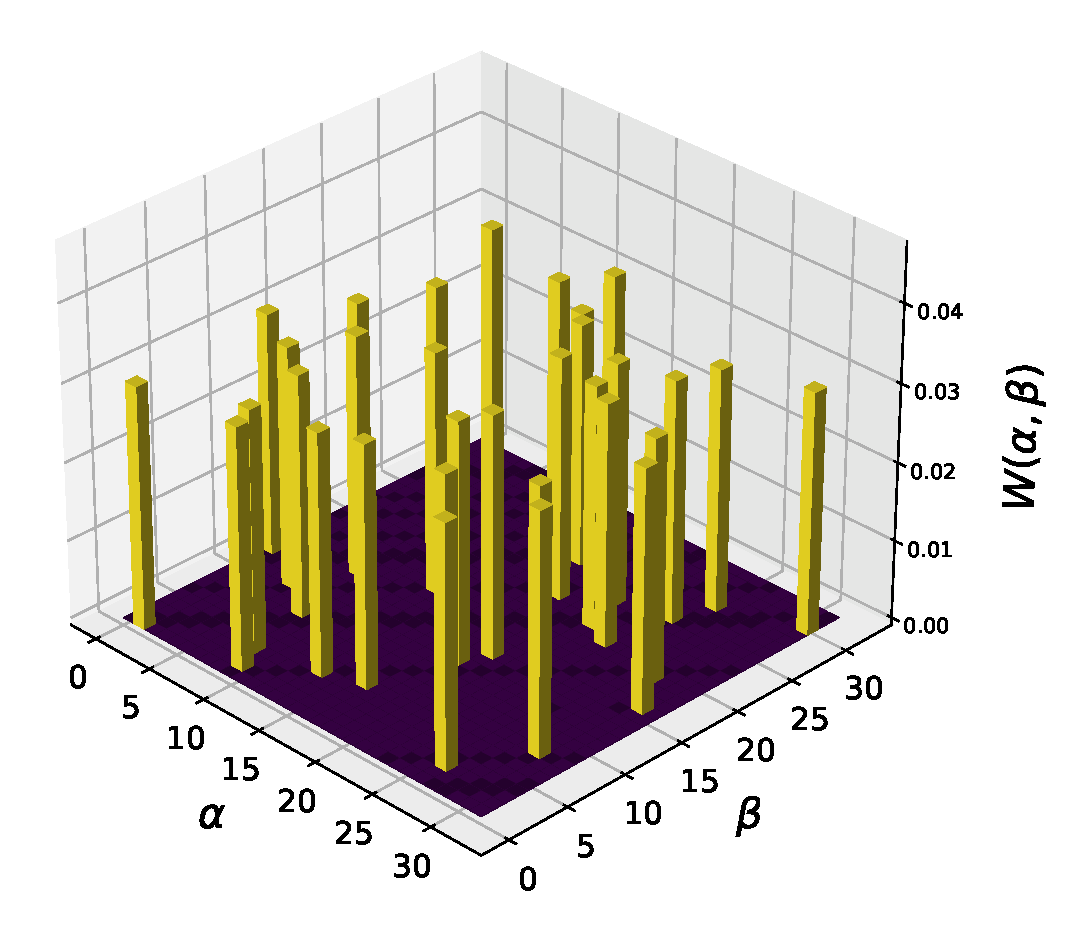
\includegraphics[scale=0.35]{
        paper/pres_graphs/32_woo.eps
      }
      \caption{
        Función de Wigner estándar para $\ket{\psi_1}$.
      }
      \label{fig:wigner-standard-2-5-s1}
    \end{figure}
  \end{frame}

  \begin{frame}
    \frametitle{Funciones de Wigner para cinco qubits}

    \begin{figure}[h]
      \centering
      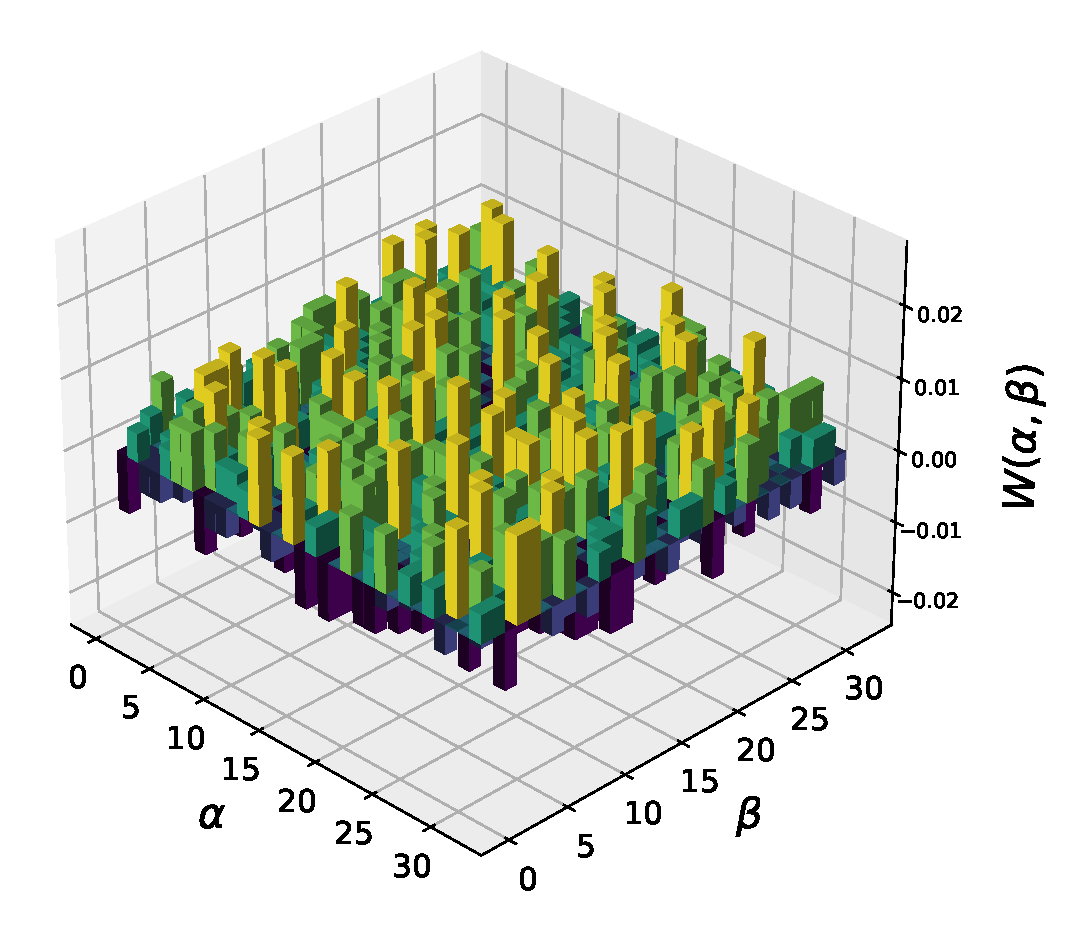
\includegraphics[scale=0.35]{
        paper/pres_graphs/32_kan.eps
      }
      \caption{
        Función de Wigner no estándar para $\ket{\psi_1}$.
      }
      \label{fig:wigner-kantor-2-5-s1}
    \end{figure}
  \end{frame}

  \begin{frame}
    \frametitle{Funciones de Wigner para cinco qubits}

    \begin{figure}[h]
      \centering
      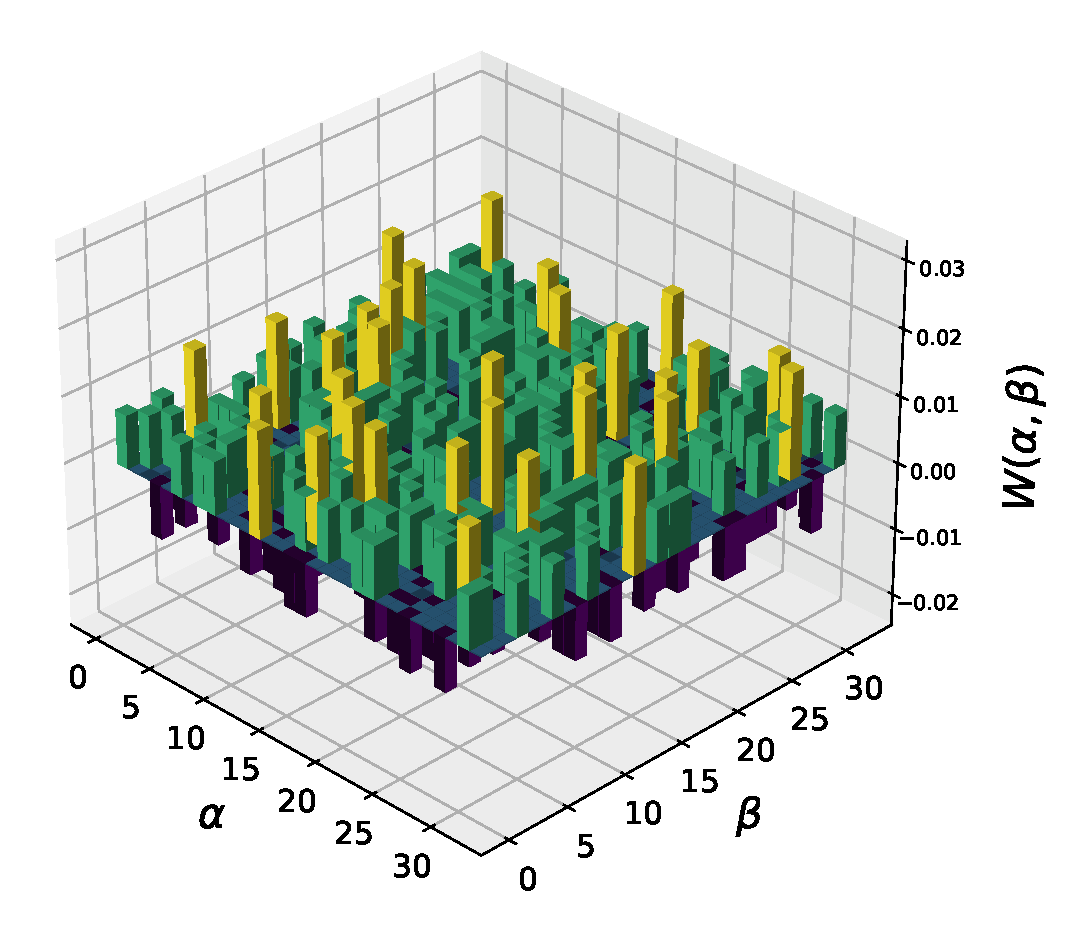
\includegraphics[scale=0.35]{
        paper/pres_graphs/32_woo_2.eps
      }
      \caption{
        Función de Wigner no estándar para $\ket{\psi_2}$.
      }
      \label{fig:wigner-kantor-2-5-s2}
    \end{figure}
  \end{frame}

  \begin{frame}
    \frametitle{Funciones de Wigner para cinco qubits}

    \begin{figure}[h]
      \centering
      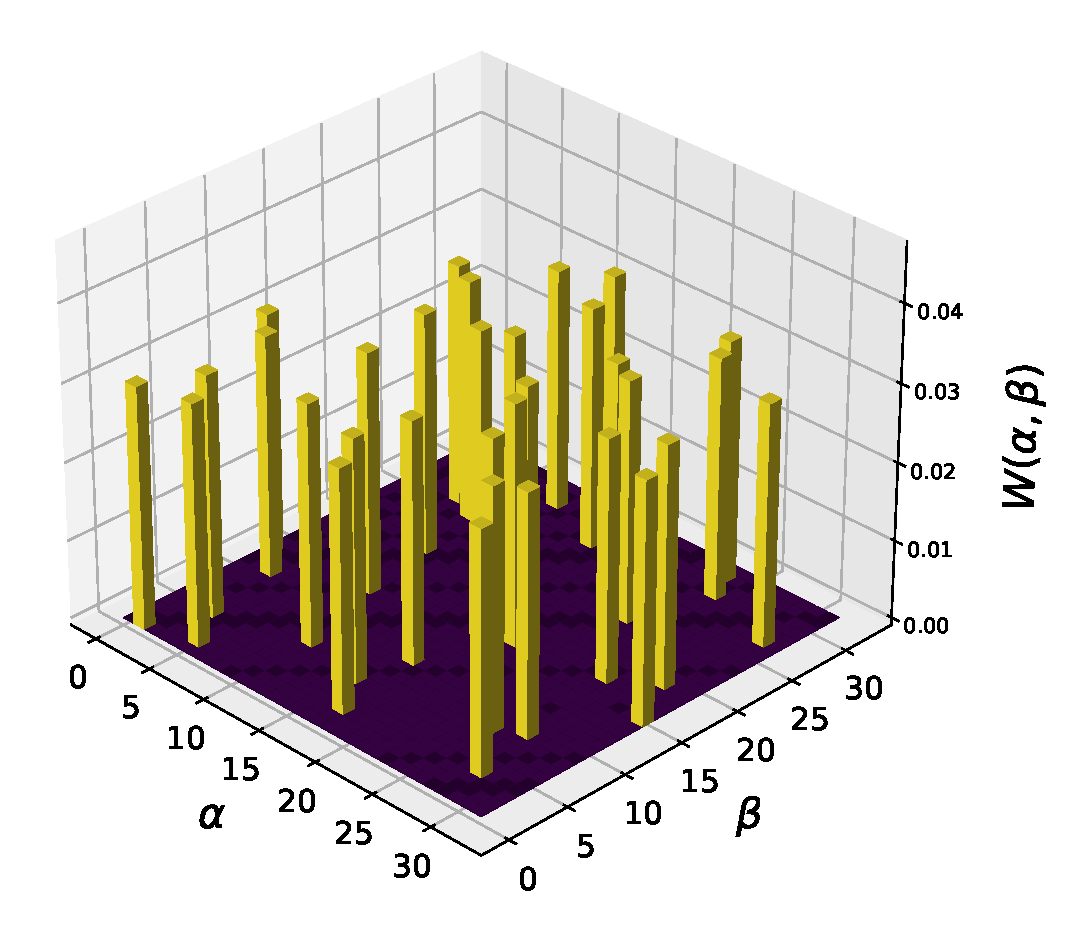
\includegraphics[scale=0.35]{
        paper/pres_graphs/32_kan_2.eps
      }
      \caption{
        Función de Wigner estándar para $\ket{\psi_2}$.
      }
      \label{fig:wigner-standard-2-5-s2}
    \end{figure}
  \end{frame}

  \begin{frame}
    \frametitle{Funciones de Wigner para cinco qubits}

    \begin{figure}[h]
      \centering
      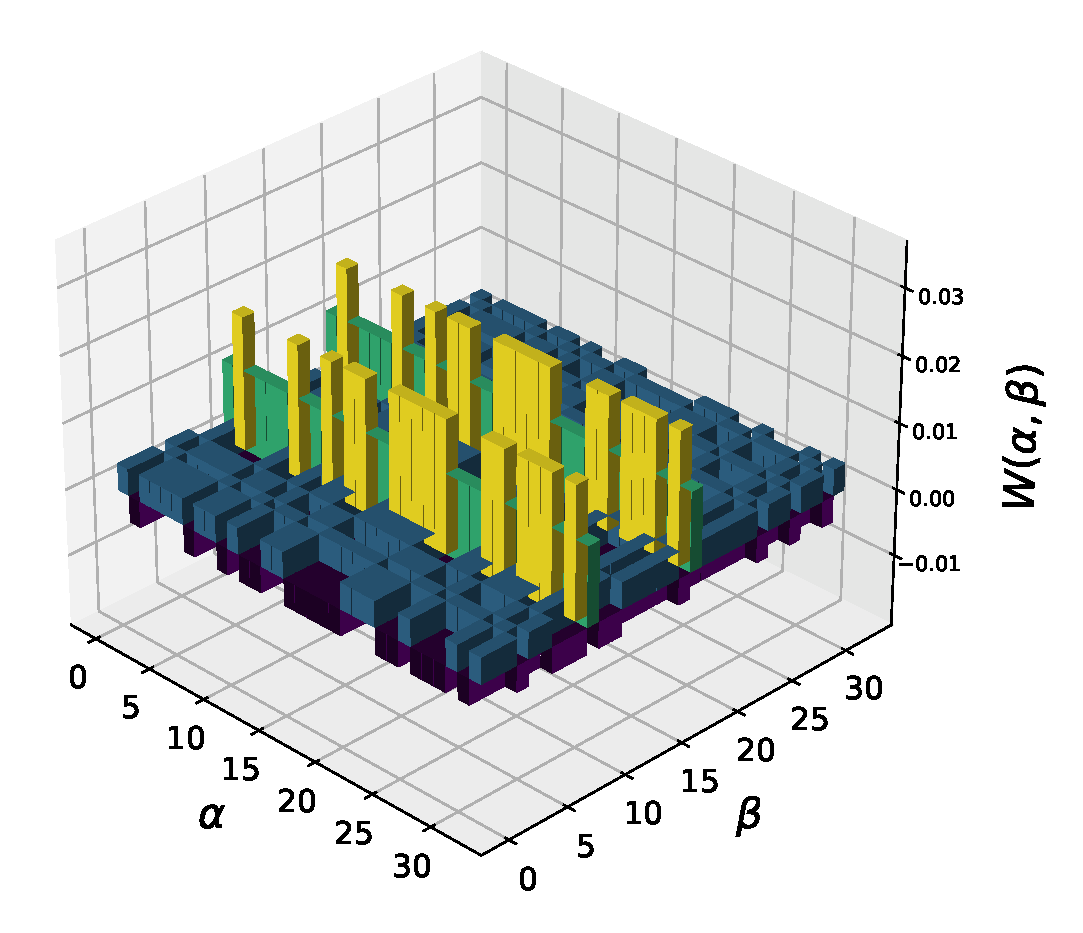
\includegraphics[scale=0.35]{
        paper/pres_graphs/32_woo_3.eps
      }
      \caption{
        Función de Wigner estándar para $\ket{\psi_3}$.
      }
      \label{fig:wigner-standard-2-5-s3}
    \end{figure}
  \end{frame}

  \begin{frame}
    \frametitle{Funciones de Wigner para cinco qubits}

    \begin{figure}[h]
      \centering
      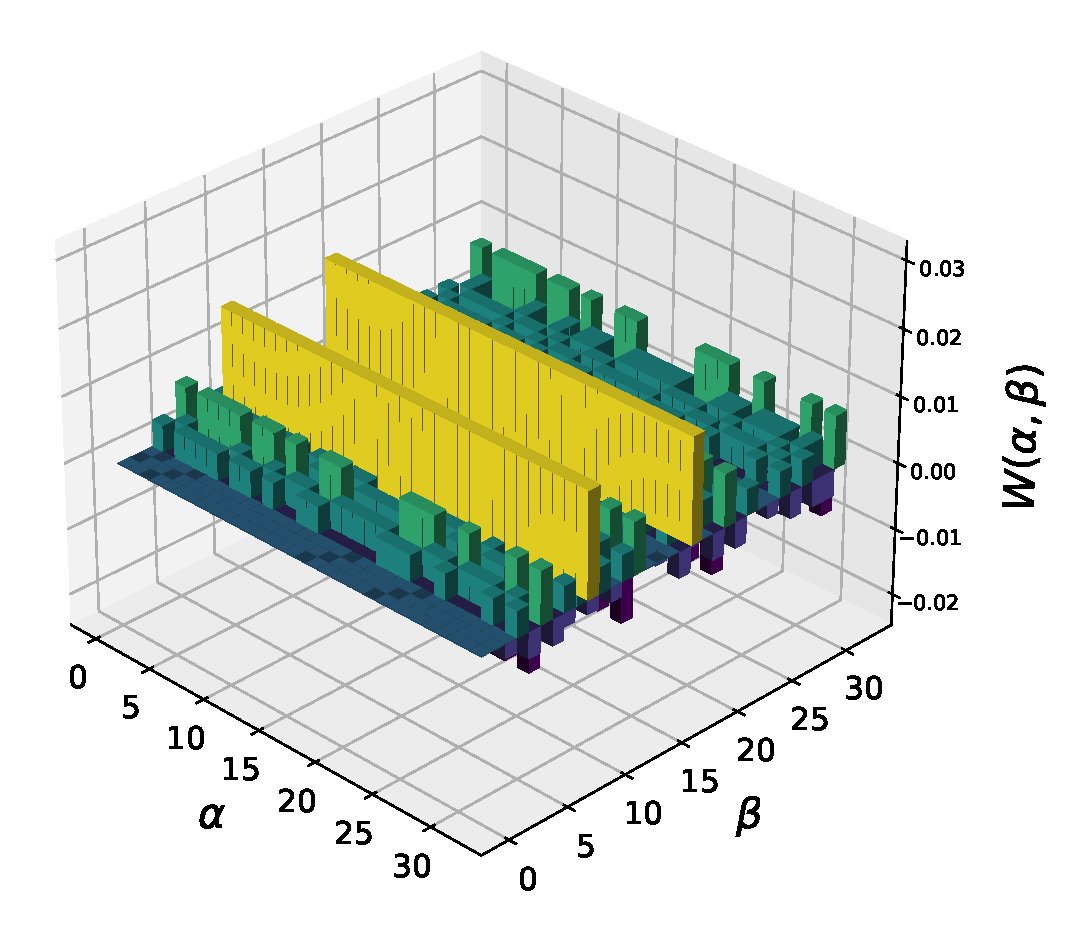
\includegraphics[scale=0.35]{
        paper/pres_graphs/32_kan_3.eps
      }
      \caption{
        Función de Wigner no estándar para $\ket{\psi_3}$.
      }
      \label{fig:wigner-kantor-2-5-s3}
    \end{figure}
  \end{frame}

  %%%%%%%%%%%%%%%%%%%%%%%%%%%%%%%%%%%%%%%%%%%%%%%%%%%

  \begin{frame}
    \frametitle{Funciones de Wigner para tres qutrits}

    Construímos la función de Wigner estándar y no estándar
    para un sistema de tres qutrits, $\H = \C^{27} \cong
    \left( \C^{3} \right)^{\otimes 3}$. Como ejemplo
    consideramos un elemento $\ket{\psi}$ de las MUBs del
    campo torcido de Albert.
  \end{frame}

  \begin{frame}
    \frametitle{Funciones de Wigner para tres qutrits}

    \begin{figure}[h]
      \centering
      \subfloat[Núcleo estándar]{
        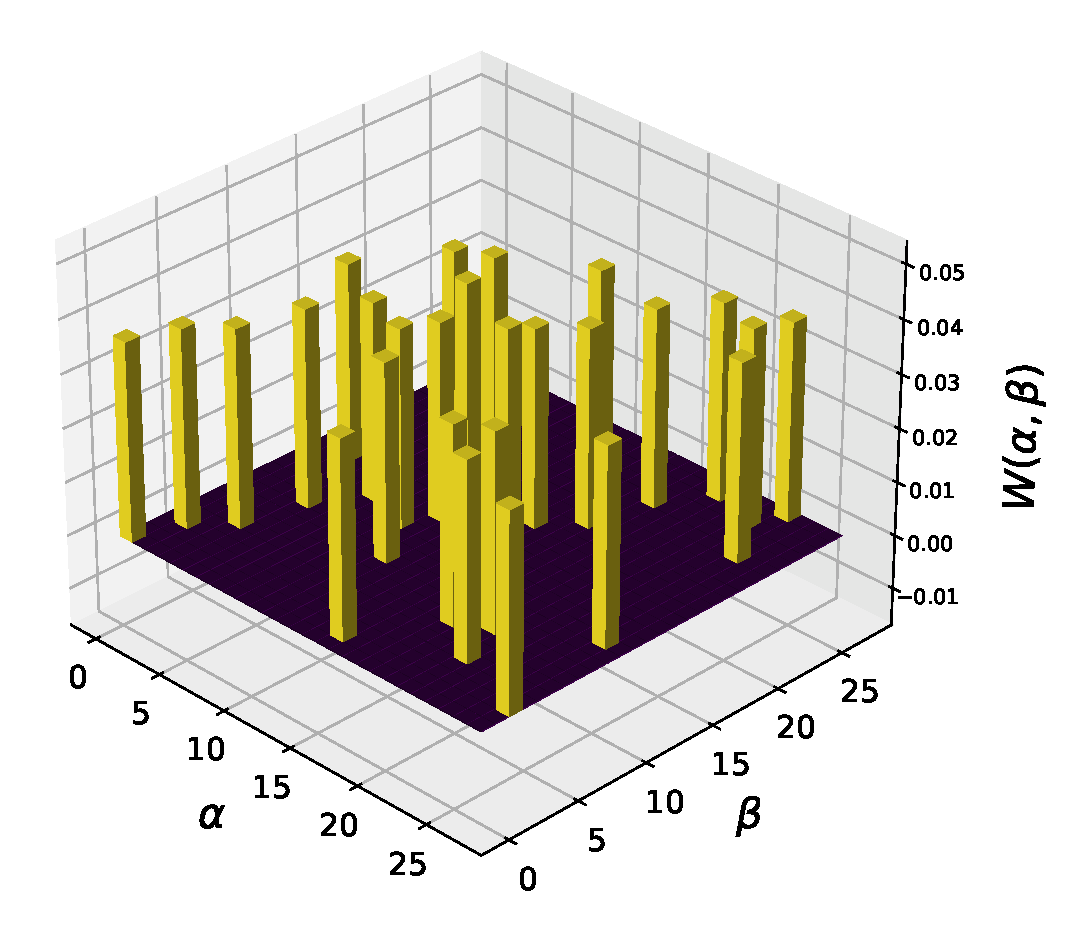
\includegraphics[scale=0.3]{
          paper/pres_graphs/27_both.eps
        }
      }
      \subfloat[Núcleo no estándar]{
        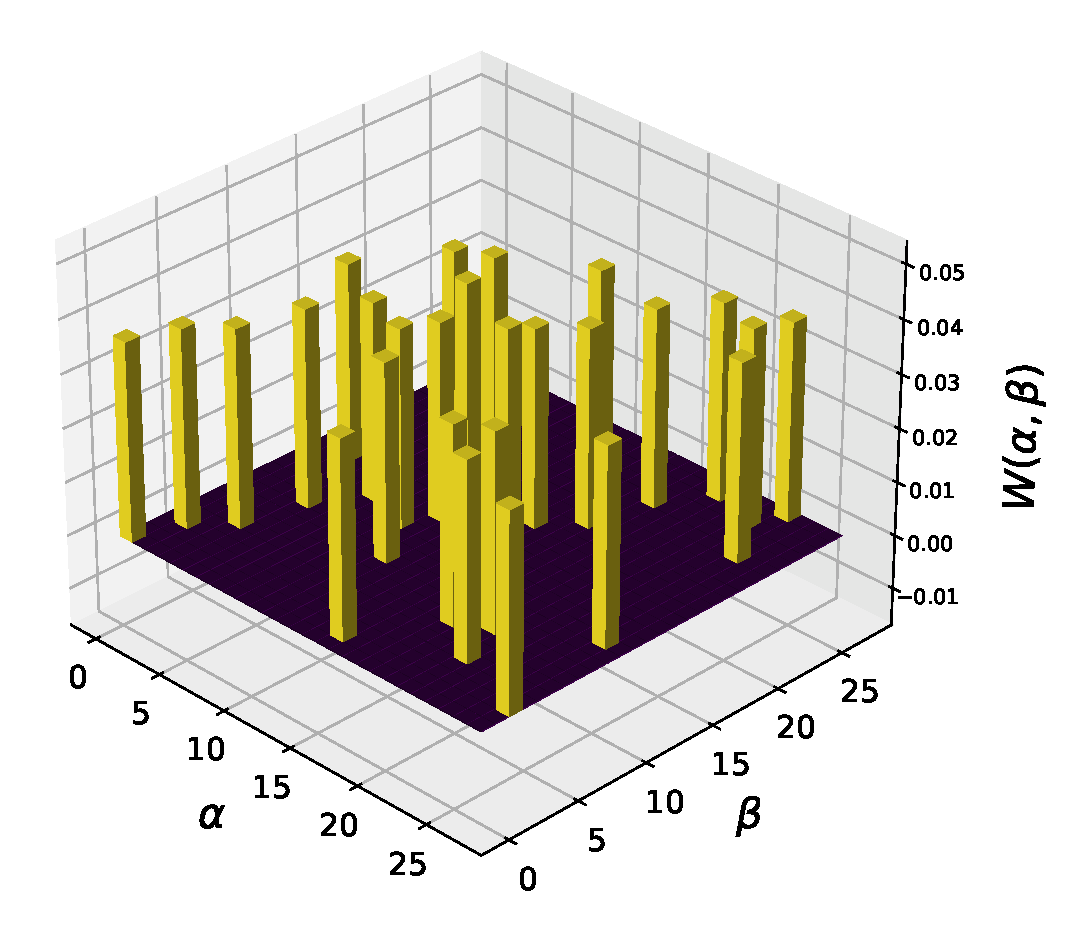
\includegraphics[scale=0.3]{
          paper/pres_graphs/27_both.eps
        }
      }
      \caption{
        Función de Wigner para el estado $\ket{\psi}$.
      }
      \label{fig:wigner-kantor-3-3-s1}
    \end{figure}
  \end{frame}

  \section{Discusión}

  \begin{frame}
    \frametitle{Equivalencia de los núcleos en el caso de
      los qutrits}

    Utilizando unos resultados sobre sumas Gaussianas de
    los caracteres aditivos $\chi(\alpha)$ del campo,
    demostramos que el núcelo formado por los rayos es
    \textit{idéntico} al núcleo formado por la cobertura de
    Albert
    \begin{equation}
      \hat A(\alpha,\beta) = \hat A'(\alpha,\beta).
    \end{equation}

    \vspace{15pt}

    \pause

    Éste resultado implica que la inequivalencia unitaria
    de los MUBs formados por coberturas no equivalentes, no
    es suficiente para obtener una función de Wigner
    distinta.

    \vspace{5pt}

    Más aún, debe ser posible extender éste resultado a
    \textit{cualquier} cobertura simpléctica. 
  \end{frame}

  \begin{frame}
    \frametitle{Negatividad de la función de Wigner}

    La negatividad de la función de Wigner ha sido
    utilizada para identificar que tán ``cuántico'' es
    nuestro sistema.

    \vspace{5pt}

    %Debido a que la función de Wigner es
    %covariante bajo transformaciones simplécticas en el
    %caso de los qudits, obtenemos un resultado análogo al
    %caso continuo para estados gaussianos.

    \begin{theorem}[Teorema de Hudson para sistemas finitos]
      Para un sistema de $n$-qudits con dimensión local
      impar, los estados estabilizadores corresponden a
      funciones de Wigner no-negativas.
    \end{theorem}

    \vspace{5pt}

    \pause

    Un resultado análogo para el caso de $n$-qubits
    \textbf{no es posible}, ya que la no-negatividad de
    $W_{\hat\rho}$ de un estabilizador depende directamente
    de la partición del DPS utilizada para construir el
    núcleo de Wigner!
    
  \end{frame}

  \begin{frame}
    \frametitle{Discusión}

    \begin{itemize}
      \item Equivalencia de las funciones de Wigner
        discretas.
      \pause
      \item Generalización a dimensiones arbitrarias.
        \begin{itemize}
          \item Descomposición ortogonal de
            $\mathfrak{sl}_d(\C)$.
          \item Planos afínes
          \item MOLS.
        \end{itemize}
      \pause
      \item Dinámica en el espacio de fase discreto.
      \pause
      \item Esquemas de factorización tensorial.
    \end{itemize}
  \end{frame}

  \begin{frame}
    \frametitle{Fin}

    Gracias por su atención!
  \end{frame}

  \section*{}
  \appendix

  %\begin{frame}[allowframebreaks]
  %  \frametitle{Referencias}

  %  \nocite{*}
  %  \printbibliography
  %\end{frame}

  % END

  \begin{frame}
    \frametitle{Postulados de la mecánica cuántica}

    \begin{enumerate}
      \item A cada sistema cuántico le corresponde un
        espacio de Hilbert $\H$. Los estados $\ket\psi$ del
        sistema son vectores unitarios de $\H$.
      \item A cada observable físico $A$ le corresponde un
        observable cuántico representado por un operador
        auto-adjunto $\hat A$.
      \item El valor esperado del observable $A$ del sistema
        en estado $\psi$ está dado por:
        \begin{equation}
          \braket{\hat A}_\psi := \braket{\psi|\hat A|\psi}.
        \end{equation}
      \item La probabilidad de observar un valor $\lambda$ 
        al medir el observable físico $A$, en el estado
        $\psi$ está dado por la regla de Born:
        \begin{equation}
          \Pr(\lambda)
          = |\braket{\psi|\phi_\lambda}|^2,
        \end{equation}
        donde $\phi_\lambda$ es el eigenestado de $\hat A$ 
        con eigenvalor $\lambda$.
    \end{enumerate}
  \end{frame}

  \begin{frame}
    \frametitle{Cuasi-distribuciones}

    En la mecánica clásica podemos calcular el valor
    esperado de un observable $A$ utilizando una densidad
    probabilística correspondiente a un conjunto de
    partículas:
    \begin{equation}
      \mathbb E(A)
      = \iint A(x,p) F(x,p) \, dx \, dp.
    \end{equation}

    \vspace{10pt}

    Utilizando las cuasi-distribuciones podemos cálcular el
    valor esperado de un observable cuántico $\hat A$ en un
    estado $\hat \rho$ de manera similar:
    \begin{equation}
      \Tr\left( \hat A \hat \rho \right)
      = \iint A(x,p) W(x,p) \, dx \, dp.
    \end{equation}
  \end{frame}

  \begin{frame}
    \frametitle{Determinación de un estado cuántico}
    
    El problema de la determinación de estados cuánticos, (ó
    de tomografía cuántica), es el problema de determinar la
    matriz de densidad correspondiente a un ensamble de
    sistemas identicamente preparados.

    \vspace{15pt}

    La matriz de densidad está determinada por $d^2 - 1$
    parámetros reales. Una medición en una base nos genera
    $d-1$ números reales independientes. Por lo tanto
    requerimos de al menos $d+1$ distintas mediciones para
    recuperar el estado cuántico.
  \end{frame}

  \begin{frame}
    \frametitle{Presemicampos y semicampos}

    \begin{definition}
      Un \textit{presemicampo} es un anillo sin divisores
      del cero, excepto que la asociatividad no es
      necesaria. Un \textit{semicampo} es un presemicampo
      con una identidad multiplicativa.
    \end{definition}

    \vspace{5pt}

    Siempre podemos obtener un presemicampo finito $(\F,
    +,\circ)$ a partir de un campo finito $(\F,+,\cdot)$
    introduciendo una nueva operación binaria $\circ$.
  \end{frame}

  \begin{frame}
    \frametitle{Anillo de Galois y el conjunto Teichmüller}

    Sea $R = \GR(4^{n})$ el anillo de Galois de
    caraterística $4$. Existe un elemento $\xi$ que es
    una $2^{n}-1$-ésima raíz primitiva de la unidad.

    \vspace{5pt}

    \begin{definition}
      El conjunto \textit{Teichmüller} $\mathcal T \subset
      R$ está dado por
      \begin{equation}
        \mathcal T
        = \{0,1,\xi,\xi^2,\ldots,\xi^{2^{n}-2}\},
      \end{equation}
      donde $\mathcal T \setminus \{0\}$ es un subgrupo
      multiplicativo isomorfo a $\F$.
    \end{definition}

    \vspace{5pt}

    Todo elemento $x \in R$ tiene una representación
    $2$-ádica, $x = a + 2b$ donde $a,b \in \mathcal T$.
  \end{frame}

  \begin{frame}
    \frametitle{Construcción de MUBs: característica impar}

    \begin{theorem}
      Sea $\F$  y $(\F,+,\circ)$ un presemicampo simpléctico
      de característica impar, entonces los conjuntos
      \begin{equation}
        B_\infty
        = \{\ket{e_w} : w \in \F\},
        \quad
        B_m
        = \{\ket{b_{m,v}} : v \in \F\},
      \end{equation}
      donde
      \begin{equation}
        \ket{b_{m,v}}
        = \frac{1}{\sqrt{d}} 
        \sum_{w \in \F}^{} \omega^{\tr\left(\frac{1}{2} w
        (w\circ m) + vw\right)} \ket{e_w},
      \end{equation}
      para todo $m \in F$ forman un conjunto completo de
      MUBs.
    \end{theorem}
  \end{frame}

  \begin{frame}
    \frametitle{Construcción de MUBs: característica par}

    \begin{theorem}
      Sea $\F$  y $(\F,+,\circ)$ un presemicampo simpléctico
      de característica par, entonces los conjuntos
      \begin{equation}
        B_\infty
        = \{\ket{e_w} : w \in \F\},
        \quad
        B_m
        = \{\ket{b_{m,v}} : v \in \F\},
      \end{equation}
      donde
      \begin{equation}
        \ket{b_{m,v}}
        = \frac{1}{\sqrt{d}} 
        \sum_{w \in \F}^{} \omega^{\tr\left( \hat w (\hat
        w\circ \hat m) + 2\hat v \hat w\right)} \ket{e_w},
      \end{equation}
      para todo $m \in F$ forman un conjunto completo de
      MUBs, donde $\hat x$ es el lift al Teichmüller
      $\mathcal T$ del elemento $x \in \F$.
    \end{theorem}

  \end{frame}

  \begin{frame}[fragile]
    \frametitle{Detalles de la implementación}

    Para poder hacer los cálculos necesarios para la
    construcción de las MUBs y de las funciones de Wigner,
    fue necesario utilizar un software con la capacidad de
    computar con campos finitos.

    \vspace{5pt}

    Para ésto utilizamos el software libre
    \texttt{SageMath} y su sub-módulo de extensiones de
    Galois y cocientes de anillos.

    \vspace{5pt}

    \begin{example}
      Construcción del anillo de Galois $\GR(4,5)$.

      \begin{verbatim}
        R = PolynomialRing(Integers(4), 't')
        t = R.gen()
        GR = R.quotient(t**5 + 3*t**2 + 2*t + 3, 'w')
        w = GR.gen()
      \end{verbatim}
    \end{example}
  \end{frame}
\end{document}
